%%%%%%%%%%%%%%%%%%%%%%%%%%%%%%%%%%%%%%%%%%%%%%%%%%%%%%%%%%%%%%%%%%%%%%%%%%%%%%%%
%                                                                              %
%   PAW Guide/ Reference Manual -- LaTeX Source                                %
%                                                                              %
%   Main driver file. Includes other files of manual,                          %
%   generates table of contents and includes index file.                       %
%                                                                              %
%   To run, you need the CERN style  cernman.sty                               %
%                                                                              %
%   Editor: Michel Goossens / IT-ASD                                           %
%   Last Mod.: 30 July 1998  Olivier Couet                                     %
%                                                                              %
%%%%%%%%%%%%%%%%%%%%%%%%%%%%%%%%%%%%%%%%%%%%%%%%%%%%%%%%%%%%%%%%%%%%%%%%%%%%%%%%
\documentclass[10pt]{cernman}
\usepackage{fancyvrb}
\usepackage{pawdefs}
\usepackage{longtable}
\usepackage[dvips]{rotating}
\let\finalnewpage\clearpage
\let\finalclearpage\clearpage
\graphicspath{{../epsfiles/}}
\setlongtables
\renewcommand{\textfraction}{.05}
\renewcommand{\topfraction}{.95}
\renewcommand{\floatpagefraction}{.80}
\setcounter{totalnumber}{4}
\setcounter{topnumber}{3}
\makeindex
\DefineVerbatimEnvironment{alltt}{Verbatim}%
                          {fontsize=\small,commandchars=\\\{\},%
                           xleftmargin=0pt}
\DefineVerbatimEnvironment{falltt}{Verbatim}%
                          {fontsize=\footnotesize,commandchars=\\\{\},%
                           xleftmargin=0pt}
\DefineVerbatimEnvironment{salltt}{Verbatim}%
                          {fontsize=\scriptsize,commandchars=\\\{\},%
                           xleftmargin=0pt}
\DefineVerbatimEnvironment{talltt}{Verbatim}%
                          {fontsize=\tiny,commandchars=\\\{\},%
                           xleftmargin=0pt}
\DefineVerbatimEnvironment{verbatim}{Verbatim}%
                          {fontsize=\small,xleftmargin=0pt}
\begin{document}
%  ==================== Front material ============================

%%%%%%%%%%%%%%%%%%%%%%%%%%%%%%%%%%%%%%%%%%%%%%%%%%%%%%%%%%%%%%%%%%%
%                                                                 %
%   PAW   - Reference Manual -- LaTeX Source                      %
%                                                                 %
%   Front Material: Title page,                                   %
%                   Copyright Notice                              %
%                   Preliminary Remarks                           %
%                   Table of Contents                             %
%   EPS file      : cernlogo.eps                                  %
%                                                                 %
%   Editor: Michel Goossens / CN-AS                               %
%   Last Mod.: 16 August 1993 09:00 mg                            %
%                                                                 %
%%%%%%%%%%%%%%%%%%%%%%%%%%%%%%%%%%%%%%%%%%%%%%%%%%%%%%%%%%%%%%%%%%%
 
%%%%%%%%%%%%%%%%%%%%%%%%%%%%%%%%%%%%%%%%%%%%%%%%%%%%%%%%%%%%%%%%%%%%
%    Title page                                                    %
%%%%%%%%%%%%%%%%%%%%%%%%%%%%%%%%%%%%%%%%%%%%%%%%%%%%%%%%%%%%%%%%%%%%
\def\Ptitle#1{\special{ps: /Printstring (#1) def}
\epsfbox{cnastit.eps}}
 
\begin{titlepage}
\vspace*{-23mm}
\mbox{\epsfysize30mm\epsfbox{cern15.eps}}
\hfill
\raise8mm\hbox{\Large\bf CERN Program Library Long Writeup Q121}
\hfill\mbox{}
\begin{center}
\mbox{}\\[10mm]
\mbox{\Ptitle{PAW}}\\[2cm]
{\Huge Physics Analysis Workstation}\\[2cm]
{\Huge User's guide}\\[5cm]
%%%{\Large Application Software Group}\\[3mm]
{\Large Information Technology Division}\\[2cm]
\end{center}
\vfill
\begin{center}\Large CERN, Geneva, Switzerland\end{center}
\end{titlepage}
 
%%%%%%%%%%%%%%%%%%%%%%%%%%%%%%%%%%%%%%%%%%%%%%%%%%%%%%%%%%%%%%%%%%%%
%    Copyright  page                                               %
%%%%%%%%%%%%%%%%%%%%%%%%%%%%%%%%%%%%%%%%%%%%%%%%%%%%%%%%%%%%%%%%%%%%

\thispagestyle{empty}
\framebox[\textwidth][t]{\hfill\begin{minipage}{0.96\textwidth}%
\vspace*{3mm}\begin{center}Copyright Notice\end{center}
\parskip\baselineskip
{\bf PAW -- Physics Analysis Workstation}
 
CERN Program Library entry {\bf Q121}
 
\copyright{} Copyright CERN, Geneva 1992--1999
 
Copyright and any other appropriate legal protection of these
computer programs and associated documentation reserved in all
countries of the world.
 
These programs or documentation may not be reproduced by any
method without prior written consent of the Director-General
of CERN or his delegate.
 
Permission for the usage of any programs described herein is
granted apriori to those scientific institutes associated with
the CERN experimental program or with whom CERN has concluded
a scientific collaboration agreement.
 
Requests for information should be addressed to:
\vspace*{-.5\baselineskip}
\begin{center}
\tt\begin{tabular}{l}
CERN Program Library Office              \\
CERN-IT Division                         \\
CH-1211 Geneva 23                        \\
Switzerland                              \\
Tel.      +41 22 767 4951                \\
Fax.      +41 22 767 8630                \\
Internet: cernlib@cern.ch
\end{tabular}
\end{center}
\vspace*{2mm}
\end{minipage}\hfill}%end of minipage in framebox
\vspace{6mm}
 
{\bf Trademark notice:} All trademarks appearing in this guide are acknowledged as such.
\vfill

\begin{tabular}{l@{\quad}l@{\quad}>{\tt}l}
\emph{Contact Person}:       & Olivier Couet   & (Olivier.Couet\atsign   cern.ch)\\[1mm]
\emph{Document Consultant}: & Michel Goossens & (Michel.Goossens\atsign cern.ch)\\[1cm]
{\em Edition -- January 1999}
\end{tabular}

\newpage
 
%%%%%%%%%%%%%%%%%%%%%%%%%%%%%%%%%%%%%%%%%%%%%%%%%%%%%%%%%%%%%%%%%%%%
%    Introductory material                                         %
%%%%%%%%%%%%%%%%%%%%%%%%%%%%%%%%%%%%%%%%%%%%%%%%%%%%%%%%%%%%%%%%%%%%
\pagenumbering{roman}
\setcounter{page}{1}
 
\chapter*{About this guide}
 
\section*{Preliminary remarks}
 
In this manual
examples are in \Lit{monotype face} and strings to be input by the user
are \Ucom{underlined}.
In the index the page where a command is defined is in {\bf bold},
page numbers where a routine is referenced are in normal type.
 

\section*{Related Manuals}
 
This document can be complemented by the following manuals:
 
\begin{UL}
\item COMIS, Compilation and Interpretation System~\cite{bib-COMIS}
\item HBOOK User Guide --- Version 4~\cite{bib-HBOOK}
\item HIGZ-HPLOT --- High level Interface to Graphics and ZEBRA and
                 HPLOT User Guide~\cite{bib-HIGZHPLOT}
\item KUIP --- Kit for a User Interface Package~\cite{bib-KUIP}
\item MINUIT --- Function Minimization and Error Analysis~\cite{bib-MINUIT}
\item ZEBRA --- Data Structure Management System~\cite{bib-ZEBRA}
\end{UL}
 
This document present the basic concepts of PAW. For more detailed and
up to date informations on the system it is strongly recommended to
look at the following URL:

\begin{center}\ttfamily
http://wwwcn.cern.ch/pl/paw/
\end{center}

\section*{Acknowledgements}
 
The authors of PAW would like to thank all their colleagues who, by their
continuous interest and encouragement, have given them the necessary input 
to provide a modern and easy to use data analysis and presentation system.

%%%%%%%%%%%%%%%%%%%%%%%%%%%%%%%%%%%%%%%%%%%%%%%%%%%%%%%%%%%%%%%%%%%%
%    Tables of contents ...                                        %
%%%%%%%%%%%%%%%%%%%%%%%%%%%%%%%%%%%%%%%%%%%%%%%%%%%%%%%%%%%%%%%%%%%%
\newpage
\setcounter{tocdepth}{2}
\tableofcontents
\endinput
\cleardoublepage
%  ==================== Body of text ==============================
\pagenumbering{arabic}
\setcounter{page}{1}
%%%% **************** Start of part 1 **************************-- >
%\part{PAW - Commands and Concepts}
%\part{PAW -- Step by step}
%\mbox{}\thispagestyle{empty}\newpage
%%%%%%%%%%%%%%%%%%%%%%%%%%%%%%%%%%%%%%%%%%%%%%%%%%%%%%%%%%%%%%%%%%%%%%%%%%%%%%%%
%                                                                              %
%   PAW   - Reference Manual -- LaTeX Source                                   %
%                                                                              %
%   Chapter 1: A few words on PAW                                              %
%                                                                              %
%   EPS file      : pawtut01.eps                                               %
%                   pawtut00.eps                                               %
%                                                                              %
%   Editor: Michel Goossens / IT-ASD                                           %
%   Last Mod.: 30 July 1998 Olivier Couet                                      %
%                                                                              %
%%%%%%%%%%%%%%%%%%%%%%%%%%%%%%%%%%%%%%%%%%%%%%%%%%%%%%%%%%%%%%%%%%%%%%%%%%%%%%%%

\chapter{A few words on PAW}
\label{sec:intro}
 
\section{A short history}

At the beginning of 1986 the {\bf P}hysics {\bf A}nalysis {\bf W}orkstation 
project {\bf PAW} was launched at CERN. The first public release of the system 
was made at the beginning of 1988. At present the system runs on most of the 
computer systems used in the High Energy Physics (HEP) community (Mainframes, 
Workstations, PC's). In addition to its powerful data analysis, particular 
emphasis has been put on the quality of the user interface and of the graphical
presentation.
 
\section{What is PAW?}
 
PAW is an interactive utility for visualizing experimental data on a computer 
graphics display. \index{batch} \index{interactive} It may be run in batch mode
if desired for very large and time consuming data analyses; typically, however,
the user will decide on an analysis procedure interactively before running a 
batch job.
 
PAW combines a handful of CERN High Energy Physics Library systems that may also
used individually in software that processes and displays data. The purpose of 
PAW is to provide many common analysis and display procedures that would be 
duplicated needlessly by individual programmers, to supply a flexible way to 
invoke these common procedures, and yet also to allow user customization where
necessary.
 
\section{What Can You Do with PAW?}
 
PAW can do a wide variety of tasks relevant to analyzing and understanding 
physical data, which are typically statistical distributions of measured events.
Below we list what are probably the most frequent and best-adapted applications
of PAW; the list is not intended to be exhaustive, for it is obviously possible
to use PAW's flexibility to do a huge number of things, some more difficult to 
achieve than others within the given structure.
 
\subsubsection*{Typical PAW Applications:}
 
\begin{itemize}
\item {\bf Plot a Vector of Data Fields for a List of Events.}
      A set of raw data is typically processed by the user's own software to
      give a set of physical quantities, such as momenta, energies, particle
      identities, and so on, for each event.  When this digested data is saved 
      on a file as an Ntuple, it may be read and manipulated directly from PAW. 
      Options for plotting Ntuples include the following:
 
\begin{itemize}
\item {\it One Variable.\/}  If a plot of a one variable from the data set is 
      requested, a histogram showing the statistical distribution of the values
      from all the events is automatically created. Individual events are not
      plotted, but appear only as a contribution to the corresponding 
      histogram bin.
\item {\it Two or Three Variables.\/}  If a plot of two or three variables from
      the data set is requested, no histogram is created, but a 2D or 3D scatter
      plot showing a point or marker for each distinct event is produced.
\item {\it Four Variables.\/}  If a plot
      of four variables is requested, a 3D scatter plot of the first three
      variables is produced, and a color map is assigned to the fourth variable;
      the displayed color of the individual data points in the 3D scatter plot 
      indicates the approximate value of the fourth variable.
\item {\it More than Four Variables.\/}  More than four variables can be plotted
      but it is up to the user to customize the system in order to assign the 
      additional variables to graphics attributes like the size or the shape 
      (type) of the markers.
\item {\it Vector Functions of Variables.\/}  PAW allows the user to define 
      arbitrary vector functions of the original variables in an Ntuple, and to
      plot those instead of the bare variables. Thus one can easily plot 
      something
      like \(\sqrt{(P_{x}^{2} + P_{y}^{2})}\) if \(P_{x}\) and \(P_{y}\) are
      original variables in the data without having to add a new data field to 
      the Ntuple at the time of its creation.
\item {\it Selection Functions (Cuts).\/}  PAW does not require you to use every
      event in your data set. Several methods are provided to define Boolean 
      functions of the variables themselves that pick out subsets of the events 
      to be included in a plot.
\item {\it Plot presentation options.\/} The PAW user can set a variety of 
      options to customize the format and appearance of the plots.
\end{itemize}
 
\item {\bf Histogram of a Vector of Variables for a List of Events.}
      Often one is more interested in the statistical distribution of a vector 
      of variables (or vector functions of the variables) than in the variables
      themselves.  PAW provides utilities for defining the desired limits and 
      bin characteristics of a histogram and accumulating the bin counts by 
      scanning through a list of events. The following are some of the features
      available for the creation of histograms:
 
\begin{itemize}
\item {\it One Dimensional Histograms.\/} Any single variable can be analyzed 
      using a one-dimensional histogram that shows how many events lie in each 
      bin. This is basically equivalent to the single-variable data plotting 
      application except that it is easier to specify personalized features of 
      the display format. A variety of features allow the user to slice and 
      project a 2D scatter plot and make a 1D histogram from the resulting 
      projection.
\item {\it  Two-Dimensional Histograms.\/} The distribution of any pair of 
      variables for a set of events can be accumulated into a 2D histogram and 
      plotted in a various of ways to show the resulting surface.
\item {\it Vector Functions of Variables.\/} User-defined functions of variables      in each event can be used to define the histogram, just as for an Ntuple 
      plot.
\item {\it Selection Functions (Cuts).\/} Events may also be included or 
      excluded by invoking Boolean selection functions that are arbitrary 
      functions of the variables of a given event.
\item {\it Event Weights.\/} PAW allows the user to include a multiplicative 
      statistical bias for each event which is a scalar function of the 
      available variables. This permits the user to correct for known 
      statistical biases in the data when making histograms of event 
      distributions.
\item {\it Histogram Presentation Options.\/} Virtually every aspect of the 
      appearance of a histogram can be controlled by the user.  Axis labels, 
      tick marks, titles, colors, fonts, and so on, are specified by a large 
      family of options.
\end{itemize}
 
\item {\bf Fit a Function to a Histogram.}  Once a histogram is defined, the 
      user may fit the resulting shape with one of a family of standard 
      functions, or with a custom-designed function.  The parameters of the fit
      are returned in user-accessible form.  Fitted functions of one variable
      may be attached to a 1D histogram and plotted with it.  The capability of
      associating fits to higher dimensional histograms and overlaying their
      representations on the histogram is in the process of being added to PAW.
 
      The fitting process in PAW is normally carried out by the MINUIT library.
      To user this package effectively, users must typically supply data with
      reasonable numerical ranges and give reasonable initial conditions for the
      fit before passing the task to the automated procedure.
 
\item {\bf Annotate and Print Graphics.} A typical objective of a PAW user is 
      to examine, manipulate, and display the properties of a body of
      experimental data, and then to prepare a graph of the results for use in
      a report, presentation, or publication.  PAW includes for convenience a
      family of graphics primitives and procedures that may be used to annotate
      and customize graphics for such purposes.  In addition, any graphics
      display presented on the screen can be converted to a PostScript file for
      black-and-white or color printing, or for direct inclusion in a
      manuscript.
 
\end{itemize}
 
\section{A User's View of PAW}
 
In order to take advantage of PAW, the user must first have an understanding of
its basic structure.  Below we explain the fundamental ways in which PAW and the
user interact.
 
\paragraph{Initialization.}  PAW may be invoked in a variety of ways, depending
on the user's specific computer system; these are described in the following 
chapter.  As PAW starts, it prompts the user to select an interaction mode (or 
non-interactive mode) and window size and type (if interactive).  The available
window sizes and positions are specified in the user file 
\texttt{"higz_windows.dat"}. User-specific intializations are specified in the 
file \texttt{"pawlogon.kumac"}.
 
\paragraph{Command Mode Interface.} The most basic interface is the 
{\bf KUIP ``command mode'' interface.}  KUIP provides a basic syntax for 
commands that are parsed and passed on to the PAW application routines to 
perform specific tasks. Among the basic features of KUIP with which the user 
interacts are the following:
 
\begin{itemize}
\item {\it Command Entry.\/}  
      Any unique partially entered command is interpreted as a fully entered 
      command.  KUIP responds to an ambiguous command by listing the possible 
      alternatives.  On Unix systems, individual command lines can be  edited 
      in place using individual control keystrokes similar to those of the 
      emacs editor, or the \texttt{bash} or \texttt{tcsh} Unix command shells.
\index{Unix} 
\index{emacs} 
\index{bash shell} 
\index{tcsh shell} 
\index{shell!bash} 
\index{shell!tcsh} 
      On other systems, a command line that is in error can only be revised 
      after it is entered, using the VAX/VMS editor ``EDT'' style text line 
      editing language.
\item {\it Parameters.\/}
      Parameters are entered after the basic command on the same line and are 
      separated by spaces. If a parameter has embedded blanks, it must be it 
      must be put between quotes.  An exclamation point \texttt{(!)} can be used
      to keep the default parameters in a sequence when only a later parameter
      is being changed.  If an underscore \texttt{(_)} is the last character on
      a line, the command may be continued on the next line; no spaces are
      allowed in the middle of continued parameter fields.
\item {\it On-Line Assistance.\/}  
      The \texttt{"usage"} and \texttt{"help"} commands can be used to get a 
      short or verbose description of  parameters and features of any command.
\item {\it Command History.\/}  
      A command history is kept both in memory for interactive inspection and on
      a disk file.  The command history file can be recovered and used to 
      reconstruct a set of actions carried out interactively.
\item {\it Aliases.\/} 
      Allow the abbreviation of partial or complete command sequences.
\item {\it Macros.\/} 
      A text file containing PAW commands and flow control statements.
\end{itemize}
 
\paragraph{KUIP/MOTIF Interface.}  If the user's workstation supports the 
OSF/Motif windowing system, PAW can be started in the KUIP/MOTIF mode: the 
executable module to be run in that case is called PAW++.  However, a small 
text panel and a command history panel keep track of individual actions, and 
permit entry and recall of typed commands similar to the command mode interface.

The basic features of this interface are:
 
\begin{itemize}
\item {\it Pull-Down Menu ``Commands''.\/}  Each PAW command (that can be given
      in input) has a corresponding item in a hierarchical pull-down menu
      (entry ``Commands'').  Commands that require arguments cause a
      parameter-entry dialog box to appear;  when the arguments are entered and
      command execution requested (button ``OK'' or ``Execute''), the command
      is executed as though typed from the command mode interface.
\item {\it Action Panel(s).\/}  A user may have a family of frequently executed
      macros or commands assigned to specific buttons on the action panel(s).
      These panels are totally user definable.
\item {\it Object Browser.\/} All the objects known in PAW (Histograms, Ntuples,
      Vectors etc...) can be manipulated via icons and pull-down menus in the
      ``Object Browser''. 
\item {\it Direct Graphics Interaction.\/} One can click in the graphics area 
      and identify automatically which object has been selected. A pop-up menu 
      appears with a list of possible actions on this object.
\end{itemize}
 
\paragraph{Graphics Output Window.}  The graphics image produced by PAW
commands, regardless of the command interface, appears on a separate graphics 
output window. The actual size and position of this window on the screen is 
controlled by a list of numbers of the form {\tt x-upper-left y-upper-left 
x-width y-height} in the user file \texttt{higz_windows.dat}. The width and 
height of the drawing area within this window are subject to additional user 
control, and the user can specify ``zones,'' which are essentially ways of 
dividing the window into panes to allow simultaneous display of more than one 
plot. Some picking facilities are also available.
 
\section{Fundamental Objects of PAW}
 
PAW is implicitly based on a family of fundamental objects 
(see figure~\vref{fig:pawobjects}). Each PAW command performs an action that 
either produces another object or produces a ``side-effect'' such as a printed
message or graphics display that is not saved anywhere as a data structure.  
Some commands do both, and some may or may not produce a PAW data structure 
depending on the settings of global PAW parameters. In this section, we 
describe the basic objects that the user needs to keep in mind when dealing 
with PAW. The reader should perhaps note that the PAW commands themselves do 
not necessarily reflect the nature of PAW objects as clearly as they might, 
while the MOTIF interactive graphics interface in fact displays distinct icons
for most of the object types listed below.

\begin{figure}
\begin{center}
\mbox{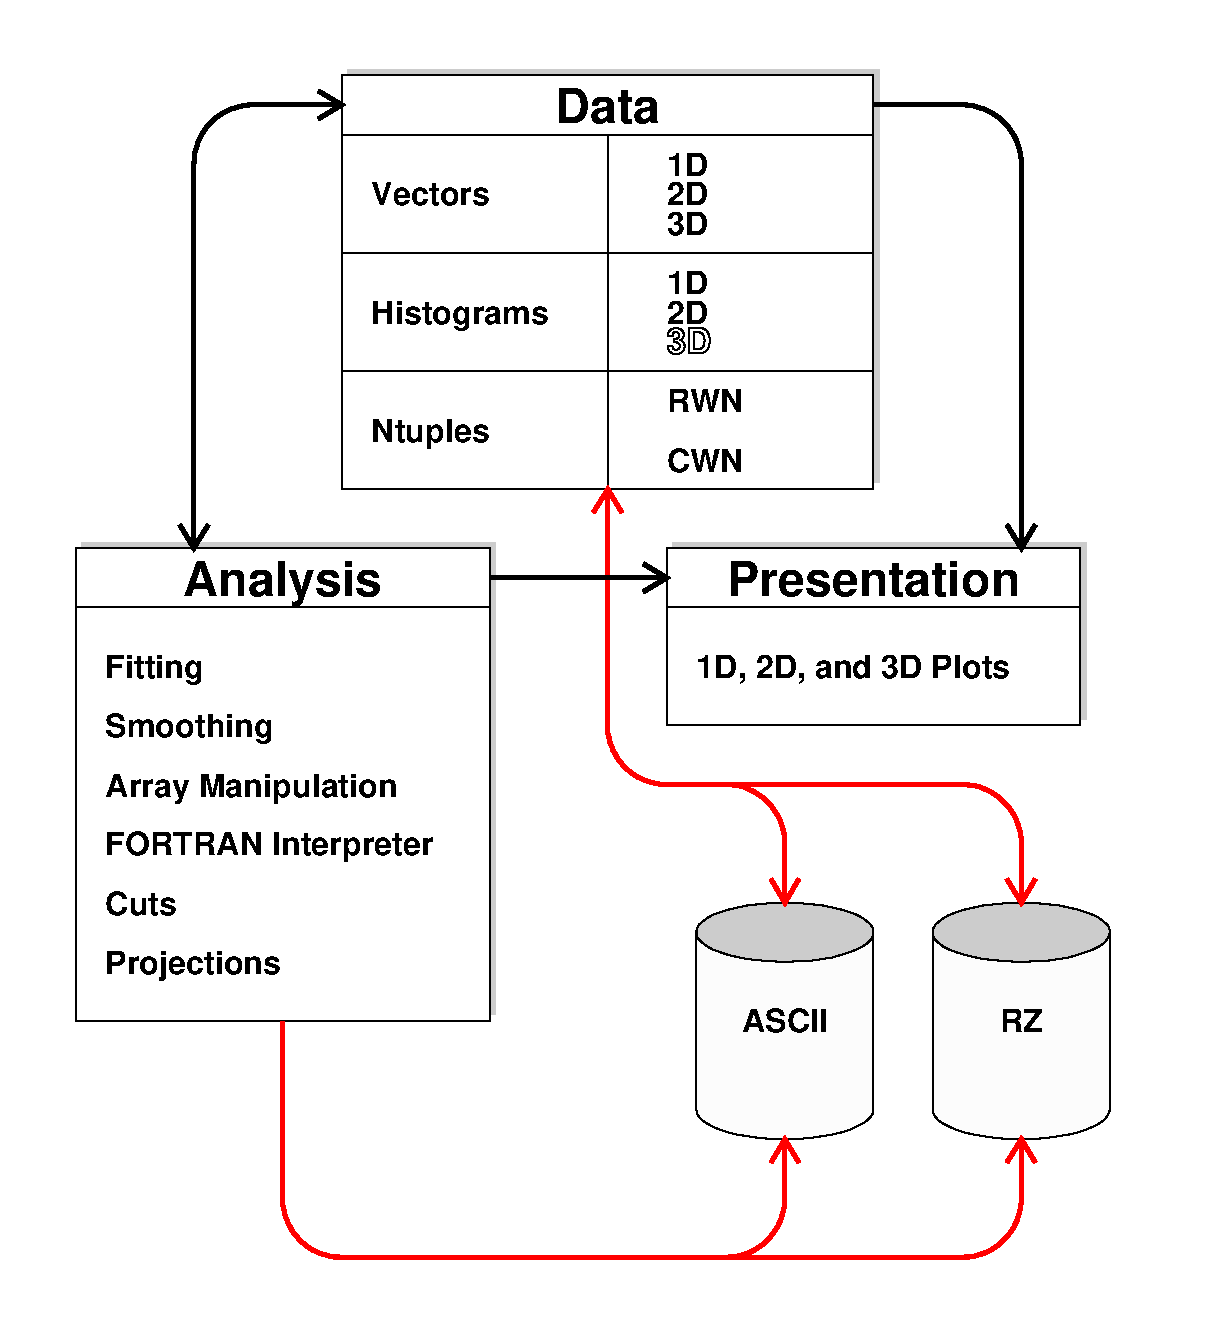
\epsfig{file=pawtut01.eps,height=.5\linewidth}}
\end{center}
\caption{PAW's fundamental ``data'' objects}
\label{fig:pawobjects}
\end{figure}

\subsection*{Objects:}

\begin{itemize}
\item {\bf 1D Histograms.}  
\index{histogram}
\index{histogram!1D}
      A histogram is the basic statistical analysis tool of PAW. Histograms are
      created (``booked'') by choosing the basic characteristics of their bins,
      variables, and perhaps customized display parameters; numbers are entered
      into the histogram bins from an Ntuple (the histogram is ``filled'') by 
      selecting the desired events, weights, and variable transformations to be
      used while counts are accumulated in the bins. Functional forms are 
      frequently fit to the resulting histograms and stored with them. Thus a 
      fit as an object is normally associated directly with a histogram, 
      although it may be considered separately.
\item {\bf 2D Histograms.}  
\index{histogram!2D}
      2D (and higher-dimensional) histograms are logical generalizations of 1D
      histograms. 2D histograms, for example, are viewable as the result of 
      counting the points in a the sections of a rectangular grid overlaid on 
      a scatter plot of two variables. Higher-dimensional histograms can also 
      be fitted, and support for associating the results of a fit to a 
      higher-dimensional histogram is currently being incorporated in PAW.
\item {\bf Ntuples.}  
\index{Ntuple}
      An Ntuple is the basic type of data used in PAW. It consists of a list of
      identical data structures, one for each event. Typically, an Ntuple is 
      made available to PAW by opening a HBOOK file; this file, as created by 
      HBOOK, contains one or more Ntuples and possibly also directories, which
      may store a hierarchy of Ntuples and histograms. A storage area for an 
      Ntuple may be created directly using \Ucom{NTUPLE/CREATE}; data may then
      be stored in the allocated space using the \Ucom{NTUPLE/LOOP} or 
     \Ucom{NTUPLE/READ} commands. Other commands merge Ntuples into larger 
      Ntuples, project vector functions of the Ntuple variables into histograms,
      and plot selected subsets of events.
\item {\bf Cuts.}  
\index{cut}
      A cut is a Boolean function of Ntuple variables. Cuts are used to select
      subsets of events in an Ntuple when creating histograms and ploting 
      variables.
\item {\bf Masks.}  
\index{mask}
      Masks are separate files that are logically identical to a set of boolean 
      variables added on the end of an Ntuple's data structure. A mask is 
      constructed using the Boolean result of applying a cut to an event set.
      A mask is useful only for efficiency; the effect of a mask is identical 
      to that of the cut that produced it.
\item {\bf Vectors.}  
\index{vector}
      PAW provides the facilities to store vectors of integer or real data. 
      These vectors, or rather arrays with up to 3 index dimensions, can be 
      manipulated with a set of dedicated commands. Furthermore they are 
      interfaced to the array manipulation package SIGMA and to the Fortran 
      interpreter COMIS. They provide a convenient and easy way to analyse 
      small data sets stored in ASCII files.
\item {\bf PostScript (meta)files.}  
\index{metafile}
      PostScript format (meta)files are especially useful because they can be 
      directly printed on most printers; furthermore, the printed quality of 
      graphics objects such as fonts can be of much higher quality than the 
      original screen image.
\item {\bf Pictures.}  
\index{picture}
      A {\it picture\/} is an exact copy of the screen image, and so its
      storage and redisplay time are independent of complexity. Pictures are 
      also intensively used for object picking in the Motif version of PAW.
\item {\bf ZEBRA(RZ) Logical Directories.}  
\index{directory!ZEBRA}
      In a single PAW session, the user may work simultaneously with many 
      Ntuples, histograms, and hierarchies of Ntuple and histograms. However, 
      this is not accomplished using the native operating system's file handler.
      Instead, the user works with a set of objects that are {\it similar\/} to
      a file system, but are instead managed by the ZEBRA RZ package. This can
      be somewhat confusing because a single operating system file created by 
      RZ can contain an entire hierarchy of ZEBRA logical directories; 
      furthermore, sections of internal memory can also be organized as ZEBRA 
      logical directories to receive newly-created PAW objects that are not 
      written to files. A set of commands \Ucom{CDIR}, \Ucom{LDIR}, and 
      \Ucom{MDIR} are the basic utilities for walking through a set of ZEBRA 
      logical directories of PAW objects; Each set of directories contained in
      an actual file corresponds to a logical unit number, and the root of the
      tree is usually of the form \texttt{//LUNx};  the PAW objects and logical
      directories stored in internal memory have the root \texttt{//PAWC}.
\index{Macros}
\index{macro}
      A macro is a set of command lines stored in a file, which can be created 
      or modified with any text editor. In addition to all the PAW commands, 
      special macro flow control statements are also available.
\item {\bf Operating System File Directories.}  
\index{operating system}
      Many different ZEBRA files, some with logically equivalent Ntuples and 
      histograms, can be arranged in the user's operating system file 
      directories. Thus one must also keep clearly in mind the operating system
      file directories and their correspondence to the ZEBRA logical directories
      containing data that one wishes to work with.  In many ways, the operating
      system file system is also a type of ``object'' that forms an essential 
      part of the user's mental picture of the system.
\end{itemize}
 

\begin{figure}
\centering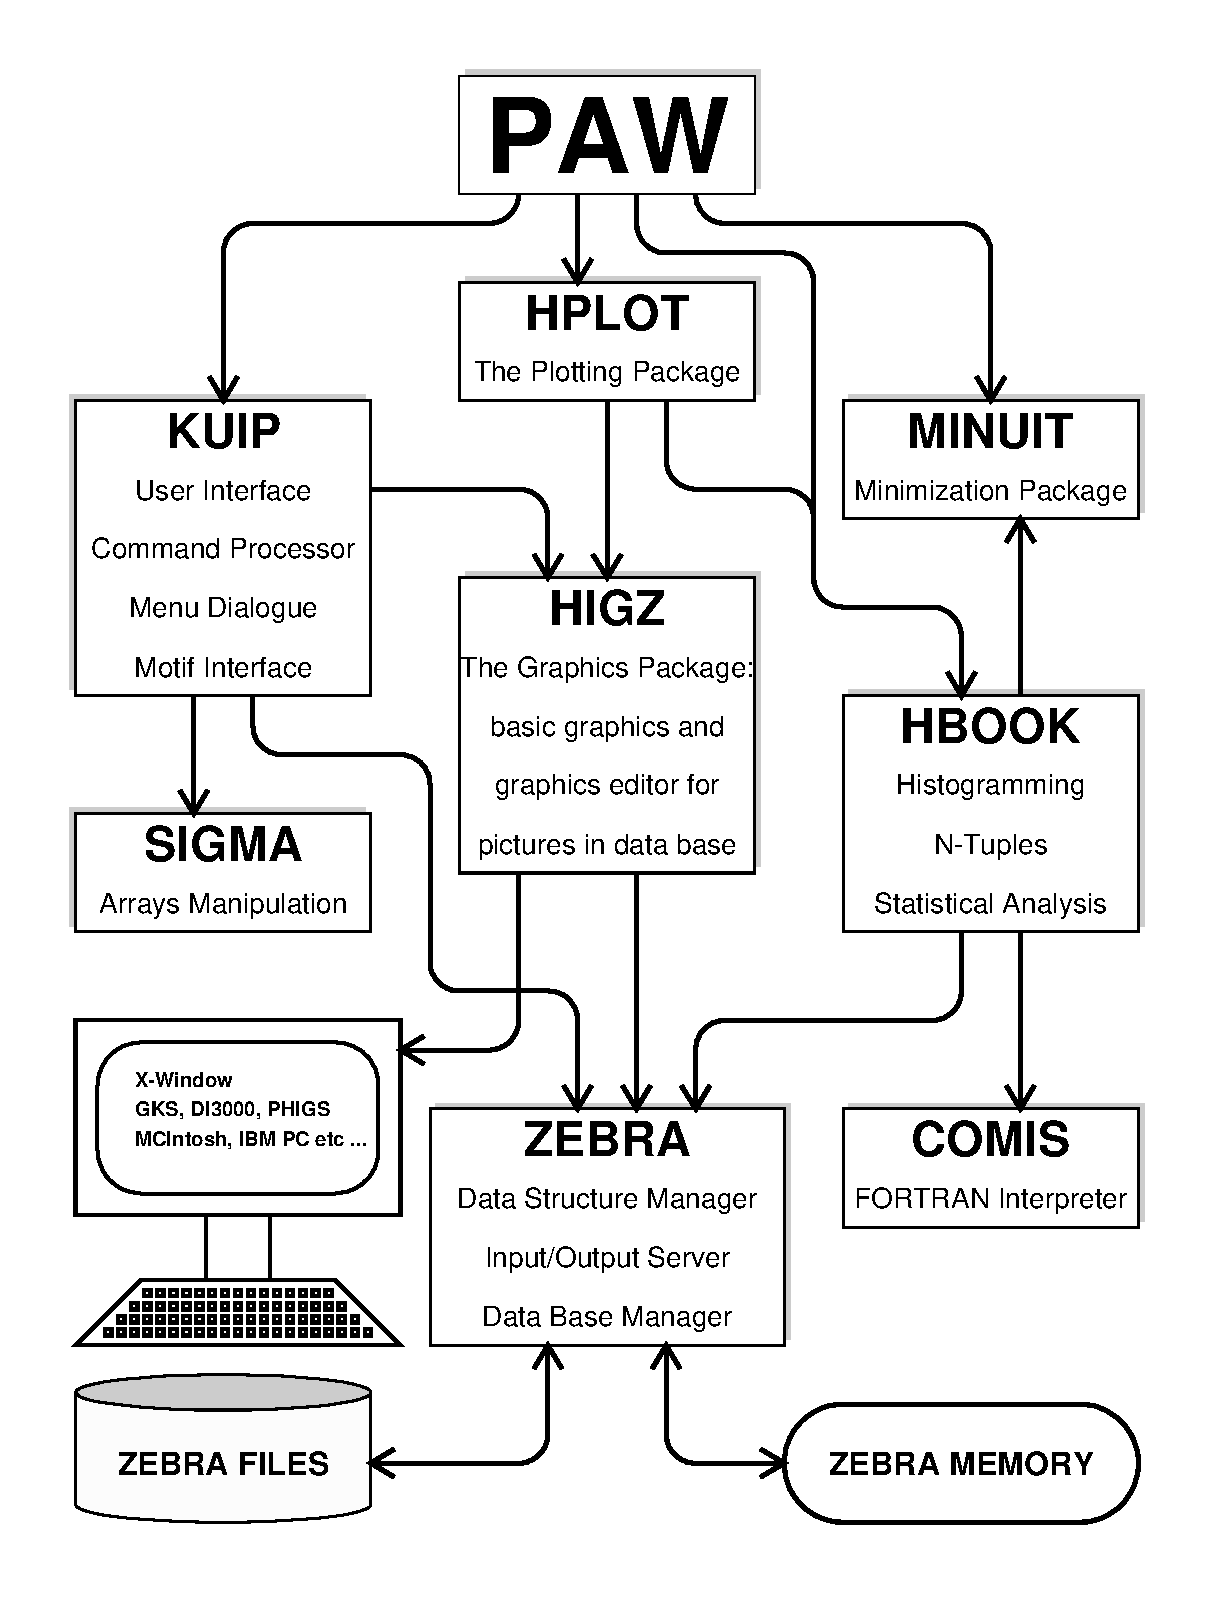
\includegraphics[width=.5\textwidth]{pawtut00.eps}
\caption{PAW and its components}
\label{fig:PAWcomp}
\end{figure}

\section{The Component Subsystems of PAW}
\label{sec:pawstructure}
\index{structure of PAW}
\index{PAW!structure}

The PAW system combines different tools and packages, which
can also be used independently and some of which have already
a long history behind them (e.g. HBOOK and
HPLOT, SIGMA, COMIS, MINUIT).
Figure \ref{fig:PAWcomp} shows the various components of PAW.
\index{components!of PAW}

\subsection{KUIP - The user interface package}
\index{KUIP}
\index{command!definition file (CDF)}
\index{CDF Command Definition File}
\index{alias}
\index{abbreviation}
\index{macro}
\index{dialogue style}
\index{default setting}
\index{history file}
 
The purpose of KUIP
({\bf K}it for a {\bf U}ser
{\bf I}nterface {\bf P}ackage) is to handle
the dialogue between the user and the application program (PAW
in our case). It
parses the commands input into the system, verifies them for
correctness and then hands over control to the relevant action
routines.
 
\index{command!abbreviation}
Commands are grouped in a tree structure and they can be
{\bf abbreviated} to their shortest unambiguous
form. If an ambiguous command is typed, then KUIP responds by showing
all the possibilities.
\index{alias}
{\bf Aliases} allow the user to abbreviate part or the whole
of commonly used command and parameters.
A sequence of PAW commands can be stored in a text file and, combined
with flow control statements, form a powerful {\bf macro} facility.
\index{macro!parameter}
\index{parameter}
With the help of {\bf parameters},
whose values can be passed to the macros, general and adaptable
task solving procedures can be developed.
 
\index{style of dialogue}
\index{dialogue!style}
 The user has the choice between different dialogue styles ranging from
the conventional command line interface to a high-level windowed environment
based on OSF/Motif \index{Motif}.
In order to save typing, {\bf default values},
providing reasonable settings, can be used for most
\index{history file}
parameters of a command. A {\bf history file},
containing the {\tt\underline{n}} most recently entered
commands, is automatically kept by KUIP
and can be inspected, copied or re-entered at any time.
The history file of the last PAW session is also kept on disk.

\subsection{HBOOK and HPLOT - The histograming and plotting packages}
\index{HBOOK}
\index{HPLOT}

HBOOK and its graphics interface
HPLOT are libraries of FORTRAN callable
subroutines which have been
in use for many years.
They provide the following functionality:

\begin{UL}
\item One- and two-dimensional histograms and Ntuples
\item Projections and slices of two-dimensional histograms and Ntuples
\item Complete control (input and output) of the histogram contents
\item Operations and comparison of histograms
\item Minimization and parameterization tools
\item Random number generation
\item Histograms and Ntuples structured in memory (directories)
\item Histograms and Ntuples saved onto direct access ZEBRA files
\item Wide range of graphics options:
\begin{UL}
\item Contour histograms, bar chart, shaded histograms, error bars, colour
\item Smoothed curves and surfaces
\item Scatter, lego, contour and surface plots
\item Automatic windowing
\item Graphics input
\end{UL}
\end{UL}

\subsection{HIGZ - The graphics interface package}
\index{HIGZ}

A {\bf H}igh level
{\bf I}nterface to {\bf G}raphics and {\bf Z}EBRA
(HIGZ) has been developed within the PAW project. This package is
a layer between the application program (e.g. PAW/HPLOT) and the basic
graphics package (e.g. X11) on a given system. Its basic aims are:

\begin{UL}
\item Full transportability of the picture data base.
\item Easy manipulation of the picture elements.
\item Compactness of the data to be transported and accessibility
      of the pictures in direct access mode.
\item Independence of the underlying basic graphics package.
      Presently HIGZ is interfaced with several GKS packages,
      X- Windows (X11), PHIGS, Mac, PC's graphic systems, 
      GL (Silicon Graphics), GDDM (IBM),
      GPR (Apollo) as well as with the DI3000 system. Note that some of these
      graphics systems are now obsolete. PAW is now mainly used in its X11 
      version.
\index{GKS}
\index{X windows}
\index{GL (Silicon Graphics)}
\index{GPR (Apollo)}
\index{GMR3D (Apollo)}
\index{GDDM (IBM)}
\index{DI3000}
\end{UL}

These requirements have been incorporated into HIGZ by exploiting
the data management system ZEBRA.
 
HIGZ does not introduce new basic graphics features, but introduces
some macroprimitives for frequently used functions
(e.g. arcs, axes, boxes, pie-charts, tables). The system
provides the following features:

\begin{UL}
\item Basic graphics functions: basic primitives, attributes, space definition.
\item Higher-level macroprimitives.
\item Data structure management using an interface to the ZEBRA system.
\item Interactive picture editing.
\end{UL}

These features, which are available simultaneously, are
particularly useful during
an interactive session, as the user is able to
``replay'' and edit previously created pictures, without the need to re-run
\index{replay}
the application program. 
A direct interface to PostScript is also
available.

\subsection{ZEBRA - The data structure management system}
\index{ZEBRA}

The data structure management package ZEBRA
was developed at CERN in order to overcome the lack of dynamic
data structure facilities in FORTRAN, the favourite computer language
in high energy physics. It implements the {\bf dynamic
creation and modification} of data structures at execution time
and their transport
to and from external media on the same or different computers, memory
to memory, to disk or over the network, at an
{\bf insignificant cost} in terms of execution-time overheads.
 
\index{input/output}
\index{native input/output}
\index{exchange input/output}
\index{RZ file}
ZEBRA manages any type of structure, but specifically
supports linear structures (lists) and trees.
ZEBRA input/output is either of a sequential or direct access type.
Two data representations,
{\bf native} (no data conversion when transferred to/from the
external medium) and {\bf exchange} (a conversion to an
interchange format is made), allow data to be transported between
computers of the same and of different architectures.
The direct access package {\bf RZ} can be used
to manage hierarchical data bases. In PAW this facility is exploited
to store histograms, Ntuples and pictures in a hierarchical direct access
directory structure.

\subsection{MINUIT - Function minimization and error analysis}
\index{MINUIT}
\index{fit}
\index{statistic!analysis}
\index{minimisation}
\index{chisquare}
\index{correlation}
 
MINUIT is a tool to find the {\bf minima of a
multi-parameter function} and
analyse the {\bf shape around the minimum}. It can be used for
{\bf statistical analysis} of
curve fitting, working on a \(\chi^2\) or log-likelihood function,
to compute the {\bf best fit} parameter values, their uncertainties and
correlations. {\bf Guidance} can be provided in order to find the
correct solution, parameters can be kept fixed and data points
can be easily added or removed from the fit. An interactive Motif based
interface is in preparation.

\subsection{COMIS - The FORTRAN interpreter}
\index{COMIS}

The COMIS interpreter allows the user to execute interactively
a set of FORTRAN routines in interpretive mode.
The interpreter implements a large subset of the complete FORTRAN
language. It is an extremely important tool because
it allows the user
to specify his own complex data analysis procedures, for example
selection criteria or a minimisation function.

\subsection{SIGMA - The array manipulation language}
\index{SIGMA}

A scientific computing programming language SIGMA
({\bf S}ystem for {\bf I}nteractive
{\bf G}raphical {\bf M}athe\-ma\-tical
{\bf A}pplications),
which was designed essentially for mathematicians and
theoretical physicists is integrated into PAW.  Its main characteristics are:

\begin{UL}
\item The basic data units are scalars and one or more dimensional
      rectangular arrays, which are automatically handled.
\item The computational operators resemble those of FORTRAN.
\end{UL}

\section{A PAW Glossary}

\subsection*{Data Analysis Terminology}


\begin{DL}{MMMMM}
\item[DST]       A ``Data Summary Tape'' is one basic form of  output from
                 a typical physics experiment.  A DST is generally not used
                 directly by PAW, but is analyzed by customized user programs
                 to produce Ntuple files, which PAW can read directly.
\index{DST}
\index{DST!Data Summary Tape}
\item[Ntuple]    A list of identical data structures, each typically 
                 corresponding to a single experimental event. The data 
                 structures
                 themselves frequently consist of a row of numbers, so that
                 many Ntuples may be viewed as
                 two-dimensional arrays of data variables, with one
                 index of the array describing the position of the data
                 structure in the list (i.e., the row or event number),
                 and the other index referring to the position of the data
                 variable in the row (i.e., the column or variable number).
                 A meaningful name is customarily assigned to each column
                 that describes the variable contained in that column for each
                 event.  
\index{Ntuple}
\item[Event]     A single instance of a set of data  or experimental measurements,
                 usually consisting of a sequence of variables or structures of
                 variables resulting from a partial analysis of the raw data.
                 In PAW applications, one typically examines the statistical
                 characteristics of large sequences of similar events.
\index{event}
\item[Variable]  One of a user-defined set of named values associated with a single
                 event in an Ntuple.
                 For example,
                 the \((x,\,y,\,z)\) values of a momentum vector could each
                 be variables for a given event.  Variables are typically
                 useful experimental quantities that are stored in an
                 Ntuple;  they are used in algebraic formulas
                 to define boolean cut criteria
                 or other dependent variables that are
                 relevant to the analysis.
\item[Cut]       A  boolean-valued function of the variables of a given event.
                 Such functions allow the user to specify that only  events
                 meeting certain criteria are to be included in a given distribution.
\index{cut}
\item[Mask]      A set of columns of zeros and ones that is identical in form
                 to a new set of Ntuple variables.  A mask is typically
                 used to save the results of applying a set of cuts to a large
                 set of events so that
                 time-consuming selection computations are not repeated needlessly.
\index{mask}
\item[Function]  Sequence of one or more statements with a FORTRAN-like syntax
                 entered on the command line or via an external file.
\index{function}
\end{DL}

\subsection*{Statistical Analysis Terminology}

\begin{DL}{MMMMM}
\item[Histogram] A one- or two-dimensional array of data, generated
                 by HBOOK in batch or in a PAW session. Histograms are (implicitly or
                 explicitly) declared (booked);
                 they can be filled by explicit entry of data
                 or can be derived from other histograms. The information stored
                 with a histogram includes a title, binning and packing definitions,
                 bin contents and errors, statistic values, possibly an
                 associated function vector, and output attributes.
                 Some of these items are optional.
                 The ensemble of this information constitutes an {\bf histogram}.
\index{histogram}
\index{histogram!booking}
\item[Booking]   The operation of declaring (creating) an histogram.
\index{book histogram}
\item[Filling]   The operation of entering data values into a given histogram.
\index{fill!histogram}
\index{histogram!filling}
\item[Fitting]   Least squares and maximum likelihood fits of
                 parametric functions to histograms and vectors.
\index{fit}
\item[Projection]The operation of projecting two-dimensional
                 distributions onto either or both axes.
\index{projection}
\item[Band]      A band is a projection onto the X (or Y) axis
                 restricted to an interval
                 along the other Y (or X) axis.
\index{band}
\item[Slice]     A slice is a projection onto the X (or Y) 
                 axis restricted to one bin
                 along the other Y (or X) axis.
                 Hence a slice is a special case of a band, with
                 the interval limited to one bin.
\index{slice}
\item[Weight]    PAW allows the user to include a
                 multiplicative statistical bias for each event which is a scalar
                 function of the available variables.  This permits the user to
                 correct for known statistical biases in the data when making
                 histograms of event distributions.
\end{DL}

\subsection*{KUIP/ZEBRA User Environment Terminology}

\begin{DL}{MMMMM}
\item[Macro]     A text file containing a set commands 
                 and logical constructs to control the flow of execution. 
                 Parameters can be supplied when calling a macro.
\index{macro}
\item[Vector]    The equivalent of a FORTRAN array supporting 
                 up to three dimensions.
                 The elements of a vector can be stored using a real or an
                 integer representation;
                 they can be entered interactively on a terminal or read
                 from an external file.
\index{vector}
\item[Logical Directory\ ]
                 The ZEBRA data storage system resembles a file system organized
                 as logical directories.  PAW maintains
                 a global variable corresponding to the ``current directory'' where
                 PAW applications will look for PAW objects such as histograms.
                 The ZEBRA directory structure is a tree, and user functions permit
                 the ``current directory'' to be set anywhere in the current tree,
                 as well as creating new ``directories'' where the results
                 of PAW actions can be stored.  A special
                 directory called \texttt{//PAWC} corresponds to a memory-resident
                 branch of this virtual file system.  ZEBRA files may be written
                 to the operating system file system, but entire hierarchies of
                 ZEBRA directories typically are contained in a single binary operating
                 system file.
\end{DL}

\subsection*{Graphics Production Terminology}

\begin{DL}{MMMMM}
\item[Metafile]  A file containing graphical information
                 stored in a device independent format,
                 which can be replayed on various types of output devices.
                 (e.g. PostScript).
\index{metafile}
\item[Picture]   A graphics object composed of graphics primitives 
                 and attributes.
                 Pictures are generated by
                 the HIGZ graphics interface and they can be stored in a picture
                 direct-access database, built with the RZ-package of the
                 data structure manager ZEBRA.
\index{picture}
\index{PostScript}
\item[PostScript]
                 A high level page description language permitting the description of complex
                 text and graphics using only text commands.  Using PostScript
                 representations of graphics makes it possible to create graphics
                 files that can be exchanged with other users and printed on
                 a wide variety of printers without regard to the computer system
                 upon which the graphics were produced.  Any graphics display
                 produced by PAW can be expressed in terms of PostScript, written
                 to a file, and printed.
\end{DL}
 
\endinput

%%%%%%%%%%%%%%%%%%%%%%%%%%%%%%%%%%%%%%%%%%%%%%%%%%%%%%%%%%%%%%%%%%%%%%%%%%%%%%%%
%                                                                              %
%   PAW   - Reference Manual -- LaTeX Source                                   %
%                                                                              %
%   Chapter 2: General principles                                              %
%                                                                              %
%   EPS file      : pawtut02.eps                                               %
%                   pawppoverview1.eps                                         %
%                   pawppoverview2.eps                                         %
%                   pawtut10.eps                                               %
%                                                                              %
%   Editor: Michel Goossens / IT-ASD                                           %
%   Last Mod.: 30 July 1998 Olivier Couet                                      %
%                                                                              %
%%%%%%%%%%%%%%%%%%%%%%%%%%%%%%%%%%%%%%%%%%%%%%%%%%%%%%%%%%%%%%%%%%%%%%%%%%%%%%%%

\chapter{General principles}
\label{sec:PRINCIP}
\newcommand{\RZ}{{\sf RZ}\index{RZ}}
\newcommand{\PHIGS}{{\sf PHIGS}\index{PHIGS}}
\newcommand{\GPHIGS}{{\sf GPHIGS}\index{GPHIGS}}
\newcommand{\XPAW}{{\sf PAW}\index{PAW (Physics Analysis Workstation)}}
\newcommand{\PS}{{\sf Post\-Script}\index{PostScript}}
\newcommand{\EPS}{{\sf En\-cap\-su\-la\-ted Post\-Script}\index{PostScript!Encapsulated}}
\newcommand{\FALCO}{{\sf FALCO}\index{FALCO}}
\newcommand{\MSDOS}{{\sf MSDOS}\index{MSDOS}}
\newcommand{\MAC}{{\sf MacIntosh}\index{MacIntosh}}
\newcommand{\GDDM}{{\sf GDDM}\index{GDDM}}
\newcommand{\XW}{{\sf X Window System}\index{X Window System}}
\newcommand{\Xxi}{{\sf X11}\index{X11}}
\newcommand{\GL}{{\sf GL}\index{GL}}
\newcommand{\GPR}{{\sf GPR}\index{GPR}}
\newcommand{\GMR}{{\sf GMR}\index{GMR}}
\newcommand{\MOTIF}{{\sf Motif}\index{Motif}}
\newcommand{\XLIB}{{\sf Xlib}\index{Xlib}}

\newcommand{\NDC}{normalized device coordinates\index{coordinates!normalized device}}
\newcommand{\DC}{device coordinates\index{coordinates!device}}
\newcommand{\WC}{world coordinates\index{coordinates!world}}

\newcommand{\ndc}{{\sf NDC}\index{coordinates!normalized device}}
\newcommand{\dc}{{\sf DC}\index{coordinates!device}}
\newcommand{\wc}{{\sf WC}\index{coordinates!world}}

\newcommand{\FORTRAN}{{\sf Fortran}\index{Fortran}}
\newcommand{\CHARACTER}{{\tt CHARACTER}}

\newcommand{\UGP}{underlying graphics package\index{underlying graphics package}}
\newcommand{\UGPs}{underlying graphics packages\index{underlying graphics package}}

\newcommand{\HW}{{\tt higz\_windows.dat}\index{higzwindows.dat}}

\newcommand{\nt}{{\sf NT}\index{normalization transformation}}
\newcommand{\wt}{{\sf WT}\index{workstation transformation}}

\newcommand{\NT}{normalization transformation\index{normalization transformation}}
\newcommand{\NTs}{normalization transformations\index{normalization transformation}}
\newcommand{\WT}{workstation transformation\index{workstation transformation}}
\newcommand{\WTs}{workstation transformations\index{workstation transformation}}
\newcommand{\ASCII}{{\tt ASCII}\index{ASCII}}

\newcommand{\UNIX}{{\sf UNIX}\index{UNIX}}
\newcommand{\VMS}{{\sf VAX/VMS}\index{VAX/VMS}}

\newcommand{\MB}{{\bf Main Browser}\index{Main Browser}}
\newcommand{\EW}{{\bf Executive Window}\index{Executive Window}}
\newcommand{\TP}{{\bf Transcript Pad}\index{Transcript Pad}}
\newcommand{\IP}{{\bf Input Pad}\index{Input Pad}}
\newcommand{\NV}{{\bf Ntuple Viewer}\index{Ntuple Viewer}}
\newcommand{\HSP}{{\bf Histogram Style Panel}\index{Histogram Style Panel}}
\newcommand{\PL}{{\bf PAW++ Locate}\index{PAW++ Locate}}
\newcommand{\GW}{{\bf Graphics Window}\index{Graphics Window}}
\newcommand{\CE}{{\bf Cut Editor}\index{Cut Editor}}

\section{Access to PAW}
\label{sec:PACCESS}\index{PAW!access}
 
At CERN the PAW program
is interfaced on all systems via a command
procedure which gives access to the three release levels of
the CERN Program Library
(\texttt{PRO}duction, \texttt{OLD} and the \texttt{NEW} areas) and
sets the proper environment if necessary.
Users who are not at CERN or who are using non-central
computer systems should contact their system
administrator for help on PAW.
\index{CERN Program Library!OLD}
\index{CERN Program Library!NEW}
\index{CERN Program Library!PRO}

\subsection{VAX/VMS}
\index{VAX}
\index{VMS}
 
A command file \texttt{CERN_ROOT:\lsb EXE\rsb PAW.COM}
is defined system-wide via the logical
symbol \texttt{PAW}; its interface is:

\begin{alltt}
      \Ucom{PAW/ver}\rmfamily\qquad(the default is \texttt{PRO})
\end{alltt}

You may set the initialization of PAW either as a \texttt{PAWLOGON.KUMAC}
located in your home directory, or through the
logical symbol \texttt{DEFINE PAW\$LOGON disk:\lsb user.subdir\rsb file.kumac}
to be defined usually in your \texttt{LOGIN.COM}.

\subsection{Unix systems}
\index{Apollo}
\index{unix}
 
The driver shell script is located in the file
\texttt{/cern/pro/bin/paw}.
In order to access it automatically you could add the
directory \texttt{/cern/pro/bin} to your command search path.
\index{path}%
\index{command!search path}%
\index{HELP}%
\index{X windows}%
\index{X11}%
\index{display}%
\index{host}%
\index{workstation}%
\index{Domain}%
\index{version}%
\index{PAWLOGON}%
The command syntax is:
\begin{alltt}
      \Ucom{paw -v ver}\rmfamily\qquad(the default is \texttt{-v PRO})
\end{alltt}

\subsection{Workstation type}
 
PAW needs to know the X-host where graphics must be
displayed; this can be specified on each system on the command line:
\begin{alltt}
      Vax/VMS:   \Ucom{PAW/X11/host=yourhost}
      Unix:      \Ucom{paw -d X11 -h yourhost}
\end{alltt}
or at the ``\texttt{Workstation}'' prompt in PAW:
\texttt{Workstation type (?=HELP) \lsb CR\rsb =1 : \Ucom{1.yourhost}}
 
If \texttt{yourhost} is not specified, the output is redirected (like for all
X11 applications) to the display defined via the environment variable 
{\tt DISPLAY}.

The workstation type selects which type of workstation has to be opened. 
It corresponds to a line number in a file \texttt{higz_windows.dat}.
PAW tries to open this file in your current working directory.
If it does not succeed it tries in your HOME directory.
If it doesn't succeed once more, it creates the file in your HOME directory 
as follows:
\begin{verbatim}
                      0000 0000 0600 0600
                              .
                              .
                              .
                      0000 0000 0600 0600
\end{verbatim}
where the lines define each of the workstation types (from 1 to 10) with
the x-margin (left), y-margin (top), x-size (width) and y-size (height) of the
corresponding window in pixels.

For a more complete and up to date description you can refer to the PAW FAQs 
avaialable from the PAW web home page.

\subsection{Different modes to start PAW}

\begin{UL}
\index{batch}
\item A {\bf batch} version of PAW is available 
      (note that batch implies workstation type \texttt{0}):
\begin{alltt}
 On Unix   do:  \Ucom{paw -b macroname}
 On VMS    do:  \Ucom{PAW/BATCH=macroname}
\end{alltt}
\index{PAWLOGON}
\item One can {\bf disable} the automatic execution 
      of the \texttt{PAWLOGON} macro:
\begin{alltt}
 On Unix   do:  \Ucom{paw -n}
 On VMS    do:  \Ucom{PAW/NOLOG}
\end{alltt}
\end{UL}

\section{Initialising PAW}
\label{sec:INITIAL}
\index{PAW!initialisation}
 
When PAW is started, a {\bf system} startup
procedure is initiated, which indicates the current
version of PAW and requests the {\bf workstation type} of
the terminal or workstation which you are using.
\index{initialisation}
\index{workstation!type}
\begin{alltt}
\$ \Ucom{PAW}
 ******************************************************
 *                                                    *
 *            W E L C O M E    to   P A W             *
 *                                                    *
 *        Version 2.10/01       2 September 1998      *
 *                                                    *
 ******************************************************
 Workstation type (?=HELP) <CR>=1 : ?

 List of valid workstation types:
       0:  Alphanumeric terminal
    1-10:  Describe in file higz_windows.dat
  n.host:  Open the display on host (1 < n < 10)
    7878:  FALCO terminal
    7879:  xterm
\end{alltt}
Note that if you specify {\Ucom{0}},
PAW will not open a graphics workstation.
This may be appropriate if one wants to use PAW on an alphanumeric
terminal.
 
Before passing control to the user, the system looks for a user-supplied file
\texttt{pawlogon.kumac}.
The latter can contain
commands which the user wants to be executed at PAW startup, e.g.
declaration of files, creation of aliases, definition of HPLOT parameters.
\index{PAWLOGON}
A simple version of this PAW initialisation file, displaying date
and time, can be:

\begin{alltt}
mess '******************************************************'
mess '*                                                    *'
mess '*   Starting PAW session on '//$date//' at '//$time//'     *'
mess '*                                                    *'
mess '******************************************************'
\end{alltt}
 
In order to
only have one version of this file on VAX/VMS the user should define
a {\bf logical name} \texttt{PAW\$LOGON} in his
\texttt{LOGIN.COM},
as explained on the previous page.
The file \texttt{pawlogon.kumac} is taken in the current directory.

\section{Command structure}
\label{sec:COMSTRU}
\index{command!structure}
 
PAW is based on the KUIP\cite{bib-KUIP} User Interface package,
which can provide different types of dialogue styles:

\begin{UL}
\item Command mode,
      where the user enters a command line via the terminal keyboard.
\item Alphanumeric menu mode,
      where the command is selected from a list.
\item Graphics menu modes:\\
\index{menu}
\hspace*{1em}$\bullet$ 
Pull-down menus, fixed layout reflecting the command structure;\\
\index{pull-down menu}
\hspace*{1em}$\bullet$ 
Panels of function keys, interactive user definable multiple layouts.
\index{panel!menu}
\end{UL}

It is possible to change interactively from one style to another.
 
The general format of a PAW command line is:
\begin{alltt}
      \Ucom{command parameters}
\end{alltt}
The first part of the {\bf command} has the format:
\begin{alltt}
      \Ucom{object/verb}
\end{alltt}
where the {\bf object} is the item on which the action is performed
(e.g. \texttt{HISTOGRAM, VECTOR, NTUPLE})
and the \texttt{verb} is the action to be performed (e.g.
\texttt{CREATE, DELETE, PLOT}). 
In some cases the object needs to be
specified further (e.g. \Ucom{GRAPHICS/PRIMITIVE}),
while in other cases the verb's action needs to be clarified further
(e.g. \Ucom{CREATE/1D}).
\index{abbreviation}
\index{command!abbreviation}
All components can be {\bf abbreviated} to their shortest unambiguous form. 
For example the two following
lines will have the same effect of creating a vector \texttt{A} with
nine components:
\begin{alltt}
     \Ucom{VECTOR/CREATE A(9)}
{\rm or}
     \Ucom{VE/CR A(9)}
\end{alltt}
\index{command!parameter!mandatory}
\index{command!parameter!optional}
In the case that the form is ambiguous all possible interpretations
for the given abbreviation are displayed.
 
The second part of a command are its {\bf parameters} and their meaning
is determined by their {\bf position}.
\index{mandatory parameter}
\index{optional parameter}
Some of these can be {\bf mandatory}
with the remaining ones {\bf optional}.
If all mandatory parameters are not provided on the command line,
PAW will prompt the user to specify them, indicating
the default values if defined.
If the user wants
to assign the default value to a parameter from the command line
he can use the {\bf place-holder} character
{\bf exclamation mark (!)} to signify this to PAW.
\index{place-holder!exclamation mark character}
\index{exclamation mark character!place-holder}
In the case of optional parameters, the user {\bf must} provide them
in the correct sequence if he wants to {\bf change} their values,
otherwise the corresponding defaults are taken.
Parameters containing blanks must be enclosed within single quotes.
 
In the example below we create a one-dimensional histogram,
providing the parameters one by one answering the PAW query:
\begin{alltt}
      PAW > \Ucom{histogram/create/1dhisto}
      Histogram Identifier (<CR>= ): \Ucom{10}
      Histogram title (<CR>= ): \Ucom{title1}
      Number of channels (<CR>=100): \Ucom{<CR>}
      Low edge (<CR>=0): \Ucom{10.}
      Upper edge (<CR>=100): \Ucom{20.}
\end{alltt}
For the command below
we provide all parameters on the command line, including
an optional one (\texttt{1000.}),
which by default has the value \texttt{0}.
Note that this parameter {\bf must} be specified
explicitly, since PAW {\bf does not} prompt for it,
as seen in the previous example.
Note also the use of the exclamation mark to take the default for the
number of channels (\texttt{100}).
\begin{alltt}
      PAW > \Ucom{hi/cr/1d 20 title2 ! 10. 20. 1000.}
\end{alltt}

\section{Getting help}
\label{sec:GETHELP}
 
Once inside PAW, one can start entering commands.
An interesting first try would be the \Ucom{HELP} command,
\index{HELP}
which displays a list of items, preceded by a number
and followed by one line of explanation.
In the next example we search for a command to
create a one-dimensional histogram.
\begin{falltt}
      PAW > \Ucom{help}
 
From  /...

 1:   KUIP          Command Processor commands.
 2:   MACRO         Macro Processor commands.
 3:   VECTOR        Vector Processor commands.
 4:   HISTOGRAM     Manipulation of histograms, Ntuples.
 5:   FUNCTION      Operations with Functions. Creation and plotting.
 6:   NTUPLE        Ntuple creation and related operations.
 7:   GRAPHICS      Interface to the graphics packages HPLOT and HIGZ.
 8:   PICTURE       Creation and manipulation of HIGZ pictures.
 9:   ZEBRA         Interfaces to the ZEBRA RZ, FZ and DZ packages.
10:   FORTRAN       Interface to MINUIT, COMIS, SIGMA and FORTRAN
                    Input/Output.
11:   NETWORK       To access files on remote computers.
12:   OBSOLETE      Obsolete commands.

Enter a number ('Q'=command mode): \Ucom{4} 

   /HISTOGRAM

   Manipulation of histograms, Ntuples.  Interface to the HBOOK package.


From  /HISTOGRAM/...

 1: * FILE          Open an HBOOK direct access file.
 2: * LIST          List histograms and Ntuples in the current directory.
 3: * DELETE        Delete histogram/Ntuple ID in Current Directory
                    (memory).
 4: * PLOT          Plot a single histogram or a 2-Dim projection.
 5: * ZOOM          Plot a single histogram between channels ICMIN and
                    ICMAX.
 6: * MANY_PLOTS    Plot one or several histograms into the same plot.
 7: * PROJECT       Fill all booked projections of a 2-Dim histogram.
 8: * COPY          Copy a histogram (not Ntuple) onto another one.
 9: * FIT           Fit a user defined (and parameter dependent) function
                    to a histogram ID (1-Dim or 2-Dim) in the specified
                    range.
10:   2D_PLOT       Plotting of 2-Dim histograms in various formats.
11:   CREATE        Creation ("booking") of HBOOK objects in memory.
12:   HIO           Input/Output operations of histograms.
13:   OPERATIONS    Histogram operations and comparisons.
14:   GET_VECT      Fill a vector from values stored in HBOOK objects.
15:   PUT_VECT      Replace histogram contents with values in a vector.
16:   SET           Set histogram attributes.

Enter a number ('\'=one level back, 'Q'=command mode): \Ucom{11} 

   /HISTOGRAM/CREATE

   Creation ("booking") of HBOOK objects in memory.


From  /HISTOGRAM/CREATE/...

 1: * 1DHISTO       Create a one dimensional histogram.
 2: * PROFILE       Create a profile histogram.
 3: * BINS          Create a histogram with variable size bins.
 4: * 2DHISTO       Create a two dimensional histogram.
 5: * PROX          Create the projection onto the x axis.
 6: * PROY          Create the projection onto the y axis.
 7: * SLIX          Create projections onto the x axis, in y-slices.
 8: * SLIY          Create projections onto the y axis, in x-slices.
 9: * BANX          Create a projection onto the x axis, in a band of y.
10: * BANY          Create a projection onto the y axis, in a band of x.
11: * TITLE_GLOBAL  Set the global title.

Enter a number ('\'=one level back, 'Q'=command mode): \Ucom{1}
 
 * /HISTOGRAM/CREATE/1DHISTO  ID TITLE NCX XMIN XMAX \lsb  VALMAX \rsb
 
   ID         C 'Histogram Identifier' Loop
   TITLE      C 'Histogram title' D=' '
   NCX        I 'Number of channels' D=100
   XMIN       R 'Low edge' D=0.
   XMAX       R 'Upper edge' D=100.
   VALMAX     R 'Maximum bin content' D=0.

   Create a one dimensional histogram.  The contents are set to zero.  If
   VALMAX=0, then a full word is allocated per channel, else VALMAX is used
   as the maximum bin content allowing several channels to be stored into
   the same machine word.

<CR>=continue, 'Q'=command mode, 'X'=execute: \Ucom{q}
\end{falltt}
An item preceded by a {\bf star} indicates
a {\bf terminal leaf} in the command tree,
i.e. an {\bf executable} command.
 
One can also inquire about {\bf creating a one-dimensional histogram}
by typing simply:
\begin{alltt}
      \Ucom{HELP histogram/create/1dhisto}
{\rm or}
      \Ucom{HELP his/cre/1d}
{\rm or even}
      \Ucom{HELP 1}
\end{alltt}
The system will then display the following information:
\begin{falltt}
  * /HISTOGRAM/CREATE/1DHISTO  ID TITLE NCX XMIN XMAX \lsb  VALMAX \rsb
 
   ID         C 'Histogram Identifier' Loop
   TITLE      C 'Histogram title' D=' '
   NCX        I 'Number of channels' D=100
   XMIN       R 'Low edge' D=0.
   XMAX       R 'Upper edge' D=100.
   VALMAX     R 'Maximum bin content' D=0.

   Create a one dimensional histogram.  The contents are set to zero.  If
   VALMAX=0, then a full word is allocated per channel, else VALMAX is used
   as the maximum bin content allowing several channels to be stored into
   the same machine word.
\end{falltt}

\subsection{Usage}
 
Very often a single line description of the usage of a command 
is sufficient as a reminder. 
This can be obtained by the \Ucom{USAGE} command, e.g.:
\index{USAGE command}
\begin{alltt}
      PAW > \Ucom{USAGE 1d}
 
      * /HISTOGRAM/CREATE/1DHISTO  ID TITLE NCX XMIN XMAX \lsb  VALMAX \rsb
\end{alltt}

\section{Special symbols for PAW}
\label{sec:SPESYMB}
 
\index{symbols}
\index{special symbols}
One should pay attention to the fact that, 
in addition to their common arithmetic meaning,
the symbols in table \ref{tab:KUIPSYS} 
have a special connotation when working with PAW .

\begin{table}[!h]
\begin{center}
\begin{tabular}{|>{\tt}l|l|}
\hline
\multicolumn{1}{|c|}{\bf Symbol} &
\multicolumn{1}{c|}{\bf Meaning}                                        \\
\hline
blank & Separator between command and parameter and between different
        parameters                                                      \\
/     & Separator between command elements                              \\
*     & Comment line (if first character of the command line)           \\
|     & Inline comments                                                 \\
'     & String delimiter                                                \\
\us   & Line continuation in KUIP commands                              \\
\commat& Escape character to be put in front of \texttt{|} and \texttt{'}
         to interpret them as literal                                   \\
!     &  Place-holder for command parameter (i.e. default value is taken)\\
      &  At beginning of command line: Unix C shell-like {\bf history}  \\ 
      &  (e.g. \texttt{!!, !number, !-number, !string})                    \\
\lsqb  \rsqb & Macro argument delimiters                                \\
\num  & Separator between macro file and macro member                   \\
( )   & Vector subscript delimiters                                     \\
:     & Vector subscript range                                          \\
,     & Multi-dimensional vector subscript dimensions delimiter         \\
\hline
\multicolumn{2}{|l|}{{\bf Note:} These special characters
loose their effect when imbedded in single quotes.}                     \\
\hline
\end{tabular}
\end{center}
\caption{Special symbols}
\label{tab:KUIPSYS}
\end{table}

\section{PAW entities and their related commands}
\label{sec:ENTITY}

\begin{figure}[!h]
\centering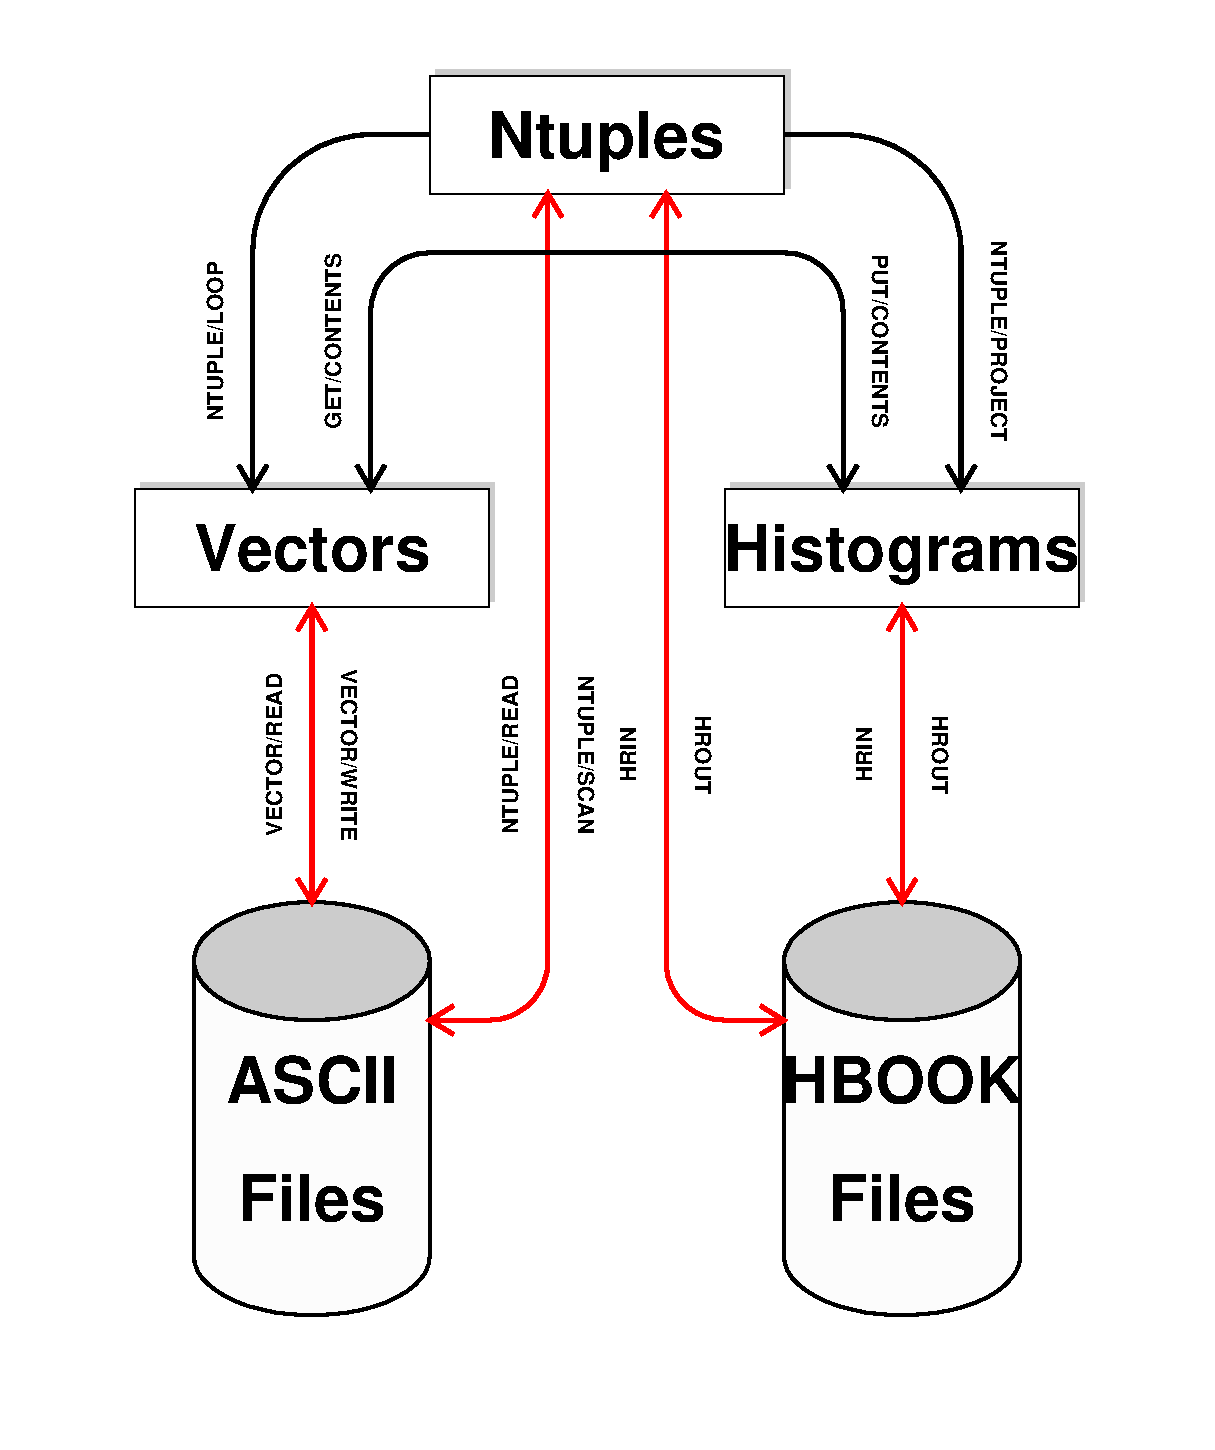
\includegraphics[width=.7\linewidth]{pawtut10.eps}
\caption{PAW entities and their related commands}
\label{fig:PAWCOM}
\end{figure}

Relations which exist between various PAW entities as described in section 
\ref{sec:pawstructure} on page~\pageref{sec:pawstructure}
and the operations which can be performed upon them have been
schematically represented in figure \ref{fig:PAWCOM}.
All commands shown in the picture next to the lines connecting the objects
have been abbreviated in a way that
they are unambiguous and can be typed to PAW, which will then
detail the various parameters to be supplied.
 
There are three main input/output formats, namely a simple text
file (e.g. with data points or commands), a direct access ZEBRA RZ file
(used by HBOOK and HIGZ for storing histograms and pictures on a given
machine) and a ZEBRA FZ sequential file, which can be used to transfer
structured ZEBRA data between various computers.
The RZ and FZ representations can be transformed into each other
using the TOALFA and FRALFA commands.
\index{ZEBRA!TOALFA}
\index{ZEBRA!FRALFA}
\index{ZEBRA!RZ file}
\index{ZEBRA!FZ file}
\index{text!data}
 
The three main PAW objects, Ntuples, histograms and vectors, can be
{\bf printed} on an alphanumeric screen (\Ucom{PRINT}
commands) or they can be plotted on a graphics screen (\Ucom{PLOT}
commands). 
The picture can be transformed into a ZEBRA data structure
and stored in a HIGZ database for later reference (e.g. editing by the
HIGZ editor), or an external presentation can be obtained via the
\index{metafile}
creation of a {\bf metafile}. 
\index{PAW!object}
\index{PRINT!commands}
\index{PLOT!commands}
\index{HIGZ}
\index{metafile}
\index{PostScript}
\index{PAW!entities}

\endinput

%%%%%%%%%%%%%%%%%%%%%%%%%%%%%%%%%%%%%%%%%%%%%%%%%%%%%%%%%%%%%%%%%%%%%%%%%%%%%%%%%
%                                                                              %
%   PAW   - Reference Manual -- LaTeX Source                                   %
%                                                                              %
%   Chapter 3 : PAW Examples                                                   %
%                                                                              %
%   EPS file      : pawtut60b.eps                                              %
%                   example.eps                                                %
%                                                                              %
%   Editor: Michel Goossens / IT-ASD                                           %
%   Last Mod.: 30 July 1998 Olivier Couet                                      %
%                                                                              %
%%%%%%%%%%%%%%%%%%%%%%%%%%%%%%%%%%%%%%%%%%%%%%%%%%%%%%%%%%%%%%%%%%%%%%%%%%%%%%%%
\chapter{PAW by Examples}
\minitoc
\newpage
\section{Basic Principles}
\begin{itemize}
\item \PAW\ (Physics Analysis Workstation) is an {\em interactive system}
       designed for data analysis and data presentation.
\item \PAW\ provides a set of {\em commands} acting on specific objects. The
      main objects or data type are: {\em vectors}, {\em histograms}, and 
      {\em ntuples}. The aim of the examples is to explain how to work with 
      these objects.
\item The \PAW\ commands are organized in a {\em tree}, whose
      general structure is: \texttt{OBJECT/ACTION}. \\
Examples: \Ucom{NTUPLE/PLOT}, \Ucom{HISTOGRAM/PROJECT}, \Ucom{VECTOR/DRAW}
\item The usual user interface is a ``command line interface'': commands are
      typed on keyboard and executed after {\tt <CR>}. Commands parameters
      are separated with blank.
\item Command editing and retrieving is also possible. It is controlled
      via the command {\tt RECALL\_STYLE}.
\item Commands can be grouped into ``Macros''. Macros are files with the
      extension {\tt .kumac} containing \PAW\ commands and flow control
      operators like ``do loop'', ``if endif'', etc .. . To execute
      a macro it is enough to type {\tt EXEC macroname}.
\item online help can be obtained with the commands:
\begin{itemize}
   \item {\tt HELP} to have the full description of a command.
   \item {\tt USAGE} to have only the command syntax.
\end{itemize}
\item A printable version of the reference manual can be obtained with the
      command {\tt MANUAL}.
\item \PAW++ provides a Motif based User Interface to \PAW.
\item \PAW\ and \PAW++ have the SAME basic functionality.
\end{itemize}
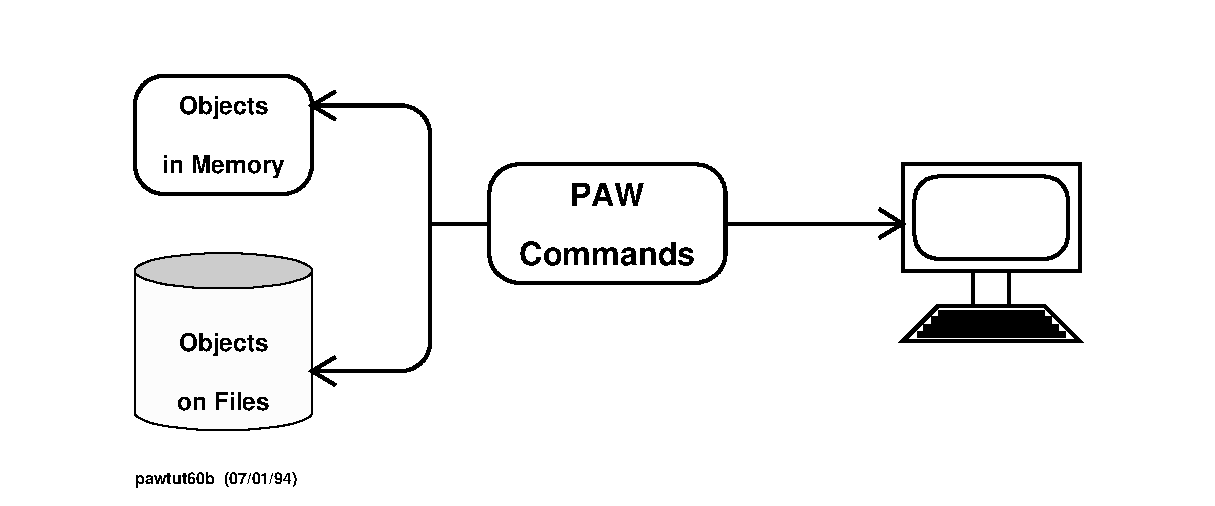
\epsfig{file=pawtut60b.eps,width=\linewidth}
\clearpage

\section{Starting the PAW Tutorial}
This tutorial present the basic principles of \PAW\ using a set of examples
(\PAW\ macros). It tries to cover the most frequently used basic functions of
\PAW.  
In the examples, highlighted points are written in UPPERCASE with a reference
in the left margin. This reference point to a comment after the listing
of the macro. If the example produce a graphics output, it is given on
the page behind the example. Under each figure, the name of the 
corresponding macro is given.

\begin{alltt}
      MACRO PAWLOGON
      Mess '*************************************************************'
      Mess '*                                                           *'
      Mess '*                  Starting PAW examples                    *'
      Mess '*                                                           *'
      Mess '*                     29-30 June 1993                       *'
      Mess '*                                                           *'
      Mess '*************************************************************'
\end{alltt}

This example shows what could be the {\tt MACRO PAWLOGON} (in the file
{\tt PAWLOGON.KUMAC}) which is automatically executed (if it exists) at the
beginning of each \PAW\ session.

It is assumed that the macro {\tt ALDDEF} is executed before each example.

\index{alldef.kumac}
\subsection*{alldef.kumac}
\begin{alltt}
      MACRO ALLDEF
      Size 18 24
      Next
      Set * ; Option * ; Igset *
      Size 18 24
      Histogram/Delete * ; Vector/Delete *
      Title_global ' '
      Title_global ' ' U
      Option NBOX
      Option NGRI
      Set *WID 1
      Set CSIZ 0.25 ; Set VSIZ 0.25 ; Set TSIZ 0.32
      Set XMGL 1.2  ; Set XMGR 1.2  ; Set YMGU 0.5 ; Set YMGL 1.5
      Set GSIZ 0.1
      Set YHTI 0.7
      Set KSIZ 0.15
      Set MTYP 1
      Zone 1 1
      Next
      Return
\end{alltt} 

%%%%%%%%%%%%%%%%%%%%%%%%%%%%%%%%%%%%%%%%%%%%%%%%%%%%%%%%%%%%%%%%%%%%%%%%%%%%%%%%
\clearpage
\section{Vectors---Tutorial}
\label{sec:tutvectors}
\pawtutfig{20}
\clearpage
\pawtutfig{21}
\clearpage
\pawtutfig{28}
\clearpage
\pawtutfig{29}
\clearpage
\section{Vectors---Examples}
\subsection{Starting with vectors}
\begin{alltt}
\Bn{6}     * Starting with vectors
\Bn{6}     VECTOR/CREATE VECT1(10)  | Create a vector of length 10
\Bn{1}     VECTOR/INPUT VECT1 10 8 6 4 2 3 5 7 9 11
\Bnii{7}{1}   VECTOR/CRE VX(20) R 1. 2. 3. 4. 5. 6. 7. 8. 9. _
      10. 11. 12. 13. 14. 15. 16. 17. 18. 19. 20.
      v/cr vy(20) r 1.1 3.2 5.3 7.4 7.5 6.6 4.3 2.1 6.6 _
      11.1 16.2 18.3 19.0 17.8 16.0 12.1 9.1 6.1 3.1 6.6
\Bn{8}     ZON 1 2
\Bn{2}     VECTOR/DRAW VECT1
\Bnii{4}{2}   GRAPH 20 VX VY
\Bnii{4}{5}   graph 20 VX VY *
\Bn{5}     gra 20 VX VY C
\Bn{3}     VECT/DEL *
\end{alltt} 
\begin{DinglistE}
\item Here we see two ways to fill a vector:
\begin{enumerate}
   \item {\tt V/CREATE}: create a vector and, optionally, fill it.
         \index{vector!create}
   \item {\tt V/INPUT}: allows to fill an existing vector.
         \index{vector!input}
\end{enumerate}
We will see other ways later.
\item Graphic representations of vectors : {\tt VECTOR/DRAW} and
      {\tt GRAPH}. \index{vector!draw} \index{vector!graph}
\item {\tt VECT/DELETE} allows to delete a vector from memory. ``*'' means
      delete all vectors in memory. Very often in \PAW\ a command acting
      on a specific kind of objects (vectors, histogram, pictures) can
      access the complete object set with ``*''. \index{vector!delete}

\underline{Note also:}

\item The \PAW\ commands are case insensitive.
\item Command abbreviations are permitted.
\item The character ``*'' and ``$\mid$'' are used for comments.
\item The character ``\_'' is used to indicate a continuation line.
\item The command {\tt ZONE} subdivides the graphical area.
\end{DinglistE}
\pawexfig{1}

%%%%%%%%%%%%%%%%%%%%%%%%%%%%%%%%%%%%%%%%%%%%%%%%%%%%%%%%%%%%%%%%%%%%%%%%%%%%%%%%
\clearpage

\subsection{Some more vector commands}
\begin{alltt}
      vector/create VECT(10,3) R _
      1. 2. 3. 4. 5. 6. 7. 8. 9. 10. _
      9.1 8.1 7.1 6.1 5.1 4.1 3.1 2.1 1.1 0.1 _
      6.2 4.2 3.2 2.2 1.2 1.2 2.2 3.2 4.2 5.2
      vector/create VECT1(10) R _
      1.1 2.2 3.3 4.4 5.5 6.6 5.5 4.4 3.3 2.2
\Bn{5}     SET HTYP 244 ; VE/DR VECT(1:10,3)
\Bnii{1}{2}   VECTOR/DRAW VECT(1:10,3) ! SC
\Bnii{4}{6}   VECTOR/DRAW VECT1 ! L*S
      ve/list
\Bn{3}     VE/WRITE VECT 'vector.data' '(3(10f5.0,/))'
\end{alltt} 
\begin{DinglistE}
\index{vector!draw}
\index{vector!dimensions}
\item A vector can have up to three dimensions. Dimensions which are not
      specified are taken as 1, for example {\tt VEC(10) $\rightarrow$
      VEC(10,1,1)} and {\tt VEC $\rightarrow$ VEC(1,1,1)}.
      \index{vector!subranges}
\item It is possible to access a subrange of a vector, for example:
      {\tt V(2:3)}, {\tt V(3:)} or {\tt V(:5)}. \index{vector!write}
\item The command {\tt VECT/WRITE} creates the file {\tt vector.data}
      as follows:
\begin{verbatim}
     1.   2.   3.   4.   5.   6.   7.   8.   9.  10.
     9.   8.   7.   6.   5.   4.   3.   2.   1.   0.
     6.   4.   3.   2.   1.   1.   2.   3.   4.   5.
\end{verbatim}

\underline{Note also:}

\item The character ``!'' means default value of a parameter.
\item It is possible to have several commands, separated with ``;'', on
      the same line.
\item Many commands have a parameter which defines
      options. Such parameters (often called {\tt CHOPT} or {\tt OPTION})
      have the attribute ``Option'' (see the help). Each option is 
      a character string. It is possible to mix several options, e.g.
      ``{\tt SC}'' or ``{\tt L*S}''.
\end{DinglistE}

\pawexfig{2}

%%%%%%%%%%%%%%%%%%%%%%%%%%%%%%%%%%%%%%%%%%%%%%%%%%%%%%%%%%%%%%%%%%%%%%%%%%%%%%%%
\clearpage

\subsection{Possible data representations with VECTOR/DRAW}
\begin{alltt}
      zone 2 3
      ve/create v(10) R 5 1 3 2 4 1 3 1 8 6
\Bn{1}     SET HTYP 244
      ve/draw v
      ve/draw v ! b
      ve/draw v ! l
\Bn{3}     VE/DRAW V CHOPT=L*
      ve/draw v ! bl*
\Bn{2}     IGSET MTYP 21
      ve/draw v ! e
      ve/de V
\Bn{4}     RETURN
\end{alltt} 
\begin{DinglistE}
\index{vector!draw}
\item The command {\tt SET} defines some high level
      graphics attributes for commands like {\tt VECT/DRAW} or {\tt HIST/PLOT}.
      Here the {\tt HTYP} (Histogram hatch TYPe) is defined.
      \index{IGSET} \index{SET}
\item {\tt IGSET} is used to define basic graphics
      attributes like line width, marker type etc ... . Here the marker
      type is defined. It is possible to type always {\tt SET} instead 
      of {\tt IGSET} i.e. if a {\tt IGSET} parameter is invoke with the
      {\tt SET} command, the command {\tt IGSET} is automatically invoked.
      \index{command!parameter}
\item By default the parameters of a command are positional but it is
      possible to assign values by name, i.e. {\tt PARAMETER=value}. For
      example we have here {\tt CHOPT=L*}. In this case the ``!'' can be
      suppressed.

\underline{Note also:}

\item The statement {\tt RETURN} is not mandatory in a macro except if there
      are several macros in the same file. In this case, a macro within a
      file can be executed by: {\tt EXEC FILENAME\#MACRONAME}.
      \index{\texttt{RETURN}}
\end{DinglistE}
\pawexfig{3}

%%%%%%%%%%%%%%%%%%%%%%%%%%%%%%%%%%%%%%%%%%%%%%%%%%%%%%%%%%%%%%%%%%%%%%%%%%%%%%%%
\clearpage

\subsection{Vectors and Histograms}
\label{sec:vectordrawplot}
\subsection*{Functionality of VECT/DRAW, VECT/PLOT, VECT/HFILL and
  PUT/CONT}
\begin{alltt}
      zone 2 2
      ve/create VECT1(10) R 1 2 3 4 5 5 4 3 2 1
      *
      ve/draw VECT1
\Bn{1}     VE/PLOT VECT1
      *
\Bn{4}     CREATE/1DHISTO 100 'test vector/hfill' 5 1. 6.
      max 100 2.5
\Bn{2}     VE/HFILL VECT1 100
      histo/plot 100 b
      hi/de 100
      *
      create/1dhisto 100 'test put/contents' 10 1. 11.
\Bn{5}     MAX 100 5.5
\Bn{5}     MIN 100 0.5
\Bn{3}     PUT/CONTENTS 100 VECT1
      histo/plot 100
\end{alltt} 
\index{vector!draw}
\index{vector!plot}
\index{vector!hfill}
\index{put!contents}
\begin{DinglistE}
\item {\tt VECT/PLOT} draws the statistic of the given vector.
\item {\tt VECT/HFILL} fills an existing histogram (create with
      {\tt 1DHIST}) with the values taken from a vector. Note that the
      command {\tt VECTOR/PLOT} can automatically book an histogram
      and fill it with the vector content.
\item {\tt PUT/CONT} replaces the content of an histogram with
     the values of a vector.

\underline{Note also:}

\item Histograms are \HBOOK\ objects. They can be created, like here,
      interactively in \PAW\ or in a batch \HBOOK\ program.They can be 
      stored in direct access files (we will see examples later).
\index{histogram!minimum}
\index{histogram!maximum}
\item {\tt MIN} and {\tt MAX} define the minimum and maximum of
      an histogram. By default they are computed automatically.
\end{DinglistE}
\pawexfig{4}

%%%%%%%%%%%%%%%%%%%%%%%%%%%%%%%%%%%%%%%%%%%%%%%%%%%%%%%%%%%%%%%%%%%%%%%%%%%%%%%%
\clearpage

\subsection{Vector operations}
\index{vector!operations}
\begin{alltt}
      zone 1 2
      ve/create V1(10) R 1 2 3 4 5 5 4 3 2 1
      vector/operations/vscale V1 0.5   V12
\Bn{1}     VE/OP/VSCALE             V1 0.25  V14
      ve/dr V1
      ve/dr V12 ! S
      ve/dr V14 ! S
\Bn{1}     VSUB                      V1 V14 V14M
      ve/dr V1
      set htyp 344
      ve/dr V14M ! S
      set htyp 144
      ve/dr V12  ! S
\end{alltt} 
\begin{DinglistE}
\item Some simple operations are possible on vectors:
\begin{verbatim}
      VBIAS     : Y(i) = a + X(i)
      VSCALE    : Y(i) = a * X(i)
      VADD      : Z(i) = X(i) + Y(i)
      VMULTIPLY : Z(i) = Z(i) * Y(i)
      VSUBSTRACT: Z(i) = X(i) - Y(i)
      VDIVIDE   : Z(i) = X(i) / Y(i)
\end{verbatim}
  In these operations the resulting vectors are created automatically.
  Note that for more complicate operations like {\tt SQRT} or trigonometric
  functions etc... , \SIGMA\ must be used (we will see examples later).
\end{DinglistE}
\pawexfig{5}

%%%%%%%%%%%%%%%%%%%%%%%%%%%%%%%%%%%%%%%%%%%%%%%%%%%%%%%%%%%%%%%%%%%%%%%%%%%%%%%%
\clearpage

\subsection{Simple macro, with a loop and a VECTOR fit}

\begin{alltt}
      ve/create VECT(10,3)
\Bn{1}     VE/READ VECT 'vector.data'
      *
      ve/print VECT(1:10,3)
      vbias vect(1:10,1) 0.5 vect(1:10,1)
      zon 1 2
      *
\Bn{4}     DO IP = 2,3
        ve/draw vect(1:10,[ip])
\Bnii{2}{3}     ORDER = [IP] - 1
\Bn{5}       VECT/FIT VECT(1:10,1) VECT(1:10,[IP]) ! P[order] WS
\Bn{4}     ENDDO
      ve/delete VECT
\end{alltt} 
\begin{DinglistE}
\item The file {\tt vector.data} previously created is read again in
      this example via the command {\tt VECT/READ}. Note that it
      is not necessary to specify the format. \index{vector!read}
\item This example shows the usage of variables in the macros ({\tt IP}).
      The content of a variable can be accessed via:
\index{macro!variable}
\index{macro!loop}
\begin{verbatim}
                      [variable]
\end{verbatim}
      Note that the name of a variable in not case sensitive.
\item Simple computations on variables are possible, like {\tt i=[i]+1}
      or {\tt a=[b]+2}. However it is not possible to do complex operations
      on variables. For this kind of computation vectors and \SIGMA\
      (or \COMIS) must be used.
\item Some controls statements are available in macros (see the complete
      list in the next example).
\item It is possible to fit the vectors with functions. Here the
      function used for the fit is a polynome. The fitting mechanisms are very
      complete in \PAW\ and simple to use. All the details useful to use the
      commands {\tt HIST/FIT} and {\tt VECT/FIT} are given in the \PAW\ manual.
\end{DinglistE}
\pawexfig{6}

%%%%%%%%%%%%%%%%%%%%%%%%%%%%%%%%%%%%%%%%%%%%%%%%%%%%%%%%%%%%%%%%%%%%%%%%%%%%%%%%
\clearpage

\subsection{Macros flow control}

There are several constructs available for controlling the flow execution,
which include conditional statement blocks, several looping constructs and
variable assignation.

\index{macro!flow control}
\begin{center}
\begin{tabular}{|l|l|} \hline
\multicolumn{2}{|c|}{\bf Macro Statements} \\ \hline
{\sc Statement}                         & {\sc Description} \\
\hline
{\tt MACRO mname par1=val1 ...}         & begin macro {\tt mname} \\
{\tt EXEC mname par1 par2=val2 ...}     & execute macro {\tt mname} \\
{\tt RETURN}                            & end of a macro \\
{\tt READ par}                 & read macro parameter {\tt par} from keyboard \\
{\tt SHIFT}                             & control parameters list \\
{\tt label:}                            & label (must terminate with a colon) \\
{\tt GOTO label}                        & jump to {\tt label} \\
{\tt ON ERROR GOTO label}  & resume at {\tt label} on error condition \\
{\tt OF ERROR}    & temporarily deactivate the {\tt ON ERROR GOTO} handling   \\
{\tt ON ERROR}    & reactivate the latest {\tt ON ERROR GOTO} handling        \\
{\tt IF logical\_expression GOTO label} & conditional statement \\
{\tt IF-THEN, ELSEIF, ELSE, ENDIF}      & Macro flow control    \\
{\tt CASE, ENDCASE}                     & Macro flow control    \\
{\tt WHILE-DO, ENDWHILE}                & Macro flow control    \\
{\tt REPEAT, UNTIL}                     & Macro flow control    \\
{\tt DO, ENDDO}                         & Macro flow control    \\
{\tt FOR, ENDFOR}                       & Macro flow control    \\
{\tt BREAKL}                            & Macro flow control    \\
{\tt EXITM}                             & Macro termination     \\
par = arithmetic\_expression            & assignment statement  \\
\hline
\end{tabular}
\end{center}

\index{macro!conditional statement}
\subsection*{Conditional statement}
\begin{alltt}
 MACRO DOC1                                        PAW > EXEC DOC1
   A = 10                                          Sum of 10 and 1.5 is 11.5
   NN = 1.5                                        KUIP arithmetic is correct.
   TOT = [A]+[NN]
   IF [TOT] > 11 THEN
     MESSAGE Sum of [A] and [NN] is [TOT]
     AOK = correct
   ELSE
     AOK = wrong
   ENDIF
   MESSAGE KUIP arithmetic is [AOK].
 RETURN
\end{alltt}

\clearpage
\subsection*{Unassigned variables cannot be substituted by their
  values.}
\begin{alltt}
 MACRO DOC2                                        PAW > EXEC DOC2
    A = 10                                         Result of sum is 10+[XX]
    NN = 1.5
    TOT = [A]+[XX]
    MESSAGE Result of sum is [TOT]
 RETURN
\end{alltt}

%%%%%%%%%%%%%%%%%%%%%%%%%%%%%%%%%%%%%%%%%%%%%%%%%%%%%%%%%%%%%%%%%%%%%%%%%%%%%%%%
\clearpage

\subsection{More on fits}
\subsection*{Fit the sine function sin between 0 and $2\pi$}
\begin{alltt}
\Bn{4}     APPLICATION SIGMA
\Bn{4}        alpha=array(100,0#2*PI)
\Bn{4}        sina=sin(alpha)+rndm(alpha)*0.1
\Bn{4}        err=array(100,0.1#0.1)
\Bn{4}     EXIT
      zone 2 2
\Bn{1}     V/FIT ALPHA(1:50) SINA(1:50) ERR(1:50) G
\Bn{1}     V/FIT ALPHA SINA ERR P3
\Bn{1}     V/FIT ALPHA SINA ERR P5
      v/create par(1) r 10.
\Bn{2}     V/FIT ALPHA SINA ERR SINFIT.F ! 1 PAR
\Bn{3}     V/PRI PAR
\end{alltt} 
\begin{DinglistE}
\item In this macro two different types of predefined fits are used: Gaussian,
      Polynomial. As we will see later, the histograms fitting command
      {\tt HISTO/FIT} has exactly the same syntax except that the 3 vectors
      are replaced by an unique parameter: The histogram identifier.
      On histograms some other minimization mechanisms are available via
      the commands {\tt SPLINE}, {\tt SMOOTH}, etc.. .
      \index{vector!fit}
\item It is also possible to defined specific functions. Here the function
      {\tt SINFIT} is defined as follow:
\subsection*{The function {\tt SINFIT}}
\begin{alltt}
      function sinfit(x)
      common /pawpar/ par(1)
      sinfit=par(1)*sin(x)
      end
\end{alltt} 
\item This {\tt VECT/PRI} shows that now {\tt PAR(1)} is close to 1.
\begin{verbatim}
      PAR(1) = 0.994221
\end{verbatim}
\item Vector initialization with \SIGMA. We will see other \SIGMA\ examples
      later.
\end{DinglistE}
\pawexfig{6c}
\clearpage
\subsection*{Output of the Gaussian fit}
\begin{alltt}
     **********************************************
     *                                            *
     * Function minimization by SUBROUTINE HFITV  *
     * Variable-metric method                     *
     * ID =          0  CHOPT =                   *
     *                                            *
     **********************************************
 Convergence when estimated distance to minimum (EDM) .LT.   .10E-03

 FCN=   2221.676     FROM MIGRAD    STATUS=CONVERGED    239 CALLS      240 TOTAL

                     EDM=   .85E-05    STRATEGY= 1      ERROR MATRIX ACCURATE

  EXT PARAMETER                                   STEP         FIRST
  NO.   NAME        VALUE          ERROR          SIZE      DERIVATIVE
   1      P1        1.1316        .24808E-01    .64412E-03    .15289
   2      P2        1.5419        .21417E-01    .62018E-03    .42301E-01
   3      P3       -.76813        .17032E-01    .43531E-03   -.25527
\end{alltt}
\subsection*{Output of the Polynomial fit (P3)}
\begin{alltt}
 CHISQUARE =  .2290E+02  NPFIT =  100
     **********************************************
     *                                            *
     * Function minimization by SUBROUTINE HFITV  *
     * Variable-metric method                     *
     * ID =          0  CHOPT =                   *
     *                                            *
     **********************************************
 Convergence when estimated distance to minimum (EDM) .LT.   .10E-03

 FCN=   49.31862     FROM MIGRAD    STATUS=FAILED        90 CALLS       91 TOTAL
                     EDM=   .79E-01  STRATEGY=1  ERROR MATRIX UNCERTAINTY= 70.2%

  EXT PARAMETER                APPROXIMATE        STEP         FIRST
  NO.   NAME        VALUE          ERROR          SIZE      DERIVATIVE
   1      P1       -.13523        .34965E-02    .00000E+00    5.6896
   2      P2        1.8729        .53793E-02    .00000E+00   -6.8643
   3      P3       -.86391        .32623E-03    .00000E+00    94.054
   4      P4        .91424E-01    .23105E-03    .00000E+00    6.6564

 CHISQUARE =  .5137E+00  NPFIT =  100
\end{alltt}
\clearpage
\subsection*{Output of the Polynomial fit (P5)}
\begin{alltt}
     **********************************************
     *                                            *
     * Function minimization by SUBROUTINE HFITV  *
     * Variable-metric method                     *
     * ID =          0  CHOPT =                   *
     *                                            *
     **********************************************
 Convergence when estimated distance to minimum (EDM) .LT.   .10E-03

 FCN=   7.164283     FROM MIGRAD    STATUS=FAILED       240 CALLS      241 TOTAL
                     EDM=   .19E+01    STRATEGY= 1      ERR MATRIX NOT POS-DEF

  EXT PARAMETER                APPROXIMATE        STEP         FIRST
  NO.   NAME        VALUE          ERROR          SIZE      DERIVATIVE
   1      P1        .46785E-01    .20704E-03    .68172E-07    32.993
   2      P2        .93224        .10038E-02    .74579E-06   -551.05
   3      P3        .20962        .33827E-03    .16770E-06   -3073.1
   4      P4       -.36899        .32674E-03    .29519E-06   -1084.4
   5      P5        .82836E-01    .19712E-04    .66269E-07    821.80
   6      P6       -.52834E-02    .12561E-05    .42267E-08   -5204.8

 CHISQUARE =  .7622E-01  NPFIT =  100
\end{alltt}
\subsection*{Output of the ``\COMIS'' fit}
\begin{alltt}
     **********************************************
     *                                            *
     * Function minimization by SUBROUTINE HFITV  *
     * Variable-metric method                     *
     * ID =          0  CHOPT =                   *
     *                                            *
     **********************************************
 Convergence when estimated distance to minimum (EDM) .LT.   .10E-03

 FCN=   32.13273     FROM MIGRAD    STATUS=CONVERGED     21 CALLS       22 TOTAL
                     EDM=   .92E-05    STRATEGY= 1      ERROR MATRIX ACCURATE

  EXT PARAMETER                                   STEP         FIRST
  NO.   NAME        VALUE          ERROR          SIZE      DERIVATIVE
   1      P1        .99811        .13752E-01    .51510E-04   -.31172

 CHISQUARE =  .3246E+00  NPFIT =  100
\end{alltt}

%%%%%%%%%%%%%%%%%%%%%%%%%%%%%%%%%%%%%%%%%%%%%%%%%%%%%%%%%%%%%%%%%%%%%%%%%%%%%%%%
\clearpage

\subsection{VECTOR/READ using MATCH}
\index{vector!read!using match}
\index{match}
\begin{alltt}
\Bn{1}     V/READ X,Y,Z match.dat 6x,3(F4.1) ! /Data/
      v/draw X
      v/draw Y ! S
      v/draw Z ! S
\end{alltt} 
\subsection*{match.dat}
\begin{alltt}
\Bn{2}     Title: File used for tests of the MATCH parameter in V/READ
      Data : 1.0 2.0 3.0
      Data : 2.0 3.0 4.0
      Data : 3.0 4.0 5.0
      Data : 4.0 5.0 6.0
\Bn{2}     This line will be ignored by a V/READ with MATCH
      Data : 5.0 6.0 7.0
      Data : 6.0 7.0 8.0
      Data : 7.0 8.0 9.0
      Data : 8.0 9.0 1.0
      Data : 9.0 1.0 2.0
\Bn{2}     End
\end{alltt} 
This example shows how the {\tt MATCH} parameter can be used in order to
read only a subset of a file. {\tt MATCH} is used to specify a pattern 
string, restricting the vector filling only to the records in the file 
which verify the pattern. Example of patterns: 
\begin{itemize}
\item     /string/      match a string (starting in column 1)
\item    -/string/      do not match a string (starting in column 1)
\item     /string/(n)   match a string, starting in column n
\item     /string/(*)   match a string, starting at any column
\end{itemize}
\begin{DinglistE}
\item When the {\tt MATCH} parameter is used, the command {\tt V/READ} reads
      the file in two passes:
\begin{enumerate}
\item to find how many lines should be read in order to create vectors with
      the proper length.
\item to read the lines where the {\tt MATCH} parameter is found.
\end{enumerate}
\item these lines are skipped during the reading pass.
\end{DinglistE}
\pawexfig{6d}

%%%%%%%%%%%%%%%%%%%%%%%%%%%%%%%%%%%%%%%%%%%%%%%%%%%%%%%%%%%%%%%%%%%%%%%%%%%%%%%%
\clearpage

\section{Function drawing---Examples}
\index{function!drawing!one-dimensional}
\subsection{Plot a few one-dimensional functions}
\begin{alltt}
\Bn{3}     OPT GRID
\Bn{1}     FUNC/PLOT X*SIN(X)*EXP(-0.1*X)  -10. 10.
\Bn{2}     SET DMOD 2
      func/plot (sin(x)+cos(x))**5    -10. 10. s
      set dmod 3
      func/plot (sin(x)/(x)-x*cos(x)) -10. 10. s
\end{alltt} 
\begin{DinglistE}
\item {\tt FUN/PLOT} allows to plot 2D functions. The character
      ``{\tt x}'' or ``{\tt X}'' is used as the variable name. The command
      {\tt FUN1} is analog to {\tt FUNC/PLOT}
      but it produces also an histogram with the value of the function.
      The number of steps used to compute the function along the X axis
      can be defined via the command {\tt POINTS}.

\underline{Note also:}

\item {\tt SET DMOD} allows to define the line type for the
      drawing the function. Note that {\tt IGSET LTYP} cannot be
      used is this case because in the command {\tt FUN/PLOT} many
      different lines are drawn (axes, boxes, etc ..). So a specific
      attribute must be used ({\tt DMOD}) for the line type of a function
      or an histogram.
\item {\tt OPTION GRID} allows to have a grid on the subsequent plots.
\end{DinglistE}
\pawexfig{7}

%%%%%%%%%%%%%%%%%%%%%%%%%%%%%%%%%%%%%%%%%%%%%%%%%%%%%%%%%%%%%%%%%%%%%%%%%%%%%%%%
\clearpage

\subsection{Plot a one-dimensional function and loop}
\index{function!drawing!one-dimensional}
\begin{alltt}
\Bnii{1}{2}   MACRO PLOT  1=8
      * The Macro parameter is the number of plots to be drawn.
      * the defaults is 8.
      set dmod 1
\Bn{3}     SET XTIC 0.0001
\Bn{3}     SET YTIC 0.0001
      set xval 100.
      set yval 100.
      opt utit
      fun/plot x*sin(x) -10 10
      fun/plot x*cos(x)*sin(x) -10 10 s
      a=[1]-1
      do i=[a],1,-1
        fun/plot x*sin(x)*[i]/[1] -10 10 s
        fun/plot x*cos(x)*sin(x)*[i]/[1] -10 10 s
      enddo
\end{alltt} 
\begin{DinglistE}
\item In this example we can see that macros can have input parameters.
      These parameters can be positional, and they can be
      accessed in the macro via {\tt [n]}, where {\tt n} is the parameter
      number in the input list, or they can be specified by name and they 
      are accessed like variables. The next example gives more details on
      the input parameters management.
\item If one parameter (positional or not) needs to have a default value,
      the value can be specified on the {\tt MACRO} line. At execution time this
      default value is taken if no value is given. Note that for parameters
      given by name, the default value on the line {\tt MACRO} is mandatory.
\item It is possible to define the geometry of a picture via the {\tt SET}
      parameters described on the figure \ref{fig:HPLSET},. In this example
      the size of the tick marks is set to 0 ({\tt XTIC} and {\tt YTIC}).
      But it is not possible to specify: {\tt SET XTIC 0} as, for the
      {\tt SET} command, 0 means default value.
\end{DinglistE}
\pawexfig{8}

%%%%%%%%%%%%%%%%%%%%%%%%%%%%%%%%%%%%%%%%%%%%%%%%%%%%%%%%%%%%%%%%%%%%%%%%%%%%%%%%
\clearpage

\subsection{More on macro input parameters}

\index{macro!parameter list}
\subsection*{Access to the parameter list}
\begin{alltt}
  MACRO P1                                          PAW > exe p1 23 9
  i = 10                                                  23 squared is 529
\Bn{1} FOR p IN [*] [i] 1 2                                    9 squared is 81
    sq = [p] * [p]                                        10 squared is 100
    message [p] squared is [sq]                           1 squared is 1
  ENDFOR                                                  2 squared is 4
\end{alltt}

\index{macro!indexed positional parameters}
\subsection*{Indexed positional parameters}
\begin{alltt}
  MACRO P2                                          PAW > exe p2 23 9 48
\Bn{2} DO i = 1, [#]                                           parameter 1 is 23
\Bn{3}   message parameter [i] is [%i]                         parameter 2 is 9
  ENDDO                                                   parameter 3 is 48
\end{alltt} 
\begin{DinglistE}
\item The * sign allows to access the list of input parameters.
\item The \# sign allows to access the number of input parameters.
\item \% allows to have indexed positional parameters.
\end{DinglistE}
\clearpage
\mbox{}

%%%%%%%%%%%%%%%%%%%%%%%%%%%%%%%%%%%%%%%%%%%%%%%%%%%%%%%%%%%%%%%%%%%%%%%%%%%%%%%%
\clearpage

\subsection{Plot two-dimensional functions}
\index{function!drawing!two-dimensional}
\begin{alltt}
      zone 2 2
\Bn{1}     FUN2 10 ABS(SIN(X)/X)*(COS(Y)*Y) 40 -6 6 40 -6 6
      contour 10 40 0
      hi/de 10
      fun2 10 x*sin(x)*y*sin(y) 40 -10. 10. 40 -10. 10. C
      h/pl 10 surf4
\end{alltt} 
\begin{DinglistE}
\item The command {\tt FUN2} allows to plot 2D functions and fill an
      histogram. The variables names are {\tt X} and {\tt Y}.
\item It is possible to represent a 2D histogram in several ways :
\begin{enumerate}
     \item As a scatter plot.
     \item With proportional boxes.
     \item With a color table.
     \item As a surface plot.
     \item As a surface with color levels.
     \item As a surface with a contour plot on top.
     \item As a surface with Gouraud shading.
     \item As a lego plot.
     \item As a lego plot with colours or shading.
     \item As a line contour plot.
     \item As a table.
     \item As an arrows plot.
\end{enumerate}
\end{DinglistE}
\pawexfig{9}

%%%%%%%%%%%%%%%%%%%%%%%%%%%%%%%%%%%%%%%%%%%%%%%%%%%%%%%%%%%%%%%%%%%%%%%%%%%%%%%%
\clearpage

\subsection{The Mandelbrot distribution}
\index{Mandelbrot distribution}
\subsection*{Calculate and plot (BOX option) the Mandelbrot
  distribution}
\begin{alltt}
\Bn{1}     FUN2 10 mandel.f [1] -2.4 .8 [1] -1.2 1.2 ' '
\Bn{2}     HI/PL 10 BOX
\end{alltt}
\subsection*{FORTRAN Routine MANDEL}
\begin{alltt}
      real function mandel(xp)
      dimension xp(2)
      data nmax/30/
      x=xp(1)
      y=xp(2)
      xx=0.
      yy=0.
      do n=1,nmax
         tt=xx*xx-yy*yy+x
         yy=2.*xx*yy+y
         xx=tt
         if (4..lt.xx*xx+yy*yy) go to 20
      enddo
   20 mandel=float(n)/float(nmax)
      end
\end{alltt} 
\begin{DinglistE}
\item This example shows one of the usages of \COMIS. In this case,
      the name of the function to be plotted by {\tt FUN2} is replaced by a
      \COMIS\ FORTRAN function.
\item {\tt CHOPT=' '} in the command {\tt FUN2} means to fill only the
      histogram without producing the plot which is by default a surface.
      The plot is produced by the command {\tt HIST/PLOT}.
\item The vector {\tt XP} is an input parameter given by {\tt FUN2}, for
      each cell, to the FORTRAN program. {\tt XP} contains the {\tt X}
      and {\tt Y} coordinates of each cell. You can try to insert:
\begin{verbatim}
      print*, XP
\end{verbatim}
  in {\tt mandel.f} to see the values changing (in this case it is better to
  set the input parameter of the macro to 10).
\end{DinglistE}
\pawexfig{10}

%%%%%%%%%%%%%%%%%%%%%%%%%%%%%%%%%%%%%%%%%%%%%%%%%%%%%%%%%%%%%%%%%%%%%%%%%%%%%%%%
\clearpage

\subsection{Three-dimensional functions drawing}
\index{function!drawing!three-dimensional}
\subsection*{{\tt FUNCTION/DRAW} and {\tt RANGE}}
\begin{alltt}
      zon 2 2
\Bn{1}     FUN/DRAW X**2+Y**2+Z**2=1
\Bn{2}     RANGE 0 1
\Bn{1}     FUN/DRAW X**2+Y**2+Z**2=1
\Bn{2}     RANGE 0 1 0 1
\Bn{1}     FUN/DRAW X**2+Y**2+Z**2=1
\Bn{2}     RANGE 0 1 0 1 0 1
\Bn{1}     FUN/DRAW X**2+Y**2+Z**2=1
\end{alltt} 
\begin{DinglistE}
\item This command draws a sphere of radius 1. The function can
      be also a \COMIS\ program.
\item The command {\tt RANGE} modify the X, Y and Z range
      in which the function is drawn. \index{function!range}
\end{DinglistE}
\pawexfig{10a}

%%%%%%%%%%%%%%%%%%%%%%%%%%%%%%%%%%%%%%%%%%%%%%%%%%%%%%%%%%%%%%%%%%%%%%%%%%%%%%%%
\clearpage
\section{Histograms---Tutorial}
\pawtutfig{30}
\clearpage
\pawtutfig{31}
\clearpage
\pawtutfig{32}
\clearpage
\pawtutfig{33}
\clearpage
\pawtutfig{34}
\clearpage
\pawtutfig{35}
\clearpage
\pawtutfig{36}
\clearpage
\pawtutfig{37}
\clearpage
\pawtutfig{38}
\clearpage
\pawtutfig{39}
\clearpage
\pawtutfig{65}
\clearpage
\pawtutfig{66}
\clearpage

%%%%%%%%%%%%%%%%%%%%%%%%%%%%%%%%%%%%%%%%%%%%%%%%%%%%%%%%%%%%%%%%%%%%%%%%%%%%%%%%
\section{Histograms---Examples}
\subsection{Histograms creation}
\index{histogram!creation}
\subsection*{Creation of one and two dimensional histograms}
\begin{alltt}
      zon 1 2
      function/fun1 100 htfun1.f 100. 0. 1.
      1dh  110 'Test 1-dim Histo' 100 0. 1. 1000.
\Bn{1}     CALL UROUT.F(5000)
\Bn{6}     FUN/FUN2 200 HTFUN2 25. 0. 1. 25. 0. 1. C
      hi/li
\Bnii{3}{5}   HISTOGRAM/FILE 1 PAWHISTS.HBOOK 1024 N
\Bn{4}     HROUT 0
\end{alltt}
\begin{minipage}[t]{8.9cm}
\subsection*{The FORTRAN Routine HTFUN1}
\begin{alltt}
      function htfun1(x)
      data c1,c2,xm1,xm2,xs1,xs2
     +/1.,0.5,0.3,0.7,0.07,0.12/
      a1=-0.5*((x-xm1)/xs1)**2
      a2=-0.5*((x-xm2)/xs2)**2
      x1=c1
      x2=c2
      if(abs(a1).gt.0.0001)x1=c1*exp(a1)
      if(abs(a2).gt.0.0001)x2=c2*exp(a2)
      htfun1=x1+x2
      end
\end{alltt}
\end{minipage}
\begin{minipage}[t]{8.9cm}
\subsection*{The FORTRAN Routine HTFUN2}
\begin{alltt}
\Bn{6}     function htfun2(x,y)
      htfun2=100*htfun1(x)*htfun1(y)
      end
\end{alltt}
\subsection*{The FORTRAN Routine UROUT}
\begin{alltt}
      subroutine urout(nev)
      do i=1,nev
\Bn{2}        x=HRNDM1(100,I)
\Bn{2}        CALL HFILL(110,X,0.,1.)
      enddo
      end
\end{alltt}
\end{minipage}

\begin{DinglistE}
\item In this example \COMIS\ is used  in the simplest way, via the
      command {\tt CALL} ({\tt CALL UROUT.F}). This command just
      calls the FORTRAN routine given as parameter and executes it.
\item It is possible to call several routines of the CERN library. {\tt HELP
      CALL} gives the list of available routines (see next page). Here the
      routines {\tt HRNDM1} and {\tt HFILL} (to fill an histogram) are called
      by {\tt UROUT}. \index{histogram!filling}
\item It is possible to store the histograms in memory into a direct access
      file opened via the command {\tt HIST/FILE}. Here {\tt CHOPT=N} means:
      ``create a New \HBOOK\ file''. If the first parameter ({\tt LUN})
      is 0 the next free logical unit will be used. 
\item To store an histogram in a file it is enough to execute the command
      {\tt HROUT}. {\tt HROUT 0} (or {\tt HROUT *}) stores all the
      histograms currently in memory.
      \index{histogram!file}
\item Several files can be attached via {\tt HIST/FILE} during a \PAW\ session.
      To change the current file it is enough to execute {\tt CD //LUNn} 
      where ``{\tt n}'' is the first parameter given to 
      {\tt HI/FILE}. Note that the command {\tt LD //} gives the
      list of all the files currently attached. Each attached direct access 
      file is similar to a directory (cf UNIX).
\item {\tt HTFUN2} is in the file {\tt htfun1.f}. That is why it can be
      invoked without the extension {\tt .f} because it has been compiled
      during the {\tt CALL} to {\tt htfun1}.
\end{DinglistE}
Most of the time, the histograms are created and filled outside \PAW\
in batch programs calling \HBOOK\ directly, and after interactively
analyzed with \PAW.
\pawexfig{11}
\clearpage
The following routines from the CERN Program Library can be called:
\subsection*{From HBOOK}
\begin{alltt}
      HBOOK1,HBOOK2,HBOOKN,HFILL,HF1,HPRINT,HDELET,HRESET
      HFITGA,HFITPO,HFITEX,HPROJ1,HPROJ2,HFN,HGFIT
      HROPEN,PAOPEN,PACLOS,PAREAD,PAWRIT,HCDIR,HGIVEN
      HTITLE,HBFUN1,HBFUN2,HRNDM1,HRNDM2,HBARX,HBARY
      HPAK,HPAKE,HUNPAK,HGIVE,HGN,HGNF,HGNPAR,HF2,HFF1,HFF2
      HRIN,HROUT,HI,HIE,HIX,HIJ,HIF,HIDALL,HNOENT,HX,HXY
      HTITLE,HCOPY,HSTATI,HBPROF,HOPERA,HIDOPT,HDERIV
      HMAXIM,HMINIM,HMAX,HMIN,HSUM,HNORMA,HREND
      HEXIST,HRGET,HRPUT,HSCR,HFIND,HCX,HCXY,HLABEL
      HBPROX,HBPROY,HBANDX,HBANDY,HBSLIX,HBSLIY
      HBOOKB,HBSTAT,HDIFF,HUNPKE,HREBIN,HERROR
      HOUTPU,HERMES,HISTDO,HFUNC,HIJXY,HXYIJ,HLPOS,HFC1
      HSPLI1,HSPLI2,HMDIR,HLDIR,HLOCAT,HFITH,HFITV,HFINAM
      HBNT,HBNAME,HBNAMC,HFNT,HFNTB,HGNT,HGNTF,HGNTV,HBSET
\end{alltt}
\subsection*{From HPLOT}
\begin{alltt}
      HPLOT,HPLSYM,HPLERR,HPLEGO,HPLNT,HPLSUR,HPLSOF
      HPLABL,HPLSET,HPLGIV,HPLOC,HPLTOC,HPLNEW,HPLOPT
\end{alltt}
\subsection*{From ZEBRA}
\begin{alltt}
      FZIN,FZOUT,FZFILE,FZENDI,FZENDO
      RZCDIR,RZLDIR,RZFILE,RZEND,RZIN,RZOUT,RZVIN,RZVOUT
      RZOPEN,RZIODO
\end{alltt}
\subsection*{From KUIP}
\begin{alltt}
      KUGETV,KUDPAR,KUVECT,KILEXP,KUTIME,KUEXEL,KUPROS
      KUNWG,KUCMD,KUGUID,KUNDPV,KUPAR,KUPVAL,KUACT
\end{alltt}
\clearpage
\subsection*{From HIGZ}
\begin{alltt}
      IPL,IPM,IFA,IGTEXT,IGBOX,IGAXIS,IGPIE,IGRAPH,IGHIST
      IGARC,IGLBL,IGRNG,IGMETA,IGSA,IGSET,IRQLC,IRQST,ISCR
      ISELNT,ISFAIS,ISFASI,ISLN,ISMK,ISVP,ISWN,ITX,ICLRWK
      IGPAVE,IGTERM
\end{alltt}
\subsection*{From KERNLIB}
\begin{alltt}
      VZERO,UCOPY,RNDM,RANNOR,LENOCC,SBIT0,SBIT1,SBYT
      JBIT,JBYT,UCTOH,UHTOC,CLTOU,CUTOL
      ERF,ERFC,FREQ,PROB
\end{alltt}
\subsection*{The following common blocks may be referenced}
\begin{alltt}
     /PAWC/, /QUEST/, /KCWORK/, /PAWPAR/, /PAWIDN/
     /HCFITS/, /HCFITD/
\end{alltt}

%%%%%%%%%%%%%%%%%%%%%%%%%%%%%%%%%%%%%%%%%%%%%%%%%%%%%%%%%%%%%%%%%%%%%%%%%%%%%%%%
\clearpage

\subsection{Read histograms from file and plot}
\begin{alltt}
\Bn{1}     HISTOGRAM/FILE 1 PAWHISTS.HBOOK
\Bn{2}     HRIN  *
\Bn{3}     LDIR
\Bn{3}     HI/LIST
\Bn{5}     ZON 2 2
      hi/pl 100
      set htyp 244
      hi/pl 110
\Bn{5}     ZONE 1 2 2 'S'
      hi/plot 200
\Bn{4}     CLOSE 1
\end{alltt} 
\begin{DinglistE}
\item In this example the existing file {\tt PAWHISTS.HBOOK} is
      attached in {\tt READ-ONLY} mode.
\item The command {\tt HRIN *} (or {\tt HRIN 0}) gets all the
      histograms from the file {\tt PAWHISTS.HBOOK} into the memory. Note
      that commands like {\tt HIST/PLOT} take automatically the histogram
      from the file if it is not already in memory.
      \index{histogram!plot}
      \index{histogram!list}
\item Both {\tt LDIR} and {\tt HI/LIST} give the list of the histograms.
      {\tt LDIR} is the generic command to list the content of a \ZEBRA\
      file. It has no knowledge about the objects stored in the
      file that's why it cannot retrieve the histogram names. 
      The \HBOOK\ specific command {\tt HIST/LIST} is able to find
      informations on the histogram like the histogram title and the
      histogram type.
      On the next page is given the output of these two commands.
\item To release an histogram file it is enough to do {\tt CLOSE n}
      where ``{\tt n}'' is the logical unit number used by the command
      {\tt HIST/FILE} (the first parameter of this command).
      \index{histogram!file}

\underline{Note also:}

\item The usage of the command {\tt ZONE}. It is used two times
      to define zones with different sizes.
\end{DinglistE}
\pawexfig{12}
\clearpage
\begin{center}
\subsection*{Output of LDIR}
\begin{alltt}
 ************** Directory ===> //LUN1 <===

                  Created 911128/1154  Modified 911128/1154


 ===> List of objects
     HBOOK-ID  CYCLE   DATE/TIME   NDATA   OFFSET    REC1    REC2
        100       1   911128/1154    152       1       3
        110       1   911128/1154     85     153       3
        200       1   911128/1154    778     238       3

  Number of records =    2  Number of megawords =  0 +  2039 words
  Per cent of directory quota used =    .050
  Per cent of file used            =    .050
  Blocking factor                  =  49.561
\end{alltt}
      \index{histogram!list}
\subsection*{Output of HIST/LIST}
\begin{alltt}
 ===> Directory :
        100 (1)   htfun1.f
        110 (1)   Test 1-dim Histo
        200 (2)   htfun2
\end{alltt}
\end{center}
\clearpage
\mbox{}

%%%%%%%%%%%%%%%%%%%%%%%%%%%%%%%%%%%%%%%%%%%%%%%%%%%%%%%%%%%%%%%%%%%%%%%%%%%%%%%%
\clearpage

\subsection{Histogram archiving}

\index{histogram!archiving}
In this example, the histograms in an existing \HBOOK\ file are moved
in a new \HBOOK\ file in two separated directories according to their type.

\subsection*{Histogram archiving and directories into \HBOOK\ files}
\begin{alltt}
\Bn{1}     HISTOGRAM/FILE 0 pawtut.hbook
      hi/li
      hrin  *
      close 1
\Bn{2}     HISTOGRAM/FILE 0 pawtutnew.hbook ! N
\Bn{3}     MDIR 1Dhistograms
\Bn{3}     MDIR 2Dhistograms
      ldir
      cd 1Dhistograms
\Bn{4}     HROUT 514,30001,60202
      ldir
      cd //LUN1/2Dhistograms
\Bn{4}     HROUT 8001,1103,11,12
      ldir
      close 1
\end{alltt}{} 
\begin{DinglistE}
\item Attach an existing \HBOOK\ file.
\item Create a new \HBOOK\ file.
\item Create two subdirectories in the file {\tt pawtutnew.hbook}.
      \index{histogram!file!subdirectories}
\item Store the 1d and 2d histograms in two separated directories.
      Some commands like {\tt HROUT} are able to loop
      on parameters if a list is given. Such parameters have the
      attribute ``Loop'' when a help is performed on the command.
\end{DinglistE}
\clearpage
\subsection*{Output of LDIR}
\begin{alltt}
 ===> Directory :
         10 (N)   CERN Population
        514 (1)   Angular density
      30001 (1)   mix
      60202 (1)   p dy like
       8001 (2)   Data (gluino)
       1103 (2)   Charged particle theta vs. phi
         11 (2)   PHI VS. Y  +VE    WEIGHTED
         12 (2)   PHI VS. Y  +VE    WEIGHTED

 ************** Directory ===> //LUN1 <===

                  Created 930602/1428  Modified 930602/1428


 ===> List of subdirectories
 1DHISTOGRAMS     Created 930602/1428 at record     3
 2DHISTOGRAMS     Created 930602/1428 at record     4

 ===> List of objects
     HBOOK-ID  VARIABLE                             CYCLE    DATE/TIME   NDATA

 ************** Directory ===> //LUN1/1DHISTOGRAMS <===

                  Created 930602/1428  Modified 930602/1428


 ===> List of objects
     HBOOK-ID  VARIABLE                             CYCLE    DATE/TIME   NDATA
        514         0                                   1   930602/1428    153
      30001         0                                   1   930602/1428    200
      60202         0                                   1   930602/1428    152

 ************** Directory ===> //LUN1/2DHISTOGRAMS <===

                  Created 930602/1428  Modified 930602/1428


 ===> List of objects
     HBOOK-ID  VARIABLE                             CYCLE    DATE/TIME   NDATA
       8001         0                                   1   930602/1428    537
       1103         0                                   1   930602/1428   5361
         11         0                                   1   930602/1428    444
         12         0                                   1   930602/1428  13114
\end{alltt}

%%%%%%%%%%%%%%%%%%%%%%%%%%%%%%%%%%%%%%%%%%%%%%%%%%%%%%%%%%%%%%%%%%%%%%%%%%%%%%%%
\clearpage

\subsection{Multiple fits on histograms}
\index{histogram!fit}
\subsection*{Fit of the histogram 110 with two Gaussians}
\begin{alltt}
      histogram/File 1 pawhists.hbook
      hrin  *
\Bn{1}     VECT/CREATE PAR(6)
      histo/plot 110
\Bn{5}     SET FWID 6
\Bn{5}     SET DMOD 2
\Bn{2}     HISTO/FIT 110(1:50) G QS 0 PAR(1:3)
\Bn{3}     HISTO/FIT 110(50:100) G QS 0 PAR(4:6)
\Bn{5}     SET DMOD 1
\Bn{4}     HISTO/FIT 110 G+G QS 6 PAR
\end{alltt} 
\begin{DinglistE}
\item The vector {\tt PAR} will be used to get the initial values
      of the fit parameters.
\item Compute a gaussian fit on the first 50 channels. After this command 
      the gaussian parameters are stored in {\tt PAR(1:3)}.
\item Compute a gaussian fit on the last 50 channels. After this command
      the gaussian parameters are stored in {\tt PAR(4:6)}.
\item Compute the global fit using {\tt PAR} for initial values. 

\underline{Note also:}

\item The first two gaussian fits are drawn with dashed lines and the third
      one with a solid line.
\end{DinglistE}
\pawexfig{12b}

%%%%%%%%%%%%%%%%%%%%%%%%%%%%%%%%%%%%%%%%%%%%%%%%%%%%%%%%%%%%%%%%%%%%%%%%%%%%%%%%
\clearpage

\subsection{Histogram operations}
\index{histogram!operations}
\subsection*{Perform operations on histograms read from file and save
  results}
\begin{alltt}
\Bn{1}     HISTOGRAM/FILE 1 PAWHISTS.HBOOK ! U
      hrin  *
      zon 2 2
      opt grid
      igset mtyp 26
      hi/pl 110 e
      hi/pl 110 pl
      zon 1 2 2 s
\Bn{2}     HI/OP/ADD 110 110 120 0.5 0.
      hi/op/add 110 110 130 0.25 0.
      set htyp 245
      hi/pl 110
      set htyp 254
\Bn{3}     HI/PL //PAWC/120 s
      set htyp 253
      hi/pl //PAWC/130 s
      text 0.55 95. 'LEP Very Preliminary' 0.35 25.
      hrout 0
\end{alltt} 
\begin{DinglistE}
\item The option ``{\tt U}'' (for Update) in the command {\tt HIST/FILE}, is
      used when the user wants to change the content of an existing histogram
      file by adding a new histogram ({\tt HROUT} p 166) or deleting an
      histogram ({\tt HSCRATCH} p 166).
\item It is possible to perform operations between histograms like addition
      with the commands in the menu {\tt HISTOGRAM/OPERATIONS}.
\item The memory, like the attached files, can be considered as a directory.
      This is the current directory by default and {\tt //PAWC} is its name.
      The command {\tt HI/PL //PAWC/id} plots the histogram ``{\tt id}'' in
      memory while the current directory is {\tt //LUN1}.
\index{directory!current}
\index{directory!\texttt{PAWC}}
\end{DinglistE}
\pawexfig{13}
\clearpage
\subsection*{How to embellish the graphical ouputs}
\begin{alltt}
      histogram/file 1 pawhists.hbook ! u
      hrin  0
      zon 2 2
      opt grid
\Bn{1}     SET *FON -60
\Bn{2}     SET BWID 4
\Bn{3}     SET BCOL 1.5
      igset mtyp 26
      hi/pl 110 e
      hi/pl 110 pl
      zon 1 2 2 s
      hi/op/add 110 110 120 0.5 0.
      hi/op/add 110 110 130 0.25 0.
      set htyp 245
      hi/pl 110
      set htyp 254
      hi/pl //pawc/120 s
      set htyp 253
      hi/pl //PAWC/130 s
\Bn{4}     IGSET CHHE .35
\Bn{4}     IGSET TANG 25.
\Bn{4}     ITX 0.55 95. 'LEP Very Preliminary'
      hrout 0
\end{alltt} 
\begin{DinglistE}
\item All the text fonts used for {\tt HISTO/PLOT} are set to -60.
\item The line width for the boxes around the histograms is set to 4 pixels.
      Like for the fonts it is possible to do {\tt SET *WID} to set all the
      width available in the {\tt SET} command.
\item The color of the shadow around the histograms is set to 5 (Yellow), it
      appears grey on black and white PostScript printers.
\item To access hardware fonts (ie PostScript fonts) the command {\tt ITX} and
      its related attributes should be used.
\end{DinglistE}
\pawexfig{13b}

%%%%%%%%%%%%%%%%%%%%%%%%%%%%%%%%%%%%%%%%%%%%%%%%%%%%%%%%%%%%%%%%%%%%%%%%%%%%%%%%
\clearpage

\subsection{Keep and update histograms}
\index{histogram!update}
\index{histogram!operations!graphical}
\subsection*{Graphical operations on histograms (Keep and Add)}
\begin{alltt}
      histogram/file 1 pawhists.hbook
      zone 1 2
      set htyp 245
\Bn{1}     H/PL 120 K
      set htyp 254
\Bn{1}     H/PL 110
      set htyp
\Bn{2}     H/PL 110 +
      set htyp 144
      hi/pl 130 +
\end{alltt} 
\begin{DinglistE}
\item The option ``{\tt K}'' in the command {\tt HIST/PLOT} keep the histogram
      in memory at the graphics level to allow updating. If no zone is
      defined, the option ``{\tt K}'' is not necessary.
\item If an histogram is kept in memory (automatically or via option
      ``{\tt K}'') it is possible to add the content of an other histogram
      with option ``+''.
\end{DinglistE}
\pawexfig{24}

%%%%%%%%%%%%%%%%%%%%%%%%%%%%%%%%%%%%%%%%%%%%%%%%%%%%%%%%%%%%%%%%%%%%%%%%%%%%%%%%
\clearpage

\subsection{Playing with dice}
\index{histogram!operations!graphical}
\subsection*{Graphical operations on histograms (Keep and Update)}
\begin{alltt}
      MACRO DICE 1=50
      set hcol 1001
      set ndvx -11.05
\Bn{6}     OPT STAT
\Bn{1}     CALL DICE.F([1])
      hi/fit 3 g
\end{alltt}
\subsection*{FORTRAN routine dice}
\begin{alltt}
      subroutine dice(n)
      ifirst=1
\Bn{2}       CALL HBOOK1(3,'Playing with two dice',11,2.,13.,0.)
        do 3 j=1,n
          ix1=6.*rndm(.01234)+1
          ix2=6.*rndm(.56789)+1
\Bn{3}         CALL HFILL(3,FLOAT(IX1+IX2),0.,1.)
          if (ifirst.eq.1) then
\Bn{4}            CALL HPLOT(3,'BK',' ',0)
             ifirst=0
          else
\Bn{5}            CALL HPLOT(3,'BU',' ',0)
          endif
        enddo
      end
\end{alltt} 
\begin{DinglistE}
\item This macro call a \COMIS\ routine only to be faster. The \COMIS\
      routine can be replaced by a macro, in particular the options
      ``{\tt K}'' and
      ``{\tt U}'' are also available in command {\tt HIST/PLOT}
      (try {\tt HELP H/PL}).
\item The histogram is also booked in the FORTRAN program. The corresponding
      \PAW\ command is {\tt 1DHISTO}.
\item Two random numbers between 1 and 6 are generated and the histogram
      is filled with the sum of this numbers to simulate dice playing.
\item The first time the histogram is plotted the option ``{\tt K}'' is used
      to keep in memory a copy of the histogram in order to update it later.
\item With the ``{\tt U}'' option, \PAW\ looks at the current kept histogram
      contents and update the plot with the new contribution without redrawing
      everything. This mechanism is used in data acquisition.
\item The statistics are also updated.
\end{DinglistE}
\clearpage
\mbox{}


%%%%%%%%%%%%%%%%%%%%%%%%%%%%%%%%%%%%%%%%%%%%%%%%%%%%%%%%%%%%%%%%%%%%%%%%%%%%%%%%
\clearpage

\subsection{Two-dimensional histograms representations}
\index{histogram!two-dimensional representations}
\begin{alltt}
      histogram/file 1 pawhists.hbook
      zon 2 2
\Bn{1}     HI/PL 200 BOX
\Bn{1}     CONTOUR 200 20 0
\Bn{1}     LEGO 200
\Bn{1}     SURFACE 200
      hi/del *
\end{alltt} 
\begin{DinglistE}
\item As we have already seen, the command H/PL allows to draw 2D
      histograms in different ways. Three additional commands are also
      available:
\begin{verbatim}
  * /HISTOGRAM/2D_PLOT/CONTOUR  [ ID NLEVEL CHOPT PARAM ]
  * /HISTOGRAM/2D_PLOT/SURFACE  [ ID THETA PHI CHOPT ]
  * /HISTOGRAM/2D_PLOT/LEGO     [ ID THETA PHI CHOPT ]
\index{histogram!contour}
\index{histogram!surface}
\index{histogram!lego}
\end{verbatim}
      These commands have more parameters than {\tt HIS/PLOT}. For example
      {\tt CONTOUR} allows to specify a set of levels to be drawn
      via the parameter {\tt PARAM} (see next example).
\item Note that it is also possible to have 1D histograms represented as
      lego or surface plots. For example you can do: {\tt HI/PLOT 110 LEGO}.
\end{DinglistE}
\pawexfig{14}

%%%%%%%%%%%%%%%%%%%%%%%%%%%%%%%%%%%%%%%%%%%%%%%%%%%%%%%%%%%%%%%%%%%%%%%%%%%%%%%%
\clearpage

\subsection{Non equidistant contour plots}
\index{histogram!contour!non equidistant}
\subsection*{User defined non equidistant contour plots}
\begin{alltt}
      histogram/file 1 pawhists.hbook
\Bn{1}     VECTOR/CREATE LEVEL(8) R  10 11 12 13 14 15 90 99
      zone 1 2
\Bn{2}     CONTOUR 200 8 2 LEVEL
      arrow .8 .75 .5 .54 .2
\Bn{5}     ARROW .8 .75 .5 .44 .2
\Bn{4}     SET CHHE .28
\Bn{3}     ITX .81 .5 '10.0'
      Arrow .5 .32 .1 .28 .2
      Itx .51 .1 '100.0'
      option LOGY
      h/plot 200 BOX
\Bn{6}     ARROW .5 .32 .1 .28 .2
\Bn{6}     ITX .51 .1 '100.0'
      close 1
\end{alltt} 
The command {\tt CONTOUR} allows to draw user defined levels.
\index{histogram!contour}
\begin{DinglistE}
\item The vector {\tt LEVEL} contains the list of 8 levels to
      be drawn.
\item Only the levels specified in the the vector {\tt LEVEL} are drawn.

\underline{Note also:}

\item Some comments can be drawn with the command {\tt ITX}.
      \index{text}
\item The size of the text is in centimeters even if the position is
      in histogram coordinates (current normalization transformation).
\item The position of the arrow is in the current normalization transformation
      (here histogram coordinates), but its size is in centimeters (last
      parameter. Here 0.2).
\item Arrows and text can be drawn in logarithmic coordinates. For lines
      the logarithm should be computed with \SIGMA.
\end{DinglistE}
\pawexfig{14b}

%%%%%%%%%%%%%%%%%%%%%%%%%%%%%%%%%%%%%%%%%%%%%%%%%%%%%%%%%%%%%%%%%%%%%%%%%%%%%%%%
\clearpage

\subsection{Coordinate systems}
\subsection*{Coordinate systems with legos and surfaces}
\begin{alltt}
      histogram/file 1 pawhists.hbook
      zon 2 2
\Bn{2}     OPT UTIT
\Bn{2}     TITLE 'Polar coordinates' U
\Bn{1}     HI/PL 200 LEGO,POL
      title 'Cylindrical coordinates' U
\Bn{1}     HI/PL 200 LEGO,CYL
      title 'Spherical coordinates' U
\Bn{1}     HI/PL 200 LEGO,SPH
      title 'Pseudo rapidity coordinates' U
\Bn{1}     HI/PL 200 LEGO,PSD
      close 1
\end{alltt}
\index{coordinate systems!polar}
\index{coordinate systems!cylindrical}
\index{coordinate systems!spherical}
\index{coordinate systems!pseudo rapidy}
\begin{DinglistE}
\item Legos and Surfaces plot can be drawn in Polar, Cylindrical,
      Spherical and Pseudo rapidity coordinates. 

\underline{Note also:}

\item The option {\tt UTIT} allows to use ``user title'' on histogram. To
      define the title itself, the command {\tt TITLE} should be
      used with the option {\tt U}. Without this option {\tt TITLE}
      define the global title.
\index{title}
\end{DinglistE}
\pawexfig{14c}

%%%%%%%%%%%%%%%%%%%%%%%%%%%%%%%%%%%%%%%%%%%%%%%%%%%%%%%%%%%%%%%%%%%%%%%%%%%%%%%%
\clearpage

\subsection{Logarithmic scales on lego and surface plots}
\index{logarithmic scale!on lego plots}

\begin{alltt}
      histogram/file 1 pawhists.hbook
      zon 2 2
      opt utit
      hi/pl 200 lego
\Bn{1}     OPT LOGX
      hi/pl 200 lego
\Bn{1}     OPT LOGY
      hi/pl 200 lego
\Bn{1}     OPT LOGZ
      hi/pl 200 lego
      close 1
\end{alltt}
\begin{DinglistE}
\item Logarithmic are possible on Legos and Surfaces plot. It works also
      in Polar, Cylindrical, Spherical and Pseudo rapidity coordinates. 
\end{DinglistE}
\pawexfig{14d}

%%%%%%%%%%%%%%%%%%%%%%%%%%%%%%%%%%%%%%%%%%%%%%%%%%%%%%%%%%%%%%%%%%%%%%%%%%%%%%%%
\clearpage

\subsection{Subranges in histogram identifiers}
\index{histogram!subrange}

\begin{alltt}
      histogram/file 1 pawhists.hbook
      hrin  0
      close 1
\Bn{4}     TRACE ON
      zon 2 2
\Bn{1}     HI/PL 110(56:95) E
\Bn{4}     * Comments are not printed in TRACE mode
      hi/pl 200(8:8,)      box
\Bn{3}     HI/PL 200(3:15,3:15) CONT
\Bn{4}     TRACE OFF
\Bn{2}     hi/pl 200(0.:12,0.1:0.5) LEGO
\end{alltt} 
\begin{DinglistE}
\item This example shows how to plot subranges of 1D or 2D histograms.
      The different possibility to give the range are the following:
\begin{enumerate}
\item  {\tt id(n1:n2)} with {\tt n1 $\geq$ n2}.
\item  {\tt id(n1:)} in this case {\tt n2 = number of bins}.
\item  {\tt id(:n2)} in this case {\tt n1 = 1}.
\end{enumerate}
\item If {\tt n1} or {\tt n2} are integer they are consider as bin
      numbers. But if they are real they are consider axis values.
      Note that bin values and axis values can be mixed inside the
      same range definition.
\item In case of 2D histograms, the two ranges are separate with ``,''.

\underline{Note also:}

\item The {\tt TRACE} command sets {\tt ON} or {\tt OFF} the trace mode.
      When this mode is on, all the command executed inside macros are
      displayed on the standard output.
\begin{center}
\subsection*{Ouput of the TRACE mode}
\begin{alltt}
 >>>>> zon 2 2
 >>>>> HI/PL 110(56:95) E
 >>>>> hi/pl 200(8:8,)      box
 >>>>> HI/PL 200(3:15,3:15) CONT
 >>>>> TRACE OFF
\end{alltt}
\end{center}
\end{DinglistE}
\pawexfig{15}

%%%%%%%%%%%%%%%%%%%%%%%%%%%%%%%%%%%%%%%%%%%%%%%%%%%%%%%%%%%%%%%%%%%%%%%%%%%%%%%%
\clearpage

\subsection{Stacked Lego plots and subranges}
\index{histogram!stacked lego plots}
\index{histogram!subrange}
\begin{alltt}
      hi/file 1 pawhists.hbook
      zon 2 2
\Bn{1}     HIST/PLOT 200(0.:0.5,0.:0.5) LEGO1
\Bn{1}     HIST/PLOT 200(0.5:1.,0.5:1.) LEGO1
      zon 1 2 2 s
\Bn{3}     OPTION BAR
\Bn{2}     HIST/PLOT 200(0.:0.5,0.:0.5)+200(0.5:1.,0.5:1.) LEGO1
      close 1
\end{alltt} 
\begin{DinglistE}
\item The two commands draw submatrices of the histogram 200 as Lego plots.
\item The submatrices previously drawn are now stacked. 
\item The option {\tt BAR} is active on Lego plots.
\end{DinglistE}
\pawexfig{15b}

%%%%%%%%%%%%%%%%%%%%%%%%%%%%%%%%%%%%%%%%%%%%%%%%%%%%%%%%%%%%%%%%%%%%%%%%%%%%%%%%
\clearpage

\subsection{A more complex example}
\subsection*{Fit the background with a P3}
\begin{alltt}
      Macro PAWEX15A ID=30001 IP1=40 IP2=111 IZ1=33 IZ2=150 LOOP=20
      *
      Igset 2BUF 1
      Hi/file 1 pawtut.hbook ; Hrin [ID]
      Set FWID 6 ; Set DMOD 1
\Bn{1}     CALL hinfo.f([ID])
      NBIN = hid(1)
      Vector/Create  FUNC([NBIN])
      Vector/Create  Y([NBIN])
      Vector/Create  S([NBIN])
      Vector/Create  X([NBIN],[LOOP])
      Histogram/Copy [ID] 1
      Histogram/Copy [ID] 2
      *
\Bn{2}     Do i=1,[LOOP]
         Histogram/Plot 1
\Bn{3}        Histogram/Fit  1([IZ1]:[IZ2]) P3 0q
\Bn{3}        Get/Func 1 FUNC ; Put/Cont 2 FUNC
\Bn{3}        Sub 1 2 3
\Bn{4}        Histogram/Fit  3([IP1]:[IP2]) G 0q
         Histogram/Plot 3([IP1]:[IP2]) FUNCS
\Bn{4}        Get/Func 3 FUNC ; Put/Cont 2 FUNC
\Bn{4}        Sub 1 2 1
         Get/Func 3 X(1:[NBIN],[i])
         Call igterm
      Enddo
      *
      Get/Func 1 FUNC ; Put/Cont 2 FUNC
      Sub [id] 2 3
      Zone 1 2
      Histogram/Plot [ID]
      Histogram/Plot 1 FUNCS
\Bn{5}     Do i=1,[LOOP]
         Vector/Copy X(1:[NBIN],[i]) Y
         SIGMA S = S + Y
         SIGMA Y = Y+FUNC
         Put/Cont 2 Y
         Histogram/Plot 2([IP1]:[IP2]) SL
      Enddo
      Histogram/Plot 3([IP1]:[IP2]) HIST
      Put/Cont 2 S
      Histogram/plot 2([IP1]:[IP2]) Sl
      *
      Close 1
      V/Del FUNC,X,Y,S ; H/Del 1,2,3
\end{alltt} 
\subsection*{The routine hinfo.f}
\begin{alltt}
      subroutine hinfo(id)
      character*32 chtitl
      vector hid(6)
      call hgive(id,chtitl,ncx,xmin,xmax,ncy,ymin,ymax,nwt,loc)
      hid(1) = ncx
      hid(2) = xmin
      hid(3) = xmax
      hid(4) = ncy
      hid(5) = ymin
      hid(6) = ymax
      end
\end{alltt} 
\begin{DinglistE}
\item This routine allows to have informations on an histogram.
\item This loop try to find a {\tt P3} background.
\item After a {\tt P3} fit, a new histogram is booked with the fit
      value at each channel. This new histogram is consider as an
      approximation of the background and is removed from the original
      histogram.
\item A gaussian fit allows to remove the pick.
\item This loop produce the two final plots.
\end{DinglistE}
\pawexfig{15a}
\clearpage
\mbox{}

%%%%%%%%%%%%%%%%%%%%%%%%%%%%%%%%%%%%%%%%%%%%%%%%%%%%%%%%%%%%%%%%%%%%%%%%%%%%%%%%
\clearpage
\section{Ntuples---Tutorial}
\pawtutfig{40}
\clearpage
\pawtutfig{41}
\clearpage
\pawtutfig{47}
\clearpage
\pawtutfig{49}
\clearpage
\pawtutfig{50}
\clearpage
\pawtutfig{51}
\clearpage

\section{Ntuples---Examples}
\subsection{Ntuple creation}
\index{ntuple!creation!RWN}
\begin{alltt}
{Creation of an Row-Wise Ntuple (RWN) and first look at its contents}
\Bn{1}     NTUPLE/CREATE 10 'CERN Population' 11 ' ' 3500  _
      Category Division Flag Age Service Children Grade _
      Step Nation Hrweek Cost
      *
\Bn{2}     NTUPLE/READ 10 APTUPLE.DAT
\Bn{3}     HISTO/FILE 1 RWN_APTUPLE.HBOOK 1024 N
\Bn{3}     HROUT 10
\Bn{4}     NTUPLE/PRINT 10
      zone 1 2
\Bn{6}     OPT STAT
\Bn{6}     SET STAT 110
\Bn{4}     NTUPLE/PLOT 10.Age
      ntuple/plot 10.Division
\end{alltt} 
\begin{DinglistE}
\item {\tt /NTUPLE/CREATE  IDN TITLE NVAR CHRZPA NPRIME VARLIST}:
      Allows to create an Ntuple. An Ntuple is a matrix of n columns. Each
      line of the matrix is often called an ``event''. Internally there is
      two different way to access the data: by rows (Row-Wise Ntuple) or
      by columns (Column-Wise Ntuple). The Ntuple may be
      created either in memory or, if necessary, using an automatic overflow
      to an histogram file.
\item {\tt NT/READ} allows to fill an RW/Ntuple with numeric values read
      from an existing {\tt ASCII} file.
      \index{ntuple!read!RWN}
\item Like histograms, Ntuples are \HBOOK\ objects and can be stored into
      histogram files opened via the command {\tt HIST/FILE}.
\item The command {\tt NT/PRINT} gives the description of the 
      Ntuple (see next page).
      \index{ntuple!print}
\item {\tt NT/PLOT} allows to plot an Ntuple. The syntax is:
\begin{verbatim}
                      NT/PLOT nid.n ......
\end{verbatim}
      where ``{\tt nid}'' is the Ntuple identifier
      (a number) and ``{\tt n}'' is the number or the name of one of the
      variable in the Ntuple. By default, if ``{\tt n}'' is not specified,
      the first variable of the Ntuple is ploted.

\underline{Note also:}

\item {\tt OPT STAT} and {\tt SET STAT} are used to plot some
      statistical informations.
\end{DinglistE}
\pawexfig{16}
\clearpage
\subsection*{Creation of Column-Wise Ntuple (CWN)}
\begin{alltt}
\index{ntuple!creation!CWN}
\Bn{1}     HISTO/FILE 1 CWN_APTUPLE.HBOOK 1024 N
\Bn{2}     CALL CERNPOP.F
      hrout 1
      ntuple/print 1
      zone 1 2
      opt stat
      set stat 110
      ntuple/plot 1.Age
\Bn{3}     NTUPLE/PLOT 1.Division
\end{alltt}
\begin{DinglistE}
\item A new \HBOOK\ file is open. If the Ntuple created after doesn't
      fit in memory, it will be automatically write on this file.
\item This command create and read a CW/Ntuple. It is the equivalent
      of the {\tt /NTUPLE/CREATE} and {\tt /NTUPLE/READ} commands in the
      previous example (for the time being these commands work only with
      the RWN format). For more details on the CW/Ntuples management see
      the \HBOOK\ manual. 
      \index{ntuple!read!CWN}
\item The axis are directly drawn with character labels.
\end{DinglistE}
\pawexfig{16b}
\clearpage
\subsection*{COMIS routine used to create a CW/Ntuple}
\begin{alltt}
      Subroutine cernpop
*
      integer category, flag, age, service, children, grade, step,
     +        hrweek, cost
      common /cern/ category, flag, age, service, children, grade,
     +              step, hrweek, cost
      character*4   division, nation
      common /cernc/ division, nation
*
      character*132 chform
      dimension    rdata(11)
      character*4 divs(13), nats(15)
      data divs /'AG', 'DD', 'DG', 'EF', 'EP', 'FI', 'LEP', 'PE',
     +           'PS', 'SPS', 'ST', 'TH', 'TIS'/
      data nats /'AT', 'BE', 'CH', 'DE', 'DK', 'ES', 'FR', 'GB',
     +           'GR', 'IT', 'NL', 'NO', 'PT', 'SE', 'ZZ'/
*
      open(unit=41,file='aptuple.dat',status='old')
*
      call hbnt(1,'CERN Population (CWN)',' ')
      chform = ' CATEGORY[100,600]:I, FLAG:U:4, AGE[1,100]:I,'//
     +         ' SERVICE[0,60]:I, CHILDREN[0,10]:I, GRADE[3,14]:I,'//
     +         ' STEP[0,15]:I, HRWEEK:I, COST:I'
      call hbname(1, 'CERN', category, chform)
      chform = 'DIVISION:C,           NATION:C'
      call hbnamc(1, 'CERN', division, chform)
*
10    read(41, '(10F4.0, F7.0)', end=20) rdata
      category = rdata(1)
      division = divs(int(rdata(2)))
      flag     = rdata(3)
      age      = rdata(4)
      service  = rdata(5)
      children = rdata(6)
      grade    = rdata(7)
      step     = rdata(8)
      nation   = nats(int(rdata(9)))
      hrweek   = rdata(10)
      cost     = rdata(11)
      call hfnt(1)
      goto 10
*
  20  close (41)
      end
\end{alltt} 
\clearpage
\subsection*{RWN NT/PRINT output}
\begin{alltt}
\index{ntuple!print!RWN}
             ********************************************************
             * NTUPLE ID=   10  ENTRIES=   3354   CERN Population   *
             ********************************************************
             *  Var numb  *   Name    *    Lower     *    Upper     *
             ********************************************************
             *      1     * CATEGORY  * 0.102000E+03 * 0.567000E+03 *
             *      2     * DIVISION  * 0.100000E+01 * 0.130000E+02 *
             *      3     * FLAG      * 0.000000E+00 * 0.310000E+02 *
             *      4     * AGE       * 0.210000E+02 * 0.640000E+02 *
             *      5     * SERVICE   * 0.000000E+00 * 0.350000E+02 *
             *      6     * CHILDREN  * 0.000000E+00 * 0.600000E+01 *
             *      7     * GRADE     * 0.300000E+01 * 0.140000E+02 *
             *      8     * STEP      * 0.000000E+00 * 0.150000E+02 *
             *      9     * NATION    * 0.100000E+01 * 0.150000E+02 *
             *     10     * HRWEEK    * 0.200000E+01 * 0.440000E+02 *
             *     11     * COST      * 0.686000E+03 * 0.188530E+05 *
             ********************************************************
\end{alltt} 
\subsection*{CWN NT/PRINT output}
\begin{alltt}
\index{ntuple!print!CWN}
        ******************************************************************
        * Ntuple ID = 1      Entries = 3354      CERN Population (CWN)
        ******************************************************************
        * Var numb * Type * Packing *    Range     *  Block   *  Name    *
        ******************************************************************
        *      1   * I*4  *    11   * [100,600]    * CERN     * CATEGORY
        *      2   * U*4  *    4    *              * CERN     * FLAG
        *      3   * I*4  *    8    * [1,100]      * CERN     * AGE
        *      4   * I*4  *    7    * [0,60]       * CERN     * SERVICE
        *      5   * I*4  *    5    * [0,10]       * CERN     * CHILDREN
        *      6   * I*4  *    5    * [3,14]       * CERN     * GRADE
        *      7   * I*4  *    5    * [0,15]       * CERN     * STEP
        *      8   * I*4  *         *              * CERN     * HRWEEK
        *      9   * I*4  *         *              * CERN     * COST
        *     10   * C*4  *         *              * CERN     * DIVISION
        *     11   * C*4  *         *              * CERN     * NATION
        ******************************************************************
        *  Block   * Unpacked Bytes * Packed Bytes *   Packing Factor    *
        ******************************************************************
        * CERN     *    44          *    22        *    2.000            *
        * Total    *    44          *    22        *    2.000            *
        ******************************************************************
        * Number of blocks = 1     Number of columns = 11                *
        ******************************************************************
\end{alltt} 

%%%%%%%%%%%%%%%%%%%%%%%%%%%%%%%%%%%%%%%%%%%%%%%%%%%%%%%%%%%%%%%%%%%%%%%%%%%%%%%%
\clearpage

\subsection{Automatic and user binning}
\index{binning!automatic}
\index{binning!user defined}
\subsection*{Read an Ntuple from a histogram file. Automatic and user
  binning}
\begin{alltt}
      hi/file 2 'rwn_aptuple.hbook'
      zon 2 2
      ntuple/pl 10.age
      1dhisto 11 'Age - User binning' 45 20. 65.
\Bn{2}     SET NDVX -509
\Bn{1}     NTUPLE/PROJECT 11 10.AGE
      hi/plot 11
      1dhisto 12 'Cost - User binning' 50 0. 20000.
\Bn{2}     SET NDVX
      ntuple/plot 10.cost
      set ndvx -504
      ntuple/pl 10.Cost ! -12
\end{alltt} 
\begin{DinglistE}
\item {\tt NT/PROJECT} Project an Ntuple onto a 1-Dim or 2-Dim
      histogram. The histogram is not reset before the projection. This
      allows several PROJECTs from different Ntuples.
\index{ntuple!project}
\item By default the labeling on the axis is automatic. It
      possible to change the number of division via the commands
      {\tt SET NDVX}, {\tt SET NDVY} and {\tt SET NDVY}.
      The number of divisions ({\tt NDIV}) is calculated according to the
      following convention:
\begin{verbatim}
                  (NDIV = N1 + 100*N2 + 10000*N3)
\end{verbatim}
Where {\tt N1} is the number of primary divisions, {\tt N2} is the number of
second order divisions and {\tt N3} is the number of third order divisions.

The sign of {\tt NDIV} is also used to control the labeling:
\begin{enumerate}
\item If {\tt NDIV} is positive, it is taken as a maximum number and the
      binning is optimized.
\item If {\tt NDIV} is negative, its absolute value is taken as the exact
      number of division without optimization.
\item If {\tt NDIV} equal zero is given the default (510. i.e. 10 primary
      divisions and 5 secondary) is taken.
\end{enumerate}
\end{DinglistE}
\pawexfig{17}

%%%%%%%%%%%%%%%%%%%%%%%%%%%%%%%%%%%%%%%%%%%%%%%%%%%%%%%%%%%%%%%%%%%%%%%%%%%%%%%%
\clearpage

\subsection{Simple selection criteria on Ntuple}
\index{ntuple!scan}
\index{ntuple!selection criteria}
\subsection*{Ntuple SCAN and the use of simple selection criteria}
\begin{alltt}
      hi/file 2 'rwn_aptuple.hbook'
\Bn{4}     ALIAS/CREATE DIVEP 5
      alias/create NATFR 7
      cd //pawc
      *
\Bnii{1}{2}   NT/SCAN //LUN2/10 nation=NATFR.and.division=DIVEP _
      ! ! 5 age service children grade step
      *
      hi/cr/1d 200 'Number of years at CERN' 35 0. 35.
      max 200 250
      set ndvx 507
      set htyp 235
\Bn{3}     NT/PL //LUN2/10.SERVICE ! -200
\Bn{5}     ATITLE 'Years at CERN' 'Number of staff'
      set htyp 253
\Bnii{2}{3}   NT/PL //LUN2/10.SERVICE NATION=NATFR -200 ! ! S
      set htyp 250
      nt/pl //LUN2/10.Service division=DIVEP.and.nation=NATFR -200 ! ! S
\end{alltt} 
\begin{DinglistE}
\item {\tt NT/SCAN} prints in an alphanumeric way the content of an
      Ntuple. On the next page is given the output of this command.
\item In the commands {\tt NT/PLOT} and {\tt NT/SCAN}, the second parameter
      is the selection criteria. Only the
      events satisfying this selection are taken into account.
\item By default {\tt NT/PLOT} fill an histogram with the indentifier 1000000.
      The next invocation of this command will overwrite the content of this
      histogram. If either
      {\tt NEVENT} or {\tt IFIRST} or {\tt NUPD} are negative, then the
      identifier of the histogram being filled will be taken as
      {\tt IDF=-NEVENT} or {\tt IDF=-IFIRST} or {\tt IDF=-NUPD}.
      IDF may have been created with {\tt H/CREATE}. Before filling {\tt IDF},
      the contents of {\tt IDF} are reset if {\tt IDF} already exists. Note
      that {\tt IDF} not equal to 1000000 is a convenient way to force user
      binning. This is used here.

      We'll see later another way to fill an histogram with
      data read in an Ntuple.

\underline{Note also:}

\item The aliases allow to define shortcut abbreviations.
      The aliases are known globally e.g. in all macros and in command mode.
\item {\tt ATITLE} allows to define the title on the axis.
\index{axis!title}
\end{DinglistE}
\pawexfig{18}
\clearpage
\subsection*{NT/SCAN output}
\begin{alltt}
\index{ntuple!scan}
 *******************************************************************************
 * ENTRY *   AGE       *   SERVICE   *   CHILDREN  *   GRADE     *   STEP      *
 *******************************************************************************
 !    48 !   56.000    !   34.000    !   .00000E+00!   7.0000    !   8.0000    !
 !   194 !   62.000    !   27.000    !   .00000E+00!   7.0000    !   13.000    !
 !   213 !   56.000    !   26.000    !   .00000E+00!   6.0000    !   13.000    !
 !   214 !   45.000    !   26.000    !   .00000E+00!   6.0000    !   12.000    !
 !   216 !   56.000    !   19.000    !   .00000E+00!   5.0000    !   13.000    !
 !   266 !   63.000    !   26.000    !   .00000E+00!   13.000    !   10.000    !
 !   267 !   59.000    !   32.000    !   .00000E+00!   13.000    !   10.000    !
 !   273 !   55.000    !   26.000    !   1.0000    !   12.000    !   13.000    !
 !   275 !   53.000    !   26.000    !   1.0000    !   11.000    !   13.000    !
 !   279 !   51.000    !   30.000    !   .00000E+00!   6.0000    !   13.000    !
 !   315 !   56.000    !   25.000    !   .00000E+00!   8.0000    !   6.0000    !
 !   318 !   64.000    !   26.000    !   .00000E+00!   6.0000    !   13.000    !
 !   320 !   49.000    !   26.000    !   .00000E+00!   6.0000    !   13.000    !
 !   327 !   59.000    !   19.000    !   .00000E+00!   5.0000    !   13.000    !
 !   328 !   51.000    !   25.000    !   .00000E+00!   5.0000    !   13.000    !
 More...? ( <CR>/N/G ): n
 ==>     15 events have been scanned
\end{alltt}
\clearpage
\mbox{}

%%%%%%%%%%%%%%%%%%%%%%%%%%%%%%%%%%%%%%%%%%%%%%%%%%%%%%%%%%%%%%%%%%%%%%%%%%%%%%%%
\clearpage

\subsection{Use of Ntuple masks and loops}
\index{ntuple!masks}
\index{ntuple!loop}

\begin{alltt}
      hi/file 2 'rwn_aptuple.hbook'
      1dhisto 20 'Distribution by grade' 12 3 15
      max 20 700
      ntuple/plot 10.grade ! -20
\Bn{1}     NT/MASK STMASK n 3500
\Bn{2}     NT/LOOP 10.GRADE STEP=15>>STMASK(1)
      nt/loop 10.grade grade>4.and.step=13>>stmask(2)
      nt/loop 10.grade _
      (grade=13.and.step=10).or.(grade=14.and.step=7)>>stmask(3)
      NT/PLOT 10.GRADE _
      STMASK(1).OR.STMASK(2).OR.STMASK(3)>>STMASK(4) -20 ! ! s
\Bn{3}     NT/MASK STMASK P
\Bn{4}     NT/MASK STMASK C
\end{alltt} 
\begin{DinglistE}
\item {\tt NT/MASK} perform operations with masks. A mask is a
      direct-access file with the name {\tt MNAME.MASK}
      (here {\tt STMASK.MASK}). It must contain as many 32 bit words as there
      are events in the associated Ntuple. Masks
      are interesting when only a few events of a Ntuple are selected with a
      time consuming selection algorithm.
\item The symbol ``$\gg$'' in {\tt NT/LOOP} and {\tt NT/PLOT} allows
      to fill the mask according to the selection function.
\item This command allows to print the definition of the mask.
\subsection*{Output of the command {\tt NT/MASK STMASK P}}
\begin{alltt}
\index{ntuple!cuts}

 =====> Current active selections in mask STMASK

 Bit  Nevents    Selection
   1      41     STEP=15

   2     877     GRADE>4.AND.STEP=13

   3      57     (GRADE=13.AND.STEP=10).OR.(GRADE=14.AND.STEP=7)

   4     975     STMASK(1).OR.STMASK(2).OR.STMASK(3)

\end{alltt} 
\item The option ``{\tt C}'' in {\tt NT/MASK} close the mask.
\item Try {\tt NT/PLOT 10.GRADE STMASK(4)}: It produce the same result as the
      last {\tt NT/PLOT} of the macro.
\item Compare the execution time (with {\tt TIMING}) of the two following
      commands:
\begin{verbatim}
  NTUPLE/PLOT 10.GRADE (GRADE=13.AND.STEP=10).OR.(GRADE=14.AND.STEP=7)
  NTUPLE/PLOT 10.GRADE STMASK(3)
\end{verbatim}
\end{DinglistE}
\pawexfig{19}

%%%%%%%%%%%%%%%%%%%%%%%%%%%%%%%%%%%%%%%%%%%%%%%%%%%%%%%%%%%%%%%%%%%%%%%%%%%%%%%%
\clearpage

\subsection{The use of Ntuple Cuts}
\index{ntuple!cuts}

\begin{alltt}
      hi/file 2 'rwn_aptuple.hbook'
Bn1        CUT $1 MOD(FLAG,2).EQ.0
Bn1        CUT $2 MOD(FLAG,4)>1
      1d 20 'Male/female and resident/non-resident Staff' 13 1 14
Bn2        OPT BAR
Bn2        SET BARW 0.4
Bn2        SET BARO 0.1
      max 20 600
Bn3        LABELS 1 13 AG DD DG EF EP FI LEP PE PS SPS ST TH TIS
      set NDVX 13.15
      set ndvy -506
      ntuple/plot 10.division ! -20
      set htyp 244
      ntuple/plot 10.division $2 -20 ! ! s
      set baro 0.5
      set htyp 145
      ntuple/plot 10.division $1 -20 ! ! s
      set htyp 154
      ntuple/plot 10.division $1.and.$2 -20 ! ! s
      ATITLE 'Division' 'Number of staff'
\end{alltt} 
\begin{DinglistE}
\item {\tt NTUPLE/CUTS} defines a cut identifier with the format \$nn.
      It is possible to store the cuts in a file with the option ``{\tt W}''
      and read them afterwards with the option ``{\tt R}''. When a cut is
      defined it can be used in commands like {\tt NT/PLOT}, {\tt NT/PROJ}
      etc ...

      It also possible to define ``graphical cuts''. They are specified
      interactively with the mouse.

      When option G is selected, graphical cuts are only operational for
      plots of the original Ntuple variables, not for expressions of these
      variables.

\underline{Note also:}

\item The ``{\tt BAR}'' option and the attributes ``{\tt BARW}'' and
      ``{\tt BARO}'' allow to draw bar charts. {\tt OPTION BAR} is also
      active on {\tt LEGO} plots.
\index{bar charts}
\item {\tt LABELS} used with {\tt SET NDVX} or {\tt SET NDVY} allows to
      produce alphanumeric labeling.
\item Histograms with alphanumeric binning are now available in \HBOOK.
      A set of routines is available to manage such histograms.
      In \PAW, the command {\tt SORT} allows to reorder the labels.
\index{binning!alphanumeric}
\end{DinglistE}
\pawexfig{20}

%%%%%%%%%%%%%%%%%%%%%%%%%%%%%%%%%%%%%%%%%%%%%%%%%%%%%%%%%%%%%%%%%%%%%%%%%%%%%%%%
\clearpage

\subsection{2D Ntuple distributions and 2D histograms projections}
\index{ntuple!project}
\index{histogram!project}

\begin{alltt}
      hi/file 2 'rwn_aptuple.hbook'
      clr
      2d 20 ' ' 12 3 15 16 0 16 0.
\Bn{1}     NT/PROJECT 20 //lun2/10.STEP%GRADE
      lego 20 20 40
\Bn{2}     PROX 20
\Bn{3}     H/PRO 20
\Bn{4}     H/PLOT 20.prox
\end{alltt} 
\begin{DinglistE}
\item The symbol ``\%'' is used to produce multiple dimensional distributions
      with ntuples. The maximum number of dimension is 10. {\tt NT/PROJ} allows
      to fill an histogram with data read in a Ntuple without plotting the
      result.
\item Create the projection onto the x axis. The commands {\tt PROX, SLIX,
      SLIY, BANX} and {\tt BANY} allows to define other type of projections.
\item Fill the projection. 
\item Plot the projection. 
\end{DinglistE}
\pawexfig{21}

%%%%%%%%%%%%%%%%%%%%%%%%%%%%%%%%%%%%%%%%%%%%%%%%%%%%%%%%%%%%%%%%%%%%%%%%%%%%%%%%
\clearpage

\subsection{Profile histograms and Ntuples}
\index{ntuple!profile histogram}
\index{histogram!profile}
\subsection*{How to create a profile histogram from a Ntuple}
\begin{alltt}
      hi/file 2 'rwn_aptuple.hbook'
      zone 1 2
      set MTYP 3
\Bn{1}     NT/PLOT //LUN2/10.age%grade
\Bn{2}     NT/PLOT //LUN2/10.age%grade option=prof
\end{alltt} 
\begin{DinglistE}
\item The command {\tt NT/PLOT} produce a bi-dimensional distribution
      represented as a scatter plot with the current marker type.
\item When the option {\tt PROF} is used, a profile histogram is produce.
      A profile histogram, is a 1D histogram which gives for each value
      of {\tt X} the mean value of {\tt Y} and its RMS (for more details
      see the \HBOOK\ manual: routine {\tt HBPROF}).
\end{DinglistE}
\pawexfig{21a}

%%%%%%%%%%%%%%%%%%%%%%%%%%%%%%%%%%%%%%%%%%%%%%%%%%%%%%%%%%%%%%%%%%%%%%%%%%%%%%%%
\clearpage

\subsection{Copy a Ntuple variable into a Vector}
\index{ntuple!and vector}
\index{vector!and ntuple}

\begin{alltt}
      hi/file 2 'aptuple.hbook'
\Bn{1}     UWFUNC 10 copy.f E
\Bn{2}     NT/LOOP 10.age copy.f
      zone 1 2
      vect/draw x
      vect/plot x
\end{alltt} 
\subsection*{The routine copy.f}
\begin{alltt}
      REAL FUNCTION COPY(XDUMMY)
      REAL
     +CATEGORY,DIVISION,FLAG    ,AGE     ,SERVICE ,CHILDREN,
     +GRADE   ,STEP    ,NATION  ,HRWEEK  ,COST     
      COMMON/PAWIDN/IDNEVT,VIDN1,VIDN2,VIDN3,VIDN(10),
     +CATEGORY,DIVISION,FLAG    ,AGE     ,SERVICE ,CHILDREN,
     +GRADE   ,STEP    ,NATION  ,HRWEEK  ,COST     
*
\Bn{3}     VECTOR X(3354)
      X(IDNEVT)=VIDN1
      END
\end{alltt} 
\begin{DinglistE}
\item This command allows to define the skeleton of the {\tt FORTRAN}
      routine used by {\tt NTUPLE/LOOP}.
\index{ntuple!loop}
\item For each event, {\tt NTUPLE/LOOP} calls {\tt copy.f}.
\item The declaration VECTOR may be used inside a COMIS routine to
      address a KUIP vector. If the vector does not exist, it is 
      created with the specifications provided by the declared dimension.
\index{vector!and COMIS}
\end{DinglistE}
\pawexfig{21b}

%%%%%%%%%%%%%%%%%%%%%%%%%%%%%%%%%%%%%%%%%%%%%%%%%%%%%%%%%%%%%%%%%%%%%%%%%%%%%%%%
\clearpage

\subsection{Chain of Ntuples}

\index{ntuple!chain}
This example simulate a CERN population of 335400 people.

\subsection*{A 10MB ntuple chain}
\begin{alltt}
      opt stat
\Bn{1}     CHAIN MB05   newaptuple.hbook newaptuple.hbook newaptuple.hbook  _
                   newaptuple.hbook newaptuple.hbook
\Bn{1}     CHAIN MB1    MB05 MB05
\Bn{1}     CHAIN MB10   MB1 MB1 MB1 MB1 MB1 MB1 MB1 MB1 MB1 MB1
\Bn{2}     CHAIN
\Bn{3}     CHAIN MB1>
\Bn{4}     CD MB10
      Nt/plot 11.age
\Bn{5}     CHAIN -MB10
\end{alltt} 
\begin{DinglistE}
\item Create the chain.
\item List all the chains.
\item Give the tree of the chain {\tt MB1}.
\item Set the current chain ({\tt MB10}).
\item Delete the chain {\tt MB10}.
\end{DinglistE}
\subsection*{List of the chains and tree of {\tt MB1}.}
\begin{alltt}

  MB05      MB1       MB10

  MB1
     MB05
        newaptuple.hbook   newaptuple.hbook   newaptuple.hbook
        newaptuple.hbook   newaptuple.hbook
     MB05
        newaptuple.hbook   newaptuple.hbook   newaptuple.hbook
        newaptuple.hbook   newaptuple.hbook
\end{alltt}
\pawexfig{21c}
%%%%%%%%%%%%%%%%%%%%%%%%%%%%%%%%%%%%%%%%%%%%%%%%%%%%%%%%%%%%%%%%%%%%%%%%%%%%%%%%
\clearpage

\section{SIGMA---Examples}
\subsection{Examples of the SIGMA processor (1)}
\begin{alltt}
      zone 2 2
\Bn{2}     APPLICATION SIGMA
         X=ARRAY(200,0#2*PI)
         sinus=sin(x)
         sinx=sin(x)/x
\Bn{2}     EXIT
      gra 200 x sinus
      set dmod 2
      gra 200 x sinx l
      set dmod 0
\Bn{1}     SIGMA x=array(300,0#8)
      sigma g=cosh(x)+sin(1/(.1+x*x))
      gra 300 x g
      sigma x=array(300,0#3)
\Bn{3}     GRAPH 300 x \$SIGMA(cosh(x)+sin(1/(.1+X*X)))
      sigma x=array(300,0#1)
\Bn{4}     GRAPH 300 x \$RSIGMA(cosh(x)+sin(1/(.1+X*X)))
\end{alltt} 
This example (and the next one) shows how to use the array manipulation
package \SIGMA. There are four ways to give directives to
\SIGMA.
\begin{DinglistE}
\item Precede the statement by the prefix {\tt SIGMA}.
\item The \PAW\ command: {\tt APPLication SIGMA}. All commands typed in after
      this command will be directly processed by \SIGMA. The command {\tt EXIT}
      will return control to \PAW.
\item The \PAW\ system function \verb+$SIGMA+. The expression to be evaluated
      must be enclosed in parentheses. The function will return the numerical
      value of the expression (if the result is a scalar) or the name of a
      temporary vector (if the result is a vector).
\item The \PAW\ system function \verb+$RSIGMA+. This function has be to used 
      in \COMIS\ calls expecting a {\tt REAL} argument, e.g.
\begin{verbatim}
      CALL file.f($RSIGMA(sqrt(x(1)))
\end{verbatim}
      Otherwise the value may be passed as an {\tt INTEGER} if the \SIGMA\
      result turns out to be a whole number.
\end{DinglistE}

\underline{Note also:}

      The system function \verb+$FORMAT(number,format)+ to format a number
      according to a Fortran-like {\tt FORMAT} string, e.g. 
      \verb+$FORMAT([x],F9.3)+. Supports F,E,G,I, and Z (hexadecimal).
      The complete list of the system functions available is given on next page.
\pawexfig{22}

\clearpage
   The function name (and arguments) is literally replaced, at run-time, by 
   its current value.  At present, the following functions are available:  
\subsection*{The \KUIP\ System Functions}
\begin{alltt}
    $DATE  .......................  Current date in format DD/MM/YY
    $TIME  .......................  Current time in format HH.MM.SS
    $CPTIME  .....................  CP time elapsed since last call (in sec)
    $RTIME  ......................  Real time elapsed since last call (in sec)
    $VDIM(VNAME,IDIM)  ...........  Physical length of vector VNAME
                                    on dimension IDIM (1..3)
    $VLEN(VNAME,IDIM)  ...........  As above, but for the logical length
                                    (i.e. stripping trailing zeroes)
    $NUMVEC  .....................  Current number of vectors
    $VEXIST(VNAME)  ..............  Index of vector VNAME
                                    (1..$NUMVEC or 0 if VNAME does not exist)
    $SUBSTRING(STRING,IX,NCH)  ...  STRING(IX:IX+NCH-1)
    $UPPER(STRING)  ..............  STRING changed to upper case
    $LOWER(STRING)  ..............  STRING changed to lower case
    $LEN(STRING)  ................  Length of STRING, stripping
                                    leading/trailing blanks and single quotes
    $SIGMA(Expression)  ..........  Result of the Expression computed by SIGMA
    $RSIGMA(Expression) ..........  As above but a decimal point is added to
                                    integer results
    $FORMAT(number,format)  ......  Format a number according to a Fortran 
                                    format string, 
                                    e.g. $FORMAT(1.5,F5.2) ==> ' 1.50'
    $ARGS  .......................  Command line at program invocation
    $KEYNUM  .....................  Address of latest clicked key in style GP
    $KEYVAL  .....................  Value of latest clicked key in style GP
    $LAST  .......................  Latest command line executed
    $ANUM  .......................  Number of aliases
    $ANAM(I)  ....................  Name of I-th alias
    $AVAL(I)  ....................  Value of I-th alias
    $STYLE  ......................  Current style as defined by SET/STYLE
\end{alltt}
\clearpage
\mbox{}

%%%%%%%%%%%%%%%%%%%%%%%%%%%%%%%%%%%%%%%%%%%%%%%%%%%%%%%%%%%%%%%%%%%%%%%%%%%%%%%%
\clearpage

\subsection*{Examples of the SIGMA processor (2)}
\begin{alltt}
      zone 2 2
\Bnii{1}{3}   SIGMA X=ARRAY(200,0\#5)
\Bn{2}     SIGMA A=8
      sigma b=.01
\Bn{3}     SIGMA Y=EXP(-X)*SIN(A*X)+B*X*X
      gra 200 x y
      sigma x=array(200,0\#2*pi)
      sigma s=sin(x)
      sigma s2=s/2
      sigma c=cos(x)
      sigma c2=c/2
      sigma s4=s/4
      sigma c4=c/4
      gra 200 s c
      gra 200 s2 c l
      gra 200 s4 c l
      gra 200 s c2 l
      gra 200 s2 c2 l
      gra 200 s4 c2 l
      gra 200 s c4 l
      gra 200 s2 c4 l
      gra 200 s4 c4 l
      sigma a=array(100,0#59.77)
      sigma nc=nco(a)
      sigma y=cos(a)*a
      sigma x=sin(a)*a
      gra nc x y
      sigma a=a*2.55555
      sigma y=cos(a)*a
      sigma x=sin(a)*a
      gra nc x y
\end{alltt} 
\begin{DinglistE}
\item The command {\tt V=ARRAY(L,x1\#x2)} allows to create a vector {\tt V}
      with the length {\tt L} and initialize it in the range {\tt x1,x2}.
\item All the objects managed by \SIGMA\ are vectors . In this example {\tt A}
      is vector of length 1.
\item The resulting vectors (if they don't exist) are created automatically
      by \SIGMA\ (here {\tt Y}).
\end{DinglistE}
\pawexfig{23}

%%%%%%%%%%%%%%%%%%%%%%%%%%%%%%%%%%%%%%%%%%%%%%%%%%%%%%%%%%%%%%%%%%%%%%%%%%%%%%%%
\clearpage

\section{Pictures and PostScript}
\index{PostScript}
\subsection{Merge pictures onto one plot}
\begin{alltt}
      histogram/file 1 pawhists.hbook
\Bn{5}     SWITCH Z
\Bn{1}     PIC/CR MERGE2
      set htyp 354
      hi/pl 110
      set htyp 345
      hi/pl 110(31:40) s
\Bn{1}     PIC/CR MERGE1
      set htyp 354
      hi/pl 110(31:40)
\Bn{2}     IZPICT MERGE2 C
      switch g
\Bn{3}     PI/MERGE MERGE1 .5 .5 .3 D
\Bn{4}     PI/DEL *
\end{alltt} 
This example shows some application of the \HIGZ\ pictures.
\begin{DinglistE}
\item {\tt PI/CREATE} allows to create a new graphic picture in memory.
      After this call, all the graphic generated
\item {\tt IZPICT} is the generic function to perform all kind of
      actions on the \HIGZ\ pictures. Here the picture {\tt MERGE2} is set as
      the current picture.
\item {\tt PI/MERGE} allows to merge a picture into the current picture.
\item {\tt PI/DEL} allows to delete a picture from memory. To
      delete a picture from a file the command {\tt SCRATCH}
      should be used.
\item The command {\tt SWITCH} set the graphics switch to control plotting
      output to terminal (G) and/or picture in memory (Z).
\end{DinglistE}
\pawexfig{25}

%%%%%%%%%%%%%%%%%%%%%%%%%%%%%%%%%%%%%%%%%%%%%%%%%%%%%%%%%%%%%%%%%%%%%%%%%%%%%%%%
\clearpage

\subsection{Pie and bar charts}

\begin{alltt}
      alias/cre colbackg  0
      alias/cre colcompl  1
      alias/cre colred    2
      alias/cre colgreen  3
      alias/cre colblue   4
      alias/cre colyellow 5
      alias/cre colpurple 6
      alias/cre colcyan   7

      v/cre vws(5) R 28.3 18.6 16.9 13.5 22.7
      label 1 5 'Sun' 'DEC' 'HP' 'Apollo' 'Other'

      v/cre offset(5)  R 2*0. 2*20. 0.
      v/cre colour(5)  R colred colgreen colblue colyellow colpurple
      v/cre style(5)   R 111 222 333 444 265

      igset fais 1 ; igset bord 1
      zon 2 2
      null 0 20 0 20 a ; pie 10. 10. 7.  5 vws p offset ! colour
      null 0 20 0 20 a ; pie 10. 10. 7.  5 vws l offset ! colour
      null 0 20 0 20 a ; pie 10. 10. 7.  5 vws n offset style
      null 0 20 0 20 a ; pie 10. 10. 7.  5 vws l offset style
\end{alltt} 
\pawexfig{26}

%%%%%%%%%%%%%%%%%%%%%%%%%%%%%%%%%%%%%%%%%%%%%%%%%%%%%%%%%%%%%%%%%%%%%%%%%%%%%%%%
\clearpage
\subsection{Feynman diagrams}
\index{Feynman diagrams}

\begin{alltt}
      Zone 1 2
\Bn{2}     Nul 3 14.0 4 14.0 A
      Igset LWID 6 ; Igset FAIS 1
      * c-c system
\Bn{1}     Arline  13.0  8.0 10.0  8.0 0.3
      Arline  10.0 10.0 13.0 10.0 0.3
      Arline  10.0  8.0 10.0 10.0 0.3
      * Proton
      Arline 4.0 5.0  8.5 5.0 0.3
      Arline 4.0 5.5  8.5 5.5 0.3
      Arline 4.0 6.0  8.5 6.0 0.3
      Line   8.5 6.0 13.0 4.5
      Line   8.5 5.0 13.0 5.0
      Line   8.5 5.5 13.0 5.5
      * Gluon
\Bn{1}     Helix 10.0 8.0 8.5 6.0 0.3 7 30
      * Lepton
      Arline 4 13  8 12 0.3
      Arline 8 12 13 13 0.3
      * Photon
      Helix 8 12 10 10 0.1 4 0
      * Vertex
\Bn{1}     Fpoint  8.0 12.0 0.1
      Fpoint 10.0 10.0 0.1
      Fpoint 10.0  8.0 0.1
      Fpoint  8.5  6.0 0.1
      *
      Igset CHHE 0.35
      Itx 12.5 10.1 'c'
      Itx 12.5  8.1 'c'
      Itx 12.5 13.1 'e^-'
      Itx  4.5 13.1 'e^-'
      Itx  4.5  6.2 'P'
      Itx  9.3 11.1 '[g]'
      Itx  9.5  6.8 'g'
      *
\Bn{2}     Nul 0 15 0 15 A        
      Arline    2.0  3.0  4.0  3.0 0.30
\Bn{1}     Archelix  4.0  3.0 10.0  3.0 0.50 11 30 3.01
      Fpoint    4.0  3.0  0.1
      Fpoint   10.0  3.0  0.1
      Archelix 10.0  3.0  4.0  3.0 0.50 11 30 3.01
      Arline   10.0  3.0 12.0  3.0 0.20
      Arline    2.0 11.0  4.0 11.0 0.30
      Archelix  4.0 11.0 10.0 11.0 0.15  6  0 3.01
      Fpoint    4.0 11.0  0.1
      Fpoint   10.0 11.0  0.1
      Archelix 10.0 11.0  4.0 11.0 0.15  6  0 3.01
      Arline   10.0 11.0 12.0 11.0 0.30
\end{alltt} 
\begin{DinglistE}
\item \PAW{} provides a set of commands to draw Feynman driagrams.
\item \texttt{NULL} used with the option \texttt{'A'}, allows to define
      world coordinates without the axis. If in addition the option
      \texttt{'B'} is given, the box around the plot is not drawn.
\end{DinglistE}
\pawexfig{31}

%%%%%%%%%%%%%%%%%%%%%%%%%%%%%%%%%%%%%%%%%%%%%%%%%%%%%%%%%%%%%%%%%%%%%%%%%%%%%%%%
\clearpage

\subsection{Making a complex graph with PAW}
\index{vector!graph}
\subsection*{Pie chart and Bar chart}
\begin{alltt}
OPT NBOX
OPT LOGY
OPT TIC
OPT UTIT
opt ZFL1
size 16 20
set VSIZ 0.20
set YGTI 1.2
set XVAL 0.4
set YVAL 0.2
set XLAB 1.0
set YLAB 1.2
set XTIC 0.15
set YTIC 0.15
set ASIZ 0.26
set GSIZ 0.35
title_gl 'CERN Central Computer Usage'
vector/create vy(30) R 9.2 11.8 34.9 60.7 87.1 217.8 360 1250 2500 4006 _
  4478 5590 5910 6246 10879 12849 18429 19481 21171 25005 _
  31219 33928 37057 45520 57000 75957 98806 118993 131800 151138
sigma vx=array(30,60#89)
ve/cre f1(2) r 2*0.0
ve/cre f2(2) r 2*0.0
SET NDVX -30.05
NULL 60 90 5 250000
igset MSCF 0.75
igset mtyp 21
graph 30 vx vy p
sigma we=sqrt(vy)
ve/fi vx(:10) vy(:10) we e es ! f1
ve/fi vx(10:) vy(10:) we e es ! f2
arrow  64. 62.    10.    10.  0.15
igset txal 20
igset chhe 0.18
itx 63.    12. 'IBM 709'
arrow  65. 63.    35.    35. -0.11
itx 64.    40  'IBM 7090'
arrow 75. 65.    230.   230. -0.11
itx 70.   260. 'CDC 6600'
arrow 85. 72.   4000.  4000. -0.11
itx 78.5  4500. 'CDC 7600'
arrow 82. 78.   6500.  6500. -0.11
itx 80.   7500. 'IBM 168 '
arrow 81. 79.  10000. 10000. -0.11
itx 80.  12000. 'IBM 3032'
arrow 85. 81.  18000. 18000. -0.11
itx 83.  20000. 'IBM 3081'
igset txal 10
arrow 84. 82.  27000. 27000. -0.11
itx 82.  30000. 'SIEMENS 7880'
igset txal 20
arrow 90. 84.  42000. 42000.  0.11
itx 87.  50000. 'SIEMENS 7890'
arrow 90. 85.  68000. 68000.  0.11
itx 87.5 72000. 'IBM 3090'
arrow 90. 88.  100000. 100000.  0.11
itx 89. 110000. 'CRAY'

arise=$sigma(int((exp(f1(2))-1)*100+0.5))//'% per Annum rise'
xhand=68.
yhand=$sigma(exp(f1(1)+f1(2)*[xhand]))
EXEC DRAW X=[xhand] Y=[yhand] TEXT=[arise]
arise=$sigma(int((exp(f2(2))-1)*100+0.5))//'% per Annum rise'
xhand=84.
yhand=$sigma(exp(f2(1)+f2(2)*[xhand]))
EXEC DRAW X=[xhand] Y=[yhand] TEXT=[arise]
atitle 'Year ' 'IBM 168 Units used '
Return

MACRO DRAW
igset TXAL 30
igset TANG -35.
igset TXFP -140
igset CHHE  0.50
itx $SIGMA([X]-0.9) [Y] +
igset TXAL 30
igset TANG  0.
igset TXFP -30
igset CHHE  0.22
y = [y] * 1.70
itx [X] [Y] [TEXT]
RETURN

\end{alltt} 
\pawexfig{27}

%%%%%%%%%%%%%%%%%%%%%%%%%%%%%%%%%%%%%%%%%%%%%%%%%%%%%%%%%%%%%%%%%%%%%%%%%%%%%%%%
\clearpage

\subsection{Making slides}
\index{making slides}

\begin{alltt}
alias/create mainfont -60
opt zfl1
exec discomp
RETURN

MACRO SLIDE name='Author/CERN  CONF99' sn=' ' title=' '
xsize=18
ysize=22
width=0.4
xmax = [xsize]-[width]
ymax = [ysize]-[width]
size [xsize] [ysize]
next
igset *
igset lwid 2
pave 0 [xmax] 0 [ymax] [width] 0 1005 tr
igset lwid 1
xtitle = $sigma(([xsize]-0.2)/2.)
ytitle = [ysize]-1.5
igset txfp 2
igset txal 20
igset chhe 0.6
itx [xtitle] [ytitle] [title]
igset chhe 0.3
igset txal 10
xtext = [xmax]-0.2
ytext = 0.1
igset chhe 0.2
igset txal 30
itx [xtext] [ytext] [name]
igset txal 10
itx 0.1 0.1 [sn]
igset chhe 0.3
igset lwid 2
return

MACRO DISCOMP
exec slide sn='DisComp' title='Distributed Computing'
igset txfp mainfont
igset chhe 0.5
itx 2 17 'With a distributed operating system (not yet !)'
itx 2 15 'With tools on top (RPCs, NCS,.. ?)'
igset chhe 0.4
itx 3 14 Tmess
itx 3 13 Tfork
itx 3 12 Tdata
itx 3 11 Tcomp
igset txfp -70
itx 5 14 'Time to send message to remote process'
itx 5 13 'Time to fork a process'
itx 5 12 'Time to pass data (in and out)'
itx 5 11 'Time used for computation on remote process'
igset txfp mainfont
pave 2 16 2 9 0.3 0 1001 trs
igset txal 33
itx 6 7 'Efficiency ='
igset txal 20
line 6.1 7 14.1 7
itx 10 7.2 Tcomp
itx 10 6.3 'Tcomp + Tmess + Tfork + Tdata'
igset txfp -240
igset chhe 0.6
igset txal 30
itx 1.5 17 P
itx 1.5 15 P
igset chhe 0.3
igset txal 20
igset txfp 2
itx 9 4 'Many time consuming applications today have'
itx 9 3 'Efficiency > 0.9'
RETURN

\end{alltt} 
\pawexfig{30}


%%%%%%%%%%%%%%%%%%%%%%%%%%%%%%%%%%%%%%%%%%%%%%%%%%%%%%%%%%%%%%%%%%%%%%%%%%%%%%%%
\clearpage

\subsection{How to use PostScript files}
\index{PostScript}
\subsection*{This macro can be used to print the tutorial examples}
\begin{alltt}
      MACRO PRINTEX 1=1
      FOR/FILE 44 pawex[1].ps
      METAFILE 44 -111
      EXEC PAWEX[1]
      CLOSE 44
      SHELL {\it local print command} pawex[1].ps
\end{alltt} 
The PostScript workstation types have the following format:
\begin{verbatim}
                               -[Format][Nx][Ny][Type]
\end{verbatim}
    Where:
\begin{description}
\item[Format] is an integer between 0 and 99 which defines the format of the
              paper. For example if {\tt Format}=3 the paper is in the standard
              A3 format. {\tt Format}=4 and {\tt Format}=0 are the same and
              define an A4 page. The A0 format is selected by {\tt Format}=99.
\item[Nx, Ny] specify respectively the number of zones on the x and y axis.
              {\tt Nx} and {\tt Ny} are integers between 1 and 9.
\item[Type] can be equal to:
\begin{description}
\item[1] Portrait mode with a small margin at the bottom of the page.
\item[2] Landscape mode with a small margin at the bottom of the page.
\item[4] Portrait mode with a large margin at the bottom of the page.
\item[5] Landscape mode with a large margin at the bottom of the page. The
         large margin is useful for some PostScript printers (very often for
         the colour printers) they need more space to
         grip the paper for mechanical reasons. Note that some PostScript colour
         printers can also use the so called "special A4" format permitting
         the full usage of the A4 area; in this
         case larger margins are not necessary and {\tt Type}=1 or 2
         can be used.
\item[3] Encapsulated PostScript. This {\tt Type} permits the generation of
         files which can be
         included in other documents, for example
         in \LaTeX{} files. Note that with this {\tt Type}, {\tt Nx} and
         {\tt Ny} must always be equal to 1, and {\tt Format} has no meaning.
         The size of the picture must be specified by the user via the
         command {\tt SIZE}. Therefore the workstation type for
         Encapsulated PostScript is -113.
         For example if the name of an Encapsulated PostScript file is
         {\tt example.eps}, the
         inclusion of this file into a \LaTeX{} file will be possible via
         (in the \LaTeX{} file):
\end{description}
\end{description}
\begin{verbatim}
   \begin{figure}
   \epsffile{example.eps}
   \caption{Example of Encapsulated PostScript in LaTeX}
   \label{EXAMPLE}
   \end{figure}
\end{verbatim}
\clearpage
\subsection*{How to print all the tutorial examples on one page}
\begin{alltt}
      MACRO PRINTALL
      FOR/FILE 44 all.ps
      METAFILE 44 -471
      DO I=1,26
         EXEC PAWEX[I]
      ENDDO
      CLOSE 44
      SHELL {\it local print command} all.ps
\end{alltt} 

\underline{Note also:}
\index{picture!print}
The command {\tt PICTURE/PRINT} allows to print the
current picture in memory onto a PostScript file, and if required send it
to the default PostScript printer.
 Examples eliminated (only on web)
%%%% **************** Start of part 2 **************************-- >
%\mbox{}\thispagestyle{empty}\newpage
\begingroup
\newif\ifPAWman \PAWmantrue
\newif\ifKUIPman \KUIPmanfalse
\makeatletter
\input menu.sty
\makeatother
\gdef\Chap{}% initialize chapter name (for index)
\chapter{User interface - KUIP}
%
\romanfont{times}
\sansfont{helvetica}
\PScommands

\nonfrenchspacing
\parindent=1em

\setcounter{secnumdepth}{3}
\setcounter{topnumber}{1}
\renewcommand{\topfraction}{1}
\setcounter{bottomnumber}{2}
\renewcommand{\bottomfraction}{1}
\setcounter{totalnumber}{3}
\renewcommand{\textfraction}{0}

\setlength{\floatsep}{\fill}
\setlength{\textfloatsep}{1\baselineskip}
\setlength{\intextsep}{1\baselineskip}

\makeatletter

\def\@makechapterhead#1{ \vspace*{50pt plus 1pt minus 1pt}
  { \huge\bf\boldmath \setbox\@tempboxa=\hbox{\thechapter \hskip0.4em} \raggedright
    \parindent\wd\@tempboxa \hskip-\wd\@tempboxa \box\@tempboxa #1
  } \vskip 40pt plus .8pt minus .8pt }
%
\def\@makeschapterhead#1{
  { \parindent 0pt \raggedright
    \Huge \bf #1
    \par \nobreak \vskip1.5ex plus.2ex minus.2ex } }
%
\def\chapter{ \clearpage
  \global\@topnum\z@ \@afterindentfalse
  \secdef\@chapter\@schapter }
\def\section{\@startsection {section}{1}{\z@}{-3.5ex plus-1ex minus
    -.2ex}{2.3ex plus.2ex}{\condbreak{4cm}\reset@font\Large\bf\boldmath}}
\def\subsection{\@startsection{subsection}{2}{\z@}{-3.25ex plus-1ex
    minus-.2ex}{1.5ex plus.2ex}{\condbreak{3cm}\reset@font\large\bf\boldmath}}
\def\subsubsection{\@startsection{subsubsection}{3}{\z@}{-3.25ex plus
    -1ex minus-.2ex}{1.5ex plus.2ex}{\condbreak{3cm}\reset@font\normalsize\bf\boldmath}}
\def\paragraph{\@startsection
     {paragraph}{4}{\z@}{-2.ex plus -1ex minus -.2ex}{1ex plus.2ex}{\condbreak{2cm}\normalsize\bf}}
%

%%
%% Miscellaneous stuff so we could easily `let' things.
%%
\def\gf@flushleft#1{#1\hfill}
\def\gf@flushright#1{\hfill\relax#1}
\def\gf@indented#1{\hskip\codeindent #1\hfill}
\def\gf@noop#1{#1}

\newdimen\codewidthmin \codewidthmin=0pt
\newdimen\codeindent \codeindent=2em

\def\Gray{\@ifnextchar[{\G@de}{\G@de[.95\textwidth]}}

\def\G@de[#1]#2{%
  % redefine `processline' to produce only a line as wide
  % as the natural width of the line
  \def\verbatim@processline{%
    {\setbox0=\hbox{\the\verbatim@line}%
    \hsize=\wd0 \the\verbatim@line\par}}%
  % set finishing ``mode''
  \let\gf@hadjust\hbox
  \let\gf@vadjust\vbox
  \let\gf@frame\gf@noop
  \@tfor \gf@char :=#2\do
    {\if\gf@char c\let\gf@hadjust\centerline\fi
     \if\gf@char l\let\gf@hadjust\gf@flushleft\fi
     \if\gf@char r\let\gf@hadjust\gf@flushright\fi
     \if\gf@char i\let\gf@hadjust\gf@indented\fi
     \if\gf@char t\let\gf@vadjust\vtop\fi
     \if\gf@char b\let\gf@vadjust\vbox\fi
     \if\gf@char f\let\gf@frame\fbox\fi
    }
  % save the verbatim code in a box
  \setbox0=\gf@vadjust\bgroup\vskip1ex
   \hrule height0pt width #1\relax
%   \parskip=0pt \partopsep=0pt \topsep=0pt \XMP
   \parskip=0pt \partopsep=0pt \topsep=0pt \verbatim
}

\def\endGray{%
%  \endXMP
  \endverbatim
  \vskip1ex\egroup % close the box and `box' it appropriately
  \trivlist \item[]\leavevmode
  \psboxit{box 0.90 setgray fill}{\gf@hadjust{\gf@frame{\box0}}}%
  \endtrivlist\@doendpe
}


\newcommand{\DEFMENU}[3]{% {level}{name}{path}
%\vspace{5\baselineskip}
\condbreak{.5\textheight}
\section{Menu #3}
}

\newcommand{\INDEX}[1]{% protect underscores
%\def\_{\char'137}\index{#1@{\tt #1}}}}
}

\newcommand{\DEFCMD}[5]{% {menulabel}{cmdlabel}{menupath}{cmdname}{args}
\par\begin{minipage}{\textwidth}
\subsection*{#4 #5 \label{#1:#2}\INDEX{#3/#4}\INDEX{#4}}}
\newcommand{\ENDCMD}{\end{minipage}\par}

\newcommand{\DEFCBIG}[5]{% DEFCMD with long guidance text
\subsection*{#4 #5 \label{#1:#2}\INDEX{#3/#4}\INDEX{#4}}}
\newcommand{\ENDCBIG}{\par}

\newcommand{\BEGARG}{
\begin{tabular}{lcp{.75\textwidth}}}
\newcommand{\DEFARG}[4]{% {parname}{partype}{prompt}{default}
{\tt #1} & #2 & ``#3'' {\tt #4} \\}
\newcommand{\ENDARG}{\end{tabular}\medskip\condbreak{0cm}}

\newcommand{\BEGOPT}[1]{% {parname}
\condbreak{2cm}
\par\noindent Possible {\tt #1} values are:
\medskip
\par\noindent \begin{tabular}{lp{.8\textwidth}}}
\newcommand{\DEFOPT}[2]{% {option}{text}
{\tt #1} & #2 \\}
\newcommand{\ENDOPT}{\end{tabular}\medskip\condbreak{0cm}}

\newcommand{\BEGTEXT}{\bigskip\condbreak{1cm}\par}
\newcommand{\ENDTEXT}{}
\newcommand{\ENDVERB}{\par}
\newcommand{\EMPTY}{{\tt '\char`\ '}}% empty string
\newcommand{\BRA}{$\langle$}% left angle <
\newcommand{\KET}{$\rangle$}% right angle >
\newcommand{\PIPE}{$|$}% vertical bar |
\newcommand{\DQUOTE}{{\tt "}}% double quote "


\def\SCfun{\@ifnextchar [{\@SCfun}{\@SCfun[ ]}}
\def\@SCfun[#1]#2#3#4{\par
\setbox\@tempboxa\hbox{\quad{\tt#2}\hspace{1em}{\bf#3}}
\Length\linewidth
\advance\Length by -\wd\@tempboxa
\advance\Length by -4\tabcolsep
\setbox0\hbox{\begin{tabular}{lp{\the\Length}}\box\@tempboxa &\tt #4\end{tabular}}
\condbreak{2cm}
\medskip
\psboxit{box \gboxlev setgray fill}{\llap{\small\bf#1\ }\hbox{\box0}}
\label{#3}\index{#3@{\protect\tt#3}|Sidef}%
\medskip\par}% ***** end of \newcommand{SCfun}


%  Special for KUIP internal functions
\def\SKUIP[#1]#2#3{\vspace{2\baselineskip}% #1 to index, #2 in bold #3 parameters
\setbox\@tempboxa\hbox{\quad\large\tt#2}
\Length\linewidth
\advance\Length by -\wd\@tempboxa
\advance\Length by -4\tabcolsep
\setbox0\hbox{\large\begin{tabular}{lp{\the\Length}}\box\@tempboxa &\ttraggedright #3\end{tabular}}
\condbreak{3cm}
\psboxit{box 0.90 setgray fill}{\hbox{\box0}}\bigskip
\label{ref:#1}\index{#1@{\protect\tt#1}|Sidef}\par}% ***** end of \newcommand{\SHubr}

\renewenvironment{XMP}%  All characters verbatim but { } \
%{\begingroup\trivlist \item[]\if@minipage\else\vskip\parskip\fi
{\begingroup\if@minipage\else\vskip\medskipamount\fi
%\leftskip\@totalleftmargin\rightskip\z@
\leftskip\@totalleftmargin\advance\leftskip2em\rightskip\z@
\parindent\z@\parfillskip\@flushglue\parskip\z@
\@tempswafalse \def\par{\if@tempswa\hbox{}\fi\@tempswatrue\@@par}
\obeylines \tt \catcode``=13 \@noligs 
\@makeother\ \@makeother\$\@makeother\&\@makeother\#\@makeother\^
\@makeother\^^K\@makeother\_\@makeother\^^A\@makeother\%\@makeother\~
\frenchspacing\@vobeyspaces\small}{\endgroup%
\vskip\smallskipamount%
\hskip-\parindent\hskip-.6ex%
}

\renewenvironment{XMPt}[1]%  All characters verbatim but { } \
{\condbreak{2cm}
\begin{center}
\mbox{}\\[-1cm]
\makebox[\linewidth][l]{\vrule width .4pt height 0mm depth 3mm \hrulefill
\vrule width .4pt height 0mm depth 3mm}\\[-1.5ex]
\mbox{\bf\footnotesize#1}
\end{center}
\vspace*{-5mm}
\begin{XMP}}% beginning XMP environment
{\end{XMP}\vspace*{-2.5ex}  % end XMP environment followed by bottom line
\makebox[\linewidth][l]{\vrule width .4pt height 2mm depth 0mm \hrulefill
\vrule width .4pt height 2mm depth 0mm}
\vskip3ex}% End of environment XMPt

\def\@XMPin[#1]#2{\par\noindent\begin{minipage}[t]{#1\linewidth}\vspace*{5mm}\begin{XMPt}{#2}}

\newsavebox{\XMPbox}
\newcommand{\XMPhead}[2]{% rule with boldtext
\savebox{\XMPbox}{
\ifx\empty#2\else
\parbox[t]{.98\textwidth}{
\vspace{1ex plus1ex minus1ex}
\makebox[\linewidth]{\hrulefill}\\
\hspace*{\fill}
\parbox[t]{.97\linewidth}{\footnotesize#2}
\hspace*{\fill}
}\fi}
\vspace{2ex plus2ex minus2ex}
\begin{center}
\makebox[\textwidth]{\vrule width .4pt height 0mm depth 3mm \hrulefill
\vrule width .4pt height 0mm depth 3mm}
\\[-1.5ex]\mbox{\bf\footnotesize#1}
\vspace{1ex plus1ex minus1ex}
\par
\begin{minipage}{.9\textwidth}\footnotesize
}

\newcommand{\XMPtail}{%
\end{minipage}
\par
\usebox{\XMPbox}
\par
\makebox[\textwidth]{\vrule width .4pt height 2mm depth 0mm \hrulefill
\vrule width .4pt height 2mm depth 0mm}
\end{center}
}

\newenvironment{XMPtext}[2]{% verbatim text
\XMPhead{#1}{#2}
\begin{XMP}
}{
\end{XMP}
\XMPtail
}

\newcommand{\XMPvinput}[3]{% verbatim input from file
\XMPhead{#1}{#3}
\verbatiminput{#2}
\XMPtail
}

\newcommand{\XMPinput}[3]{% input from file
\XMPhead{#1}{#3}
\input{#2}
\XMPtail
}

%%%%%%%%% Some commands for including EPS screen dumps %%%%%%%%%%%%%%%%%%%%%%%%%

\newcommand{\PICT}[1]{\begin{center}
                      \mbox{\epsfig{file=#1.eps,width=\textwidth}}%
                      \end{center}}
\newcommand{\PICTn}[1]{\begin{center}
                      \mbox{\epsfig{file=#1.eps}}%
                      \end{center}}
\newcommand{\PICTFR}[1]{\begin{turn}{-90}%
                       \mbox{\epsfig{file=#1.eps,height=\textwidth}}%
                       \end{turn}}

\newlength{\Mylen}
\newenvironment{PICTf}[2][.3]
               {\setlength{\Mylen}{.95\textwidth-\textwidth*\real{#1}}%
               \begin{minipage}{#1\textwidth}
               \epsfig{file=#2.eps,width=\textwidth}
               \end{minipage}\hfill
               \begin{minipage}{\Mylen}}%
               {\end{minipage}}
%%%%%%%%%%%%%%%%%%%%%%%%%%%%%%%%%%%%%%%%%%%%%%%%%%%%%%%%%%%%%%%%%%%%%%%%%%%%%%%%

%%%%%%% Description lists using sans serif font for term %%%%%%%%%%%%%%%%%%%%%%%

\newenvironment{DLsf}[1]% The parameter is the width of the term
                        {\def\DLH{\sf}\begin{DLgen}{#1}}{\end{DLgen}}

\newenvironment{DLsfc}[1]% The parameter is the width of the term
                        {\def\DLH{\sf}\begin{DLgenc}{#1}}{\end{DLgenc}}

%%%%%%%%%%%%%%%%%%%%%%%%%%%%%%%%%%%%%%%%%%%%%%%%%%%%%%%%%%%%%%%%%%%%%%%%%%%%%%%%

%%%%%%%%%%%%%%%%%% Zapf dingbats enumerate environments %%%%%%%%%%%%%%%%%%%%%%%%

\newcounter{Mycount}
\newcommand{\Denslist}
{\itemsep=0pt plus1pt\parsep=0pt\partopsep=0pt\topsep=\baselineskip\parskip=0pt}
\newenvironment{EnumZW}{\renewcommand{\labelenumi}
                       {\setcounter{Mycount}{191+\value{enumi}}%
                       \raisebox{-2pt}[0cm][0cm]
                       {\Large\ding{\the\value{Mycount}}}}%
                       \enumerate\Denslist}%
                       {\endlist}
\newenvironment{EnumZB}{\renewcommand{\labelenumi}
                      {\setcounter{Mycount}{201+\value{enumi}}%
                      \raisebox{-2pt}[0cm][0cm]{\Large\ding{\the\value{Mycount}}}}%
                        \enumerate\Denslist}%
                       {\endlist}

\newcommand{\NbDW}[1]{\setcounter{Mycount}{191+#1}\ding{\the\value{Mycount}}}%
\newcommand{\NbDB}[1]{\setcounter{Mycount}{201+#1}\ding{\the\value{Mycount}}}%

%%%%%%%%%%%%%%%%%%%%%%%%%%%%%%%%%%%%%%%%%%%%%%%%%%%%%%%%%%%%%%%%%%%%%%%%%%%%%%%%

\newcommand{\CDF}{CDF\index{CDF (Command Definition File)}}
\renewcommand{\HIGZ}{HIGZ\index{HIGZ}}
\newcommand{\KUGETx}{\Rind{KUGET\textsl{x}}\index{KUGETx}}
\newcommand{\KUIB}{KUIB}
\renewcommand{\KUIP}{KUIP}
\newcommand{\KUIPMotif}{KUIP/Motif\index{KUIP/Motif}}
\newcommand{\KUIPC}{KUIPC\index{KUIPC (KUIP Compiler)}}
\newcommand{\Motif}{Motif}
\newcommand{\OSF}{OSF\index{OSF (Open Software Foundation)}}
\newcommand{\OSFMotif}{OSF/Motif\index{Motif}}
\newcommand{\PACKLIB}{PACKLIB\index{PACKLIB}}
\newcommand{\PAWLIB}{PAWLIB\index{PAWLIB}}
\renewcommand{\PAW}{PAW\index{PAW (Physics Analysis Workstation)}}
\renewcommand{\SIGMA}{SIGMA\index{SIGMA}}


\def\MAC{{\sf MacIntosh}\index{MacIntosh}}
\def\MAC1{{MAC}\index{MacIntosh}}

\def\MB{{\bf ``Main Browser''}\index{Main Browser}}
\def\EW{{\bf ``Executive Window''}\index{Executive Window}}
\def\GW{{\bf Graphics Window}\index{Graphics Window}}
\def\INP{{\bf Input Pad}\index{Input Pad}}
\def\TP{{\bf Transcript Pad}\index{Transcript Pad}}
\def\OW{{\bf ``Object window''}\index{Object window}}
\def\BW{{\bf ``Browsable window''}\index{Browsable window}}
\def\PNI{``{\bf PANEL} interface''\index{PANEL interface}}
\def\CAP{``Command Argument Panel''\index{Command Argument Panel}}

\def\IGPID{{\sf IGPID}\index{IGPID}}
\def\IGOBJ{{\sf IGOBJ}\index{IGOBJ}}

\def\Ropt#1{\Cind[]{'#1'}}

\def\SysFdef#1#2{\@SysFind{#1}{|Sidef}\ifx\empty#2\else\Lit{(\textsl{#2})}\fi}
\def\SysFind#1{\@SysFind{#1}{}}
\def\@SysFind#1#2{\Lit{\$#1}\index{system function!{\protect\tt\$#1}#2}}

\def\MacVar{\@ifnextchar[{\@MacVar}{\@@MacVar}}
\def\@MacVar[#1]#2{
\index{macro variable!#1\ifx\empty#2\else|see{{\protect\tt[#2]}}\fi}
\ifx\empty#2\else\@@MacVar#2\fi}
\def\@@MacVar#1{\Lit{[#1]}\index{[#1]@{\protect\tt[#1]}}}

\def\Key{\@ifnextchar[{\@Key}{\@@Key}}
\def\@Key[#1]#2{#2\index{#2#1}}
\def\@@Key#1{\@Key[]#1}

\@makeother\_ % get rid of underscore problem
\makeatother

\makeindex

\begin{document}
%  ==================== Front material ============================
%%%%%%%%%%%%%%%%%%%%%%%%%%%%%%%%%%%%%%%%%%%%%%%%%%%%%%%%%%%%%%%%%%%
%                                                                 %
%   KUIP  - Reference Manual -- LaTeX Source                      %
%                                                                 %
%   Front material                                                %
%                                                                 %
%   Editor: Michel Goossens / CN-AS                               %
%   Last Mod.:  6 Dec  1991   mg                                  %
%                                                                 %
%%%%%%%%%%%%%%%%%%%%%%%%%%%%%%%%%%%%%%%%%%%%%%%%%%%%%%%%%%%%%%%%%%%

%%%%%%%%%%%%%%%%%%%%%%%%%%%%%%%%%%%%%%%%%%%%%%%%%%%%%%%%%%%%%%%%%%%%
%    Tile page                                                     %
%%%%%%%%%%%%%%%%%%%%%%%%%%%%%%%%%%%%%%%%%%%%%%%%%%%%%%%%%%%%%%%%%%%%
\def\Ptitle#1{\special{ps: /Printstring (#1) def}
\epsfbox{/afs/cern.ch/project/cnas_doc/sources/cnasall/cnastit.eps}}

\begin{titlepage}
\vspace*{-23mm}
\mbox{
\epsfig{file=/usr/local/lib/tex/ps/cern15.eps,height=30mm}}
\hfill
\raise8mm\hbox{\Large\bf CERN Program Library Long Writeup I102}
\hfill\mbox{}
\begin{center}
\mbox{}\\[10mm]
\mbox{\Ptitle{KUIP}}\\[2cm]
{\LARGE Kit for a User Interface Package}\\[2cm]
{\LARGE Version 2.05}\\[3cm]
{\Large Application Software Group}\\[1cm]
{\Large Computers and Network Division}\\[2cm]
\end{center}
\vfill
\begin{center}\Large CERN Geneva, Switzerland\end{center}
\end{titlepage}
 
%%%%%%%%%%%%%%%%%%%%%%%%%%%%%%%%%%%%%%%%%%%%%%%%%%%%%%%%%%%%%%%%%%%%
%    Copyright  page                                               %
%%%%%%%%%%%%%%%%%%%%%%%%%%%%%%%%%%%%%%%%%%%%%%%%%%%%%%%%%%%%%%%%%%%%
\thispagestyle{empty}
\framebox[.97\textwidth][t]{\hfill\begin{minipage}{0.92\textwidth}%
\vspace*{3mm}\begin{center}Copyright Notice\end{center}
\parskip\baselineskip
{\bf KUIP -- Kit for a User Interface Package}
 
CERN Program Library entry {\bf I102}
 
\copyright{} Copyright CERN, Geneva 1993
 
Copyright and any other appropriate legal protection of these
computer programs and associated documentation reserved in all
countries of the world.
 
These programs or documentation may not be reproduced by any
method without prior written consent of the Director-General
of CERN or his delegate.
 
Permission for the usage of any programs described herein is
granted a priori to those scientific institutes associated with
the CERN experimental program or with whom CERN has concluded
a scientific collaboration agreement.
 
Requests for information should be addressed to:
\vspace*{-.5\baselineskip}
\begin{center}
\tt\begin{tabular}{l}
CERN Program Library Office              \\
CERN-CN Division                         \\
CH-1211 Geneva 23                        \\
Switzerland                              \\
Tel.      +41 22 767 4951                \\
Fax.      +41 22 767 7155                \\
Bitnet:   CERNLIB@CERNVM                 \\
DECnet:   VXCERN::CERNLIB (node 22.190)  \\
Internet: CERNLIB@CERNVM.CERN.CH
\end{tabular}
\end{center}
\vspace*{2mm}
\end{minipage}\hfill}%end of minipage in framebox
\vspace{6mm}
 
{\bf Trademark notice: All trademarks appearing in this guide are acknowledged as such.}
\vfill
\begin{tabular}{l@{\quad}l@{\quad}>{\tt}l}
{\em Contact Person\/}:        & Alfred Nathaniel /CN & (NATHANIE\atsign CERNVM.CERN.CH)\\[1mm]
{\em Technical Realization\/}: & Michel Goossens /CN & (GOOSSENS\atsign CERNVM.CERN.CH)\\[1cm]
{\em Edition -- June 1994}
\end{tabular}
\newpage
 
%%%%%%%%%%%%%%%%%%%%%%%%%%%%%%%%%%%%%%%%%%%%%%%%%%%%%%%%%%%%%%%%%%%%
%    Introductory material                                         %
%%%%%%%%%%%%%%%%%%%%%%%%%%%%%%%%%%%%%%%%%%%%%%%%%%%%%%%%%%%%%%%%%%%%
\pagenumbering{roman}
\setcounter{page}{1}

\section*{Acknowledgments}                                           

Many people participated in the design and the implementation of \KUIP{}.
The first version of \KUIP{} released in 1987 was designed and
implemented by Ren\'e Brun and Pietro Zanarini. 
Many basic features stem from the package ZCEDEX\cite{bib-ZCEDEX}, 
implemented at CERN in 1982 by R.\,Brun, C.\,Kersters, D.\,Moffat and
A.\,Petrilli, which offered already command parsing, macros, vectors,
and functions.  

The development of \KUIP{} was started in the context of \PAW{},
the \textem{Physics Analysis Workstation} project, and therefore
everybody in the \PAW{} team must be acknowledged.
Olivier Couet implemented the graphics menus and the
graphics interface of \KUIP{} to \HIGZ{}.
Achille Petrilli, Fons Rademakers, and Federico Carminati wrote the
original routines for break interception on various platforms.
Carlo Vandoni integrated the functionality of \SIGMA{}\cite{bib-SIGMA} 
(\textem{System for Interactive Mathematical Applications}).
Colin Caughie (Edinburgh) implemented new features in 
macro flow control. 
Ilias Goulas (Turin) provided \KUIB{} (\KUIP{} Interface Builder) as a
replacement for the original \KUIPC{} (\KUIP{} Compiler).
Alain Michalon (Strasbourg) and Harald Butenschoen (DESY) ported
\KUIP{} to the MVS/TSO and NEWLIB environments.
Valeri Fine (Dubna) ported \KUIP{} to MSDOS and Windows/NT.
C.W.\,Hobbs (DEC) provided the terminal communication routines for the
VMS version of \KUIPMotif{}.

The maintenance of the overall package and developments for the basic
part and KUIPC is in the hands of Alfred Nathaniel.
Nicole Cremel is responsible for the \KUIP{} interface to \OSFMotif{}.
Fons Rademakers was in charge of the overall maintenance before
that and made many important contributions to the \KUIPMotif{} interface.


\section*{About this manual}
 
Like \KUIP{} itself this manual\footnote{
The manual is still in a raw state.
Comments and suggestions are welcome.
}
is an almost complete rewrite of the
December 1991 edition\footnote{
Special thanks to Carlo Vandoni and Colin Caughie who prepared the
previous edition.
}.
Many features described here are available only since the
\Lit{94b} release of the CERN libraries.
In addition to being the first write-up on the \KUIPMotif{} interface
this manual also tries to be more specific about the sometimes
intriguing peculiarities of \KUIP{}.

The manual is structured in the following way:
\begin{UL}
\item
Chapter~1 gives a short overview of what \KUIP{} is doing.
\item
Chapter~2 is intended for all application \textem{users} describing
the user interface provided by \KUIP{}. 
\end{UL}
The remaining parts of the manual are intended for application
\textem{writers}:
\begin{UL}
\item
Chapter~3 describes in the first part how to define the commands to be
handled by the application.
The second part explains how to use the features provided by \KUIPMotif{}.
\item
Chapter~4 is a reference for the calling sequences of \KUIP{}
routines.
\item
Chapter~5 is a reference for \KUIP{} built-in commands.
\item
Appendix~A gives an example for a simple \KUIP{}-based application program.
\end{UL}

Throughout this manual we use \texttt{mono-type face} for examples.
Since \KUIP{} is mostly case-insensitive, we use \texttt{UPPERCASE} for
keywords while the illustrative parts are written in
\texttt{lowercase}.
When mixing program output and user-typed commands the user input is
\texttt{\underline{underlined}}.

In the index the page where a command or routine is defined is in {\bf bold},
page numbers where they are referenced are in normal type.

This document was produced using \LaTeX~\cite{bib-LATEX}
with the {\tt cernman} style option, developed at CERN. 
A PostScript file {\tt kuip.ps}, containing a printable version
of this manual, can be obtained by anonymous ftp as follows
(commands to be typed by the user are underlined):      

\begin{XMP}
\Ucom{ftp asis01.cern.ch}
Connected to asis01.cern.ch.
220 asis01 FTP server (...) ready
Name (asis01.cern.ch:\textsl{your-name}): \Ucom{ftp}
Password: \Ucom{\textsl{your-name@your-host}}
ftp> \Ucom{cd cernlib/doc/ps.dir}
ftp> \Ucom{bin}
ftp> \Ucom{get kuip.ps}
ftp> \Ucom{quit}
\end{XMP}
Note that a printer with a fair amount of memory is needed in order to
print this manual.

\newpage 
%%%%%%%%%%%%%%%%%%%%%%%%%%%%%%%%%%%%%%%%%%%%%%%%%%%%%%%%%%%%%%%%%%%%
%    Tables of contents ...                                        %
%%%%%%%%%%%%%%%%%%%%%%%%%%%%%%%%%%%%%%%%%%%%%%%%%%%%%%%%%%%%%%%%%%%%
\tableofcontents
%\newpage
\listoftables
\newpage
\listoffigures

%
\renewcommand{\DEFCMD}[5]{% {menulabel}{cmdlabel}{menupath}{cmdname}{args}
\SKUIP[#1#4]{#3/#4}{#5}}
\renewcommand{\ENDCMD}{\condbreak{3cm}}
\renewcommand{\DEFCBIG}[5]{% DEFCMD with long guidance text
\SKUIP[#1#4]{#3/#4}{#5}}
\renewcommand{\ENDCBIG}{\condbreak{3cm}}
\newif\ifMENUtext \MENUtexttrue
%
%  ==================== Appendixes =============================
%  ==================== Backmaterial ===========================
\bibliographystyle{myunsrt}
\bibliography{/afs/cern.ch/project/cnas_doc/sources/cnasall/cnasbibl}
\addcontentsline{toc}{chapter}{Bibliography}
\newpage
\addcontentsline{toc}{chapter}{Index}
\input{\jobname.ind}

\end{document}


%%%%%%%%%%%%%%%%%%%%%%%%%%%%%%%%%%%%%%%%%%%%%%%%%%%%%%%%%%%%%%%%%%%%%%%%%%%%%%%%
%                                                                              %
%   KUIP  - Reference Manual -- LaTeX Source                                   %
%   Modified for PAW. Comes from:   Chapter 2: User Interface (KUIP manual)    %
%                                                                              %
%   Author: Alfred Nathaniel  CN/ASD                                           %
%   Editor: Michel Goossens   IT/ASD                                           %
%   Mods:   30 July 1998 Olivier Couet                                         %
%                                                                              %
%%%%%%%%%%%%%%%%%%%%%%%%%%%%%%%%%%%%%%%%%%%%%%%%%%%%%%%%%%%%%%%%%%%%%%%%%%%%%%%%

\def\PROMPT{\texttt{PAW >}}


--------------------------------------------------------------------
%
\section{Command line syntax\label{sec-command-line-syntax}}

The general syntax of a \emph{command line} is a \emph{command path}
optionally followed by an \emph{argument list}.
The command path and the arguments have to be separated from each other by one
or more space characters.
Therefore arguments containing spaces or other special characters have
to be quoted.

In the following we want to use an appropriate formalism to describe the
syntax rules.
The notation will be introduced step by step as needed.
The verbal explanation given above can be written as:

\indent\indent\begin{tabular}{rcl}
\textsl{command-line}
&\texttt{::=}&\textsl{command-path \quad \lcb\ argument \rcb}
\end{tabular}

The \textsl{slanted} symbols are non-terminal, i.e.\ they are composed
of other terminal or non-terminal symbols.  The definition of a
non-terminal symbol is denoted by ``\textbf{::=}''.  Symbols enclosed
in braces (``\texttt{\lcb...\rcb}'') are optional and they can appear
  zero or more times.

%
%---------------------------------------------------------------------------
%
\subsection{Command structure}

The set of commands is structured as an (inverted) tree as shown in
figure~\ref{FIG7}.
 
\begin{figure}[h]
\centering\includegraphics[width=.8\linewidth]{tree.eps}
\caption{Example of the PAW command tree structure}
\label{FIG7}
\end{figure}
 
This structure is comparable to a Unix file system.  The command set
can be dynamically extended by linking new commands or menus into the
tree.  Compared to a flat list structure the tree allows a cleaner
representation through menus, especially when the command set is
large.  \PAW{} has more than 200~commands.  It would be hard to
visualize such a number of command in a single graphics menu.

%
%---------------------------------------------------------------------------
%
\subsubsection{Abbreviations}

A command path consists of a menu path and a command name.
The menu path itself consists of a list of menu names up to an
arbitrarily deep level of sub-menus.

\indent\indent\begin{tabular}{rcl}
\textsl{command-path}
&\texttt{::=}&\textsl{\lsb menu-path\texttt{/\rsb}command-name} 
\\
\textsl{menu-path} 
&\texttt{::=}&
\textsl{\texttt{[/]}menu-name\texttt{\lcb/}menu-name\rcb}
\end{tabular}

Here we introduced two more notations.
Symbols in teletype mode (``\texttt{/}'') are literals, i.e.\
the menu and command names have to be separated by a slash character.
Symbols enclosed in brackets (``\texttt{[...]}'') are optional which can
appear zero or one times.

These syntax rules already show that a command path may be abbreviated by
omitting part of the leading menu path.
For example, if the complete command path is
\begin{alltt}
/MENU/SUBMENU/COMMAND
\end{alltt}
valid abbreviations are
\begin{alltt}
MENU/SUBMENU/COMMAND
SUBMENU/COMMAND
COMMAND
\end{alltt}
but \textbf{not} ``\texttt{MENU/COMMAND}'' or
``\texttt{/SUBMENU/COMMAND}''.
Note that the command name matching is case-insensitive, i.e.\ the
following are all valid possibilities:
\begin{alltt}
COMMAND
command
Command
\end{alltt}

Furthermore, menu and command names may be abbreviated by omitting
trailing parts, i.e.\
\begin{alltt}
SUB/COMMAND
COMMA
/M/S/C
\end{alltt}
are also valid abbreviations.

The shortest unambiguous abbreviation for any command is not fixed
but depends on the whole command set.
PAW lists all possible ambiguities if a given abbreviation has no
unique match:

\begin{alltt}
PAW > \underline{LIST}
 *** Ambiguous command list. Possible commands are :

 /KUIP/ALIAS/LIST
 /MACRO/LIST
 /VECTOR/LIST
 /HISTOGRAM/LIST
 /NTUPLE/LIST
 /PICTURE/LIST
\end{alltt}

\paragraph{Changing the root menu}

The command \texttt{SET/ROOT} defines the menu from which the search for
command name starts. 
It is not quite comparable to the Unix \texttt{cd} or VMS 
\texttt{SET DEFAULT} command.
If no matching command is found going downwards from the
\texttt{SET/ROOT} menu a second attempt is made starting off at the top
menu ``\texttt{/}''.

\paragraph{Disabling commands}

The command \Cind{SET/VISIBILITY} allows to disable/enable individual commands.
\index{command!visibility}
Disabled commands cannot be executed and they do not contribute to
name ambiguities.
However, the \Cind{HELP} information is still available.
Note that the \Cind{VISIBILITY} command can disable itself which makes
it impossible to re-enable any command.


\paragraph{Automatic macro execution}

The command \Cind{MACRO/DEFAULT} implements two facilities.
First it allows to define a directory search path used by the
\Cind{EXEC} command for locating \texttt{.kumac} macro files.
Second it controls the implicit interpretation of the command name token as a
possible macro filename:
\begin{DLtt}{-AutoReverse}
\item[\texttt{-Command}]
This is the default setting which does not try to interpreted
\texttt{cmd} as macro name.
\item[\texttt{-Auto}]
If the search path contains a file \texttt{cmd.kumac} it is executed,
i.e.\ the actual command becomes ``\texttt{EXEC cmd}'', otherwise the
search for a command named \texttt{cmd} starts.
\item[\texttt{-AutoReverse}]
If \texttt{cmd} is either not a command name or ambiguous and a file
\texttt{cmd.kumac} exists the command is transformed into 
``\texttt{EXEC cmd}''.
\end{DLtt}


\paragraph{Command template\label{para-set-command}}

The command \Cind{SET/COMMAND} allows to define a template which is
used whenever the command token does not match any command name.
The template can contain ``\verb!$1!'',\dots, ``\verb!$9!'' which are
substituted with the \textsl{n}'th token from the original command line,
or ``\verb!$*!'' which is replaced by the complete line.
For example, PAW can be turned into a calculator by
\begin{alltt}
\PROMPT{} \underline{SET/COMMAND 'mess $sigma($*)'}
\PROMPT{} \underline{17+2*5}
 27
\end{alltt}

``\verb!SET/COMMAND 'EXEC $*'!'' has almost the same effect as 
``\verb!DEFAULT -AutoReverse!'' but these are two distinct facilities
which can be active simultaneously.
The difference is that for \texttt{SET/COMMAND} the token in the command
name position must not match any command.
If does not apply if the token is an ambiguous command name.

Both \texttt{Auto/AutoReverse} and \texttt{SET/COMMAND} logic are ignored
during the execution of macro scripts.


%
%---------------------------------------------------------------------------
%
\subsection{Arguments}

Most commands have \emph{parameters} for which the user is expected to
supply \emph{argument values}.
Parameters are either \emph{mandatory} or \emph{optional}.
Mandatory arguments which are not specified on the command line are
prompted for.
If optional arguments are omitted a default value is used instead.

Mandatory parameters always precede the optional parameters.
The command \Cind{USAGE} allows to see the number of parameters for a command:
\begin{alltt}
\PROMPT{} \underline{usage manual}

 * KUIP/MANUAL ITEM [ OUTPUT OPTION ]
\end{alltt}
The optional parameters are enclosed in square brackets.
The default values can be seen from the help text for a command.
The \texttt{STYLE} command shown in figure~\ref{fig-help-style} 
has only optional arguments.
The corresponding default values are indicated in the help information
as ``\texttt{D=}\textsl{value}''.

\begin{figure}
\begin{alltt}
\PROMPT{} \underline{HELP STYLE}

 * KUIP/SET_SHOW/STYLE [ OPTION SGYLEN SGSIZE SGYSPA SGBORD WKTYPE ]

   OPTION     C 'Option' D='?'
   SGYLEN     R 'max Y LENgth of each menu item box' D=0.025 R=0.005:0.25
   SGSIZE     R 'space available for the application' D=0.8 R=0:0.90
   SGYSPA     R 'max Y length of space between menus' D=0.02 R=-0.5:0.50
   SGBORD     R 'X or Y border for menus' D=0.015 R=0:0.25
   WKTYPE     I 'Graphics workstation type' D=0

   Possible OPTION values are:

    ?   show current style
    C   Command line : select Command line input
    AN  Menu with Numbers : select general Alpha menu (with Numbers)
    AL  Menu with Letters : select general Alpha menu (with Letters)
\end{alltt}
\caption{Parameter types, default values, and range limits
\label{fig-help-style}}
\end{figure}

Mandatory parameters may also have a default value which is used if
the prompt is acknowledged by simple hitting the \texttt{RETURN}-key.
Otherwise the proposed default is the value used in the previous
command execution.

The \texttt{STYLE} command also shows that there are three different
kind of parameters:
character values indicated by ``\texttt{C}'' after the parameter
name, real values (``\texttt{R}'') and integer values
(``\texttt{I}'').

Numeric (real or integer) parameters may be restricted in the range of
acceptable values.
In the help text this is indicated as
``\texttt{R=\textsl{lower}:\textsl{upper}}. 
If the argument value is outside the range PAW  prompts the user to
enter an acceptable value before the command can be executed.
The lower or upper range value may be missing to indicate an unlimited
range in one direction.
Instead of a simple numeric value the argument may also be an expression.

For both numeric and character parameters the range may also be given
as a comma-separated list of values. 
PAW will accept an argument only if it matches one of
the values in the list.

In general the arguments given on the command line are assigned to the
command parameters from left to right but there are also ways to
change the order.
In our syntax notation, using ``\texttt{|}'' to indicate possible
alternatives, we can write:

\begin{tabular}{rclclclclclcl}
\textsl{argument}
&\texttt{::=}&
\textsl{value} 
&\verbar&
\texttt{!} 
&\verbar&
\texttt{!!} 
&\verbar&
\textsl{name\texttt{=}value} 
&\verbar&
\textsl{\texttt{-}value} 
\end{tabular}

An argument given as a simple value is assigned to the next parameter
expected. 
The special values ``\texttt{!}'' and ``\texttt{!!}'' are templates
for the default value and the value from the previous command
execution, respectively.

\subsubsection{Named arguments\label{sec-named-arguments}}

The form ``\textsl{name\texttt{=}value}'' allows to invert the
argument order or to skip a list of optional parameters for which
the default values should be used.
For example,
\begin{alltt}
STYLE G SGBORD=0.1
\end{alltt}
is equivalent to 
\begin{alltt}
STYLE G ! ! ! 0.1
\end{alltt}
A simple argument following a named argument is assigned to the
parameter following the named parameter, i.e.\
\begin{alltt}
STYLE G SGBORD=0.1 1
\end{alltt}
is equivalent to 
\begin{alltt}
STYLE G ! ! ! SGBORD=0.1 WKTYPE=1
\end{alltt}

Parameter names are case-insensitive but in general they may not be
abbreviated. 
In the help text the abbreviat level is indicated by a ``\texttt{*}'' inside 
the parameter name.
For example, if the parameter name is shown as
\begin{alltt}
LIB*RARY
\end{alltt}
the acceptable abbreviations are ``\texttt{LIB=}'',
``\texttt{LIBR=}'', ``\texttt{LIBRA=}'', ``\texttt{LIBRAR=}'', and
``\texttt{LIBRARY=}''.

PAW does not insist that an argument of the form
``\textsl{name\texttt{=}value}'' matches one of the parameter names. 
The argument including the ``\textsl{name\texttt{=}}'' part is simply
assigned to the next parameter expected.


\subsubsection{Option arguments}

The last alternative ``\texttt{-}\textsl{value}'' to specify an
argument applies only to \textsl{option} parameters.
(Note the distinction between \emph{option} and \emph{optional}.
Option parameters are usually but not necessarily optional.)
In the help text option parameters are tagged by the list of possible
values (figure~\ref{fig-help-manual}).
Frequently these parameters are named ``\texttt{OPTION}'' or
``\texttt{CHOPT}''. 

\begin{figure}
\begin{alltt}
PAW > \underline{HELP MANUAL}

 * KUIP/MANUAL ITEM [ OUTPUT OPTION ]

   ITEM       C 'Command or menu path'
   OUTPUT     C 'Output file name' D=' '
   OPTION     C 'Text formatting system' D=' '

   Possible OPTION values are:

   ' '     plain text : plain text format
    LATEX  LaTeX format (encapsulated)
    TEX    LaTeX format (without header)
\end{alltt}
\caption{Example for option parameters
\label{fig-help-manual}}
\end{figure}

The ``\texttt{-}\textsl{value}'' form allows to specify option
arguments out of order, emulating the Unix style of options preceded
other command arguments.
For example,
\begin{alltt}
MANUAL -LATEX /KUIP
\end{alltt}
is equivalent to 
\begin{alltt}
MANUAL /KUIP OPTION=LATEX
\end{alltt}
Note that this is \textbf{not} equivalent to 
``\texttt{MANUAL OPTION=LATEX /KUIP}''.
Unlike to the ``\texttt{-}\textsl{value}'' form subsequent simple
arguments are still assigned to the next parameter expected, not to
the one following the option parameter itself.

Since a leading ``\texttt{-}'' can be part of a valid (non-option)
argument the value is checked against a set of rules before it is
actually interpreted as an option assignment.

The option argument can be a concatenation of several of the allowed
option values.
PAW checks that the argument string is exclusively constructed from
valid option values.
This check is done by removing matches of option values from the
argument string, starting with the longest option values first.
For example, with the definition
\begin{alltt}
   Possible OPTION values are:
    AB
    ABC
    CD
\end{alltt}
the argument ``\texttt{-ABCD}'' is not interpreted as option
assignment because after removing the longest match ``\texttt{ABC}''
the remainder ``D'' is not anymore a valid option value.
(This case would have to be written as ``\texttt{-CDAB}''.

%
%---------------------------------------------------------------------------
%
\subsubsection{Argument values}

Since in command line blanks are used to separate the command name and the 
individual arguments string values containing blanks have to be quoted. The 
rules are the same as used by Fortran: the quote character is the apostrophe
``\texttt{'}'', and apostroph inside a quoted string have to be duplicated:

\begin{alltt}
MESS 'Hello world'
MESS 'Do or don''t'
\end{alltt}

Note that the \Cind{MESSAGE} command has only a single parameter:
\begin{alltt}
 * KUIP/MESSAGE [ STRING ]

   STRING     C 'Message string' D=' '
...
\end{alltt}
Nevertheless, in most cases quoting the message string is not necessary. If the 
command line contains more arguments than there are parameters the additional 
values are concatenated to the argument for the last parameter. In the 
concatenation each value is separated by a (single) blank character, i.e.\ 
the commands

\begin{alltt}
MESS 'Hello World'
MESS  Hello World
MESS  Hello       World
\end{alltt}
yield all the same output. Therefore the message text only needs quoting if the 
words should be separated by more than one space character.

Quoting inhibits the interpretation of the enclosed string as special argument
values. Printing an exclamation mark as message text has to written as

\begin{alltt}
MESS '!'
\end{alltt}

because ``\texttt{MESS !}'' would mean to take the default value for the 
parameter \Pind{STRING} and yield an empty line only.

Another instance is if an argument of the form ``\textsl{name\texttt{=}value}'' 
should be taken literally. For example, the command line

\begin{alltt}
EXEC mac foo=bar
\end{alltt}

initializes the macro variable ``\texttt{foo}'' to the value ``\texttt{bar}''. 
However, if the intention is to pass the string ``\texttt{foo=bar}'' as 
argument to the macro quotes must be used:

\begin{alltt}
EXEC mac 'foo=bar'
\end{alltt}

In addition, some commands, e.g.\

\begin{alltt}
 * NTUPLE/PLOT IDN [ UWFUNC NEVENT IFIRST NUPD OPTION IDH ]
\end{alltt}

use the form ``\textsl{name\texttt{=}value}'' for equality tests in the cut 
expression \Pind{UWFUNC}.  For example, the command

\begin{alltt}
NT/PLOT 10.energy year=1998
\end{alltt}

selects all event for which the Ntuple column \texttt{YEAR} has the value 
\texttt{1998}. Any name clash between the Ntuple column and one of the command
parameters requires quoting. If the column was called \texttt{NUPD} instead of
\texttt{YEAR} the command would have to be written as

\begin{alltt}
NT/PLOT 10.energy 'nupd=1998'
\end{alltt}

or alternatively as ``\texttt{NT/PLOT 10.energy UWFUNC=nupd=1998}''.

Finally, quoted strings are also exempted from any substitutions of aliases, 
\Key{system function}s, and \Key{macro variable}s. For example,

\begin{alltt}
MESS 'foo'
\end{alltt}
always prints ``\texttt{foo}'' while
\begin{alltt}
MESS foo
\end{alltt}

can result in ``\texttt{bar}'' if preceded by the command
``\texttt{ALIAS/CREATE foo bar}''. Since square brackets denote macro variable 
substitution and system functions names start with a dollar-sign it is 
especially recommended to quote VMS file specifications.

The operator ``\texttt{//}'' allows to concatenate several parts to a single 
argument value. Unquoted strings on either side of the concatenation operator 
are implicitly treated as literals unless they are subject to a substitution, 
i.e.\ the command lines

\begin{alltt}
MESS 'abc'//'def'
MESS 'abc'//def
MESS abc//'def'
MESS abc//def
MESS abcdef
MESS 'a'//'b'//'c'//'d'//'e'//'f'
\end{alltt}

are all equivalent (provided that \texttt{abc} and \texttt{def} are not defined 
as aliases). The character sequence ``\texttt{//}'' at the beginning or end of 
an argument is taken literally, e.g.\ in

\begin{alltt}
CD //LUN2//1
\end{alltt}

the command receives the value ``\texttt{//LUN21}''.


\subsection{More on command lines}

The command line syntax allows to write several commands in one line
and also to extend commands with long argument
lists over several lines.


\subsubsection{Multiple commands on a single line\label{sec-mult-cmd}}

An input line presented to the PAW command processor may contain
several commands separated by ``\texttt{;}''.
The commands are executed sequentially as if they were on separate
lines:
\begin{alltt}
MESS Hello world!; MESS How are you?
\end{alltt}
is equivalent to
\begin{alltt}
MESS Hello world!
MESS How are you?
\end{alltt}
Note that the text following the semicolon will not be used to satisfy
any prompts emitted by the preceding command, 
e.g.\ ``\texttt{usage; manual}'' will not behave as 
``\texttt{usage manual}''.

The semicolon is \textbf{not} interpreted as line
separator if it is immediately followed by a digit or one of the
characters
\begin{alltt}
  +  - *  ?  [
\end{alltt}
For example, issuing a VMS command with a file version number such as
\begin{alltt}
SHELL delete *.tmp;*
\end{alltt}
does not require quoting.
Note that this exception rule applies independently of the operating
system.
In order to avoid surprises we recommend to put always at least one
blank after a semicolon intended to be a line separator.

Each command execution returns a status code which is zero for success
and non-zero for failure.
The sequences ``\texttt{;\&}'' and ``\texttt{;!}'' allow to execute
the remaining part of an input line depending on the status code of
the preceding command.
With
\begin{alltt}
cmd1 ;& cmd2 ; cmd3
\end{alltt}
the commands \Cind{cmd2} and \Cind{cmd3} are only executed if
\Cind{cmd1} succeeded while with
\begin{alltt}
cmd1 ;! cmd2 ; cmd3
\end{alltt}
the remaining commands are only executed if the first one failed.
Note that the two characters must follow each other immediately
without intervening blank.

In some commands, for example \Cind{HISTO/PLOT}, one of the parameters
is marked in the help text with the attribute ``\texttt{Loop}''.
If the corresponding argument is a comma-separated list of values
PAW implicitly repeats the command for each value in the list
individually: 
\begin{alltt}
HISTO/PLOT 10,20,30
\end{alltt}
is equivalent to
\begin{alltt}
HISTO/PLOT 10
HISTO/PLOT 20
HISTO/PLOT 30
\end{alltt}
Note that ``\texttt{,}'' inside parentheses is not taken as value
separator, i.e.\
\begin{alltt}
HISTO/PLOT 10(1:25,1:25)
\end{alltt}
executes a single command.


\subsubsection{Single commands on multiple lines}

For commands with very long argument lists it can become necessary to
continue it on the next line.
An input line ending with an ``\verb!_!'' character is joined with
the following line.

In the concatenation the underscore itself and all but one of the
leading blanks from the next line are removed.
Blanks preceding the underscore are left intact.
For example,
\begin{alltt}
ME_
SS _
'Hello_
       world'
\end{alltt}
is an extravagant way of writing
\begin{alltt}
MESS 'Hello world'
\end{alltt}
Note that the interpretation of ``\verb!_!'' as line continuation
cannot be escaped.
If the command line should really end with an underscore the last
argument must be quoted.

%
%---------------------------------------------------------------------------
%
\subsubsection{Recalling previous commands}

The command lines types during a session are written into a history file.
By default the file is called \texttt{last.kumac} and is updated every
25~commands.
The commands \Cind{LAST} and \Cind{RECORDING} allow to change the file
name and the frequency.
At the start of a new session the existing file is renamed into
\texttt{last.kumacold} (except on VMS) before the new \texttt{last.kumac} is created.
Comment lines indicate the date and time at which the sessions were
started and stopped. 

\begin{table}\centering
\begin{tabular}{|l|p{.85\textwidth}|}
\hline
\texttt{{\Circ}A/{\Circ}E  } & Move cursor to beginning/end of the line. \\
\texttt{{\Circ}F/{\Circ}B  } & Move cursor forward/backward one character. \\
\texttt{{\Circ}D     } & Delete the character under the cursor. \\
\texttt{{\Circ}H, DEL} & Delete the character to the left of the cursor. \\
\texttt{{\Circ}K     } & Kill from the cursor to the end of line. \\
\texttt{{\Circ}L     } & Redraw current line. \\
\texttt{{\Circ}O     } & Toggle overwrite/insert mode. Text added in overwrite mode
               (including yanks) overwrites existing text, while insert mode
               does not overwrite. \\
\texttt{{\Circ}P/{\Circ}N  } & Move to previous/next item on history list. \\
\texttt{{\Circ}R/{\Circ}S  } & Perform incremental reverse/forward search for string on
               the history list.  Typing normal characters adds to the
               current search string and searches for a match.  Typing
               \verb!^R/^S! marks the start of a new search, and
moves on to 
               the next match.  Typing \verb!^H! or \texttt{DEL} deletes the last
               character from the search string, and searches from the
               starting location of the last search.
               Therefore, repeated \texttt{DEL}'s appear to unwind to the match
               nearest the point at which the last \verb!^R! or
\texttt{{\Circ}S} was typed. 
               If \texttt{DEL} is repeated until the search string is empty the
               search location begins from the start of the history
               list. Typing \texttt{ESC} or any other editing character accepts
               the current match and loads it into the buffer,
               terminating the search. \\
\texttt{{\Circ}T     } & Toggle the characters under and to the left of the cursor. \\
\texttt{{\Circ}U     } & Kill from the prompt to the end of line. \\
\texttt{{\Circ}Y     } & Yank previously killed text back at current location.
               Note that this will overwrite or insert, depending on
               the current mode. \\
\texttt{TAB    } & By default adds spaces to buffer to get to next \texttt{TAB} stop
               (just after every 8th column). \\
\texttt{LF, CR } & Returns current buffer to the program. \\
\hline
\end{tabular}
\caption{Key-binding for recall style {\tt KSH}
\label{tab-recall-ksh}}
\end{table}

In this way the user can keep track of all commands entered in
the previous and in the current session.
The command ``\texttt{LAST -99}'' flushes the buffered lines into
\texttt{last.kumac} and envokes the editor on the file.
The user can then extract the interactively typed commands and copy
them into another \texttt{.kumac} file from which they can be
re-executed.

The command ``\texttt{LAST -\textsl{n}}'' prints the last \textsl{n}
commands entered.
On a workstation this allows to re-execute command sequences by doing
cut-and-paste operations with the mouse.

PAW provides a mechanism similar to the one found
in the Unix \texttt{csh} shell for re-executing commands:
\begin{DLtt}{12345}
\item[\texttt{!-}\textsl{n}]
executes the \textsl{n}'th last command once more. 
\item[\texttt{!!}]
is an short-cut for ``\texttt{!-1}'' re-executing the last command.
\item[\texttt{!}\textsl{n}]
re-executes the \textsl{n}'th command entered since the beginning of the
session.
\item[\texttt{!}]
prints the commands together with their numbers.
The number of lines printed depend on the recording frequency.
\item[\texttt{!}\textsl{foo}]
re-executed the latest command line starting with the string ``\textsl{foo}''.
\end{DLtt}

The command line numbering can also be seen if the prompt string
contains ``\texttt{[]}'':
\begin{alltt}
\PROMPT{} \underline{PROMPT 'Paw[] '}
Paw[2]
\end{alltt}

On Unix and VMS PAW also provides recalling and editing of command lines
for re-executing.
The command \Cind{RECALL} allows to choose between different
key-bindings:
\begin{UL}
\item
Recall style \texttt{KSH} has an Emacs-like binding
(table~\ref{tab-recall-ksh}) similar to
the one used by the \texttt{ksh} and \texttt{bash} shells.
If the terminal returns ANSI escape sequences the arrow keys can be
used instead of \verb!^B/^F/^N/^P!. 

\item
Recall style \texttt{DCL} implements the key-binding of VMS line
editing (table~\ref{tab-recall-dcl}).

\item
The style names \texttt{KSHO} and \texttt{DCLO} allow to switch to overstrike
mode instead of the default insert mode.

\item
Recall style \texttt{NONE} directs PAW to do plain reading from the
terminal input. 
\end{UL}

\begin{table}\centering
\begin{tabular}{|l|l|}
\hline
\verb!BS/^E! & Move cursor to beginning/end of the line. \\
\verb!^F/^D! & Move cursor forward/backward one character. \\
\verb!DEL!   & Delete the character to the left of the cursor. \\
\verb!^A!    & Toggle overwrite/insert mode. \\
\verb!^B!    & Move to previous item on history list. \\
\verb!^U!    & Delete from the beginning of the line to the cursor. \\
\verb!TAB!   & Move to next \texttt{TAB} stop. \\
\verb!LF,CR! & Returns current buffer to the program. \\
\hline
\end{tabular}
\caption{Key-binding for recall style {\tt DCL}
\label{tab-recall-dcl}}
\end{table}

%
%---------------------------------------------------------------------------
%
\section{Aliases}

\Key{Alias}es allow the user to define abbreviations for parts of a
command line.
There are two types of aliases,
\emph{command aliases} and \emph{argument aliases}, which differ
in the way they are recognized in a command line.
Both alias types can be defined by the \Cind{ALIAS/CREATE} command:
\begin{alltt}
 * KUIP/ALIAS/CREATE NAME VALUE [ CHOPT ]

   NAME       C 'Alias name'
   VALUE      C 'Alias value'
   CHOPT      C 'Option' D='A'

   Possible CHOPT values are:

    A  create an Argument alias
    C  create a Command alias
    N  No alias expansion of value
\end{alltt}

The alias value may be any string but the alias name can only consist
letters, digits, ``\verb!_!'', ``\texttt{-}'', ``\texttt{@}'',
and ``\verb!$!'' characters.
Command and argument aliases share the same name space. 
If a command alias with the same name as an existing argument alias is
created, the argument alias is deleted first, and vice versa.


\subsection{Argument aliases}

If an argument alias name is recognized anywhere
in the command line it is substituted by its value.
The name matching is case-insensitive and the substitution is literally,
i.e.\ without case folding or insertion of additional blanks.
The replacement is scanned for further occurrences of alias names which
in turn will be replaced as well.

The alias name must be separated from the rest of the
command line either by a blank or by one of the special characters
\begin{alltt}
  /  ,  =  :  ;  .  %  '  (  )
\end{alltt}
(not necessarily the same character on both sides).
For example, if \texttt{foo} and \texttt{bar} are alias names,
\texttt{foot} and \texttt{Bar-B-Q} are not affected.
If two alias replacements need to be concatenated the ``\texttt{//}''
operator can be used, i.e.
\begin{alltt}
ALIAS/CREATE DIR disk$user:[paw]
ALIAS/CREATE FIL file.dat
HISTO/FILE 1 DIR//FIL
\end{alltt}
translates into ``\verb!HISTO/FILE 1 disk$user:[paw]file.dat!''.
Since argument aliases are also recognized in the command position with
the definition abbreviations like \Cind{HISTO/FIL} cannot be used anymore.

Alias substitution does not take place inside quoted strings.
The \texttt{ALIAS} commands themselves are treated as a special case.
In the command line parsing they are specifically exempted from alias
translation in order to allow aliases can be deleted and redefined
without quoting.
For example,
\begin{alltt}
\PROMPT{} \underline{ALIAS/DELETE *}
\PROMPT{} \underline{ALIAS/CREATE foo bar}
\PROMPT{} \underline{ALIAS/CREATE bar BQ}
\PROMPT{} \underline{ALIAS/CREATE foo tball}
\PROMPT{} \underline{ALIAS/LIST}
 Argument aliases:
 BAR        => BQ
 FOO        => tball
 No Command aliases defined.
\end{alltt}
redefines \texttt{FOO} rather than creating a new alias name~\texttt{BQ}.
The value part, however, is subject to alias translations.
If the aliases are created in reverse order
\begin{alltt}
\PROMPT{} \underline{ALIAS/DELETE *}
\PROMPT{} \underline{ALIAS/CREATE bar BQ}
\PROMPT{} \underline{ALIAS/CREATE foo bar}
\PROMPT{} \underline{ALIAS/LIST}
 Argument aliases:
 BAR        => BQ
 FOO        => BQ
 No Command aliases defined.
\end{alltt}
the second alias is created as ``\texttt{ALIAS/CREATE foo BQ}''.
In this case quoting the alias value does not avoid the translation.
Writing instead
\begin{alltt}
ALIAS/CREATE foo 'bar'
\end{alltt}
will yield the same result.
Since the \texttt{ALIAS} commands bypass part of the command line parsing
the translation of the value part has to be applied by the
\Cind{ALIAS/CREATE} command itself.
At that stage the information about quoting is no longer available. 

The option ``\texttt{N}'' allows to inhibit the alias expansion in the
value.
Using this option can lead to an infinite recursion of alias
translations which will be detected only when one the alias
names involved is actually used.
\begin{alltt}
\PROMPT{} \underline{ALIAS/DELETE *}
\PROMPT{} \underline{ALIAS/CREATE foo bar}
\PROMPT{} \underline{ALIAS/CREATE -N bar foo}
\PROMPT{} \underline{ALIAS/LIST}
 Argument aliases:
 BAR        => foo
 FOO        => bar
 No Command aliases defined.
\PROMPT{} \underline{foo}
 *** Recursive command alias in foo
 *** Recursive argument alias in foo
 *** Unknown command: foo
\PROMPT{} \underline{bar}
 *** Recursive command alias in bar
 *** Recursive argument alias in bar
 *** Unknown command: bar
\end{alltt}

Alias substitution happens before the command line is split-up into
command name and arguments.
Hence, aliases can represent several arguments at once.
For example,
\begin{alltt}
ALIAS/CREATE limits '100 -1.57 1.57'
FUN1 10 sin(x) limits
\end{alltt}
is equivalent to
\begin{alltt}
FUN1 10 sin(x) 100 -1.57 1.57
\end{alltt}
The quotes in the \Cind{ALIAS/CREATE} command are necessary but they are
not part of the alias value.
If an alias value containing blanks is supposed to be treated as a
single argument four extra quotes are needed in order that
\begin{alltt}
ALIAS/CREATE htitle '''X vs. Y'''
1D 10 htitle 100 0 1
\end{alltt}
is equivalent to
\begin{alltt}
1D 10 'X vs. Y' 100 0 1
\end{alltt}

Argument aliases can lead to unexpected interpretations of command lines.
For example, a user defining
\begin{alltt}
ALIAS/CREATE e EDIT
\end{alltt}
wants ``\texttt{E}'' to be short-hand for the command \Cind{EDIT}.
However, the following consequence is probably not intended:
\begin{alltt} 
PAW > \underline{nt/plot 30.e}
 ***** Unknown name ---> EDIT
\end{alltt}

For historic reasons the default option for the \Cind{ALIAS/CREATE}
command is to define an argument alias.
However, the use of argument aliases can lead to subtle side-effects and
should therefore be restricted as much as possible. 


\subsection{Command aliases}

This problem described above does not arise if a command alias is
created instead: 
\begin{alltt}
ALIAS/CREATE -C e EDIT
\end{alltt}
Command aliases are only recognized if they appear at the beginning of a
command line (ignoring leading blanks).
Hence, there is no need to protect command arguments from inadvertent
substitutions.
Furthermore the match must be exact (ignoring case differences), i.e.
the command
\begin{alltt}
/GRAPHICS/HPLOT/ERRORS
\end{alltt}
can still be abbreviated as \Cind{HPLOT/E}.

Alias values can also represent several commands by using one of the
line separators described in section~\ref{sec-mult-cmd}, e.g.
\begin{alltt}
ALIAS/CREATE -C ciao 'MESS Hello world! ; MESS How are you?'
\end{alltt}

%
%---------------------------------------------------------------------------
%
\section{System functions}\label{sec-system-functions}
\index{function|see system function}

A set of built-in, so-called \Key{system function}s 
is provided. They allow, for example, to
inquire the current dialogue style or to manipulate strings.
The complete list of available functions can be obtained from 
``\Cind{HELP KUIP/FUNCTIONS}''.

The function name is preceded by a \verb!$!-sign.
Arguments are given as a comma separated
list of values delimited by ``\texttt{(}'' and ``\texttt{)}''.
The arguments may be expressions containing other system functions.
\index{system function!arguments}

Functions without arguments must be followed by a character which is
different from a letter, a digit, an underscore, or a colon\footnote{
Excluding the colon as separator avoids the substitution of VMS
logical name containing a dollar-sign such as in 
``\texttt{DISK\$OS:[dir]file.dat!''}}.
``\verb!$OSMOSIS!'' will not be recognized as the function
``\verb!$OS!'' followed by ``\texttt{MOSIS}''.
If that is the desired effect the concatenation operator has to be used:
``\verb!$OS//MOSIS!''. 
Note however that two functions can follow each other, e.g.\
``\verb!$OS$MACHINE!'' because the \verb!$!-sign does
not belong to the function name.
\index{system function!name separators}

Depending on the setting of the \Cind{SET/DOLLAR} command
the name following the \verb!$!-sign may also be an environment
variable\footnote{%
  On VMS there is a distinction between lowercase and uppercase names.
  Uppercase names (without the \texttt{\$}-sign) are searched for
  first in the logical name tables and then in the symbol table while
  lowercase names are searched for only in the symbol table.  The
  names \texttt{HOME}, \texttt{PATH}, \texttt{TERM}, and \texttt{USER}
  have a predefined meaning.  In order to avoid conflicts with DCL
  symbols which are merely defined as abbreviations for running
  executables and DCL procedures all values starting with a
  ``\texttt{\$}'' or ``\texttt{@}'' character are excluded from
  substitution.}.  
The replacement value for ``\verb!$!\textsl{xxx}'' is obtained 
in the following order:
\begin{OL}
\item
If \textsl{xxx} is a system function followed by the correct
number and types of arguments, replace it by its value.
\item
Otherwise if \textsl{xxx} is an argument-less system functions, replace it by
its value.
\item
Otherwise if \textsl{xxx} is a defined environment variable, replace it
by its value.
\item
Otherwise no replacement takes place.
\end{OL}


\subsection{Inquiry functions}


\subsubsection{Style inquiries}

\begin{UL}

\item\SysFdef{STYLE}{}\label{ref-dollar-style}
returns the name of the currently active dialogue
style (``\texttt{C}'', ``\texttt{G}'', ``\texttt{GP}'', etc.).
This allows, for example, to a common logon macro containing different
default setups depending whether PAW is started in command
line mode or in \Motif{} mode:
\begin{alltt}
IF $STYLE='XM' THEN
   ...
ELSE
   ...
ENDIF
\end{alltt}

\item\SysFdef{LAST}{}
returns the previously executed command sequence:
\begin{alltt}
\PROMPT{} \underline{MESS Hello world! ; MESS How are you?}
 Hello world!
 How are you?
\PROMPT{} \underline{MESS $LAST}
 MESS Hello world! ; MESS How are you?
\end{alltt}

\item\SysFdef{KEYVAL}{}
returns the content of the last selected panel box in
style~\texttt{GP} and 
\item\SysFdef{KEYNUM}{} returns row/column address in
the form ``\textsl{row\texttt{.}col}''.
The column address is always given as a two-digit number.
\end{UL}

\subsubsection{Alias inquiries}

\begin{UL}

\item\SysFdef{ANUM}{}
returns the number of \emph{argument} aliases
currently defined. 

\item\SysFdef{ANAM}{n}
returns the name and
\item\SysFdef{AVAL}{n} returns the value of the \textsl{n}'th
argument alias.
No substitution takes place if \textsl{n} is not a number between 1
and \verb!$ANUM!.
There is no guarantee that ``\verb!$ANAM($ANUM)!'' refers to the
most recently created alias.

\end{UL}

\subsubsection{Vector inquiries}

\begin{UL}

\item
\SysFdef{NUMVEC}{} returns the number of vectors currently defined.

\item
\SysFdef{VEXIST}{name} returns a positive number if a vector
\textsl{name} is currently defined.
The actual value returned is undefined and may even change between
tests on the same \textsl{name}.
If the vector is undefined the value ``\texttt{0}'' is returned.

\item
\SysFdef{VDIM}{name,dim} returns the vector
size along index dimension \textsl{dim};
\(dim=1\) is used if the second argument is omitted.
If the vector is undefined the value ``\texttt{0}'' is returned.

\item
\SysFdef{VLEN}{name} returns for a 1-dimensional vector the index of the last non-zero element. 
For 2- and 3-dimensional vectors the result is the same as for \SysFind{VDIM}.
If the vector is undefined the value ``\texttt{0}'' is returned.

\end{UL}

\begin{alltt}
PAW > \underline{V/CREATE v1(10) R 1 2 3 4 0 6}
PAW > \underline{MESS $VDIM(v1) $VLEN(v1)}
 10 6 
PAW > \underline{V/CREATE v2($VLEN(v1))}
PAW > \underline{MESS $VDIM(v2) $VLEN(v2)}
 6 0 
\end{alltt}

\subsubsection{Environment inquiries}

\begin{UL}
\item\label{ref-dollar-args}
\SysFdef{ARGS}{} returns the program arguments with which PAW
was invoked. 
\item
\SysFdef{DATE}{} returns the current date in the format
``\textsl{dd}\texttt{/}\textsl{mm}\texttt{/}\textsl{yy}''.
\item
\SysFdef{TIME}{} returns the current time in the format
``\textsl{hh}\texttt{/}\textsl{mm}\texttt{/}\textsl{ss}''.
\item
\SysFdef{RTIME}{} returns the number of seconds elapsed since the
previous usage of \SysFind{RTIME}.
\item
\SysFdef{CPTIME}{} returns the seconds of CPU time spent since the
previous usage of \SysFind{CPTIME}.
\item
\SysFdef{OS}{} returns an identification for the operating system PAW is
running on, e.g.\ ``\texttt{UNIX}'', ``\texttt{VMS}'' etc...
\item
\SysFdef{MACHINE}{} returns an identification for the particular hardware
platform or Unix brand, e.g.\ ``\texttt{HPUX}'', ``\texttt{IBM}'', or
``\texttt{VAX}''.
Table~\ref{tab-os-machine} shows the \SysFind{OS} and
\SysFind{MACHINE} values for the different platforms.

On Unix platforms the operating system version can be obtained by
\SysFind{SHELL}\texttt{('uname -r')}.
\item
\SysFdef{PID}{} returns the process number or ``\texttt{1}'' if
the operating system does not support the notion of process IDs.
\item
\SysFdef{IQUEST}{i} returns the \textsl{i}'th component of the
status vector
\index{IQUEST@\texttt{IQUEST}|Sidef}
\index{QUEST@\texttt{QUEST}|see{\texttt{IQUEST}}}
\begin{alltt}
      COMMON /QUEST/ IQUEST(100)
\end{alltt}
\Rind{IQUEST(1)} always contains the return code of the most recently
executed command.
\item
\SysFdef{DEFINED}{name} returns \textsl{name} if a variable of that
name is defined, or the empty string if the variable is not defined.
The argument can contain ``\texttt{*}'' as wildcard matching any sequence
of characters.
All matching variable names are returned as a blank separated list.
\item
\SysFdef{ENV}{name} returns the value of the environment
variable \textsl{name}, or the empty string if the variable is not defined.
\item
\SysFdef{FEXIST}{filename} returns ``\texttt{1}'' if the file
exists, or ``\texttt{0} otherwise.
\item
\SysFdef{SHELL}{command,n} returns the \textsl{n}'th line
of output from the shell command.
\item
\SysFind{SHELL}{(\textsl{command,sep})} returns the output from the 
shell command, where newlines are replaced by the separator string.
The \textsl{sep} argument can be omitted and defaults to a single
blank character.  

The \SysFind{SHELL} function is operational only on Unix systems.
The \textsl{command} string is passed to the shell set by the
\Cind{HOST\_SHELL} command.
Alias definitions etc.\ in the shell specific startup script (e.g.\
\texttt{.cshrc}) are taken into account.
\end{UL}

\begin{table}
\centering\begin{tabular}{|l||l|l|}
\hline
\SysFind{OS} & \SysFind{MACHINE} & Platform \\
\hline
{\tt UNIX} & {\tt ALPHA} & DEC Alpha OSF \\
{\tt UNIX} & {\tt APOLLO} & HP/Apollo DomainOS \\
{\tt UNIX} & {\tt CONVEX} & Convex \\
{\tt UNIX} & {\tt CRAY} & Cray Unicos \\
{\tt UNIX} & {\tt DECS} & DECstation Ultrix \\
{\tt UNIX} & {\tt HPUX} & HP/UX \\
{\tt UNIX} & {\tt IBMAIX} & AIX for IBM/370 \\
{\tt UNIX} & {\tt IBMRT} & AIX for RS/6000 \\
{\tt UNIX} & {\tt LINUX} & Linux for PCs \\
{\tt UNIX} & {\tt NEXT} & NeXT \\
{\tt UNIX} & {\tt SGI} & Silicon Graphics Irix \\
{\tt UNIX} & {\tt SOLARIS} & Sun Solaris \\
{\tt UNIX} & {\tt SUN} & SunOS \\
{\tt VM} & {\tt IBM} & VM/CMS for IBM/370 \\
{\tt MVS} & {\tt IBMMVS} & MVS for IBM/370 \\
{\tt VMS} & {\tt ALPHA} & VMS for Alpha \\
{\tt VMS} & {\tt VAX} & VMS for Vax \\
{\tt MSDOS} & {\tt IBMPC} & MSDOS for PCs \\
{\tt WINNT} & {\tt ALPHA} & Windows/NT for DEC Alpha \\
{\tt WINNT} & {\tt IBMPC} & Windows/NT for PCs \\
\hline
\end{tabular}
\caption{Platform identification with {\tt \$OS} and {\tt \$MACHINE}}
\label{tab-os-machine}
\end{table}


\subsection{String manipulations}

\begin{UL}

\item
\SysFdef{LEN}{string} returns the number of characters in
\textsl{string}.

\item
\SysFdef{INDEX}{string,substring} returns the position
of the first occurence of \textsl{substring} inside \textsl{string} or
zero if there is none.

\item
\SysFdef{LOWER}{string} and

\item
\SysFdef{UPPER}{string} return the argument $string$
converted to lower or upper case, respectively.
\item
\SysFdef{SUBSTRING}{string,k,n} returns
the substring
\begin{ULc}
\item
$string(k:k+n-1)$ if $k>0$, or
\item
$string(l+k+1:l+k+n)$ 
if $k\le0$, where $l=\mathtt{LEN}(string)$.
\end{ULc}
In any case the upper bound is clamped to $\mathtt{LEN}(string)$.  The
argument $n$ may be omitted and the result will extend to the end of
$string$.  Character counting starts with 1; by definition the
replacement is empty if $k=0$ or $n=0$.  If $n<0$ an error
message is emitted.
\begin{alltt}
\PROMPT{} \underline{MESS $SUBSTRING(abcde,2)/$SUBSTRING(abcde,2,3)}
 bcde/bcd
\PROMPT{} \underline{MESS $SUBSTRING(abcde,-2)/$SUBSTRING(abcde,-4,3)}
 de/bcd
\end{alltt}

\item
\SysFdef{WORDS}{string,sep} returns the number of
words in \textsl{string} separated by the \textsl{sep} character.
Leading and trailing separators are ignored and strings of consecutive
separators count as one only.
The second argument may be omitted and defaults to blank as the
separator character.
\begin{alltt}
\PROMPT{} \underline{MESS $WORDS(',abc,def,,ghi',',')}
 3
\end{alltt}

\item
\SysFdef{WORD}{string,k,n,sep}
returns \textsl{n} words starting from word \textsl{k}.
The last two arguments may be omitted default to blank as separator character
and the replacement value extending to the last word in \textsl{string}.
\begin{alltt}
\PROMPT{} \underline{MESS $WORD('abc def ghi',2)}
 def ghi
\PROMPT{} \underline{MESS $WORD('abc def ghi',2,1)}
 def
\end{alltt}

\item
\SysFdef{QUOTE}{string} returns a quoted version of
\textsl{string}, i.e.\ the string is enclosed by quote characters and
quote characters inside \textsl{string} are duplicated.
The main use of this function is if an alias value containing blanks
should be treated as a single lexical token in a command line:
\begin{alltt}
ALIAS/CREATE htitle 'Histogram title'
1d 10 $QUOTE(htitle) 100 0 1
\end{alltt}
Another useful application of \SysFind{QUOTE} is to pass the value of an
alias or macro variable as a character constant to a \COMIS{} function,
for example
\begin{alltt}
foo = 'bar'
CALL fun.f($QUOTE([foo]))
\end{alltt}
is equivalent to ``\texttt{CALL fun.f('bar')}''.
Since the quotes around ``\texttt{'bar'}'' are not part of the variable
value the construct ``\texttt{CALL fun.f([foo])}'' would given the
desired result only if the value contains blanks forcing the implicit
quoting in the variable substitution.

\item
\SysFdef{UNQUOTE}{string} returns a \textsl{string} with
enclosing quote characters removed.
The main use of this function is if a macro variable should be treated
as several blank-separated lexical tokens:
\begin{alltt}
limits = '100 0 1'
1d 10 'Histogram title' $UNQUOTE([limits])
\end{alltt}
\end{UL}


\subsection{Expression evaluations}

\begin{UL}

\item
\SysFdef{EXEC}{cmd} executes a macro command and returns the
macro's \Cind{EXITM} value.
Thus
\begin{alltt}
mess $EXEC('mname 5')
\end{alltt}
is equivalent to
\begin{alltt}
EXEC mname 5
mess [@]
\end{alltt}

\item
\SysFdef{EVAL}{expr} returns the value of a numeric
expression.
The expression can contain numeric constants and references to vector
elements joined by 
``\texttt{+}'', \texttt{-}'', ``\texttt{*}'', ``\texttt{/}''.
Parentheses may be used to override the usual operator precedence.
In addition, the functions 
\texttt{ABS(\textsl{x})} (absolute value),
\texttt{INT(\textsl{x})} (truncation towards zero), and 
\texttt{MOD(\textsl{x},\textsl{y})} (modulus) are available.
Note that all operations, including division of two integer numbers, use
floating point arithmetic.
\begin{alltt}
\PROMPT{} \underline{V/CREATE vec(3) R 1.2 3.4 4.5}
\PROMPT{} \underline{MESS $EVAL((2+3)/4) $EVAL(vec(1)+vec(2)+vec(3))}
 1.25 9.1
\end{alltt}
Even if \textsl{expr} is merely a constant,
the result is always in a canonical format with a maximum of 6~non-zero
digits. 
Non-significant zeroes and the decimal point are omitted
after rounding the last digit towards \(+\infty\) or \(-\infty\).
A mantissa/exponent notation is used if the absolute value is 
\(\ge10^6\) or \(<10^{-4}\).
\begin{alltt}
\PROMPT{} \underline{MESS $EVAL(1.500) $EVAL(14.99999) $EVAL(0.000015)}
 1.5 15 1.5E-05
\end{alltt}
The explicit use of \SysFind{EVAL} is only necessary if the result
should be inserted in a place where a string is expected, for example in
the \Cind{MESSAGE} command.
In the instances where a command expects an integer or real argument
expressions are implicitly evaluated even without the \SysFind{EVAL}
function.

\item\label{ref-sigma-function}
\SysFdef{SIGMA}{expr} passes the expression to \SIGMA{} for
evaluation.
\SIGMA{} is an array manipulation package which supports a multitude of
mathematical functions (\texttt{SQRT}, \texttt{EXP}, etc.) operating on
scalars and vectors:
\begin{alltt}
PAW > \underline{V/CREATE v10(10) R 1 2 3 4 5 6 7 8 9 10}
PAW > \underline{MESS $SIGMA(2*pi) $SIGMA(vsum(v10))}
 6.28319 55
\end{alltt}
For a description of the complete \SIGMA{} expression syntax refer to
chapter~\ref{chap-sigma}.

\SIGMA{} expressions do not follow the syntax rules for PAW
expressions.
Therefore they cannot contain PAW system functions with arguments.
They may, however, contain argument-less system functions, alias names,
and macro variables.

\item
\SysFdef{RSIGMA}{} is a slight variation of \SysFind{SIGMA}.
Both functions return a scalar result in the same canonical format
used by \SysFind{EVAL}.
The only difference is that \SysFind{SIGMA} removes the decimal point
from integral values while \SysFind{RSIGMA} leaves it in.
For example, \SysFind{RSIGMA} should be used to calculate argument
values to be passed to a \COMIS{} routine 

\begin{alltt}
      SUBROUTINE FUN(X)
      PRINT *,X
      END
\end{alltt}
as floating point constants:
\begin{alltt}
PAW > \underline{CALL fun.f($SIGMA(sqrt(8)))}
  2.828430    
PAW > \underline{CALL fun.f($SIGMA(sqrt(9)))}
  .4203895E-44
PAW > \underline{CALL fun.f($RSIGMA(sqrt(9)))}
  3.000000
\end{alltt}

\end{UL}

If the expression evaluates to a vector result \SysFind{SIGMA} (and
\SysFind{RSIGMA}) return the name of a temporary vector containing
the result.
\SysFind{SIGMA} with a vector result can be used in all places where a
vector name is expected, e.g.\
\begin{alltt}
PAW > \underline{V/PRINT $SIGMA(sqrt(array(3,1#3)))}
 ?SIG1(1) = 1
 ?SIG1(2) = 1.41421
 ?SIG1(3) = 1.73205
\end{alltt}
The lifetime of these vectors is limited to the current command.
Hence, their names should not be assigned to macro variables and not be
used in alias definitions: 
\begin{alltt}
PAW > \underline{A/CREATE square_roots $SIGMA(sqrt(array(3,1#3)))}
PAW > \underline{V/PRINT square_roots}
 *** VECTOR/PRINT: unknown vector ?SIG1
\end{alltt}

\begin{UL}

\item
\SysFdef{FORMAT}{expr,format} returns the expression
value formatted according to the Fortran \textsl{format} specifier.
The possible formats are ``\texttt{F}'', ``\texttt{E}'', ``\texttt{G}'',
``\texttt{I}'', and ``\texttt{Z}'' (hexadecimal).
\begin{alltt}
\PROMPT{} \underline{MESS 'x = '//$FORMAT(1.5,F5.2)}
 x =  1.50
\PROMPT{} \underline{MESS 'i = '//$FORMAT(15,I5)}
 i =    15
\PROMPT{} \underline{MESS 'j = '//$FORMAT(15,I5.4)}
 j =  0015
\end{alltt}

\item
\SysFdef{INLINE}{name} allows to insert the value of an alias
or macro variable into an expression which is then treated as being part
of the expression.
For example,
\begin{alltt}
convert = '$UPPER'
foo = $INLINE([convert])('bar')
\end{alltt}
is equivalent to ``\verb!foo = $UPPER('bar')!'',
i.e.\ ``\texttt{foo = 'BAR'}''.
Without \SysFind{INLINE} the content of \texttt{[convert]} would be
treated as a text string with the result that 
``\verb!foo = '$UPPER(''bar'')'!''.

\end{UL}

%%%%%%%%%%%%%%%%%%%%%%%%%%%%%%%%%%%%%%%%%%%%%%%%%%%%%%%%%%%%%%%%%%%%%%%%%%%%%%%%
%                                                                              %
%   PAW   - Reference Manual -- LaTeX Source                                   %
%                                                                              %
%   PAW system functions (used by kuipch2.tex)                                 %
%                                                                              %
%   Editor: Michel Goossens / CN-AS                                            %
%   Last Mod.: 6 October 1993 oc                                               %
%                                                                              %
%%%%%%%%%%%%%%%%%%%%%%%%%%%%%%%%%%%%%%%%%%%%%%%%%%%%%%%%%%%%%%%%%%%%%%%%%%%%%%%%
\subsection{Histograms inquiry functions}
\begin{UL}
\item\texttt{\$HEXIST(id)} returns 1 if histogram \texttt{id} exists or 0 otherwise
\item\texttt{\$HINFO(id,'ENTRIES')} returns the number of entries.
\item\texttt{\$HINFO(id,'MEAN')} returns the mean value.
\item\texttt{\$HINFO(id,'RMS')} returns the standard deviation.
\item\texttt{\$HINFO(id,'EVENTS')} returns the number of equivalent event.
\item\texttt{\$HINFO(id,'OVERFLOW')} returns the content of overflow channel.
\item\texttt{\$HINFO(id,'UNDERFLOW')} returns the content of underflow channel.
\item\texttt{\$HINFO(id,'MIN')} returns the minimum bin content.
\item\texttt{\$HINFO(id,'MAX')} returns the maximum bin content.
\item\texttt{\$HINFO(id,'SUM')} returns the total histogram content.
\item\texttt{\$HINFO(id,'XBINS')} returns the number of bins in X direction.
\item\texttt{\$HINFO(id,'XMIN')} returns the lower histogram limit in X direction.
\item\texttt{\$HINFO(id,'XMAX')} returns the upper histogram limit in X direction.
\item\texttt{\$HINFO(id,'YBINS')} returns the number of bins in Y direction.
\item\texttt{\$HINFO(id,'YMIN')} returns the lower histogram limit in Y direction.
\item\texttt{\$HINFO(id,'YMAX')} returns the upper histogram limit in Y direction.
\item\texttt{\$HTITLE(id)} returns the histogram title.
\end{UL}

\subsection{Graphics inquiry functions}
\begin{UL}
\item\texttt{\$GRAFINFO('XZONES')} returns the number of zones in X direction.
\item\texttt{\$GRAFINFO('YZONES')} returns the number of zones in Y direction.
\item\texttt{\$GRAFINFO('NT')} 
returns the current normalization transformation number.
\item\texttt{\$GRAFINFO('WNXMIN')} 
returns the lower X limit of window in current NT.
\item\texttt{\$GRAFINFO('WNXMAX')} 
returns the upper X limit of window in current NT.
\item\texttt{\$GRAFINFO('WNYMIN')} 
returns the lower Y limit of window in current NT.
\item\texttt{\$GRAFINFO('WNYMAX')} 
returns the upper Y limit of window in current NT.
\item\texttt{\$GRAFINFO('VPXMIN')} 
returns the lower X limit of viewport in current NT.
\item\texttt{\$GRAFINFO('VPXMAX')} 
returns the upper X limit of viewport in current NT.
\item\texttt{\$GRAFINFO('VPYMIN')} 
returns the lower Y limit of viewport in current NT.
\item\texttt{\$GRAFINFO('VPYMAX')} 
returns the upper Y limit of viewport in current NT.
\item\texttt{\$GRAFINFO('?attr')} returns the current value of the \HPLOT/\HIGZ{}
                              attribute \texttt{attr}. See the HELP of the command
                              \texttt{SET} to have the list of the valid values of
                              \texttt{attr}.
\end{UL}

\subsection{Cuts manipulations}
\begin{UL}
\item\texttt{\$CUT(n)} returns the cut expression \texttt{\$n}
\item\texttt{\$CUTEXPAND(string)} 
replace \texttt{\$n} in the (quoted) string by \texttt{\$CUT(n)}
\end{UL}



%
%---------------------------------------------------------------------------
%

\section{Vectors}

PAW provides the facilities to store vectors of integer or real data.
These vectors, or rather arrays with up to 3~index dimensions, can be
manipulated by PAW commands (see ``\texttt{HELP VECTOR}'').
Furthermore they are interfaced to the array manipulation package
\SIGMA{} and to the Fortran interpreter \COMIS{}
(see chapter \ref{chap-sigma}).

Vectors are memory resident only, i.e.\ they are not preserved across
program executions.
The commands \Cind{VECTOR/READ} and \Cind{VECTOR/WRITE} allow to save and
restore vector data from an external file in text format.

Vector names may be composed of letters, digits, underscores and
question marks up to a maximum length of 32~characters\footnote{
Vector names which should be processed by \SIGMA{} are currently
limited to 7~characters.
}.
Names starting with ``\texttt{?}'' are reserved for internal use by
PAW.

The only exception is the predefined vector simply called ``\texttt{?}''
which has a fixed size of 100~real elements.
Unlike the others the ``\texttt{?}'' vector is mapped to a fixed memory
location (the common block \texttt{/KCWORK/}).
It does not show up in \Cind{VECTOR/LIST} output and it is not counted
in the result of \SysFind{NUMVEC}.


\begin{figure}
Definition: \Command{VECTOR/CREATE V(NCOL)}
\begin{alltt} 
+---+---+---+---+
|   |   | * |   |   * {\rm is addressed by} V(3)
+---+---+---+---+
\end{alltt} 

Definition: \Command{VECTOR/CREATE V(NCOL,NROW)}
\begin{alltt} 
+---+---+---+---+               V(:,3) {\rm is the 1-dim array representing the 3rd row}
|   |   |   |   |               V(2,:) {\rm is the 1-dim array representing the 2nd column}
+---+---+---+---+                      {\rm the shortcut notation \texttt{V(2)} can be used as well}
|   |   |   |   |
+---+---+---+---+
|   | * |   |   |   * {\rm is addressed by} V(2,3)
+---+---+---+---+
\end{alltt} 

Definition: \Command{VECTOR/CREATE V(NCOL,NROW,NPLANE)}
\begin{alltt} 
    +---+---+---+---+
  +---+---+---+---+ |
+---+---+---+---+ |-+
|   |   | * |   |-+ |   * {\rm is addressed by} V(3,1,1)
+---+---+---+---+ |-+
|   |   |   |   |-+ |
+---+---+---+---+ |-+
|   |   |   |   |-+
+---+---+---+---+  
\end{alltt}
\caption{Addressing scheme for vectors
\label{fig-vector-addressing}}
\end{figure}

\subsection{Creating vectors}

Vectors can be created with the \Cind{VECTOR/CREATE} command.
The size of the index dimensions is given in Fortran notation, e.g.\
\begin{alltt}
VECTOR/CREATE v1(100)
VECTOR/CREATE v2(10,10)
\end{alltt}
The lower index bound always starts off at~1, i.e.\ 
``\texttt{V/CREATE v(-10:10)}'' is not allowed.
Omitting the index dimension as in
\begin{alltt}
VECTOR/CREATE v
\end{alltt}
is equivalent to
\begin{alltt}
VECTOR/CREATE v(1)
\end{alltt}

PAW does not keep track of the actual number of index dimension given in
the \Cind{VECTOR/CREATE} command, i.e.\
\begin{alltt}
VECTOR/CREATE v1(10)
VECTOR/CREATE v3(10,1,1)
\end{alltt}
are equivalent.


\subsection{Accessing vectors}

Single vector elements can be used in expressions where they are treated as 
numeric constants. Vectors with a single element only we will refer to as 
``\emph{scalar vectors}''. They have the special property that in expressions 
it is sufficient to give the name without the ``\texttt{(1)}'' subscript.

Complete vectors and vector subranges can be used in the \SysFind{SIGMA} 
function and as argument to commands expecting a vector name. The subrange 
notation is the same as in Fortran, e.g.\ \texttt{v(3:5)}. The elements of 
arrays are stored in column-major order, i.e.\ the elements \texttt{v(1,2)} 
and \texttt{v(2,2)} are adjacent in memory (see 
figure~\ref{fig-vector-addressing}).

The vector processing commands are expected to deal only with contiguous 
vectors. Therefore a subrange referring to a non-contiguous set of elements is
copied into a temporary vector and cannot be used as output parameter.


%---------------------------------------------------------------------------
\section{Expressions\label{sec-expressions}}

PAW has a built-in parser for different kinds of expressions:
arithmetic expressions, boolean expressions, string expressions, and
``garbage expressions''.

\begin{table}
\hrule
\begin{tabular}{rclp{.44\textwidth}}
\textsl{expr}
&\texttt{::=}& 
\textsl{number} \\
&\verbar&  
\textsl{vector-name}
  & for scalar vectors \\
&\verbar&  
\textsl{vector-name} \texttt{(} \textsl{expr} \texttt{)} \\
&\verbar&  
\textsl{vector-name} \texttt{(} \textsl{expr}
                     \texttt{,} \textsl{expr} \texttt{)} \\
&\verbar&  
\textsl{vector-name} \texttt{(} \textsl{expr}
                     \texttt{,} \textsl{expr}
                     \texttt{,} \textsl{expr} \texttt{)} \\
&\verbar&
\texttt{[}\textsl{variable-name}\texttt{]}
  & if variable value has form of a numeric constant
    or is the name of a scalar vector \\
&\verbar&  
\texttt{[}\textsl{variable-name}\texttt{]} \texttt{(} \textsl{expr} ... \texttt{)}
  & if variable value is a vector name \\
&\verbar&  
\textsl{alias-name}
  & if alias value has form of a numeric constant \\
&\verbar&  
\verb!$!\textsl{system-function} \texttt{(...)}
  & if function returns a numeric value \\
&\verbar&
\texttt{-} \textsl{expr} \\
&\verbar&  
\textsl{expr} \texttt{+} \textsl{expr} \\
&\verbar&  
\textsl{expr} \texttt{-} \textsl{expr} \\
&\verbar&  
\textsl{expr} \texttt{*} \textsl{expr} \\
&\verbar&  
\textsl{expr} \texttt{/} \textsl{expr} \\
&\verbar&  
\texttt{(} \textsl{expr} \texttt{)} \\
&\verbar&  
\texttt{ABS (} \textsl{expr} \texttt{)} \\
&\verbar&  
\texttt{INT (} \textsl{expr} \texttt{)} \\
&\verbar&  
\texttt{MOD (} \textsl{expr} \texttt{,} \textsl{expr} \texttt{)} \\
\end{tabular}
\caption{Syntax for arithmetic expressions}
\label{tab-expr-syntax}
\hrule
\end{table}

\subsection{Arithmetic expressions\label{sec-arith-expr}}

The syntactic elements for building arithmetic expressions are shown
in table~\ref{tab-expr-syntax}.
They can be used
\begin{ULc}
\item
in the macro statements \texttt{DO}, \texttt{FOR}, and \texttt{EXITM};
\item 
in macro variable assignments;
\item
as system function arguments where a numeric value is expected;
\item
as argument to the \SysFind{EVAL} function.
\end{ULc}

Note that all arithmetic operations are done in floating point, i.e.\
``\texttt{5/2}'' becomes ``\texttt{2.5}''.
If a floating point result appears in a place where an integer is
expected, for example as an index, the value is truncated.


\subsection{Boolean expressions}

Boolean expressions can only be used in the macro statements
\texttt{IF}, \texttt{WHILE}, and \texttt{REPEAT}.
The possible syntactic elements are shown in table~\ref{tab-bool-syntax}.

\begin{table}
\hrule
\begin{tabular}{p{.5\textwidth}p{.4\textwidth}}
\begin{tabular}{rcl}
\textsl{bool} 
&\texttt{::=}& 
\textsl{expr rel-op expr} \\
&\verbar&  
\textsl{string eq-op string} \\
&\verbar&  
\textsl{expr eq-op string} \\
&\verbar&  
\texttt{.NOT.} \textsl{bool} \\
&\verbar&  
\textsl{bool} \texttt{.AND.} \textsl{bool} \\
&\verbar&  
\textsl{bool} \texttt{.OR.} \textsl{bool} \\
&\verbar&  
\texttt{(} \textsl{bool} \texttt{)} \\
\end{tabular} &
\begin{tabular}{rcccccccc}
\textsl{rel-op} 
&\texttt{::=}&
\texttt{.LT.} 
&\verbar& 
\texttt{.LE.} \\
&\verbar&  
\texttt{<} 
&\verbar& 
\texttt{<=} \\
&\verbar& 
\texttt{.GT.}
&\verbar& 
\texttt{.GE.} \\ 
&\verbar& 
\texttt{>} 
&\verbar& 
\texttt{>=} \\
&\verbar& 
\textsl{eq-op} \\
\textsl{eq-op} 
&\texttt{::=}& 
\texttt{.EQ.} 
&\verbar& 
\texttt{.NE.} \\
&\verbar&  
\texttt{=}  
&\verbar&  
\texttt{<>}  \\
\end{tabular}
\end{tabular}
\caption{Syntax for boolean expressions}
\label{tab-bool-syntax}
\hrule
\end{table}

In addition, a single arithmetic expression is also accepted as 
boolean expression, interpreting any non-zero value as \textsl{true}.
This allows, for example, the short-cuts
\begin{alltt}
IF $VEXIST(v1) THEN
...
WHILE 1 DO
...
\end{alltt}
instead of the explicit forms
\begin{alltt}
IF $VEXIST(v1)<>0 THEN
...
WHILE 1=1 DO
...
\end{alltt}

Note, however, that an arithmetic expression is \textbf{not} equivalent to a
boolean value.
This implies that
\begin{alltt}
IF $VEXIST(v1) .and. $VEXIST(v2) THEN   | error
\end{alltt}
is not accepted and has to be written as
\begin{alltt}
IF $VEXIST(v1)<>0 .and. $VEXIST(v2)<>0 THEN
\end{alltt}


\begin{table}
\hrule
\begin{tabular}{rcll}
\textsl{string}
&\texttt{::=}&  
\textsl{quoted-string} \\
&\verbar&  
\textsl{unquoted-string} \\
&\verbar&  
\textsl{string} \texttt{//} \textsl{string}
   & concatenation \\
&\verbar&  
\textsl{expr} \texttt{//} \textsl{string}
   & value of expression converted to string representation \\
&\verbar&  
\texttt{[}\textsl{variable-name}\texttt{]} \\
&\verbar&  
\textsl{alias-name} \\
&\verbar&  
\verb!$!\textsl{system-function} \texttt{(...)} \\
\end{tabular}
\caption{Syntax for string expressions}
\label{tab-string-syntax}
\hrule
\end{table}

\subsection{String expressions}

String expressions can be used
\begin{ULc}
\item
in the macro statements \texttt{CASE}, \texttt{FOR}, and \texttt{EXITM}
\item 
in macro variable assignments
\item
as system function arguments where a string value is expected
\item
as argument to the \SysFind{EVAL} function
\end{ULc}
They may be constructed from the syntactic elements shown in
table~\ref{tab-string-syntax}. 

\subsection{Garbage expressions\label{sec-garbage-expr}}

Expressions which do not satisfy any of the above syntax
rules we want to call ``garbage'' expressions.
For example,
\begin{alltt}
s = $OS$MACHINE
\end{alltt}
is not a proper string expression.
Unless they appear
in a macro statement where specifically only an arithmetic or a
boolean expression is allowed,
PAW does not complain about these syntax errors.
Instead the following transformations are applied:
\begin{OL}
\item
alias substitution
\item
macro variable replacement; values containing a blank character are
implicitly quoted
\item
system function calls are replaced one by one by their value provided
that the argument is a syntactically correct expression
\item
string concatenation
\end{OL}

The same transformations are also applied to command arguments.
Therefore the concatenation operator ``\texttt{//}'' can be omitted in
many cases.
For example,
\begin{alltt}
MESS $OS$MACHINE
MESS $OS//$MACHINE
MESS $EVAL($OS$MACHINE)
MESS $EVAL($OS//$MACHINE)
\end{alltt}
give all the same result.


\subsection{The small-print on expressions}
\small

Expressions are evaluated by a \texttt{yacc}-generated parser.
\texttt{Yacc} (``\emph{Yet Another Compiler-Compiler}'') is a standard
Unix tool.
It produces a C~routine to parse an token stream which follows the syntax rules
fixed by the grammar definition.

The parser needs as front-end a lexical analyzer which reads the input
stream, separates it into tokens, and returns the token type and its
value to the parser.
There is another Unix tool \texttt{lex} which can produce an appropriate
lexical analyzer from a set of rules.
The PAW lexical analyzer had to be hand-crafted
because the interpretation of a symbol depends very much on the global
context.
For example,
if the input stream consists is simply ``\texttt{foo}'' the lexical
analyzer has to check consecutively:

\begin{UL}
\item
If \texttt{foo} is defined as an alias:
\begin{ULc}
\item
If the alias value looks like a number, classify it as a
\textsl{number}.
\item
Otherwise classify the alias value as a \textsl{string}.
\end{ULc}
\item
Otherwise classify it as the \textsl{string} ``\texttt{'foo'}''.
\end{UL}


A similar reasoning has to be applied for ``\texttt{[foo]}'':
\begin{UL}
\item
If \texttt{foo} is a defined macro variable:
\begin{ULc}
\item
If the variable value looks like a number, classify it as a
\textsl{number}.
\item
If the variable value is the name of a scalar vector,
classify it as a \textsl{number}.
\item
Otherwise classify the variable value as a \textsl{string}.
\end{ULc}
\item
Otherwise classify it as the \textsl{string} ``\texttt{'[foo]'}''.
\end{UL}

Macro variables do not have to (and cannot) be declared.
The value is always stored as a string and it depends on the context
whether the value should be interpreted as a number.
Also there is no way to tell in the beginning whether the right-hand side of an
assignment is an arithmetic or a string expression.

The lexical analyzer starts off interpreting tokens
as a numbers if it can.
For example,
\begin{alltt}
a = '1'
b = '2'
c = [a]+[b]
\end{alltt}
is tokenized as ``\textsl{number} \texttt{+} \textsl{number}'' and
gives ``\texttt{c = 3}'' even though the values assigned to \texttt{a}
and~\texttt{b} are originally quoted.
If we have a string expression
\begin{alltt}
[foo]//[bar]
\end{alltt}
this could result in the possible token sequences
\begin{alltt}
\textsl{string} \texttt{//} \textsl{string}
\textsl{number} \texttt{//} \textsl{string}
\textsl{string} \texttt{//} \textsl{number}
\textsl{number} \texttt{//} \textsl{number}
\end{alltt}
depending whether the values of \texttt{foo} and \texttt{bar} look like a
number.
Accordingly we would have to define four grammar rules to cover these
different cases.
The same problem occurs in system functions expecting a string
argument, e.g.\
\begin{alltt}
$SUBSTRING([foo],2,3)
\end{alltt}
would need two rules for \texttt{foo} being a number or a genuine string.

\texttt{Yacc} allows to avoid this inflation of necessary rules by using
so-called lexical tie-ins.
After having seen ``\texttt{//}'' or ``\verb!$SUBSTRING(!'' the parser can
instruct the lexical analyzer that it should not attempt to classify
the next token as a number. 
Therefore a single rule for each system function is sufficient.

However, a lexical tie-in can only be used after the parser found 
a unique match between the token sequence and all grammar rules
In the case of string concatenation we still have to provide two
separate rules for
\begin{alltt}
\textsl{string} \texttt{//} \textsl{string}
\textsl{number} \texttt{//} \textsl{string}
\end{alltt}
The grammar rule (see above) actually says that the left-hand side of
the ``\texttt{//}'' operator can be either an arithmetic or a string
expression.
An arithmetic expression is evaluated and then transformed into the
result's string representation.
For example,
\begin{alltt}
2*3//4
\end{alltt}
gives ``\texttt{'64'}''.
On the other hand,
\begin{alltt}
4//2*3
\end{alltt}
gives ``\texttt{'42*3'}''.
It does not become ``\texttt{'46'}'' because the right-hand side is not
consider to be an arithmetic expression.
It does also not become ``\texttt{126}'' because a result of a string
operation is never again treated as a number even if it looks like one.

The lexical analyzer forwards numbers in arithmetic expressions as
floating point values to the parser.
The result is converted back to the string representation when
it has to be stored in the macro variable.
Since a single numeric value already counts as an arithmetic
expression the original string representation can be lost.
For example,
\begin{alltt}
a = '0123456789'
b = [a]
MESS $LEN([a]) $LEN([b])
\end{alltt}
results in ``\texttt{10 11}'' because the assignment 
``\texttt{b = 0123456789}'' is taken as an arithmetic expression which
is reformatted into \texttt{1.23457E+08}.
The reformatting can be inhibited by using
\begin{alltt}
b = $UNQUOTE([a])
\end{alltt}
The \SysFind{UNQUOTE} function removes quotes around a string.
If the string is already unquoted it does nothing except that in this
case the parser will treat the value of \texttt{[a]} as a string.

Macros should not depend on this reformatting behavior.
We consider it as an obscure side-effect of the present implementation
rather than a feature.

\normalsize

%---------------------------------------------------------------------------
\section{Macros}

A macro is a set of command lines stored in a file,
which can be created and modified with any text editor.
The command \Cind{EXEC} invokes the macro and allows for two ways of
specifying the macro name:
\begin{alltt}
EXEC \textsl{file}
EXEC \textsl{file}\#\textsl{macro}
\end{alltt}
The first form executes the first macro contained in \textsl{file}
while the second form selects the macro named \textsl{macro}.
The default extension for \textsl{file} is ``\texttt{.kumac}''.

\subsection*{Example of macro calls}
\begin{alltt}
\PROMPT{} \underline{EXEC abc}   | Execute first (or unnamed) macro of file abc.kumac
\PROMPT{} \underline{EXEC abc#m} | Execute macro M of file abc.kumac
\end{alltt}

\begin{table}\centering
\begin{tabular}{|>{\tt}l|l|} \hline
\multicolumn{2}{|c|}{\bf Macro Statements} \\ \hline 
{\sc Statement}                       
& {\sc Description}                                         \\ 
\hline
\Cind{MACRO} mname  [ var1=val1 ... ]
& define macro \texttt{mname}                                  \\ 
\Cind{RETURN}  [ value ]
& end of macro definition                                   \\ 
\Cind{ENDKUMAC}                              
& end of macro file                                         \\ 
\Cind{EXEC} mname  [ val1 ... ]
& execute macro \texttt{mname}                                 \\ 
\Cind{EXITM}  [ value ]
& return to calling macro                                   \\ 
\Cind{STOPM}                                 
& return to command line prompt                             \\ 
\Cind{APPLICATION} command marker            
& In-line text passed to application command                 \\ 
name = expression                            
& assign variable value                                     \\ 
\Cind{READ}  var  [ prompt ]                            
& prompt for variable value                                 \\ 
\Cind{SHIFT}                                 
& shift numbered macro variables                            \\ 
\Cind{GOTO} label                            
& continue execution at \texttt{label}                         \\ 
\Cind{label:}                                
& \Cind{GOTO} target label (must terminate with a colon)    \\ 
\Cind{IF} expr GOTO label           
& continue at \texttt{label} if \texttt{expr} is true             \\
IF-THEN, ELSEIF, \Cind{ELSE}, ENDIF          
& conditional block statement                               \\ 
\Cind{CASE}, ENDCASE                         
& Macro flow control                                        \\ 
\Cind{WHILE}-DO, ENDWHILE                    
& Macro flow control                                        \\ 
\Cind{REPEAT}, \Cind{UNTIL}                  
& Macro flow control                                        \\ 
\Cind{DO}, ENDDO                             
& Macro flow control                                        \\ 
\Cind{FOR}, ENDFOR                           
& Macro flow control                                        \\ 
\Cind{BREAKL}                                
& Macro flow control                                        \\ 
\Cind{NEXTL}                                
& Macro flow control                                        \\ 
\Cind{ON ERROR CONTINUE}
& ignore error conditions                                   \\ 
\Cind{ON ERROR GOTO} label                   
& continue at \texttt{label} on error condition                \\ 
\Cind{ON ERROR EXITM} value
& return to calling macro on error condition                \\ 
\Cind{ON ERROR STOPM}
& return to command input on error condition                \\ 
\Cind{OFF ERROR}                              
& deactivate the \texttt{ON ERROR GOTO} handling               \\ 
\Cind{ON ERROR}                              
& reactivate the previous \texttt{ON ERROR GOTO} setting       \\ 
\hline
\end{tabular}
\caption{Macro statements}
\index{macro statements}
\label{Tab:Macrocom}
\end{table}

In addition to all available commands the 
special ``\Key{macro statements}'' in table \ref{Tab:Macrocom}
are valid only inside macros (except for \Cind{EXEC} and
\Cind{APPLICATION}, which are valid both inside and outside).

Note that the statement keywords are fixed.
Aliasing such as ``\texttt{ALIAS/CREATE jump GOTO}'' is not allowed.


\subsection{Macro definitions and variables}

A \texttt{.kumac} file can contain several macros.
An individual macro has the form
\begin{alltt}
MACRO macro-name  [ parameter-list ]
   statements
RETURN [ expression ]
\end{alltt}
Each statement is either a command line or one of the macro constructs
described below. 
For the first macro in the file the \Cind{MACRO} header can be omitted.
For the last macro in the file the \Cind{RETURN} trailer may be
omitted.
Therefore a \texttt{.kumac} file containing only commands (like the
\texttt{LAST.KUMAC}) already constitutes a valid macro.

Input lines starting with an asterisk (``\texttt{*}'') are comments.
The vertical bar (``\texttt{|}'') acts as in-line comment character unless
it appears inside a quoted string.
An underscore (``\verb!_!'') at the end of a line concatenates it to
the next line.

Invoking a macro triggers the compilation of the whole \texttt{.kumac}
file---not just the single macro called for.
The
\begin{alltt}
ENDKUMAC
\end{alltt}
statement fakes an end-of-file condition during the compilation.
This allows to keep unfinished material, which would cause compilation
errors, simply by moving it after the \Cind{ENDKUMAC} statement rather
than having to comment the offending lines.

The \texttt{APPLICATION} statement has the same form and similar functionality
as the \Cind{SET/APPLICATION} command:
\begin{alltt}
APPLICATION  command  marker
   text
marker
\end{alltt}
The text up to the next line containing only the end marker starting
in the first column is written to a temporary file and then passed to
the application command.
The text is not interpreted in any way, i.e.\ variable substitution
etc.\ does not take place.

Instead of the full spelling \texttt{APPLICATION} any valid abbreviation
of \texttt{/KUIP/SET\_SHOW/APPLICATION} be used, e.g.\ ``\texttt{APPL}''.
A call to \Cind{SET/APPLICATION} as a result of an alias expansion,
however, is not allowed.


\subsubsection{Macro execution}

Inside a macro the \Cind{EXEC} statement can call other macros.
A macro may also call itself recursively.
The \Cind{EXEC} command allows two different forms for specifying the
macro to be executed:
\begin{alltt}
EXEC  fname#mname  [ argument-list ]
\end{alltt}
and
\begin{alltt}
EXEC  name  [ argument-list ]
\end{alltt}

Between the \Cind{EXEC} \emph{statement} and 
the \Cind{EXEC} \emph{command} there is a slight difference.
The command ``\texttt{EXEC name}'' executes the first macro in
\texttt{name.kumac} while the \Cind{EXEC} statement will try first
whether a macro \texttt{name} is defined within the current \texttt{.kumac} file.

Macro execution terminates when one of the statements
\begin{alltt}
   EXITM  [ expression ]
\end{alltt}
or
\begin{alltt}
   RETURN  [ expression ]
\end{alltt}
or
\begin{alltt}
   STOPM
\end{alltt}
is encountered.
The \Cind{EXITM} and \Cind{RETURN} statements return to the calling
macro.
They allow to pass a return value which is stored into the
special variable~\MacVar{\atsign} of the calling macro.
If no value is given it defaults to ``\texttt{0}''.
Note that the \Cind{RETURN} statement also flags the end of the macro
definition, i.e.\ the construct
\begin{alltt}
IF ... THEN
  RETURN         | error!
ENDIF
\end{alltt}
is illegal.
The \Cind{STOPM} statement unwinds nested macro calls and returns to
the command line prompt immediately.


\subsubsection{Macro variables}

Macro variables do not have to be declared.
They become defined by an assignment statement:
\begin{alltt}
name = expression
\end{alltt}
The right-hand side of the assignment can be an arithmetic expression,
a string expression, or a garbage expression 
(see section~\ref{sec-expressions}).
The expression is evaluated and the result is stored
as a string (even for arithmetic expressions).

The variable value can be used in other expressions or in command
lines by enclosing the name in square brackets:
\begin{alltt}
[name]
\end{alltt}
For example,
\begin{alltt}
greet = Hello
msg = [greet]//' World'
MESS [msg]
\end{alltt}
If the name enclosed in brackets is not a macro variable then no
substitution takes place.

Variable values can also be queried from the user during macro
execution.
The statement
\begin{alltt}
READ  name  [ prompt ]
\end{alltt}
prompts for the variable value.
If the prompt string is omitted it is constructed from the macro and
variable names.
The variable value prior to the execution of the \Cind{READ} statement
is proposed as default value and
will be left unchanged if the user answers simply be hitting the
\textsc{RETURN}-key. 
\subsection*{Macro using the READ statement}
\begin{alltt}
MACRO m
READ foo
bar = abc
READ bar
MESS [foo] [bar]
msg = ''
READ msg 'Enter message:'
MESS You said [msg].
\end{alltt}
\subsection*{Output when executing}
\begin{alltt}
\PROMPT{} \underline{EXEC m}
 Macro m: foo ? (<CR>=[foo]) \underline{123}
 Macro m: bar ? (<CR>=abc)
 123 abc
 Enter message: (<CR>=) \underline{Hello}
 You said Hello.
\end{alltt}

\subsubsection{Macro arguments}

The \Cind{EXEC} command can pass arguments to a macro.
The arguments are assigned to the numbered variables \MacVar[numbered]{1},
\texttt{[2]}, etc.
For example, with the macro definition
\begin{alltt}
MACRO m
MESS p1=[1] p2=[2]
\end{alltt}
we get the result
\begin{alltt}
\PROMPT{} \underline{EXEC m foo bar}
 p1=foo p2=bar
\end{alltt}
Unlike named variables undefined numbered variables 
\MacVar[undefined]{}
are always replaced by the blank string \texttt{' '}, i.e.\
\begin{alltt}
\PROMPT{} \underline{EXEC m foo}
 p1=foo p2=' '
\end{alltt}

The \Cind{MACRO} statement can define default values for missing
arguments.
With the macro definition
\begin{alltt}
MACRO m 1=abc 2=def
MESS p1=[1] p2=[2]
\end{alltt}
we get the result
\begin{alltt}
\PROMPT{} \underline{EXEC m foo}
 p1=foo p2=def
\end{alltt}

The macro parameters can also be named, for example:
\begin{alltt}
MACRO m arg1=abc arg2=def
MESS p1=[arg1] p2=[arg2]
\end{alltt}
Even if the parameters are named the corresponding numbered variables
are created nevertheless.
The named variables are a copy of their numbered counterparts rather
that aliases, i.e.\ the above macro definition is equivalent to
\begin{alltt}
MACRO m 1=abc 2=def
arg1 = [1]
arg2 = [2]
\end{alltt}
The named parameters can be redefined by a variable assignment which
leaves the value of the numbered variable untouched.
For example,
\begin{alltt}
MACRO m arg=old
MESS [1] [arg]
arg = new
MESS [1] [arg]
\end{alltt}
yields
\begin{alltt}
\PROMPT{} \underline{EXEC m}
 old old
 old new
\end{alltt}

The \Cind{EXEC} command allows to give values for named parameters in
non-positional order.
For example,
\begin{alltt}
MACRO m arg1=abc arg2=def
MESS [arg1] [arg2]
\end{alltt}
can be used as
\begin{alltt}
\PROMPT{} \underline{EXEC m arg2=foo}
 abc foo
\end{alltt}

Unnamed \Cind{EXEC} arguments following a named argument are assigned
to numbered variables beyond the parameters listed in the \Cind{MACRO}
definition.
For example,
\begin{alltt}
\PROMPT{} \underline{EXEC m arg1=foo bar}
 foo def
\end{alltt}
i.e.\ the second argument ``\texttt{bar}'' is not assigned to \texttt{[arg2]}
or \texttt{[2]} but to \texttt{[3]}.
Note that this differs from the behavior for command arguments (see
section~\ref{sec-named-arguments}). 

The construct \texttt{\textsl{name}=\textsl{value}} may also be used in
the \Cind{EXEC} command for names not defined in the macro's parameter list.
The variable \textsl{name} is implicitly defined inside the macro.
For example,
\begin{alltt}
MACRO m
MESS [foo]
\end{alltt}
yields
\begin{alltt}
\PROMPT{} \underline{EXEC m}
 [foo]
\PROMPT{} \underline{EXEC m foo=bar}
 bar
\end{alltt}
Therefore a string containing a ``\texttt{=}'' must be
quoted
if it should be
passed to the macro literally:
\begin{alltt}
\PROMPT{} \underline{EXEC m 'foo=bar'}
 foo=bar
\end{alltt}

Since a undefined variable \texttt{name}
\MacVar[undefined]{}
can be thought of as having the value \texttt{'[name]'}, the construct
\begin{alltt}
IF [var]<>'[var]' THEN
\end{alltt}
allows to test whether such an external variable definition was
provided.

Passing a value as argument to a macro is not quite the same as
assigning the value to a variable inside the macro.
The macro argument is not tried to be evaluated as an
arithmetic expression.
String operations, however, such as concatenation and alias
substitutions, are applied.
For example, ``\texttt{EXEC m1 2*3 4//5}'' with
\begin{alltt}
MACRO m1 a=0 b=0
mess [a] [b]
\end{alltt}
yields ``\texttt{2*3 45}'', while ``\texttt{EXEC m2}'' with
\begin{alltt}
MACRO m1
a = 2*3
a = 4//5
mess [a] [b]
\end{alltt}
yields ``\texttt{6 45}''.
Macro arguments are not tried as arithmetic expressions in order to
allow passing of vector names without the use of quotes.
Otherwise ``\texttt{EXEC m v1}'', where \texttt{v1} is a scalar vector,
would pass the value of \texttt{v1(1)} rather than the string
\texttt{'v1'}.

Note that the result ``\texttt{6 45}'' can also be obtained from the first of the
above examples by means of the \SysFind{INLINE} function:
\begin{alltt}
MACRO m1 1=0 b=0
a = $INLINE([1])
mess [a] [b]
\end{alltt}

\subsubsection{Special variables}

A numbered variable cannot be redefined, i.e.\
an assignment such as ``\texttt{1 = foo}'' is illegal.
The only possibly manipulation of numbered variables is provided by
the 
\begin{alltt}
SHIFT
\end{alltt}
statement which copies \texttt{[2]} into \MacVar{1}, \texttt{[3]} into
\texttt{[2]}, etc.\ and discards the value of the last defined numbered
variable.
For example, the construct
\begin{alltt}
WHILE [1] <> ' ' DO
  arg = [1]
  ... 
  SHIFT
ENDDO
\end{alltt}
allows to traverse the list of macro arguments.

For each macro the following special variables are always defined:
\MacVar[special]{}
\begin{UL}

\item \MacVar[file name]{0}
  contains the fully qualified macro file name,
  e.g.\ ``\texttt{./fname.kumac\#mname}''

\item \MacVar[argument count]{\#}
  contains the number of macro arguments

\item \MacVar[argument list]{*}
  is the concatenation of all macro arguments separated by blanks

\item \MacVar[return code]{\atsign}
  contains the return value of the most recent \Cind{EXEC} call

\end{UL}
Like for numbered variables these names cannot be used on the
left-hand side of an assignment.
The values or \MacVar{\#} and \MacVar{*} are updated by the \Cind{SHIFT}
statement.

\subsection*{Example of Input Macros}
\begin{alltt}
MACRO EXITMAC                       
  MESSAGE At first, '[@]' = [@]
  EXEC EXIT2
  IF [@] = 0 THEN
     MESSAGE Macro EXIT2 successful
  ELSE
     MESSAGE Error in EXIT2 - code [@]
  ENDIF
RETURN
MACRO EXIT2
  READ NUM
  IF [NUM] > 20 THEN
     MESSAGE Number too large
     EXITM [NUM]-20
  ELSE
     V/CREATE V([NUM])
  ENDIF
RETURN
\end{alltt}
\subsection*{Output when executing} 
\begin{alltt}
\PROMPT{} \underline{EXEC EXITMAC}
At first, [@] = 0
Macro EXIT2: NUM ? \underline{25}
Number too large
Error in macro EXIT2 - code 5
\PROMPT{} \underline{EXEC EXITMAC}
At first, [@] = 0
Macro EXIT2: NUM ? \underline{16}
Macro EXIT2 successful
\end{alltt}

\subsubsection{Variable indirection and arrays} 

Macro variables can be referenced indirectly by constructing the name
using other variables,
for example
\begin{alltt}
DO i = 1, 10
  a_[i] = [i] * [i]
ENDDO
s = 0
DO i = 1, 10
  s = [s] + [a_[i]]
ENDDO
\end{alltt}

While for PAW we simply created ten variables \texttt{a\_1}, ...,
\texttt{a\_10}, we can also look at it as an array~\texttt{a\_}\textsl{i}.
We don't even need to remember the dimension of the array.
The system function \SysFind{DEFINED} returns all defined variables
matching a wildcard, for example
\begin{alltt}
s = 0
DO i = 1, $WORDS($DEFINED('a_*'))
  s = [s] + [a_[i]]
ENDDO
\end{alltt}

Instead of \texttt{a\_}\textsl{i} we can also use the more conventional
array notation \texttt{a(}\textsl{i}\texttt{)}
\begin{alltt}
DO i = 1, 10
  a([i]) = [i] * [i]
ENDDO
s = 0
DO i = 1, $WORDS($DEFINED('a(*)'))
  s = [s] + [a([i])]
ENDDO
\end{alltt}
as long as we have the possibility to match all array elements with a
single wildcard expression.

Since for PAW all array elements are just simple variables the
indices do not even need to be numeric. 
We can also construct associative arrays where the indices are names,
for example
\begin{alltt}
events(mu) = 1000
events(el) = 100
events(tau) = 10
total = 0
names = $DEFINED('events(*)')
DO i = 1, $WORDS([names])
  name = $WORD([names],[i],1)
  total = [total] + [[name]]
ENDDO
\end{alltt}

By the same token we can also create multi-dimensional arrays,
for example
\begin{alltt}
DO i = 1, 3
  DO j = 1, 3
     a([i],[j]) = [i]*2+[j]
  ENDDO
ENDDO
\end{alltt}

The \SysFind{DEFINED} function returns the matching variable names
sorted in alphabetical order, i.e.
\begin{alltt}
$DEFINED('events(*)') \textrm{is} 'events(el) events(mu) events(tau)'
$DEFINED('a(*)') \textrm{is} 'a(1) a(10) a(2) ... a(9)'
\end{alltt}
and not necessarily in the order in which they were created.

The indirection only allows for variable substitution when
constructing the actual variable name.
Expression evaluation etc.\ does not take place and constructs such as
\begin{alltt}
  total = [total] + [$WORD([names],[i],1)]   | invalid!
\end{alltt}
are not allowed.

The construct \texttt{[[name]]} can also be written as 
\begin{alltt}
[%name]
\end{alltt}
\MacVar[indirection]{}
For example, this is another way to traverse the list of macro arguments:
\begin{alltt}
DO i=1,[#]
  arg = [%i]
  ...
ENDDO
\end{alltt}

\textbf{Except for the} \texttt{[\%name]} 

\subsubsection{Global variables}

Global variables can be made visible inside a macro by executing the
commands \Cind{GLOBAL/CREATE} or \Cind{GLOBAL/IMPORT}.
Technically these commands create a local variable with the same name
initialized to the value of the global variable.
When assigning a value to the local variable the change is also
propagated to the global variable.
Therefore, once they are made visible inside a macro, global variables
are assigned to and used in the same way as local variables. 

The \Cind{GLOBAL/CREATE} command creates a global variable allowing to
specify an initial value and a comment text, e.g.\
\begin{alltt}
GLOBAL/CREATE m_e  0.0005 'Electron mass (GeV)'
GLOBAL/CREATE m_mu 0.106  'Muon mass (GeV)'
\end{alltt}
If executed inside a macro the global variable becomes visible there.

The \Cind{GLOBAL/IMPORT} command has an effect only when executed
inside a macro.
It allows to make global variables visible which have been created
elsewhere.
The import list may contain ``\texttt{*}'' as a wildcard for any
character sequence, for example
\begin{alltt}
GLOBAL/IMPORT m_*
\end{alltt}
Only those global variables existing at the time the
\Cind{GLOBAL/IMPORT} is executed become visible.
Therefore, global variables created in an inferior macro do not become visible
even if they match the wildcard.
For example, in
\begin{alltt}
MACRO a
GLOBAL/IMPORT m_*
EXEC b
...
RETURN

MACRO b
GLOBAL/CREATE m_tau 1.784 'Tau mass (GeV)'
RETURN
\end{alltt}
\texttt{m\_tau} is not visible in macro~\texttt{a} unless it is imported
after executing~\texttt{b}. 

Deleting a global variable in an inferior macro, on the other hand,
also deletes the associated local variables in the macro call stack.
For example, in
\begin{alltt}
MACRO a
GLOBAL/IMPORT m_*
EXEC b
...
RETURN

MACRO b
GLOBAL/DELETE m_mu
RETURN
\end{alltt}
when returning from macro~\texttt{b} the imported variable~\texttt{m\_mu}
will become undefined.

Global variables can also be set and used from the command line,
for example,
\begin{alltt}
\PROMPT{} \underline{g/cre x 2}
\PROMPT{} \underline{x=[x]*2}
\PROMPT{} \underline{mess [x]}
 4
\end{alltt}
However, the implicit creation when assigning a value to an undefined
variables does not apply:
\begin{alltt}
\PROMPT{} \underline{y=0}
 *** Unknown command: y=0
\end{alltt}

\textbf{Global variables are available only since the 95a release.}


\subsection{Flow control constructs}
 
There are a variety of constructs
available for controlling the flow of macro execution.
Most for the constructs extend over several lines up to an end clause.
The complete block counts as a single statement and inside each block
may be nested other block statements. 

\index{macro statements!flow control}
The simplest form of flow control is provided by the 
\begin{alltt}
GOTO label
\end{alltt}
statement which continues execution at the statement following the
target label:
\begin{alltt}
label:
\end{alltt}
If the jump leads into the scope of a block statement, for example a
\texttt{DO}-loop, the result is undefined.
The target may be given as an expression evaluating to the actual
label name, e.g.\ 
\begin{alltt}
name = label
  ...
GOTO [name]
  ...
label:
\end{alltt}

In the label definition the colon must follow the label name
immediately without any intervening blanks.
The label may be followed by a command on the same line, e.g.\
\begin{alltt}
label: MESS Hello
\end{alltt}

\subsubsection{Conditional execution}

\begin{alltt}
IF expression THEN
   statements
ELSEIF expression THEN
   statements
...
ELSEIF expression THEN
   statements
ELSE
   statements
ENDIF
\end{alltt}
The general \texttt{IF} construct executes the statements following the
first \texttt{IF}/\texttt{ELSEIF} clause for with the boolean expression is
true and then continues at the statement following the \texttt{ENDIF}.

The \texttt{ELSEIF} clause can be repeated any number of times or can be
omitted altogether.
If none of the expressions is true, the statements following the
optional \texttt{ELSE} clause are executed.
 

\begin{alltt}
IF expression GOTO label
\end{alltt}
This old-fashioned construct is equivalent to
\begin{alltt}
IF expression THEN
   GOTO label
ENDIF
\end{alltt}


\label{ref:CASE}
 
\index{CASE@{\tt CASE}}
\index{ENDCASE@{\tt ENDCASE}}
 
\begin{alltt}
CASE expression IN
(label)  [ statements ]
...
(label)  [ statements ]
ENDCASE
\end{alltt}
The \texttt{CASE} switch evaluates the string expression and compares it
one by one against the label lists until the first match is found.
If a match is found the statements up to the next label are
executed before skipping to the statement following the \texttt{ENDCASE}.
None of the statements are executed if there is no match with any label.

Each label is a string constant and the comparison with the selection
expression is case-sensitive.
If a label is followed by another label without intervening statements
then a match of the first label will skip to the \texttt{ENDCASE} immediately.
In order to execute the same statement sequence for distinct labels
a comma-separated list of values can be used.
The ``\texttt{*}'' character in a label item acts as wild-card matching any
string of zero or more characters, i.e.\ ``\texttt{(*)}'' constitutes the
default label.
 
\subsection*{Example for CASE labels with wild-cards}
\begin{alltt}
   MACRO CASE
      READ FILENAME
      CASE [FILENAME] IN
      (*.ftn, *.for)  TYPE = FORTRAN
      (*.c)           TYPE = C
      (*.p)           TYPE = PASCAL
      (*)             TYPE = UNKNOWN
      ENDCASE
      MESSAGE [FILENAME] is a [TYPE] file.
   RETURN
\end{alltt}

\subsubsection{Loop constructs}

The loop constructs allow the repeated execution of command sequences.
For \texttt{DO}-loops and \texttt{FOR}-loops the number of iterations
is fixed before entering the loop body.
For \texttt{WHILE} and \texttt{REPEAT} the loop count depends on the boolean
expression evaluated for each iteration.


\label{ref:DO}

\begin{alltt}
DO loop = start_expr, finish_expr  [, step_expr ]
   statements
ENDDO
\end{alltt}
The step size defaults to ``\texttt{1}''.
The arithmetic expressions involved can be floating point values but
care must be taken of rounding errors.
A \texttt{DO}-loop is equivalent to the construct
\begin{alltt}
count = ( finish_expr - start_expr ) / step_expr
loop = start_expr
step = step_expr
label:
IF [count] >= 0 THEN
   statements
   loop = [loop] + [step]
   count = [count] - 1
   GOTO label
ENDIF
\end{alltt}
where all variables except for \texttt{loop} are temporary.

Note that ``\texttt{DO i=1,0}'' results in zero iterations and that the
expressions are evaluated only once. i.e.\ the loop
\begin{alltt}
n = 10
DO i=1,[n]
   MESS [i] [n]
   n = [n] - 1
ENDDO
\end{alltt}
is iterated 10~times and leaves ``\texttt{i = 11}'' afterwards.

\begin{alltt}
FOR name IN expr_1 [ expr_2 ... expr_n ]
   statements
ENDFOR
\end{alltt}
\label{ref:FOR}
In a \texttt{FOR}-loop the number of iterations is determined by the
number of items in the blank-separated expression list.
The expression list must not be empty.
One by one each expression evaluated and assigned to
the variable \texttt{name} before the statements are executed.
The equivalent construct is the loop-unrolling
\begin{alltt}
name = expr_1
statements
name = expr_2
statements
...
name = expr_n
statements
\end{alltt}

The expressions can be of any type: arithmetic, string, or garbage
expressions, and they do not need to be all of the same type.
In general each expression is a single list item even if the result
contains blanks.
For example,
\begin{alltt}
foobar = 'foo bar'
FOR item IN [foobar]
   MESS [item]
ENDFOR
\end{alltt}
results in a single iteration.
The variable \MacVar{*} is treated as a special case being 
equivalent to the expression list ``\MacVar{1} \texttt{[2] ... [n]}''
which allows yet another construct to traverse the macro arguments:
\begin{alltt}
FOR arg IN [*]
   ...
ENDFOR
\end{alltt}

\begin{alltt}
WHILE expression DO
   statements
ENDWHILE
\end{alltt}
\label{ref:WHILE}
The \texttt{WHILE}-loop is iterated while the boolean expression
evaluates to true.
The loop body is not executed at all if the boolean expression is
false already in the beginning.
The equivalent construct is:
\begin{alltt}
label:
IF expression THEN
   statements
   GOTO label
ENDIF
REPEAT
   statements
UNTIL expression
\end{alltt}
\label{ref:REPEAT}
The body of a \texttt{REPEAT}-loop is executed at least once and iterated
until the boolean expression evaluates to true.
The equivalent construct is:
\begin{alltt}
label:
   statements
IF .NOT. expression GOTO label
\end{alltt}

 
\label{ref:BREAKL}

\begin{alltt}
BREAKL  [ levels ]
\end{alltt}
allows to terminate a loop prematurely.
The \Cind{BREAKL} statement continues executing after the end clause of the
enclosing \texttt{DO}, \texttt{FOR}, \texttt{WHILE}, or \texttt{REPEAT} block.

\begin{alltt}
NEXTL  [ levels ]
\end{alltt}
allows to terminate one loop iteration and to continue with the next one.
The \Cind{NEXTL} statement continues executing just before the end
clause of the enclosing \texttt{DO}, \texttt{FOR}, \texttt{WHILE}, or
\texttt{REPEAT} block. 

Both \Cind{BREAKL} and \Cind{NEXTL} allow to specify the number of
nesting levels to skip as an integer constant.

\subsection*{Example of using BREAKL and NEXTL}
\begin{alltt}
WHILE 1=1 DO
   ...
   IF expr THEN
      BREAKL
   ENDIF
   ...
   DO i=1,[#]
      ...
      IF [%i]='-' THEN
         NEXTL
      ENDIF
      IF [%i]='--' THEN
         NEXTL 2
      ENDIF
      ...
   ENDDO
   ...
ENDWHILE
\end{alltt}
\subsection*{Equivalent code using GOTOs}
\begin{alltt}
WHILE 1=1 DO
   ...
   IF expr GOTO break_while
   ...
   DO i=1,[#]
      ...
      IF [%i]='-' GOTO next_do
      IF [%i]='--' GOTO next_while
     ...
   next_do:
   ENDDO
   ...
next_while:
ENDWHILE
break_while:
\end{alltt}

\subsubsection{Error handling}

Each command returns a status code which should be zero if the
operation was successful or non-zero if any kind of error condition
occurred. 
The status code is stored in the \Rind{IQUEST(1)} status vector and can be
tested as, for example
\begin{alltt}
HISTO/FILE 1 foo.hbook
IF \SysFind{IQUEST}(1)<>0 THEN
*-- cannot open file
   ... do some cleanup
   EXITM 1
ENDIF
\end{alltt}

\begin{alltt}
ON ERROR GOTO label
\end{alltt}
installs an error handler which tests the status code after each
command and branches to the given label when a non-zero value is
found.
The error handler is local to each macro.

\begin{alltt}
ON ERROR EXITM  [ expression ]
\end{alltt}
and
\begin{alltt}
ON ERROR STOPM
\end{alltt}
are short-hand notations for an \Cind{ON ERROR GOTO} statement with a
\Cind{EXITM} or \Cind{STOPM} statement, respectively, at the target
label.

\begin{alltt}
ON ERROR CONTINUE
\end{alltt}
nullifies the error handling.
Execution continues with the next command independent of the status
code.
This is the initial setting when entering a macro.

\begin{alltt}
OFF ERROR
\end{alltt}
and
\begin{alltt}
ON ERROR
\end{alltt}
allow to temporarily suspend and afterwards reinstate the previously
installed error handling.
Note that the \texttt{OFF}/\texttt{ON} settings do not nest, for example
\begin{alltt}
ON  ERROR EXITM
OFF ERROR        | behave like ON ERROR CONTINUE
ON  ERROR STOPM
OFF ERROR
ON  ERROR        | restore ON ERROR STOPM
ON  ERROR        | unchanged, i.e. not ON ERROR EXITM !
\end{alltt}

Another way of testing the status code of a command is to use the line
separators ``\texttt{;\&}'' and ``\texttt{;!}'' (see
section~\ref{sec-mult-cmd}).
These operators take precedence over the \Cind{ON ERROR} setting.
\begin{alltt}
cmd1 ;& cmd2 ; cmd3
\end{alltt}
is roughly equivalent to
\begin{alltt}
OFF ERROR
cmd1 
IF \$IQUEST(1)=0 THEN 
   cmd2
   ON ERROR
   cmd3
ENDIF
ON ERROR
\end{alltt}
except that the \texttt{ON}/\Cind{OFF ERROR} statements are virtual and
do not overwrite the setting saved by a real \Cind{OFF ERROR} statement.

\section{Motif mode}

\index{Motif}

\subsection{The Browser Interface}
\label{ref:rebrowser}

\index{Browser}
\index{Browsable}

The Browser interface is a general tool to display and manipulate a tree 
structure of objects. The objects contained in the currently selected directory 
can be displayed in various forms: big icons, small icons, text only, etc. It 
is possible to perform actions on these objects or the directories it-selves by
accessing pop-up menus directly attached to them: this behavior of the browser 
gives access to a ``direct object manipulation'' user interface by opposition 
to the usual ``command mode interface''.

\subsubsection{Description of the \MB{} Window}
\label{ref:rebrom}

\index{Main Browser}

When PAW++ start one browser is automatically created and displayed: it is 
called the \MB{}. Later on it is possible to ``clone'' this browser (by 
pressing the corresponding button at the bottom/right) when it is in a certain 
state. This will give to the user the possibility to have several instances of 
the browser window, and look at the same time to different kind of objects.

\begin{figure}
\PICT{pkmf9}
\caption{\MB{} Window}
\label{ref:FIGPKMF9}
\end{figure}

A ``browser window'' is composed of (Fig. \ref{ref:FIGPKMF9}):

\begin{UL}
\item
A menu bar with the menu entries ``File''~\NbDW{1}, ``View''~\NbDW{2}, 
``Options''~\NbDW{3}, ``Commands''~\NbDW{4} and ``Help''~\NbDW{5}.
\item
A two lines text/label area (\NbDB{1} and \NbDB{2}).
\item
The middle part of the browser is divided into two scroll-able windows:
the ``FileList'' or \BW{} \NbDB{3} at the left and the ``DirList'' or 
\OW{} \NbDB{4} at the right.
\item
Two lines of information at the bottom (\NbDB{5} et \NbDB{6}), plus a 
``Clone'' \NbDB{8} and a ``Close'' \NbDB{9} buttons.
\end{UL}

Below follows a description of the middle (and main) part of the browser 
which is divided into two scroll-able windows on the left and right sides
(Fig. \ref{ref:FIGPKMF9}):
\begin{UL}
\item
  The left hand ``FileList'' or \BW{} \NbDB{3} shows 
  the list of all the currently connected browsables.  
  Some browsables can also be attached at run time by 
  selecting the corresponding ``Open'' entry in the menu ``File'' (e.g.\ 
  ZEBRA/RZ files for access to histograms and Ntuples). 

  Pressing the right mouse button in this window shows a pop-up menu with
  all the possible actions which have been defined for this browsable. 

  Selecting one item (or browsable) in this window with the left mouse button
  executes by default the ``List'' action (first entry of the pop-up menu):
  it displays the content of the browsable in the right hand window 
  (``DirList'' or \OW{})  \hfill\break
  Note that the first entry of the pop-up menu of actions for one browsable 
  is always ``List'' and that the last entry is always ``Help'' : it should 
  give information concerning the selected 
  browsable.
\item
  The right hand ``DirList'' or \OW{} \NbDB{4} shows 
  the content of the
  currently selected browsable for the selected path.
  E.g.\ when you select the browsable ``Macro'',
  you will get all the macro files and sub-directories which are contained in 
  the selected directory.

  Objects are selected by clicking on them with the left mouse button.
  Pressing the right mouse button pops up a menu of possible operations
  depending on the object type \NbDB{7}.

  An item in a pop-up menu is selected by pointing at the corresponding line
  and releasing the right mouse button.
  Double clicking with the left mouse button is equivalent to selecting
  the first menu item.

  Each menu item executes a command sequence where the name of the
  selected object is filled into the appropriate place.
  By default the command is executed immediately whenever possible.
  (The commands executed can be seen by selecting ``Echo Commands''
  in the ``Options'' menu of the \EW{}.)
  In case some mandatory parameters are missing the corresponding \CAP{}
  is displayed, and he remaining arguments have to be filled in.
  The command is executed then by pressing the ``OK'' or ``Execute'' button.
  (Note that if it is not the last one in the sequence of 
  commands bound to the menu item, PAW is blocked until the ``OK'' 
  or ``Cancel'' button is pressed.)
\end{UL}

The two lines text/label area at the top displays 
information about (Fig. \ref{ref:FIGPKMF9}):

\begin{UL}
\item 
the current path (or directory) for the selected browsable \NbDB{1} 
(entry ``Path:'').
The directory can be changed by pointing at the tail of the wanted sub-path 
and clicking the left mouse button. Clicking a second time on the same path 
segment performs the directory change and updates the ``DirList'' window 
with the list of objects.
\item
the number of objects of all the different classes defined 
for the selected browsable in the current directory \NbDB{2}.
\end{UL}

The two lines of information at the bottom are filled with 
(Fig. \ref{ref:FIGPKMF9}):

\begin{UL}
\item
a short description of the browsable which is currently selected 
\NbDB{5} (entry ``File:''), 
\item
a short description of the object which is selected in the ``object 
window'' for a given browsable \NbDB{6}.
\end{UL}

Below follows a description of the different Browser menus:

\subsubsection*{File}

The \textbf{File} menu in the \PAW++{} \MB{} is shown below.

\begin{PICTf}[.25] {pkmf10}
\begin{DLsf}{Close Hbook File...}
\item[Open Hbook File...]
          Open one ZEBRA/RZ file. 
\item[Close Hbook File...]
          Close one ZEBRA/RZ file.
\item[Exit]
          Exit from PAW.
\end{DLsf}
\end{PICTf}

\subsubsection*{View}

The \textbf{View} menu allows to change the way objects are displayed
or selected. 

\begin{PICTf}[.17]{pkmf11}
\begin{DLsf}{Small Icons}
\item[Icons]
         display objects with normal size icons and names (default). 
\item[Small Icons]
         display objects with small icons and names.
\item[No Icons]
         display objects without icons, but names and small titles.
\item[Titles]
         display objects without icons, but long titles.
\item[Select All]
         select all the objects.
\item[Filter...]
         ask for a filter to be put on object names.
\end{DLsf}
\end{PICTf}

\subsubsection*{Options}
\begin{PICTf}[.3] {pkmf12}
\end{PICTf}

\begin{DLsf}{Command Argument Panel}
\item[Raise Window]
     ``cascade button'' with the list of all
     opened windows. Selecting one of this window will pop-up the
     window on top of the others.
\item[Command Argument Panel]
     selecting this entry will
     prompt the user for a command name. If the command is valid
     then the corresponding \CAP{} with the list
     and description of all parameters will be displayed. If the
     command is ambiguous (e.g.\ command ``list'') the user
     will be proposed a list of all the possible commands. He can
     then select one and the corresponding \CAP{} will be displayed.
     If the command does not exist an error message is displayed.
\end{DLsf}


\subsubsection*{Commands}
\begin{PICTf}[.6] {pkmf13}
\begin{DLsf}{}
\item[]
  This menu gives access to the complete tree of commands. When a terminal item
(command) in this menu is selected then the corresponding ``Command Argument 
Panel'' is displayed. The functionality of this menu is quite similar to the 
browsable ``Commands'' (this is just a matter of taste whether the user prefer 
to access commands through this pull-down menu or through the ``Commands'' 
browser).
\end{DLsf}
\end{PICTf}

\subsubsection{Browser Setting or Initialization}
\label{ref:rebroinit}

\index{Browser initialization}
\index{Browsable}

The following PAW command can be used to set up the browser
in a given state, without having to click with the mouse:
\begin{alltt}
 /MOTIF/BROWSER browsable [path]
\end{alltt}
\begin{UL}
\item {\it browsable} is the name of the file (browsable) you want to
open (corresponding item is selected in the list of browsables).
\item {\it path} (optional) is the pathname to be used for this browsable.
\end{UL}
E.g. If you want to open the browser in the state displayed in 
Fig. \ref{ref:FIGPKMF9}, without having to click with the mouse, you
can execute the PAW command:
\begin{alltt}
  /MOTIF/BROWSER Files /neutrons/kuip
\end{alltt}

\subsection{The \EW{}}
\label{ref:rekxterm}

This terminal emulator combines 
\INP{} and \TP{}, (automatic file backup 
of \TP{}, string search in pads, etc.), the Korn shell 
emacs-style command line editing and command line recall mechanism.

\begin{figure}
\begin{PICTf}[.73]{pkmf3}
\begin{EnumZW}
\item Menu bar entry ``File''.
\item Menu bar entry ``Edit''.
\item Menu bar entry ``View''.
\item Menu bar entry ``Options''.
\item Menu bar entry ``Help''.
\end{EnumZW}
\begin{EnumZB}
\item \INP{}
\item \TP{}
\item Current working directory indicator.
\item Hold buttons.
\end{EnumZB}
\end{PICTf}
\caption{\EW{}}
\label{ref:FIGPKMF3}
\end{figure}

\subsubsection{Description and Behavior}

The \EW{} is composed of three main parts (Fig. \ref{ref:FIGPKMF3}):

\begin{UL}
\item A ``menu bar'' with the menu entries ``File'' \NbDW{1},  ``Edit'' 
      \NbDW{2}, ``View''\NbDW{3}, ``Options''\NbDW{4}, and ``Help''\NbDW{5},.
\item A \TP{} \NbDB{2} which contains the text output.
\item An \INP{} \NbDB{1} which is an edit-able ``scrolled window'' where the 
      user can type commands.
\end{UL}

Commands are typed in the input pad behind the PAW prompt. Via the 
toggle buttons \NbDB{4} labeled ``H'' the \INP{} and/or \TP{} can be placed in
hold mode. In hold mode one can paste or type a number of commands into the 
\INP{} and edit them without sending the commands to PAW. Releasing 
the hold button will causes the \EW{} to submit all lines, up to the line 
containing the cursor, to PAW. To submit the lines below the cursor,
just move the cursor down. In this way one can still edit the lines just before 
they are being submitted to PAW.

Commands can be edited in the \INP{} using emacs-like key sequences (see 
section \ref{ref:reedkey}). The \TP{} shows the executed commands and command 
output. When in hold mode the \TP{} does not scroll to make the new text 
visible.

Every time the current directory is changed, the {\bf Current working directory 
indicator} \NbDB{3} is updated. The current working directory is the one which 
is currently selected in the \MB{}.

Below follows a description of the different \EW{} menus. All \EW{} menus can 
be dynamically extended.

\subsubsection*{Edit}
\begin{PICTf}{pkmf5}
\begin{DLsf}{Search...}
\item[Cut]
         Remove the selected text. The selected text is written to the
         Cut \& Paste buffer. Using the ``Paste'' function, it can be
         written to any X11 program. In the \TP{} ``Cut''
         defaults to the ``Copy'' function.
\item[Copy]
         Copy the selected text. The selected text is written to the
         Cut \& Paste buffer. Using the ``Paste'' function, it can be
         written to any X11 program.
\item[Paste]
         Insert text from the Cut \& Paste buffer at the cursor location
         into the \INP{}.
\item[Search...]
         Search for a text string in the \TP{}.
\end{DLsf}
\end{PICTf}

\subsubsection*{View}
\label{ref:repkmf6}
\begin{PICTf}{pkmf6}
\begin{DLsf}{New Command Panel}
\item[Show Input]
         Show in a window all commands entered via the \INP{}.
\item[Command Panel]
         Gives access to the \PNI{}
         for a panel which has been predefined in a macro file 
         (see section \ref{ref:repanel}).
\item[New Command Panel]
         Gives access to the \PNI{}
         for setting a new and empty panel to be filled interactively
         (see section \ref{ref:repanel}).
\item[Browser]
          Display another instance of the browser.
\end{DLsf}
\end{PICTf}

\subsubsection*{Options}
\begin{PICTf}{pkmf7}
\begin{DLsf}{Clear Transcript Pad}
\item[Clear Transcript Pad]
         Clear all text off of the top of the \TP{}.
\item[Echo Command]
         Echo executed commands in \TP{}.
\item[Timing]
         Report command execution time (real and CPU time).
\item[Iconify]
         Iconify \EW{} and all windows.
\item[Raise Window]
         Display a list of all windows connected.
         The user can select the window he wants to pop-up. 
\end{DLsf}
\end{PICTf}

\subsubsection{Edit Key Sequences}
\label{ref:reedkey}

Please note that ``C-b'' means holding down the Control key and pressing the 
``b''-key. ``M-'' stands for the Meta or Alt key.

\begin{alltt}
C-b:              backward character
M-b:              backward word
Shift M-b:        backward word, extend selection
M-[:              backward paragraph
Shift M-[:        backward paragraph, extend selection
M-<:              beginning of file
C-a:              beginning of line
Shift C-a:        beginning of line, extend selection
C-osfInsert:      copy to clipboard
Shift osfDelete:  cut to clipboard
Shift osfInsert:  paste from clipboard
Alt->:            end of file
M->:              end of file
C-e:              end of line
Shift C-e:        end of line, extend selection
C-f:              forward character
M-]:              forward paragraph
Shift M-]:        forward paragraph, extend selection
C-M-f:            forward word
C-d:              kill next character
M-BS:             kill previous word
C-w:              kill region
C-y:              yank back last thing killed
C-k:              kill to end of line
C-u:              kill line
M-DEL:            kill to start of line
C-o:              newline and backup
C-j:              newline and indent
C-n:              get next command, in hold mode: next line
C-osfLeft:        page left
C-osfRight:       page right
C-p:              get previous command, in hold mode: previous line
C-g:              process cancel
C-l:              redraw display
C-osfDown:        next page
C-osfUp:          previous page
C-SPC:            set mark here
C-c:              send kill signal
C-h:              toggle hold button of pad containing input focus
F8:               re-execute last executed command
Shift F8:         put last executed command in input pad
Shift-TAB:        change input focus
\end{alltt}


\subsection{User Definable Panels of Commands}
\label{ref:repanel}

The \PNI{} allows to define
command sequences which are executed when the corresponding button
in the panel is pressed.
 
\subsubsection{New Panel}

It is possible to fill a new and empty panel interactively (see
section \ref{ref:reedpanel}) giving a label to each button.
 
\begin{figure}
\begin{PICTf}[.45]{pkmf17}
\hfill
\begin{alltt}
NEWPANEL 4 6 'First panel' _
         250 200 500 600
\end{alltt}
This command creates an empty panel with 4 rows and 6 columns of buttons. The 
title of this panel will be set to ``First panel''. The panel size in pixels is 
250 (width) x 200 (height), and the panel position (in pixels) is 500 (along X 
axis), 600 (along Y axis).
\end{PICTf}
\caption{New Panel of Commands}
\label{ref:FIGPKMF17}
\end{figure}
 
In the top menu bar 3 pull-down menus (`File'', ``View'' and ``Help'')
are available. The pull-down menu ``File'', whose contents is displayed,
contains the 2 items ``Save'' (to save the actual panel configuration
after editing)
and ``Close'' (to close the panel and erase it from the screen).
The ``View'' menu contains various options for displaying the same panel
in different ways (see section \ref{ref:repaview}), and the ``Help''
menu contains various items to help the user concerning this panel interface.
 
This new panel definition can also be done with the command
\Cind{PANEL} using the sequence
\begin{alltt}
   PANEL 0
   PANEL 4.06 ' '
   PANEL 0 D 'This is my first panel' 250x200+500+600
\end{alltt}
 
You can get automatically access to the command ``NEWPANEL''
(and its corresponding \CAP{}) by selecting the menu item
``New Command Panel'' in the ``View'' menu of the \EW{}
(Fig. \ref{ref:repkmf6}).
 
\subsubsection{Predefined Panel of Commands}

The command ``PANEL'' for a key (or button) definition
has to be used if you want to describe your panel in a macro file in
order to keep trace of the panel definition, and be able to retrieve it
later on. You can predefine as many panels as you want, and you can
easily access them by selecting the menu item ``Command Panel'' in the
``View'' menu of the \EW{} (section \ref{ref:repkmf6}).
 
You have to describe in the macro file(s) each button
individually.  You can also request
the macro(s) execution in your ``pawlogon.kumac'' file
so that the panel(s) will be automatically displayed at the beginning
of the session.
 
The general syntax of the command ``PANEL''
for a key definition is:
 
\begin{alltt}
 panel x.y command [label] [pixmap]
\end{alltt}
 
\begin{UL}
\item {\it x.y} is the key position (column and row number),
\item {\it command} is the complete command (or list of commands) to
be executed when the corresponding button is pressed,
\item  {\it label} (optional) is an alias-name for this command.
If specified, this alias-name is used for the button label
(when the appropriate ``View'' option is selected) instead of the
complete command (which is generally too long for a ``user-friendly''
button label).
\item {\it pixmap} (optional) has to be specified
for graphical keys (fully described in the next section \ref{ref:repaview}).
\end{UL}
 
An example of a panel definition is given in figure~\ref{ref:FIGPKMF18}.
 
\begin{figure}
\begin{PICTf}[.45]{pkmf18}
\subsection*{Macro for panel definition}
\begin{alltt}
*
* MOTIF_PANEL panel_test.kumac
*
panel 0
panel 3.02 'list'
panel 3.03 'null 1 100 1 100'
panel 4.03 'file'
panel 6.01 'FUNDEMO'
panel 6.03 'null'
panel 0 d 'Test Panel' 450x250+600+600
\end{alltt}
\end{PICTf}
\begin{EnumZB}
\item Close button (to close panel)
\item Save button (to save panel into a macro file)
\item Access to various ``helps''  on the \PNI{}
\end{EnumZB}
\begin{EnumZW}
\item \raisebox{-2pt}[0cm][0cm]{\Large\NbDW{2} \NbDW{3}}
User defined buttons
\end{EnumZW}
\caption{Predefined Panel of Commands}
\label{ref:FIGPKMF18}
\end{figure}
 
\subsubsection{Panel with Graphical keys (Icons) and ``View'' Selection}
\label{ref:repaview}
 
As seen in the previous section,
the general syntax of the command ``PANEL''
for a key definition allows the user to define
graphical keys (or buttons) where pixmaps are used instead of
alpha-numerical labels:
 
\begin{alltt}
 panel x.y command [label] [pixmap]
\end{alltt}
 
The last parameter {\it pixmap} (optional) is the pixmap to be used for
representing the key (button) graphically. If it is specified the
graphical representation is displayed by default. It is anyway
always possible at run time to ask for an alpha-numerical
representation by selecting the appropriate entry in the ``View''
menu of the panel.
 
To create a new icon bitmap (or pixmap) one can use the X11 standard bitmap
editor ``bitmap''. E.g., to get a \(20\times20\) pixel icon called
``\texttt{m1}'', one can type: \Ucom{bitmap m1.bm 20x20}.
The output file \texttt{m1.bm} containing ``\texttt{\#define m1\_width 20} ...''
has to be referred in the command ``/MOTIF/ICON'' (with the correct
path for the filename), e.g.\ \Ucom{/MOTIF/ICON m1 /user/.../.../m1.bm }
 
The following macro is a general example for a panel
definition with graphical keys.

\begin{alltt}
*****************************************************
*                                                   *
*             *** panel.kumac ***                   *
*                                                   *
* General example for a panel with icons definition *
*                                                   *
*                                                   *
*****************************************************
*
* Icon bitmaps
*
/motif/icon m1 mk1.bm
/motif/icon m2 mk2.bm
/motif/icon m3 mk3.bm
/motif/icon m4 mk4.bm
/motif/icon m5 mk5.bm
*
* Panel keys definition
* N.B. General syntax:
*      panel r.c command [label] [pixmap]
*      label --> command alias
*                (written in the panel and executed for <Button press>).
*                if <label> (optional) is defined then:
*                   /KUIP/ALIAS/CREATE <label> <command>
*                is automatically generated.
*                if <label> is not defined then "command" is used
*                for button label.
*
panel 0
panel 2.01 null
panel 2.02 tex_1
panel 3.01 '/example/general kuip.tex tex 1' 'tex_1' m1
panel 3.02 '/example/general kuip.tex tex 2' 'tex_2' m2
panel 3.03 '/example/general kuip.tex tex 3' . m3
panel 3.04 '/example/general kuip.tex tex 4' . m4
panel 4.01 ' ' . m5
panel 4.02 'tex_5' . m5
panel 5.01 '/example/general kuip.tex tex 6' . sm_menu
panel 5.02 '/example/general kuip.tex tex 6' . big_menu
panel 6.01 '/example/general kuip.tex tex 7' 'tex_7'
panel 6.02 '/example/general kuip.tex tex 7' 'tex_7' m1
panel 0 d 'Marker Types' 300x300+500+500
\end{alltt}
 
Figure~\ref{ref:FIGPKMF181} shows the panel
defined in the macro listed above with different ``View(ing)'' options.
In the first window (top/right) the ``View'' menu is displayed,
with the different
possibilities which are offered to the user to see the same panel
in different ways.
 
 
\subsubsection{Panel Edition and Saving}
\label{ref:reedpanel}

All the panels (new or predefined) can be edited interactively.
Clicking with the left mouse button on a panel button removes its
definition.
Clicking with the right mouse button on an empty panel button the
user will be asked to give a definition to this button
(figure~\ref{fig-panel-button}).
 
The PANEL commands needed to recreate a panel can be automatically
saved into a macro file by pressing the "Save" button \NbDB{2} (Fig.
\ref{ref:FIGPKMF18}).  The panel  configuration with its current
size and position
(which can be modified interactively) is kept into the macro.
Panels can be reloaded either by executing the command 'PANEL 0 D'
or by pressing the "Command Panel" button in the "View" menu
of the \EW{} and entering the corresponding macro file name.

Some characters in the panel keys/buttons have a special meaning:

\begin{UL}
\item
The dollar sign inside a key is replaced by additional keyboard
input. For example:
\begin{alltt}
       'V/PRINT V($)'    | entering 11:20 will execute V/PRINT V(11:20)
\end{alltt}
\item
Keys ending with a double minus sign make an additional request
of keyboard input.  For example:
\begin{alltt}
       V/PRINT V--'     | entering AB will execute V/PRINT VAB
\end{alltt}
\end{UL}
 
\begin{figure}
\begin{PICTf}[.53]{pkmf181}
\small\begin{DLsf}{}
\item \Ucom{``By Name''} (bottom left):
The panel is displayed with alphanumeric labels. If the alias-name ``label''
is specified in the ``panel'' command it is used for the button label,
otherwise the complete command is displayed.
\item \Ucom{``By Icon''} (top right):
The panel is displayed with graphical labels (icons), if ``pixmap''
is specified in the ``panel'' command. Otherwise ``label'' or the
complete command are used instead (no graphical representation).
This ``view'' setting is the default one (the setting can be changed
interactively at run time, and the default setting can be changed
with the appropriate resource in the ``.Xdefaults'' for each user
individually).
\item \Ucom{``By Name and Icon''}:
The panel is displayed with both alphanumeric and graphical (if
any) labels.  (Not yet implemented ...).
\item \Ucom{``By Command (normal)''}
The panel is displayed with the complete command names. The arrangement
of the buttons stay the same (which might not be very convenient ...
See below).
\item \Ucom{``By Command (1 col.)} (bottom right):
The panel is displayed with the complete command names BUT
the arrangement of the buttons is modified: all buttons are displayed
on one column, and ``blank'' buttons are suppressed (this can save
a lot of space, and is more user-friendly, for this kind of
viewing option).
\end{DLsf}
\end{PICTf}
\caption{Panel ``View'' Selection}
\label{ref:FIGPKMF181}

\medskip
\begin{minipage}{.35\textwidth}
\begin{PICTf}[.8]{pkmf19}
\end{PICTf}
\caption{Interactive panel button definition
\label{fig-panel-button}}
\end{minipage}\hfill
\begin{minipage}{.35\textwidth}
\begin{PICTf}[.4]{pkmf191}
\small User-defined ``palette'' with 3 panels :
\begin{DLsf}{}
\item ``Various Icons'' : this panel is not displayed (arrow turned left
to right) at the moment. One would just have to press the arrow button
to make it visible ...
\item ``Marker Types'' : this user-defined panel is visible (arrow turned
top to down). One can turned it off by pressing the arrow button.
\item ''Other Various Icons'' : this user-defined panel is also visible.
\end{DLsf}
\end{PICTf}
\caption{Multi\_panel (or Palette)}
\label{ref:FIGPKMF191}
\end{minipage}\hfill
\end{figure}

\subsubsection{``Multi\_panel'' or Palette of panels Definition}
 
It may be nice or more user-friendly to group a certain number of
panels (related to similar actions or objects to be manipulated)
in a so-called ``palette'' of panels.  This is possible with the
command ``\texttt{MULTI\_PANEL}'' which opens such a widget.
\footnote{For those who are familiar with the ``UIMX'' User Interface
Management System, this is an emulation of the ``Palette'' widget
which is built-in inside this program.}
 
\begin{alltt}
 /MOTIF/MULTI_PANEL [title] [geometry]
\end{alltt}
E.g.\ \Ucom{MULTI\_PANEL 'My Palette' '200x100+0+0'} will display a
"multi\_panel" widget with title ``My Palette'' and geometry
``200x100+0+0'' (Position=0,0 in X and Y, width=200, height=100).
When this command is executed all panel definitions and executions will go
into this "multi\_panel" (or palette) widget. This can be done simply by
executing macro(s) containing your panel definition(s), or
by selecting the "Add button" entry in the menu ``File'' available
in the "multi\_panel" widget.
To terminate a "multi-panel" setting one just have to type:
\Ucom{MULTI\_PANEL end}. This means that the following panel definitions
and executions will be displayed as individual panels and will not go into
this "palette" anymore, unless another palette is opened (by executing again
the command ``MULTI\_PANEL''). Then the panels will go
into that new palette.
 
The following sequence of commands (which can be put inside a macro)
can be used to set up a palette:
\begin{alltt}
   MULTI_PANEL
   EXEC PANEL1.KUMAC
   EXEC PANEL2.KUMAC
   EXEC PANEL3.KUMAC
   MULTI_PANEL end
\end{alltt}
N.B. \texttt{panel1.kumac}, \texttt{panel2.kumac}, and
\texttt{panel3.kumac} are macro files with ``usual'' panel
setting and definition. 
 
Figure~\ref{ref:FIGPKMF191} shows an example of a user-defined
palette (with some predefined panels). The ``arrow buttons'' can be
pressed either to reduce the panel to a label containing the panel title
(arrow button is then turned left to right) or to display it (arrow button
turned up to down). One can see that the ``palette'' is a good way
to have many panels defined and save space on the screen.
 
 
\subsection{X-Windows Resources}
\label{ref:rekmres}

X-Windows resources control the appearance and behavior of an application.
PAW resources 
be can redefine them 
by specifying new values in the standard X11 way : i.e.\ by editing
the ``.Xdefaults'' file or the system wide 
``\texttt{/usr/lib/X11/app-defaults/<appl\_class>}''.

Each new resource has to be specified on a separate line. The syntax for 
editing one specific resource is always the following:
\\*[1mm]\texttt{\quad {<appl.\_class>*<resource\_name>: <resource\_value> }}\\*[1mm]
where:
\begin{UL}
\item 
``appl.\_class'' has to be replaced by ``Paw++''.
\item
``resource\_value'' is the value to be given to the corresponding 
``resource\_name''. It can be an integer, a boolean value,
a color, a font, or any kind of predefined syntax (e.g.\ for geometry).
\end{UL}

The following is a non exhaustive list of the most important or frequently 
used X-Windows resources. The default values are put inside ``[]''.
\begin{UL}
\item
Background and foreground color for all windows (except KXTERM):
\\*[\smallskipamount]\texttt{\quad {...*background:  ...}}
\\*[\smallskipamount]\texttt{\quad {...*foreground:  ...}}
\item
Geometry ([width]x[height]+[xpos]+[ypos]) of the \EW{} (KXTERM):
\\*[\smallskipamount]\texttt{\quad {...*kxtermGeometry:  ... [650x450+0+0]}}
\item
Geometry of the Browser(s):
\\*[\smallskipamount]\texttt{\quad {...*kuipBrowser\_shell.geometry: ... [-0+0] (1) or [+0+485] (2)}}\\*[\smallskipamount]
(1) without any graphics window - (2) with graphics window(s) managed by HIGZ.
\item
Geometry of the Graphics Window(s) (if any):
\\*[\smallskipamount]\texttt{\quad {...*kuipGraphics\_shell.geometry: ... [600x600-0+0]}}
\item
Character font for menus, buttons and dialog area:
\\*[\smallskipamount]\texttt{\quad {...*fontList: ... [-adobe-helvetica-bold-r-normal--12-120-75-75-p-70-iso8859-1]}}
\item
Character font for the \INP{} and \TP{} (KXTERM):
\\*[\smallskipamount]\texttt{\quad {...*kxtermFont: ... [*-courier-medium-r-normal*-120-*]}}
\item
Character font for the ``HELP'' windows:
\\*[\smallskipamount]\texttt{\quad {...*helpFont:
    ... [*-courier-bold-r-normal*-120-*]}}
\item
Character font for all ``Text'' widgets:
\\*[\smallskipamount]\texttt{\quad {...*XmText*fontList: ...}}
\\*[\smallskipamount]\texttt{\quad {...*XmTextField*fontList: ...}}
\item
Character font for the icon labels in the browser(s) \OW{}:
\\*[\smallskipamount]\texttt{\quad {...*dirlist*fontList: ...}}
\item
Background and foreground colors for the \OW{} in browser(s):
\\*[\smallskipamount]\texttt{\quad {...*dirlist*background: ...}}
\\*[\smallskipamount]\texttt{\quad {...*dirlist*foreground: ...}}
\item
Background and foreground colors for the icons associated to the object
class ``objclass'':
\\*[\smallskipamount]\texttt{\quad {...*dirlist*<objclass>*iconBackground: ... [white]}} 
\\*[\smallskipamount]\texttt{\quad {...*dirlist*<objclass>*iconForeground: ... [black]}} 
\item
Background and foreground colors for the icon-labels associated to the object
class ``objclass'':
\\*[\smallskipamount]\texttt{\quad {...*dirlist*<objclass>*iconLabelBackground: ... [white]}}
\\*[\smallskipamount]\texttt{\quad {...*dirlist*<objclass>*iconLabelForeground: ... [black]}}
\item
Possibility to turn on/off the zooming effect when traversing directories
structures inside the browser(s):
\\*[\smallskipamount]\texttt{\quad {...*zoomEffect: ... [on]}}
\item
Speed of the zooming effect in the browser(s) when turned on:
\\*[\smallskipamount]\texttt{\quad {...*zoomSpeed: ... [10]}}
\item
Double click interval in milliseconds (time span within which 2 button clicks
must occur to be considered as a double click rather than two single clicks):
\\*[\smallskipamount]\texttt{\quad {...*doubleClickInterval: ... [250]}}
\item
Background and foreground colors for the \BW{} in browser(s):
\\*[\smallskipamount]\texttt{\quad {...*fileList*background: ...}}
\\*[\smallskipamount]\texttt{\quad {...*fileList*foreground: ...}}
\item
Focus policy:
\\*[\smallskipamount]\texttt{\quad {...*keyboardFocusPolicy: ...}}\\*[\smallskipamount]
If ``explicit'' focus is set by the mouse or a keyboard command. If ``pointer''
focus is determined by the mouse pointer position.
\end{UL}

The appearance and behavior of the \EW{} are managed by ``KXTERM'' whose
class-name is ``KXterm''. It means that, for instance, to change the
background and foreground color of the \EW{}, one has to override the
following resources:
\\*[\smallskipamount]\texttt{\quad {KXterm*background:  ...}}
\\*[\smallskipamount]\texttt{\quad {KXterm*foreground:  ...}}

Concerning the appearance of the built-in icons (browsers 
for ``Commands'', ``Files'' and ``Macro''), the classes of objects which are 
currently predefined are:
\begin{alltt}
    Cmd        -- Command
    InvCmd     -- Deactivated command
    Menu       -- Menu tree
    MacFile    -- Macro File
    RwFile     -- Read-write file
    RoFile     -- Read-only file
    NoFile     -- No access file
    ExFile     -- Executable file
    DirFile    -- Directory
    DirUpFile  -- Up directory (..)
\end{alltt}


\section{Nitty-Gritty}

\subsection{System dependencies}

PAW tries to provide as far as possible a homogeneous environment
across different operating systems and hardware platforms.
Here we want to summarize the remaining system-dependencies.
To a large extend the comments made on Unix apply also to the MS-DOS
and Windows/NT implementations.


\subsubsection{SHELL command}

The \Cind{SHELL} command allows to pass a command line to the
underlying operating system for execution.
If used without arguments the \Cind{SHELL} command suspends
PAW and allows to enter OS commands interactively.
When leaving the subprocess, either with the command \texttt{return} or
\texttt{exit} depending on the system, PAW resumes execution.

\begin{DL}{1234567890}
\item[Unix]

The command \Cind{HOST\_SHELL} defines the shell to be invoked.
The start-up value is taken from the environment variable \texttt{SHELL}
or set to an appropriate default such as \texttt{/bin/sh}.
On some Unix implementations the \Cind{SHELL} command can fail if
there is not enough free swap space to duplicate the current process.


\item[VMS]

The \Cind{SHELL} command spawns a subprocess with a DCL command processor.
This is notoriously slow and there is no way to combine several DCL
commands into one \Cind{SHELL} command.

\end{DL}


\subsubsection{EDIT command}

The \Cind{EDIT} command allows to edit a file without leaving the
PAW.
The command \Cind{HOST\_EDITOR} defines the editor to be invoked.
The start-up value is taken from the environment variables
\texttt{KUIPEDITOR}, \texttt{EDITOR}, or set to a system dependent default.

\Cind{HOST\_EDITOR} sets the shell command (sans filename) for starting
the editor. 
Some values have a system dependent special meaning.


\begin{DL}{1234567890}
\item[Unix]

The default editor is \texttt{vi}.
The shell command containing a ``\texttt{\&}'' does not necessarily mean
that the editor will run as a background process 
(see section~\ref{sec-edit-server}). 

\item[VMS]

The special names \texttt{EDT} and \texttt{TPU} use the callable interface
to these two editors.
The startup time is much less than, for example \texttt{EDIT/TPU} which spawns a
subprocess.
However, there is a problem with the callable \texttt{EDT}.
If any error condition occurs (invalid filename etc.) the callable
\texttt{EDT} will be unusable for the rest of the session.

\end{DL}


\subsubsection{Exception handling}

PAW installs a signal handler in order to catch exceptions and return to
the command input prompt.
The command ``\texttt{BREAK OFF}'' disables the signal handler, i.e.\
PAW aborts in case of an exception.
For some systems ``\texttt{BREAK ON}'' allows to request a traceback of
where the exception has happened.

There are two major types of exceptions caught by the signal handler.
Program exceptions indicate either a bug in PAW
or insufficient protection against invalid user input:
\begin{DL}{12345}
\item[\emph{Floating point exceptions }]
are caused by divide by zero, floating point overflow, square root of negative
numbers etc.
Floating point underflows are usually silently ignored and the result
is treated as being zero.
\item[\emph{Segmentation violation }]
indicates an attempt to read or write a memory location outside the
address space reserved by the process, e.g.\ if an array index is out
of bounds.
In C~code it is most often caused by dereferencing a \texttt{NULL}
pointer which is prohibited on many systems.
\item[\emph{Bus error }]
is usually caused by an unaligned access.
Most RISC processors have strict requirements for properly aligned data.
\item[\emph{Illegal instruction }]
can mean that PAW tries to executed data as code, for example
if the return address on the stack has been overwritten.
\end{DL}
Don't be surprised if PAW shows irregular behavior after an exception!

The second type of exceptions handled by the PAW signal handler
are user breaks.
Hitting the break key (usually \texttt{Ctrl}-C) aborts a running command
and returns to the input prompt.

\begin{DL}{1234567890}
\item[Unix]

The actual break key can be changed with the Unix command \texttt{stty}.
The default setup usually is ``\verb!stty intr ^C!''.
Unix provides a second kind of keyboard interrupt which is intentionally
\textbf{not} caught by the PAW signal handler to allow killing
run-away processes.
A convenient setting is ``\texttt{stty quit '\bs\bs'}''

User break interception does not work for Windows/NT.
Tell Microsoft that signal handlers are pretty useless if they are not
allowed to use \texttt{printf} and \texttt{longjmp}.


\item[VMS]

The user break key is \texttt{Ctrl}-C.
\texttt{Ctrl}-Y is treated like \texttt{Ctrl}-C, i.e.\ it does not bring up
the DCL prompt.

\end{DL}


\subsection{The edit server}\label{sec-edit-server}

By default editing from within a PAW is synchronous,
i.e.\ PAW is suspended until the editor terminates.
On a workstation this is an inconvenient restriction because the
editor can run in a separate window while PAW continues to
accept commands.

To take care of this problem PAW provides a facility called the
``edit server''.
Instead of calling the editor directly, PAW starts the editor
server as a background process which leaves PAW
ready to accept more commands.
The server invokes the editor and waits for it.
When the editor terminates the server informs PAW
about the file which is ready.

The processing routine cannot be called at the very instant the file
is ready.
PAW waits until the user hits the \texttt{RETURN}-key to execute the
next command.
The file is then checked in \emph{before} the command just entered is
executed.

As a protection especially for users working alternately on a terminal
or on a workstation PAW does not try asynchronous editing if one
of the following conditions is missing:
\begin{UL}
\item The edit server module \texttt{kuesvr} must be found in the search
path.
\item The editor command set by \Cind{HOST\_EDITOR} must end with an
ampersand (``\texttt{\&}''). 
\item The environment variable \texttt{DISPLAY} must be set.
\end{UL}

Note that the editor command must create its own window, possibly by
wrapping the editor into a terminal window.
For convenience ``\texttt{HOST\_EDITOR 'vi \&'}'' is interpreted
automatically as ``\texttt{xterm -e \textsl{cmd} \&}''.

Some Unix windowing editors tend to fork themselves as a detached process
by default.
For example the \texttt{jot} editor found on Silicon Graphics systems
requires a special option ``\texttt{-noFork}''.
Otherwise the edit server and PAW think that the editor
has already terminated leaving the file unchanged.

In Paw++ it is essential to use the edit server
mechanism.
Otherwise invoking the editor from a pop-up menu freezes the screen
when the right-hand mouse button is pressed before the subprocess
terminates.

The screen can only be unlocked by logging in remotely and killing the
PAW.

For asynchronous editing on VMS either the \Motif{} version of TPU
must be used or the hosteditor command must create its own terminal
window, e.g.\ 
\begin{alltt}
HOST_EDITOR TPU/DISPLAY=MOTIF
HOST_EDITOR 'CREATE/TERM/WAIT EDT'
\end{alltt}

\index{\Chap|)}% end index range last chapter
\endgroup
%%%%%%%%%%%%%%%%%%%%%%%%%%%%%%%%%%%%%%%%%%%%%%%%%%%%%%%%%%%%%%%%%%%%%%%%%%%%%%%%
%                                                                              %
%   PAW   - Reference Manual -- LaTeX Source                                   %
%                                                                              %
%   Chapter 5: Vectors                                                         %
%                                                                              %
%   EPS file      : none
%                                                                              %
%   Editor: Michel Goossens / IT-AS                                            %
%   Last Mod.: 29 July 1998 Olivier Couet                                      %
%                                                                              %
%%%%%%%%%%%%%%%%%%%%%%%%%%%%%%%%%%%%%%%%%%%%%%%%%%%%%%%%%%%%%%%%%%%%%%%%%%%%%%%%

\chapter{Vectors}
\label{sec:H1PVECT}
\index{vector}
\index{array}
\index{SIGMA}
\index{COMIS}
 
Vectors are named arrays of numerical data, memory resident, which can be 
created during a session, loaded from HBOOK objects, typed in by hand, read 
from disk files, operated upon using the full functionality of SIGMA or COMIS.
Vectors can be used to produce graphics output, and, if necessary, stored away
on disk files for further usage. Vectors provide a very convenient mechanism to 
transport numerical information between different PAW objects, and to 
manipulate mathematically their content. At the end of an interactive session,
they are lost, unless previously saved onto disk files.
 
Vectors can have up to 3 dimensions (in fact they are ``arrays'',
called ``vectors'' for historical reasons).  They can be handled 
by using \PAWcind{VECTOR}\texttt{/... } commands.
 
Simple arithmetic operations can be applied to vectors.
In addition, as SIGMA is part of PAW,
powerful array manipulation operations are available,
through the SIGMA, \texttt{\$SIGMA}
and \Cind{APPLICATION} \texttt{SIGMA} commands 
(see section \ref{sec:H2SIGMA} on page~\pageref{sec:H2SIGMA}).
 
\section{Vector creation and filling}
\index{create!vector}
\index{vector!create}
\index{fill!vector}
\index{vector!fill}

A vector is {\bf created} either by the {\bf PAW command}
\texttt{VECTOR/CREATE}, by the {\bf SIGMA function} \PAWcind{ARRAY}.
or by the {\bf COMIS statement} \PAWcind{VECTOR}.

\subsection*{Example of vector creation}
\begin{alltt}
\Ucom{VECTOR/CREATE  X(100)}      will create a 100-components vector, values = 0.
\Ucom{SIGMA X=ARRAY(100,1#100)}   will create a 100-components vector and assign
                            to each element the values 1,2,...100
\Ucom{VECTOR X(100)}              in a COMIS routine creates a 100-components vector
                           and initialises each element to zero
\end{alltt}
 
Once the vector is created, it can be manipulated
using the following PAW commands:

\begin{DLtt}{12345678901234567890}
\item[\texttt{VECTOR/INPUT} vlist]
       Input from the terminal values into the vector 
       elements specified by the list \texttt{vlist}.
\item[\texttt{VECTOR/READ} vlist]
       Values can be {\bf read in} from a file
       into the vector elements specified by the list vlist.
\item[\texttt{VECTOR/COPY} v1 v2]
       Values in \texttt{v1} are copied into \texttt{v2}.
\item[\texttt{VECTOR/WRITE} vlist]
       Values in the vector elements specified by the
       list vlist can be {\bf saved} on a file.
\item[\texttt{VECTOR/PRINT} vlist]
       Values of the vector elements specified in \texttt{vlist} will be
       {\bf printed} on the terminal.
\item[\texttt{VECTOR/LIST}]
       A {\bf list} of existing vectors and their
       {\bf characteristics} is printed on the terminal.
\item[\texttt{VECTOR/DELETE}]
       Allows global or selective deletion of vectors.
\end{DLtt}

\section{Vector addressing}
\index{vector!address}
\index{addressing of vectors}

Indexing of vectors is possible. The 
indexing permitted in PAW can be considered as a superset
of that permitted by FORTRAN.

\subsection*{Example of vector indices}
\begin{alltt}
{\bf Vec}            for all elements
{\bf Vec(13)}        for element 13
{\bf Vec(12:)}       for elements 12 up to the last
{\bf Vec(:10)}       for elements 1 to 10
{\bf Vec(5:8)}       for elements 5 to 8
\end{alltt}

Sub-elements of the two-dimensional vector \texttt{Vec(3,100)}
(3 columns by 100 rows) may be addressed by:

\subsection*{Using two-dimensional vectors}
\begin{alltt}
{\bf Vec(2,5:8)}     for elements 5 to 8 in column 2
{\bf Vec(2:3,5:8)}   for elements 5 to 8 columns 2 to 3
{\bf Vec(2,5)}       for element 5 in column 2
{\bf Vec(:,3)}       for all elements in row 3
{\bf Vec(2)}         for all elements in the 2-nd column (SPECIAL CASE)
\end{alltt}

\section{Vector arithmetic operations}
\index{vector!arithmetic}
\index{operation on vectors}
 
A number of basic vector arithmetic operations is available:

\begin{DLtt}{1234567890123456789012}
\item[VBIAS     v1 bias v2]   \texttt{v2(I) = bias + v1(I)}
\item[VSCALE    v1 scale v2]  \texttt{v2(I) = scale * v1(I)}
\item[VADD      v1 v2 v3]     \texttt{v3(I) = v1(I) + v2(I)}
\item[VMULTI    v1 v2 v3]     \texttt{v3(I) = v1(I) * v2(I)}
\item[VSUBTR    v1 v2 v3]     \texttt{v3(I) = v1(I) - v2(I)}
\item[VDIVID    v1 v2 v3]     \texttt{v3(I) = v1(I) / v2(I), if v2(I)<>0}
\end{DLtt}
 
In all operations only the minimum vector length is considered,
i.e. an operation between a vector \texttt{A} of dimension 10 and a vector 
\texttt{B} of dimension 5 will involve the first 5 elements for both vectors.
If the destination vector does not exist,
it is created with the same length as specified in the source vector.

\section{Vector arithmetic operations using SIGMA}
\index{SIGMA}

A more complete and convenient mechanism for the mathematical
manipulation of entire vectors is provided by SIGMA.
SIGMA-generated arrays are stored as
PAW vectors and therefore are accessible
to PAW commands, and PAW vectors are accessible to SIGMA.
The facilities available via SIGMA are described in the next chapter.

\section{Using vectors in a COMIS routine}
\index{COMIS}
\index{KUIP!vector}
 
The declaration \Ucom{VECTOR vector\_name}
may be used inside a COMIS routine to address a PAW vector.
If the vector does not exist, it is created with the specifications
provided by the declared dimension.

\section{Usage of vectors with other PAW objects}
 
Vectors can be used to transport
numerical information between different PAW objects, and
to manipulate mathematically their content.

\begin{DLtt}{1234567890123456789012345678901}
\item[\texttt{VECTOR/HFILL} VNAME ID]
     Each vector element of \texttt{VNAME} 
     is used to fill the existing \mbox{histogram \texttt{ID}.}
\item[\texttt{HISTOGRAM/GET_VECTOR/CONTENT}]
     Provides an interface between vectors and histograms.
\item[\texttt{HISTOGRAM/PUT_VECTOR/CONTENT}]
     Provides an interface between histograms and vectors.
\end{DLtt}

\section{Graphical output of vectors}
\index{graphical!output}

\begin{DLtt}{123456789012345678901234}
\item[\texttt{VECTOR/DRAW} VNAME]
     Interprets the content of the vector \texttt{VNAME}
     as a histogram contents and draw a {\bf graph}.
\item[\texttt{VECTOR/PLOT} VNAME]
     Vector elements are considered as individual values
     to be entered into a histogram and a graph is produced.
     If \texttt{VNAME} is the name of a vector, then each vector element of
     \texttt{VNAME} is used to fill a histogram which is 
     automatically booked with 100 channels and plotted.
     If \texttt{VNAME} has the form \texttt{VNAME1\%VNAME2}
     then a scatter-plot of vector \texttt{VNAME1}
     versus \texttt{VNAME2} is plotted.
\end{DLtt}
 
%See section~\ref{sec:vectordrawplot}
%in the tutorial section for an
%explanation of the difference between \texttt{VECTOR/DRAW}
%and \texttt{VECTOR/PLOT}.
 
A number of graphical primitives are available in PAW.
Those directly related to the graphical output of vectors are:

\begin{DLtt}{123456789012345678901234}
\Inref{GRAPH}
\item[GRAPH N X Y]
     Draw a curve through a set of points defined by arrays 
     \texttt{X} and \texttt{Y}.
\Inref{HIST}
\item[HIST  N X Y]
     Draw an histogram defined by arrays \texttt{X} and \texttt{Y}.
\Inref{PIE}
\item[PIE   X0 Y0 RAD N VAL]
     Draw a pie chart, of \texttt{N} slices, 
     with size of slices given in \texttt{VAL},
     of a radius \texttt{RAD}, centered at \texttt{X0}, \texttt{Y0}.
\end{DLtt}

\section{Fitting the contents of a vector}
\index{fit!vector}
 
A user defined (and parameter dependent) function
can be fitted to the points defined by the two vectors \texttt{X}
and \texttt{Y} and the vector of associated errors \texttt{EY}.
The general syntax of the command to fit vectors is:

\texttt{VECTOR/FIT} \texttt{x y ey func [ chopt np par step pmin pmax errpar ]}

For more information have a look at the online help of this command in PAW.

%%%%%%%%%%%%%%%%%%%%%%%%%%%%%%%%%%%%%%%%%%%%%%%%%%%%%%%%%%%%%%%%%%%
%                                                                 %
%   PAW   - Reference Manual -- LaTeX Source                      %
%                                                                 %
%   Chapter 6: SIGMA                                              %
%                                                                 %
%   EPS file      : sigexa1.eps                                   %
%                                                                 %
%   Editor: Michel Goossens / CN-AS                               %
%   Last Mod.:  8 Feb 1994 20:15 mg                               %
%                                                                 %
%%%%%%%%%%%%%%%%%%%%%%%%%%%%%%%%%%%%%%%%%%%%%%%%%%%%%%%%%%%%%%%%%%%

\chapter{SIGMA}
\label{chap-sigma}
\index{SIGMA|(}
\def\PAWchap{SIGMA}

\section{Access to SIGMA}
\label{sec:H2SIGMA}
\index{SIGMA!access}
 
The SIGMA array manipulation package can be 
accessed in three different ways in PAW:

\subsection*{Precede the statement by the prefix SIGMA}
\index{SIGMA!prefix SIGMA}
\index{prefix SIGMA}
 
\subsection*{Example}
\begin{alltt}
  PAW > \Ucom{SIGMA xvec=array(100,-pi#pi*2)}
  PAW > \Ucom{SIGMA y=sin(xvec)*xvec}
\end{alltt}
Note the use of the predefined constant \texttt{PI}
in SIGMA with the obvious value.

\subsection*{The PAW command: APPLication SIGMA}
\index{SIGMA!APPLication SIGMA}
\index{application SIGMA}
 
All commands typed in after this command will be directly processed by
SIGMA. The command \Ucom{EXIT} will return control to PAW, e.g.

\begin{alltt}
  PAW > \Ucom{APPLication SIGMA}
  SIGMA > \Ucom{xvec=array(100,-pi#pi*2)}
  SIGMA > \Ucom{sinus=sin(xvec)*xvec}
  SIGMA > \Ucom{cosinus=cos(xvec)*xvec}
  SIGMA > \Ucom{exit}
  PAW > \Ucom{vector/list}
   Vector Name                    Type    Length    Dim-1    Dim-2    Dim-3
 
   XVEC                              R       100      100
   SINUS                             R       100      100
   COSINUS                           R       100      100
 
   Total of  3 Vector(s)
\end{alltt}

\subsection*{The PAW system function \dollar SIGMA}
\label{sec:H3SIGVE}
\index{SIGMA!\protect\dollar SIGMA}
\index{\protect\dollar SIGMA}
 
The expression to be evaluated must be
enclosed in parentheses. The function will return the numerical
value of the expression (if the result is a scalar) or the
name of a temporary vector (if the result is a vector).
 
Assuming that the computation of the function \texttt{sin(x)*x}
in the above
example would be only for the purpose of producing a graph, (i.e.
the result is not needed for further calculations), then one could
just have typed the following commands:

\begin{alltt}
  PAW > \Ucom{SIGMA xvec=array(100,-pi#pi*2)}
  PAW > \Ucom{GRAph 100 xvec $SIGMA(SIN(XVEC)*XVEC)}
\end{alltt}

\section{Vector arithmetic operations using SIGMA}
\index{array!in SIGMA}
\index{vector!operations}
\index{vector!in SIGMA}
\index{vector!arithmetic}
\index{SIGMA!vector}
\index{SIGMA!array}
 
A complete and convenient mechanism for the mathematical
manipulation of vectors is provided by SIGMA. In the following,
we use the words ``array'' and ``vector'' as synonyms. 
In both
cases, we refer to PAW vectors, in the sense that SIGMA offers
an alternative way to generate and to manipulate PAW vectors
(see section \ref{sec:H1PVECT} on page~\pageref{sec:H1PVECT}).
The notation of SIGMA is similar to that of FORTRAN, in the sense
that is based upon formulae and assignment statements.
 
The special operator \texttt{ARRAY} is used to generate vectors:

\PAWfdef{ARRAY}{vname = ARRAY (arg1,arg2)}
 
\begin{DLtt}{12345}
\item[vname] Name of the vector (array) being created.
\item[arg1]  Defines the array {\bf structure},
             i.e. the Number of COmponents (\texttt{NCO}) of the array.
\item[arg2]  Provides the {\bf numerical values} filling the array
             row-wise.\\
             If \texttt{arg2} is absent (or does not provide enough
             values) the array is filled with 1.
\end{DLtt}
\index{array!filling}
\index{SIGMA!array!structure}
\index{SIGMA!array!filling}
\index{operator in SIGMA}

\subsection{Basic operators}
\index{SIGMA!basic operator}
\index{basic operator in SIGMA}
 
\begin{DLtt}{123}
\item[+]  Add
\item[-]  Subtract
\item[*]  Multiply
\item[/]  Divide
\item[**] Exponentiation
\item[\&] Concatenation
\end{DLtt}

\fbox{\parbox{.97\textwidth}{%
Note that ill defined operations will give \texttt{0.} as result. For
instance: a division by zero gives zero as result.}}

\subsection{Logical operators}
\index{SIGMA!logical operator}
\index{SIGMA!boolean value}
\index{logical operator in SIGMA}
\index{boolean value in SIGMA}
 
Logical operators act on entities that have
{\bf Boolean} values \texttt{1} (true) or \texttt{0} (false).
The result is Boolean.

\begin{DLtt}{123}
\item[AND] Logical operation AND
\item[NOT] Logical operation NOT
\item[OR]  Logical operation OR
\item[EQ]  EQual to
\item[GE]  Greater or Equal to
\item[GT]  Greater Than
\item[LE]  Less or Equal to
\item[LT]  Less Than
\item[NE]  Not Equal
\end{DLtt}

\subsection{Control operators}
\index{SIGMA!control operator}
\index{control operator in SIGMA}

\begin{DLtt}{12345678}
\item[!PRINT]   Provides the automatic printing of 
                every newly created array or scalar.
\item[!NOPRINT] Suppresses the automatic printing of 
                every newly created array or scalar.
\end{DLtt}
 
\subsection*{Examples}
\begin{alltt}
\Ucom{A=ARRAY (6,1#6)}             1  2  3  4  5  6
\Ucom{A=ARRAY (4)}                 1  1  1  1
\Ucom{A=ARRAY (5,2&3&-1&2&1.2)}    2  3  -1  2  1.2
\Ucom{A=ARRAY (3)*PI}              3.1415927  3.1415927  3.1415927
\Ucom{A=ARRAY (1,123E4)}           1230000.0
\end{alltt}

\section{SIGMA functions}
\index{SIGMA!function}
\index{function!in SIGMA}
 
SIGMA provides some functions which perform a task on a whole array. These
functions have no analogues in FORTRAN because all FORTRAN functions operate on
one or more single numbers. Presently available SIGMA functions
are listed in table \ref{tab:SIGFUN} below.

\begin{table}[t]
\begin{center}
\begin{tabular}{|llp{.75\textwidth}|}
\hline
\rm\bf Name            & \rm\bf Result                    &
\rm\bf Explanation                                        \\
\hline
\PAWfind{ANY}          & Scalar                           &
The result is a Boolean scalar of value \texttt{1} (true)
if at least one component of the argument
is true and \texttt{0} (false) otherwise.                    \\
\PAWfind{DEL}          & Vector                           &
Analog to the {\bf Dirac-DELta Function}.
\texttt{V1=DEL(V)} sets each element of \texttt{V1} to \texttt{0.0} 
(if corresponding element in \texttt{V} 
is {\bf non-zero}) or to \texttt{1.0}
(if corresponding element is {\bf zero}).                 \\
\PAWfind{DIFF}         & Vector                           &
\texttt{V2=DIFF(V)} {\bf forward difference} of \texttt{V}.
The rightmost value in \texttt{V1} is obtained by quadratic 
extrapolation over the last three elements of \texttt{V}.    \\
\PAWfind{LS}           & Vector                           &
\texttt{V1=LS(V,N)} {\bf shifts} index of \texttt{V} to the left 
by \texttt{N} steps (cyclic).                                \\
\PAWfind{LVMAX}        & Scalar                           &
\texttt{S1=LVMAX(V1)} sets \texttt{S1} equal to the {\bf index} 
(location) of the {\bf maximum} value in vector \texttt{V1}. \\
\PAWfind{LVMIM}        & Scalar                           &
\texttt{S1=LVMIN(V1)} sets \texttt{S1} equal to the {\bf index} 
(location) of the {\bf minimum} value in vector \texttt{V1}. \\
\PAWfind{MAX}          & Vector                           &
\texttt{V3=MAX(V1,V2)}
sets each element of \texttt{V3} equal to the {\bf maximum}
of the corresponding elements in \texttt{V1} and \texttt{V2}.   \\
\PAWfind{MAXV}         & Vector                           &
\texttt{V1=MAXV(V)} sets each element of \texttt{V1} equal 
to the {\bf maximum} value in \texttt{V}.                    \\
\PAWfind{MIN}          & Vector                           &
\texttt{V3=MIN(V1,V2)}
sets each element of \texttt{V3} equal to the {\bf minumum}
of the corresponding elements in \texttt{V1} and \texttt{V2}.   \\
\PAWfind{MINV}         & Vector                           &
\texttt{V1=MINV(V)} sets each element of \texttt{V1} equal 
to the {\bf minimum} value in \texttt{V}.                    \\
\PAWfind{NCO}          & Scalar                           &
\texttt{V1=NCO(V)} {\bf Number of COmponents} 
of vector of \texttt{V}.                                     \\
\PAWfind{ORDER}        & Vector                           &
\texttt{V1=ORDER(V,V2)} finds a permutation that brings
\texttt{V2} in a non-descending order
and applies it to \texttt{V} to generate \texttt{V1}.           \\
\PAWfind{PROD}         & Vector                           &
\texttt{V1=PROD(V)} \texttt{V1} is the {\bf running product} 
of \texttt{V}.                                               \\
\PAWfind{QUAD}         & Vector                           &
\texttt{V2=QUAD(V1,H)}
The quadrature function \texttt{QUAD} numerically integrates 
each row of \texttt{V1} with respect 
to the scalar step size \texttt{H}.                          \\
\PAWfind{SUMV}         & Vector                           &
\texttt{V2=SUMV(V1)} {\bf running sum} of \texttt{V}.           \\
\PAWfind{VMAX}         & Scalar                           &
\texttt{S1=VMAX(V1)} sets \texttt{S1} equal to the 
{\bf maximum} value in vector \texttt{V1}.                   \\
\PAWfind{VMIN}         & Scalar                           &
\texttt{S1=VMIN(V1)} sets \texttt{S1} equal to the 
{\bf minimum} value in vector \texttt{V1}.                   \\
\PAWfind{VSUM}         & Scalar                           &
\texttt{S1=VSUM(V)} {\bf sum} of all components of \texttt{V}.  \\
\hline
\end{tabular}
\end{center}
\caption{SIGMA functions}
\label{tab:SIGFUN}
\end{table}

\subsection{SIGMA functions - A detailed description.}
 
In the following description of the SIGMA functions, the letter \texttt{R} always
denotes the {\bf result} and \texttt{arg} denotes one or more {\bf arguments}.
Any argument may itself be an expression. 
In that case \texttt{arg} means the result of this expression. 
Let \texttt{OP} denote any of the above array functions, then the statement:

\PAWfdef{OP}{R=OP(arg1,arg2,...)}

produces \texttt{R} without doing anything to the 
contents stored under the names
appearing in \texttt{arg1,arg2,...}.
Thus, although in the description we may say
``...\texttt{OP} does such and such to \texttt{arg} ...'',
in reality it leaves \texttt{arg} intact and works on
the argument to produce \texttt{R}.

\PAWfdef{ANY}{R = ANY(arg)}
 
The function \texttt{ANY} considers the result 
of the argument expression as a Boolean
array. SIGMA represents ``true'' by \texttt{1} and ``false'' by \texttt{0}.
Thus the components of \texttt{arg}
must be either \texttt{0} or \texttt{1}, otherwise an error is generated.
 
If at least one component of the result of the argument expression is \texttt{1},
than \texttt{ANY} returns the scalar \texttt{1}. If all components of the result of the argument
expression are \texttt{0} then \texttt{ANY} returns the scalar \texttt{0}.
If \texttt{arg} is a Boolean scalar, \texttt{R = arg}.

\subsection*{Example of the \texttt{ANY} command}
\begin{alltt}
  PAW > \Ucom{APPL SIGMA}
  SIGMA > \Ucom{!PRINT}                            | Print newly created vectors and scalars
  SIGMA > \Ucom{W=(-2)**ARRAY(10,1#10)}
  NCO(W       )=   10
  W       =
   -2.000      4.000     -8.000      16.00     -32.00      64.00
   -128.0      256.0     -512.0      1024.
  SIGMA > \Ucom{X=W GT 0}
  NCO(X       )=   10
  X       =
   0.0000      1.000     0.0000      1.000     0.0000      1.000
   0.0000      1.000     0.0000      1.000
  SIGMA > \Ucom{R=ANY(X)}
  NCO(R       )=    1
  R         1.000
\end{alltt}

\PAWfdef{DEL}{R = DEL(arg)}
\index{delta function}
 
\texttt{DEL} is a discrete analogue of a {\bf Dirac delta function}. 
\texttt{DEL} works independently
on each row of the argument array. 
If the elements of any row of the argument are denoted by
\(X_1,\:X_2,\:\dots,\:X_i,\:\ldots,\:X_n\)
then the corresponding row of the result of the delta function
operation will be 
\(Z_1,\:Z_2,\:\dots,\:Z_i,\:\ldots,\:Z_n\)
where all \(Z_i = 0\) except in three cases, 
in which \(Z_i = 1\), namely:

\begin{OL}
\item When the component \( X_i \) is itself zero.
\item When \( X_{i-1}, \:X_i \) are of opposite sign and 
      \( \left| X_i \right| < \left| X_{i-1} \right| \)
      If \( i = 1 \) then linear extrapolation to the left is used.
\item When \( X_i, \:X_{i+1} \) are of opposite sign and 
      \( \left| X_i \right| \leq \left| X_{i+1} \right| \)
      If \( i = 1 \) then linear extrapolation to the right is used.
\end{OL}

If \texttt{arg} is a scalar, the value of \texttt{DEL(arg)} will be \texttt{1}
if \texttt{arg} is zero, and \texttt{0} otherwise.

\subsection*{Example of the \texttt{del} command}
\begin{alltt}
  SIGMA > \Ucom{W=array(11,-1#1)}
  NCO(W       )=   11
  W       =
   -1.000    -0.8000    -0.6000    -0.4000    -0.2000    -0.2980E-07
   0.2000     0.4000     0.6000     0.8000      1.000
 
  SIGMA > \Ucom{X= (W+1.01)*W*(W-.35)*(W-.42)}
  NCO(X       )=   11
  X       =
  -0.1917E-01 -0.2357    -0.2384    -0.1501    -0.5524E-01-0.4425E-08
   0.7986E-02 -0.5640E-03 0.4347E-01 0.2476     0.7578
 
  SIGMA > \Ucom{R=del(x)}
  NCO(R       )=   11
  R       =
    1.000     0.0000     0.0000     0.0000     0.0000      1.000
   0.0000      1.000     0.0000     0.0000     0.0000
\end{alltt}

\PAWfdef{DIFF}{R = DIFF(arg)}
\index{DIFF}
 
The \texttt{DIFF} function generates the {\bf forward difference}
of each row of the argument array, say 
\(X_1,\:X_2,\:\ldots,\) 
\(X_i,\:\ldots,\:X_n\)
and creates an array with components equal to the forward difference of 
\(X\): \(X_2-X_1,\:X_3-X_2,\)
\(\ldots,\:X_n-X_{n-1},X_0\)
where the rightmost value \(X_0\) 
is obtained by quadratic extrapolation over the last
three elements of the result of \texttt{arg}. 
Applied to a scalar \texttt{DIFF} gives a zero result.

\subsection*{Example of the \texttt{DIFF} command}
\begin{alltt}
  SIGMA > \Ucom{x=array(6,5#0)}
  NCO(X       )=    6
  X       =
    5.000      4.000      3.000      2.000      1.000     0.0000
  SIGMA > \Ucom{Y=x*x}
  NCO(Y       )=    6
  Y       =
    25.00      16.00      9.000      4.000      1.000     0.0000
  SIGMA > \Ucom{Z=Diff(Y)}
  NCO(Z       )=    6
  Z       =
   -9.000     -7.000     -5.000     -3.000     -1.000      1.000
\end{alltt}

\PAWfdef{LS}{R=LS(arg1,arg2)}
\index{LS}
 
The \texttt{LS} rearrangement function performs a {\bf left shift}.
\texttt{arg1} is the array to be shifted; 
\texttt{arg2} must be a scalar value (rounded
if necessary by the system), 
interpreted as the number of places the array has to
be shifted to the left. 
The scalar \texttt{arg2} can be negative, in which case \texttt{LS} shifts
to the right a number of places equal to the absolute value of \texttt{arg2}.
 
It should be noted the the shift is performed circularly \texttt{modulo N},
where \texttt{N} 
is the number of components in the rows of the array to be shifted. 
Hence, \texttt{LS(X,N+l)}
shifts the \texttt{N} component rows of \texttt{X} by \texttt{1} to the left, 
and \texttt{LS(X,-l)} shifts the rows by
\texttt{N-1} to the left (or by \texttt{1} to the right).
If \texttt{arg1} is a scalar, \texttt{R = arg1}.

\subsection*{Example of the left shift command}
\begin{alltt}
 SIGMA > \Ucom{X=array(4&5,array(20,1#20))}
 NCO(X       )=    4    5
 X       =
   1.000      2.000      3.000      4.000
   5.000      6.000      7.000      8.000
   9.000      10.00      11.00      12.00
   13.00      14.00      15.00      16.00
   17.00      18.00      19.00      20.00
 
 SIGMA > \Ucom{y=ls(x,1)}
 
 NCO(Y       )=    4    5
 Y       =
   2.000      3.000      4.000      1.000
   6.000      7.000      8.000      5.000
   10.00      11.00      12.00      9.000
   14.00      15.00      16.00      13.00
   18.00      19.00      20.00      17.00
 
 SIGMA > \Ucom{y=ls(x,-3)}
 NCO(Y       )=    4    5
 Y       =
   2.000      3.000      4.000      1.000
   6.000      7.000      8.000      5.000
   10.00      11.00      12.00      9.000
   14.00      15.00      16.00      13.00
   18.00      19.00      20.00      17.00
 
 SIGMA > \Ucom{X=array(5,1#5)}
 NCO(X       )=    5
 X         1.000      2.000      3.000      4.000      5.000
 SIGMA > \Ucom{z=ls(x,3)}
 NCO(Z       )=    5
 Z         4.000      5.000      1.000      2.000      3.000
 SIGMA > \Ucom{z1=ls(x,-4)}
 NCO(Z1      )=    5
 Z1        2.000      3.000      4.000      5.000      1.000
\end{alltt}

\PAWfdefii{LVMAX}{R=LVMAX(arg1)}{LVMIN}{R=LVMIN(arg1)}

The functions \texttt{LVMAX} and \texttt{LVMIN}
returns as a scalar result the index (position) of
the largest or smallest element, respectively,
in the argument array.

\subsection*{Example of using the \texttt{LVMAX} and \texttt{LVMIN}
  commands}
\begin{alltt}
 SIGMA >\Ucom{  x=sin(array(10,1#10))}
 NCO(X       )=   10
 X       =
  0.841     0.909     0.141    -0.757    -0.959    -0.279     0.657
  0.989     0.412    -0.544
 
 SIGMA >\Ucom{ r=lvmax(x)}
 NCO(R       )=    1
 R         8.00
\end{alltt}
 
\PAWfdefii{MAX}{R=MAX(arg1,arg2)}{MIN}{R=MIN(arg1,arg2)}
 
The functions \texttt{MAX} and \texttt{MIN} work
independently on each element of their arguments.
\texttt{arg2} can be a scalar.
The result has the same dimension as the argument array 
\texttt{arg1} and each element of
the result is set equal to the largest or smallest element, respectively,
of the corresponding element of the argument arrays.

\subsection*{Example of using the \texttt{MAX} and \texttt{MIN}
  commands}
\begin{alltt}
 SIGMA >\Ucom{  x=sin(array(10,1#10))}
 NCO(X       )=   10
 X       =
  0.841     0.909     0.141    -0.757    -0.959    -0.279     0.657
  0.989     0.412    -0.544
 
 SIGMA >\Ucom{   y=cos(array(10,1#10))}
 NCO(Y       )=   10
 Y       =
  0.540    -0.416    -0.990    -0.654     0.284     0.960     0.754
 -0.146    -0.911    -0.839
 
 SIGMA >\Ucom{ z=min(x,y)}
 NCO(Z       )=   10
 Z       =
  0.540    -0.416    -0.990    -0.757    -0.959    -0.279     0.657
 -0.146    -0.911    -0.839
\end{alltt}

\PAWfdefii{MAXV}{R=MAXV(arg)}{MINV}{R=MINV(arg)}

The extrema functions \texttt{MAXV} and \texttt{MINV} work
on each element of their argument and
the result has the same dimension as the argument array \texttt{arg1}. 
Each element of
of the result is set equal to the largest or smallest element, respectively,
of the corresponding row of the argument array.
 
All these functions, if applied to a scalar argument, yield \texttt{R=arg}.

\subsection*{Example of using the \texttt{MAX} and \texttt{MIN}
  commands}
\begin{alltt}
  SIGMA > \Ucom{x=array(10,0#10)}
  NCO(X       )=   10
  X       =
   0.0000      1.111      2.222      3.333      4.444      5.556
    6.667      7.778      8.889      10.00
 
  SIGMA > \Ucom{s=sin(x)*x}
  NCO(S       )=   10
  S       =
   0.0000     0.9958      1.767    -0.6352     -4.286     -3.695
    2.494      7.755      4.539     -5.440
 
  SIGMA > \Ucom{ x=minv(s)}
  NCO(X       )=   10
  X       =
   -5.440     -5.440     -5.440     -5.440     -5.440     -5.440
   -5.440     -5.440     -5.440     -5.440
\end{alltt}

\PAWfdef{NCO}{R = NCO(arg)}
 
The ``Number of COmponents'' (\texttt{NCO}) control
function obtains the \texttt{NCO} vector of the \texttt{arg}. 
The \texttt{NCO} vector of a scalar is the scalar \texttt{1}.
For any argument the \texttt{NCO(NCO(arg))} gives the number 
of dimensions of the \texttt{arg}.

\subsection*{Using the \texttt{NCO} command}
\begin{alltt}
 SIGMA > \Ucom{ x=array(4&3&2,array(24,2#48))}
 NCO(X       )=    4    3    2
 X       =
   2.000      4.000      6.000      8.000
   10.00      12.00      14.00      16.00
   18.00      20.00      22.00      24.00
 
   26.00      28.00      30.00      32.00
   34.00      36.00      38.00      40.00
   42.00      44.00      46.00      48.00
 
 SIGMA > \Ucom{ r=nco(x)}
 NCO(R       )=    3
 R         4.000      3.000      2.000
 SIGMA > \Ucom{ ndim=nco(nco(x))}
 NCO(NDIM    )=    1
 NDIM      3.000
\end{alltt}

\PAWfdef{ORDER}{R=ORDER(arg1,arg2)}
 
The ordering function \texttt{ORDER} acts independently on each row
of \texttt{arg1}. \texttt{arg2} must have the same row length as \texttt{arg1}.
 
\texttt{ORDER} finds the permutation that
brings \texttt{arg2} into a non-descending sequence
(row-wise) and constructs the result by applying 
this permutation to \texttt{arg1}. 
It may in some cases be expanded to that structure by 
using the techniques of the topological arithmetic. 
This is particularly useful if \texttt{arg2} is
a single vector with the length of the rows of \texttt{arg1}.

\subsection*{Using the \texttt{ORDER} command}
\begin{alltt}
 SIGMA > \Ucom{X = 1&1&2&4&-3&1&3}
 NCO(X       )=    7
 X       =
   1.00      1.00      2.00      4.00     -3.00      1.00      3.00
 SIGMA > \Ucom{P = ORDER(X,X)}
 NCO(P       )=    7
 P       =
  -3.00      1.00      1.00      1.00      2.00      3.00      4.00
 SIGMA > \Ucom{P = ORDER(X,-X)}
 NCO(P       )=    7
 P       =
   4.00      3.00      2.00      1.00      1.00      1.00     -3.00
 SIGMA > \Ucom{Y = ARRAY(7,1# 7)}
 NCO(Y       )=    7
 Y       =
   1.00      2.00      3.00      4.00      5.00      6.00      7.00
 SIGMA > \Ucom{P = ORDER(Y,X)}
 NCO(P       )=    7
 P       =
   5.00      1.00      2.00      6.00      3.00      7.00      4.00
\end{alltt}

\PAWfdef{PROF}{R=PROD(arg)}
 
The \texttt{PROD} function generates the {\bf running product}
of each row of the argument
array, say \( X_1,\: X_2,\ldots,\:X_n \)
and creates an array with components equal to the
running product of the component of the argument:
\( X_1,\: X_2,\ldots,\:X_n \)
\(X_1 ,X_1 \times X_2 ,\: \ldots, \: X_1 \times X_2 \times \ldots X_n \)

\subsection*{Using the \texttt{TIMES} command}
\begin{alltt}
  SIGMA > \Ucom{x=array(6&4,array(24,1#24))}
  NCO(X       )=    6    4
  X       =
    1.000      2.000      3.000      4.000      5.000      6.000
    7.000      8.000      9.000      10.00      11.00      12.00
    13.00      14.00      15.00      16.00      17.00      18.00
    19.00      20.00      21.00      22.00      23.00      24.00
 
  SIGMA > \Ucom{y=prod(x)}
  NCO(Y       )=    6    4
  Y       =
    1.000      2.000      6.000      24.00      120.0      720.0
    7.000      56.00      504.0      5040.     0.5544E+05 0.6653E+06
    13.00      182.0      2730.     0.4368E+05 0.7426E+06 0.1337E+08
    19.00      380.0      7980.     0.1756E+06 0.4038E+07 0.9691E+08
\end{alltt}

\PAWfdef{QUAD}{R=QUAD(arg1,arg2)}

The {\bf quadrature function} \texttt{QUAD} numerically integrates each row of
\texttt{arg1} with respect to the scalar step size \texttt{h} defined by \texttt{arg2}.
 
The result \texttt{R} has the same dimension as \texttt{arg1} 
and the integration constant is
fixed by choosing the first point of the result to be zero.
 
The method uses a four-point forward and backward one-strip-formula based
on Lagrange interpolation. We have for the first point of the result:
\[
R_1 = \int_{ x_1 }^{ x_1 } ( arg1 ) \mathrm{d}x = 0
\]
 
for the second and third points
\[
R_{i+1} = R_i + \frac{h}{24} ( 9 f_i + 19 f_{i+1} - 5 f_{i+2} + f_{i+3} )
\]
 
and for all subsequent points
\[
R_i = R_{i-1} + \frac{h}{24} ( f_{i-3} - 5 f_{i-2} + 19 f_{i-1} + 9 f_i )
\]
 
where the \( f_i \) are elements of \texttt{arg1} and are assumed to be values of
some functions evaluated at equidistant intervals
with interval width equal to \texttt{h} (\texttt{h} being
equal to the value of \texttt{arg2}).

\begin{figure}
\begin{minipage}{.33\textwidth}
\begin{alltt}
SIGMA > *********************
SIGMA > * SIGMA application *
SIGMA > *  showing use of   *
SIGMA > *   QUAD numeric    *
SIGMA > *   integration     *
SIGMA > *********************
SIGMA > \Ucom{x=array(101,0#2*pi)}
SIGMA > * Function value array
SIGMA > \Ucom{y=sin(x)}
SIGMA > * Step size
SIGMA > \Ucom{dx=0.6283186E-01}
SIGMA > \Ucom{print dx}
 NCO(DX      )=    1
 DX       0.6283186E-01
SIGMA > * Integration of SIN(X)
SIGMA > * in interval 0<=X<+2*PI
SIGMA > \Ucom{f=quad(y,dx)}
SIGMA > * Analytical result
SIGMA > * is   1-COS(X)
SIGMA > \Ucom{g=1-cos(x)}
SIGMA > * Compute the difference
SIGMA > \Ucom{erro=(g-f)*10**6}
SIGMA > * Plot the difference
SIGMA > *  in units of \(10\sp{-6}\)
SIGMA > \Ucom{exit}
PAW > \Ucom{opt GRID}
PAW > \Ucom{gra 101 x erro}
\end{alltt}
\end{minipage}
\hfill
\begin{minipage}{.66\textwidth}
\begin{center}\mbox{\epsfig{file=sigexa1.eps,width=.95\linewidth}}\end{center}
\end{minipage}

\caption{Using numerical integration with SIGMA}
\label{fig:SIGEXA1}
\end{figure}

\PAWfdef{SUMV}{R=SUMV(arg)}
 
The \texttt{SUMV} function generates the {\bf running summation}
of each row of the argument
array, say 
\(X_1,\:X_2,\:\ldots,\)
\(X_i,\:\ldots,\:X_n\)
and creates an array with components equal to the running sum of the
\( X_i \) namely: 
\( X_1,\: X_1 + X_2 ,\)
\(\ldots, \: X_1 + X_2 + \ldots X_i, \:
                             \ldots, \: X_1 + X_2 + \ldots X_n \).

\subsection*{Using the \texttt{SUM} function}
\begin{alltt}
  SIGMA > \Ucom{ x=array(6&4,array(24,1#24))}
  NCO(X       )=    6    4
  X       =
    1.000      2.000      3.000      4.000      5.000      6.000
    7.000      8.000      9.000      10.00      11.00      12.00
    13.00      14.00      15.00      16.00      17.00      18.00
    19.00      20.00      21.00      22.00      23.00      24.00
 
  SIGMA > \Ucom{y=sumv(x)}
  NCO(Y       )=    6    4
  Y       =
    1.000      3.000      6.000      10.00      15.00      21.00
    7.000      15.00      24.00      34.00      45.00      57.00
    13.00      27.00      42.00      58.00      75.00      93.00
    19.00      39.00      60.00      82.00      105.0      129.0
\end{alltt}
 
\PAWfdefii{VMAX}{R=VMAX(arg)}{VMIN}{R=VMIN(arg)}
 
The functions \texttt{VMAX} and \texttt{VMIN}
return a scalar equal to the largest or smallest element of the array \texttt{arg}.

\PAWfdef{VSUM}{R=VSUM(arg1)}
 
The \texttt{VSUM} function generates the {\bf  sum}
of each element of the argument
array, say 
\( X_1,\:X_2,\:\ldots,\:X_i,\:\ldots,\:X_n \)
and creates a scalar whose value is equal to 
the sum of all the components of \( X \) namely:
\( X_1 + X_2 + X_3,\:\ldots,\:X_n \)

\subsection*{Using the \texttt{VSUM} function}
\begin{alltt}
 SIGMA >\Ucom{ x=array(10)}
 NCO(X       )=   10
 X       =
   1.00      1.00      1.00      1.00      1.00      1.00      1.00
   1.00      1.00      1.00
 
 SIGMA >\Ucom{ r=vsum(x)}
 NCO(R       )=    1
 R         10.0
\end{alltt}

\section{Available library functions}
\index{library functions in SIGMA}
\index{SIGMA!library functions}
 
The library functions available under SIGMA are
listed below. All these functions have a single
argument, unless otherwise indicated.
The number indicated between parentheses corresponds to the
number of the same function in the CERN program library.

{\small
\begin{DLttc}{1234567}
\item[ABS]     ABSolute value
\item[ACOS]    ArCOSine
\item[ALOGAM]  LOGarithm of the GAMma Function (C341)
\item[ASIN]    ArcSINe
\item[ATAN]    ArcTANgent
\item[ATAN2]   ArcTANgent2 (2 arguments)
\item[BESI0]   Mod. Bessel Function I0 (C313)
\item[BESI1]   Mod. Bessel Function I1 (C313)
\item[BESJ0]   Bessel Function J0 (C312)
\item[BESJ1]   Bessel Function J1 (C312)
\item[BESK0]   Mod. Bessel Function K0 (C313)
\item[BESK1]   Mod. Bessel Function K1 (C313)
\item[BESY0]   Bessel Function Y0 (C312)
\item[BESY1]   Bessel Function Y1 (C312)
\item[COS]     COSine
\item[COSH]    Hyperbolic COSine
\item[COSINT]  COSine INTegral (C336)
\item[DILOG]   DILOGarithm Function (C304)
\item[EBESI0]  \(\exp(-\left|x\right|)I_0(x)\) (C313)
\item[EBESI1]  \(\exp(-\left|x\right|)I_1(x)\) (C313)
\item[EBESK0]  \(\exp(x)K_0(x)\) (C313)
\item[EBESK1]  \(\exp(x)K_1(x)\) (C313)
\item[ELLICK]  Complete Elliptic Integral K (C308)
\item[ELLICE]  Complete Elliptic Integral E (C308)
\item[ERF]     Error Function ERF (C300)
\item[ERFC]    Error Function ERFC (C300)
\item[EXP]     EXPonential
\item[EXPINT]  EXPonential INTegral (C337)
\item[FREQ]    Normal Frequency Function FREQ (C300)
\item[GAMMA]   GAMMA Function (C305)
\item[INT]     Takes INTegral part of decimal number
\item[LOG]     Natural LOGarithm
\item[LOG10]   Common LOGarithm
\item[MOD]     Remaindering
\item[RNDM]    Random Number Generator: \texttt{V1=RNDM(V)}, with
               \texttt{NCO(V1)=NCO(V)} generates random numbers 
               between \texttt{0} and \texttt{1}.
\item[SIGN]    Transfer of SIGN: \texttt{V2=SIGN(V,V1)}, 
               \texttt{V2=|V|*V1/|V1|}
\item[SIN]     SINe Function
\item[SINH]    Hyperbolic SINe
\item[SININT]  SINe INTegral (C336)
\item[SQRT]    SQuare RooT
\item[TAN]     TANgent
\item[TANH]    Hyperbolic Tangent
\end{DLttc}
}%%% end of \small
\fbox{Ill defined functions will return \texttt{0.} as result.
(e.g. \texttt{SQRT} of a negative number is taken as \texttt{0}).}
\index{SIGMA|)}

%%%%%%%%%%%%%%%%%%%%%%%%%%%%%%%%%%%%%%%%%%%%%%%%%%%%%%%%%%%%%%%%%%%%%%%%%%%%%%%%
%                                                                              %
%   PAW   - Reference Manual -- LaTeX Source                                   %
%                                                                              %
%   Chapter 7: HBOOK                                                           %
%                                                                              %
%   EPS file : pawstor.eps                                                     %
%              hbzebra.eps                                                     %
%              hbbatch.eps                                                     %
%              fhtest1.eps                                                     %
%              fgcuts.eps                                                      %
%              fhtest2.eps                                                     %
%              fhtest3.eps                                                     %
%              fhtest4.eps                                                     %
%              fhtest5.eps                                                     %
%              fhtest6.eps                                                     %
%                                                                              %
%   Editor: Michel Goossens / IT-ASD                                           %
%   Last Mod.: 31 July 1998 Olivier Couet                                      %
%                                                                              %
%%%%%%%%%%%%%%%%%%%%%%%%%%%%%%%%%%%%%%%%%%%%%%%%%%%%%%%%%%%%%%%%%%%%%%%%%%%%%%%%

\chapter{HBOOK}
\label{sec:HBOOKH1}

\section{Introduction}
\label{sec:HBINTRO}
\index{HBOOK}

Many of the ideas and functionality in the area of data
presentation, manipulation and management in PAW find their origin
in the HBOOK subroutine package \cite{bib-HBOOK}, which
handles statistical distributions (histograms and Ntuples).
HBOOK is normally run in a batch environment, and it produces
generally graphics output on the line printer or, optionally, via
\index{HPLOT}
the HPLOT~\cite{bib-HPLOT} package
on a high resolution graphic output device.

The HBOOK system consists of a few hundred FORTRAN
subroutines which enable the user to symbolically define, fill and output
one- and two-dimensional density estimators, under the form
of {\bf histograms, scatter-plots} and {\bf tables}.
\index{histogram}
\index{scatter plot!table}
\index{Ntuple}

Furthermore the analysis of large data samples is eased by the use
of {\bf Ntuples}, which
are two-dimensional arrays, characterised by a
{\bf fixed} number N, specifying the number of entries per element,
and by a {\bf length}, giving the
total number of elements. An element of a Ntuple can be thought of
\index{DST}
as a physics ``event'' on e.g. a Data Summary Tape (micro-DST).
{\bf Selection criteria}
can be applied to each ``event'' or element and
a complete Ntuple can be statistically analysed in a fast, efficient
and interactive way.

\subsection{The functionality of HBOOK}
      
The various user routines of HBOOK can be subdivided by functionality
as follows:
\begin{DL}{Random number generation}
\item[Booking]
      Declare a one- or two-dimensional histogram or a Ntuple
\item[Projections]
      Project two-dimensional distributions onto both axes
\item[Ntuples]
      Way of writing micro data-summary-files for further
      processing. This allows to make later projections of
      individual variables or correlation plots. Selection mechanisms
      may be defined
\item[Function representation]
      Associates a real function of 1 or 2 variables to a histogram
\item[Filling]
      Enter a data value into a given histogram, table or Ntuple
\item[Access to information]
      Transfer of numerical values from HBOOK-managed memory to Fortran
      variables and back
\item[Arithmetic operations]
      On histograms and Ntuples
\item[Fitting]
      Least squares and maximum likelihood fits of
      parametric functions to histogramed data
\item[Smoothing]
      Splines or other algorithms
\item[Random number generation]
      Based on experimental distributions
\item[Archiving]
      Information is stored
      on mass storage for further reference in subsequent programs
\item[Editing]
      Choice of the form of presentation of the histogramed data
\end{DL}

\section{Basic ideas}

The basic data elements of HBOOK are the {\bf histogram} (one-
and two-dimensional) and the {\bf Ntuple}. The user identifies
his data elements using a {\bf single integer}. Each of the
elements has a number of {\bf attributes} associated with it.

The HBOOK system uses the ZEBRA~\cite{bib-ZEBRA} data manager
to store its data elements in a COMMON block \IPAWCC, shared
\index{HIGZ}
\index{KUIP}
\index{ZEBRA}
\index{data structure}
with the KUIP~\cite{bib-KUIP} and HIGZ~\cite{bib-HIGZ} packages, 
when the latter are also used (as is the case in PAW). 
In fact the first task of a
HBOOK user is to declare the length of this common to
ZEBRA by a call to \Rind{HLIMIT}, as is seen in the programs shown in
Section \ref{sec-hbookbatch}%
\footnote{This is of course not necessary in PAW, which is already
          precompiled when it is run. However when treating very 
          large data samples or in other special applications, it 
          might be necessary to specify a different value for the 
          length of the dynamic store, which is defined by a call 
          to \texttt{PAWINT}%
          \index{PAWINT@{\tt PAWINT}}
          from the main initialisation routine \texttt{PAMAIN}.%
          \index{PAMAIN@{\tt PAWMAIN}}
          The ``default'' value for the length of \IPAWCC{} is
          500000 (Apollo), 200000 (IBM) or 300000 (other systems),
          with respectively 10000 and 68000 words initially 
          reserved for HIGZ and KUIP.}.
      
In the \IPAWCC{} data store, the HBOOK,
HIGZ and KUIP packages have all their own
{\bf division} (see \cite{bib-ZEBRA} for
more details on the notion of divisions) as follows 
(figure \ref{fig:FPAWSTOR}):
 
\begin{DLtt}{12345}
\item[LINKS] Some locations at the beginning of
\texttt{/PAWC/}
\index{common {\tt/PAWC/}}%
for \texttt{ZEBRA} pointers.
\item[WORKS]  Working space (or division \texttt{1}) used by the
various packages storing information in
\texttt{/PAWC/}
\item[HBOOK] Division \texttt{2} of the store. Reserved to \texttt{HBOOK}
\item[HIGZ] A division reserved for the \texttt{HIGZ}\index{HIGZ}
graphics package.
\item[KUIP] A division reserved for the \texttt{KUIP}\index{KUIP} user interface package.
\item[SYSTEM] The \texttt{ZEBRA} system division.
It contains some tables, as well as
the Input/Output buffers for \Rind{HRIN} and \Rind{HROUT}.
\end{DLtt}

\begin{figure}
\begin{center}\mbox{\epsfig{file=pawstor.eps,width=\the\textwidth}}\end{center}
\caption{The layout of the \protect\texttt{/PAWC/} dynamic store}
\label{fig:FPAWSTOR}
\end{figure}

%\subsection{The use of ZEBRA}
%
%Inside the HBOOK division the various data elements are
%stored as a ZEBRA data structure, one for each ``identifier''.
%In fact all identifiers (histogram or Ntuple numbers)
%are stored in an ordered array in a ZEBRA
%bank and access to the information associated with the HBOOK data
%is via the {\bf reference link} at the same offset as the
%identifier in the data part of the bank. The data structure for
%a given element depends on its characteristics.
%In any case the top bank for a given element contains the
%title and other constants, while the data themselves are
%stored in another bank hanging from the previous one. Sometimes
%other banks are created, e.g. for automatic binning,
%for storing the limits of the elements of a Ntuple and,
%when a Ntuple is kept in memory, for containing the overflow
%\index{projection}
%of the data, for {\bf projections}, {\bf slices} and
%\index{band}
%{\bf bands} in the 2-dim case of for containing the {\bf errors}
%\index{error}
%associated to a bin. This means that each HBOOK identifier
%has a whole set of {\bf attributes} associated with its
%\index{attribute}
%existence, and when a histogram or Ntuple is written to backup
%store and later reread, the {\bf complete data structure}, containing
%all characteristics and attributes are retrieved.
%Figure \ref{fig:FZEBRA} shows
%the ZEBRA data structure for a two-dimensional histogram.
%The precise layout of this bank should be of no concern to the
%user. It is only shown here as an example of the underlying ZEBRA structure
%of HBOOK. Note the use of the {\bf data} part of the bank for
%storing attributes (e.g. title, number of bins, number of entries) as
%well as of the {\bf link} part for storing the addresses to access the
%associated data points (scatter plot contents, X and Y projections,
%slices and bands and their associated errors).
%
%\begin{figure}[p]
%\caption{The ZEBRA data structure used for two-dimensional histograms}
%\label{fig:FZEBRA}
%\begin{center}
%\mbox{\epsfig{file=hbzebra.eps,width=\the\textwidth}}
%\end{center}
%\end{figure}

\subsection{RZ directories and HBOOK files}
\index{change directory}
\index{current!directory}
\index{directory!change}
\index{directory!current}

%Another advantage of the use of ZEBRA in HBOOK is that ZEBRA's direct
An advantage of using ZEBRA in HBOOK is that ZEBRA's direct
access {\bf RZ package} is available.
The latter allows data structures to
be uniquely addressed via {\bf pathnames}, carrying a mnemonic meaning and
showing the relations between data structures. Related data structures are
addressed from a {\bf directory}. Each time a RZ file is opened via a
call to \Rind{HRFILE} a supplementary top directory is created with
a name specified in the calling sequence. This
means that the user can more easily keep track of his data
and also the {\bf same} histogram identifiers can be used
in various files, what makes life easier if one wants to study various
data samples with the same program,
since they can be addressed by changing
to the relevant file by a call to \Rind{HCDIR} first.

\subsection*{Example of using directories}
\begin{alltt}
     CALL HRFILE(1,'HISTO1',' ')    ! Open first  HBOOK RZ file (read only)
     CALL HRFILE(2,'HISTO2','U')    ! Open second HBOOK RZ file (update)
     CALL HCDIR('//HISTO1',' ')     ! Make HISTO1 current directory
     CALL HRIN(20,9999,0)           ! Read ID 20 on file 1
       ....
     CALL HCDIR('//HISTO2',' ')     ! Make HISTO2 current directory
     CALL HRIN(10,9999,0)           ! Read ID 10 on file 2
       ....
     CALL HROUT(20,ICYCLE,' ')      ! Write ID 20 to file 2
     CALL HREND('HISTO1')           ! Close file 1
     CALL HREND('HISTO2')           ! Close file 2
\end{alltt}

In the previous example (and also in the code presented in section
\ref{sec-hbookbatch}) it is shown how an external file is available
via a directory name inside HBOOK (and PAW), and that one can change
from one to the other file by merely {\bf changing directory}, via the
PAW command \Cind{CDIR}, which calls the HBOOK routine \Rind{HCDIR}.

\subsection{Changing directories}

One must pay attention to the fact that
{\bf newly} created histograms go to {\bf memory} in
the \IPAWCD{} directory (i.e. the \IPAWCC{} common).
\index{LUN@{\tt//LUN1}}
As an example suppose that the current directory is \texttt{//LUN1},
and an operation is performed on two histograms. These histograms are
first copied to memory \IPAWCD, the operation is performed
and the result is {\bf only} available in \IPAWCD,
\begin{alltt}
 PAW > \Ucom{CDIR //LUN1}           | Set current directory to //LUN1
 PAW > \Ucom{ADD 10 20 30}          | Add histograms 10 and 20 into 30
                             | Histogram 30 is created in //PAWC
 PAW > \Ucom{Histo/Plot //PAWC/30}  | Show the result of the sum
 PAW > \Ucom{CD //PAWC}             | Set the current directory to memory
 PAW > \Ucom{Histo/plot 30}         | Show the result once more
\end{alltt}
Similarly when histograms or Ntuples are plotted
(e.g. by the \PAWcind[PLOTHIS]{HISTO/PLOT} command), they are copied to memory
possibly replacing an old copy of the same ID.
As long as the copy in memory is not changed, each time the ID is read
from the {\bf external} file. This is because in a {\bf real time}
environment, e.g. using {\bf global sections} on VMS or
{\bf modules} with OS9, the data base on the external medium can be
\index{real time}
\index{global!section}
\index{OS9!module}
changed by concurrent processes.
However if the HBOOK data structure, associated with the
histogram or Ntuple in memory is {\bf altered}
(e.g. by a \texttt{MAX, IDOPT, FIT} command), then it becomes
the {\bf default} for subsequent operations.
If one wants the {\bf original copy} one first must delete the
copy from memory or {\bf explicitly} use the pathname for the
external file.
\begin{alltt}
 PAW > \Ucom{Histo/file 1 his.dat}  | The file contains ID=10
 PAW > \Ucom{Histo/Plot 10}         | ID=10 read from file and plotted
 PAW > \Ucom{H/plot 10}             | ID=10 read again from file and plotted
 PAW > \Ucom{H/fit 10 ! G}          | Read from file, make a Gaussian fit on //PAWC/10
 PAW > \Ucom{H/plot 10}             | ID=10 read from memory since it changed
 PAW > \Ucom{H/del 10}              | Delete histogram 10 from memory
 PAW > \Ucom{H/plot 10}             | ID=10 read again from file and plotted
\end{alltt}


\section{HBOOK batch as the first step of the analysis}
\label{sec-hbookbatch}

\begin{figure}
\centering\includegraphics[width=.7\linewidth]{hbbatch.eps}
\caption{Schematic presentation of the various steps in the data analysis chain}
\label{fig:FBATCH}
\end{figure}

Although it is possible to define histograms interactively in a PAW
session, and then read the (many thousands of) events, in general
for large data samples the relevant variables are extracted from
the {\bf Data Summary Files {\rm or} DST}s
and stored in {\bf histograms}
\index{DST}
or an {\bf Ntuple}.
The histogram needs already that a certain choice has to be made
as to the range of values for the plotted parameter, because the
{\bf binning}, or the coarseness, of the distribution has to
be specified when the histogram is defined ({\bf booked}).
Also only one- and two-dimensional histograms are possible, hence the
correlations between various parameters can be difficult to study.
Hence it seems in many cases more appropriate to store the value of
the important parameters for each event in an {\bf Ntuple}.
This approach preserves the correlation between the parameters
and allows selection criteria to be applied on the (reduced)
data sample at a later stage.

In general, the time consuming job of
analysing all events available on tape is run on a mainframe or CPU 
server, and
the important event parameters are stored in a Ntuple
to allow further detailed study. For convenience the Ntuple
can be output to disk for each run, and then at a later stage the
Ntuples can be {\bf merged} in order to allow a global
interactive analysis of the complete data sample.

\vspace*{\baselineskip}

A typical batch job in which data are analysed offline and
some characteristics are stored in HBOOK is like shown below.

\begin{minipage}[t]{.49\linewidth}
\begin{talltt}
      PROGRAM HTEST
      PARAMETER (NWPAWC=20000)
      COMMON/PAWC/H(NWPAWC)
      EXTERNAL HTFUN1,HTFUN2
*.------------------------------------------------------------
      CALL HLIMIT(NWPAWC)
*             Book histograms and declare functions
      CALL HBFUN1(100,'Test of HRNDM1',100,0.,1.,HTFUN1)
      CALL HBOOK1(110,'Filled according to HTFUN1',100,0.,1.,1000.)
      CALL HBFUN2(200,'Test of HRNDM2',100,0.,1.,40,0.,1.,HTFUN2)
      CALL HSCALE(200,0.)
      CALL HBOOK2(210,'Fill according to HTFUN2',100,0.,1.,40,0.,1.,30.)
*             Fill histograms
      DO 10 I=1,10000
         X=HRNDM1(100)
         CALL HFILL(110,X,0.,1.)
         CALL HRNDM2(200,X,Y)
         CALL HFILL(210,X,Y,1.)
  10  CONTINUE
*             Save all histograms on file HTEST.HBOOK
      CALL HRPUT(0,'HTEST.HBOOK','N')
      CALL HDELET(100)
      CALL HDELET(200)
      CALL HPRINT(0)
      END
\end{talltt}
\end{minipage}\hfill
\begin{minipage}[t]{.49\linewidth}
\begin{talltt}
      FUNCTION HTFUN2(X,Y)
*             Two-dimensional gaussian
      HTFUN2=HTFUN1(X)*HTFUN1(Y)
      END
 
      FUNCTION HTFUN1(X)
*             Constants for gaussians
      DATA C1,C2/1.,0.5/
      DATA XM1,XM2/0.3,0.7/
      DATA XS1,XS2/0.07,0.12/
*             Calculate the gaussians
      A1=-0.5*((X-XM1)/XS1)**2
      A2=-0.5*((X-XM2)/XS2)**2
      X1=C1
      X2=C2
      IF(ABS(A1).GT.0.0001)X1=C1*EXP(A1)
      IF(ABS(A2).GT.0.0001)X2=C2*EXP(A2)
*             Return function value
      HTFUN1=X1+X2
      END
\end{talltt}
\end{minipage}

After opening the RZ HBOOK file, HBOOK is initialised by a call to~\texttt{HLIMIT}, 
which declares a length of 20000 words for the
length of the \texttt{/PAWC/} dynamic store. Then the one- and two-
dimensional histograms 110 and 210 are filled respectively
according to the functions \texttt{HTFUN1} and \texttt{HTFUN2}.
The output generated by the program is shown below


\begin{minipage}[t]{.495\textwidth}
\begin{XMPfrac}{3.2}
Filled according to HTFUN1
 
HBOOK     ID =       110                                        DATE  02/09/89               NO =  2
 
     340                                    -
     330                                    I -
     320                                    I I
     310                                    I I
     300                                    I-I-
     290                                  --I  I
     280                                 -I    I-
     270                                 I      I
     260                                 I      I
     250                                -I      I-
     240                                I        I
     230                               -I        I
     220                               I         I-
     210                              -I          I
     200                              I           I -
     190                              I           I-I
     180                             -I             I
     170                             I              I                                -
     160                             I              I                          -    -I-   -
     150                             I              I-                         I  --I I- -I -
     140                             I               I-                       -I--I    I-II-I-
     130                           --I                I-                     -I              I
     120                           I                   I                  - -I               I
     110                           I                   I                  I-I                I--
     100                           I                   I-                -I                    I
      90                          -I                    I-              -I                     I----
      80                         -I                      I            --I                          I-
      70                         I                       I           -I                             I
      60                        -I                       I--       - I                              I- -
      50                       -I                          I-- ----I-I                               I-I-
      40                       I                             I-I                                        I---
      30                     --I                                                                           I--
      20                   --I                                                                               I --
      10            -------I                                                                                 I-II--
 
CHANNELS 100   0                                                                                                  1
          10   0        1         2         3         4         5         6         7         8         9         0
           1   1234567890123456789012345678901234567890123456789012345678901234567890123456789012345678901234567890
 
CONTENTS 100                       111222222323222211111                  1111111111111111111111
          10             1 12224578227034888392975189442985544344445467789101235335456543453430088887545443322111
           1.       22345055038484428230601947383077660674994445157562761227948358021717653142735611669210337304276
 
LOW-EDGE   1.            111111111122222222223333333333444444444455555555556666666666777777777788888888889999999999
*10**  1   0   0123456789012345678901234567890123456789012345678901234567890123456789012345678901234567890123456789
 
* ENTRIES =      10000      * ALL CHANNELS = 0.1000E+05      * UNDERFLOW = 0.0000E+00      * OVERFLOW = 0.0000E+00
* BIN WID = 0.1000E-01      * MEAN VALUE   = 0.4846E+00      * R . M . S = 0.2199E+00
\end{XMPfrac} 
\end{minipage}\hfill
\begin{minipage}[t]{.495\textwidth}
\begin{XMPfrac}{3.2}
Fill according to HTFUN2
 
HBOOK     ID =       210                                        DATE  02/09/89               NO =  4
 
CHANNELS 100 0                                                                                                  1
          10 0        1         2         3         4         5         6         7         8         9         0
           1 1234567890123456789012345678901234567890123456789012345678901234567890123456789012345678901234567890
           ********************************************************************************************************
  OVE      *                                                                                                      * OVE
     .975  *                                                                                                      *  40
     .95   *                  ++   2   2 2++  +3 +   ++     +  +     2+         3 2  + 2++++       + 2    +       *  39
     .925  *           +   +    2  ++ 32+++ +22  22+    +++    +       + +    +  22+2+++ +2++   + + +             *  38
     .9    *                   223 +3+ +3 3++333223  +2  2     +  +    ++2+ +    232+322 2+++  +24+      +        *  37
     .875  *           +   ++ +2++++ 342533 443224++2 2  +   +  ++23  +  +42+3222233+++3+++2 22+ ++   + + +       *  36
     .85   *               ++  + 5+35+3333483475 65+2+ + ++  +    +33+3 +2 +2335222+235 522 24+   ++    2         *  35
     .825  *                ++  2+2 558335876736583+ 2 +2+ + +   3   224+533623+35252+54 32+452++3 332 +++++      *  34
     .8    *            ++   + 532 656562546C8A88936324332+ +2+23 +332+2236433657234455556+4635+222 +23 +3  +     *  33
     .775  *               +2  33 375B7274C6A66A782+323++2+23  +5++3+5222256768365258276374+86334+ 32    +++ +    *  32
     .75   *            + 2+ 2 45523786A79FB98B6AD4855224+  + ++23323+5755552468283746644543 443324 5223++  2     *  31
     .725  *            + ++4+22+637A785B8BBBA6B4656922++ 2 23 24 2+5464+435552843286C6246623636+3+ 2 3 2  3+2    *  30
     .7    *       +      22 +2 735ABCA89G8C8A6DA5765+3+322  2+2++52234445475+355864768724+B74632+23 +3   3+   +  *  29
     .675  *              23 +4+3364HBBAFCFCBB98945C7933++ 2 5+3 +4225243752 75787896C367+475443+32242422 2 +     *  28
     .65   *           + + ++5+3795498GAC96CB9A79E6645 34 3+3  ++24537234424532777657445+4746235+2+3++  4+2 2     *  27
     .625  *           +     3 647774A9CE67G99BAB6B233233 4+ 2 322 42 44364+657735+735736733+4+23234 +++++2  +    *  26
     .6    *            + ++3+342233874B8C966896565+5242+5 +2+++++2+5225+42544535456A265357253+2222+ 2+2++ +  +2  *  25
     .575  *           ++  +  +5 74535525677984573453422 +2   ++ 2  +++4+2 3526525235+4243342+32+  23 2+          *  24
     .55   *               ++ +226+584568349865+433 +2222 +      ++ +4444352326542332823+444332 +2 2 + +          *  23
     .525  *                 ++++2+65436+3A753535+22+++2+++  ++ + ++2  +2 ++4++2+ 224224+32 2+ ++++ 2      +      *  22
     .5    *                 22  4+23+6425 84543+++42 +2     +++2  2 + 2+2+ 3+ 24++2334223+ 223  +2   +       +   *  21
     .475  *         +             +5334+7333+22  ++2+ +  3+      2 +4 +32  2 222+2 + 33++ 222 +  +3++     +      *  20
     .45   *                  +  433244397 2++23232+ 24 +2        ++  ++2+ 2+ +2+33  ++4 +3 ++2+3    +  +         *  19
     .425  *           +  ++ 2+ 22+24636432646+5+322 4 +++ + 2++  ++ +22+533+3++3+  +432 +322++2+     2+  ++ +    *  18
     .4    *                +++3237549588A9725H724545++33+33 + + 2 24  4 +A4633 39 25636343322+82++ ++ + +2+  +   *  17
     .375  *              +++3+374879CCCADLD48996CE54365232 +2+2342347+563264636547B47925542444434+2+322 2+  +2   *  16
     .35   *            +++ +4637549EC87D8IHDICI9B754655432++23233+2554368886H68B9667889677A635C+4+223333+22  +   *  15
     .325  *        +  ++++ 2445949CHHDFNHJRHIHKLDD5DC3545422233 24564875549A8E7899B4F4BC3CA7E597842+67242+++++   *  14
     .3    *          ++++++2667889EDFEHULQHI*IKFIFA878666336+6+48526B79777BCCEBBAEEED58E96997A4674763463++++ 2+  *  13
     .275  *        +  ++++ 3546898BEMPNIURPH*NOECDC8958E442+3542+68554B37466AAGCEEACAC7A476599962365 343++2 +2   *  12
     .25   *        +     2344658A9DAJPLDENQGDHJEEBAA93 +3225322+4259A576784DA9B98B56A85CD859797A5843523223+ 22   *  11
     .225  *               3 256778BA6CEJGIEAICGCHA4A242+43+++52427545466927A78866BB66795655763454656  2 3 +++    *  10
     .2    *                +2++4357A69BC88AAFAA5665432+434 +++ ++++343233668554584442CA7664745+4++34+++2 + +++   *   9
     .175  *                 + 3  3436344766755264526++3 2+ + ++ +42  22 2+32345++353562 34 33+++4 +3 +++  +      *   8
     .15   *                  2+ + +3+44+262542+4225 232 ++++   222 + 2+  +23+242 32+222 2++342 22    22+ 2  +    *   7
     .125  *              +   +2  +++22+32+ 3+++2                    +  +42 +  2+ +   +  2+       + + ++          *   6
     .1    *                           +  +   + +2+     ++             +    +2+    +        ++    +++ +           *   5
     .075  *                       + 2  +     +                          +                               +        *   4
     .05   *                                      +                                                               *   3
     .025  *                                                                         +                            *   2
           *                                                                                                      *   1
  UND      *                                                                                                      * UND
           ********************************************************************************************************
LOW-EDGE   0 0000000000111111111122222222223333333333444444444455555555556666666666777777777788888888889999999999
           0 0123456789012345678901234567890123456789012345678901234567890123456789012345678901234567890123456789
 
 *                                                          I         I
 * ENTRIES =    10000                   PLOT       ---------I---------I---------
 * SATURATION  AT=           31                             I 9991    I
 * SCALE  .,+,2,3,.,., A,B,           STATISTICS   ---------I---------I---------
 * STEP =    1     * MINIMUM=0                              I         I
\end{XMPfrac}
\end{minipage}

\subsection{Adding some data to the RZ file}

The second run using program \texttt{HTEST1} shows
how to add some data to the HBOOK~RZ~file
created in the job \texttt{HTEST}. After opening the file
in question in update mode (\texttt{'U'} option) with the
name \texttt{EXAM2}, a new directory \texttt{NTUPLE} is created,
known as \texttt{//EXAM2/NTUPLE} as seen in the output of
\texttt{HLDIR} command at the end of the output.
A one- and a two-dimensional
histogram and a Ntuple with identifiers of respectively 10, 20 and 30
are booked.
Each Ntuple element or ``event''
is characterised by three {\bf variables}
(labelled \texttt{'X'}, \texttt{'Y'} and \texttt{'Z'}).
The Ntuple data, when the initial size of \texttt{1000}
words is exhausted, will be written to the directory specified in the
call to \texttt{HBOOKN}, i.e. \texttt{//EXAM2/NTUPLE},
and the data in memory are replaced with those newly read.
A one- and a two-dimensional projection
of \texttt{X} and \texttt{X} \texttt{Y} are then made onto histograms
10 and 20 respectively, before they are printed and written on the
HBOOK RZ file. At the end the {\bf current} and {\bf parent}
directories are listed.
The contents of the latter shows that the data written in
the first job (\texttt{HTEST}) are indeed still present in the file
under the top directory \texttt{//EXAM2}.
The call to \texttt{RZSTAT} shows usage statistics about the RZ file.

\subsection*{Example of adding data to a HBOOK RZ file}
\begin{talltt}
      PROGRAM HTEST1
      PARAMETER (NWPAWC=20000)
      COMMON/PAWC/H(NWPAWC)
      DIMENSION X(3)
      CHARACTER*8 CHTAGS(3)
      DATA CHTAGS/'   X   ','   Y   ','   Z   '/
*.----------------------------------------------------
      CALL HLIMIT(NWPAWC)
*             Reopen data base
      CALL HROPEN(1,'EXAM2','HTEST.HBOOK',0,'U')
      CALL HMDIR('NTUPLE','S')
      CALL HBOOK1(10,'TEST1',100,-3.,3.,0.)
      CALL HBOOK2(20,'TEST2',30,-3.,3.,30,-3.,3.,250.)
      CALL HBOOKN(30,'N-TUPLE',3,'//EXAM2/NTUPLE',1000,CHTAGS)
*
      DO 10 I=1,10000
         CALL RANNOR(A,B)
         X(1)=A
         X(2)=B
         X(3)=A*A+B*B
         CALL HFN(30,X)
  10  CONTINUE
*
      CALL HPROJ1(10,30,0,0,1,999999,1)
      CALL HPROJ2(20,30,0,0,1,999999,1,2)
      CALL HPRINT(0)
      CALL HROUT(0,ICYCLE,' ')
      CALL HLDIR(' ',' ')
      CALL HCDIR('\',' ')
      CALL HLDIR(' ',' ')
      CALL RZSTAT(' ',999,' ')
      CALL HREND('EXAM2')
      END
\end{talltt}


\section{Using PAW to analyse data}

After transferring the HBOOK RZ file, which was created in the batch
job as explained in the previous section, we start a PAW session
to analyse the data which were generated.
The PAW session below shows that the file \texttt{HTEST.HBOOK}
is first opened via a call to \PAWcind[HISTOFILE]{HISTO/FILE}.
The data on the file are now accessible as the top directory
\texttt{//LUN1}. When listing with the \PAWcind{LDIR} command the
contents of the top directory \texttt{//LUN1} and its \texttt{NTUPLE}
subdirectory, the same information (histograms and Ntuples) is found
as in the batch job (figure \ref{fig:FEX2IN})

\begin{figure}[p]
\begin{minipage}[t]{.55\textwidth}
\begin{XMPfrac}{3.5}
TEST1
 
HBOOK     ID =        10                                        DATE  02/09/89                          NO =  1
 
     280
     270                                                      - -
     260                                                      I I  -
     250                                                   -  I I  I
     240                                                 - I  I-I- I -
     230                                                 I-I--I  I I-I-
     220                                                -I       I I  I-
     210                                                I        I I   I-
     200                                                I        I-I    I-
     190                                          - - --I                I --
     180                                          I-I-I                  I-II--
     170                                          I                           I
     160                                          I                           I--
     150                                       - -I                             I --
     140                                      -I-I                              I II
     130                                     -I                                 I-II-
     120                                    -I                                      I-
     110                                  --I                                        I--
     100                                --I                                            I
      90                                I                                              I
      80                                I                                              I----
      70                              --I                                                  I-
      60                             -I                                                     I--
      50                          ---I                                                        I--
      40                     -----I                                                             I--
      30                     I                                                                    I-----
      20               - ----I                                                                         I---
      10       --------I-I                                                                                I--------
 
CHANNELS 100   0                                                                                                  1
          10   0        1         2         3         4         5         6         7         8         9         0
           1   1234567890123456789012345678901234567890123456789012345678901234567890123456789012345678901234567890
 
CONTENTS 100                             11111111111111122222222221222222111111111111111
          10           1 1111333334446669000123434878888132522637496233109788775524421007777655443322222111
           1.  1266487877127932587516069303434644322909949809367004036056844525243975324963516782565365312194856211
 
LOW-EDGE       --------------------------------------------------
           1.  3222222222222222211111111111111111                                 111111111111111112222222222222222
           0   0988776554432211099887665543322100998776654433211000112334456677899001223345566788990112234455677889
           0   0482604826048260482604826048260482604826048260482606284062840628406284062840628406284062840628406284
 
* ENTRIES =      10000      * ALL CHANNELS = 0.9969E+04      * UNDERFLOW = 0.1200E+02      * OVERFLOW = 0.1900E+02
* BIN WID = 0.6000E-01      * MEAN VALUE   =-0.3907E-02      * R . M . S = 0.9857E+00
\end{XMPfrac}
\end{minipage}\hfill
\begin{minipage}[t]{.425\textwidth}
\begin{XMPfrac}{5.}
TEST2
 
HBOOK     ID = 20        DATE  02/09/89          NO =  2
 
CHANNELS  10 U 0        1         2         3 O
           1 N 123456789012345678901234567890 V
           **************************************
  OVE      *        + ++ +232++2+ +++           * OVE
    2.8    *      ++ 2    +2 + 2  +             *  30
    2.6    *           2 2+  +34+++ ++   +      *  29
    2.4    *          2+ 3322343+ 3++ +         *  28
    2.2    *    + 2    247236663524+23++   +    *  27
    2      *    +    2+23769597A75 6+2+ 2       *  26
    1.8    *       + 5598576EBCDAA53357  2+ +   *  25
    1.6    *      ++3278CC9JFO8F98C86643+2+     *  24
    1.4    *      344686AAGJJMEMIDFG964232+   + *  23
    1.2    *    ++++44BBJGMQOPWNICCGI97322++  + *  22
    1      *     2+545BGOMTSX*VYTJMCFA755++2    *  21
     .8    *    2+4799DHSRUX****VXRQJC57635+    *  20
     .6    *   + +25CBEKLZ********MXGGCI4322  3 *  19
     .4    * 2   4+779BN*U*********YOIFB862     *  18
     .2    * 2 ++266CCLR************OIHA464+2 4 *  17
           * +  3238ECX*T***********YKPC772   + *  16
-    .2    * + +423D6LDS**X********ZUMGC543+  2 *  15
-    .4    * +  2347CAHSSX*********UMK75D2 3  + *  14
-    .6    *   2334AAKML*V**********IIH9773++ + *  13
-    .8    *   +22565CLJL*X******Z*TL9H948+ +   *  12
-   1      * 2 2 32666EMLN****Q*ULLQMABB342+  2 *  11
-   1.2    *   + 22377BDIUS*P***TTUNBDA545+2    *  10
-   1.4    * + + 2 +689E7KKNWUNRIHJCEA472+++  + *   9
-   1.6    *     2+3+74BCMJIGOIKEIAAD6643++   2 *   8
-   1.8    * + + +2222856AA8HGJACB6786+2+2++    *   7
-   2      *   +   2 +273598EDC5977634++        *   6
-   2.2    * +   + ++2+274977548883+++2 +++     *   5
-   2.4    *         +  +3367558445+442+   +    *   4
-   2.6    *       +2 +  2224+6++7234 +    +    *   3
-   2.8    *          +  33+3+322++ +           *   2
-   3      *       ++ ++ 22 2 +4+2 2            *   1
  UND      *          + +  23 +2+++      +      * UND
           **************************************
LOW-EDGE       ---------------
           1.  32222211111         1111122222
           0   086420864208642024680246802468
 
*                                                   I    19  I
* ENTRIES =    10000            PLOT         -------I--------I-------
* SATURATION  AT=          255                  12  I  9936  I   19
* SCALE  .,+,2,3,.,., A,B,      STATISTICS   -------I--------I-------
* STEP =    1     * MINIMUM=0                       I    14  I
\end{XMPfrac}
\end{minipage}

\bigskip

\begin{minipage}[t]{.49\linewidth}
\begin{talltt}
********************************************************
* NTUPLE ID=   30  ENTRIES=  10000   N-TUPLE           *
********************************************************
*  Var numb  *   Name    *    Lower     *    Upper     *
********************************************************
*      1     *    X      * -.422027E+01 * 0.386411E+01 *
*      2     *    Y      * -.411076E+01 * 0.378366E+01 *
*      3     *    Z      * 0.485187E-04 * 0.179518E+02 *
********************************************************
 
 
===> Directory : //EXAM2/NTUPLE
        30 (N)   N-TUPLE
        10 (1)   TEST1
        20 (2)   TEST2
 
===> Directory : //EXAM2
       100 (1)   Test of HRNDM1
       110 (1)   Filled according to HTFUN1
       200 (2)   Test of HRNDM2
       210 (2)   Fill according to HTFUN2
 
 
     NREC    NWORDS    QUOTA(%)  FILE(%)   DIR. NAME
      34      34064      0.85     0.85   //EXAM2/NTUPLE
      41      40431      1.02     1.02   //EXAM2
 
\end{talltt}
\end{minipage}\hfill
\begin{minipage}[t]{.49\linewidth}
\begin{talltt}
 PAW > \Ucom{histo/file 1 htest.hbook}    | open the HBOOK RZ file
 PAW > \Ucom{ldir}                        | list current directory
 
 ************** Directory ===> //LUN1 <===
 
                  Created 890902/1955  Modified 890902/1958
 
 ===> List of subdirectories
 NTUPLE           Created 890902/1958 at record     9
 
 ===> List of objects
     HBOOK-ID  CYCLE   DATE/TIME   NDATA   OFFSET    REC1    REC2
        100       1   890902/1955    153       1       3
        110       1   890902/1955     88     154       3
        200       1   890902/1955   4335     242       3       4 ==>     7
        210       1   890902/1955    767     481       7       8
 
  NUMBER OF RECORDS =    7  NUMBER OF MEGAWORDS =  0 +  6367 WORDS
  PER CENT OF DIRECTORY QUOTA USED =   0.175
  PER CENT OF FILE USED            =   0.175
  BLOCKING FACTOR                  =  74.540
 PAW > \Ucom{ldir ntuple}               | list directory in NTUPLE
 
 ************** Directory ===> //LUN1/NTUPLE <===
 
                  Created 890902/1958  Modified 890902/1958
 
 ===> List of objects
     HBOOK-ID  CYCLE   DATE/TIME   NDATA   OFFSET    REC1    REC2
         30       2   890902/1958   1082     215      41      42
                  1   890902/1958   1082     725      39      40                              
         10       1   890902/1958    151     783      40
         20       1   890902/1958    305     934      40      41
 
  NUMBER OF RECORDS =   34  NUMBER OF MEGAWORDS =  0 + 34064 WORDS
  PER CENT OF DIRECTORY QUOTA USED =   0.851
  PER CENT OF FILE USED            =   0.850
  BLOCKING FACTOR                  =  94.899
\end{talltt}
\end{minipage}

\caption{Adding and reading data on a HBOOK RZ direct access file}
\label{fig:FEX2IN}
\end{figure}

\subsection{Plot histogram data}

The analysis of the data can now start and we begin by looking at the
histograms in the top directory.  Figure \ref{fig:FHTEST1} shows the
commands entered and the corresponding output plot. They should be
compared with the lineprinter output in Section~\ref{sec-hbookbatch}.

\begin{figure}
\subsection*{Plotting histogram data}
\begin{alltt}
      PAW > \Ucom{zon 1 2}         | Divide picture into 2 vertically
      PAW > \Ucom{set htyp -3}     | Set hatch style for histogram
      PAW > \Ucom{hi/pl 110}       | Plot 1-dimensional histogram 110
      PAW > \Ucom{hi/pl 210}       | Plot 2-dimensional histogram 210
\end{alltt}

\centering\includegraphics[width=.7\linewidth]{fhtest1.eps}
\caption{Plot of one- and two-dimensional histograms}
\label{fig:FHTEST1}
\end{figure}

\section{Ntuples: A closer look}
\label{sec:NTUPLH2}
\index{Ntuple}

We now turn our attention to the \texttt{NTUPLE}~directory to
show the functionality and use of Ntuples.
After making \texttt{NTUPLE} the {\bf current} directory
the available HBOOK objects are listed. The structure of the
Ntuple with identifier \texttt{30} is \texttt{PRINTed}.
The contents of the various Ntuple elements (``events'')
can be viewed by the \PAWcind[SCAN]{NTUPLE/SCAN} command.
As with most Ntuple commands a {\bf selection criterion}
can be given to treat only given ``selected'' subsamples
of the Ntuple (two examples are seen with the further
\texttt{NTUPLE/SCAN} commands (see figure \ref{fig:NTPRINT}).

\begin{figure}
\begin{salltt}
 PAW > \Ucom{cd ntuple}                                | move to NTUPLE directory
 PAW > \Ucom{hi/li}                                    | list HBOOK objects
 
 ===> Directory : //LUN1/NTUPLE
         30 (N)   N-TUPLE
         10 (1)   TEST1
         20 (2)   TEST2
 
 PAW > \Ucom{nt/print 30}                              | print summary for Ntuple 30
 
 ********************************************************
 * NTUPLE ID=   30  ENTRIES=  10000   N-TUPLE           *
 ********************************************************
 *  Var numb  *   Name    *    Lower     *    Upper     *
 ********************************************************
 *      1     *    X      * -.422027E+01 * 0.386411E+01 *
 *      2     *    Y      * -.411077E+01 * 0.378365E+01 *
 *      3     *    Z      * 0.485188E-04 * 0.179518E+02 *
 ********************************************************
 
 PAW > \Ucom{nt/scan 30}                               | scan the first elements
+-------+--------------+--------------+--------------+
| Event |   X          |   Y          |   Z          |
+-------+--------------+--------------+--------------+
|     1 | -1.06459     | -1.82194     |  4.45282     |
|     2 | -1.15619     |  0.106067    |  1.34802     |
|     3 |  0.923492    |  0.943671    |  1.74335     |
|     4 | -0.145332    | -0.57672     |  0.353727    |
|     5 | -1.18289     |  1.50525     |  3.66501     |
|     6 | -0.658942    |  1.17934     |  1.82504     |
|     7 | -0.071134    |  0.216755    |  0.0520428   |
|     8 | -1.45944     |  0.869828    |  2.88655     |
|     9 |  2.2881      | -0.103207    |  5.24604     |
|    10 | -0.70103     | -0.238115    |  0.548141    |
|    11 |  1.27792     | -0.633723    |  2.03468     |
|    12 |  0.046591    |  0.45629     |  0.210371    |
|    13 | -0.966939    |  0.441924    |  1.13027     |
|    14 |  0.299147    |  1.72798     |  3.07542     |
|    15 |  1.35417     |  0.425711    |  2.015       |
|    16 |  2.51372     | -1.17377     |  7.69653     |
|    17 |  0.974036    | -0.677181    |  1.40732     |
|    18 |  0.299531    | -1.10509     |  1.31094     |
|    19 |  0.407014    |  0.236156    |  0.22143     |
+-------+--------------+--------------+--------------+
More...? ( <CR>/N/G ) \Ucom{n}

 PAW > \Ucom{nt/sc 30 z>16}                            | example of a condition on the Z variable
+-------+--------------+--------------+--------------+
| Event |   X          |   Y          |   Z          |
+-------+--------------+--------------+--------------+
|  1945 | -0.08474     |  4.00098     |  16.015      |
|  7664 |  0.81875     |  3.9523      |  16.291      |
+-------+--------------+--------------+--------------+
==> 2 events satisfied the imposed cuts
 
 PAW > \Ucom{nt/sc 30 abs(x)>4.or.abs(y)>4}            | example of a more complex selection criterion
+-------+--------------+--------------+--------------+
| Event |   X          |   Y          |   Z          |
+-------+--------------+--------------+--------------+
|  1945 | -0.08474     |  4.00098     |  16.015      |
+-------+--------------+--------------+--------------+
==> 1 event satisfied the imposed cuts
\end{salltt}

\caption{Print and scan Ntuple elements}
\label{fig:NTPRINT}
\end{figure}

\subsection{Ntuple plotting, variables and selection mechanisms}
\index{selection!function}
\index{cut}
\index{mask}
\index{weight}
\index{Ntuple!cut}
\index{Ntuple!mask}
\index{Ntuple!weight}

The general format of the command \PAWcind[NTUPLEPLOT]{NTUPLE/PLOT} to
project and plot a Ntuple as a (1-Dim or 2-Dim) histogram
with automatic binning, possibly using a selection algorithm is:

\Sboxni{NTUPLE/PLOT}{idn [ uwfunc nevent ifirst nupd chopt idh] }

\begin{DLtt}{123456}
\item[IDN]    Ntuple Identifier and variable(s) 
              (see table~\ref{tab:NTUPID})
\item[UWFUNC] Selection function 
              (see table~\ref{tab:NTUPSEL}) - Default no function
\item[NEVENT] Number of events to be processed (default is \texttt{999999})
\item[IFIRST] First event to be processed (default is \texttt{1})
\item[NUPD]   Frequency with which to update histogram 
              (default is \texttt{1000000})
\item[OPTION] Options
\item[IDH]    Identifier of histogram to fill
\end{DLtt}

With most Ntuple operations a ``selection function'' \texttt{UWFUNC} of a form
described in table~\ref{tab:NTUPSEL} can be used, i.e. it can take the form of
a simple or composed {\bf expression} or an {\bf external FORTRAN function}, 
executed by COMIS~\cite{bib-COMIS}, a {\bf cut} or a {\bf mask}. The selection 
function also acts as a {\bf weighting} factor.

\newcommand{\PBS}[1]{\let\temp=\\#1\let\\=\temp}
\begin{table}
\begin{center}
\begin{tabular}{|lp{.4\textwidth}>{\PBS\raggedright}p{.36\textwidth}|}
\hline
\rm\bf Format      & \rm\bf Explanation &\rm\bf Example                       \\
\hline
\texttt{IDN.CHNAME}                                                            &
The variable {\bf named} \texttt{"CHNAME"}                                     &
\texttt{30.x}\qquad     variable \texttt{x}                                   \\
\texttt{IDN.expression}                                                        &
\texttt{Expression} is any numerical expression of Ntuple variables.
It may include a call to a COMIS function.                                     &
\texttt{30.X**2+Y**2} \texttt{30.X*COMIS.F}                                   \\
\texttt{IDN.B\%A}                                                              &
Scatter-plot of variable \texttt{B} versus \texttt{A} for each event.          &
\texttt{30.Y\%X}\qquad \texttt{Y} versus \texttt{X}                           \\
\texttt{IDN.expr1\%expr2}                                                      &
\texttt{expr1} and \texttt{expr2} can be
any numerical expression of the Ntuple variables.
They can be COMIS functions.                                                   &
\texttt{30.SQRT(X**2+Y**2)\%SIN(Z)}
\texttt{30.COMIS1.F\%COS(Z)}                                                  \\
                                                                               &
Any combination of the above                                                   &
\texttt{30.3\%COMIS2.F*SIN(X)}                                                \\
\hline
\end{tabular}
\end{center}
\caption{Syntax for specifying Ntuple variables}
\label{tab:NTUPID}

\medskip

\begin{center}
\begin{tabular}{|p{.13\textwidth}p{.4\textwidth}p{.42\textwidth}|}
\hline
\rm\bf Format      & \rm\bf Explanation &\rm\bf Example                       \\
\hline
\texttt{0} or missing                                                          &
No selection is applied (weight is 1).                                         &
\Ucom{NT/PLOT 30.X }                                                          \\
\hline
Combination of cuts                                                            &
A CUT or combination of CUTs, each created by the
command \PAWcind[NTCUTS]{NTUPLE/CUTS}                                          &
\Ucom{NT/PLOT 30.X \$1} (use cut \$1)\newline
\Ucom{NT/PLOT 30.X \$1.AND.\$2}\newline
\Ucom{NT/PLOT 30.X .NOT.(\$1.AND.\$3).OR.\$2}                                       \\
\hline
Combination of masks                                                           &
A MASK or combination of MASKs, each created by the
command \PAWcind[MASK]{NTUPLE/MASK/FILE}                                            &
Assuming there is a mask vector \texttt{MSK}:\newline
\Ucom{NT/PLOT 30.X MSK(4)} \quad    (bit 4)\newline
\Ucom{NT/PLOT 30.X MSK(1).OR.MSK(6)}                                          \\
\hline
Logical expression                                                             &
Any {\bf logical} combination of conditions between Ntuple
variables, cuts and masks.                                                     &
\Ucom{NT/PLOT 30.X X>3.14.AND.(Y<Z+5.)}\newline
\Ucom{NT/PLOT 30.X \$1.AND.MASK(3).OR.Z<10}                                     \\
\hline
Numerical expression                                                           &
Any {\bf numerical}
combination of constants and Ntuple variables.
In this case the value of the expression will be applied
as a {\bf weight}
to the element being plotted.                                                  &
\Ucom{NT/PLOT 30.X Y} weight X by Y\newline
\Ucom{NT/PLOT 30.X X**2+Y**2}\quad weight \texttt{X} by \texttt{X}\(^2\)\texttt{+Y}\(^2\)   \\
\hline
Selection function                                                             &
Name of a selection function in a text file
of the form
\texttt{fun.f} (Unix), \texttt{FUN.FOR} (VAX).
The function value is applied as a {\bf weight}                                &
\Ucom{NTUPLE/PLOT 30.X SELECT.F}\newline
For each event the plotted value of \texttt{X} will be
multiplied by the value of the selection
function \texttt{SELECT} calculated for that event.                           \\
\hline
                                                                               &
Any combination of the above                                                   &
\Ucom{\small NT/PL 30.Y\%F1.F*SIN(X) \$1.OR.F2.F}                             \\
\hline
\end{tabular}
\end{center}
\caption{Syntax of a selection function used with a Ntuple}
\label{tab:NTUPSEL}
\end{table}

\subsection{Masks}
\index{mask}

The mask facility allows the user to specify up to {\bf 32} selection criteria
associated with a Ntuple. These criteria are defined like cuts, but their value 
for each event are written to an external direct access file, from which the 
information can be readily retrieved at a later stage, without recalculating the 
condition value in question. In the example session below first a {\bf new} 
mask file \texttt{MNAME.MASK} is defined. Next we define event selection 
criteria and store their result at various bit positions in the mask vector 
\texttt{MNAME}.

\subsection*{Defining cuts and masks}
\begin{alltt}
 PAW > \Ucom{NT/CUT \$4 Z>X**2}                  | Define cut 4\PAWcind[NTCUT]{}
 PAW > \Ucom{MASK/FILE MNAME N}                                \PAWcind[NTMASK]{}
 PAW > \Ucom{NT/PLOT 30.X X**2+Y**2>2>>MNAME(1)}               \PAWcind[NTPLOT]{}
 PAW > \Ucom{NT/PLOT 30.X \$4.AND.Y>1>>MNAME(2)}
 PAW > \Ucom{NT/PLOT 30.Y SIN(Z).GT.SIN(Y)>>MNAME(3)}
 PAW > \Ucom{MASK/LIST MNAME}                    | Print mask definitions

MNAME      Events:  10000  (file MNAME.mask, read/write)
            # select  Description
    bit  1:     3577  X**2+Y**2>2
    bit  2:     1567  $4.AND.Y>1
    bit  3:     7050  SIN(Z).GT.SIN(Y)

 PAW > \Ucom{MASK/CLOSE MNAME}                   | close MNAME.MASK file
\end{alltt}

Of course doing this kind of gymnastics makes sense only if a {\bf time 
consuming} selection mechanism is used and only a few events are selected. In a 
subsequent run the mask file can then be read to display the information much 
more quickly.

\subsection*{Using a mask file of a previous run}
\begin{alltt}
 PAW > \Ucom{MASK/FILE MNAME}                   | open the mask file for read
 PAW > \Ucom{NT/PLOT 30.X MNAME(1)}             | plot using bit 1
 PAW > \Ucom{NT/PLOT 30.X MNAME(2)}             | plot using bit 2
 PAW > \Ucom{NT/PLOT 30.Y MNAME(3)}             | plot using bit 3
 PAW > \Ucom{MASK/CLOSE MNAME}                  | close MNAME.MASK file
\end{alltt}

\subsubsection{Cuts}

\index{cut}
A {\bf cut} is identified by an integer (between \texttt{0} and \texttt{100})
preceded by a \texttt{\$} sign and is a {\bf logical} expression of Ntuple 
elements, other cuts, masks or functions. 

\subsection*{Example of cuts}
\begin{alltt}
 PAW > \Ucom{NT/CUT \$1 4<X}                      | variable  \PAWcind[NTCUT]{}
 PAW > \Ucom{NT/CUT \$2 0.4<X<0.8.AND.Y<SQRT(Z)}  | ditto
 PAW > \Ucom{NT/CUT \$3 FUN.F}                    | external function
 PAW > \Ucom{NT/CUT \$4 FUN.F.AND.Z>X**2}         | ditto plus variable
 PAW > \Ucom{NT/CUT \$5 (\$1.AND.\$2).OR.\$4}     | combination of cuts
 PAW > \Ucom{NT/CUT \$6 \$1.AND.Z<0}              | cut and variable
 PAW > \Ucom{NT/CUT \$7 X}                        | event weight
 PAW > \Ucom{NT/CUT \$8 SQRT(Y)}                  | ditto
 PAW > \Ucom{NT/CUT \$9 MASK(23).AND.\$8}         | mask and cut
\end{alltt}
\par Cut definitions can be written to a file and later re-read.
\begin{alltt}
 PAW > \Ucom{NT/CUT \$0 W cuts.dat}               | write all cuts to file
 PAW > \Ucom{NT/CUT \$4 R cuts.dat}               | read cut 4 from file
 PAW > \Ucom{NT/CUT \$4 P}                        | print cut 4
 \$4  =  FUN.F.AND.Z>X**2
\end{alltt}

\subsubsection{Graphical cut}


\begin{figure}[t]
\centering\includegraphics[width=.8\linewidth]{fgcuts.eps}
\caption{Graphical definition of cuts}
\label{fig:NTGRCUT}
\end{figure}

\index{graphical!cut}
\index{cut!graphical}
One can also define a cut on the screen in a {\bf graphical} way, by pointing 
out the upper and lower limits (1-dimensional case) or an area (2-dimensional 
case) by using the mouse or arrow keys (see figure~\ref{fig:NTGRCUT}).

\subsection*{Using graphical cuts}
\begin{alltt}
   PAW > \Ucom{gcut 1 30.x%y}                                    | graphical cut 1 
   PAW > \Ucom{zon 1 2}                                          | define picture layout
   PAW > \Ucom{title 'Graphical cuts'}                           | title for picture
   PAW > \Ucom{2d 211 'X versus Y' 50 -2.5 2.5 50 -2.5 2.5 0.}   | user binning
   PAW > \Ucom{1d 212 'X - Before and after cut' 60 -3. 3. 0.}   |    ditto
   PAW > \Ucom{1d 213 'Y - Before and after cut' 60 -3. 3. 0.}   |    ditto
   PAW > \Ucom{nt/pl 30.x%y idh=211}                             | plot y versus x in histogram 211
   PAW > \Ucom{cut $1 d}                                         | draw graphical cut 1 
   PAW > \Ucom{zon 2 2 3 s}                                      | redefine the picture layout
   PAW > \Ucom{nt/pl 30.x idh=212}                               | plot x BEFORE cut in histogram 212
   PAW > \Ucom{set htyp -3}                                      | use hatch for plot after cut
   PAW > \Ucom{nt/pl 30.x $1 option=s idh=212}                   | plot x AFTER cut on same plot
   PAW > \Ucom{set htyp 0}                                       | no hatch for plot without cut
   PAW > \Ucom{nt/pl 30.y idh=213}                               | plot y BEFORE cut in histogram 213
   PAW > \Ucom{set htyp -3}                                      | use hatch for plot after cut
   PAW > \Ucom{nt/pl 30.y $1 option=s idh=213}                   | plot y AFTER cut on same plot
\end{alltt}

\subsubsection{COMIS selection function}

\index{COMIS}
\index{selection!function}

In the definition of a selection criterion an external function (in the sense 
that it has not been compiled and linked together with PAW) can be used. This 
function is interpreted by the COMIS~\cite{bib-COMIS} package. The CERNLIB
functions which are callable from within such a function are given in the
online help of the command \texttt{CALL}.

The command \PAWcind[UWFUNC]{NTUPLE/UWFUNC}
allows a selection function for a Ntuple to be prepared more easily.
It generates a function with a name specified by the user and with
code making available the variables corresponding to
the given Ntuple identifier via a COMMON block.
As an example consider the Ntuple number 30 used previously.

\subsection*{Specifying a user selection function}
\begin{alltt}
 PAW > \Ucom{NTUPLE/UWFUNC 30 SELECT.F EPT}   | Generate and edit SELECT.F
      REAL FUNCTION SELECT(XDUMMY)
      REAL X    ,   Y    ,   Z
      COMMON/PAWIDN/IDNEVT,OBS(13),
     +    X    ,   Y    ,   Z
      DIMENSION XDUMMY(  3)
      CHARACTER*8 CHTAGS(  3)
      DATA CHTAGS/'   X    ','   Y    ','   Z    '/
*
      SELECT=1.
      PRINT 1000,IDNEVT
      DO 10 I=1,  3
         PRINT 2000,I,CHTAGS(I),XDUMMY(I)
  10  CONTINUE
*
 1000 FORMAT(8H IDNEVT=,I5)
 2000 FORMAT(5X,I3,5X,A,1H=,G14.7)
      END
\end{alltt}

The user can add further FORTRAN code with the command \PAWcind{EDIT}.
Remember that the value of the function can be used for weighting each event.

\subsection{Examples}

To put into practice the syntax explained above let us consider 
figure~\ref{fig:FHTEST2}. We first plot variable \texttt{Z} with the binning 
automatically calculated by HBOOK. Then we define a histogram with identifier 
\texttt{300} into which we want HBOOK to plot the squared sums of the elements 
\texttt{X} and \texttt{Y}. This corresponds to the definition of the \texttt{Z} 
variable as can be seen in the FORTRAN listing in figure~\ref{fig:FEX2IN}. As 
the \texttt{MEAN} and \texttt{RMS} are only calculated on the events within the 
histogram boundaries, they differ slightly between the top and bottom plot in 
figure~\ref{fig:FHTEST2}.

\begin{figure}
\subsection*{Plotting Ntuples}
\begin{alltt}
   PAW > \Ucom{ZONE 1 2}                     | 2 histograms one above the other
   PAW > \Ucom{OPTION STAT}                  | Write statistics on plot
   PAW > \Ucom{NT/PLOT 30.Z}                 | plot variable Z of Ntuple 30
   PAW > \Ucom{1d 300 'Z recalculated and user binning' 100 0. 10.}
   PAW > \Ucom{NT/PLOT 30.X**2+Y**2 IDH=300} | Recalculate variable Z + plot with user binning
\end{alltt}

\bigskip
\centering\includegraphics[width=.8\linewidth]{fhtest2.eps}
\caption{Read and plot Ntuple elements}
\label{fig:FHTEST2}
\end{figure}

\begin{figure}[p]
\subsection*{More complex Ntuple presentations}
\begin{alltt}
 PAW > \Ucom{zone 2 2}                                   | Divide plot in 4 zones
 PAW > \Ucom{option STAT}                                | Select option to write statistics on plot
 PAW > \Ucom{set HTYP -3}                                | Define histogram hatch type
 PAW > \Ucom{1d 401 'NT/PL - X' 100. -2.5 2.5}           | Book 1 dim histogram
 PAW > \Ucom{nt/pl 30.1 idh=401}                         | Plot variable 1 (x) using histogram 401
 PAW > \Ucom{1d 402 'NT/PL E option - Y' 100. -2.5 2.5}  | 1 dim histogram (different title)
 PAW > \Ucom{set MTYP 21}                                | Select market type for points on plot
 PAW > \Ucom{nt/pl 30.y option=E idh=402}                | Plot y variable with Error bar option
 PAW > \Ucom{1d 403 'NT/PL B option - X' 40. -2.5 2.5}   | 1 dim histogram (different title + binning)
 PAW > \Ucom{set BARW 0.4}                               | Define bar width for bar chart
 PAW > \Ucom{set BARO 0.3}                               | Define bar origin for bar chart
 PAW > \Ucom{csel NB 0.33}                               | Print selection criterion on plot
 PAW > \Ucom{set HCOL 1001}                              | Histogram colour black
 PAW > \Ucom{nt/pl 30.x y>0 option=B idh=403}            | Plot x variable as bar chart
 PAW > \Ucom{1d 404 'NT/PL PL option - Y' 100. -2.5 2.5} | 1 dim histogram (different title)
 PAW > \Ucom{max 404 160}                                | Fix maximum for plotting hist 404
 PAW > \Ucom{nt/pl 30.y sqrt(z)>1 -404 option=pl}        | Plot y variable with PL option
\end{alltt}

\medskip

\centering\includegraphics[width=.8\linewidth]{fhtest3.eps}
\caption{Selection functions and different data presentations}
\label{fig:FHTEST3}
\end{figure}

\section{Fitting with PAW/HBOOK/MINUIT}
\index{MINUIT}
\index{minimisation}
\index{fit}

Minuit\cite{bib-MINUIT}%
\footnote{The following information
          about Minuit has been extracted from the Minuit documentation.}
is conceived as a tool to find the minimum value of a
multi-parameter function and analyze the shape of the function
around the minimum. The principal application is foreseen for
statistical analysis, working on chisquare or
log-likelihood functions,
to compute the best-fit parameter values and uncertainties,
including correlations between the parameters.
It is especially suited to handle difficult problems, including those
which may require guidance in order to find the correct solution.

\subsection{Basic concepts of MINUIT.}

The MINUIT package acts on a multiparameter FORTRAN function to which one
must give the generic name \texttt{FCN}.
In the PAW/HBOOK implementation, the function \texttt{FCN} is called
\index{PAW}
\Rind{HFCNH} when the command \Ucom{Histo/Fit} (PAW)
or the routine \Rind{HFITH} are invoked. 
It is called \Rind{HFCNV}
when the command \Ucom{Vector/Fit} or the routine \Rind{HFITV} are invoked.
The value of \texttt{FCN} will in general depend on one or more variable parameters.

To take a simple example, suppose the problem is to fit a polynomial through
a set of data points with the command Vector/Fit.
Routine \Rind{HFCNV} called by \Rind{HFITV} calculates the chisquare between a
polynomial and the data; the variable parameters of \Rind{HFCNV} would be the
coefficients of the polynomials. 
Routine \Rind{HFITV} will request MINUIT to minimize \Rind{HFCNV}
with respect to the parameters, that is, find those
values of the coefficients which give the lowest value of chisquare.

\subsection{Basic concepts - The transformation for parameters with limits.}

For variable parameters with limits, MINUIT uses the following transformation:
\[
\begin{array}{l@{\hspace{3cm}}l}
P_{\mathrm{int}} = \arcsin
        \left( 2 \frac{\Tstm P_{\mathrm{ext}}-a\Rule}{\Tstm b-a} - 1 \right)       &
P_{\mathrm{ext}} = a + \frac{\Tstm b - a}{\Tstm 2}
        \left( \sin P_{\mathrm{int}} + 1 \right)                  \\
\end{array}
\]
so that the internal value \(P_{\mathrm{int}}\) can take on any value, while
the external value \(P_{\mathrm{ext}}\) can take on values only between the lower
limit \(a\) and the upper limit \(b\).
Since the transformation is necessarily non-linear, it would transform a
nice linear problem into a nasty non-linear one, which is the reason why
limits should be avoided if not necessary. 
In addition, the transformation
does require some computer time, so it slows down the computation a little
bit, and more importantly, it introduces additional numerical inaccuracy into
the problem in addition to what is introduced in the numerical calculation
of the \texttt{FCN} value.  
The effects of non-linearity and numerical roundoff both
become more important as the external value gets closer to one of the limits
(expressed as the distance to nearest limit divided by distance between limits).
The user must therefore be aware of the fact that, for example,
if he puts limits of \((0,10^{10})\) on a parameter, then the values \(0.0\) 
and \(1.0\) will be indistinguishable to the accuracy of most machines.

The transformation also affects the parameter error matrix, of course,
so MINUIT does a transformation of the error matrix (and the 
``parabolic'' parameter errors) when there are parameter limits.
Users should however realize that the transformation is only a linear
approximation, and that it cannot give a meaningful result if one or more
parameters is very close to a limit, where
\(\partial P_{\mathrm{ext}} / \partial P_{\mathrm{int}} \approx 0\).
Therefore, it is recommended that:
\begin{UL}
\item Limits on variable parameters should be used only when needed in order
to prevent the parameter from taking on unphysical values.
\item When a satisfactory minimum has been found using limits, the limits
should then be removed if possible, in order to perform or re-perform the
error analysis without limits.
\end{UL}

\subsection{How to get the right answer from MINUIT.}

MINUIT offers the user a choice of several minimization algorithms.
The \Rind{MIGRAD} (Other algorithms are available with 
Interactive MINUIT, as described on Page~\pageref{sec:H2MWMIN})
algorithm is in general the best minimizer for nearly all functions. 
It is a 
variable-metric method with inexact line search, a stable
metric updating scheme, and checks for positive-definiteness.
Its main weakness is that it depends heavily on knowledge of the
first derivatives, and fails miserably if they are very inaccurate.
If first derivatives are a problem, they can be
calculated analytically inside the user function and communicated
to PAW via the routine \Rind{HDERIV}.

If parameter limits are needed, in spite of the side effects,
then the user should be aware of the following
techniques to alleviate problems caused by limits:

\subsubsection*{Getting the right minimum with limits.}

If MIGRAD converges normally to a point where no parameter is
near one of its limits, then the existence of limits has
probably not prevented MINUIT from finding the right minimum.
On the other hand, if one or more parameters is near its limit
at the minimum, this may be because the true minimum is indeed
at a limit, or it may be because the minimizer has become 
``blocked'' at a limit.  
This may normally happen only if the parameter
is so close to a limit (internal value at an odd multiple
of \(\pm \frac{\Tstm \pi}{\Tstm 2}\) that MINUIT prints a warning to this effect
when it prints the parameter values.

The minimizer can become blocked at a limit, because at a limit
the derivative seen by the minimizer 
\(\partial F / \partial P_{\mathrm{int}}\)
is zero no matter what the real derivative
\(\partial F / \partial P_{\mathrm{ext}}\) is.

\[
\frac{\partial F}{\partial P_{\mathrm{int}}}                =
\frac{\partial F}{\partial P_{\mathrm{ext}}}
\frac{\partial P_{\mathrm{ext}}}{\partial P_{\mathrm{int}}} =
\frac{\partial F}{\partial P_{\mathrm{ext}}}                = 0
\]

\subsubsection*{Getting the right parameter errors with limits.}

\index{parameter!errors (fit)}
\index{errors on fitted parameters}
\index{limits on fitted parameters}

In the best case, where the minimum is far from any limits,
MINUIT will correctly transform the error matrix, and the
parameter errors it reports should be accurate and very
close to those you would have got without limits.
In other cases (which should be more common, since
otherwise you wouldn't need limits), the very meaning of
parameter errors becomes problematic.  
Mathematically, since
the limit is an absolute constraint on the parameter, a parameter
at its limit has no error, at least in one direction.
The error matrix, which can assign only symmetric errors, then
becomes essentially meaningless.

\subsection{Interpretation of Parameter Errors:}

There are two kinds of problems that can arise:
the {\bf reliability} of MINUIT's error estimates, and their
{\bf statistical interpretation}, assuming they are accurate.

\subsubsection{Statistical interpretation:}

For discussion of basic concepts, such as the meaning of the elements
of the error matrix, or setting of exact
confidence levels, see \cite{bib-MINERR,bib-MIN81,bib-EADIE}.

\subsubsection{Reliability of MINUIT error estimates.}

MINUIT always carries around its own current estimates of the
parameter errors, which it will print out on request, no matter how
accurate they are at any given point in the execution.
For example, at initialization, these estimates are just the starting
step sizes as specified by the user.  
After a \Rind{MIGRAD} or \Rind{HESSE}  step,
the errors are usually quite accurate, unless there has been a problem.
MINUIT, when it prints out error values,
also gives some indication of how reliable it thinks they are.
For example, those marked \texttt{CURRENT GUESS ERROR}
are only working values
not to be believed, and \texttt{APPROXIMATE ERROR}
means that they have been
calculated but there is reason to believe that they may not be accurate.

If no mitigating adjective is given, then at least MINUIT believes
the errors are accurate, although there is always a small chance
that MINUIT has been fooled.
Some visible signs that MINUIT may have been fooled are:

\begin{UL}
\item Warning messages produced during the minimization or error analysis.
\item Failure to find new minimum.
\item Value of \texttt{EDM} too big (estimated Distance to Minimum).
\item Correlation coefficients exactly equal to zero, unless some 
      parameters are known to be uncorrelated with the others.
\item Correlation coefficients very close to one (greater than 0.99).
      This indicates both an exceptionally difficult problem, and one
      which has been badly parameterized so that individual errors are not
      very meaningful because they are so highly correlated.
\item Parameter at limit. This condition, signaled by a MINUIT warning
      message, may make both the function minimum and parameter errors
      unreliable. See the discussion above
      ``{\it Getting the right parameter errors with limits}''.
\end{UL}

The best way to be absolutely sure of the errors, is to use
``independent'' calculations and compare them, or compare the calculated
errors with a picture of the function.
Theoretically, the covariance matrix for a ``physical'' function must be
positive-definite at the minimum, although it may not be so
for all points far away from the minimum, even for a well-determined
physical problem. 
Therefore, if MIGRAD reports that it has found a
non-positive-definite covariance matrix, this may be
a sign of one or more of the following:

\paragraph{A non-physical region:}

On its way to the minimum, MIGRAD may have traversed a region which has
unphysical behavior, which is of course not a serious problem as long
as it recovers and leaves such a region.

\paragraph{An underdetermined problem:}

If the matrix is not positive-definite even at the minimum,
this may mean that the solution is not well-defined, for example
that there are more unknowns than there are data points, or that the
parameterization of the fit contains a linear dependence.
If this is the case, then MINUIT (or any other program) cannot solve
your problem uniquely, and the error matrix will necessarily be
largely meaningless, so the user must remove the underdeterminedness
by reformulating the parameterization. 
MINUIT cannot do this itself.

\paragraph{Numerical inaccuracies:}

It is possible that the apparent lack of positive-definiteness
is in fact only due to excessive roundoff errors in numerical
calculations in the user function or not enough precision.
This is unlikely in general, but becomes more likely if the number of
free parameters is very large, or if the parameters are badly scaled
(not all of the same order of magnitude), and correlations are
also large.
In any case, whether the non-positive-definiteness is
real or only numerical is largely irrelevant, since in both cases the
error matrix will be unreliable and the minimum suspicious.

\paragraph{An ill-posed problem:}

For questions of parameter dependence, see the discussion above
on positive-definiteness.

Possible other mathematical problems are the following:

\paragraph{Excessive numerical roundoff:}

Be especially careful of exponential and factorial functions
which get big very quickly and lose accuracy.

\paragraph{Starting too far from the solution:}

The function may have unphysical local minima, especially
at infinity in some variables.

\subsection{Fitting histograms}

The general syntax of the command to fit histograms is:

\Sboxni{HISTOGRAM/FIT}{id func [ chopt np par step pmin pmax errpar ] }

Only the parameters, which are of more general use, are described in detail.
For an up to date description of this command have a look in the online help or
in the reference manual.

\begin{DLtt}{123456}
\item[ID]     A histogram identifier (1-dim or 2-dim)\\
              A bin range may be specified, e.g. \texttt{Histo/Fit 10(25:56) ...}
\item[FUNC]   Name of a function to be fitted to the histogram.\\
This function can be of various forms:
\begin{OL}
\item The name of a file which contains the user defined
      function to be minimized. Function name and file name
      must be the same. For example file \texttt{FUNC.FOR} is:
\begin{alltt}
     FUNCTION FUNC(X)   or FUNC(X,Y) for a 2-Dim histogram
     COMMON/PAWPAR/PAR(2)
     FUNC=PAR(1)*X +PAR(2)*EXP(-X)
     END
\end{alltt}
\item One of the keywords below {\bf (1-dim histograms only)},
      which will use the parameterization described at the right for the fit.
\begin{DLtt}{12}
\item[G]  \texttt{Func=par(1)*exp(-0.5*((x-par(2))/par(3))**2)}
\item[E]  \texttt{Func=exp(par(1)+par(2)*x)}
\item[Pn]  \texttt{Func=par(1)+par(2)*x+par(3)*x**2...+par(n+1)*x**n, 0<n<20}
\end{DLtt}
\item A combination of the keywords above with the 2 operators \texttt{+}
      or \texttt{*}.\\[2mm]
      Note that in this case, the order of parameters in PAR must
      correspond to the order of the basic functions.
      Blanks are not allowed in the expression.
\end{OL}
\item[CHOPT]  All options of the \texttt{HISTO/PLOT} command plus the following
              additional ones:
\begin{DLtt}{1}
\item[0] Do not plot the result of the fit. By default the fitted
         function is drawn unless the option ``N'' below is specified.
\item[B] Some or all parameters are bounded.
         In this case vectors \texttt{STEP,PMIN,PMAX} must be specified.
         Default is: All parameters vary freely.
\item[D] The user is assumed to compute derivatives analytically using
         routine \texttt{HDERIV}. By default, derivatives are computed numerically.
\item[L] Use Log Likelihood method. Default is \(\chi^2\) method.
\item[M] Invokes interactive Minuit (See on Page~\pageref{sec:H2MWMIN})
\item[N] Do not st ore the result of the fit bin by bin with the histogram.
         By default the function is calculated at the centre of each bin
         and the fit results stored with the histogram data structure.
\item[Q] Quiet mode. No output printed about the fit.
\item[V] Verbose mode. Results are printed after each iteration.
         By default only final results are printed.
\item[W] Sets weights equal to 1.
\end{DLtt}
\item[NP]    Number of parameters in fit (\(0\leq \mbox{\tt NP}\leq 34\))
\item[PAR]   Vector containing the fit parameters.\\
             {\bf Before the fit:} Vector containing the initial values\\
             {\bf After the fit:} Vector containing the fitted values.
\item[STEP]  Vector with step size for fit parameters
\item[PMIN]  Vector with lower bounds for fit parameters
\item[PMAX]  Vector with upper bounds for fit parameters
\item[ERRPAR] Vector with errors on the fitted parameters
\end{DLtt}

When using predefined functions (case 2 for the \texttt{FUNC} parameter)
initial values need not be specified when \texttt{NP=0}.
In this case the parameter vector \texttt{PAR}, if specified,
is only filled
with the fitted parameters on {\bf output}.

\subsection{A simple fit with a gaussian}

\subsection*{Example of simple fit with gaussian in PAW}
\begin{alltt}
PAW > \underline{opt stat}    | Select option to show histogram statistics on plot
PAW > \underline{opt fit}     | Select option to show fitted parameters on plot
PAW > \underline{hi/fit 10 G} | Fit histogram 10 with a single gaussian
    **********************************************
    *                                            *
    * Function minimization by SUBROUTINE HFITGA *
    * Variable-metric method                     *
    * ID =         10  CHOPT = T                 *
    *                                            *
    **********************************************
Convergence when estimated distance to minimum (EDM) .LT.  0.10E-03
 
FCN=   96.97320     FROM MIGRAD    STATUS=CONVERGED  CALLS=  549 EDM=  0.26E-03
                    STRATEGY= 1    ERROR DEF=    1.0000
 
INT EXT  PARAMETER                                   STEP         FIRST
NO. NO.    NAME        VALUE          ERROR          SIZE      DERIVATIVE
  1  1  Constant      239.83        2.8178       0.00000       0.57627E-02
  2  2  Mean        -0.53038E-02   0.77729E-04   0.00000        22.025
  3  3  Sigma        0.98766       0.70224E-02   0.00000      -0.88534
 
CHISQUARE = 0.1021E+01  NPFIT =   98
\end{alltt}

\begin{figure}
\centering\includegraphics[width=.8\linewidth]{fhtest4.eps}
\caption{Example of a simple fit of a one-dimensional distribution}
\label{fig:FHTEST4}
\end{figure}

\subsection*{Fit parts of histogram separately}
\begin{alltt}
PAW > \underline{opt NSTA}                        | Turn off option showing statistics on plot
PAW > \underline{ve/cr par(6)}                    | Create a vector with 6 elements
PAW > \underline{set fit 111}                     | Show fitted parameters + errors on plot
PAW > \underline{hi/fit 110(1:50) G ! 0 par}      | Fit first half with a gaussian and plot
 
    **********************************************
    *                                            *
    * Function minimization by SUBROUTINE HFITGA *
    * Variable-metric method                     *
    * ID =        110  CHOPT = TR                *
    *                                            *
    **********************************************
Convergence when estimated distance to minimum (EDM) .LT.  0.10E-03
 
FCN=   90.66560     FROM MIGRAD    STATUS=CONVERGED  CALLS=  152 EDM=  0.68E-05
                    STRATEGY= 1    ERROR DEF=    1.0000
 
INT EXT  PARAMETER                                   STEP         FIRST
NO. NO.    NAME        VALUE          ERROR          SIZE      DERIVATIVE
  1  1  Constant      300.28        5.0681       0.13342       0.97075E-04
  2  2  Mean         0.30698       0.10511E-02  -0.13885E-04  -0.57797
  3  3  Sigma        0.73832E-01   0.67896E-03  -0.57602E-04   -4.6407
 
CHISQUARE = 0.2159E+01  NPFIT =   45
 
PAW > \underline{hi/fit 110(50:99) G 0 0 par(4)}  | Fit second half with gaussian, do not plot
 
    **********************************************
    *                                            *
    * Function minimization by SUBROUTINE HFITGA *
    * Variable-metric method                     *
    * ID =        110  CHOPT = TR                *
    *                                            *
    **********************************************
Convergence when estimated distance to minimum (EDM) .LT.  0.10E-03
 
FCN=   30.16534     FROM MIGRAD    STATUS=CONVERGED  CALLS=  221 EDM=  0.87E-04
                    STRATEGY= 1    ERROR DEF=    1.0000
 
INT EXT  PARAMETER                                   STEP         FIRST
NO. NO.    NAME        VALUE          ERROR          SIZE      DERIVATIVE
  1  1  Constant      153.27        3.0227       0.65005E-01   0.36877E-02
  2  2  Mean         0.70186       0.19599E-02   0.40388E-03    4.8103
  3  3  Sigma        0.11965       0.18242E-02  -0.25292E-03    6.9011
 
CHISQUARE = 0.6418E+00  NPFIT =   50
 
PAW > \underline{hi/plot 110 SFUNC}     | Plot result of fit on Same plot
PAW > \underline{ve/pr par(1:6)}        | Print the fitted parameters in PAR
PAR (    1 ) =   300.2846
PAR (    2 ) =  0.3069752
PAR (    3 ) =  0.7383241E-01
PAR (    4 ) =   153.2716
PAR (    5 ) =  0.7018576
PAR (    6 ) =  0.1196475
\end{alltt}

\begin{table}
\begin{center}
\begin{tabular}{|>{\bf}l|l|l|l|}
\hline
\bf Parameter                     & \bf Input value                   &
\bf Result of Figure \ref{fig:FHTEST5}&
                               \bf Result of Figure \ref{fig:FHTEST6} \\
\hline
\underline{First Gaussian:}       &   &  &                            \\
Height        & $1.$ (normalised) & $300. \pm 5.$   & $308. \pm 5.$   \\
Mean value    & $0.3$             & $0.307\pm 0.001$& $0.303\pm 0.001$\\
Width (sigma) & $0.07$            & $0.074\pm 0.001$& $0.070\pm 0.001$\\
\hline
\underline{Second Gaussian:}      &   &  &                            \\
Height        & $0.5$ (normalised)& $153. \pm 3.$   & $154. \pm 4.$   \\
Mean value    & $0.7$             & $0.702\pm 0.002$& $0.703\pm 0.002$\\
Width (sigma) & $0.12$            & $0.120\pm 0.002$& $0.119\pm 0.002$\\
\hline
\end{tabular}
\end{center}

\caption[Comparison of results of fits for
the double gaussian distribution]%
{Results for the fitted parameters of the gaussian distributions as
compared to the initial values which the gaussian distributions were
generated in the ``batch'' job in Section~\protect\ref{sec-hbookbatch}.
The table also includes the result of the double gaussian fit in section 
\protect\ref{fig:FHTEST6}.}
\label{tab:FITRES}
\end{table}

\medskip

\subsection*{Example of a more complex fit}
\begin{alltt}
PAW > * Create vector of 6 elements and give initial values for combined fit of two gaussians
PAW > \underline{ve/cr par2(6) r 200 0.3 0.1 100 0.7 0.1}  | initial values for the 6 fit parameters
PAW > \underline{set fit 111}                              | display fitted parameters plus errors
PAW > \underline{hi/fit  110(2:99) G+G  ! 6 par2}          | perform the fit (sum of 2 gaussians)
 
**********************************************
*                                            *
* Function minimization by SUBROUTINE HFITH  *
* Variable-metric method                     *
* ID =        110  CHOPT = R                 *
*                                            *
**********************************************
Convergence when estimated distance to minimum (EDM) .LT.  0.10E-03
 
FCN=   57.41251     FROM MIGRAD    STATUS=CONVERGED  CALLS=  597 EDM=  0.10E-03
                    STRATEGY= 1    ERROR DEF=    1.0000
 
INT EXT  PARAMETER                                   STEP         FIRST
NO. NO.    NAME        VALUE          ERROR          SIZE      DERIVATIVE
  1  1  P1            307.86        5.3896        1.3393      -0.51814E-03
  2  2  P2           0.30265       0.10750E-02   0.18577E-03    3.5622
  3  3  P3           0.70029E-01   0.86285E-03   0.19967E-03    11.689
  4  4  P4            153.62        3.0170       0.73111       0.30406E-02
  5  5  P5           0.70303       0.20652E-02   0.43051E-03   -1.2694
  6  6  P6           0.11865       0.18645E-02   0.39360E-03    3.2237
 
CHISQUARE = 0.6524E+00  NPFIT =   94
\end{alltt}

\begin{sidewaysfigure}
\begin{minipage}{.49\textheight}
\centering\includegraphics[width=11cm]{fhtest5.eps}
\caption{Example of a fit using sub-ranges bins}
\label{fig:FHTEST5}
\end{minipage}\hfill
\begin{minipage}{.49\textheight}
\centering\includegraphics[width=11cm]{fhtest6.eps}
\caption{Example of a fit using a global double gaussian fit}
\label{fig:FHTEST6}
\end{minipage}
\end{sidewaysfigure}

\section{Doing more with Minuit}
\label{sec:H2MWMIN}

When the \PAWcind[HIFIT]{HISTO/FIT} or \PAWcind[VEFIT]{VECTOR/FIT} command is
invoked, PAW/HBOOK
will set a default environment for Minuit. Control may be given to Minuit
if the option ``\texttt{M}'' is specified in the command.
In this case, the user
may enter Minuit control statements.

\subsubsection{Overview of available MINUIT commands}

\subsubsection*{CLEar}

Resets all parameter names and values to undefined. Must normally be
followed by a PARAMETER command or equivalent, in order to define
parameter values.

\subsubsection*{CONtour  par1  par2  \lsb devs\rsb   \lsb ngrid\rsb }

Instructs MINUIT to trace contour lines of the user function with
respect to the two parameters whose external numbers are {\bf par1}
and {\bf par2}.
Other variable parameters of the function, if any, will have their
values fixed at the current values during the contour tracing.
The optional parameter {\bf \lsb devs\rsb } (default value 2.)
gives the number of
standard deviations in each parameter which should lie entirely within
the plotting area. Optional parameter {\bf \lsb ngrid\rsb }
(default value 25 unless
page size is too small) determines the resolution of the plot, i.e.
the number of rows and columns of the grid at which the function
will be evaluated.

\subsubsection*{EXIT}

End of Interactive MINUIT. Control is returned to PAW.

\subsubsection*{FIX  parno}

Causes parameter {\bf parno} to be removed from the list of variable
parameters, and its value will remain constant (at the current value)
during subsequent minimizations, etc., until another command changes
its value or its status.

\subsubsection*{HELP \lsb SET\rsb  \lsb SHOw\rsb }

Causes MINUIT to list the available commands. The list of
SET and SHOw commands must be requested separately.

\subsubsection*{HESse  \lsb maxcalls\rsb }

Instructs MINUIT to calculate, by finite differences, the Hessian or
error matrix. That is, it calculates the full matrix of second
derivatives of the function with respect to the currently variable
parameters, and inverts it, printing out the resulting error matrix.
The optional argument {\bf \lsb maxcalls\rsb } specifies the (approximate) maximum
number of function calls after which the calculation will be stopped.

\subsubsection*{IMProve  \lsb maxcalls\rsb }

If a previous minimization has converged, and the current values
of the parameters therefore correspond to a local minimum of the function,
this command requests a search for additional distinct local minima.
The optional argument {\bf \lsb maxcalls\rsb } specifies the (approximate) maximum
number of function calls after which the calculation will be stopped.

\subsubsection*{MIGrad  \lsb maxcalls\rsb   \lsb tolerance\rsb }

Causes minimization of the function by the method of Migrad, the most
efficient and complete single method, recommended for general functions
(see also MINImize).
The minimization produces as a by-product the error matrix
of the parameters, which is usually reliable unless warning messages
are produced.
The optional argument {\bf \lsb maxcalls\rsb } specifies the (approximate) maximum
number of function calls after which the calculation will be stopped
even if it has not yet converged.
The optional argument {\bf \lsb tolerance\rsb } specifies required tolerance on the
function value at the minimum.  
The default tolerance is \texttt{0.1}.
Minimization will stop when the estimated vertical distance to
the minimum (\Rarg{EDM}) is less than {\tt 0.001*\lsb tolerance\rsb *UP} 
(see \Command{SET ERR}).

\subsubsection*{MINImize  \lsb maxcalls\rsb  \lsb tolerance\rsb }

Causes minimization of the function by the method of Migrad,
as does the MIGrad command, but switches to the SIMplex method
if Migrad fails to converge. Arguments are as for MIGrad.

\subsubsection*{MINOs   \lsb maxcalls\rsb   \lsb parno\rsb  \lsb parno\rsb  ...}

Causes a Minos error analysis to be performed on the parameters whose
numbers {\bf \lsb parno\rsb } are specified.
If none are specified, Minos errors
are calculated for all variable parameters.
Minos errors may be expensive to calculate, but are very reliable since
they take account of non-linearities in the problem as well as
parameter correlations, and are in general asymmetric.
The optional argument {\bf \lsb maxcalls\rsb } specifies the (approximate) maximum
number of function calls {\it per parameter requested,}
after which the calculation will be stopped for that parameter.

\subsubsection*{RELease  parno}

If {\bf parno} is the number of a previously variable parameter which has
been fixed by a command:
{\bf FIX~parno}, then that parameter will
return to variable status.  Otherwise a warning message is printed
and the command is ignored.
Note that this command operates only on parameters which were at one time
variable and have been FIXed.
It cannot make constant parameters variable;
that must be done by redefining the parameter with a PARAMETER command.

\subsubsection*{REStore  \lsb code\rsb }

If no {\bf \lsb code\rsb } is specified, this command restores all previously FIXed
parameters to variable status. If {\bf \lsb code\rsb =1},
then only the last parameter FIXed is restored to variable status.

\subsubsection*{SCAn \lsb parno\rsb   \lsb numpts\rsb  \lsb from\rsb   \lsb to\rsb }

Scans the value of the user function by varying parameter number
{\bf \lsb parno\rsb }, leaving all other parameters fixed at the current value.
If {\bf \lsb parno\rsb } is not specified, all variable parameters are scanned in
sequence. The number of points {\bf \lsb numpts\rsb } in the scan is 40 by default,
and cannot exceed 100.
The range of the scan is by default 2 standard deviations on each side
of the current best value, but can be specified as from
{\bf \lsb from\rsb } to {\bf \lsb to\rsb }.
After each scan, if a new minimum is found, the best parameter values
are retained as start values for future scans or minimizations.
The curve resulting from each scan is plotted on the output unit
in order to show the approximate behavior of the function.
This command is not intended for minimization, but is sometimes useful
for debugging the user function or finding a reasonable starting point.

\subsubsection*{SEEk  \lsb maxcalls\rsb   \lsb devs\rsb }

Causes a Monte Carlo minimization of the function, by choosing
random values of the variable parameters, chosen uniformly over a
hypercube centered at the current best value.  The region size is by
default 3 standard deviations on each side, but can be changed by
specifying the value of {\bf \lsb devs\rsb }.

\subsubsection*{SET ERRordef  up}

Sets the value of {\bf up} (default value= 1.), defining parameter errors.
MINUIT defines parameter errors as the change in parameter value
required to change the function value by {\bf up}.
Normally, for chisquared fits {\bf up=1},
and for negative log likelihood, {\bf up=0.5}.

\subsubsection*{SET LIMits  \lsb parno\rsb   \lsb lolim\rsb   \lsb uplim\rsb }

Allows the user to change the limits on one or all parameters.
If no arguments are specified, all limits are removed from all parameters.
If {\bf \lsb parno\rsb } alone is specified,
limits are removed from parameter {\bf \lsb parno\rsb }.
If all arguments are specified, then parameter
{\bf \lsb parno\rsb } will be bounded
between {\bf \lsb lolim\rsb } and {\bf \lsb uplim\rsb }.
Limits can be specified in either order,
MINUIT will take the smaller as {\bf \lsb lolim\rsb }
and the larger as {\bf \lsb uplim\rsb }.
However, if {\bf \lsb lolim\rsb } is equal to
{\bf \lsb uplim\rsb }, an error condition results.

\subsubsection*{SET PARameter  parno  value}

Sets the value of parameter {\bf parno} to {\bf value}.
The parameter
in question may be variable, fixed, or constant, but must be defined.

\subsubsection*{SET PRIntout level}

Sets the print level, determining how much output
MINUIT will produce.
The allowed values and their meanings are displayed
after a {\bf SHOw~PRInt} command.
Possible values for {\bf level} are:
\begin{DLtt}{12}
\item[-1] No output except from SHOW commands
\item[\ 0]  Minimum output (no starting values or intermediate results)
\item[\ 1]  Default value, normal output
\item[\ 2]  Additional output giving intermediate results.
\item[\ 3]  Maximum output, showing progress of minimizations.
\end{DLtt}

\subsubsection*{SET STRategy level}

Sets the strategy to be used in calculating first and second derivatives
and in certain minimization methods. In general, low values of {\bf level}
mean fewer function calls and high values mean more reliable minimization.
Currently allowed values are 0, 1 (default), and 2.

\subsubsection*{SHOw   XXXX}

All {\bf SET~XXXX} commands have a corresponding
{\bf SHOw~XXXX} command.
In addition, the SHOw commands listed starting here have no corresponding
SET command for obvious reasons.  The full list of SHOw commands
is printed in response to the command {\bf HELP~SHOw}.

\subsubsection*{SHOw CORrelations}

Calculates and prints the parameter correlations from the error matrix.

\subsubsection*{SHOw COVariance}

Prints the (external) covariance (error) matrix.

\subsubsection*{SIMplex  \lsb maxcalls\rsb   \lsb tolerance\rsb }

Performs a function minimization using the simplex method of Nelder and
Mead. Minimization terminates either when the function has been called
(approximately) {\bf \lsb maxcalls\rsb } times,
or when the estimated vertical
distance to minimum (\Rarg{EDM}) is less than {\bf \lsb tolerance\rsb }.
The default value of {\bf \lsb tolerance\rsb } is
\texttt{0.1*UP} (see \Command{SET ERR}).

%%%%%%%%%%%%%%%%%%%%%%%%%%%%%%%%%%%%%%%%%%%%%%%%%%%%%%%%%%%%%%%%%%%%%%%%%%%%%%%%
%                                                                              %
%   PAW   - Reference Manual -- LaTeX Source                                   %
%                                                                              %
%   Chapter 8: Graphics (HIGZ and HPLOT)                                       %
%                                                                              %
%   EPS files     : graph1.eps                                                 %
%                   higzbat.eps                                                %
%                   hplset.eps                                                 %
%                   ndvx.eps                                                   %
%                   ndvy.eps                                                   %
%                   btyp.eps                                                   %
%                   fasi.eps                                                   %
%                   marker.eps                                                 %
%                   ltype.eps                                                  %
%                   greylev.eps                                                %
%                   align.eps                                                  %
%                   softtext.eps                                               %
%                   psex1.eps                                                  %
%                   psex2.eps                                                  %
%                   psfont.eps                                                 %
%                   pstext1.eps                                                %
%                   pstext2.eps                                                %
%                   gedifig.eps                                                %
%                                                                              %
%   Editor: Michel Goossens / IT-ASD                                           %
%   Last Mod.: 31 July 1998 Olivier Couet                                      %
%                                                                              %
%%%%%%%%%%%%%%%%%%%%%%%%%%%%%%%%%%%%%%%%%%%%%%%%%%%%%%%%%%%%%%%%%%%%%%%%%%%%%%%%

\chapter{Graphics (HIGZ and HPLOT)}

\section{HPLOT, HIGZ and local graphics package}
\index{HIGZ}
\index{HPLOT}

Graphics input/output in PAW is handled by the two packages HPLOT (Histograms 
PLOTting) and HIGZ (High level Interface to Graphics and Zebra). HIGZ is the 
basic graphics system of PAW interfacing an basic graphics package while 
HPLOT, sitting on top of HIGZ, is used for plotting HBOOK objects (Histograms, 
Ntuples, etc.). The figure below shows the hierarchy between HPLOT, HIGZ and 
the basic graphics package (X Windows, etc...).

\begin{figure}
\centering\includegraphics[width=.5\linewidth]{graph1.eps}
\caption{HPLOT and HIGZ in PAW}
\label{fig:GRAPH1}
\end{figure}

Graphics could be produced in PAW either directly by HIGZ commands or by HPLOT
commands. In both cases, all the graphics is under the control of HIGZ. Two 
distinct modes are available in HIGZ: one is purely graphics (the \texttt{G} mode)
interfacing the basic graphics package, and the second (the \texttt{Z} mode)
allows the management of the HIGZ structures (pictures). As an example, the 
simple PAW command \PAWcind{HISTOGRAM/PLOT} is handled at the different levels
as follows:
\index{HIGZ!G mode}
\index{HIGZ!Z mode}
\index{mode !HIGZ!G mode}
\index{mode !HIGZ!Z mode}

\begin{DL}{HPLOT levelM}
\item[PAW Level]      \texttt{HISTOGRAM/PLOT ID}
\item[HPLOT Level]    Takes care of \PAWcind{ZONE}, 
                      \PAWcind{SET}, \PAWcind{OPTION}, etc.
\item[HIGZ Level]     Windows and Viewport, Axis, Boxes, 
                      Histogram, Text and Attributes
\item[Basic graphics] Line, Text, Attributes, etc.
\end{DL}

\section{The metafiles}
\index{metafile}
\index{workstation type}

Metafiles are text files used as device independent sources of graphics output
for printers of different type. The most widely use metafile in PAW is the
PostScript metafile. This type of metafile can be sent directly to a PostScript 
printer The PostScript metafile type (second parameter of the
comman \texttt{METAFILE} have the following format:
\index{PostScript}
\begin{verbatim}
                               -[Format][Nx][Ny][Type]
\end{verbatim}
    Where:
\begin{DLtt}{1234567}
\item[Format] Is an integer between 0 and 99 which defines the format of the
              paper. For example if \texttt{Format}=3 the paper is in the standard
              A3 format. \texttt{Format}=4 and \texttt{Format}=0 are the same and
              define an A4 page. The A0 format is selected by \texttt{Format}=99.
              The US format Letter is selected by \texttt{Format}=100.
              The US format Legal is selected by \texttt{Format}=200.
              The US format Ledger is selected by \texttt{Format}=300.
\item[Nx, Ny] Specify respectively the number of zones on the x and y axis.
              \texttt{Nx} and \texttt{Ny} are integers between 1 and 9.
\item[Type] Can be equal to:
\begin{DLtt}{12}
\item[1] Portrait mode with a small margin at the bottom of the page.
\item[2] Landscape mode with a small margin at the bottom of the page.
\item[4] Portrait mode with a large margin at the bottom of the page.
\item[5] Landscape mode with a large margin at the bottom of the page.

The large margin is useful for some PostScript printers (very often for the 
colour printers) \index{PostScript!colour printers} as they need more space to
grip the paper for mechanical reasons.

Note that some PostScript colour printers can also use the so called 
"special A4" format permitting the full usage of the A4 area; 
\index{PostScript!special A4} in this case larger margins are not necessary 
and \texttt{Type}=1 or 2 can be used.
\index{Encapsulated PostScript}
\item[3] Encapsulated PostScript. This \texttt{Type} permits the generation of 
         files which can be included in other documents, for example 
         \index{latex@\LaTeX{}!PostScript} in \LaTeX{} files. Note that with 
         this \texttt{Type}, \texttt{Nx} and \texttt{Ny} must always be equal to 1, and
         \texttt{Format} has no meaning. The size of the picture must be specified
         by the user via the \PAWcind{SIZE} command. Therefore the workstation
         type for Encapsulated PostScript is -113. For example if the name of
         an Encapsulated PostScript file is {\tt example.eps}, the
         inclusion of this file into a \LaTeX{} file will be possible via
         (in the \LaTeX{} file):
\begin{verbatim}
   \begin{figure}
   \includegraphics{example.eps}
   \caption{Example of Encapsulated PostScript in LaTeX.}
   \label{EXAMPLE}
   \end{figure}
\end{verbatim}
Note that all the figures in this manual are included in this way.
\end{DLtt}
\end{DLtt}
With \texttt{Type=1,2,4} and \texttt{5} the pictures are centered on the page, and the
usable area on paper is proportional to the dimensions of A4 format.
\par
Examples:
\par
\texttt{-111} or \texttt{-4111} defines an A4 page not divided.
\texttt{-6322} define an A6 landscape page divided in 3 columns and 2 rows.
\begin{center}
\extrarowheight=1mm
\begin{tabular}{|*{3}{>{\quad}c<{\quad}|}}
\hline
1 & 2 & 3 \\ \hline
4 & 5 & 6 \\ \hline
\end{tabular}
\end{center}
The first picture  will be drawn  in the area 1. The next image will appear in
the next area in the order defined above. If a  page is filled, a new page is 
used with the same grid. Note that empty pages are not printed in order to save
paper.
\par
Ignoring  formats smaller  than A12, the total number of possible different
PostScript workstation types is: $4\times9\times9\times13+1 = 4213$ !


The command \PAWcind[METAFILE]{GRAPHICS/METAFILE LUN METAFL} is designed
to produce metafiles. 
\texttt{LUN} is the logical unit number of an open
FORTRAN file and \texttt{METAFL} the metafile type.
For example, the following four commands
will produce a HIGZ/PostScript metafile with the name \texttt{"PAW.PS"}
containing the graphics representation of histogram number \texttt{10}:

\begin{alltt}
PAW > \Ucom{FORTRAN/FILE 66 PAW.PS}
PAW > \Ucom{GRAPHICS/META 66 -111}
PAW > \Ucom{HISTO/PLOT 10}
PAW > \Ucom{FORTRAN/CLOSE 66}
\end{alltt}

\section{The HIGZ pictures}
\label{sec:H2HIGZP}
\index{HIGZ}
\index{picture}

The HIGZ pictures have four main goals:

\begin{itemize}
\item HIGZ graphics primitives and attributes can be stored
      in a ZEBRA structure in memory in order to display them later.
\item They can be stored on direct access files (in a very compact way), 
      in order to build a picture data base.
\item They can be modified with the graphics editor.
\item They are structured i.e. they can contains so called ``graphics objects''
      which are used to retrieve objects names and type in the ``direct
      graphics mode'' of PAW++.
\end{itemize}

\subsection{Pictures in memory}
\label{sec:H3PICT}
\index{IZPICT}

The general command to manage pictures in memory is: \Ucom{PICTURE/IZPICT}.
This command has two parameters:
\begin{DLtt}{12345}
  \item[PNAME] Picture name:
    \begin{DLtt}{123}
      \item[CH]  Character string specifying picture name (must begin with a letter)
      \item[N]   Picture number as displayed by \PAWcind{PICT/LIST}.
      \item[*]   All pictures in memory.
      \item[' '] A blank indicates the current picture.
    \end{DLtt}
  \item[CHOPT] Option value:
    \begin{DLtt}{12}
      \item[AL] Give a full listing of the pictures in memory.
      \item[C]  Picture \texttt{PNAME} becomes the current picture.
      \item[D]  Display the picture \texttt{PNAME}.
      \item[F]  First picture in memory becomes the current picture.
      \item[L]  List pictures in memory.
      \item[M]  Make a new picture in memory with the name \texttt{PNAME}.
      \item[N]  Next picture in memory becomes the current picture.
      \item[P]  Print the contents of the picture \texttt{PNAME}.
      \item[S]  Scratch picture \texttt{PNAME} from memory.
    \end{DLtt}
\end{DLtt}

In addition, simpler and more mnemonic commands are available:

\begin{alltt}
PAW > \Ucom{PICT/CREATE PNAME}           | Create a picture in memory
PAW > \Ucom{PICT/LIST}                   | List pictures in memory
 1: PNAME <-- Current Picture
\end{alltt}
\index{current!picture}

The last created picture in memory is called the {\bf current} picture. 
All graphics
primitives (line, text, histogram, etc.) produced by PAW commands will be stored
in this picture if it is {\bf active}, i.e. if mode \texttt{Z} is on.
\index{HIGZ!Z mode}
\index{mode !HIGZ!Z mode}
\index{SWITCH!Z}

\begin{alltt}
PAW > \Ucom{SWITCH Z}                     | Switch Z mode on
PAW > \Ucom{PICT/LIST}
 1: PNAME <-- Current Picture (Active)
\end{alltt}
\index{active picture}

Note that the command \PAWcind{PICTURE/CREATE} will switch automatically
\texttt{Z} mode on.

\begin{alltt}
PAW > \Ucom{PICT/PLOT PNAME}
\end{alltt}

will display picture \texttt{PNAME}. 
If picture \texttt{PNAME} is not in memory and if
the current working directory (as given by \PAWcind{CDIR}) is a picture file, 
PAW will try to take this picture from the file before displaying it.

HIGZ pictures can be created automatically by HPLOT via the command:

\begin{alltt}
PAW > \Ucom{OPTION ZFL}
\end{alltt}
\index{ZFL (option)}

If this command has been typed, each new plot produced by HPLOT will result in a
HIGZ picture created in memory. 
The following example shows how for each
\PAWcind[HIST/PLOT]{HIST/PLOT ID} command a new HIGZ picture 
is created with an automatic naming:

\begin{alltt}
PAW > \Ucom{HIST/PLOT 10}
PAW > \Ucom{HIST/PLOT 110}
PAW > \Ucom{HIST/PLOT 20}
PAW > \Ucom{PICT/LIST}
 1: PICT1
 2: PICT2
 3: PICT3 <-- Current Picture (Active)
\end{alltt}

A similar command is given by:

\begin{alltt}
PAW > \Ucom{OPTION ZFL1}
\end{alltt}

\index{ZFL1 (option)}
which works exactly like \PAWcind[OPTION]{OPTION ZFL} 
except that only the last created picture is kept in memory. 
For example, if we had typed \PAWcind[OPTION]{OPTION ZFL1}
instead of \PAWcind[OPTION]{OPTION ZFL} in the example above, 
the result would be:

\begin{alltt}
PAW > \Ucom{PICT/LIST}
 1: PICT3 <-- Current Picture (Active)
\end{alltt}

The following example is a useful macro showing how to use the HIGZ pictures
(via \PAWcind[OPTION]{OPTION ZFL1}) and the metafiles in order 
to produce a hard copy of the graphics screen:
\label{sec:POSTmacro}

\subsection*{Macro showing how to convert the current picture in
  PostScript}
\begin{alltt}
         MACRO POST
         FORTRAN/FILE 66 PAW.PS  | Open the FORTRAN file PAW.PS on unit 66
         META -66 -111           | PAW.PS is an A4 PostScript file
         PICT/PLOT ' '           | Convert the current picture in PostScript
         CLOSE 66                | Close PAW.PS
         SHELL PRINT PAW.PS      | Send PAW.PS to the local printer
         RETURN
\end{alltt}

Typing \PAWcind[EXEC]{EXEC POST}, the current HPLOT picture on the
screen will be sent to the printer using the \PAWcind{SHELL} command
which issues a system-dependent ``\texttt{print}'' command to the local operating
system (e.g. \Ucom{lp} or \Ucom{lpr} on Unix).

The command \PAWcind{PICTURE/PRINT} do the same thing:

\begin{alltt}
PAW > \Ucom{PICT/PRINT} PAW.PS
\end{alltt}

This command transform the current picture into a printable file. The file 
type is defined according to the extension of the file name i.e.

\begin{itemize}
\item {\bf FILE = filename.ps }  A PostScript file is generated (-111)
\item {\bf FILE = filename.eps}  A Encapsulated PostScript file
                                 is generated (-113)
\item {\bf FILE = filename.tex}  A LaTex file is generated (-778)
\end{itemize}

With this command the metafile type is predefined. It is not possible to
change it like in the macro \texttt{POST} previously described.
If \texttt{FILE=HIGZPRINTER} or \texttt{FILE=' '} the PostScript file paw.ps (-111) is
generated and the operating system command defined by the environment
variable HIGZPRINTER is executed.
The environment variable HIGZPRINTER could be defined as follow:

\begin{alltt}
             \Ucom{setenv HIGZPRINTER 'xprint -p513-pub paw.ps'}
\end{alltt}

Note that if the environment variable \texttt{HIGZPRINTER} is not defined the
file \texttt{paw.ps} is created but not printed.


Other available commands working on pictures in memory are:

\begin{alltt}
PAW > \Ucom{PICT/RENAME PNAME PNAME2}  
PAW > \Ucom{PICT/COPY PNAME PNAME2}    
PAW > \Ucom{PICT/DELETE PNAME}         
\end{alltt}

\begin{itemize}
\item \texttt{PNAME} can be the complete name, the picture number in memory or \texttt{' '}.
\item \texttt{PNAME2} is the complete picture name.
\end{itemize}

\subsection{Pictures on direct access files}

HIGZ pictures are stored on direct-access files and hence
access times to pictures are fast. Moreover, due to the fact that
HIGZ uses high level primitives to describe the picture's structural
tree, a storage compaction factor as compared to the equivalent
GKS metafiles of between \texttt{10} and \texttt{100}
is routinely obtained.

As HIGZ is interfaced to various basic graphics packages, a picture
file can be created on one system (e.g. DECGKS, X11, GL etc.) and 
transported to another machine to be interpreted with a different graphics 
package (e.g GKSGRAL, GDDM, DI3000 etc.).

All available commands to handle pictures with ZEBRA files are shown below.
Note that in the example the picture names could be ``\texttt{*}'' (all
pictures in memory), ``\texttt{ }'' (current picture) or a number
(picture number in memory).

\subsection*{Handling pictures with ZEBRA}
\begin{alltt}
PAW > * Open an existing picture file PICT.DAT on LUN 4 in Update mode
PAW > \Ucom{PICT/FILE 4 PICT.DAT ! U}  | Open the existing file PICT.DAT
PAW > \Ucom{LDIR}                      | List the content of the file PICT.DAT
 
************** Directory ===> //LUN4 <===
 
                 Created 890512/1110  Modified 890622/1732
 
===> List of objects
              PICTURE   NAME                          CYCLE
    UNIX                                                 1
    ZEBRA                                                1
    CERN                                                 1
    MARKER                                               1
 
PAW > \Ucom{IZIN CERN}                 | Put picture "CERN" in memory
PAW > \Ucom{PICT/LIST}                 | List pictures in memory
 1: CERN
PAW > \Ucom{IZOUT CERN}                | Store picture "CERN" in PICT.DAT
PAW > \Ucom{LDIR}                      | List the content PICT.DAT
 
************** Directory ===> //LUN4 <===
 
                 Created 890512/1110  Modified 890622/1732
 
===> List of objects
              PICTURE   NAME                          CYCLE
    UNIX                                                 1
    ZEBRA                                                1
    CERN                                                 1
                                                         2
    MARKER                                               1
 
PAW > \Ucom{PURGE}                     | Purge the file PICTURES
PAW > \Ucom{SCRATCH ZEBRA}             | Delete the picture ZEBRA from PICT.DAT
PAW > \Ucom{LDIR}                      | List the content of PICT.DAT
 
************** Directory ===> //LUN4 <===
 
                 Created 890512/1110  Modified 890622/1732
 
===> List of objects
              PICTURE   NAME                          CYCLE
    UNIX                                                 1
    CERN                                                 2
    MARKER                                               1
\end{alltt}

\subsection{Automatic storage pictures in memory}
\index{automatic!storage of pictures}
After typing the command:
\begin{alltt}
PAW > \Ucom{SET AURZ 1}
\end{alltt}
the \Ssind{AURZ} mode is on and all the subsequent created pictures are stored
automatically in the last picture file opened via the command 
\PAWcind{PICTURE/FILE}.

\subsection*{Example of the use of pictures in memory}
\begin{alltt}
PAW > \Ucom{PICT/FILE 4 PICT.DAT ! N}    | Open a new picture file PICT.DAT
PAW > \Ucom{HIST/FILE 3 HEXAM.DAT}       | Open an existing histogram RZ file
PAW > \Ucom{LDIR}                        | List the contain of HEXAM.DAT
 
 ************** Directory ===> //LUN3 <===
 
                  Created 880104/1414  Modified 880104/1414
 
 ===> List of objects
     HBOOK-ID  CYCLE   DATE/TIME   NDATA   OFFSET    REC1    REC2
         10       1   880104/1414     75     725      32
         20       1   880104/1414   1815     800      32      33
         30       1   880104/1414   1066     567      34      35
 
PAW > \Ucom{OPT ZFL}       | Each new plot will result in a HIGZ picture
PAW > \Ucom{SET AURZ 1}    | Each new HIGZ picture is stored in PICT.DAT
PAW > \Ucom{HIST/PLOT 0}   | All histograms in HEXAM.DAT are plotted
PAW > \Ucom{CDIR //LUN4}   | Set the current working directory on PICT.DAT
PAW > \Ucom{LDIR}          | List the content of PICT.DAT
 
 ************** Directory ===> //LUN4 <===
 
                  Created 890928/1024  Modified 890928/1024
 
 ===> List of objects
               PICTURE   NAME                          CYCLE
     PICT1                                                1
     PICT2                                                1
     PICT3                                                1
\end{alltt}

Note that if the command \PAWcind{PICTURE/FILE} is invoked with the option
\texttt{'A'}, the \Ssind{AURZ} mode is automatically enable.


\subsection{HIGZ pictures generated in a HPLOT program}
\index{HIGZ}
\index{HPLOT}

HIGZ pictures can be generated in a batch HPLOT program and later visualized 
in an interactive session with PAW. The HIGZ picture file, like any HBOOK file,
can be exchanged between computers using the \texttt{FTP} in binary mode. As the
size of the picture data base (see page~\pageref{sec:H2HIGZP}), and hence the
associated disk storage requirements, is much smaller than the size of the
metafile generated by the basic graphics package, transfer times are
drastically reduced. The example below show how to interactively visualize
(with PAW) HIGZ pictures produced by HPLOT. In the same way we can visualize and
edit pictures generated by any HIGZ based application (GEANT, event scanning
programs, etc.)

\medskip

\begin{figure}[t]
\begin{minipage}[t]{.49\textwidth}
\subsection*{Store HPLOT pictures with HIGZ}
\begin{talltt}
      PROGRAM HPICT
*.==========>
*.  HPLOT Program to demonstrate how to store HPLOT
*.  pictures onto direct access HIGZ picture file
*..=========>
      COMMON/PAWC/H(20000)
      DIMENSION SIG(2)
      CHARACTER*20 TITLE
*.___________________________________________
*.
      CALL HLIMIT(20000)
* --        Create histograms
      DO 10 ID=1,10
         WRITE(TITLE,1000)ID
 1000    FORMAT('Test number',I3)
         CALL HBOOK1(ID,TITLE,100,-3.,3.,0.)
  10  CONTINUE
* --        Fill histograms
      DO 30 ID=1,10
         DO 20 I=1,1000
            CALL RANNOR(A,B)
            CALL HFILL(ID,A,0.,1.)
  20     CONTINUE
         CALL HFITGA(ID,COEFF,AV,SIGM,CHI2,2,SIG)
  30  CONTINUE
* --       Initialize HPLOT. Set various graphics options.
      CALL HPLINT(0)
      CALL HPLZON(1,2,1,' ')
      CALL HPLOPT('ZFL',1)
      CALL HPLOPT('FIT',1)
      CALL HPLOPT('STAT',1)
      CALL HPLSET('STAT',1.)
      CALL HPLSET('HTYP',244.)
      CALL HPLSET('FWID',5.)
      CALL HPLSET('VFON',-40.)
      CALL HPLSET('TFON',-60.)
      CALL HPLSET('PWID',4.)
      CALL HPLSET('BCOL',1.01)
      CALL HPLSET('CSIZ',0.25)
      CALL HPLSET('CFON',-10.)
*
*   Open a picture file called "hpict.dat".
*   Option 'A' means "Automatic saving of pictures"
*   Option 'N' means "New file"
*   (option 'U' instead of 'N' updates an existing file)
*
      CALL IZOPEN(1,'Pictures','hpict.dat','AN',1024,ISTAT)
*
*   Select HIGZ option to store graphics in ZEBRA memory only
*   No calls to the local graphics package.
*
      CALL IGZSET('Z')
* --      Plot all histograms
      CALL HPLOT(0,' ',' ',0)
      CALL HPLEND
*
      END
\end{talltt}
\end{minipage} \hfill
\begin{minipage}[t]{.49\textwidth}
\subsection*{Using the picture in Paw}
\begin{talltt}
PAW > \Ucom{PICT/FILE 20 HPICT.DAT}
PAW > \Ucom{LDIR}
            Directory ===> //LUN20 <===
 
  Created 891006/1026  Modified 891006/1026
 
===> List of objects
    PICTURE  NAME                  CYCLE
       PICT1                        1
       PICT2                        1
       PICT3                        1
       PICT4                        1
       PICT5                        1
PAW > \Ucom{META 10 -111}
PAW > \Ucom{PICT/PLOT PICT2}
PAW > \Ucom{CLOSE 10}
PAW > * Print metafile
PAW > *  {\rm (see pages \pageref{sec:H2HIGZP} and following)}
PAW > \Ucom{SHELL print PAW.METAFILE}
PAW > \Ucom{EXIT}
\end{talltt}

\begin{center}\mbox{\epsfig{file=higzbat.eps,width=\linewidth}}\end{center}
\end{minipage}

\caption{Visualising a HIGZ picture produced in a batch HPLOT program}
\label{fig:HIGZBAT}
\end{figure}

\section{Setting attributes}
\index{attribute}
\index{colour}
\index{font}
\index{lines}

Attributes are parameters like: colour, character font, etc. which could be
changed interactively in PAW via the commands \PAWcind[IGSET]{PICTURE/IGSET},
\PAWcind[SET]{GRAPHICS/SET} and \PAWcind[OPTION]{GRAPHICS/OPTION}. 
Each attribute is linked to one or more objects (lines, histogram, etc.). The
aim of this section is to give a complete description of the attributes 
available in PAW and to clarify the differences between \PAWcind{IGSET}, which
changes attributes at the HIGZ level, and \PAWcind{SET }and \PAWcind{OPTION},
which act at the HPLOT level.
\index{HPLOT}
\index{HIGZ}

\def\PAWchap{ }
\PAWcdef[]{IGSET}{[ CHOPT VAL ]}

This command is used to set the value of attributes related to primitives 
and macroprimitives. The first parameter is the mnemonic name of the attribute,
the second is the value to be assigned.

\begin{DLtt}{123456}
\item[CHOPT] Character variable specifying the name of the attribute to be set.
             This a character string of 4 characters.
\item[VAL]   Value of the attribute. A value of \texttt{0} or no value specified,
             indicates that the attribute value must be reset to its default
             value.
\end{DLtt}

\subsection*{Examples of IGSET commands}
\begin{alltt}
PAW > \Ucom{IGSET MTYP 20}       | Change marker type to 20.
                          | This new marker is used by all subsequent
                          | commands using the current marker type.

PAW > \Ucom{IGSET LWID}          | Set the line width to its default value.

PAW > \Ucom{IGSET}               | Display actual and default values of all HIGZ attributes
PAW > \Ucom{IGSET *}             | Set ALL HIGZ attributes to their default values
\end{alltt}

Note that the command \PAWcind{SET } calls \PAWcind{IGSET } if it is called 
with a \texttt{IGSET} option.

\PAWcdef[]{OPTION}{[ CHOPT ]}

The \PAWcind{OPTION} command has one optional parameter:
\begin{DLtt}{12345}
\item[CHOPT] Option name (four characters). Special values are:
    \begin{DLtt}{123}
      \item['*'] Set all HPLOT options to their default values
      \item[' '] Display actual and default values of all HPLOT options
    \end{DLtt}
\end{DLtt}

\PAWcdef[]{SET}{[ CHOPT VAL ]}

Sets an HPLOT parameter; see table \ref{tab:TABSET} and figures
\ref{fig:HPLSET}, \ref{fig:LABNDVX}, \ref{fig:LABNDVY} and \ref{fig:BTYP}
for details.

\begin{DLtt}{12345}
\item[CHOPT] Character variable of length 4 identifying the
             parameter to be redefined (must be given in uppercase). 
             Special values are:
    \begin{DLtt}{123456}
      \item['*']    All parameters are set to their default values.
      \item['SHOW'] A list of all parameters and their values is printed.
    \end{DLtt}
\item[VAR]   New value for the parameter specified. Special values are:
    \begin{DLtt}{123}
      \item[0.] The corresponding parameters is set to its default value.
    \end{DLtt}
\end{DLtt}

\begin{longtable}{|l>{\tt}lp{.75\textwidth}|}
\caption{Parameters and default values for {\tt IGSET}}\label{tab:TABIG}      \\
\hline
\tt NAME          & default & Explanation                                     \\
\hline
\endfirsthead
\caption[]{Parameters and default values for \texttt{IGSET} (continued)}      \\
\hline
\tt NAME          & default & Explanation                                     \\
\hline
\endhead
\hline
\endfoot
'\Sind{AURZ}'     & 0.      & If \texttt{1.} the last current picture is 
                              automatically saved on disk when a new picture 
                              is created.                                     \\
'\Sind{AWLN}'     & 0.0     & Axis wire length. Default is length=0 (no grid) \\
'\Sind{BARO}'     & 0.25    & Offset of the left edge of the bar with respect 
                              to the left margin of the bin for a bar chart 
                              (expressed as a fraction of the bin width).     \\
'\Sind{BARW}'     & 0.50    & Width of the bar in a bar chart 
                              (expressed as a fraction of the bin width).     \\
'\Sind{BASL}'     & 0.01    & Basic segment length in NDC space
                              (\texttt{0-1}) by (\texttt{0-1}) for dashed lines     \\
'\Sind{BORD}'     & 0.      & Border flag. If = \texttt{1.}, a border is drawn
                              in boxes, pie charts,\ldots.                    \\
'\Sind{CHHE}'     & 0.01    & CHaracter HEight.                               \\
'\Sind{CSHI}'     & 0.02    & Distance between each shifted drawing of a 
                              character (in percentage of character height)
                              for characters drawn by \PAWcind{TEXT}          \\
'\Sind{FACI}'     & 1.      & Fill Area Colour Index.                         \\
'\Sind{FAIS}'     & 0.      & Fill Area Interior Style (0.,1.,2.,3.).         \\
'\Sind{FASI}'     & 1.      & Fill Area Style Index.                          \\
'\Sind{LAOF}'     & 0.013   & LAbels OFfset.                                  \\
'\Sind{LASI}'     & 0.018   & LAbels SIze (in World coordinates).             \\ 
'\Sind{LTYP}'     & 1.      & Line TYPe.                                      \\
'\Sind{LWID}'     & 1.00    & Line WIDth.                                     \\
'\Sind{MSCF}'     & 1.00    & Marker SCale Factor.                            \\
'\Sind{MTYP}'     & 1.      & Marker TYPe.                                    \\
'\Sind{PASS}'     & 1.      & Text width (given by number of {\tt PASS}es) of 
                              characters drawn by \PAWcind{TEXT}. 
                              The width is simulated by shifting
                              the ``pen'' slightly at each pass.              \\
'\Sind{PICT}'     & 1.      & Starting number for automatic pictures naming.  \\
'\Sind{PLCI}'     & 1.      & PolyLine Colour Index.                          \\
'\Sind{PMCI}'     & 1.      & PolyMarker Colour Index.                        \\
'\Sind{TANG}'     & 0.00    & Text ANGle (for calculating Character up vector).\\
'\Sind{TMSI}'     & 0.019   & Tick Marks SIze (in world coordinates)          \\
'\Sind{TXAL}'     & 0.      & 10*(horizontal alignment)+(vertical alignment). \\
'\Sind{TXCI}'     & 1.      & TeXt Colour Index.                              \\
'\Sind{TXFP}'     & 10.     & 10*(TeXt Font) + (TeXt Precision).              \\
                  &         &(\texttt{0}: hard, \texttt{1}: string, \texttt{2}: soft)  \\
\hline
'\Sind{*}'        &         & All attributes are set to their default values. \\
'\Sind{SHOW}'     &         & The current and default values of the parameters
                              controlled by \PAWcind{IGSET} are displayed.    \\
\end{longtable}
\index{fill area!interior style}%
\index{fill area!style index}%
\index{fill area!colour index}%
\index{polyline!type}%
\index{polyline!width}%
\index{polyline!colour index}%
\index{polymarker!type}%
\index{polymarker!scale factor}%
\index{polymarker!colour index}%
\index{text!colour index}%
\index{text!alignment}%
\index{text!character height}%
\index{text!angle}%
\index{text!font}%
\index{text!precision}%
\index{text!width}%
\index{axis!tick marks size}%
\index{axis!labels size}%
\index{axis!labels offset}%
\index{box!border}%
\index{arc!border}%
\index{automatic naming of pictures}%

\begin{longtable}{|p{.11\textwidth}|p{.11\textwidth}|p{.7\textwidth}|}
\caption{Parameters and default values for {\tt OPTION}} \label{tab:TABOPT}   \\
\hline
\bf Default       & \bf Alternative    & \bf Effect                           \\
\hline
\endfirsthead
\caption[]{Overview of the \protect\Rind{HPLOPT} options (continued)}         \\
\hline
\bf Default       & \bf Alternative    & \bf Effect                           \\
\hline
\endhead
\hline
\endfoot
\tt'   '     &\tt '\Oind{A0}', '\Oind{A1}',...
             & Picture size. Predefined options are:
               \Oind{A0}, \Oind{A1}, \Oind{A2}, \Oind{A3},
               \Oind{A4}, \Oind{A5}, \Oind{A6}                                \\
'\Oind{NOPG}'&'\Oind{*P}','\Oind{**P}', '\Oind{***P}'
             & Suppresses ('\Oind{NOPG}') or adds a 1, 2 or 3 digit
              page numbers to a plot (Each \texttt{'*'} stands for a digit).
              The page numbers are incremented automatically                  \\
'\Oind{NEAH}'&'\Oind{EAH}'
             & Plots Errors bars And Histogram, if both are present           \\
'\Oind{VERT}'&'\Oind{HORI}'
             & Vertical or horizontal orientation of paper                    \\
'\Oind{NAST}'&'\Oind{AST}'
             & Functions are drawn with ('\Oind{AST }') or
               without ('\Oind{NAST}') asterisks in each channel.             \\
'\Oind{NCHA}'&'\Oind{CHA}'
             & Scatter plot are plotted with dots randomised
               within each bin ('\Oind{NCHA}') or by printing a
               single character in the middle of the bin ('\Oind{CHA }')      \\
'\Oind{SOFT}'&'\Oind{HARD}'
             & Use \Oind{SOFT}ware or \Oind{HARD}ware characters              \\
'\Oind{TAB }'&'\Oind{NTAB}'
             & tables (\Rind{HTABLE}) are plotted as tables
               ('\Oind{TAB }') or as scatter plots ('\Oind{NTAB}')            \\
'\Oind{HTIT}'&'\Oind{UTIT}'
             & Option for printing titles.
              '\Oind{HTIT}' means use the \HBOOK{} titles, while
              '\Oind{UTIT}' signals the use of user titles                    \\
'\Oind{LINX}'&'\Oind{LOGX}'
             & The scale for the X axis is linear or logarithmic.             \\
'\Oind{LINY}'&'\Oind{LOGY}'
             & The scale for the Y axis is linear or logarithmic.             \\
             && Note that if in \HBOOK{} the \Rind{HIDOPT} option
               '\Oind{LOGY}' or \Rind{HLOGAR} was selected for a
               particular \texttt{ID}
               and if neither options '\Oind{LINY}' nor '\Oind{LOGY}'
               are selected then the scale will be logarithmic.
               If \Rind{HLOGAR} or \Rind{HIDOPT}
               with option '\Oind{LOGY}' was called and the option
               '\Oind{LINY}' is selected then the scale will be linear        \\
'\Oind{LINZ}'&'\Oind{LOGZ}'
             & The scale for the Z axis is linear or logarithmic
               (for lego plots or surfaces).                                  \\
'\Oind{BOX }'&'\Oind{NBOX}'
             & By default a rectangular box is drawn around a picture.
               '\Oind{NBOX}' suppresses this box                              \\
'\Oind{NTIC}'&'\Oind{TIC}'
             & Cross-wires are drawn ('\Oind{TIC }')
               or not drawn ('\Oind{NTIC}') after each plot                   \\
'\Oind{NSTA}'&'\Oind{STA}'
             & Statistics information are printed ('\Oind{STA }')
               or not printed ('\Oind{NSTA}') on the picture                  \\
'\Oind{NFIT}'&'\Oind{FIT}'
             & Fit parameters are printed ('\Oind{FIT }')
               or not printed ('\Oind{NFIT}') on the picture                  \\
'\Oind{NSQR}'&'\Oind{SQR}'
             & The size of the histogram boxes is set to the largest
               square (SQR)                                                   \\
'\Oind{NZFL}'&'\Oind{ZFL}'
             & The picture is stored ('\Oind{ZFL }') or not stored
               ('\Oind{NZFL}') in a ZEBRA data base
               The procedure to create a \HIGZ{} picture is given below.      \\
'\Oind{NZFL}'&'\Oind{ZFL1}'
             & '\Oind{ZFL1}' has the same effect as '\Oind{ZFL }',
               but only the picture last created is kept in memory.           \\
'\Oind{NPTO}'&'\Oind{PTO}'
             & ``Please Turn Over''. With '\Oind{PTO }'
               a carriage return is requested between each new plot.          \\
'\Oind{NBAR}'&'\Oind{BAR}'
             & 1-dimensional histograms are plotted as ``Bar charts''
               ('\Oind{BAR }') or as contours ('\Oind{NBAR}')                 \\
'\Oind{DVXR}'&'\Oind{DVXI}'
             & Real ('\Oind{DVXR}') or integer ('\Oind{DVXI}') labels
               are computed for the X axis                                    \\
'\Oind{DVYR}'&'\Oind{DVYI}'
             & Real ('\Oind{DVYR}') or integer ('\Oind{DVYI}') labels
               are computed for the Y axis                                    \\
'\Oind{GRID}'&'\Oind{NGRI}'
             & Grid on X and Y axis                                           \\
'\Oind{NDAT}'&'\Oind{NDAT}'
             & The date is printed or not on each plot                        \\
'\Oind{NFIL}'&'\Oind{NFIL}'
             & The file name is printed or not on each plot                   \\
\end{longtable}
\index{page!format}
\index{box!around picture}
\index{integer or real divisions on axis}
\index{HBOOK!Title}
\index{user!title}
\index{linear scale}
\index{logarithmic scale}
\index{bar!chart}
\index{date!and hour on pictures}
\index{error!bars}
\index{file name!on pictures}
\index{fit!parameters on pictures}
\index{grid}
\index{page!number}
\index{PTO (Please Turn Over)}
\index{statistic!parameters on pictures}
\index{cross-wires}
\index{picture}
\index{software!characters}
\index{hardware characters}
\index{paper orientation}

\begin{longtable}{|r|r|l|}
\caption{Parameters and default values in {\tt SET}}\label{tab:TABSET}        \\
\hline
\bf CHOPT &\bf \texttt{VAR} (default)&\bf Explanation                            \\
\hline
\endfirsthead
\caption[]{Parameters and default values in {\tt SET} (continued)}            \\
\hline
\bf CHOPT &\bf \texttt{VAR} (default)&\bf Explanation                            \\
\hline
\endhead
\hline
\endfoot
\Ssind{ASIZ} & 0.28 cm  &axis label size                                     \\
\Ssind{BARO} & 0.25     &bar offset for ``bar charts''                       \\
\Ssind{BARW} & 0.5      &bar width for ``bar charts''                        \\
\Ssind{BCOL} & 1        &zone fill area colour index                         \\
\Ssind{BTYP} & 0        &zone fill area style index                          \\
\Ssind{BWID} & 1        &box line width                                      \\
\Ssind{CFON} & 2        &comment font (\texttt{10*font+precision})              \\
\Ssind{CSHI} & 0.03     &character shift between two pass                    \\
\Ssind{CSIZ} & 0.28 cm  &comment size                                        \\
\Ssind{DASH} & 0.15     &length of basic dashed segment for dashed lines     \\
\Ssind{DATE} & 2        &date position                                       \\
\Ssind{DMOD} & 1        &line style for histogram contour (see HPLOT)        \\
\Ssind{ERRX} & 0.50     &error on X (\% of bin width)                        \\
\Ssind{FCOL} & 1        &function fill area COLor                            \\
\Ssind{FILE} & 1        &file name position                                  \\
\Ssind{FIT } & 101      &fit values to be plotted                            \\
\Ssind{FPGN} & 1        &first PaGe Number                                   \\
\Ssind{FTYP} & 0        &function fill area TYPe                             \\
\Ssind{FWID} & 1        &function line width                                 \\
\Ssind{GFON} & 2        &global title font (\texttt{10*font+precision})         \\
\Ssind{GRID} & 3        &grid line type                                      \\
\Ssind{GSIZ} & 0.28 cm  &global title size                                   \\
\Ssind{HCOL} & 1        &histogram fill area colour index                    \\
\Ssind{HMAX} & 0.90     &histogram maximum for scale (in percent)            \\
\Ssind{HTYP} & 0        &histogram fill area style index                     \\
\Ssind{HWID} & 1        &histogram line width                                \\
\Ssind{KSIZ} & 0.28 cm  &Hershey character size (cf. \PAWcind{KEY})          \\
\Ssind{LFON} & 2        &axis labels font (\texttt{10*font+precision})          \\
\Ssind{NDVX} & 10510.00 &number of divisions for X axis                      \\
\Ssind{NDVY} & 10510.00 &number of divisions for Y axis                      \\
\Ssind{NDVZ} & 10510.00 &number of divisions for Z axis                      \\
\Ssind{PASS} & 1.       &number of pass for software characters              \\
\Ssind{PCOL} & 1        &picture fill area colour index                      \\
\Ssind{PSIZ} & 0.28 cm  &page number size                                    \\
\Ssind{PTYP} & 0        &picture fill area style index                       \\
\Ssind{PWID} & 1        &picture line width                                  \\
\Ssind{SMGR} & 0.       &stat margin right (in percent)                      \\
\Ssind{SMGU} & 0.       &stat margin up (in percent)                         \\
\Ssind{SSIZ} & 0.28 cm  &asterisk size (for functions)                       \\
\Ssind{STAT} & 1111     &stat values to be plotted                           \\
\Ssind{TFON} & 2        &general comments font (\texttt{10*font+precision})     \\
\Ssind{TSIZ} & 0.28 cm  &histogram title size                                \\
\Ssind{VFON} & 2        &axis values font (\texttt{10*font+precision})          \\
\Ssind{VSIZ} & 0.28 cm  &axis values size                                    \\
\Ssind{XCOL} & 1        &X axis COLor                                        \\
\Ssind{XLAB} & 1.40 cm  &distance Y axis to labels                           \\
\Ssind{XMGL} & 2.00 cm  &X margin left                                       \\
\Ssind{XMGR} & 2.00 cm  &X margin right                                      \\
\Ssind{XSIZ} & 20.0 cm  &length of picture along X                           \\
\Ssind{XTIC} & 0.30 cm  &X axis tick mark length                             \\
\Ssind{XVAL} & 0.40 cm  &distance between the Y axis and the axis values     \\
\Ssind{XWID} & 1        &X ticks width                                       \\
\Ssind{XWIN} & 2.00 cm  &X space between zones                               \\
\Ssind{YCOL} & 1        &Y axis COLor                                        \\
\Ssind{YGTI} & 1.50 cm  &Y position of global title                          \\
\Ssind{YHTI} & 1.20 cm  &Y position  of histogram title                      \\
\Ssind{YLAB} & 0.80 cm  &distance X axis to labels                           \\
\Ssind{YMGL} & 2.00 cm  &Y margin low                                        \\
\Ssind{YMGU} & 2.00 cm  &Y margin up                                         \\
\Ssind{YNPG} & 0.60 cm  &Y position for the page number                      \\
\Ssind{YSIZ} & 20.0 cm  &length of picture along Y                           \\
\Ssind{YTIC} & 0.30 cm  &Y axis tick mark length                             \\
\Ssind{YVAL} & 0.20 cm  &distance between the X axis and the axis values     \\
\Ssind{YWID} & 1        &Y ticks width                                       \\
\Ssind{YWIN} & 2.00 cm  &Y space between zones                               \\
\Ssind{2SIZ} & 0.28 cm  &scatter plot and table character. size              \\
\end{longtable}
\index{axis!labels!size}
\index{bar!histogram!offset}
\index{bar!histogram!width}
\index{box!fill area!colour}
\index{comment!font and precision}
\index{character!shift}
\index{comment!and statistic size}
\index{length of!basic dashed segment}
\index{date!position}
\index{dash mode for lines}
\index{function!fill area!colour}
\index{file name!position}
\index{fit!values to be plotted}
\index{first page number}
\index{function!fill area!type}
\index{function!line width}
\index{global!title!font and precision}
\index{grid!line type}
\index{global!title!size}
\index{histogram!fill area!colour}
\index{histogram!maximum for scale}
\index{histogram!fill area!type}
\index{histogram!line width}
\index{character!key size}
\index{axis!labels!font and precision}
\index{number of!divisions for!X axis}
\index{number of!divisions for!Y axis}
\index{number of!passes for software characters}
\index{picture!fill area!colour}
\index{page!number size}
\index{picture!fill area!type}
\index{picture!line width}
\index{asterisk size (for functions)}
\index{statistic!values to be plotted}
\index{text!(and title) font and precision}
\index{title font and precision}
\index{histogram!title size}
\index{axis!values!font and precision}
\index{axis!values!size}
\index{X axis!colour}
\index{distance!y axis!to labels}
\index{distance!x axis!to labels}
\index{distance!x axis!to to axis values}
\index{distance!y axis!to to axis values}
\index{X margin!left}
\index{X margin!right}
\index{length of!X axis}
\index{X axis!tick marks length}
\index{X space between windows}
\index{Y axis!colour}
\index{Y position of!global title}
\index{Y position of!histogram title}
\index{Y margin!low}
\index{Y margin!up}
\index{Y position of!page number}
\index{length of!Y axis}
\index{Y axis!tick marks length}
\index{Y space between windows}
\index{scatter plot!and table character size}

\begin{figure}[p]
\centering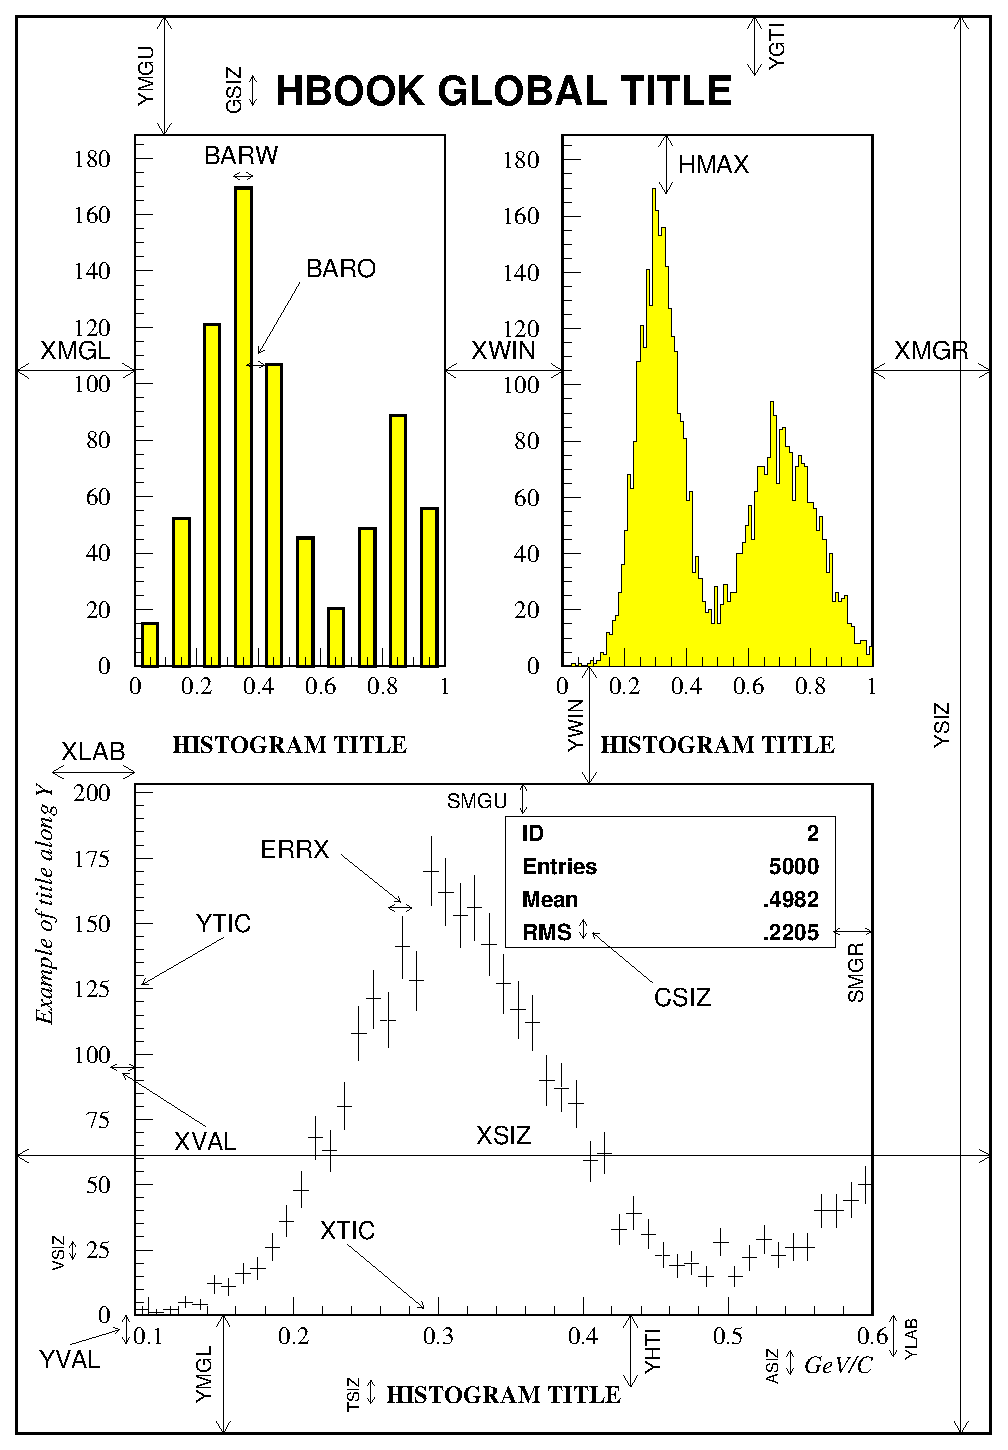
\includegraphics[width=.8\linewidth]{hplset.eps}
\caption{A graphical view of the {\tt SET} parameters}
\label{fig:HPLSET}
\end{figure}

\section{More on labels}
\index{alphanumeric!labels}
\index{label}

By default, labels used by \PAWcind{AXIS} and \PAWcind{PIE}
are numeric labels.
The command \PAWcind[LABELS]{GRAPHICS/PRIMITIVES/LABELS}
(or \PAWcind{LABELS} for short), allows the user to define
up to nine alphanumeric set of labels
(numbered from \texttt{1} to \texttt{9}).
These labels can then be used in subsequent commands
using \PAWcind{PIE} or \PAWcind{AXIS} primitives of HIGZ.

The \PAWcind{LABELS} command has three parameters:
\begin{DLtt}{123456}
\item[LABNUM] An integer between \texttt{1} and \texttt{9}.
              It identifies the labels set.
\item[NLABS]  The number of items to be placed on the labels 
              (up to \texttt{50}).
\item[CHLABS] \texttt{NLABS} character strings specifying the label items.
\end{DLtt}

The label sets thus defined can be used for axes on all plots produced
by PAW (HPLOT histograms, graphs, vectors drawing, etc.) via the
\PAWcind[SET]{SET NDVX (NDVY)} command.
\index{axis!divisions}
These commands have the following structure:

\subsection*{Example of \texttt{NXDV} specification}
\begin{alltt}
    SET \Ssind{NDVX} i            e.g. SET NDVX 512
{\rm or}
    SET \Ssind{NDVX} i.jk         e.g. SET NDVX 10.25
\end{alltt}

In the first case the number \texttt{i} contains
\texttt{100} times the 
number of secondary divisions plus the number of primary divisions.
(e.g. \texttt{512} means \texttt{12} primary and \texttt{5} secondary division. 
By adding \texttt{10000} times \texttt{N3} to \texttt{i} a third level of divisions
is available.
\index{divisions}

In the second case the number in front of the dot \texttt{(i)} indicates the total
number of divisions, the first digit following the dot \texttt{(j)} the label
identifier (\texttt{LABNUM}) (if this number is equal to \texttt{0} numeric labels
are drawn). The second digit after the \texttt{(k)} dot indicates the position 
where the \index{label!text justification} labels have to be drawn (i.e. the
{\em text justification} parameter, in this case \texttt{5}, indicating 
horizontally written text centered on the interval). Study figures 
\ref{fig:LABNDVX} and \ref{fig:LABNDVY} for details. These two figures show 
that the labels can be centered on the tick marks (\texttt{1} to \texttt{4}) or on 
the divisions (\texttt{5} to \texttt{8}). If the labels are centered on the tick 
marks, note that the number of items in the command \texttt{LABELS} must be equal
to the number of tick marks (which is equal to the number of divisions 
{\bf plus one}), otherwise the last alphanumeric label on the axis will be 
undefined. \index{tick marks}

By default, the number of primary divisions given by \PAWcind[SET]{SET NDVX n}, 
\PAWcind[SET]{SET NDVY n} or \PAWcind[SET]{SET NDVZ n} is optimized to have a 
reasonable labelling. The number of primary divisions is also optimized 
according the number of zones (command \PAWcind[ZONE]{ZONE}) i.e : 
along the X direction the number of primary divisions is divided by 
\texttt{the_number_of_X _zones} along the Y direction the number of primary 
divisions in divided by \texttt{(the_number_of_Y_zones)/2}.

If the number of divisions has to be exactly equal to the
number given by \PAWcind[SET]{SET NDVX n}, \PAWcind[SET]{SET NDVY n} or
\PAWcind[SET]{SET NDVZ n}, a negative value must be used i.e.:
\subsection*{Forcing an exact number of divisions}
\begin{alltt}
    SET \Ssind{NDVX} -i            e.g. SET NDVX -512
or
    SET \Ssind{NDVX} -i.jk         e.g. SET NDVX -10.25
\end{alltt}

For example to label each subsequent X-axis with the names of the
months of the year centered in the middle of each bin one can use:
\subsection*{Example of alphanumeric labels on an axis}
\begin{alltt}
PAW > \Ucom{LABEL 1 12 JAN FEB MAR APR MAY JUN JUL AUG SEP OCT NOV DEC}
PAW > \Ucom{SET NDVX -12.15}
\end{alltt}

\begin{figure}[p]
\centering\includegraphics[width=.74\linewidth]{ndvx.eps}
\caption{Example of labelling for horizontal axes}
\label{fig:LABNDVX}

\medskip

\centering\includegraphics[width=.74\linewidth]{ndvy.eps}
\caption{Example of labelling for vertical axes}
\label{fig:LABNDVY}
\end{figure}

\section{Colour, line width, and fill area in HPLOT}
\index{histogram!presentation}
\index{fill!area}
\index{colour}
\index{line!width}

The aspect of HPLOT pictures can be modified via the \texttt{xWID}, \texttt{xTYP}
and \texttt{xCOL} attributes, where \texttt{x} can be \texttt{H}, \texttt{B},
\texttt{P}, or \texttt{F}, defined as follows:
\begin{DLtt}{12}
\item[B] zone Box
\item[F] Function
\item[H] Histogram
\item[P] Page
\end{DLtt}

The values given to the parameters \Ssind{PTYP}, \Ssind{BTYP}, \Ssind{HTYP},
and \Ssind{FTYP} are the HIGZ fill area interior styles. Interior style
 provided by the basic graphics package (i.e. GKS) can be used (cf the
corresponding documentation) but in order to have the same result on all 
devices, numbers greater than \texttt{100} (HIGZ styles: \ref{fig:HATCH}) should
be used. Figure \ref{fig:BTYP} shows how to use the \texttt{xTYP} parameter. 

The parameters \Ssind{PCOL}, \Ssind{BCOL}, \Ssind{HCOL} and \Ssind{FCOL}
are equivalent to \Ssind{PTYP}, \Ssind{BTYP}, \Ssind{HTYP}, and \Ssind{FTYP}
respectively, but instead of changing the hatch style, they change the
colour of the same areas. It is possible to specify both the border and
the inside color for the Histogram, Box Page, and Function (\Ssind{HCOL}, 
\Ssind{BCOL}, \Ssind{PCOL}, \Ssind{FCOL}).
\subsection*{Example of \texttt{HCOL} specification}
\begin{alltt}
      Ex:
                  +---- 1 The Histogram is filled
                  |     0 Only the border is drawn 
                  |+--- Border color (here 2) if the histogram is filled
                  ||++- Inside color (here 3) if the histogram is filled
                  ||||  Border color if the histogram is not filled
                  ||||
                  VVVV
       SET  HCOL  1203  
\end{alltt}
The same mechanism is also available for \Ssind{FCOL}, \Ssind{BCOL} and 
\Ssind{PCOL}.

If \Ssind{PCOL}, \Ssind{BCOL}, \Ssind{HCOL} or \Ssind{FCOL} are between \texttt{1}
and \texttt{99}, then only the contour of the corresponding area is changed. 
If they are between \texttt{1001} and \texttt{1099}, then the surface is filled with
the colour determined by the corresponding fill area colour index (1 to 99).
If they are between \texttt{1199} and \texttt{1999}, then the surface is filled with
the colour determined by the corresponding fill area colour index (1 to 99)
and the border is drawn with the corresponding line color index (1 to 9).

If one of the \Ssind{*COL} is greater than 1000 the corresponding value of the
Fill Area Interior Style (for \Ssind{HTYP}, \Ssind{BTYP}, \Ssind{PTYP} or 
\Ssind{FTYP}) is automatically set to \texttt{1} (solid).

In addition, \Ssind{BCOL} has two digits after the dot. The first one specifies
the colour of the zone box shadowing and the second the colour
of the statistic box shadowing. 
\index{colour}

\section{Information about histograms}
\index{date!and hour on pictures}
\index{file name!on pictures}
\index{date}
\index{fit!parameters on pictures}
\index{statistic!parameters on pictures}

Four options are available to plot additional informations on HPLOT pictures:
\Oind{DATE}, \Oind{FILE}, \Oind{STAT} and \Oind{FIT}.

\begin{alltt}
PAW > \Ucom{OPTION DATE}        | Plot date and hour on current HPLOT picture
PAW > \Ucom{OPTION FILE}        | Plot file name of current histogram
PAW > \Ucom{OPTION STAT}        | Plot statistics of current histogram
PAW > \Ucom{OPTION FIT}         | Plot Fit parameters of current histogram
\end{alltt}

For each of these \PAWcind{OPTION} commands a corresponding 
\PAWcind{SET} parameter is available:

\begin{alltt}
PAW > \Ucom{SET DATE i}    | Default is 2
PAW > \Ucom{SET \Ssind{FILE} i}    | Default is 1
\end{alltt}
where \texttt{i} defines the position of the date or file name:

\begin{DLtt}{12345678}
\item[i = 1 :] Top left corner        of page/current histogram.
\item[i = 2 :] Top right corner
\item[i = 3 :] Bottom left corner
\item[i = 4 :] Bottom right corner
\end{DLtt}

For example the command:
\begin{alltt}
PAW > \Ucom{SET \Ssind{DATE} 3}
\end{alltt}
sets the position of the date to the bottom left corner of the HPLOT pictures.
\begin{alltt}
PAW > \Ucom{SET \Ssind{STAT} i}    | Default is 1111
\end{alltt}
where \texttt{i} corresponds to binary status bits \texttt{AOURMEI} as follows: 

\begin{DLtt}{1234}
\item[A=1] Draw the contents of all channels
\item[O=1] Draw number of overflows
\item[U=1] Draw number of underflows
\item[R=1] Draw R.M.S.
\item[M=1] Draw mean value
\item[E=1] Draw number of entries
\item[I=1] Draw histogram identifier
\end{DLtt}

For example the command:

\begin{alltt}
PAW > \Ucom{SET STAT 10}
\end{alltt}

sets the statistics informations to be only the number of entries.

\begin{alltt}
PAW > \Ucom{SET \Ssind{FIT} i}     | Default is 101
\end{alltt}
where \texttt{i} corresponds to binary status bits \texttt{CEP} as follows: 

\begin{DLtt}{123}
\item[C=1] Draw \(\chi^2\)
\item[E=1] Draw errors
\item[P=1] Draw fit parameters
\end{DLtt}

For example to draw only the result of the \(\chi^2\) fit one would use:
\begin{alltt}
PAW > \Ucom{SET FIT 100}
\end{alltt}

For all these \PAWcind{OPTION}s, the {\bf character size} is specified with the 
command \PAWcind[SET]{SET CSIZ} and the character font used with 
\PAWcind[SET]{SET CFON}.



\subsection*{Fill area style, marker and line type}

The Fill Area Interior Style, The Fill Area Style Index,
the Marker TYPe and the Line TYPe are set respectively using the
\PAWcind{IGSET} parameters
\Ssind{FAIS}, \Ssind{FASI}, \Ssind{MTYP} and \Ssind{LTYPE}.

\subsection*{Example}
\begin{alltt}
PAW > \Ucom{IGSET FAIS 3}      | Fill area are hatched
PAW > \Ucom{IGSET FASI 244}    |   with the style index
PAW > \Ucom{IGSET MTYP 25}     | Marker type is an empty square
PAW > \Ucom{IGSET LTYP 15}     | Line type is dotted
\end{alltt}
\index{hatch style}
\index{fill!area!style index}
\index{fill!area!interior style}
\index{marker!type}
\index{line!type}

HIGZ provides some portable fill area styles index coded
using three digits \texttt{ijk} as follows:

\begin{DLtt}{12}
\item[i:] Distance between each hatch in mm
\item[j:] Angle between \texttt{90} and \texttt{180} degrees
\item[k:] Angle between \texttt{0} and \texttt{90} degrees
\end{DLtt}

These numbers are coded according to table \ref{tab:HIGZSTY}
and examples are shown in figure \ref{fig:HATCH}.

\begin{table}
\[
\begin{array}{|crcrcr|}
\hline
\mbox{\tt i} &  \mathrm{Distance} &
\mbox{\tt j} &  \mathrm{Angle}    &
\mbox{\tt k} &  \mathrm{Angle}     \\
\hline
   &                               &
0  & 180^{\circ}                   &
0  &   0^{\circ}                   \\
1  & 0.75 \mathrm{mm}              &
1  & 170^{\circ}                   &
1  &  10^{\circ}                   \\
2  & 1.50 \mathrm{mm}              &
2  & 160^{\circ}                   &
2  &  20^{\circ}                   \\
3  & 2.25 \mathrm{mm}              &
3  & 150^{\circ}                   &
3  &  30^{\circ}                   \\
4  & 3.00 \mathrm{mm}              &
4  & 135^{\circ}                   &
4  &  45^{\circ}                   \\
5  & 3.75 \mathrm{mm}              &
5  & \multicolumn{1}{c}{\mbox{not drawn}} &
5  & \multicolumn{1}{c|}{\mbox{not drawn}} \\
6  & 4.50 \mathrm{mm}              &
6  & 120^{\circ}                   &
6  &  60^{\circ}                   \\
7  & 5.25 \mathrm{mm}              &
7  & 110^{\circ}                   &
7  &  70^{\circ}                   \\
8  & 6.00 \mathrm{mm}              &
8  & 100^{\circ}                   &
8  &  80^{\circ}                   \\
9  & 6.75 \mathrm{mm}              &
9  &  90^{\circ}                   &
9  &  90^{\circ}                   \\
\hline
\end{array}
\]
\caption{Codification for the HIGZ portable fill area interior styles}
\label{tab:HIGZSTY}
\end{table}

\subsection*{Example}
\begin{alltt}
PAW > \Ucom{IGSET FAIS 3}      | Fill area interior style is hatched
PAW > \Ucom{IGSET FASI 190}    | Hatch type is 190
\end{alltt}
These commands will yield hatching with two sets of lines
at $90^{\circ}$ and $0^{\circ}$ spaced 1 mm apart.

\begin{sidewaysfigure}
\begin{minipage}{.49\textheight}
\centering\includegraphics[height=14cm]{btyp.eps}
\caption{Usage of fill area types in HPLOT}
\label{fig:BTYP}
\end{minipage}\hfill
\begin{minipage}{.49\textheight}
\centering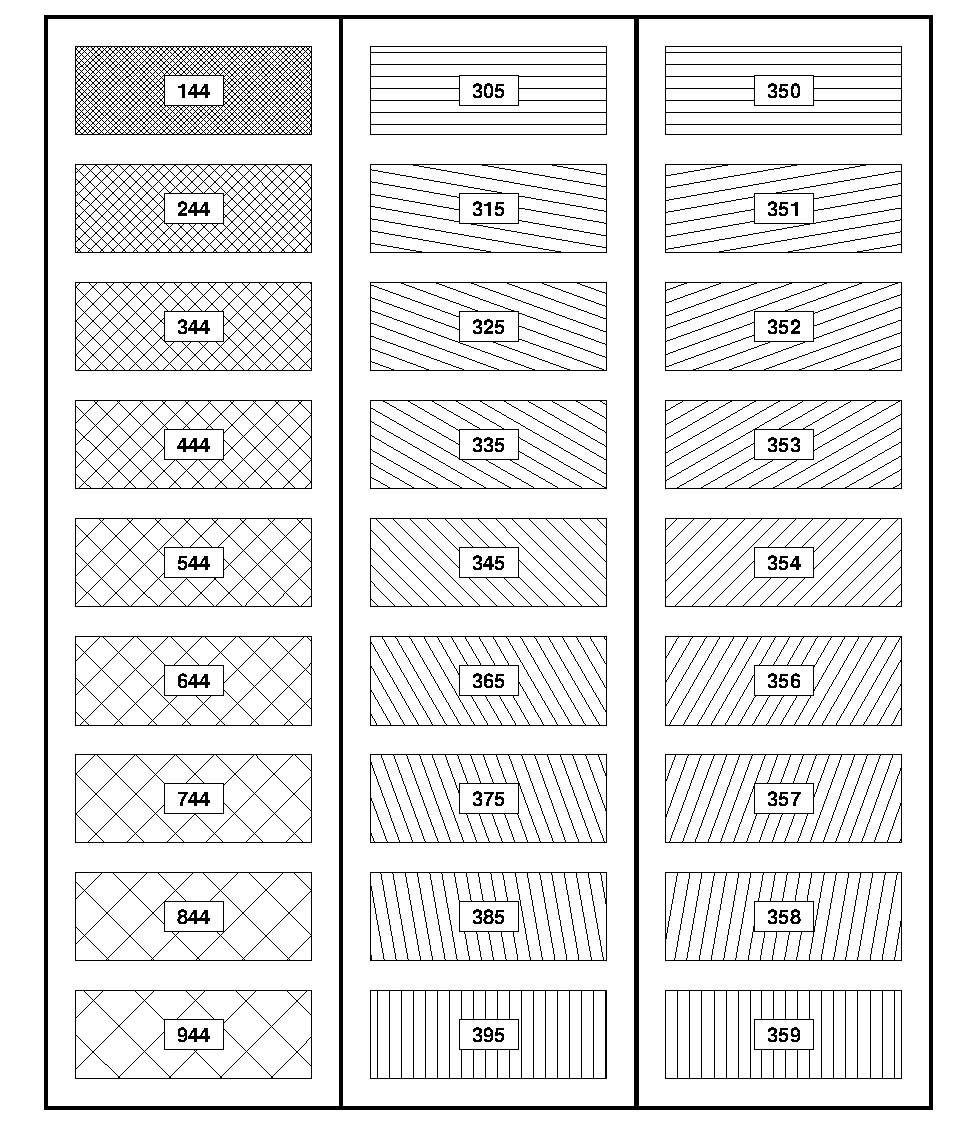
\includegraphics[height=14cm]{fasi.eps}
\caption{HIGZ portable hatch styles}
\label{fig:HATCH}
\index{hatch style}
\end{minipage}
\end{sidewaysfigure}

\begin{figure}[p]
\centering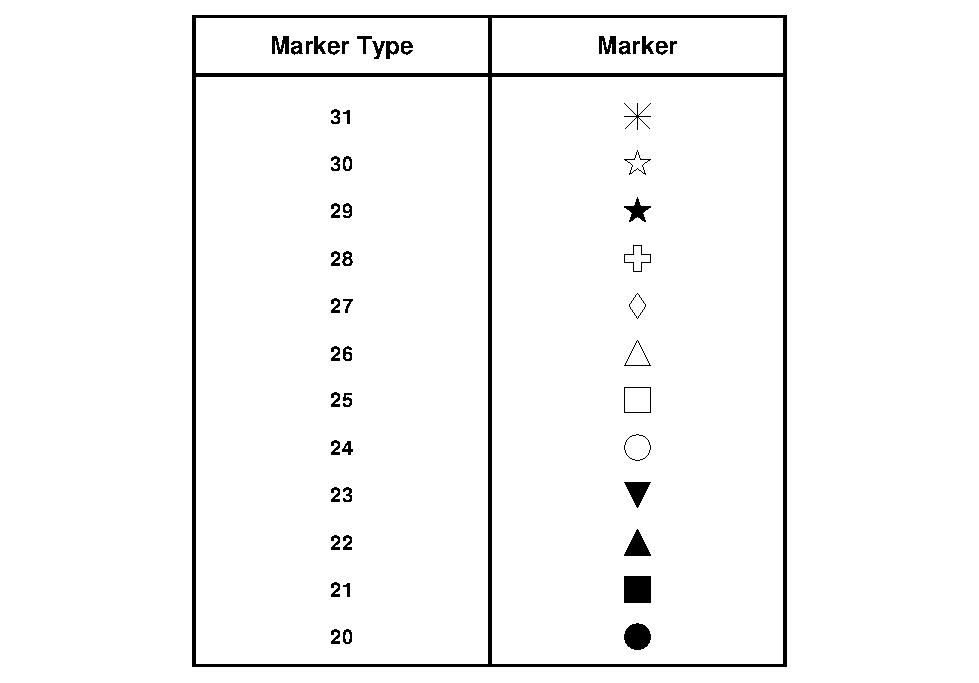
\includegraphics[width=12cm]{marker.eps}
\caption{HIGZ portable marker types}
\label{fig:MTYPE}
\index{marker!type}

\centering\includegraphics[width=10cm]{ltype.eps}
\caption{HIGZ portable line types}
\label{fig:LTYPE}
\index{line!type}

\centering\includegraphics[width=10cm]{greylev.eps}
\caption{PostScript grey level simulation of the basic colours}
\label{fig:GREYLEV}
\index{fonts}
\end{figure}

\section{Text drawing}
In PAW, text output can be produced in two ways:
\begin{enumerate}
\item {\em Automaticaly} with commands like \PAWcind{GRAPH} or 
      \PAWcind{HISTO/PLOT} in which a lot of text is drawn: the axis labels, the
      histogram title, the global title, the statistics etc. . The attributes
      (font, colour or size) and the placement of these texts are controled 
      with the command \PAWcind{SET}. In the rest of the chapter, the text
      produce {\em automaticaly} will be called {\em HPLOT text}
\item {\em Directly} with the commands \PAWcind{ITX} and \PAWcind{TEXT}. The 
      attributes of \PAWcind{ITX} are controlled with the command 
      \PAWcind{IGSET} whereas the attributes of \PAWcind{TEXT} are given
      with the command parameters.
\end{enumerate}

\subsection*{Text placement}
The text placement specify where the text must be drawn. For the
{\em HPLOT text}, the text position  is always in centimeters whereas for
\PAWcind{ITX} or \PAWcind{TEXT} the current coordinate system is used. 
\subsubsection{HPLOT text}
The possible text placements for {\em HPLOT text} are described in the
following example:
\begin{alltt}
PAW > \Ucom{SET XVAL 0.40} | distance between the Y axis and the axis values
PAW > \Ucom{SET YVAL 0.20} | distance between the X axis and the axis values
PAW > \Ucom{SET YLAB 0.80} | distance X axis to labels
PAW > \Ucom{SET XLAB 1.40} | distance Y axis to labels
PAW > \Ucom{SET YGTI 1.50} | Y position of global title
PAW > \Ucom{SET YHTI 1.20} | Y position  of histogram title
PAW > \Ucom{SET YNPG 0.60} | Y position for the page number
PAW > \Ucom{HISTO/PLOT 10} | the histogram 10 is drawn with previous settings
\end{alltt}
See figure \ref{fig:HPLSET} for more details.
\subsubsection{ITX}
In the command \PAWcind{ITX} the text position is defined with two mandatory
parameters (\texttt{X} and \texttt{Y}): 
\begin{alltt}
PAW > \Ucom{SELNT 1}         | cm coordinates
PAW > \Ucom{ITX 5 5 'Hello'} | 'Hello' is drawn at the position (5,5)
\end{alltt}
\subsubsection{TEXT}
In the command \PAWcind{TEXT} the text position is defined with two mandatory
parameters (\texttt{X} and \texttt{Y}): 
\begin{alltt}
PAW > \Ucom{SELNT 1}            | cm coordinates
PAW > \Ucom{TEXT 5 5 'Hello' 1} | 'Hello' is drawn at the position (5,5)
\end{alltt}

\subsection*{Text size}
For all the texts drawn with PAW commands, the text size is always specified
in centimeters.
\subsubsection{HPLOT text}
The possible text sizes for {\em HPLOT text} are described in the
following example:
\begin{alltt}
PAW > \Ucom{SET ASIZ 0.28} | axis label size
PAW > \Ucom{SET CSIZ 0.28} | comment size
PAW > \Ucom{SET GSIZ 0.28} | global title size
PAW > \Ucom{SET KSIZ 0.28} | Hershey character size
PAW > \Ucom{SET 2SIZ 0.28} | scatter plot and table character. size
PAW > \Ucom{SET TSIZ 0.28} | histogram title size
PAW > \Ucom{SET VSIZ 0.28} | axis values size
PAW > \Ucom{HISTO/PLOT 10} | the histogram 10 is drawn with previous settings
\end{alltt}
See figure \ref{fig:HPLSET} for more details.
\subsubsection{ITX}
The text character heigh attribute for use by future invocations of 
\PAWcind{ITX} is set using the \Ssind{CHHE} parameter as follows:
\begin{alltt}
PAW > \Ucom{IGSET CHHE 1}    | set the character heigh to 1 cm.
PAW > \Ucom{ITX 5 5 'Hello'} | the size of 'Hello' is 1 cm.
\end{alltt}
\subsubsection{TEXT}
In the command \PAWcind{TEXT} the text size is a mandatory parameter
(\texttt{SIZE}).
\begin{alltt}
PAW > \Ucom{TEXT 5 5 'Hello' 1} | the size of 'Hello' is 1 cm.
\end{alltt}

\subsection*{Text orientation}
The text orientation is an angle (in degrees) between the \texttt{X} axis
and the text axis. By default this angle is equal to 0.
\subsubsection{HPLOT text}
Text orientation cannot be changed with some \PAWcind{SET} parameters for the
{\em HPLOT text}. It is always automaticaly computed. For example in
the command \PAWcind{ATITLE}, which draws the axis titles, the title
on the \texttt{Y} axis is automaticaly drawn with an angle of 90 degrees.
\subsubsection{ITX}
The text orientation attribute for use by future invocations of 
\PAWcind{ITX} is set using the \Ssind{TANG} parameter as follows:
\begin{alltt}
PAW > \Ucom{IGSET TANG 90}   | set the text angle to 90 degrees.
PAW > \Ucom{ITX 5 5 'Hello'} | 'Hello' is drawn with an angle of 90 degrees.
\end{alltt}
\subsubsection{TEXT}
In the command \PAWcind{TEXT} the text orientation is an optional parameter
(\texttt{ANGLE}).
\begin{alltt}
PAW > \Ucom{TEXT 5 5 'Hello' ! 90} | 'Hello' is drawn with an angle of 90 degrees
\end{alltt}

\subsection*{Text alignment}
\index{text!alignment!horizontal}
\index{text!alignment!vertical}
The text alignment controls the placement of the character string  with 
respect to the specified text position.
\subsubsection{HPLOT text}
Text alignment cannot be changed for the
{\em HPLOT text}. It is automaticaly computed.
\subsubsection{ITX}
The text alignment attributes for use by future invocations of \PAWcind{ITX}
are set using the \Ssind{TXAL} parameter as follows:
\begin{alltt}
PAW > \Ucom{IGSET TXAL (10*(horizontal alignment) + (vertical alignment))}
\end{alltt}
The horizontal and 
vertical alignments parameters must be in the range \texttt{0-3}. The horizontal 
alignment specifies which end of the string (or its geometric center) is 
aligned with the specified point given in \PAWcind{ITX}.
The vertical alignment controls whether the top of tall characters
(or the bottom of capital letters) line up with the specified point 
(see figure \ref{fig:ALIGN}).
\begin{itemize}
\item[ITXALH] horizontal alignment
\begin{itemize}
\item[0] normal (usually same as 1)
\item[1] left end of string at specified point
\item[2] center of string at specified point
\item[3] right end of string at specified point
\end{itemize}
\item[ITXALH] vertical alignment
\begin{itemize}
\item[0] normal
\item[1] top of tallest chars plus any built in spacing
\item[2] top of tallest chars
\item[3] halfway between 2 and 4 
\end{itemize}
\end{itemize}
\begin{figure}
\centering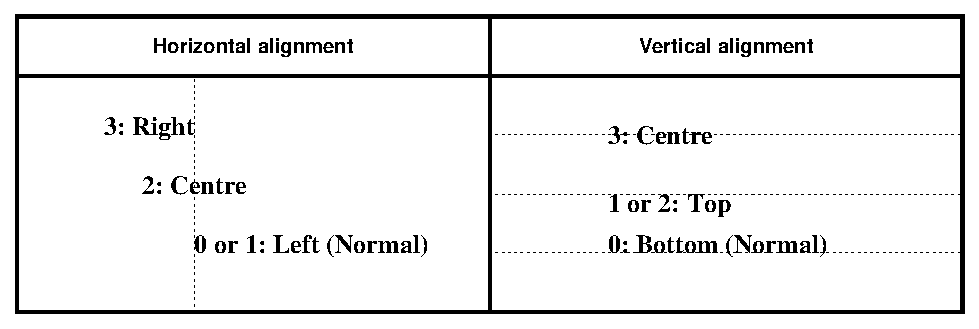
\includegraphics[width=12cm]{align.eps}
\caption{Text alignment}
\label{fig:ALIGN}
\index{text alignment}
\end{figure}
\begin{alltt}
PAW > \Ucom{IGSET TXAL 23}   | The horizontal and vertical alignments are centered
PAW > \Ucom{ITX 5 5 'Hello'} | 'Hello' is drawn center adjusted
\end{alltt}
\subsubsection{TEXT}
In the command \PAWcind{TEXT} the text alignment is an optional parameter
(\texttt{CHOPT}). Only the horizontal alignment can be changed among three 
possible values: Left, Center or Right.
\begin{alltt}
PAW > \Ucom{TEXT 5 5 'Hello' 1 ! L} | 'Hello' is drawn left adjusted (default)
PAW > \Ucom{TEXT 5 5 'Hello' 1 ! C} | 'Hello' is drawn center adjusted
PAW > \Ucom{TEXT 5 5 'Hello' 1 ! R} | 'Hello' is drawn right adjusted
\end{alltt}

\subsection*{Text colour}
The text colour is define via a colour index in the colour table.
\subsubsection{HPLOT text}
\begin{alltt}
PAW > \Ucom{SET XCOL 2}    | X axis color
PAW > \Ucom{SET YCOL 3}    | Y axis color
PAW > \Ucom{HISTO/PLOT 10} | the histogram 10 is drawn with previous settings
\end{alltt}
\subsubsection{ITX}
The text colour attribute for use by future invocations of 
\PAWcind{ITX} is set using the \Ssind{TXCI} parameter as follows:
\begin{alltt}
PAW > \Ucom{IGSET TXCI 3}    | set the text colour to green.
PAW > \Ucom{ITX 5 5 'Hello'} | 'Hello' is drawn in green.
\end{alltt}
\subsubsection{TEXT}
The text colour attribute for use by future invocations of 
\PAWcind{TEXT} is set using the \Ssind{TXCI} parameter as follows:
\begin{alltt}
PAW > \Ucom{IGSET TXCI 2}       | set the text colour to red.
PAW > \Ucom{TEXT 5 5 'Hello' !} | 'Hello' is drawn in red.
\end{alltt}

\subsection*{Text font and precision}
\index{font!text}
\index{text!font}
\index{text!precision}
\index{precision!text}
Text font selects the desired character font e.g. a roman font, a sans-serif 
font, etc. Text precision specifies how closely the graphics package 
implementation must follow the current size and orientation attributes. 
String (\texttt{0}) precision is most liberal (hardware), stroke (\texttt{2}) 
precision is most strict. Character precision is in the middle (\texttt{1}). 
The value of text font is dependent upon the basic graphics package used. 
However, font number \texttt{0}, with precision \texttt{2} is always available,
independently from the basic graphics package used.% (see figure \ref{fig:SOFT}).
Hardware characters are available with all the basic graphics packages. With
X11, a large variety of font is available. They are the same as the PostScript
fonts (see figure \ref{PS-FONT}).

\subsubsection{HPLOT text}
\begin{alltt}
PAW > \Ucom{SET CFON -60}  | comment font is Helvetica Bold
PAW > \Ucom{SET GFON -20}  | global title font is Times Bold
PAW > \Ucom{SET LFON -60}  | axis labels font is Helvetica Bold
PAW > \Ucom{SET TFON -20}  | general comments is Times Bold
PAW > \Ucom{SET VFON -60}  | axis values font is Helvetica Bold
PAW > \Ucom{HISTO/PLOT 10} | the histogram 10 is drawn with previous settings
\end{alltt}
Note that \texttt{SET *FON ffp} set all the {\em HPLOT text} font to the
same value \texttt{ffp}.

\subsubsection{ITX}
Text font and precision attributes for use by later
invocations of \PAWcind{ITX} are set with \Ssind{TXFP} as follows:
\begin{alltt}
PAW > \Ucom{IGSET TXFP (10*(Text font) + (text precision))}
\end{alltt}

\subsubsection{TEXT}
This command draws a software character text, independently from the basic
graphics package used by HIGZ. It can produce over 300 different graphic signs.
The way in which software characters are defined is via a string of valid
characters, intermixed by other characters, acting as ``escape'' characters
\index{character!escape} (e.g. a change of alphabet, upper or lower case). The
string is interpreted by \PAWcind{TEXT} and the resulting characters are 
defined according to the figure~\ref{SOFTTEXT}, which shows the list of 
available software characters. This command allows the user to mix different
types of characters (roman, greek, special, upper and lower case, sub and 
superscript). There are a total of 10 control characters.

\index{lower case letters}
\index{upper case letters}
\index{Greek letters}
\index{superscript}
\index{subscript}
\index{backspace}
\index{termination character}
\index{special symbols}
\label{ESCCHAR}
\begin{tabular}{||c|p{7cm}||c|p{7cm}||}
\hline
\multicolumn{4}{|c|}{\bf List of escape characters and their meaning}      \\
\hline
 $<$  & go to lower case                 & $>$  & go to upper case (default) \\
\hline
 \lsb & go to greek (Roman = default)    & \rsb & end of greek               \\
\hline
 "    & go to special symbols            & \#   & end of special symbols     \\
\hline
$\uparrow$  & go to superscript         & ?    & go to subscript            \\
\hline
 !    & go to normal level of script     & \&   & backspace one character    \\
\hline
 \$   & termination character (optional) &      &                            \\
\hline
\end{tabular}

Note that characters can be also entered directly in lower case or upper case
instead of using the control characters {\tt <} and {\tt >}.

The boldface characters may be simulated by setting the
attributes '\Sind{PASS}' and '\Sind{CSHI}' with \PAWcind{IGSET}.
The meaning of these attributes is the
following: Every stroke used to display the character is repeated
\Sind{PASS} times, at a distance (in percentage of the character height)
given by \Sind{CSHI}.

\begin{figure}
\centering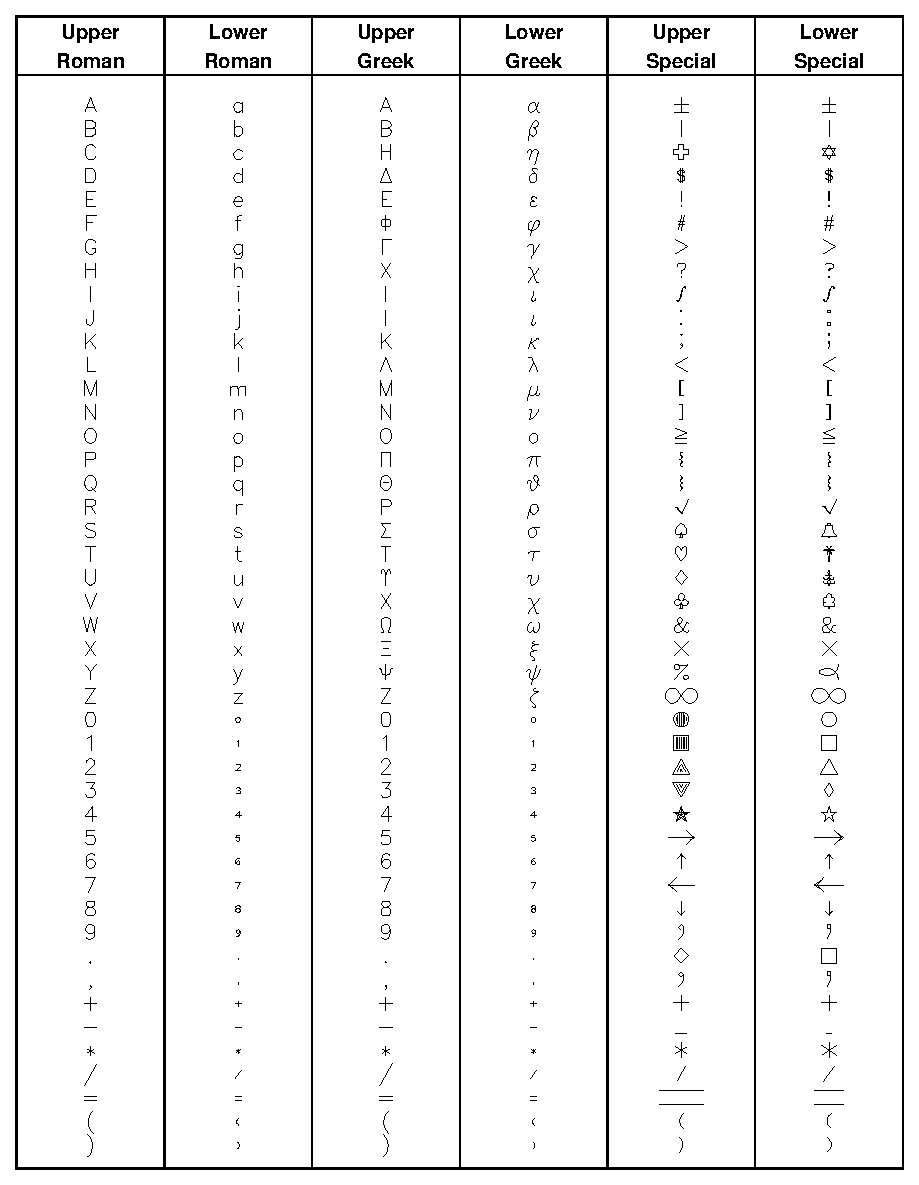
\includegraphics[width=.8\linewidth]{softtext.eps}
\caption{Characters available in \texttt{IGTEXT}}
\label{SOFTTEXT}
\end{figure}

\subsubsection{PostScript text fonts}
\index{font!PostScript}
\index{PostScript!fonts}
\index{PostScript!fonts!Times-Italic}
\index{PostScript!fonts!Times-Bold}
\index{PostScript!fonts!Times-BoldItalic}
\index{PostScript!fonts!Helvetica}
\index{PostScript!fonts!Helvetica-Oblique}
\index{PostScript!fonts!Helvetica-Bold}
\index{PostScript!fonts!Helvetica-BoldOblique}
\index{PostScript!fonts!Courier}
\index{PostScript!fonts!Courier-Oblique}
\index{PostScript!fonts!Courier-Bold}
\index{PostScript!fonts!Courier-BoldOblique}
\index{PostScript!fonts!Symbol}
\index{PostScript!fonts!Times-Roman}
\index{PostScript!fonts!ZapfDingbats}

PostScript files the text can be generated with PostScript fonts. The figure 
\ref{PS-FONT} shows all the PostScript fonts available on most PostScript 
printers. Note that the fonts {\tt -15} to {\tt -24} are the same than 
{\tt -1} to {\tt -14}, but they are drawn in hollow mode.

The correspondence between ASCII and {\sf ZapfDingbats} font
is given on figures \ref{PSTEXT1} and \ref{PSTEXT2}.
\PAWcind{TEXT} control characters are taken into account. In addition
the character $\sim$ switches to the {\sf ZapfDingbats} character set.
\index{lower case letters}
\index{upper case letters}
\index{Greek letters}
\index{superscript}
\index{subscript}
\index{backspace}
\index{termination character}
\index{special symbols}
\begin{center}
\begin{tabular}{||c|l||c|l||}
\hline
\multicolumn{4}{|c|}{\bf List of escape characters and their meaning}      \\
\hline
 $<$  & go to lower case (optional)      & $>$  & go to upper case (optional)\\
\hline
 \lsb & go to greek (Roman = default)    & \rsb & end of greek               \\
\hline
 "    & go to special symbols            & \#   & end of special symbols     \\
\hline
$\sim$ & go to ZapfDingbats               & \#   & end of ZapfDingbats        \\
\hline
$\uparrow$  & go to superscript          & ?    & go to subscript            \\
\hline
 !    & go to normal level of script     & \&   & backspace one character    \\
\hline
 \$   & termination character (optional) &      &                            \\
\hline
\end{tabular}
\end{center}
\par
The PostScript fonts can be used with precision {\tt 0} or precision {\tt 1}.
On the screen, a PostScript font used with precision {\tt 1} appears
like the \PAWcind{TEXT} characters, with precision 0 its appears as
hardware character (X11 fonts). In both cases the  PostScript file is the same.

Note that characters can also be entered directly in lower or upper case
instead of using the escape characters {\tt <} and {\tt >}.
Examples of PostScript text and math are shown in Figures~\ref{PSEX1}
and \ref{PSEX2}.

\begin{figure}
\begin{salltt}
PAW > IGSET LWID 6
PAW > BOX 0 16 0 5 
PAW > IGSET CHHE 0.5
PAW > IGSET TXAL 3
PAW > IGSET TXFP -130
PAW > ITX 3 4 'K\bs{}355nstler in den gr\bs{}345\bs{}373ten st\bs{}311dten
PAW > ITX 3 3 '\bs{}253\bs{}265 l''\bs{}372uvre on conna\bs{}333t l''artisan\bs{}273
PAW > ITX 3 2 '\bs{}(proverbe fran\bs{}321ais\bs{}
PAW > ITX 3 1 '\bs{}252\bs{}241Ma\bs{}337ana\bs{}41 \bs{}322ag&\bs{}306!das&\bs{}313!\bs{}272, dit l''\bs{}323l\bs{}325ve.
\end{salltt}
\begin{center}

\includegraphics[width=.7\linewidth]{psex1.eps}
\end{center}
\caption[PostScript text]
        {Example of PostScript text (result of input above)}
\label{PSEX1}

\bigskip

\begin{salltt}
PAW > IGSET LWID 6
PAW > BOX 0 16 0 5
PAW > IGSET CHHE 0.5
PAW > IGSET TXAL 23
PAW > IGSET TXFP -130
PAW > ITX 8 4 'e^+!e^-! "5# Z^o! "5# ll&^-!, qq&^\bs{}261!'
PAW > ITX 8 3 '| a&^[\bs{}256]! \bs{}267 b&^[\bs{}256]! | = [\bs{}345] a^i?&jk!+b^kj?&i'
PAW > ITX 8 2 'i ("d#?[m!y]&^\bs{}261![g^m]! + m [y]&^\bs{}261! ) = 0" r# (~r# + m^2!) [y] = 0'
PAW > ITX 8 1 'L?em! = e J^[m]?&em! A?[m]! , J^[m]?&em!=l&^\bs{}261![ g?m]!l , M^j?&i! = [\bs{}345&?a]! A?[a! t^a]j?&i! '
\end{salltt}
\begin{center}
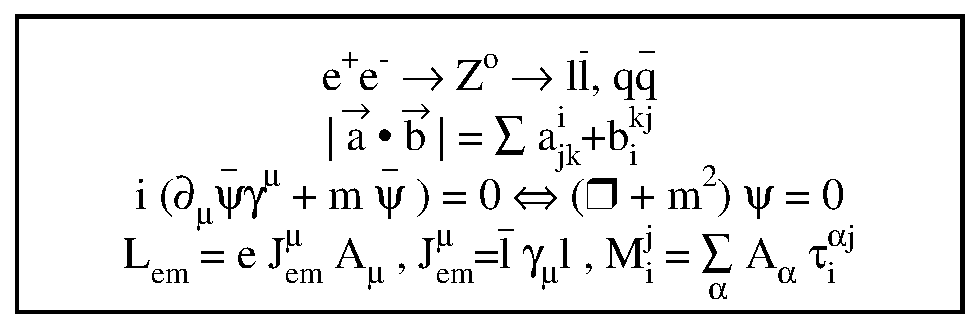
\includegraphics[width=.7\linewidth]{psex2.eps}
\end{center}
\caption[PostScript text and maths]%
        {Example of PostScript text and maths (result of input above)}
\label{PSEX2}
\end{figure}

\begin{figure}
\centering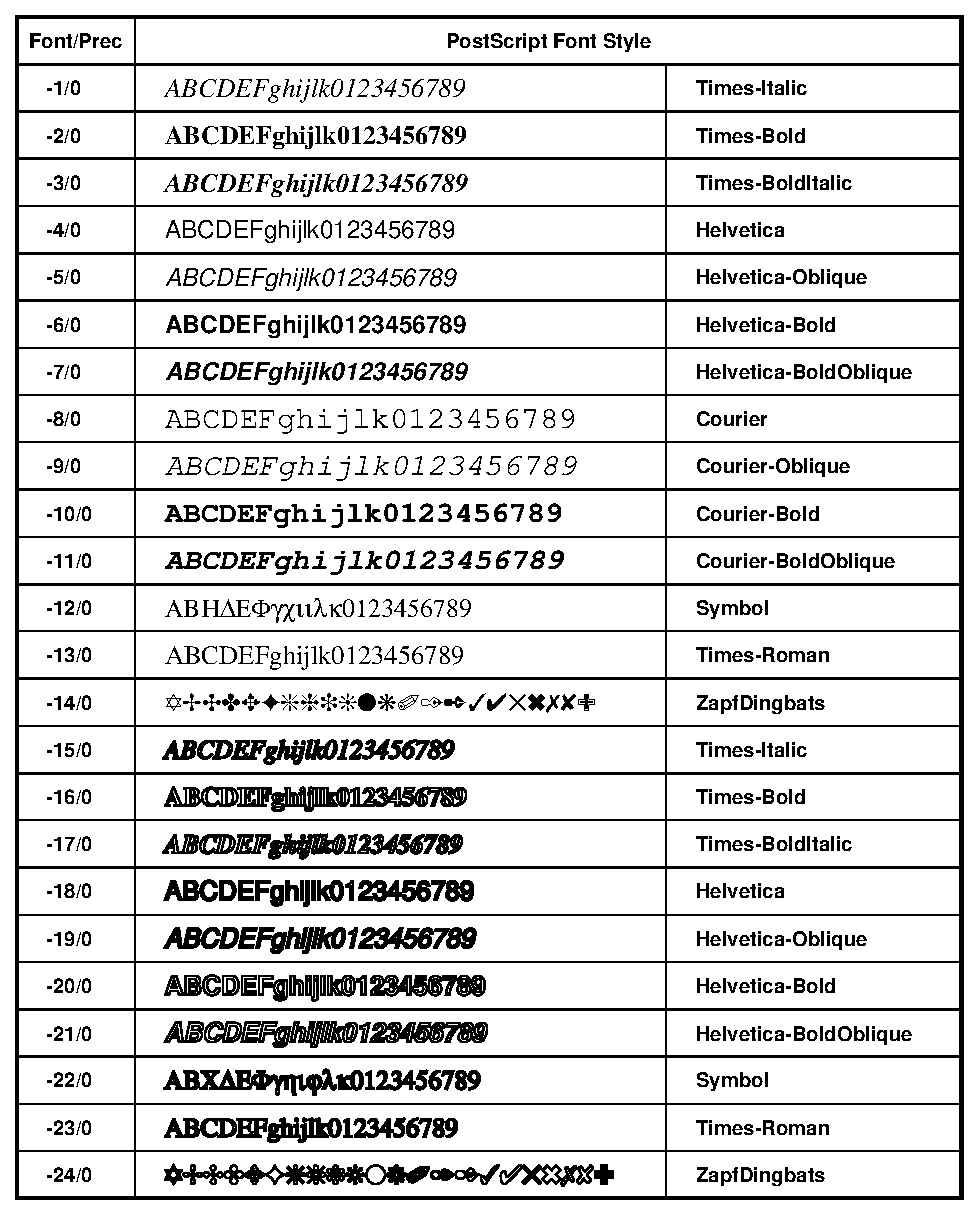
\includegraphics[width=\linewidth]{psfont.eps}
\caption{PostScript text fonts.}
\label{PS-FONT}
\end{figure}

\begin{figure}
\centering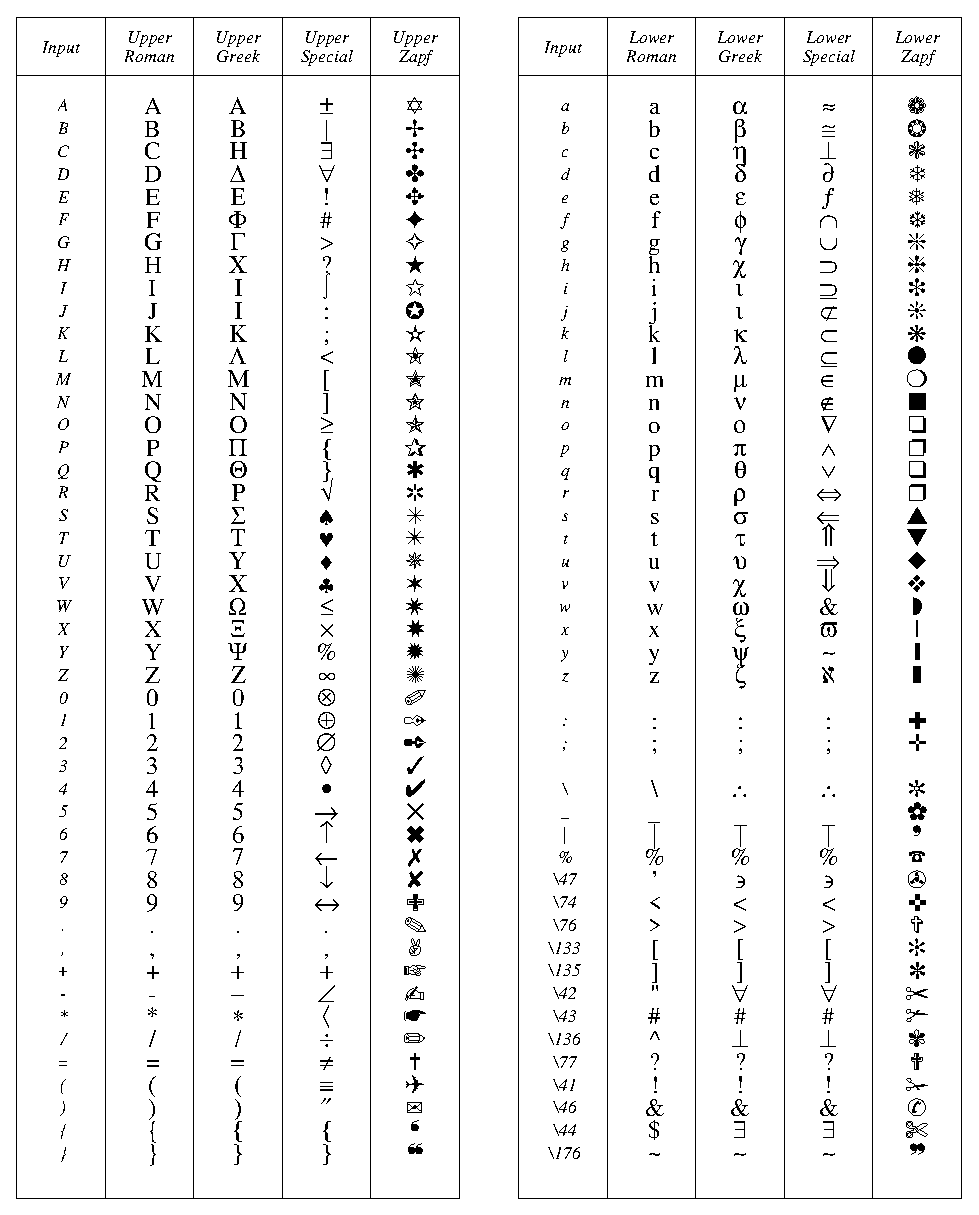
\includegraphics[width=\linewidth]{pstext1.eps}
\caption{PostScript characters (1).}
\label{PSTEXT1}
\end{figure}

\begin{figure}
\centering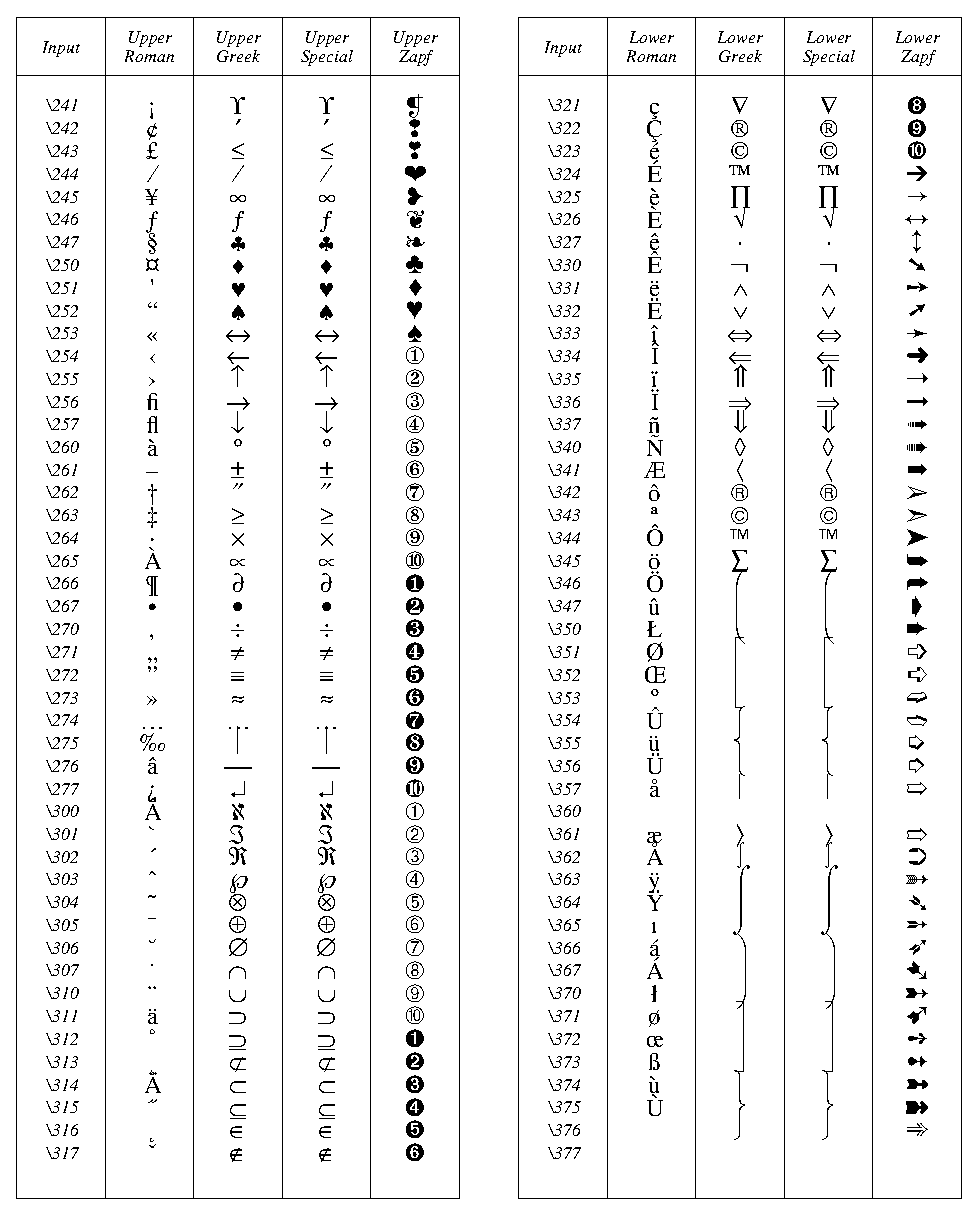
\includegraphics[width=\linewidth]{pstext2.eps}
\caption{PostScript characters (2).}
\label{PSTEXT2}
\end{figure}

\clearpage
\section{The HIGZ graphics editor}
\index{graphics!editor}
\index{editor}
\index{HIGZ!graphics editor}

The HIGZ pictures in memory can be modified interactively with the HIGZ
graphics editor. 
The command \PAWcind[MODIFY]{PICT/MODIFY} invokes the HIGZ editor
(see figure \ref{fig:GEDIFIG} for more details):
\begin{alltt}
PAW > \Ucom{PICT/MODIFY PNAME}
\end{alltt}
\texttt{PNAME} can be the complete name, the picture number in memory
or \texttt{' '}.

\begin{figure}
\includegraphics[width=\linewidth]{gedifig.eps}
\caption{The HIGZ graphics editor}
\label{fig:GEDIFIG}
\end{figure}

\endinput
%%%%%%%%%%%%%%%%%%%%%%%%%%%%%%%%%%%%%%%%%%%%%%%%%%%%%%%%%%%%%%%%%%%%%%%%%%%%%%%%
%                                                                              %
%   PAW   - Reference Manual -- LaTeX Source                                   %
%                                                                              %
%   Chapter 9: Distributed PAW                                                 %
%                                                                              %
%   Editor: Michel Goossens / IT-ASD                                           %
%   Last Mod.: 31 July 1998 Olivier Couet                                      %
%                                                                              %
%%%%%%%%%%%%%%%%%%%%%%%%%%%%%%%%%%%%%%%%%%%%%%%%%%%%%%%%%%%%%%%%%%%%%%%%%%%%%%%%

\chapter{Distributed PAW}
\label{sec:H1DIST}
 
\section{Access to remote files from a PAW session}
 
\index{remote!file}
\index{remote!shell}
\index{remote!login}
\index{RSHELL}
\index{RLOGIN}
When running PAW, it is often necessary to access files
(e.g. HBOOK files) which reside on a different computer. 
The ZFTP program described
above can be used if a very frequent access to the file is required. A
more convenient mechanism is the possibility to access the 
files directly. On many systems, one may now use \texttt{NFS}~\cite{bib-NFS}
for this purpose. Under some circumstances, for example if the HBOOK
file is not in exchange mode and it is to be accessed from a computer
running a different operating system, an alternate approach is required.
To fill this gap the PAW server is provided. This works using
a conventional Client/Server model. The client
(PAW) typically runs on a workstation. When the PAW command RLOGIN is invoked,
a PAW server is automatically started on the remote machine, normally
a mainframe or data server. 
 
Once the \texttt{RLOGIN REMOTE} command has been executed, the PAW Current Directory
is set to \texttt{//REMOTE}. The PAW client can now instruct the PAW server to
attach a file using the \texttt{RSHELL} command (e.g. \texttt{rshell file pawtest.dat}). If an
histogram with HBOOK ID=10 is on the remote file, than the PAW command
\texttt{Histo/Plot 10}
will plot this histogram on the local workstation. The histogram resides
on \texttt{//PAWC} like other histograms coming from local files.
 
The \texttt{RSHELL} command may be used to communicate with the PAW server.
The expression typed following \texttt{RSHELL} is passed to the server. The current
implementation of the PAW server recognizes the commands:
\begin{DLtt}{123456789012345678890}
\item[rshell file filename]Server connects filename
\item[rshell cdir //lun11] Server changes current directory
\item[rshell ld]           Server lists current directory
\item[rshell ld //]        Server lists all connected files
\item[rshell message]      Server pass message to operating system
\end{DLtt}
 
\subsection*{Access to remote files from a workstation}
\begin{alltt}
PAW > \Ucom{rlogin CERNVM}                         | connect to CERNVM
PAW > \Ucom{rshell file HRZTEST.DAT}               | PAW server connects HRZTEST DAT A to //LUN11
PAW > \Ucom{histo/plot 10}                         | plot histogram 10 from CERNVM
PAW > \Ucom{histo/fit 20 G}                        | fit histo 20 with a gaussian and plot it
PAW > \Ucom{rlogin VXCRNA}                         | connect to VXCRNA
PAW > \Ucom{rshell file DISK$DL:[PAW]HEXAM.DAT;3}  | PAW server on VXCRNA connects file to //LUN11
PAW > \Ucom{histo/plot 110}                        | plot histogram 110 from VXCRNA
PAW > \Ucom{rshell file HRZTEST.DAT}               | PAW server on VXCRNA connects file to //LUN12
PAW > \Ucom{histo/plot 110 s}                      | plot histogram 110 from HRZTEST.DAT
                                            | on VXCRNA on the existing picture
PAW > \Ucom{rshell ld //}                          | list all files connected on VXCRNA
PAW > \Ucom{cdir //CERNVM}                         | Change current PAW directory to CERNVM
PAW > \Ucom{histo/plot 110}                        | plot histogram 110 from CERNVM
PAW > \Ucom{histo/plot //VXCRNA/110}               | plot histogram 110 from VXCRNA
PAW > \Ucom{cdir //PAWC}                           | current directory to local memory
PAW > \Ucom{histo/list}                            | list all histograms in //PAWC
PAW > \Ucom{Histo/delete 0}                        | delete all histograms in memory
PAW > \Ucom{hrin //VXCRNA/0}                       | read all histograms from VXCRNA
                                            | file HRZTEST.DAT to //PAWC
PAW > \Ucom{cdir //CERNVM}                         | change directory to CERNVM
PAW > \Ucom{rshell file NEW.DAT.D 1024 N}          | creates a new file on the D disk
PAW > \Ucom{hrout 0}                               | write all histograms from //PAWC
                                            | to CERNVM file NEW DAT D
\end{alltt}
 
\newpage

\section{Using PAW as a presenter on VMS systems (global section)}
 
 
\index{global!section}
\index{VMS}
\index{presenter}
In addition to the facilities described in the previous section,
the standard version of PAW may be used as an online presenter
on VMS systems using the mechanism of global sections.
It is possible for two processes to reference the same histograms
using {\bf global sections}.
\index{global!section}
\index{VAX/VMS}
For example, the first process may be a {\bf histogram producer}
(e.g. a monitoring task) and the second process  {\bf PAW}.
As the
histograms are being gradually filled by the first task, PAW can
view them, and even reset them.
To use the global sections, it is also necessary to "page align" the common
which is in the global section. This is achieved in the "link step" when making
the process (see example).
The relevant statements are \texttt{SYS\$INPUT/OPTIONS}
to tell the linker that some options follow the link statement,
and \texttt{PSECT=PAWC,PAGE} which is the option to
page align the \texttt{/PAWC/} common.
 
\begin{minipage}{.48\textwidth}
\begin{alltt}
      PROGRAM PRODUCE
      PARAMETER MAXPAGES=100
      COMMON/PAWC/IPAWC(128*MAXPAGES)
      CHARACTER*8 GNAME
      INTEGER*4 HCREATEG
*
      GNAME='GTEST'
      WAIT_TIME=1.
      NUMEVT=1000
*...............           Create Global section
      NPAGES=HCREATEG(GNAME,IPAWC,128*MAXPAGES)
      IF(NPAGES.GT.0) THEN
         PRINT 1000,GNAME
 1000    FORMAT(' Global Section: ',A,' created')
      ELSE
         IERROR=-NPAGES
         PRINT 2000,IERROR
 2000    FORMAT(' Global Section Error', I6)
         GO TO 99
      ENDIF
      CALL HLIMIT(128*NPAGES)
*...............           Book histos.
      CALL HBOOK1(10,'Test1$',50,-4.,4.,0.)
      CALL HBOOK1(20,'Test2$',50,-4.,4.,0.)
*...............           Fill histos.
      DO 20 I=1,NUMEVT
         DO 10 J=1,100
            CALL RANNOR(A,B)
            CALL HFILL(10,A,0.,1.)
            CALL HFILL(20,B,0.,1.)
 10      CONTINUE
        CALL LIB$WAIT(WAIT_TIME)
 20   CONTINUE
*
 99   STOP
      END
 
$ fort produce
$ link produce,SYS$INPUT/OPTIONS,-
cern$library:packlib/lib,kernlib/lib
PSECT=PAWC,PAGE
\end{alltt}
\end{minipage}\hfill
\begin{minipage}{.50\textwidth}
\begin{alltt}
    PAW > \Ucom{edit produce}
       macro produce ntimes=100
         nt=[ntimes]
         zone 1 2
         histo/plot 10 K
         histo/plot 20 K
       loop:
           histo/plot 10 U
           histo/plot 20 U
           wait ' ' 1
           nt=[nt] -1
           if nt>0 goto loop
       return
    PAW > \Ucom{global GTEST}
    PAW > \Ucom{exec produce ntimes=20}
\end{alltt}
\includegraphics[width=\textwidth]{pawglob.eps}
\end{minipage}
\newpage

\section{Using PAW as a presenter on OS9 systems}
 
\index{presenter}
\index{OS9}
\index{TCP/IP}
\index{remote!login}
\index{remote!shell}
\index{RLOGIN}
\index{RSHELL}
\index{client}
\index{server}
\index{PAW!server}
The technique described in previous sections may also be used
to access HBOOK histograms being filled by a monitoring task
on OS9 systems from a standard PAW session running
on a machine with the TCP/IP software.
 
\begin{minipage}{.48\textwidth}
\begin{alltt}
      INDIRECT PAWC
      PROGRAM PRODUCE
*
*        Monitoring task MT1 in processor OP2.
*
      PARAMETER NWPAW=10000
      COMMON/PAWC/IPAWC(NWPAW)
*
      CALL HLIMIT(NWPAW)
*
*       Book histos.
*
      CALL HBOOK1(10,'TEST1$',50,-3.,3.,0.)
      CALL HBOOK1(20,'TEST2$',50,-3.,3.,0.)
*
*       Fill histos.
*
      NUMEVT=10000
      DO 20 I=1,NUMEVT
         DO 10 J=1,100
            CALL RANNOR(A,B)
            CALL HFILL(10,A,0.,1.)
            CALL HFILL(20,B,0.,1.)
 10      CONTINUE
 20   CONTINUE
*
 99   STOP
      END
\end{alltt}
\end{minipage}\hfill
\begin{minipage}{.50\textwidth}
\epsfig{file=pawos9.eps,width=\the\textwidth}
\end{minipage}
\bigskip
 
\subsection*{Example of how to access OS9 modules from PAW}
\begin{alltt}
PAW > \Ucom{rlogin O-OPAL01}                            | connect to an OS9 machine
PAW > \Ucom{rshell module OP2/MT1}                      | PAW server connects to OP2/MT1
                                                 | (Processor OP2, Monitoring Task MT1)
PAW > \Ucom{histo/plot 10}                              | plot histogram 10
PAW > \Ucom{hrin 0}                                     | read all histograms into //PAWC
PAW > \Ucom{Histo/File 1 local.dat 1024 N}              | create a new file local.dat
                                                 | on the client machine
PAW > \Ucom{hrout 0}                                    | save all histograms from //PAWC
                                                 | to the local file
PAW > \Ucom{rshell module OP3/MT2}                      | PAW server connects to another
                                                 | OS9 monitoring task
PAW > \Ucom{Output 56 os9.listing}                      | Change output file on client
PAW > \Ucom{rshell ldir}                                | list all histograms in MT2
                                                 | on file os9.listing
PAW > \Ucom{Output -56 }                                | Change output file to default (unit 6)
                                                 | file os9.listing is closed
\end{alltt}
\endinput

%%%%%%%%% Some commands for including PAW++ EPS screen dumps %%%%%%%%%%%%%%%%%%%

\newenvironment{ICON}[1]{\begin{minipage}{.1\textwidth}
                          \includegraphics[width=\textwidth]{pawpp#1.eps}
                          \end{minipage}\hfill
                          \begin{minipage}{.85\textwidth}}%
                          {\end{minipage}}
\newlength{\Mylen}
\newenvironment{PAWf}[2][.3]
               {\setlength{\Mylen}{.95\textwidth-\textwidth*\real{#1}}%
               \begin{minipage}{#1\textwidth}
               \includegraphics[width=\textwidth]{pawpp#2.eps}
               \end{minipage}\hfill
               \begin{minipage}{\Mylen}}%
               {\end{minipage}}
\newenvironment{PAWfR}[1]{\begin{minipage}{.3\textwidth}
                    \includegraphics[height=\textwidth,angle=90]{pawpp#1.eps}%
                          \end{minipage}\hfill
                          \begin{minipage}{.65\textwidth}}%
                          {\end{minipage}}
\newcommand{\PAWF}[2][1.]{\begin{center}
                      \includegraphics[width=#1\textwidth]{pawpp#2.eps}
                      \end{center}}
\newcommand{\PAWFR}[2][1.]{%
       \includegraphics[angle=90,width=#1\textwidth]{pawpp#2.eps}}


%%%%%%%%%%%%%%%%%% Zapf dingbats enumerate environments %%%%%%%%%%%%%%%%%%%%%%%%

\newcommand{\Denslist}
{\itemsep=0pt\parsep=0pt\partopsep=0pt\topsep=\baselineskip\parskip=0pt}
\newenvironment{EnumZW}{\renewcommand{\labelenumi}
                       {\setcounter{Mycount}{191+\value{enumi}}%
                       \raisebox{-2pt}[0cm][0cm]
                       {\Large\ding{\the\value{Mycount}}}}%
                       \enumerate\Denslist}%
                       {\endlist}
\newenvironment{EnumZB}{\renewcommand{\labelenumi}
                      {\setcounter{Mycount}{201+\value{enumi}}%
                   \raisebox{-2pt}[0cm][0cm]{\Large\ding{\the\value{Mycount}}}}%
                        \enumerate\Denslist}%
                       {\endlist}

%%%%%%% Description lists using sans serif font for term %%%%%%%%%%%%%%%%%%%%%%%

\newenvironment{DLsf}[1]% The parameter is the width of the term
                        {\def\DLH{\sf}\begin{DLgen}{#1}}{\end{DLgen}}
\newenvironment{DLsfc}[1]% The parameter is the width of the term
                        {\def\DLH{\sf}\begin{DLgenc}{#1}}{\end{DLgenc}}

%%%%%%%%% Specific commands for tagging PAW++ elements %%%%%%%%%%%%%%%%%%%%%%%%%

\newcommand{\NbDW}[1]{\setcounter{Mycount}{191+#1}\ding{\the\value{Mycount}}}%
\newcommand{\NbDB}[1]{\setcounter{Mycount}{201+#1}\ding{\the\value{Mycount}}}%
\newcommand{\Button}[1]{\psboxit{rectcartouche}{\spbox{\footnotesize\sf#1}}}
\newcommand{\Field}[1]{\psboxit{box 0.9 setgray fill}
                      {\spbox{\footnotesize\sf#1}}}

%%%%%%%%%%%%%%%%%%%%%%%%%%%%%%%%%%%%%%%%%%%%%%%%%%%%%%%%%%%%%%%%%%%%%%%%%%%%%%%%
\long\def\psboxit#1#2{%
\begingroup\setbox0=\hbox{#2}%
\dimen0=\ht0 \advance\dimen0 by \dp0%
    % Write out the PS code to set the current path using HEIGHT,
    % WIDTH , DEPTH of box0.
    \hbox{%
    \special{ps: gsave currentpoint translate
        0
        \number\dp0 \space 15800 div    % hand tuned for dvips
        \number\wd0 \space 15800 div    % hand tuned for dvips
        \number\ht0 \space -15800 div   % hand tuned for dvips
        #1 grestore}%
    \copy0%
}%HBOX
\endgroup%
}%

\long\def\spbox#1{\begingroup\fboxsep=1pt\leavevmode\setbox1\hbox{#1}%
    \dimen0\fboxrule \advance\dimen0 \fboxsep%
    \advance\dimen0 \dp1%
    \hbox{\lower \dimen0\hbox%
    {\vbox{\hrule height \fboxrule width 0pt%
          \hbox{\vrule width \fboxrule height 0pt \hskip\fboxsep%
          \vbox{\vskip\fboxsep \box1\vskip\fboxsep}\hskip%
                 \fboxsep\vrule width \fboxrule height 0pt}%
                 \hrule height \fboxrule width 0pt}}}\endgroup}%
\long\def\PScommands{\special{! TeXDict begin
/box{%                  Processes the path of a rectangle.
%                       Needs : x0 y0 x1 y1.
newpath 2 copy moveto 3 copy pop exch lineto 4 copy pop pop
lineto exch pop exch pop lineto closepath } bind def
%
/roundedbox{%           Processes the path of a rounded rectangle.
/radius exch store
3 2 roll %              x0 x1 y1 y0
2 copy min radius sub /miny exch store max radius add /maxy exch store
2 copy min radius sub /minx exch store max radius add /maxx exch store
newpath
minx radius add miny moveto
maxx miny maxx maxy radius arcto
maxx maxy minx maxy radius arcto
minx maxy minx miny radius arcto
minx miny maxx miny radius arcto 16 {pop} repeat
closepath
}bind def
%
/rectcartouche{%        Draws a filled and framed box
%                       Needs : x0 y0 x1 y1
4 copy .9 setgray 3 setlinewidth box fill .5 setgray box stroke
}bind def
%
/cartouche{%            Draws a filled and framed rounded box
%                       Needs : x0 y0 x1 y1 radius
5 copy .9 setgray 5 setlinewidth roundedbox fill .95 setgray roundedbox stroke
}bind def
%
end }%                  Closes dictionnary
}%
%
\PScommands
%
\renewcommand{\CERNLIB}{\textsc{cernlib}\index{CERNLIB}}
\renewcommand{\CMZ}{\textsc{cmz}\index{CMZ}}
\renewcommand{\COMIS}{\textsc{comis}\index{COMIS}}
\renewcommand{\CSPACK}{\textsc{cspack}\index{CSPACK}}
\renewcommand{\FATMEN}{\textsc{fatmen}\index{FATMEN}}
\renewcommand{\GEANT}{\textsc{geant}\index{GEANT}}
\renewcommand{\GKS}{\textsc{gks}\index{GKS}}
\renewcommand{\HBOOK}{\textsc{hbook}\index{HBOOK}}
\renewcommand{\HEPDB}{\textsc{hepdb}\index{HEPDB}}
\renewcommand{\HIGZ}{\textsc{higz}\index{HIGZ}}
\renewcommand{\HPLOT}{\textsc{hplot}\index{HPLOT}}
\renewcommand{\KUIP}{\textsc{kuip}\index{KUIP}}
\renewcommand{\MINUIT}{\textsc{minuit}\index{MINUIT}}
\renewcommand{\PATCHY}{\textsc{patchy}\index{PATCHY}}
\renewcommand{\PAW}{\textsc{paw}\index{PAW}}
\renewcommand{\SIGMA}{\textsc{sigma}\index{SIGMA}}
\renewcommand{\PAWPP}{\textsc{paw++}\index{PAW++}}
\renewcommand{\WWW}{\textsc{www}\index{WWW}}
\renewcommand{\VAXTAP}{\textsc{vaxtap}\index{VAXTAP}}
\renewcommand{\ZEBRA}{\textsc{zebra}\index{ZEBRA}}

%%%%%%%%%%%%%%%%%%%%%%%%%%%%%%%%%%%%%%%%%%%%%%%%%%%%%%%%%%%%%%%%%%%%%%%%%%%%%%%%

\chapter{PAW++: A guided tour}

\PAWPP{} is a powerful OSF/\MOTIF{} based Graphical User Interface to
the popular Physics Analysis Workstation \XPAW.  The graphical user interface
makes the full and rich command set of \XPAW{} available to even the naive
user. Simple point and click operations are enough to execute commands that
were previously accessable only to expert users.
Figure~\vref{fig:paw++} compares the functionalities of basic PAW with
PAW++.

\begin{figure}[H]
\centering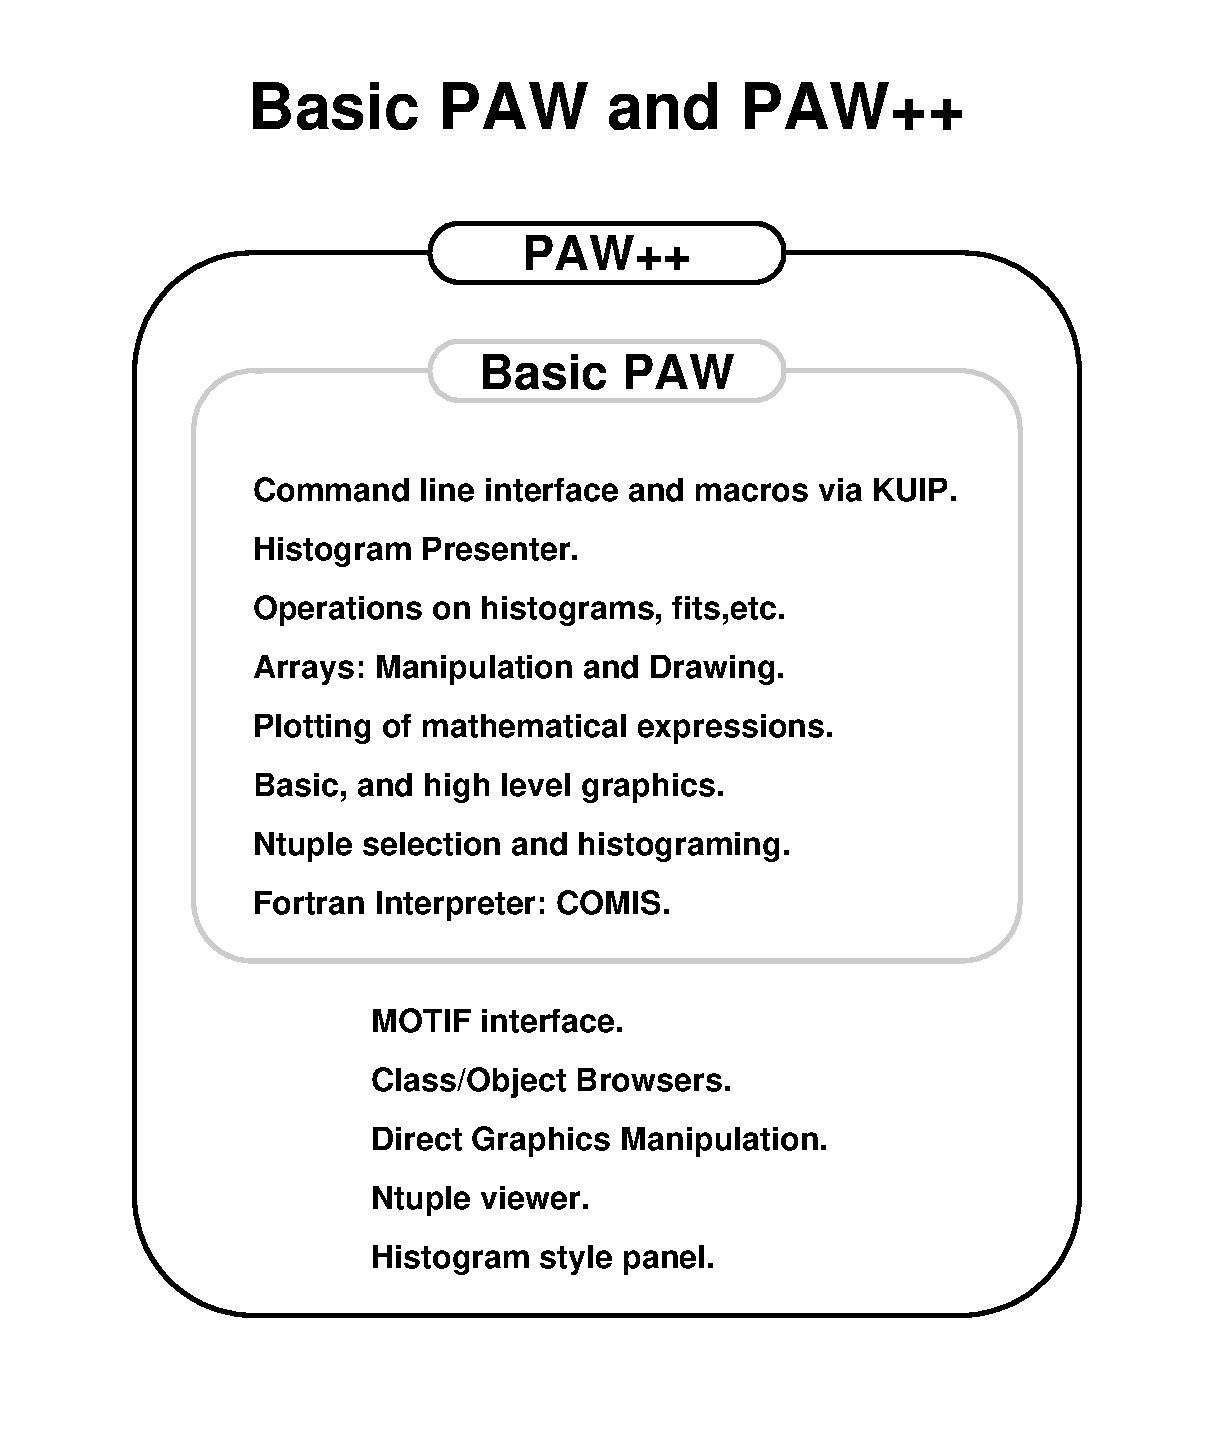
\includegraphics[width=.8\linewidth]{pawtut02.eps}
\caption{PAW and PAW++ compared}
\label{fig:paw++}
\end{figure}

At present \PAWPP{} is available on Unix workstations and VAX/VMS.

\PAWPP{} has, in addition to the conventional command line and macro types of
interface, the following dialogue modes:

\begin{DL}{Histogram style panel}
\item[Pull Down menus] They are useful to understand the command structure of
      the \XPAW{} system.
\item[Command panels] They give a ``panel representation'' of the commands.
\item[Object Browser] This is in many ways similar to the well-known browsers
      in the PC/MAC utilities or the visual tools on some workstations.
\item[Direct graphics] One can click in the graphics area and identify
      automatically which object has been selected. A pop-up menu appears
      with a list of possible actions on this object. For example, by clicking
      with the right mouse button on a histogram, one can make directly a
      gaussian fit, a smoothing etc.
      Pop-up menus are available by clicking on the \GW{} to
      automatically produce PostScript, Encapsulated PostScript, \LaTeX{} files
      or print the picture on your local printer.
\item[\HSP] Buttons are available to change
      histogram attributes, colours, line styles, fonts, and
      axes representation.
      2-D histograms can be rotated interactively. Zooming and rebinning can
      be performed interactively in real time.
\item[\NV] Just click on the Ntuple column name to histogram
      the column.
\end{DL}


The new system is largely self-explanatory. Only a subset of \XPAW{} has been
converted to this new user interface, but work is currently in progress to
offer many new facilities in future releases.

On all system on which \CERNLIB{} is installed, it is enough to type
\Ucom{paw++} to enter the system.

\PAWPP{} starts up with three windows on the screen:

\begin{DL}{The ``\PAWPP{} \EW''}
\item[The ``\PAWPP{} \EW'']
   includes a menu bar, a \TP, a current working directory indicator and an \IP.

\item[The ``\PAWPP{} Graphics 1'']
   window displays the graphics output from \HIGZ/\Xxi.
   Objects, e.g. histograms, displayed in the \GW{} can be
   manipulated by pointing at them, pressing the right mouse button and
   selecting an operation from the popup menu. Pointing at the edge of the
   \GW{} (between displayed object and window border) brings up a
   general popup menu. Up to 4 additional \GW{} can be opened by
   selecting ``Open New Window'' from this menu.

\item[The ``\PAWPP{} \MB'']
   displays all browsable classes and connected
   hbook files. Up to 4 additional browsers can be opened via the ``View'' menu
   of the ``\PAWPP{} \EW'' or via the ``Clone'' button on the
   browsers. For more information on the browsers see the ``Help'' menus.
\end{DL}


Figures~\ref{fig-pawppoverview1} on page \pageref{fig-pawppoverview1}
and \ref{fig-pawppoverview2} on page \pageref{fig-pawppoverview2} give
a detailed overview of the various windows of PAW++.

\begin{figure}[p]
\begin{center}
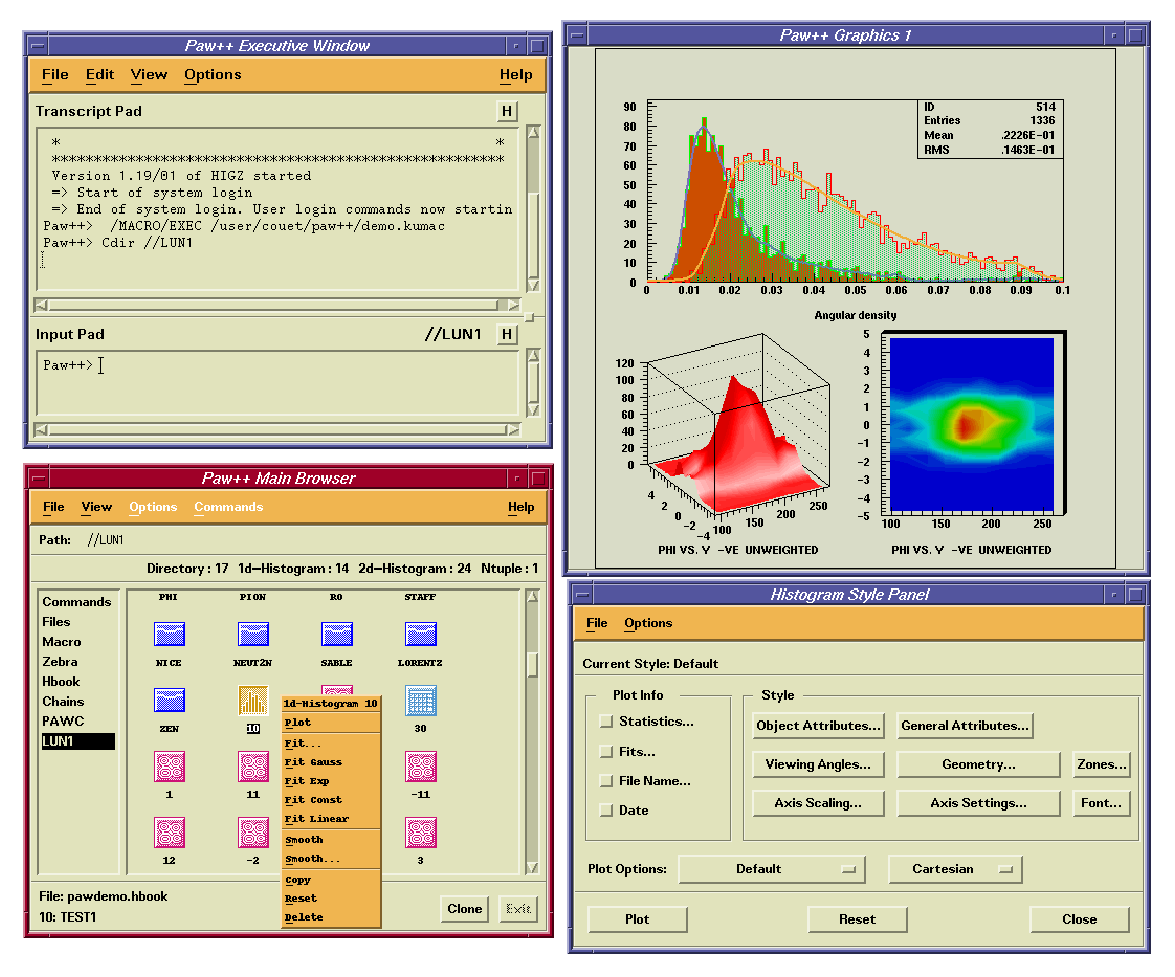
\includegraphics[width=\linewidth]{pawppoverview1.eps}
\end{center}
\small
\begin{UL}
\item The upper left corner is the \PAWPP{} \EW, with its \IP{}
      at the bottom and the \TP{} at the top.
\item The \PAWPP{} Browser, where the various entities (pictures, 1-D and
      2-D histograms and Ntuples) are all defined with their own symbol,
      is shown bottom left.  A ``pop-up'' menu has been activated for the 
      chosen 1-D histogram. Several actions like \texttt{Plot}, \texttt{Smooth},
      \texttt{Fit} etc... can be performed via this menu.
\item The \GW{} is seen top right. 
      A 1-D view of the data points and two 2-D views (a Surface-plot and a 
      colored contour plot) are shown.
      On the 1-D view, two 1-D histograms are 
      superimposed. The results of a ``smoothing'' type of fit to the data 
      points is also drawn. Information about the data and the fit can be found
      in the inserted window.
\item The \HSP{} at the lower right allows graphics
      attributes of the histogram to be controlled.
\end{UL}
\caption{PAW++ windows explained (I)}
\label{fig-pawppoverview1}
\end{figure}

\begin{figure}[p]
\begin{center}
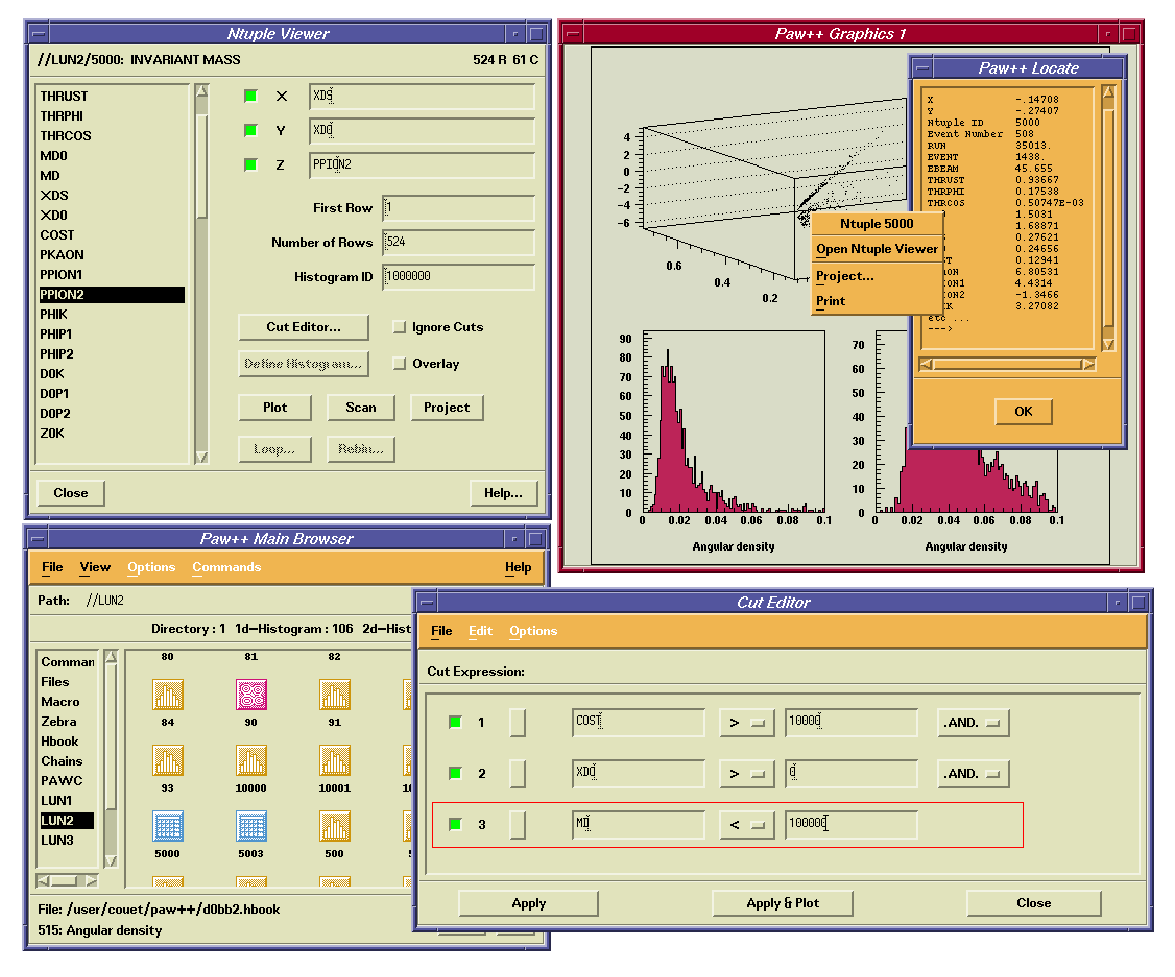
\includegraphics[width=\linewidth]{pawppoverview2.eps}
\end{center}
\small
\begin{UL}
\item The upper left corner shows the \NV.
      The left window shows the name of the various variables, characterizing
      the selected Ntuple. Other windows and press-buttons specify which
      combinations of the various variables and which events
      have to be treated (plotted, scanned, \ldots).
\item The lower left contains the \PAWPP{} Browser, with this time an Ntuple
      selected. A double on a Ntuple icon
      open automatically the \NV{} on the active Ntuple.
\item The \GW{} is seen top right and shows a 3-D view
      of the combination of three variables, whose cuts are
      specified with the \CE{} (see below).
\item Direct graphics interactions with Ntuple data are possible. Just
      by clicking on a point in the  \GW, the event description is displayed
      in the \PL{} window.
\item The \CE{} panel, shown at the lower right, allows
      various combinations of cuts to be specified and applied.
\end{UL}
\caption{PAW++ windows explained (II)}
\label{fig-pawppoverview2}
\end{figure}

\clearpage

\section{The Executive Window}

\PAWF[.7]{executive}

This window allows to type commands on the keyboard like in the normal \XPAW{}
system. In fact this window is the \Lit{kxterm} program provide with the \KUIP{}
package.

This terminal emulator combines the best features from the (now defunct) Apollo
DM pads (like: \IP{} and \TP, automatic file backup of \TP, string search in 
pads, etc.) and the Korn shell emacs-style command line editing and command line
recall mechanism.

Commands are typed in the \IP{} \NbDB{1} behind the application prompt. Via the
toggle buttons \Button{H} \NbDB{4} the \IP{} and/or \TP{} can be placed in hold
mode. In hold mode one can paste or type a number of commands into the \IP{} and
edit them without sending the commands to the application. Releasing the hold 
button will causes \Lit{kxterm} to submit all lines, upto the line containing 
the cursor, to the application. To submit the lines below the cursor, just move
the cursor down. In this way one can still edit the lines just before they are
being submitted to the application.


\begin{EnumZB}
\item In the \IP{} one can type, retrieve and edit command line with the help of
      a Korn shell emacs-style command line editing mode. See in appendix the 
      complete list of the editing keys.
\item The \TP{} \NbDB{2} shows the executed commands and command output.
      When in hold mode \NbDB{4} the transcript pad does not scroll to make 
      the new text
      visible. Mouse operations like ``Copy Paste'' are allowed in the 
      transcript pad. It is also possible to search a character string (see the
      menu bar description).
\item Every time the current directory is changed, the {\bf Current working 
      directory indicator} is updated. The current working directory can be 
      changed by clicking on a item in the {\bf PATH window} of the \MB{} or
      by clicking on a icon directory in the \MB{} itself.
\item Hold buttons.
\end{EnumZB}
\begin{EnumZW}
\item Allows manipulation of the \TP. 
\item Allows character string seach, copy/paste in the \TP.
\item Allows to invoke other panel. 
\item Some general settings are available in this menu. 
\item Online help.
\end{EnumZW}


\subsection{The \EW{} menu bar}
In this section, is describe the full functionality of the pull down
menu available in the Menu Bar of the \EW.

\PAWFR{menu1}

\subsubsection{File}

\begin{PAWf}{file1}
\begin{DLsf}{Save Transcript As ...}
\item[About Kxterm...]
         Displays version information about Kxterm.
\item[About \lab Application\rab...]
         Displays version information about the application
         Kxterm is servicing.
\item[Save Transcript]
         Write the contents of the transcript pad to the current
         file. If there is no current file a file selection box
         will appear.
\item[Save Transcript As...]
         Write the contents of the transcript pad to a user-specified
         file.
\item[Print...]
         Print the contents of the transcript pad (not yet implemented).
\item[Kill]
         Send a SIGINT signal to the application to cause it to
         core dump. This is useful when the application is hanging or
         blocked. Use only in emergency situations.
\item[Exit]
         Exit Kxterm and the application. When this option is selected
         or when \Lit{EXIT} is typed in the \IP, the following panel is 
         displayed:
\end{DLsf}
\end{PAWf}

\begin{PAWf}[.4]{exit}
\begin{EnumZB}
\item  The exit is performed.
\item  The exit procedure is canceled.
\end{EnumZB}
\end{PAWf}

\subsubsection{Edit}
\begin{PAWf}{edit1}
\begin{DLsf}{Search ...}
\item[Cut]
         Remove the selected text. The selected text is written to the
         Cut and Paste buffer. Using the ``Paste'' function, it can be
         written to any \Xxi program. In the transcript pad ``Cut''
         defaults to the ``Copy'' function.
\item[Copy]
         Copy the selected text. The selected text is written to the
         Cut and Paste buffer. Using the ``Paste'' function, it can be
         written to any \Xxi program.
\item[Paste]
         Insert text from the Cut and Paste buffer at the cursor location
         into the \IP.
\item[Search...]
         Search for a text string in the transcript pad.
\end{DLsf}
\end{PAWf}

\subsubsection{View}

\begin{PAWf}{view}
\begin{DLsf}{Command Panel}
\item[Show Input]
         Show in a window all commands entered via the \IP.
\item[Command Panel]
\item[Browser]
\item[Style Panel]
\end{DLsf}
\end{PAWf}

\subsubsection{Options}

\begin{PAWf}{option1}
\begin{DLsf}{Clear Transcript Pad}
\item[Clear Transcript Pad]
         Clear all text off of the top of the transcript pad.
\item[Echo Command]
         Echo executed commands in transcript pad.
\item[Timing]
         Report command execution time (real and CPU time).
\item[Iconify]
         Iconify Kxterm and all windows of the application.

\end{DLsf}
\end{PAWf}

\subsubsection{Help}
\begin{DLsf}{On Edit Keys}
\item[On Kxterm]
         The help you are currently reading.
\item[On Edit Keys]
         Help on the emacs-style edit key sequences.
\end{DLsf}

\section{The Main Browser}

The \KUIP/\MOTIF{} Browser interface is a general tool to display and
manipulate a tree structure of objects which are defined either by \KUIP{}
itself (commands, files, macros, etc.) or by the application.

The ``Clone'' button at the bottom creates a new independent browser window.
The ``Exit'' button destroys the browser window. The \MB{} cannot be
destroyed (only iconized).

The middle part of the browser is divided into two windows:

\begin{enumerate}
\item The left hand ``class window'' shows the list of all currently connected
   classes of objects.  Some classes, e.g. the command tree and the file
   system, are predefined.  Other classes allow to attach new files using the
   commands in the ``File'' menu.  Clicking with the left mouse button on
   one of
   the items in the class window displays its content in the other window.
   Pressing the right mouse button inside the class window shows a popup menu
   of possible operations, e.g. creating a new object in the current
   directory.

\item The right hand ``object window'' shows the content of the currently
   selected class directory.  The ``View'' menu allows the change the way
   objects are displayed, i.e. to choose the icon size and the amount of
   information shown for each object.  Objects are selected by clicking on
   them with the left mouse button.  Pressing the right mouse button pops up a
   menu of possible operations depending on the object type.
\end{enumerate}

   An item in a popup menu is selected by pointing at the corresponding line
   and releasing the right mouse button.  Double clicking with the left mouse
   button is equivalent to selecting the first menu item.

   Each menu item executes a command sequence where the name of the selected
   object is filled into the appropriate place.  By default the command is
   executed immediately whenever possible. The commands executed can be seen
   by selecting ``Echo Commands'' in the ``Options'' menu of the \EW.
   In case some mandatory parameters are missing a panel is displayed
   where the remaining arguments have to be filled in.  The command is
   executed then by pressing the ``OK'' or ``Execute'' button in that panel.
   (If it is not the last one in the sequence of commands bound to the menu item
   the application is blocked until the ``OK'' or ``Cancel'' button is pressed.)

   The immediate command execution can be inhibited by holding down the
   CTRL-key BEFORE pressing the right mouse button.  Some popup menus also
   contain different menu item for immediate and delayed execution, e.g.
   ``Execute'' and ``Execute...'' for class ``Commands''

   The path of the currently selected directory is always displayed below the
   menu bar.  The directory can be changed by pointing at the tail of the
   wanted subpath and clicking the left mouse button.  Clicking a second time
   on the same path segment performs the directory change and updates the
   object window.  To go downwards in the directory hierarchy double click on
   the subdirectory displayed in the object window.

\PAWF[.8]{browser}

\begin{minipage}[t]{.65\linewidth}
\begin{EnumZB}
\item Current PATH (``PATH window'').
\item Class window.
\item Name of file currently selected in the class window.
\item Name of the object currently selected in the object window.
\item Number and type of object currenlty in the the object window.
\item Object window.
\end{EnumZB}
\end{minipage}\hfill
\begin{minipage}[t]{.31\linewidth}
\begin{EnumZW}
\item File menu.
\item View menu.
\item Options menu.
\item Commands menu.
\item Help menu.
\item Clone button.
\item Exit button.
\end{EnumZW}
\end{minipage}

\subsection{The objects in the ``object window''}
This section describes all the \PAWPP{} object available in the \MB{}.

\subsubsection{\HBOOK{} files}
\begin{ICON}{hbookicon}
Double click with the left mouse button on this icon, open the corresponfing
\HBOOK{} file with the command \Lit{HISTOGRAM/FILE}.
\end{ICON}

Select a {\bf \HBOOK{} files} icon with the left mouse button and press
the right mouse button to obtain the following menu:

\begin{PAWf}{hbookmenu}
\begin{DLsf}{Open Update Mode}
\item[Open]              Open the highlighted \HBOOK{} file in read-only mode.
\item[Open Update Mode]  Open the highlighted \HBOOK{} file in update mode.
\end{DLsf}
\end{PAWf}

Note that the \HBOOK{} file name is displayed in the menu title.


\subsubsection{1D histograms}
\begin{ICON}{1dicon}
Double click with the left mouse button on this icon, produce the plot of the
corresponding histogram with the command  \Lit{HISTOGRAM/PLOT}. The histogram
becomes the current histogram for the \HSP.
\end{ICON}

Select a {\bf 1D histograms} icon with the left mouse button and press
the right mouse button to obtain the following menu:

\begin{PAWf}[.25]{1dmenu}
\begin{DLsf}{Fit Linear}
\item[Plot]         Plot the corresponding histogram (default action). The
                    histogram becomes the current histogram for the 
                    {\bf Histogram Style Panel}.
\item[Fit...]       Perform the command \Lit{Histo/Fit} on the corresponding
                    histogram. The command panel is automatically displayed
\item[Fit Gauss]    Perfom a gaussian fit on the corresponding histogram.
\item[Fit Exp]      Perform an exponential fit on the corresponding histogram.
\item[Fit Const]    Perform a \Lit{P0} fit on the corresponding histogram.
\item[Fit Linear]   Perform a \Lit{P1} fit on the corresponding histogram.
\item[Smooth]       Smooth the corresponding histogram.
\item[Smooth...]    Perform the command \Lit{Smooth} on the corresponding
                    histogram. The command panel is automatically invoked.
\item[Copy ]        Copy corresponding histogram onto an other histogram.
                    The command panel is automatically invoked.
\item[Reset ]       Reset the corresponding histogram.
\item[Delete]       Delete the corresponding histogram.
\end{DLsf}
\end{PAWf}

Note that the histogram identifier is displayed in the menu title.


\subsubsection{2D histograms}
\begin{ICON}{2dicon}
Double click with the left mouse button on this icon, produce the plot of the
corresponding histogram with the command  \Lit{HISTOGRAM/PLOT}. The histogram
becomes the current histogram for the \HSP.
\end{ICON}

Select a {\bf 2D histograms} icon with the left mouse button and press
the right mouse button to obtain the following menu:

\begin{PAWf}[.25]{2dmenu}
\begin{DLsf}{Project X}
\item[Plot]         Plot the corresponding histogram (default action). The
                    histogram becomes the current histogram for the \HSP.
\item[Project X]    Generate the \Lit{X} projection, perform the projection
                    and plot the result (commands \Lit{ProX}, \Lit{Hi/Proj},
                    and \Lit{Hi/Plot}).
\item[Project Y]    Generate the \Lit{Y} projection, perform the projection
                    and plot the result (commands \Lit{ProY}, \Lit{Hi/Proj},
                    and \Lit{Hi/Plot}).
\item[Slice X]      Generate the \Lit{X} slices, perform the projection
                    and plot the first slice (commands \Lit{SliX},
                    \Lit{Hi/Proj}, and \Lit{Hi/Plot}).
\item[Slice Y]      Generate the \Lit{Y} slices, perform the projection
                    and plot the first slice (commands \Lit{SliY},
                    \Lit{Hi/Proj}, and \Lit{Hi/Plot}).
\item[Band X]       Generate the \Lit{X} bands, perform the projection
                    and plot the first band (commands \Lit{BanX},
                    \Lit{Hi/Proj}, and \Lit{Hi/Plot}).
\item[Band Y]       Generate the \Lit{Y} bands, perform the projection
                    and plot the first band (commands \Lit{BanY},
                    \Lit{Hi/Proj}, and \Lit{Hi/Plot}).
\item[Smooth]       Smooth the corresponding histogram.
\item[Smooth...]    Perform the command \Lit{Smooth} on the corresponding
                    histogram. The command panel is automatically invoked.
\item[Copy ]        Copy corresponding histogram onto an other histogram.
                    The command panel is automatically invoked.
\item[Reset ]       Reset the corresponding histogram.
\item[Delete]       Delete the corresponding histogram.
\end{DLsf}
\end{PAWf}

Note that the histogram identifier is displayed in the menu title.

\subsubsection{Ntuples}
\begin{ICON}{nticon}
Double click with the left mouse button on this icon, open the \NV{} on the
corresponding Ntuple.
\end{ICON}

Select a {\bf Ntuples} icon with the left mouse button and press
the right mouse button to obtain the following menu:

\begin{PAWf}{ntmenu}
\begin{DLsf}{[Open Ntuple Viewer}
\item[Open Ntuple Viewer]    Open Ntuple Viewer on the highlighted Ntuple.
\item[Project...]            Project the highlighted Ntuple. The Command
                             panel \Lit{Ntuple/Proj} is automatically invoked.
\item[Print]                 Print the highlighted Ntuple (Command
                             \Lit{Ntuple/Print)}.
\end{DLsf}
\end{PAWf}

Note that the Ntuple identifier is displayed in the menu title.


\subsubsection{\XPAW{} commands}
\begin{ICON}{cmdicon}
Double click with the left mouse button on this icon, execute the corresponding
\XPAW{} command.
\end{ICON}

Select a {\bf \XPAW{} commands} icon with the left mouse button and press
the right mouse button to obtain the following menu:

\begin{PAWf}[.2]{cmdmenu}
\begin{DLsf}{Set Command}
\item[Execute]      Execute the command with the default parameters. If
                    a mandatory parameter is missing, the command panel
                    is automatically invoked.
\item[Execute...]   Display the command panel.
\item[Help]         Display the help on the command.
\item[Usage]        Display the command usge in the \TP{} of the \EW.
\item[Manual]       Equivalent to \Lit{HELP}.
\item[Set Command]  This command becomes the one executed when a directive
                    typed on the keyboard is not an existing \XPAW{} command.
\item[Deactivate]   The command is deactivated.
\end{DLsf}
\end{PAWf}

Note that the command name is displayed in the menu title.


\subsubsection{Deactivated \XPAW{} commands}
\begin{ICON}{dcmdicon}
Double click with the left mouse button on this icon, execute the help on
corresponding \XPAW{} command.
\end{ICON}

Select a {\bf Deactivated \XPAW{} commands} icon with the left mouse button
and press the right mouse button to obtain the following menu:

\begin{PAWf}{dcmdmenu}
\begin{DLsf}{Activate}
\item[Help]         Display the help on the command.
\item[Activate]     The command is activated.
\end{DLsf}
\end{PAWf}

Note that the deactivated command name is displayed in the menu title.

\subsubsection{Up}
\begin{ICON}{upicon}
Double click with the left mouse button on this icon, allow to go one level up
in the directory tree. This icon is alway the first one of the {\bf content
window}.
\end{ICON}

Select a {\bf Up} icon with the left mouse button and press
the right mouse button to obtain the following menu:

\begin{PAWf}{upmenu}
\begin{DLsf}{List}
\item[List]         Allow to go one level up in the directory tree.
\end{DLsf}
\end{PAWf}

\subsubsection{Directory}
\begin{ICON}{diricon}
Double click with the left mouse button on this icon, change the current
working directory.
\end{ICON}

Select a {\bf Directory} icon with the left mouse button and press
the right mouse button to obtain the following menu:

\begin{PAWf}{dirmenu}
\begin{DLsf}{List}
\item[List] Change the current working directory.
\end{DLsf}
\end{PAWf}

\subsubsection{PostScript files}
\begin{ICON}{psicon}
Double click with the left mouse button on this icon, invoke the ghostview
on the corresponding file.
\end{ICON}

Select a {\bf PostScript files} icon with the left mouse button and press
the right mouse button to obtain the following menu:

\begin{PAWf}{psmenu}
\begin{DLsf}{Delete}
\item[View]         Invoke GhostView on the file.
\item[Edit]         Edit the file.
\item[Print]        Print the file.
\item[Delete]       Delete the file.
\end{DLsf}
\end{PAWf}

\subsubsection{Read-Write files}
\begin{ICON}{rwicon}
Double click with the left mouse button on this icon, invoke the editor on the
corresponding file.
\end{ICON}

Select a {\bf Read-Write files} icon with the left mouse button and press
the right mouse button to obtain the following menu:

\begin{PAWf}{rwmenu}
\begin{DLsf}{Delete}
\item[Edit]         Edit the file.
\item[View]         Read the file.
\item[Delete]       Delete the file.
\end{DLsf}
\end{PAWf}

Note that the file name is displayed in the menu title.


\subsubsection{Read-only files}
\begin{ICON}{roicon}
Double click with the left mouse button on this icon, invoke the editor in view
mode on the corresponding file.
\end{ICON}

Select a {\bf Read-only files} icon with the left mouse button and press
the right mouse button to obtain the following menu:

\begin{PAWf}{romenu}

\begin{DLsf}{Delete}
\item[View]         Read the file.
\item[Delete]       Delete the file.
\end{DLsf}
\end{PAWf}

Note that the file name is displayed in the menu title.


\subsubsection{No-access files}
\begin{ICON}{naicon}
Double click with the left mouse button on this icon, invoke the shell command
\Lit{chmod} on the corresponding file.
\end{ICON}

Select a {\bf No-access files} icon with the left mouse button and press
the right mouse button to obtain the following menu:

\begin{PAWf}{namenu}
\begin{DLsf}{Chmod}
\item[Chmod]         Try to change the permissions of the file.
\end{DLsf}
\end{PAWf}

Note that the file name is displayed in the menu title.


\subsubsection{Executable files}
\begin{ICON}{xicon}
Double click with the left mouse button on this icon, invoke the command
\Lit{SHELL} on the corresponding file.
\end{ICON}

Select a {\bf Executable files} icon with the left mouse button and press
the right mouse button to obtain the following menu:

\begin{PAWf}{xmenu}
\begin{DLsf}{Delete}
\item[Execute]         Invoke the command \Lit{SHELL} on the file.
\item[Execute...]      Open the command panel \Lit{SHELL} with the file name.
\item[Edit]            Edit the file.
\item[View]            Read the file.
\item[Delete]          Delete the file.
\end{DLsf}
\end{PAWf}

Note that the file name is displayed in the menu title.


\subsubsection{\XPAW{} Macros}
\begin{ICON}{macroicon}
Double click with the left mouse button on this icon, execute the
corresponding macro.
\end{ICON}

Select a {\bf \XPAW{} Macros} icon with the left mouse button and press
the right mouse button to obtain the following menu:

\begin{PAWf}{macromenu}
\begin{DLsf}{Delete}
\item[Exec]            Execute the macro.
\item[Exec...]         Open the command panel \Lit{EXEC} with the macro name.
                       It is useful to give parameters to the macro.
\item[Edit]            Edit the macro.
\item[View]            Read the macro.
\item[Delete]          Delete the macro.
\end{DLsf}
\end{PAWf}

Note that the macro name is displayed in the menu title.

\subsubsection{Pictures}
\begin{ICON}{picticon}
Double click with the left mouse button on this icon, plot the corresponding
picture.
\end{ICON}

Select a {\bf Pictures} icon with the left mouse button and press
the right mouse button to obtain the following menu:

\begin{PAWf}[.25]{pictmenu}
\begin{DLsf}{Do PostScript}
\item[Plot]             Plot the highlighted picture.
\item[Do PostScript]    Produce the \PS{} file \Lit{PNAME.ps}, where
                        \Lit{PNAME} is the name of the highlighted picture.
\item[Create]           Create a new picture. The command panel
                        \Lit{Picture/Create} is automatically invoked.
\item[Rename]           Rename the highlighted picture. The command panel
                        \Lit{Picture/Rename} is automatically invoked.
\item[Delete]           Rename the highlighted picture.
\end{DLsf}
\end{PAWf}

\subsubsection{Chains}
\begin{ICON}{chainicon}
Double click with the left mouse button on this icon, allow to go one level
deeper in the chain tree.
\end{ICON}

Select a {\bf Chains} icon with the left mouse button and press
the right mouse button to obtain the following menu:

\begin{PAWf}[.2]{chainmenu}
\begin{DLsf}{Delete Chain}
\item[List]                      List the available chains.
\item[Show Tree]                 Show the tree from the highlighted chain.
\item[Delete Chain]              Delete the highlighted chain.
\end{DLsf}
\end{PAWf}

\subsubsection{Last chain level}
\begin{ICON}{chainlicon}
Last chain element.
\end{ICON}

Select a {\bf Last chain level} icon with the left mouse button and press
the right mouse button to obtain the following menu:

\begin{PAWf}[.2]{chainlmenu}
\begin{DLsf}{Delete Chain Entry}
\item[List]                      List the available chains.
\item[Delete Chain Entry]        Delete the highlighted chain element.
\end{DLsf}
\end{PAWf}

\subsubsection{\ZEBRA{} Stores}
\begin{ICON}{storeicon}
Double click with the left mouse button on this icon, allow to go inside the
corresponding \ZEBRA{} store.
\end{ICON}

Select a {\bf \ZEBRA{} Stores} icon with the left mouse button and press
the right mouse button to obtain the following menu:

\begin{PAWf}{storemenu}
\begin{DLsf}{Show store DZSTOR}
\item[List]                      Display divisions of the store 
\item[Show store DZSTOR] Show parameters of the store (\texttt{CALL
                         DZSTOR})
\end{DLsf}
\end{PAWf}

\subsubsection{\ZEBRA{} Divisions}
\begin{ICON}{divicon}
Double click with the left mouse button on this icon, allow to go inside the
corresponding \ZEBRA{} division.
\end{ICON}

Select a {\bf \ZEBRA{} Divisions} icon with the left mouse button and press
the right mouse button to obtain the following menu:

\begin{PAWf}{divmenu}
\begin{DLsf}{Set filter for banks}
\item[List]                      Display banks of the division as icons.
\item[Display division]          Show layout of banks in divisions graphically.
\item[Snap division]             Show a snapshot of division parameters.
                                 (\texttt{CALL DZSNAP}).
\item[Verify division]           Verify division (\texttt{CALL DZVERI}).
\item[Collect garbage]           \texttt{CALL MZGARB} in selected division.
\item[Set filter for banks]      Allow to display only banks whose hollerith.
                                 identifiers  match a wild card selection.
\end{DLsf}
\end{PAWf}

\subsubsection{\ZEBRA{} Banks}
\begin{ICON}{bankicon}
Double click with the left mouse button on this icon, draw the bank tree from
the corresponding \ZEBRA{} bank.
\end{ICON}

Select a {\bf \ZEBRA{} Banks} icon with the left mouse button and press
the right mouse button to obtain the following menu:

\begin{PAWf}{bankmenu}
\begin{DLsf}{Show cont documented}
\item[Display bank tree]         Display graphically the structure below the 
                                 selected bank (see picture banktree.eps).
\item[Show cont documented]      Display the data of the bank with their
                                 description if a documentation data base is
                                 provided (see CERN Q101).
\item[DZ Show contents]          \texttt{CALL DZSHOW} fore selected bank.
\item[Show system words]         List contents of the links and system words.
\item[Survey bank tree]          \texttt{CALL DZSURV} for selected bank.
\item[Put into vector]           Put data contents of the bank into a KUIP
                                 vector.
\item[Show documentation]        Display the documentation for the bank 
                                 (if provided).
\item[Edit documentation]        Edit a bank descriptor, if no available yet
                                 provide a template.
\item[Modify data words]         Self explaining.
\item[Drop bank (tree)]          Self explaining.
\end{DLsf}
\end{PAWf}

\subsubsection{\RZ{} Files}
\begin{ICON}{rzicon}
Double click with the left mouse button on this icon, allow to go inside the
corresponding \ZEBRA/\RZ{} file.
\end{ICON}

Select a {\bf \RZ{} Files} icon with the left mouse button and press
the right mouse button to obtain the following menu:

\begin{PAWf}{rzmenu}
\begin{DLsf}{Show key definition}
\item[Close RZfile]        Self explaining.
\item[List]                Display keys.
\item[List directory]      \texttt{CALL RZLDIR}.
\item[Show key definition] self explaining.
\item[Set filter on keys]  Allow to display only entries whose key words
                           match a wild card selection.
\item[Show status]         \texttt{CALL RZSTAT}.
\end{DLsf}
\end{PAWf}

\subsubsection{\RZ{} Directories}
\begin{ICON}{rzdiricon}
Double click with the left mouse button on this icon, allow to go inside the
corresponding \ZEBRA/\RZ{} directory.
\end{ICON}

Select a {\bf \RZ{} Directories} icon with the left mouse button and press
the right mouse button to obtain the following menu:

\begin{PAWf}[.25]{rzdirmenu}
\begin{DLsf}{List directory (RZLDIR)}
\item[List]                      List the highlighted \RZ{} directory.
\item[List directory (RZLDIR)]   Perform \Rind{RZLDIR} on the
                                 highlighted \RZ{} directory.
\item[Show key definition]       Display the key definition.
\item[Set filter on keys]        Defines a filter on the keys.
\end{DLsf}
\end{PAWf}

\subsubsection{\RZ{} Keys}
\begin{ICON}{keyicon}
Double click with the left mouse button on this icon, allow to read into memory
the corresponding \ZEBRA/\RZ{} key.
\end{ICON}

Select a {\bf \RZ{} Keys} icon with the left mouse button and press
the right mouse button to obtain the following menu:

\begin{PAWf}{keymenu}
\begin{DLsf}{Read key into memory}
\item[Read key into memory] Allow to inspect the data of a key.
\item[Show key definition]  Self explaining.
\item[Show key words]       Self explaining.
\item[Set filter on keys]   See above.
\end{DLsf}
\end{PAWf}

\subsection{The \MB{} Menu Bar}
In this section, is describe the full functionality of the pull down
menu available in the Menu Bar of the \MB.

\PAWF{browsermenubar}

\subsubsection{File}

\begin{PAWf}[.25]{browsermenubarfile}
\begin{DLsf}{Close Hbook file}
\item[Open Hbook file]      Display the {\bf Open Arguments} panel (see after).
\item[Close Hbook file]     Display the {\bf Close Arguments} panel (see after).
\end{DLsf}
\end{PAWf}

\newpage

\PAWF[.7]{openhbook}

\begin{EnumZW}
\item Toggle buttons to choose the openning mode.
\item Filter apply on the file list \NbDB{6}.
\item Possible logical units. Only the free units are displayed.
      The next free unit is highlighted. Any other unit is invalid. 
\item Possible record length. A record length of \Lit{0} means that the
      system will compute the correct one automatically.
\end{EnumZW}
\begin{EnumZB}
\item The file is open and this panel is closed.
\item File name of the opened file.
\item Apply the filter defined in \NbDW{2}.
\item List of the subdirectories available. Double click
      on a directory name change the current directory.
\item Cancel the current opened panel and clode it.
\item List of the file in the current directory matching
      the filter.
\item Help
\end{EnumZB}
Note that a double click with the left mouse button on a
\HBOOK{} file icon in the object window of the \MB{} open also 
the \HBOOK{} file.
This panel is usefull to specify a filter different form
the default filter \Lit{*.hbook} used in the object window.

\begin{PAWf}[.55]{closehbook}
\begin{EnumZW}
\item List of the currently connected hbook files.
\item A simple click with the left mouse button a file name
      in the connected files list, highlight the filename
      and put it in the {\bf Close file} field \NbDW{3}.
\item Name of the file to be closed. This field can be filled
      directly by tipyng on the keyboard, or by a simple click
      with the left mouse button in the {\bf Connected Files}
      list \NbDW{1}.
\end{EnumZW}
\begin{EnumZB}
\item When a file is selected, clicking on this button or
      typing \Lit{<CR>} allows to perform the action (close
      the file) and close the panel.
\item Close the selcted file and leave the panel opened.
\item Cancel the current operation and close the panel.
\item  Give some help.
\end{EnumZB}
\end{PAWf}

\subsubsection{View}

This pull down menu allows to define the ``viewing'' for the objects
in the ``object window'' of the \MB.

\begin{PAWf}[.2]{browsermenubarview}
\begin{DLsf}{Small Icons}
\item[Icons]       The objects are represented with big icons (default).
\item[Small Icons] The objects are represented with small icons.
\item[No Icons]    Only the object identifier and type are displayed.
\item[Titles]      Small icons, objects identifiers and titles are displayed.
\item[Select All]  All the objects are selected.
\item[Filter...]   Apply a filter on object names.
\end{DLsf}
\end{PAWf}

\begin{PAWf}[.6]{viewicon}
Icons: icons and the object identifiers are displayed.
\end{PAWf}

\begin{PAWf}[.6]{viewsmallicon}
Small Icons: small icons  and the object identifiers are displayed.
\end{PAWf}

\begin{PAWf}[.6]{viewnoicon}
No Icons : object identifiers and titles are displayed.
\end{PAWf}

\begin{PAWf}[.6]{viewtitle}
Titles : small icons  and the object identifiers and titles are displayed.
\end{PAWf}

\subsubsection{Options}

\begin{PAWf}{browsermenubaroptions}
\begin{DLsf}{Command Panel Help...}
\item[Raise Window]                    Raise a given window.
\item[Command Argument Panel...]       Get help on a given command.
\end{DLsf}
\end{PAWf}

\subsubsection{Commands}

This menu allows to access the tree of the \XPAW{} commands. Only the
top levels are describe in this section. Note the tree of the \XPAW{}
commands can also be accessed via the item ``Commands'' in the ``PATH Window''
of the \MB.

\begin{PAWf}[.15]{browsermenubarcommands}
\begin{DLsf}{Histogram}
\item[Kuip]         Command Processor commands.
\item[Macro]        Macro Processor commands.
\item[Vector]       Vector Processor commands.
\item[Histogram]    Manipulation of histograms, Ntuples.
\item[Function]     Operations with Functions. Creation and plotting.
\item[Ntuple]       Ntuple creation and related operations.
\item[Graphics]     Interface to the graphics packages HPLOT and HIGZ.
\item[Picture]      Creation and manipulation of HIGZ pictures.
\item[Fortran]      Interface to MINUIT, COMIS, SIGMA and FORTRAN Input/Output.
\item[Network]      To access files on remote computers.
\item[Dzdoc]        Access Dzdoc
\end{DLsf}
\end{PAWf}

\subsubsection{Help}

\subsection{Information Windows}

\subsubsection{Top}

\PAWF[.6]{browserinfotop}

On the top of the \MB{} is displayed the current directory PATH and
the content of the current directory i.e. the number of objects of each
type.

\subsubsection{Bottom}

\PAWF[.6]{browserinfobottom}

On the bottom of the \MB{} is displayed the name of the current
file (\HBOOK{} files for example) in which the objects are stored.
If the objects are not stored in a file (like the commands), the
file name is just blank. Below the file name, the full name of the
currently selected object is displayed.

\newpage

\subsection{Content Window}

In this section are describe the different menu available in the 
``Content Window''.

\subsubsection{Commands}

\begin{PAWf}[.55]{contentcommands}
\begin{DLsf}{Set Default}
\item[List]         List the content of the current menu.
\item[Set Default]  Set the root for searching commands to /.
\item[Help]         Display some help.
\end{DLsf}
\end{PAWf}

\subsubsection{Files}
\begin{PAWf}[.55]{contentfiles}
\begin{DLsf}{Chdir to ...}
\item[List]          List the content of the current working directory (OS).
\item[Chdir to ...]  Change directory.
\item[Edit]          Edit a file.
\item[Help]          Display some help.
\end{DLsf}
\end{PAWf}

\subsubsection{Macro}
\begin{PAWf}[.55]{contentmacro}
\begin{DLsf}{Help}
\item[List] List all the macros in the current working directory.
\item[Edit] Edit a macro.
\item[Help] Display some help.
\end{DLsf}
\end{PAWf}

\subsubsection{Zebra}

\begin{PAWf}[.55]{contentzebra}
\begin{DLsf}{Open bank doc Rzfile}
\item[List]                  List the \ZEBRA{} file connected.
\item[Open bank doc Rzfile]  Open bank doc Rzfile.
\item[Add doc directory]     Add doc directory.
\item[Put doc into Rzfile]   Put doc into Rzfile.
\item[Display bank tree]     Display bank tree.
\item[Help]                  Display some help.
\end{DLsf}
\end{PAWf}

\subsubsection{Hbook}
\begin{PAWf}[.55]{contenthbook}
\begin{DLsf}{Help}
\item[List]  List all the \HBOOK{} files in the current working directory.
\item[Help]  Display some help.
\end{DLsf}
\end{PAWf}

\subsubsection{Chains}

\begin{PAWf}[.55]{contentchain}
\begin{DLsf}{Delete All Chains}
\item[List]               List the chains currently in memory.
\item[Delete All Chains]  Delete all the chains from memory.
\item[Help]               Display some help.
\end{DLsf}
\end{PAWf}

\begin{PAWf}[.4]{chaintree}
This panel allows to navigate in the chain tree. Just clicking on a
chain name change the level from which the chain will be traversed.
\end{PAWf}

\subsubsection{PAWC}

\begin{PAWf}[.4]{contentpawc}
\begin{DLsf}{Create N-tuple}
\item[List]           List all the \HBOOK{} objects in memory.
\item[Create 1d]      Create a 1d histogram.
\item[Create Profile] Create a Profile histogram.
\item[Create Var-Bin] Create a variable bin size histogram.
\item[Create 2d]      Create a 2d histogram.
\item[Create N-tuple] Create a row wise Ntuple histogram.
\item[Clear]          Delete histograms from memory.
\item[Help]           Provide some help.
\end{DLsf}
\end{PAWf}

\subsubsection{Hbook Files (//LUNn)}

\begin{PAWf}[.4]{contentlun}
\begin{DLsf}{Write from //PAWC...}
\item[List]                 List all the \HBOOK{} objects in this file.
\item[Copy to //PAWC]       Copy the highlighted \HBOOK{} object in memory.
\item[Add to //PAWC]        Add the highlighted \HBOOK{} object in memory.
\item[Write from //PAWC...] Save the highlighted \HBOOK{} object on disk.
\item[Create N-tuple]       Create a row wise Ntuple histogram.
\item[Clear]                Delete histograms from disk.
\item[Close]                Close the selected hbook file
\item[Help]                 Provide some help.
\end{DLsf}
\end{PAWf}

\section{Graphics}

\begin{PAWf}[.6]{graphics}
\PAWPP{} allows direct graphics manipulation of the objects like Histograms
or Ntuples. To perform actions on object from the \GW, it is
enough to move the mouse cursor on the \GW{} and to click with the
right mouse button on the object. A pull down menu will be displayed according
to the object picked. In this section are described the different menus
available in the \GW.
\end{PAWf}

\subsection{The \GW}
When no object is picked in the \GW{} for instance when the
background of the window is picked the following menu is displayed.

\begin{PAWf}[.28]{graphicswindow}
\begin{DLsf}{Do Encapsulated PostScript...}
\item[Plot]                           PLot the current picture.
\item[Style Panel...]                 Invoke the \HSP.
\item[Double Buffer On]               Set the double buffer on.
\item[Double Buffer Off]              Set the double buffer off.
\item[Do PostScript...]               Generate the Postscipt file \Lit{paw.ps}.
\item[Do Encapsulated PostScript...]  Generate the Encapsulated Postscipt file
                                      \Lit{paw.eps}.
\item[Do LaTex...]                    Generate the LaTex file \Lit{paw.tex}.
\item[Print]                          Print the current picture.
\item[Open New Window]                Open a new window.
\item[Close Window]                   Close the current window.
\item[Activate Window]                Activate the current window.
\item[Deactivate Window]              Deactivate the current window.
\end{DLsf}
\end{PAWf}

\newpage

\subsection{Ntuple}
An Ntuple picked in \GW{} with the right mouse button displays
the following menu:

\begin{PAWf}[.23]{graphicsntuple}
\begin{DLsf}{Open Ntuple Viewer}
\item[Open Ntuple Viewer]     Open the Ntuple browser.
\item[Project...]             Project the picked ntuple.
\item[Print]                  Print the picked ntuple
\end{DLsf}
\end{PAWf}

\subsection{1D-Histogram}
When a 1D-Histogram is picked in \GW{} with the right mouse button,
the following menu is displayed:

\begin{PAWf}[.23]{graphics1d}
\begin{DLsf}{Filled Lego}
\item[Fit Command...]         Invoke the fit command.
\item[Fitting panel...]       Invoke the fit panel.
\item[Fit Gauss]              Perform a gaussian fit.
\item[Fit Exp]                Perform a exponential fit.
\item[Fit Const]              Fit with a constant.
\item[Fit Linear]             Perform a linear fit.
\item[Smooth]                 Smooth.
\item[Smooth...]              Invoke the smooth command.
\item[Line]                   Draw the histogram with a line.
\item[Curve]                  Draw the histogram with a curve.
\item[Bar Chart]              Draw the histogram as a bar chart.
\item[Marker]                 Draw the histogram with markers.
\item[Stars]                  Draw the histogram with stars.
\item[Error Bars]             Draw the histogram with error bars.
\item[Error Bars (lines)\ ]   Draw the histogram with error bars ended with
                              tick marks.
\item[Error Rectangles\ ]     Draw the histogram with error rectangles.
\item[Error: Filled Area\ ]   Draw the histogram as a filled area.
\item[Error: Smoothed Area\ ] Draw the histogram a a smoothed and filled area.
\item[Lego]                   Draw the histogram as a lego plot.
\item[Filled Lego]            Draw the histogram as a filled lego plot.
\item[Default]                Default histogram drawing.
\end{DLsf}
\end{PAWf}

\newpage

\subsection{2D-Histogram}
When a 2D-Histogram is picked in \GW{} with the right mouse button,
the following menu is displayed:

\begin{PAWf}[.22]{graphics2d}
\begin{DLsf}{Color Level Surface (1)1}
\item[Project X]               Fill the X projection and display it.
\item[Project Y]               Fill the Y projection and display it.
\item[Slice X]                 Define slices on X and display slice 1.
\item[Slice Y]                 Define slices on Y and display slice 1.
\item[Band X]                  Define bands on X ans display band 1.
\item[Band Y]                  Define bands on Y and display band 1.
\item[Smooth]                  Smooth the picked histogram.
\item[Smooth...]               Display the smooth panel on the picked 
                               histogram.
\item[Boxes]                   Boxes plot.
\item[Color]                   Color plot
\item[Hidden Lines Surface]    Hidden lines surface plot.
\item[Color Level Surface (1)] Color level surface plot (1).
\item[Color Level Surface (2)] Color level surface plot (2).
\item[Surface and Contour]     Surface and contour plot.
\item[Gouraud Shaded Surface]  Gouraud shaded surface plot.
\item[Hidden Lines Lego]       Hidden lines lego plot.
\item[Filled Lego]             Filled lego plot.
\item[Color Level Lego]        Color level lego plot.
\item[Contour Plot]            Contour plot (line).
\item[Filled Contour Plot]     Filled contour plot.
\item[Arrow Plot]              Arrow plot.
\item[Text]                    Text plot.
\item[Default]                 Default (scatter plot or text plot).
\end{DLsf}
\end{PAWf}

\subsection{X Axis}
When a X-Axis is picked in \GW{} with the right mouse button,
the following menu is displayed:

\begin{PAWf}[.35]{graphicsxaxis}
\begin{DLsf}{Sort by decreasing channel contents}
\item[Logarithmic]                         Log scale on.
\item[Linear]                              Linear scale on.
\item[Sort in alphabetical order]          Reorder the bins.
\item[Sort in reverse alphabetical order]  Reorder the bins.
\item[Sort by increasing channel contents]  Reorder the bins.
\item[Sort by decreasing channel contents]  Reorder the bins.
\item[Number of divisions...]               Define number of X divisions.
\item[Tick marks length...]                Tick marks size.
\item[Values Distance...]                  Labels distance.
\item[Character Font...]                   Labels font.
\item[Axis Color...]                       Axis color.
\end{DLsf}
\end{PAWf}

\newpage

\subsection{Y Axis}
When a Y-Axis is picked in \GW{} with the right mouse button,
the following menu is displayed:

\begin{PAWf}[.35]{graphicsyaxis}
\begin{DLsf}{Sort by decreasing channel contents}
\item[Logarithmic]                         Log scale on.
\item[Linear]                              Linear scale on.
\item[Sort in alphabetical order] Reorder the bins.
\item[Sort in reverse alphabetical order] Reorder the bins.
\item[Sort by increasing channel contents] Reorder the bins.
\item[Sort by decreasing channel contents] Reorder the bins.
\item[Number of divisions...]              Define number of Y divisions.

\item[Tick marks length...]                Tick marks size.
\item[Values Distance...]                  Labels distance.
\item[Character Font...]                   Labels font.
\item[Axis Color...]                       Axis color.
\end{DLsf}
\end{PAWf}

\subsection{Locate on Histograms}
To retrieve interactively on the \GW{} an histogram identifier
a bin number, a \Lit{(X,Y)} position etc... , place the mouse cursor on the
graphics area and click with the left mouse button on the interesting region.
The information about the picked histogram will appear in the window called
\PL{}.

\begin{PAWf}[.75]{locate}
\begin{EnumZB}
\item 1D Histogram (with LOG scale).
\item 2D Histogram.
\item \PL{} window.
\item To release the Output window.
\end{EnumZB}
\begin{EnumZW}
\item Info the the 1D Histogram.
\item Info the the 2D Histogram.
\end{EnumZW}
\end{PAWf}

\newpage
\subsection{Locate on Ntuples}
Just by clicking with the left mouse button on a Ntuple drawing, one can get
the event description in the \PL{} window. If the mouse cursor is moved
on the Ntuple drawing with the left mouse button pressed, the event description
will change in real time in \PL.

\PAWF{ntuplelocate}

\begin{EnumZB}
\item Ntuple drawing.
\item \PL{} window.
\item To release the Output window.
\item event description.
\end{EnumZB}

\subsection{Integrate Histograms}
To integrate interactively an histogram, place the mouse cursor on the
bin from which the integration will start, and drag the cursor with the
left mouse button pressed to the last bin. The result will appears in real time
in a separated window called \PL{} \NbDB{2}.

\begin{PAWf}[.7]{integral}
\begin{EnumZB}
\item Integrated area.
\item Output window. It is possible to copy (via the mouse) the
      text inside this window.
\item To release the Output window.
\end{EnumZB}
\begin{EnumZW}
\item Histogram identifier.
\item First bin for the integration.
\item Last bin for the integration.
\item Value of the integral.
\item Normalized integral.
\item ``Mathematical'' integral. Each bin contribution is
      multiply by the bin witdh.
\end{EnumZW}
\end{PAWf}

\section{The Histogram Style Panel}
The \HSP{} allows to manipulate and present histograms. It works on
one histogram only: the ``Current histogram''. To set the current histogram
it is enough to plot it for the \MB, via a double click on the icon.

\begin{PAWf}[.7]{histo}
\begin{EnumZB}
\item Plot the current histogram.
\item Add informations on the plots.
\item Define the graphical option used to plot the current histogram.
\item Reset the default attributes.
\item Define the coordinate system used to draw lego and surface plots.
\item Define attibutes used to draw the current histogram.
\item Close the \HSP.
\end{EnumZB}
\begin{EnumZW}
\item File menu.
\item Options menu.
\item Current style name.
\item Current histogram name and type.
\end{EnumZW}
\end{PAWf}

\subsection{The \HSP{} Menu Bar}
In this section, is describe the full functionality of the pull down
menu available in the Menu Bar of the \HSP.

\PAWF[.8]{histomenubar}

\subsubsection{File}

\begin{PAWf}{histofile}
\begin{DLsf}{Save Style As...} 
\item[Open Style] Allows to choose and execute a ``Style Macro''.
                  This ``Style Macro'' becomes the ``current style''. This
                  field \NbDW{3} in the \HSP{} is updated with the 
                  ``current style'' name. The ``Style Macro'' have by default
                  the extension \Lit{.sty}.
\item[Save Style] Save the ``current style''. When a style is saved, all the
                  current attribute values are saved in the ``Style Macro''. 
\item[Save Style As...] Save the ``current style'' with a new name. 
\item[Close] 
\end{DLsf}
\end{PAWf}


\subsubsection{Options}

\begin{PAWf}{histooptions}
\begin{DLsf}{Automatic Refresh}
\item[Automatic Refresh] By default the ``Automatic Refresh'' is on: each
                         time the ``current picture'' is changed, the graphics
                         window is updated. When this mode is off, the user
                         has to click on one of the \Button{Apply} button
                         available. 
\item[Overlay] Each time a new histogram, vector, or ntuple drawing is
               produced, a clear window is performed. To superimpose
               all the drawing on the same image, it is enough to put this
               option on. This option is the equivalent of the option
               \Lit{S} in the command \Lit{HISTO/PLOT}.
\end{DLsf}
\end{PAWf}

\subsection{Plot Info}
This set of toggle buttons allow to add some usefull information on the
curren plot. If the Automatic refresh mode is on, the plot is automatically
refresh.

\begin{PAWf}{info}
\begin{DLsf}{Statistics...}
\item[Statistics...]  Allow to draw (or not) the statistics on the plot
                      (\XPAW{} command \Lit{OPTION STAT}). When the toggle
                      button is set on, a panel is displayed in order to
                      specify with parameters will be visible.
\item[Fits...]        Allow to draw (or not) the fit parameters on the plot
                      (\XPAW{} command \Lit{OPTION FIT}). When the toggle
                      button is set on, a panel is displayed in order to
                      specify with parameters will be visible.
\item[File Name...]   Allow to draw (or not) the file name on the plot
                      (\XPAW{} command \Lit{OPTION FILE}).When the toggle
                      button is set on, a panel is displayed in order to
                      specify the file name position.
\item[Date...]        Allow to draw (or not) the date on the plot
                      (\XPAW{} command \Lit{OPTION DATE}).When the toggle
                      button is set on, a panel is displayed in order to
                      specify the date position
\end{DLsf}
\end{PAWf}


\subsubsection{Statistics ...}
This panel in the equivalent of the \XPAW{} command \Lit{SET STAT}. It
allows to specify which statistics informations  are displayed on the plot.

\begin{PAWf}[.2]{statistics}
\begin{DLsf}{Histogram ID}
\item[Histogram ID] The histogram identifier is displayed.
\item[Entries]      The number of entries is displayed.
\item[Mean value]   The mean value is displayed.
\item[R.M.S.]       The R.M.S. is displayed.
\item[Underflows]   The underflows are displayed.
\item[Overflows]    The overflows are displayed.
\item[All channels] The content of the total number of channel is displayed.
\end{DLsf}
\end{PAWf}


\subsubsection{Fits ...}
This panel in the equivalent of the \XPAW{} command \Lit{SET FIT}. It
allows to specify which fit parameters are displayed on the plot.

\begin{PAWf}[.2]{fits}
\begin{DLsf}{Chi Square}
\item[Chi Square]  The chi square is displayed.
\item[Errors]      The errors are displayed.
\item[Parameters]  The fit parameters are displayed.
\end{DLsf}
\end{PAWf}

\subsubsection{File Name ...}
This panel in the equivalent of the \XPAW{} command \Lit{SET FILE}. It
allows to specify the file name position on the plot.

\begin{PAWf}[.2]{file}
\begin{DLsf}{Bottom Right}
\item[Top Left]     The file name is drawn on the top left of the plot
                    (default).
\item[Top Right]    The file name is drawn on the top right of the plot
\item[Bottom Left]  The file name is drawn on the bottom left of the plot
\item[Bottom Right] The file name is drawn on the bottom left of the plot
\end{DLsf}
\end{PAWf}

\newpage

\subsubsection{Date ...}
This panel in the equivalent of the \XPAW{} command \Lit{SET DATE}. It
allows to specify the date position on the plot.

\begin{PAWf}[.2]{date}
\begin{DLsf}{Bottom Right}
\item[Top Left]     The date is drawn on the top left of the plot
\item[Top Right]    The name is drawn on the top right of the plot
                    (default).
\item[Bottom Left]  The date is drawn on the bottom left of the plot
\item[Bottom Right] The date is drawn on the bottom left of the plot
\end{DLsf}
\end{PAWf}


\subsection{Style}

\begin{PAWf}[.6]{style}
\par
The various buttons invoke the corresponding panel, e.g., 
\textsf{Object Attributes...} invokes the ``Object Attributes'' panel.
\end{PAWf}

\subsection{General Attributes}

The ``General Attributes'' panel allow to define attributes like marker
type, marker size, line type or color definition for the low level graphics
primitives like the lines, the markers the boxes etc...

\PAWF[.8]{generalattributes}
\begin{EnumZW}
\item This menu choice allows you to define the current marker type used.
\par
\PAWFR[.8]{marker}
\item This scale allows you to change the marker scale factor.
\item This menu choice allows you to define the current line style used.
\PAWF[.05]{line}
\item This push button opens the ``Define Color'' panel (see below).
\end{EnumZW}
\begin{EnumZB}
\item By default the ``automatic refresh'' is on and as soon as an attribute
      is changed, the current picture is updated with the new attribute
      value. But when the ``automatic refresh'' is off, this button becomes
      active a should pressed in order to update the current picture with
      the new attribute value. 
\item This push button allow to reset the default value of all the attributes
      manageable in this panel.
\item Close this panel.
\end{EnumZB}

\subsubsection{Define Color}

This panel is invoked when the button number \NbDW{4} is pressed in the
``General Attributes'' panel. This panel allows to define a color in
\Lit{RGB} or \Lit{HLS} modes.

\begin{PAWf}[.65]{definecolor}

\begin{EnumZW}
\item Percentage of Blue in the color define by the {\bf Current Color index}
      \NbDW{9}.
\item Percentage of Blue in the color define by the {\bf Current Color index}
      \NbDW{9}.
\item Percentage of Blue in the color define by the {\bf Current Color index}
      \NbDW{9}.
\item Ligth.
\item Saturation
\item Hue.
\item Hue scale.
\item Maximum number of colors.
\item Colors index to be changed.
\end{EnumZW}
\begin{EnumZB}
\item Apply the changes.
\item Define the color.
\item Reset the color.
\item Reset.
\item Close the panel
\end{EnumZB}
\end{PAWf}

\newpage

\subsection{Object Attributes}
 
The ``Object Attributes'' panel allows to define the graphics attributes
of the \HPLOT{} objects managed by \XPAW such as: Histograms, Axis etc.. .
On the left part of this panel the type of object can be define via 
a list of toggle buttons. For example here ``Histogram'' is selected: all
the attributes definable in the panel will be apply on the histograms
(histogram color, histogram line width etc...).

\begin{PAWf}[.5]{objectattributes}
\begin{EnumZB}
\item Apply the changes if the ``automatic refresh'' is not on.
\item Change the title of the selected object.
\item Reset all the attributes.
\item Close this panel
\item Change the line width of the selected object.
\item Reset the attributes of the selected object.
\item Invoke the ``Object Colors'' panel.
\item Invoke the ``Object Hatch Style'' panel.
\end{EnumZB}
The zones affected by the buttons \NbDW{1} to \NbDW{6}, are shown in the
figure below.
\end{PAWf}

\PAWF[.5]{pict}

\subsubsection{Object Hatch Style}

\begin{PAWf}[.55]{hatchstyle}
\begin{EnumZW}
\item Define the distance between tow hatches.
\item Define the angle of the first set of hatches.
\item Define the angle of the second set of hatches.
\end{EnumZW}
\begin{EnumZB}
\item Apply
\item Define the hatches type by number.
\item Reset the default.
\item Close this panel.
\end{EnumZB}
\end{PAWf}

\subsubsection{Object Colors}.

\begin{PAWf}[.65]{colors}
\begin{EnumZW}
\item Surface color.
\item Contour color.
\item Statistic box shadow color.
\item Zone box shadow color.
\end{EnumZW}
\begin{EnumZB}
\item Apply
\item Reset the color index.
\item Close the panel.
\item Define the color index.
\end{EnumZB}
\end{PAWf}

\newpage

\subsection{Geometry}

\begin{PAWf}[.5]{geometry}
\begin{EnumZB}
\item Apply.
\item Define the attribute value by number.
\item Reset the default value.
\item Name of the current attribute changed.
\item Close the panel.
\item Vary continuously the attribute selected.
\item Select the attribute to be modified.
\end{EnumZB}
\end{PAWf}

\subsection{Viewing Angles}

\begin{PAWf}[.6]{angle}
\begin{EnumZW}
\item Apply.
\item Reset the both angles to 30 degrees.
\item Close the panel.
\end{EnumZW}
\begin{EnumZB}
\item Rotating cube use to define the angles.
\item Allow to specify the theta value.
\item Allow to specify the phi value.
\end{EnumZB}
\end{PAWf}

\newpage

\subsection{Axis Scaling}

\PAWF[.8]{scaling}

\begin{minipage}[t]{.43\textwidth}
\begin{EnumZW}
\item Change the Y first bin value.
\item Change the Y second bin value.
\item Change the X first bin value.
\item Change the X first bin value.
\item Lock the range between the first ans the last X bins.
\end{EnumZW}
\end{minipage}\hfill
\begin{minipage}[t]{.53\textwidth}
\begin{EnumZB}
\item Apply.
\item Set the minimum Z value.
\item Set the maximum Z value.
\item Lock the range between the first ans the last Y bins.
\item Reset the default values.
\item Rebin the 1D histograms.
\item Close the panel.
\end{EnumZB}
\end{minipage}

\subsection{Zones}
 This panel is a direct interface to the Zone command.

\begin{PAWf}[.2]{zone}
\begin{EnumZW}
\item Active zone.
\item Not active zone.
\end{EnumZW}
\begin{EnumZB}
\item Reset to one zone.
\item Close the panel.
\end{EnumZB}
\end{PAWf}

\newpage

\subsection{Axis Settings}
This panel allows to define the labelling, number of divisions and
axis properties (like LOG scale), of the X, Y and Z axis. This is
a direct interface to the commands \Lit{SET NDVX}, \Lit{NDVY} etc ... 

\begin{PAWf}[.5]{settings}
\begin{EnumZW}
\item Activate or desactivate the tick marks optimization.
\item Activate or desactivate the Log scale.
\item Activate or desactivate the additionnal tick marks on the top and
      right of the plot.
\item Activate or desactivate the grid drawing.
\end{EnumZW}
\begin{EnumZB}
\item Apply.
\item Reset the defaults.
\item Close the panel
\item Define the tertiary divisions.
\item Define the secondary divisions.
\item Define the primary divisions.
\item Display the ``Labels'' panel.
\item Display the ``Orientation'' panel.
\item Select on which axis the whole panel will act.
\end{EnumZB}
\end{PAWf}

\begin{PAWf}[.5]{labels}
\subsection*{Axis Labels}
The panel defines the type of label used.

\begin{EnumZB}
\item Close the panel.
\item Activate one of the alphanumeric list.
\item Define an alphanumerique list.
\item The labelling is numeric.
\end{EnumZB}
\end{PAWf}

\newpage
]
\begin{PAWf}[.3]{orientation}
\subsection*{Label Orientation}
Defines the labels orientation.

\begin{EnumZB}
\item Reset the default orientation.
\item Close the panel.
\item Define the X axis labels orientation.
\item Define the Y axis labels orientation.
\end{EnumZB}
\end{PAWf}

\subsection{Font}

\begin{PAWf}[.5]{fontsettings}
\subsubsection*{Font selector}

\begin{EnumZB}
\item Apply.
\item Reset the default font.
\item Close the panel.
\item Select the font for the various type of text.
\end{EnumZB}
\end{PAWf}

\newpage

\begin{PAWf}[.5]{fontsettings1}
The font settings panel allows to define the font
and the precision of a given type of text.
\end{PAWf}

\begin{PAWf}[.5]{fontsettings2}
The font may be choosen amoung the standard X11/PostScript
fonts.
\end{PAWf}

\subsection{Coordinate Systems}
Various coordinate systems can be choosen for surface and lego plots.

\begin{PAWf}[.2]{coordinate}
\begin{DLsf}{Pseudo Rapidity}
\item[Cartesian]       All lego and surfaces will be in cartesian coordinates. 
\item[Polar]           All lego and surfaces will be in polar coordinates. 
\item[Cylindrical]     All lego and surfaces will be in cylindrical coordinates. 
\item[Spherical]       All lego and surfaces will be in spherical coordinates. 
\item[Pseudo Rapidity] All lego and surfaces will be in pseudo rapidity
                       coordinates. 
\end{DLsf}
\end{PAWf}


\newpage

\subsection{Plot Options}

The possible plotting option for 1D histograms available in the \HSP{}
are the following:

\begin{PAWf}[.23]{plotoptions1d}
\begin{DLsf}{Color Level Surface (2)}
\item[Default]                  Normal histogram drawing.
\item[Line]                     Draw the histogram with line.
\item[Smooth Curve]             Draw the histogram as a smooth curve.
\item[Bar Chart]                Draw the histogram as a bar chart.
\item[Star]                     Draw the histogram with stars.
\item[Error Bars]               Draw the histogram with error bars.
\item[Error Bars (lines)]       Draw the histogram with error bars ended with
                                tick marks.
\item[Error Rectangles]         Draw the histogram with error rectangles.
\item[Error: Filled Area]       Draw the histogram as a filled area.
\item[Error: Smoothed Area]     Draw the histogram a a smoothed and filled area.
\item[Hidden Lines Surface]     Draw the histogram as a surface.
\item[Color Level Surface (1)]  Draw the histogram as a surface.
\item[Color Level Surface (2)]  Draw the histogram as a surface.
\item[Hidden Lines Lego]        Draw the histogram as a lego.
\item[Filled Lego]              Draw the histogram as a lego.
\item[Color Level Lego]         Draw the histogram as a lego.
\end{DLsf}
\end{PAWf}

The possible plotting option for 2D histograms available in the \HSP{}
are the following:

\begin{PAWf}[.23]{plotoptions2d}
\begin{DLsf}{Color Level Surface (2)xx}
\item[Default]                   Scatter plot.
\item[Boxes]                     Boxes plot.
\item[Color]                     Color plot.
\item[Hidden Lines Surfaces]     Surface plot.
\item[Color Level Surface (1)]   Surface plot.
\item[Color Level Surface (2)]   Surface plot.
\item[Surface and Contour]       Surface plot.
\item[Gouraud Shaded Surface]    Surface plot.
\item[Hidden Lines Lego]         Lego plot.
\item[Filled Lego]               Lego plot.
\item[Color Level Lego]          Lego plot.
\item[Contour Plot]              Line contour plot.
\item[Filled Contour PLot]       Filled contour plot.
\item[Text]                      Text plot.
\end{DLsf}
\end{PAWf}


\newpage
\section{Ntuple Viewer}
\PAWF[.7]{ntuple}

\begin{EnumZW}\small
\item Field showing the current directory and the name of the Ntuple.
\item The names of the variables defined for the Ntuple.
      If you double click on one of the variable names
      a histogram showing the values of the variable will be plotted.
\item The \Field{X}, \Field{Y} and \Field{Z} fields allow
      you to define which variables will be used
      by the \Button{Plot} and \Button{Scan} buttons.
      These fields can be filled in two ways:
      firstly by typing the name or an expression of a variable;
      secondly by double-clicking in one of the \Field{X}, \Field{Y} or
      \Field{Z} fields. In the latter
      case the field pointed at is filled with the variable highligted in
      the list of variables.
\item Defines the first row used in the Ntuple when the \Button{Plot}
      or \Button{Project} buttons are pressed.
\item Defines the number of rows used (starting from \Field{First Row}) when the
      \Button{Plot} or \Button{Project} buttons are pressed.
\item Defines the histogram identifier used when the \Button{Plot}
      or \Button{Project} buttons are pressed.
\item Fields showing the number of rows and columns in the Ntuple.
\item A toggle button allowing you to enable/disable the cuts defined with the
      \CE{}.
\item A toggle button, which, when pressed will produce the next plot on top of
      an already existing one, i.e. without clearing the graphics window.
\item If pressed, 2D plots are drawn with boxes.
\end{EnumZW}

\begin{EnumZB}\small
\item Close the \NV.
\item Invoke the \CE{}.
\item When it is pressed, the Ntuple variables types and ranges are also listed.
\item Produce a plot using all the indications specified on the \NV{} panel.
\item Invoke the Ntuple Scanner.
\item Perform the \Lit{NTUPLE/LOOP} command. 
\item If pressed, the 2D plots produce profile histograms.
\item Project the selected variables in the histogram specify in \NbDW{6}.
\item Help on the \NV.
\end{EnumZB}

\newpage

\section{The Cut Editor}

\PAWF[.7]{cut}

\begin{minipage}[t]{.32\linewidth}
\begin{EnumZW}
\item Invoke the File menu.
\item Invoke the Edit menu.
\item Invoke the Options menu.
\item Current cut expression applied.
\end{EnumZW}
\end{minipage}\hfill
\begin{minipage}[t]{.65\linewidth}
\begin{EnumZB}
\item Apply the cut.
\item Apply the cut and replot the graph.
\item Close the cut editor.
\item Cut definition panel. The current cut is highlighted with a red
  line. A cut can be activated or deactivated with the toggle button
  on the left. It can be negated with the push button on the right of
  the cut number. A ``!'' appears on this button when the cut is
  negated. Cuts are defined with the help of the two editable fields
  and menu choices.
\end{EnumZB}
\end{minipage}

\subsection{The \CE{} Menu Bar}
In this section, is describe the full functionality of the pull down
menu available in the Menu Bar of the \CE.
\PAWF{cuteditormenubar}

\subsubsection{File}

\begin{PAWf}[.16]{cutfile}
\begin{DLsf}{Save Cuts As ...}
\item[Open]             Open a cut file.
\item[Save Cuts]        Save the current cuts on disk.
\item[Save Cuts As ...] Save the current cuts on disk in a spsicific file.
\item[Close]            Close the panel.
\end{DLsf}
\end{PAWf}

\subsubsection{Edit}

\bigskip
\begin{PAWf}[.16]{cutedit}
\begin{DLsf}{Delete All items}
\item[Add Cut Before]   Add a cut line before the current cut line.
\item[Add Cut After]    Add a cut line after the current cut line.
\item[Add ( Before]     Add a ( line before the current cut line.
\item[Add ( After]      Add a ( line after the current cut line.
\item[Add ) Before]     Add a ) line before the current cut line.
\item[Add ) After]      Add a ) line after the current cut line.
\item[Delete item]      Delete the current cut line.
\item[Delete All items] Delete all the cut lines.
\end{DLsf}
\end{PAWf}

\subsubsection{Options}

\begin{PAWf}[.16]{cutoptions}
\begin{DLsf}{Deactivate All cuts}
\item[Dynamic Mode ...]    The current cut can be change dynamically.
\item[Indentation ...]     Indente the cut definitions.
\item[Activate all cuts]   Activate all cuts
\item[Deactivate All cuts] Deactivate all cuts.
\end{DLsf}
\end{PAWf}

\subsection{Ntuple Scanner}

\PAWF[.7]{scanner}


\section{\KUIP/\MOTIF{} Panel Interface}

   The PANEL Interface allows to define command sequences which are executed
   when the corresponding button is pressed (like \Lit{STYLE GP} in \XPAW/\Xxi).
   The command sequence

\begin{verbatim}
      PANEL 0
      PANEL 4.06 'some string'
      PANEL 0 D 'This is my first panel' 500x300+500+600
\end{verbatim}
   
   creates a panel with 4 rows and 6 columns of buttons.  The text
   'some string' should be long enough to fit the longest command
   Sequence which should be put onto one of the buttons.  The command
   ``\texttt{PANEL 0 D}'' defines the title and the window size and
   coordinates in the form \texttt{WxH+X+Y}.

   The panels can be edited interactively:
\begin{Itemize}
\item Clicking with the right mouse button on an empty panel button the user
   will be asked to give a definition to this button.
\item Clicking with the left mouse button on a panel button removes its
   definition.
\end{Itemize}
The PANEL commands needed to recreate a panel can be saved into a
macro file by pressing the ``\texttt{Save Panel}'' button.  Panels can
be reloaded either by executing the command \Ucom{PANEL 0 D}' or by
pressing the ``\texttt{Command Panel}'' button in the View menu of
the \EW{} and entering the corresponding file name.

\appendix
\chapter{X Window resources}
\section{X resources for \PAWPP}

   This is a list of the X resources available to \PAWPP.  Resources control
   the appearance and behavior of an application.

   Users can specify their own values for these resources in the standard
   \Xxi/\MOTIF{} way (via their own .Xdefaults file or the system wide
   /usr/lib/X11/app-defaults/Paw++ file).

   Any default values specified by \PAWPP{} are given behind the resource name.

\begin{verbatim}
    Paw++*background:
\end{verbatim}

   Specify the background color for all windows.

\begin{verbatim}
    Paw++*foreground:
\end{verbatim}

   Specify the foreground color for all windows.

\begin{verbatim}
    Paw++*kxtermGeometry:                 550x550+5+10
\end{verbatim}

Geometry of Kxterm, the \KUIP{} terminal emulator (\PAWPP{} \EW).

\begin{verbatim}
    Paw++*kuipGraphics_shell.geometry:    550x550+585+10
\end{verbatim}

   Geometry of the Graphics Window(s) (if any).

\begin{verbatim}
    Paw++*kuipBrowser_shell.geometry:     495x511+161+481
\end{verbatim}

   Geometry of the Browser(s).

\begin{verbatim}
    Paw++*histoStyle_shell.geometry:      599x360+668+631
\end{verbatim}

   Geometry of the Style Panel.

\begin{verbatim}
    Paw++*ntupleBrowser_shell.geometry:
\end{verbatim}

   Geometry of the \NV.

\begin{verbatim}
    Paw++*XmText*fontList:           *-prestige-medium-r-normal-*-120-*
    Paw++*XmTextField*fontList:      *-prestige-medium-r-normal-*-120-*
\end{verbatim}

   Font used by all text areas.

\begin{verbatim}
    Paw++*kxtermFont:                *-prestige-medium-r-normal-*-120-*
\end{verbatim}

   Font used by Kxterm (\PAWPP{} \EW)

\begin{verbatim}
    Paw++*dirlist*fontList:          *-courier-bold-r-normal*-120-*
\end{verbatim}

   Font used for the icon labels in the browser.

\begin{verbatim}
    Paw++*matrix.fontList:           *-courier-medium-r-normal*-120-*
\end{verbatim}

   Font used for the Ntuple/Scan matrix (accessible via the \NV).

\begin{verbatim}
    Paw++*helpFont:                  *-courier-bold-r-normal*-120-*
\end{verbatim}

   Font used for help windows.

\begin{verbatim}
    Paw++*fontList:                  *-swiss*742-bold-r-normal-*-120-*
\end{verbatim}

   Font for the menus, messages and boxes.

\begin{verbatim}
    Paw++*keyboardFocusPolicy:       pointer
\end{verbatim}

   If ``explicit'' focus is determined by a mouse or keyboard command.  If
   ``pointer'' (default), focus is determined by the mouse pointer position.

\begin{verbatim}
    Paw++*doubleClickInterval:       400
\end{verbatim}

   The time span (in milliseconds) within which two button clicks must occur
   to be considered a double click rather than two single clicks.

\begin{verbatim}
    Paw++*dirlist*background:
\end{verbatim}

   Specify the background color for the iconbox part of the browser.

\begin{verbatim}
    Paw++*dirlist*<object>*iconForeground:
\end{verbatim}

   Specify the foreground color for the icons of type <object>.

\begin{verbatim}
    Paw++*dirlist*<object>*iconBackground:
\end{verbatim}

   Specify the background color for the icons of type <object>.

\begin{verbatim}
    Paw++*dirlist*<object>*iconLabelForeground:     black
\end{verbatim}

   Specify the foreground color for the labels of the icons of type <object>.

\begin{verbatim}
    Paw++*dirlist*<object>*iconLabelBackground:     white
\end{verbatim}

   Specify the background color for the labels of the icons of type <object>.
   Currently the following different <object>'s are defined:

\begin{verbatim}
    dir     -- directory
    1d      -- 1d histograms
    2d      -- 2d histograms
    ntuple  -- Ntuples
    pict    -- Higz pictures
    chain   -- Ntuple chains
    entry   -- Ntuple chain entries
    hbook   -- Hbook files
\end{verbatim}

   The default iconForeground and iconBackground colors for these objects are:

\begin{verbatim}
    Paw++*dirlist*dir*iconForeground:      blue
    Paw++*dirlist*1d*iconForeground:       DarkGoldenrod3
    Paw++*dirlist*2d*iconForeground:       DeepPink3
    Paw++*dirlist*ntuple*iconForeground:   SteelBlue3
    Paw++*dirlist*pict*iconForeground:     green4
    Paw++*dirlist*chain*iconForeground:    blue
    Paw++*dirlist*entry*iconForeground:    OrangeRed
\end{verbatim}

   When using a black and white X Server use the following resource settings
   to make the icons visible:

\begin{verbatim}
    Paw++*dirlist*<object>*iconForeground:          black
    Paw++*dirlist*<object>*iconBackground:          white
    Paw++*dirlist*<object>*iconLabelBackground:     black
    Paw++*dirlist*<object>*iconLabelForeground:     white
\end{verbatim}

\section{X resources for for \KUIP/\MOTIF}

   This is a list of the X resources available to any \KUIP/\MOTIF{} based
   application (e.g. \PAWPP).  Resources control the appearance and behavior of
   an application.

   Users can specify their own values for these resources in the standard
   \Xxi/\MOTIF{} way (via the .Xdefaults file or a file in the
   /usr/lib/X11/app-defaults directory). One just has to prefix the desired
   resource by the class name of the application.

   To customize \PAWPP, for instance, all the resources have to be prefixed
   with \Lit{Paw++} or they should be stored in the file
   /usr/lib/X11/app-defaults/Paw++.

   Any default values specified by \KUIP{} are given behind the resource name.

\begin{verbatim}
    *background:
\end{verbatim}

   Specify the background color for all windows.

\begin{verbatim}
    *foreground:
\end{verbatim}

   Specify the foreground color for all windows.

\begin{verbatim}
    *kxtermGeometry:                 550x550+5+10
\end{verbatim}

   Geometry of Kxterm, the \KUIP{} terminal emulator (\EW).

\begin{verbatim}
    *kuipGraphics_shell.geometry:    550x550+585+10
\end{verbatim}

   Geometry of the graphics window(s) (if any).

\begin{verbatim}
    *kuipBrowser_shell.geometry:     580x450
\end{verbatim}

   Geometry of the browser(s).

\begin{verbatim}
    *XmText*fontList:                *-helvetica-bold-r-normal*-120-*
    *XmTextField*fontList:           *-helvetica-bold-r-normal*-120-*
\end{verbatim}

   Font used by all text areas.

\begin{verbatim}
    *kxtermFont:
\end{verbatim}

   Font used by Kxterm (\PAWPP{} \EW)

\begin{verbatim}
    *dirlist*fontList:
\end{verbatim}

   Font used for the icon labels in the browser.

\begin{verbatim}
    *helpFont:                       *-courier-bold-r-normal*-120-*
\end{verbatim}

   Font used for help windows.

\begin{verbatim}
    *fontList:                       *-helvetica-bold-r-normal*-120-*
\end{verbatim}

   Font for the menus, messages and boxes.

\begin{verbatim}
    *keyboardFocusPolicy:            explicit
\end{verbatim}

   If ``explicit'' (default), focus is determined by a mouse or keyboard
   command. If ``pointer'' focus is determined by the mouse pointer position.

\begin{verbatim}
    *doubleClickInterval:            250
\end{verbatim}

   The time span (in milliseconds) within which two button clicks must occur
   to be considered a double click rather than two single clicks.

\begin{verbatim}
    *dirlist*background:
\end{verbatim}

   Specify the background color for the iconbox part of the browser.

\begin{verbatim}
    *dirlist*<object>*iconForeground:          black
\end{verbatim}

   Specify the foreground color for the icons of type <object>.

\begin{verbatim}
    *dirlist*<object>*iconBackground:          white
\end{verbatim}

   Specify the background color for the icons of type <object>.

\begin{verbatim}
    *dirlist*<object>*iconLabelForeground:     black
\end{verbatim}

   Specify the foreground color for the labels of the icons of type <object>.

\begin{verbatim}
    *dirlist*<object>*iconLabelBackground:     white
\end{verbatim}

   Specify the background color for the labels of the icons of type <object>.

\begin{verbatim}
    *zoomEffect:                     True
\end{verbatim}

   Turn zoom effect on or off when going up and down directories in the
   browser.

\begin{verbatim}
    *zoomSpeed:                      10
\end{verbatim}

   Specify speed of zoom effect in the browser.

   Currently the following different <object>'s are defined:

\begin{verbatim}
    Cmd        -- Command
    InvCmd     -- Deactivated command
    Menu       -- Menu tree
    MacFile    -- Macro File
    RwFile     -- Read-write file
    RoFile     -- Readonly file
    NoFile     -- No access file
    ExFile     -- Executable file
    DirFile    -- Directory
    DirUpFile  -- Up directory (..)
\end{verbatim}

   When using a black and white X Server use the following resource settings
   to make the icons visible:

\begin{verbatim}
    *dirlist*<object>*iconForeground:          black
    *dirlist*<object>*iconBackground:          white
    *dirlist*<object>*iconLabelBackground:     black
    *dirlist*<object>*iconLabelForeground:     white
\end{verbatim}

\chapter{Editing keys in the \IP}
\begin{verbatim}
"C-b" means holding down the Control key and pressing the b key.
"M-" stands for the Meta key and "A-" for the Alt key.

C-b:              backward character
A-b:              backward word
M-b:              backward word
Shift A-b:        backward word, extend selection
Shift M-b:        backward word, extend selection
A-[:              backward paragraph
M-[:              backward paragraph
Shift A-[:        backward paragraph, extend selection
Shift M-[:        backward paragraph, extend selection
A-<:              beginning of file
M-<:              beginning of file
C-a:              beginning of line
Shift C-a:        beginning of line, extend selection
C-osfInsert:      copy to clipboard
Shift osfDelete:  cut to clipboard
Shift osfInsert:  paste from clipboard
Alt->:            end of file
M->:              end of file
C-e:              end of line
Shift C-e:        end of line, extend selection
C-f:              forward character
A-]:              forward paragraph
M-]:              forward paragraph
Shift A-]:        forward paragraph, extend selection
Shift M-]:        forward paragraph, extend selection
C-A-f:            forward word
C-M-f:            forward word
C-d:              kill next character
A-BS:             kill previous word
M-BS:             kill previous word
C-w:              kill region
C-y:              yank back last thing killed
C-k:              kill to end of line
C-u:              kill line
A-DEL:            kill to start of line
M-DEL:            kill to start of line
C-o:              newline and backup
C-j:              newline and indent
C-n:              get next command, in hold mode: next line
C-osfLeft:        page left
C-osfRight:       page right
C-p:              get previous command, in hold mode: previous line
C-g:              process cancel
C-l:              redraw display
C-osfDown:        next page
C-osfUp:          previous page
C-SPC:            set mark here
C-c:              send kill signal to application
C-h:              toggle hold button of pad containing input focus
F8:               re-execute last executed command
Shift F8:         put last executed command in input pad
Shift-TAB:        change input focus
\end{verbatim}

\chapter{The \MOTIF{} user interface tools}
\section{Scale}


\begin{PAWf}[.05]{motifscale}
A scale can be moved with the scale button, or with
the two arrows (top and bottom). It is usualy linked
to some quantity which may vary continuously. 
\end{PAWf}


\section{Buttons}
Various kind of buttons are available in Motif: Toggle, Push and
Selectionbuttons.

\subsection{Toggle Buttons}

\begin{PAWf}[.2]{motiftoggle}
The toggle buttons are usually used for Yes/No choices.
In a serie of toggle button, only one can be push.
\end{PAWf}


\subsection{Push Buttons}

\begin{PAWf}[.2]{motifpush}
Push buttons are usualy used to perform a specific action. Very often
they open an other panel.
\end{PAWf}

\subsection{Selection Buttons}

\begin{PAWf}[.2]{motifselect}
Selection buttons are used to select an option or a special mode. They
are not linked together like the toggle buttons and they can be on
independently from the state of the others.
\end{PAWf}


\section{Paned Window}

\begin{PAWf}[.2]{motifpaned}
Paned window separate a window in several part. Each part is resizable
but the global size stay the same: when a part grow an other one
reduce.
\end{PAWf}


\section{Window manager buttons}
This tools a present on all the Motif windows.

\begin{PAWf}[.2]{motifwindowclose}
A double click on this button closes the window.
a simple click display a pull down menu. The content
of the this menu depends on the window manager used.
\end{PAWf}

\begin{PAWf}[.2]{motifwindowicon}
These two buttons allows respectively to iconise and to enlarge
a window to the maximum size possible on the screen.
\end{PAWf}


\endinput
%%%%% **************** Start of part 3 **************************-- >
%%%\part{PAW - Reference section}
%%%%%%%%%%%%%%%%%%%%%%%%%%%%%%%%%%%%%%%%%%%%%%%%%%%%%%%%%%%%%%%%%%%%
%    Explanation about notation for Reference Guide                %
%%%%%%%%%%%%%%%%%%%%%%%%%%%%%%%%%%%%%%%%%%%%%%%%%%%%%%%%%%%%%%%%%%%%
%%%\framebox[\textwidth][t]{\hfill\begin{minipage}{0.93\textwidth}%
%%%\vspace*{3mm}
%%%\begin{center}
%%%Notation used in the reference section
%%%\end{center}
%%%\parskip\baselineskip
 
%%%{\bf Optional} parameters are enclosed in square brackets, e.g.
%%%\Lit{[optpar]}
 
%%%The {\bf type} of a parameter is indicated following its name
%%%as follows:
 
%%%\begin{DLtt}{12}
%%%\item[C]  Character data
%%%\item[I]  Integer data
%%%\item[R]  Real (floating point) data
%%%\end{DLtt}
 
%%%{\bf Supplementary information} is given at the end of
%%%the line describing the parameter:
 
%%%\begin{DLtt}{12}
%%%\item[D=]    Default value     \\
%%%             e.g. \Lit{D='S'} for Character data
%%%                  or \Lit{D=40} for Integer data
%%%\item[R=]    Range of possible values  \\
%%%             e.g. \Lit{R=0:1} means that the variable's
%%%             value lies between \Lit{0} and \Lit{1}.\\
%%%             \phantom{e.g.} \Lit{R=' ,L,P,*,+'} enumerates the possible values for
%%%             the given Character variable.
%%%\end{DLtt}
%%%\vspace*{2mm}
%%%\end{minipage}\hfill}%end of minipage in framebox
%%%\label{sec:CDFHELP}
%%%\newpage
%%%\begingroup
%%%\makeatletter
%%%\input menu.sty
%%%\makeatother
%%%\gdef\Chap{}% initialize chapter name (for index)
%%%\DEFMENU{0}{KUIP}{KUIP}
\ifMENUtext
   \par
Command Processor commands.  


\fi

\DEFCMD{K}{HELP}{KUIP}{HELP}{ [ item option ]}

\BEGARG
\DEFARG{ITEM}{C}{Command or menu name or keyword(s)}{ D=\EMPTY{}}
\DEFARG{OPTION}{C}{Option}{ D='N'}
\ENDARG
\BEGOPT{OPTION}
\DEFOPT{EDIT}{\par
The help text is written to a file and the editor is invoked,
}
\DEFOPT{NOEDIT}{\par
The help text is output on the terminal output.
}
\DEFOPT{KEYWORD}{\par
give access to all commands associated to that keyword(s).
}
\DEFOPT{E}{\par
Same as 'EDIT'.
}
\DEFOPT{N}{\par
Same as 'NOEDIT'
}
\DEFOPT{K}{\par
Same as 'KEYWORD'
}
\ENDOPT

   \par
Find help information by command name, menu name or keywords.  

   \par
If ITEM is a valid command name (and there is only one such command) then 
   full explanation on that command is provided: syntax (as given by the 
   command USAGE), functionality, list of parameters with their attributes.  
   If ITEM also corresponds to other commands associated to it with a 
   \DQUOTE{}keyword\DQUOTE{} then a \DQUOTE{}See also\DQUOTE{} message, 
   followed by the names of these commands is given.  

   \par
If ITEM is a menu (or a submenu) a dialogue is guiding the user in 
   traversing the tree command structure for getting full explanation on a 
   specific command from that tree.  

   \par
If HELP is entered without parameters, the search start from the top level 
   menu and the user is guided in traversing the complete tree command 
   structure.  

   \par
'HELP -KEYWORD' (or 'HELP -K') followed by one or more keywords causes HELP 
   to give access to all commands associated to that (list of) keyword(s).  If 
   the keyword corresponds to a valid command or (sub)menu name all 
   corresponding commands are accessible. This option is especially useful 
   when you do not know the exact name of a valid command or menu and you can 
   only describe it by its functionality (e.g. 'HELP -KEYWORD POSTSCRIPT').  

   \par
N.B. If ITEM does not correspond to any valid command or menu name then the 
   option `-KEYWORD' is automatically invoked.  

   \par
'HELP -EDIT' (or just 'CHELP -E') switches to edit mode: instead of writing 
   the help text to the terminal output, it is written into a temporary file 
   and the pager or editor defined by the command HOST\_PAGER is invoked.  (On 
   Unix workstations the pager can be defined to display the help text 
   asynchrously in a separated window.) 'CHELP -NOEDIT' (or just 'CHELP -N') 
   switches back to standard mode.  The startup value is system dependent.  

\ENDCMD

\DEFCMD{K}{CHELP}{KUIP}{CHELP}{ [ item option ]}

\BEGARG
\DEFARG{ITEM}{C}{Command or menu path}{ D=\EMPTY{}}
\DEFARG{OPTION}{C}{View mode}{ D='N'}
\ENDARG
\BEGOPT{OPTION}
\DEFOPT{EDIT}{\par
The help text is written to a file and the editor is invoked,
}
\DEFOPT{E}{\par
Same as 'EDIT'.
}
\DEFOPT{NOEDIT}{\par
The help text is output on the terminal output.
}
\DEFOPT{N}{\par
Same as 'NOEDIT'
}
\ENDOPT

   \par
Find help information only on valid command name or menu path.  

   \par
A more general help facility, associated to keywords, is given by the 
   command HELP.  

   \par
If ITEM is a command its full explanation is given:  syntax (as given by 
   the command USAGE), functionality, list of parameters with their attributes 
   (prompt, type, default, range, etc.).  If ITEM='/' the help for all 
   commands is given.  

   \par
If CHELP is entered without parameters or ITEM is a submenu, the dialogue 
   style is switched to 'AN', guiding the user in traversing the tree command 
   structure.  

   \par
'CHELP -EDIT' (or just 'CHELP -E') switches to edit mode:  instead of 
   writing the help text to the terminal output, it is written into a 
   temporary file and the pager or editor defined by the command HOST\_PAGER 
   is invoked.  (On Unix workstations the pager can be defined to display the 
   help text asynchrously in a separated window.) 'CHELP -NOEDIT' (or just 
   'CHELP -N') switches back to standard mode.  The startup value is system 
   dependent.  

\ENDCMD

\DEFCMD{K}{USAGE}{KUIP}{USAGE}{ item}

\BEGARG
\DEFARG{ITEM}{C}{Command name}{}
\ENDARG

   \par
Give the syntax of a command.  If ITEM='/' the syntax of all commands is 
   given.  

\ENDCMD

\DEFCMD{K}{MANUAL}{KUIP}{MANUAL}{ item [ output option ]}

\BEGARG
\DEFARG{ITEM}{C}{Command or menu path}{}
\DEFARG{OUTPUT}{C}{Output file name}{ D=\EMPTY{}}
\DEFARG{OPTION}{C}{Text formatting system}{ D=\EMPTY{}}
\ENDARG
\BEGOPT{OPTION}
\DEFOPT{\EMPTY}{\par
plain text : plain text format
}
\DEFOPT{LATEX}{\par
LaTeX format (encapsulated)
}
\DEFOPT{TEX}{\par
LaTeX format (without header)
}
\ENDOPT

   \par
Write on a file the text formatted help of a command.  If ITEM is a menu 
   path the help for all commands linked to that menu is written.  If ITEM='/' 
   the help for the complete command tree is written.  If OUTPUT=' ' the text 
   is written to the terminal.  

   \par
The output file produced with option LATEX can be processed directly by 
   LaTeX, i.e. it contains a standard header defining the meta commands used 
   for formatting the document body.  With option TEX only the document body 
   is written into the output file which can be included by a driver file 
   containing customized definitions of the standard meta commands.  Example:  
\begin{verbatim}
    MANUAL / MAN.TEX LATEX
\end{verbatim}
   \par
will produce the file MAN.TEX containg the documentation of all available 
   commands in LaTeX format.  

\ENDCMD

\DEFCMD{K}{EDIT}{KUIP}{EDIT}{ fname}

\BEGARG
\DEFARG{FNAME}{C}{File name}{}
\ENDARG

   \par
Invoke the editor on the file.  The command HOST\_EDITOR can be used to 
   define the editor.  

   \par
If FNAME does not contain an extension the default filetype '.KUMAC' is 
   supplied.  The search path defined by the command DEFAULTS is used to find 
   an already existing file.  If the file does not exist it is created with 
   the given name.  

\ENDCMD

\DEFCMD{K}{PRINT}{KUIP}{PRINT}{ fname}

\BEGARG
\DEFARG{FNAME}{C}{File name}{}
\ENDARG

   \par
Send a file to the printer.  The command HOST\_PRINT can be used to define 
   the host command for printing the file depending on it file extension.  

\ENDCMD

\DEFCMD{K}{PSVIEW}{KUIP}{PSVIEW}{ fname}

\BEGARG
\DEFARG{FNAME}{C}{File name}{}
\ENDARG

   \par
Invoke the PostScript viewer on the file.  The command HOST\_PSVIEWER can 
   be used to define the PostScript viewer.  

   \par
If FNAME does not contain an extension the default filetype '.PS' is 
   supplied.  

\ENDCMD

\DEFCMD{K}{LAST}{KUIP}{LAST}{ [ n fname ]}

\BEGARG
\DEFARG{N}{I}{N last commands to be saved}{ D=-99 R=-99:}
\DEFARG{FNAME}{C}{File name}{ D=\EMPTY{}}
\ENDARG

   \par
Perform various operations with the history file.  

   \par
If FNAME is not specified, the current history file is assumed by default 
   (the startup history file name is LAST.KUMAC).  To change the history file 
   the command LAST 0 NEW-FNAME must be entered.  

   \par
If N.EQ.-99 (default case) the default host editor is called to edit the 
   current history file, containing all the commands of the session.  

   \par
If N.LT.0 the last -N commands are printed on the screen.  On MVS this 
   allows to edit and resubmit commands.  On workstations this allows to 
   resubmit blocks of commands by mouse-driven cut-and-paste operations.  

   \par
If N.EQ.0 the history file FNAME is rewound and set as the current one (the 
   command LAST 0 FNAME itself is not recorded).  

   \par
If N.GT.0 the last N commands of the session are saved in the current 
   history file.  

   \par
See also the command RECORDING.  

\ENDCMD

\DEFCMD{K}{MESSAG}{KUIP}{MESSAGE}{ [ string ]}

\BEGARG
\DEFARG{STRING}{C}{Message string}{ D=\EMPTY{} Separate}
\ENDARG

   \par
Write a message string on the terminal.  A useful command inside a macro.  
   Several message strings can be given in the same command line, each of them 
   separated by one or more spaces (the usual parameter separator); therefore 
   multiple blanks will be dropped and only one will be kept.  If multiple 
   blanks should not be dropped, the string must be surrounded by single 
   quotes.  

\ENDCMD

\DEFCMD{K}{SHELL}{KUIP}{SHELL}{ [ cmd ]}

\BEGARG
\DEFARG{CMD}{C}{Shell command string}{ D=\EMPTY{}}
\ENDARG

   \par
Execute a command of the host operating system.  The command string is 
   passed to the command processor defined by HOST\_SHELL.  If CMD=' ' the 
   shell is spawned as interactive subprocess.  To return from the shell enter 
   'RETURN' (the full word, not just \BRA{}CR\KET{}) or 'exit' (depending on 
   the operation system).  

\ENDCMD

\DEFCMD{K}{WAIT}{KUIP}{WAIT}{ [ string sec ]}

\BEGARG
\DEFARG{STRING}{C}{Message string}{ D=\EMPTY{}}
\DEFARG{SEC}{R}{Number of seconds}{ D=0 R=0:}
\ENDARG

   \par
Make a pause (e.g. inside a macro).  Wait a given number of seconds (if 
   SEC.GT.0) or just until \BRA{}CR\KET{} is entered (if SEC.EQ.0).  A message 
   string is also written on the terminal before waiting.  

\ENDCMD

\DEFCMD{K}{IDLE}{KUIP}{IDLE}{ sec [ string ]}

\BEGARG
\DEFARG{SEC}{I}{Number of seconds}{ R=0:}
\DEFARG{STRING}{C}{Command string}{ D=\EMPTY{}}
\ENDARG

   \par
Execute a command if program is idle.  The command string is executed if 
   there was no keyboard activity during SEC seconds.  

\ENDCMD

\DEFCMD{K}{UNITS}{KUIP}{UNITS}{}

   \par
List all Input/Output logical units currently open.  The files attached to 
   them are also shown.  

\ENDCMD

\DEFCMD{K}{EXIT}{KUIP}{EXIT}{}

   \par
End of the interactive session.  

\ENDCMD

\DEFCMD{K}{QUIT}{KUIP}{QUIT}{}

   \par
End of the interactive session.  

\ENDCMD

\DEFCBIG{K}{FUNCTI}{KUIP}{FUNCTIONS}{}

   \par
List of all KUIP System Functions.  

\begin{verbatim}
          *** KUIP System Functions ***
\end{verbatim}
\ENDVERB
   \par
The function name (and arguments) is literally replaced, at run-time, by 
   its current value.  At present, the following functions are available:  
\begin{verbatim}
    $DATE  .......................  Current date in format DD/MM/YY
    $TIME  .......................  Current time in format HH.MM.SS
    $CPTIME  .....................  CP time elapsed since last call (in sec)
    $RTIME  ......................  Real time elapsed since last call (in sec)
    $VDIM(VNAME,IDIM)  ...........  Physical length of vector VNAME
                                    on dimension IDIM (1..3)
    $VLEN(VNAME,IDIM)  ...........  As above, but for the logical length
                                    (i.e. stripping trailing zeroes)
    $NUMVEC  .....................  Current number of vectors
    $VEXIST(VNAME)  ..............  Index of vector VNAME
                                    (1..$NUMVEC or 0 if VNAME does not exist)
    $SUBSTRING(STRING,IX,NCH)  ...  STRING(IX:IX+NCH-1)
    $UPPER(STRING)  ..............  STRING changed to upper case
    $LOWER(STRING)  ..............  STRING changed to lower case
    $LEN(STRING)  ................  Length of STRING
    $INDEX(STR1,STR2)  ...........  Position of first occurrence of STR2 in 
   STR1
    $WORDS(STRING,SEP)  ..........  Number of words separated by SEP
    $WORD(STRING,K,N,SEP)  .......  Extract N words starting at word K
    $QUOTE(STRING)  ..............  Add quotes around STRING
    $UNQUOTE(STRING)  ............  Remove quotes around STRING
    $EXEC('macro args')  .........  EXITM value of EXEC call
    $DEFINED('var_name')  ........  List of defined macro variables
    $EVAL(Expression)  ...........  Result of the Expression computed by KUIP
    $SIGMA(Expression)  ..........  Result of the Expression computed by SIGMA
    $RSIGMA(Expression) ..........  As above but a decimal point is added to
                                    integer results
    $FORMAT(number,format)  ......  Format a number according to a Fortran
                                    format string, e.g.
                                    $FORMAT(1.5,F5.2) ==> ' 1.50'
                                    $FORMAT(123,I5.5) ==> '00123'
    $ARGS  .......................  Command line at program invocation
    $KEYNUM  .....................  Address of latest clicked key in style GP
    $KEYVAL  .....................  Value of latest clicked key in style GP
    $LAST  .......................  Latest command line executed
    $ANUM  .......................  Number of aliases
    $ANAM(I)  ....................  Name of I-th alias
    $AVAL(I)  ....................  Value of I-th alias
    $STYLE  ......................  Current style as defined by SET/STYLE
    $OS  .........................  Operating system name, e.g. UNIX or VMS
    $MACHINE  ....................  Hardware or Unix brand, e.g. VAX or HPUX
    $PID  ........................  Process ID
    $IQUEST(I)  ..................  Value of IQUEST(I) status vector
    $ENV(var)  ...................  Value of environment variable
    $FEXIST(file)  ...............  1 if file exists or 0 otherwise
    $SHELL(cmd,N)  ...............  N'th line of shell command output (Unix 
   only)
    $SHELL(cmd,sep)  .............  Shell output with newlines replaced by sep
    $SHELL(cmd)  .................  Same as $SHELL(cmd,' ')
\end{verbatim}

\begin{verbatim}
    $CALL('fun(args)')  ..........  Call a Fortran REAL FUNCTION
    $ICALL('ifun(args)')  ........  Call an INTEGER FUNCTION
    $LCALL('lfun(args)')  ........  Call a LOGICAL FUNCTION and return 0 or 1
    $DCALL('dfun(args)')  ........  Call a DOUBLE PRECISION FUNCTION
    $HCDIR()  ....................  Current Hbook working directory
    $HEXIST(id)  .................  1 if histogram ID exists or 0 otherwise
    $HINFO(id,'1DHISTO')  ........  1 if ID is a 1D histogram or 0 otherwise
    $HINFO(id,'2DHISTO')  ........  1 if ID is a 2D histogram or 0 otherwise
    $HINFO(id,'TABLE')  ..........  1 if ID is a table or 0 otherwise
    $HINFO(id,'PROFILE')  ........  1 if ID is a profile histogram or 0 
   otherwise
    $HINFO(id,'NTUPLE')  .........  1 if ID is a Ntuple or 0 otherwise
    $HINFO(id,'LOG')  ............  1 if ID has LOG Y scale or 0 otherwise
    $HINFO(id,'ENTRIES')  ........  Number of entries
    $HINFO(id,'MEAN')  ...........  Mean value
    $HINFO(id,'RMS')  ............  Standard deviation
    $HINFO(id,'EVENTS')  .........  Number of equivalent events
    $HINFO(id,'OVERFLOW')  .......  Content of overflow channel
    $HINFO(id,'UNDERFLOW')  ......  Content of underflow channel
    $HINFO(id,'MIN')  ............  Minimum bin content
    $HINFO(id,'MAX')  ............  Maximum bin content
    $HINFO(id,'SUM')  ............  Total histogram content
    $HINFO(id,'NSLIX')  ..........  Number of X slices
    $HINFO(id,'NSLIY')  ..........  Number of Y slices
    $HINFO(id,'NBANX')  ..........  Number of X bandes
    $HINFO(id,'NBANY')  ..........  Number of Y bandes
    $HINFO(id,'NPROX')  ..........  Projection X (0 or 1)
    $HINFO(id,'NPROY')  ..........  Projection Y (0 or 1)
    $HINFO(id,'XBINS')  ..........  Number of bins in X direction
    $HINFO(id,'XMIN')  ...........  Lower histogram limit in X direction
    $HINFO(id,'XMAX')  ...........  Upper histogram limit in X direction
    $HINFO(id,'YBINS')  ..........  Number of bins in Y direction
    $HINFO(id,'YMIN')  ...........  Lower histogram limit in Y direction
    $HINFO(id,'YMAX')  ...........  Upper histogram limit in Y direction
    $HTITLE(id)  .................  Histogram title
    $GRAFINFO('XZONES')  .........  Number of zones in X direction
    $GRAFINFO('YZONES')  .........  Number of zones in Y direction
    $GRAFINFO('NT')  .............  Current Normalization Transformation number
    $GRAFINFO('WNXMIN')  .........  Lower X limit of window in current NT
    $GRAFINFO('WNXMAX')  .........  Upper X limit of window in current NT
    $GRAFINFO('WNYMIN')  .........  Lower Y limit of window in current NT
    $GRAFINFO('WNYMAX')  .........  Upper Y limit of window in current NT
    $GRAFINFO('VPXMIN')  .........  Lower X limit of viewport in current NT
    $GRAFINFO('VPXMAX')  .........  Upper X limit of viewport in current NT
    $GRAFINFO('VPYMIN')  .........  Lower Y limit of viewport in current NT
    $GRAFINFO('VPYMAX')  .........  Upper Y limit of viewport in current NT
    $GRAFINFO('TXALIH')  .........  Horizontal text alignment
    $GRAFINFO('TXALIV')  .........  Vertical text alignment
    $GRAFINFO('TXFONT')  .........  Text font
    $GRAFINFO('TXPREC')  .........  Text precision
    $GRAFINFO('?attr')  ..........  HPLOT/HIGZ attribute (see HELP SET for 
   valid names)
    $RGBINFO(icol,'R')  ..........  Weight of Red in color table
    $RGBINFO(icol,'G')  ..........  Weight of Green in color table
    $RGBINFO(icol,'B')  ..........  Weight of Blue in color table
    $CUT(n)  .....................  Cut expression $n
    $CUTEXPAND(string)  ..........  Replace $n in the (quoted) string by 
   $CUT(n)
\end{verbatim}

\ENDCBIG

\DEFCMD{K}{BUGREP}{KUIP}{BUGREPORT}{ [ chopt ]}

\BEGARG
\DEFARG{CHOPT}{C}{Options}{ D='B'}
\ENDARG
\BEGOPT{CHOPT}
\DEFOPT{B}{\par
Send a bug report
}
\DEFOPT{C}{\par
Send a comment, suggestion, etc.
}
\ENDOPT

   \par
Email a bug report or comment to the PAW team.  The local editor is invoked 
   with a template to be filled out.  After the template has been edited, 
   version information about PAW and the operating system is appended.  The 
   user is asked for a confirmation before the report is send.  

   \par
In Paw++ this command can be accessed via the \DQUOTE{}Help\DQUOTE{} menu 
   of the \DQUOTE{}Executive Window\DQUOTE{} or the \DQUOTE{}Main 
   Browser\DQUOTE{} (menu item \DQUOTE{}Mail Paw++ Developers\DQUOTE{}).  

   \par
This command is implemented only on UNIX, VMS and VM systems.  

\ENDCMD

\DEFCMD{K}{VERSIO}{KUIP}{VERSION}{}

   \par
Print the version string for PAW and the underlying packages.  

\ENDCMD
\DEFMENU{1}{ALIAS}{KUIP/ALIAS}
\ifMENUtext
   \par
Operations with aliases.  Aliases are defined to provide shortcut 
   abbreviations for the input line or some part of it.  When encountered on 
   an input line an alias is replaced by its string value which can contain 
   further aliases.  (Be careful not to define recursive aliases.) 

   \par
To juxtaposition aliases, a double slash can be used as concatenation sign. 
   Inside quoted strings and for the ALIAS commands themselves the alias 
   substitution is inhibited.  Otherwise 
\begin{verbatim}
    ALIAS/CREATE ALPHA BETA
    ALIAS/CREATE ALPHA BETA
\end{verbatim}
   \par
whould create an recursive alias BETA and 
\begin{verbatim}
    ALIAS/CREATE ALPHA BETA
    ALIAS/CREATE BETA GAMMA
    ALIAS/DELETE ALPHA
\end{verbatim}
   \par
would delete the alias name BETA instead of ALPHA itself.  


\fi

\DEFCMD{KA}{CREATE}{KUIP/ALIAS}{CREATE}{ name value [ chopt ]}

\BEGARG
\DEFARG{NAME}{C}{Alias name}{}
\DEFARG{VALUE}{C}{Alias value}{}
\DEFARG{CHOPT}{C}{Option}{ D='A'}
\ENDARG
\BEGOPT{CHOPT}
\DEFOPT{A}{\par
create an Argument alias
}
\DEFOPT{C}{\par
create a Command alias
}
\DEFOPT{N}{\par
No alias expansion of value
}
\ENDOPT

   \par
Create an alias NAME which should be substituted by VALUE.  An alias name 
   is a sequence of letters and digits starting with a letter.  The 
   underscores ('\_'), the at-sign ('@') and the dollar-sign ('\$') count as 
   letters.  

   \par
There are two types of aliases:  Command aliases are recognized only if 
   they occur in the command position, i.e. as the first token on the line.  
   Argument aliases are recognized anywhere on the command line (except inside 
   quoted strings) if they are surrounded by one of the following separators:  
\begin{verbatim}
    blank  /  ,  =  :  .  %  '  (  )
\end{verbatim}
\ENDVERB
   \par
Also switch ON the alias translation, i.e. ALIAS/TRANSLATION ON.  If 
   CHOPT='C' then the alias is a command alias, i.e. an alias that will only 
   be translated when it is the first token on a command line.  Example:  
\begin{verbatim}
    Alias/Create GG Graph/Struct/Scratch
    Alias/Create FF File1/Name1/Name2
    GG FF/ID
\end{verbatim}
   \par
is equivalent to 
\begin{verbatim}
    Graph/Struct/Scratch File1/Name1/Name2/ID
\end{verbatim}
\begin{verbatim}
    Alias/Create LS DIR C
\end{verbatim}
   \par
is equivalent to 
\begin{verbatim}
    DIR
\end{verbatim}
   \par
only when LS is the first token on a command line.  In the following case 
   LS will not be translated 
\begin{verbatim}
    SHELL LS
\end{verbatim}
\ENDVERB
   \par
Aliases occuring inside an value are expanded indepedent whether the value 
   is enclosed by quotes.  The option -N allows to suppress this implicit 
   alias expansion.  

\ENDCMD

\DEFCMD{KA}{LIST}{KUIP/ALIAS}{LIST}{ [ name ]}

\BEGARG
\DEFARG{NAME}{C}{Alias name wildcard}{ D='*'}
\ENDARG

   \par
List all aliases matching the wildcard (names and values).  

\ENDCMD

\DEFCMD{KA}{DELETE}{KUIP/ALIAS}{DELETE}{ name}

\BEGARG
\DEFARG{NAME}{C}{Alias name wildcard}{ Loop}
\ENDARG

   \par
Delete the definition of aliases matching the wildcard.  NAME='*' deletes 
   all aliases.  

\ENDCMD

\DEFCMD{KA}{TRANSL}{KUIP/ALIAS}{TRANSLATION}{ [ option ]}

\BEGARG
\DEFARG{OPTION}{C}{Option}{ D='ON'}
\ENDARG
\BEGOPT{OPTION}
\DEFOPT{?}{\par
show current setting
}
\DEFOPT{ON}{\par
switch alias translation ON
}
\DEFOPT{OFF}{\par
switch alias translation OFF
}
\ENDOPT

   \par
Switch ON/OFF the alias translation.  If OFF, alias definitions are not 
   used in parsing the command lines.  It is automatically switched ON when an 
   alias is created.  If OPTION='?' the current value is shown.  The startup 
   value is OFF.  

\ENDCMD
\DEFMENU{1}{SET\_SHOW}{KUIP/SET\_SHOW}
\ifMENUtext
   \par
Set or show various KUIP parameters and options.  


\fi

\DEFCMD{KS}{STYLE}{KUIP/SET\_SHOW}{STYLE}{ [ option sgylen sgsize sgyspa sgbord wktype ]}

\BEGARG
\DEFARG{OPTION}{C}{Option}{ D='?'}
\DEFARG{SGYLEN}{R}{max Y LENgth of each menu item box}{ D=0.025 R=0.005:0.25}
\DEFARG{SGSIZE}{R}{space available for the application}{ D=0.8 R=0:0.90}
\DEFARG{SGYSPA}{R}{max Y length of space between menus}{ D=0.02 R=-0.5:0.50}
\DEFARG{SGBORD}{R}{X or Y border for menus}{ D=0.015 R=0:0.25}
\DEFARG{WKTYPE}{I}{Graphics workstation type}{ D=0}
\ENDARG
\BEGOPT{OPTION}
\DEFOPT{?}{\par
show current style
}
\DEFOPT{C}{\par
Command line : select Command line input
}
\DEFOPT{AN}{\par
Menu with Numbers : select general Alpha menu (with Numbers)
}
\DEFOPT{AL}{\par
Menu with Letters : select general Alpha menu (with Letters)
}
\DEFOPT{G}{\par
Graphics menu hardware : select Graphics menu (with hardware character fonts)
}
\DEFOPT{GW}{\par
Graphics menu shadowed : select Graphics menu (with shadowed Width effect)
}
\DEFOPT{GS}{\par
Graphics menu Software : select Graphics menu (with Software character fonts)
}
\DEFOPT{GP}{\par
Panel keys : select Graphics menu (with Panel keys only, i.e. no command tree 
menu)
}
\DEFOPT{XM}{\par
Motif/X11 : select Motif/X11 interface
}
\ENDOPT

   \par
Select the user dialog style (or working mode).  The startup value is 'C' 
   (command mode).  The current value is returned by the system function 
   \$STYLE.  

   \par
The G-styles are only available if the application program is calling 
   KUWHAG instead of KUWHAT.  When one of these options is choosen the 
   remaining parameters control the geometrical layout of the menus on the 
   screen and the graphics workstation type (in case HIGZ was not 
   initialized).  

   \par
Style 'XM' is only available if the program is calling KUWHAM.  In that 
   case switching to other styles is not possible.  

\ENDCMD

\DEFCBIG{KS}{PANEL}{KUIP/SET\_SHOW}{PANEL}{ line [ gkey ]}

\BEGARG
\DEFARG{LINE}{R}{Line number}{ D=0}
\DEFARG{GKEY}{C}{Graphics key value(s)}{ D=\EMPTY{}}
\ENDARG

   \par
Set up a (user-definable) panel of commands with graphics keys.  These keys 
   are associated to pre-defined commands (or list of commands), which are 
   generally corresponding to actions frequently executed.  

   \par
The \DQUOTE{}panel interface\DQUOTE{} is available in \DQUOTE{}STYLE 
   GP\DQUOTE{} and in KUIP/Motif (but not in the basic command mode). 
   Nevertheless the syntax of the PANEL command is different in these two 
   modes of interface.  The \DQUOTE{}panel interface\DQUOTE{} is a lot more 
   powerful in KUIP/Motif, which means that the command is more complex.  

   \par
N.B. in \DQUOTE{}STYLE GP\DQUOTE{} only one panel of commands can be set 
   up, whereas in KUIP/Motif there is no limitation.  

   \par
Syntax of the command in \DQUOTE{}STYLE GP\DQUOTE{} :  

\begin{verbatim}
    PANEL x.y command
\end{verbatim}
\begin{verbatim}
    where:
    x,y       is the key position (column and row number)
    command   is the complete command name (or list of commands)
              to be excuted when the button is pressed.
\end{verbatim}
\ENDVERB
   \par
Examples:  
\begin{verbatim}
    PANEL  0                        | reset the panel (in memory)
    PANEL  2.04 MESSAGE             | initialize 4th key of 2nd line to MESSAGE
    PANEL  2.04                     | clear 4th key of 2nd line
\end{verbatim}
   \par
Note that the key number on the right of the decimal point must always be 
   defined with two digits.  

   \par
Keys ending with a minus sign make an additional request of keyboard input; 
   the complete command line will be the key text, with a blank at the place 
   of the minus, concatenated with the additional keyboard input. Example:  
\begin{verbatim}
    PANEL 1.03 'VEC/PRI-'        | entering VAB will execute VEC/PRI VAB.
\end{verbatim}
   \par
Keys ending with a double minus sign behave as above but no blank is put at 
   the place of the double minus. Example:  
\begin{verbatim}
    PANEL 1.03 'VEC/PRI V--'     | entering AB will execute VEC/PRI VAB
\end{verbatim}
   \par
The dollar sign inside a key is replaced by additional keyboard input. 
   Example:  
\begin{verbatim}
    PANEL 1.03 'VEC/PRI V($)'    | entering 11:20 will execute VEC/PRI V(11:20)
\end{verbatim}
\ENDVERB
   \par
Syntax of the command in \DQUOTE{}KUIP/Motif\DQUOTE{} :  

   \par
All what is described above (for \DQUOTE{}STYLE GP\DQUOTE{}) is still 
   available.  But the (more) general syntax in \DQUOTE{}KUIP/Motif\DQUOTE{} 
   is:  

\begin{verbatim}
    PANEL x.y command [label] [pixmap]
\end{verbatim}
\begin{verbatim}
    where:
    x,y                is the key position (column and row number)
    command            is the complete command name (or list of commands)
                       to be excuted when the button is pressed.
    label (optional)   is an alias name for this command. If specified,
                       it is used for the button label (when the appropriate
                       "View" option is selected) instead of the complete
                       command (which is generally too long for a 
   "user-friendly"
                       button label.
    pixmap (optional)  has to be specified when you want to have graphical keys
                       instead of pure text labels.
\end{verbatim}
\ENDVERB
   \par
In KUIP/Motif, the special value \DQUOTE{}0\DQUOTE{} for x.y (PANEL  0 ...) 
   can be used for different purposes (according to the 2nd parameter value):  

\begin{verbatim}
    PANEL  0 D [title] [geometry]
\end{verbatim}
\ENDVERB
   \par
can be use to display the current panel which is in memory with (optionals) 
   a given title and geometry (size and position).  

\begin{verbatim}
    PANEL  0 C [title]
\end{verbatim}
\ENDVERB
   \par
can be use to close the last panel, or the one corresponding to the given 
   title.  

   \par
Examples:  
\begin{verbatim}
    - PANEL  0 D 'This is my first panel' 500x300+500+600
\end{verbatim}
   \par
displays the panel which has been set in memory by the key definition, and 
   sets the title to ``This is my first panel'', the window size to 
   ``500x300'' (WxH) and the window position to ``500 600'' in x and y.  If no 
   title and/or no geometry is specified one is given by default.  
\begin{verbatim}
    - PANEL  0 C 'This is my first panel'
\end{verbatim}
   \par
closes (destroys and erases from the screen) the panel whith title ``This 
   is my first panel''.  If no title is specified the last created panel is 
   closed by default.  

   \par
As the \DQUOTE{}panel interface\DQUOTE{} is rather complex and powerful in 
   KUIP-Motif, if you want to know all the possibilities, we invite you to 
   refer to the KUIP User Guide (where you will also find picture 
   illustrations).  

\ENDCBIG

\DEFCMD{KS}{NEWPAN}{KUIP/SET\_SHOW}{NEWPANEL}{ line col title width height xpos ypos}

\BEGARG
\DEFARG{LINE}{I}{Number of lines}{ D=5 R=1:30}
\DEFARG{COL}{I}{Number of columns}{ D=5 R=1:30}
\DEFARG{TITLE}{C}{Panel Title}{ D='NewPanel'}
\DEFARG{WIDTH}{I}{Panel width (in pixels)}{ D=300 R=10:}
\DEFARG{HEIGHT}{I}{Panel height (in pixels)}{ D=300 R=10:}
\DEFARG{XPOS}{I}{X Position (in pixels)}{ D=0 R=0:}
\DEFARG{YPOS}{I}{Y Position (in pixels)}{ D=0 R=0:}
\ENDARG

   \par
Set up a new panel with empty keys.  This new panel must then be filled 
   interactively.  

\ENDCMD

\DEFCMD{KS}{COMMAN}{KUIP/SET\_SHOW}{COMMAND}{ [ chpath ]}

\BEGARG
\DEFARG{CHPATH}{C}{Path name for command line}{ D=\EMPTY{}}
\ENDARG

   \par
Set a filter for the parsing of command lines.  If it has been called, it 
   means that whenever a command line is entered, if and only if it is not an 
   existing command (not just ambiguous), it is inserted into the CHPATH 
   string, with \$n (n=1..9) being replaced by the n-th token of the command 
   (tokens are separated by spaces), or \$* being replaced by the whole 
   command line. Examples:  
\begin{verbatim}
    COMMAND 'V/CR $*(10)'
    AA                     =>   V/CR AA(10)
    BB                     =>   V/CR BB(10)
    V/LIST                 =>   V/LIST
\end{verbatim}
\begin{verbatim}
    COMMAND 'VECTOR/PLOT $1 555 $2'
    AA E                   =>   VECTOR/PLOT AA 555 E
    BB                     =>   VECTOR/PLOT BB 555
\end{verbatim}
\begin{verbatim}
    COMMAND                =>   shows its current value
    COMMAND *              =>   reset (equivalent to COMMAND $*)
\end{verbatim}
   \par
Note that COMMAND and subsequent command lines can be used inside macros, 
   excepted when producing macro statements (like EXEC, IF, GOTO, etc.).  For 
   example, the above examples would work also inside macros, while COMMAND 
   'EXEC \$*' or COMMAND 'GOTO \$1' will not.  

\ENDCMD

\DEFCMD{KS}{APPLIC}{KUIP/SET\_SHOW}{APPLICATION}{ path [ cmdex ]}

\BEGARG
\DEFARG{PATH}{C}{Application name}{ D=\EMPTY{}}
\DEFARG{CMDEX}{C}{Exit command}{ D='EXIT'}
\ENDARG

   \par
Set the application name.  This means that all input lines will be 
   concatenated to the string PATH (until the command specified by the 
   parameter CMDEX is executed, which resets the application to the null 
   string). The value of CMDEX may be specified if the default value EXIT has 
   to be changed (i.e. because already used by the application).  APPLICATION 
   can also be inserted in a macro: in this case at least 4 characters must be 
   specified (i.e. APPL).  

\ENDCMD

\DEFCMD{KS}{ROOT}{KUIP/SET\_SHOW}{ROOT}{ [ path ]}

\BEGARG
\DEFARG{PATH}{C}{Root directory}{ D='/'}
\ENDARG

   \par
Set the root for searching commands.  If PATH='?' the current root is 
   shown.  This allows to access commands regardless of possible ambiguities 
   with different menus.  Commands are first searched starting from the 
   current root:  if a command is found it is executed.  Only if a command is 
   not found a second pass of search is done, starting now from the top root 
   of the command tree (i.e. '/').  

\ENDCMD

\DEFCMD{KS}{TIMING}{KUIP/SET\_SHOW}{TIMING}{ [ option ]}

\BEGARG
\DEFARG{OPTION}{C}{Option}{ D='ON'}
\ENDARG
\BEGOPT{OPTION}
\DEFOPT{ON}{}
\DEFOPT{OFF}{}
\DEFOPT{ALL}{}
\ENDOPT

   \par
Set ON/OFF/ALL the timing of commands.  If ON, the real time and the CPU 
   time for the latest executed command (or macro) are presented.  If ALL, the 
   time is shown for each command being executed within a macro.  The startup 
   value is OFF.  

\ENDCMD

\DEFCMD{KS}{PROMPT}{KUIP/SET\_SHOW}{PROMPT}{ prompt}

\BEGARG
\DEFARG{PROMPT}{C}{Prompt string}{ D=\EMPTY{}}
\ENDARG

   \par
Set the prompt string for the command mode dialogue.  If PROMPT is blank 
   the current prompt is left unchanged.  If PROMPT contains the character 
   sequence '[]' the current command number is inserted between the square 
   brackets.  

\ENDCMD

\DEFCMD{KS}{BREAK}{KUIP/SET\_SHOW}{BREAK}{ [ option ]}

\BEGARG
\DEFARG{OPTION}{C}{Option}{ D='ON'}
\ENDARG
\BEGOPT{OPTION}
\DEFOPT{ON}{}
\DEFOPT{OFF}{}
\DEFOPT{TB}{}
\DEFOPT{?}{}
\ENDOPT

   \par
Set ON/OFF the break handling.  If OPTION='?' the current value is shown.  
   The startup value is ON.  

   \par
Hitting the keyboard interrupt (CTRL/C on VMS or CTRL/Q on the Apollo) 
   under break ON condition, the current command or macro execution will be 
   interrupted and the user will get again the application prompt.  

   \par
BREAK TB switch ON the traceback of the routines called, with their line 
   numbers, when an error occurs. This allows the detection of the routines 
   which provoked the error.  

\ENDCMD

\DEFCMD{KS}{COLUMN}{KUIP/SET\_SHOW}{COLUMNS}{ [ ncol ]}

\BEGARG
\DEFARG{NCOL}{I}{Number of columns for terminal output}{ D=80 R=-1:}
\ENDARG

   \par
Set the maximum number of columns for terminal output.  If NCOL=0 the 
   current number of columns is shown.  If NCOL=-1 the current number of 
   columns is taken from the environment variable COLUMNS.  If COLUMNS is 
   undefined the startup value is 80.  

\ENDCMD

\DEFCMD{KS}{RECORD}{KUIP/SET\_SHOW}{RECORDING}{ [ nrec ]}

\BEGARG
\DEFARG{NREC}{I}{Rate for recording on history file}{ D=25 R=0:}
\ENDARG

   \par
Set the recording rate for the history file.  Every NREC commands of the 
   session the current history file is updated.  If NREC=0 the history is not 
   kept at all (i.e. the file is not written).  See also the command LAST.  

\ENDCMD

\DEFCMD{KS}{HOSTED}{KUIP/SET\_SHOW}{HOST\_EDITOR}{ [ editor top left width height dxpad dypad npads ]}

\BEGARG
\DEFARG{EDITOR}{C}{Host editor command}{ D='?'}
\DEFARG{TOP}{I}{Top position of the edit window}{ D=20 R=0:}
\DEFARG{LEFT}{I}{Left position of the edit window}{ D=20 R=0:}
\DEFARG{WIDTH}{I}{Width of the edit window}{ D=0 R=0:}
\DEFARG{HEIGHT}{I}{Height of the edit window}{ D=0 R=0:}
\DEFARG{DXPAD}{I}{X offset for help PAD windows}{ D=30 R=0:}
\DEFARG{DYPAD}{I}{Y offset for help PAD windows}{ D=20 R=0:}
\DEFARG{NPADS}{I}{Maximum number of shifted pads}{ D=4 R=1:}
\ENDARG

   \par
Set the host command to invoke the editor.  The EDIT command will invoke 
   this editor.  If EDITOR='?' the current host editor command is shown.  

   \par
On Apollo the special value EDITOR='DM' invoke Display Manager pads.  The 
   special values EDITOR='WINDOW' and 'PAD' can be used to specify the window 
   positions (in pixel units).  'WINDOW' defines the parameters for edit pads, 
   while 'PAD' defines the parameters for read-only pads (e.g. used by 'HELP 
   -EDIT').  

   \par
On VMS the special values EDITOR='EDT' and 'TPU' invoke the callable 
   editors.  The startup time is considerably lower compared to spawning the 
   editor as a subprocess.  The callable EDT has one disadvantage though:  
   after an error, e.g. trying to edit a file in a non-existing directory, 
   subsequent calls will always fail.  The TPU call can be augmented by 
   command line options, e.g.  
\begin{verbatim}
    HOST_EDITOR TPU/DISP=DECW    | DECwindow interface to EVE
\end{verbatim}
\ENDVERB
   \par
On Unix a variety of editors are available, e.g.  
\begin{verbatim}
    HOST_EDITOR vi
    HOST_EDITOR 'emacs -geometry 80x48'
\end{verbatim}
\ENDVERB
   \par
On Unix workstations it is possible to do asynchronous editing via the KUIP 
   edit server, i.e. to start an editor in a separate window while the 
   application can continue to receive commands.  In order to do that the 
   following conditions must be fulfilled:  
\begin{verbatim}
    - The KUIP edit server 'kuesvr' must be found in the search path.
    - The editor command set by HOST_EDITOR must end with an ampersand ('&').
    - The environment variable 'DISPLAY' must be set.
\end{verbatim}
\ENDVERB
   \par
The ampersand flags your intention to use the edit server if possible.  If 
   the edit server cannot be used the ampersand will be ignored, i.e. even 
   with 
\begin{verbatim}
    HOST_EDITOR 'vi &'
\end{verbatim}
   \par
the KUIP/EDIT command will block until the editor terminates if either the 
   'kuesvr' is not available or 'DISPLAY' is undefined.  When using the edit 
   server the editor command is expected to create its own window.  'vi' being 
   a frequent choice, the above command is automatically interpreted as 
\begin{verbatim}
    HOST_EDITOR 'xterm -e vi &'
\end{verbatim}
\ENDVERB
   \par
The startup value can be defined by the environment variable 'EDITOR'.  
   Otherwise it is set to a system dependent default:  'DM' (Apollo), 'EDT' 
   (VMS), 'XEDIT' (VM/CMS), 'vi' (Unix).  

\ENDCMD

\DEFCMD{KS}{HOSTPA}{KUIP/SET\_SHOW}{HOST\_PAGER}{ [ pager ]}

\BEGARG
\DEFARG{PAGER}{C}{Host pager command}{ D='?'}
\ENDARG

   \par
Set the host command to view a file in read-only mode.  If OPTION='?' the 
   current host pager command is shown.  The 'HELP -EDIT' command will invoke 
   this pager, e.g.  
\begin{verbatim}
    HOST_PAGER more
\end{verbatim}
\ENDVERB
   \par
On Unix workstations the pager can be asynchronous by creating a separate 
   window, e.g.  
\begin{verbatim}
    HOST_PAGER 'xterm -e view &'
    HOST_PAGER 'ved &'
\end{verbatim}
\ENDVERB
   \par
On Apollo the special value PAGER='DM' defines the use of Display Manager 
   read-only pads.  The pad positions can be adjusted by the HOST\_EDITOR 
   command.  

   \par
The startup value can be defined by the environment variables 'KUIPPAGER' 
   or 'PAGER'.  If neither of them is defined the value set by the 
   HOST\_EDITOR command is used.  On VAX/VMS the startup value is 'TYPE/PAGE'. 

\ENDCMD

\DEFCMD{KS}{HOSTPR}{KUIP/SET\_SHOW}{HOST\_PRINTER}{ [ command filetype ]}

\BEGARG
\DEFARG{COMMAND}{C}{Host printer command}{ D='?'}
\DEFARG{FILETYPE}{C}{File extension}{ D=\EMPTY{}}
\ENDARG

   \par
Set the host commands for printing files with KUIP/PRINT.  The KUIP/PRINT 
   command will use the host command matching the file extension or use the 
   default command defined for FILETYPE=' '.  

   \par
If COMMAND='?' the currently set commands are shown.  If COMMAND=' ' the 
   currently defined command is delete.  The command string can contain '\$*' 
   and '\$-' to indicate the position where the file name with/without file 
   extension should be inserted.  For example, 
\begin{verbatim}
    MANUAL / refman.tex latex
    HOST_PRINTER 'latex $* ; dvips $-' .tex
    KUIP/PRINT refman.tex
\end{verbatim}
   \par
invokes the shell command 'latex refman.tex ; dvips refman'.  The 
   predefined defaults are not guaranteed to work since the actual print 
   commands are very much installation dependent.  

\ENDCMD

\DEFCMD{KS}{HOSTPS}{KUIP/SET\_SHOW}{HOST\_PSVIEWER}{ [ psviewer ]}

\BEGARG
\DEFARG{PSVIEWER}{C}{Host PostScript Viewer command}{ D='?'}
\ENDARG

   \par
Set the host command to invoke the PostScript Viewer.  The PSVIEW command 
   will invoke this PostScript Viewer.  If PSVIEWER='?' then the current 
   viewer command is shown.  

   \par
The startup value can be defined by the environment variables 
   'KUIPPSVIEWER' or 'PSVIEWER'.  

   \par
On Unix workstations it is by default set to 'ghostview'.  On VAX/VMS the 
   default commands is 'VIEW/FORM=PS/INTERFACE=DECWINDOWS'.  

\ENDCMD

\DEFCMD{KS}{HOSTSH}{KUIP/SET\_SHOW}{HOST\_SHELL}{ [ shell ]}

\BEGARG
\DEFARG{SHELL}{C}{Host shell command}{ D='?'}
\ENDARG

   \par
Set the default host shell invoked by the KUIP/SHELL command.  If 
   OPTION='?' the current host shell is shown.  The startup value is taken 
   from the 'SHELL' environment variable.  

\ENDCMD

\DEFCBIG{KS}{RECALL}{KUIP/SET\_SHOW}{RECALL\_STYLE}{ [ option ]}

\BEGARG
\DEFARG{OPTION}{C}{Command recall and editing style}{ D='?'}
\ENDARG
\BEGOPT{OPTION}
\DEFOPT{?}{\par
show current setting
}
\DEFOPT{KSH}{\par
Korn shell : Emacs like command line editing
}
\DEFOPT{KSHO}{\par
Korn shell + Overwrite : like 'KSH' but overwrite instead of insert mode
}
\DEFOPT{DCL}{\par
VAX/VMS DCL : DCL command line editing
}
\DEFOPT{DCLO}{\par
VAX/VMS DCL + Overwrite : like 'DCL' but overwrite instead of insert mode
}
\DEFOPT{NONE}{\par
disable command line editing
}
\ENDOPT

   \par
Set the command recall and editing style.  If OPTION='?' the current style 
   is shown.  The startup value is 'DCL' on VAX/VMS, 'NONE' on Cray and Apollo 
   DM pads, and 'KSH' on other systems.  

   \par
If the terminal emulator returns ANSI escape sequences (hpterm doesn't!) 
   the up/down arrow keys can be used to recall items from the command history 
   list and the left/right arrow keys to move the cursor.  

   \par
'KSH' style provides the following control keys for editing:  
\begin{verbatim}
     ^A/^E   : Move cursor to beginning/end of the line.
     ^F/^B   : Move cursor forward/backward one character.
     ^D      : Delete the character under the cursor.
     ^H, DEL : Delete the character to the left of the cursor.
     ^K      : Kill from the cursor to the end of line.
     ^L      : Redraw current line.
     ^O      : Toggle overwrite/insert mode. Text added in overwrite mode
               (including yanks) overwrites existing text, while insert mode
               does not overwrite.
     ^P/^N   : Move to previous/next item on history list.
     ^R/^S   : Perform incremental reverse/forward search for string on
               the history list.  Typing normal characters adds to the
               current search string and searches for a match.  Typing
               ^R/^S marks the start of a new search, and moves on to
               the next match.  Typing ^H or DEL deletes the last
               character from the search string, and searches from the
               starting location of the last search.
               Therefore, repeated DELs appear to unwind to the match
               nearest the point at which the last ^R or ^S was typed.
               If DEL is repeated until the search string is empty the
               search location begins from the start of the history
               list. Typing ESC or any other editing character accepts
               the current match and loads it into the buffer,
               terminating the search.
     ^T      : Toggle the characters under and to the left of the cursor.
     ^U      : Kill from the prompt to the end of line.
     ^Y      : Yank previously killed text back at current location.
               Note that this will overwrite or insert, depending on
               the current mode.
     TAB     : By default adds spaces to buffer to get to next TAB stop
               (just after every 8th column).
     LF, CR  : Returns current buffer to the program.
\end{verbatim}
\ENDVERB
   \par
'DCL' style provides the following control keys for editing:  
\begin{verbatim}
     BS/^E   : Move cursor to beginning/end of the line.
     ^F/^D   : Move cursor forward/backward one character.
     DEL     : Delete the character to the left of the cursor.
     ^A      : Toggle overwrite/insert mode.
     ^B      : Move to previous item on history list.
     ^U      : Delete from the beginning of the line to the cursor.
     TAB     : Move to next TAB stop.
     LF, CR  : Returns current buffer to the program.
\end{verbatim}

\ENDCBIG

\DEFCMD{KS}{VISIBI}{KUIP/SET\_SHOW}{VISIBILITY}{ cmd [ chopt ]}

\BEGARG
\DEFARG{CMD}{C}{Command name}{ D=\EMPTY{}}
\DEFARG{CHOPT}{C}{?, OFF, ON}{ D='?'}
\ENDARG
\BEGOPT{CHOPT}
\DEFOPT{?}{}
\DEFOPT{OFF}{}
\DEFOPT{ON}{}
\ENDOPT

   \par
Set or show the visibility attributes of a command.  

   \par
If CHOPT='OFF':  
\begin{verbatim}
    - the command it is not executable anymore
    - STYLE G draws a shadowed box on the command
    - HELP may be still requested on the command
\end{verbatim}
   \par
The startup value is ON.  

\ENDCMD

\DEFCMD{KS}{DOLLAR}{KUIP/SET\_SHOW}{DOLLAR}{ [ option ]}

\BEGARG
\DEFARG{OPTION}{C}{Substitution of environment variables}{ D='?'}
\ENDARG
\BEGOPT{OPTION}
\DEFOPT{?}{\par
show current setting
}
\DEFOPT{ON}{\par
enable substitution
}
\DEFOPT{OFF}{\par
disable substitution
}
\ENDOPT

   \par
Set or show the status of environment variable substitution.  

   \par
This command allows to enable/disable the interpretation of environment 
   variables in command lines.  The startup value is 'ON', i.e. 
   \DQUOTE{}\$var\DQUOTE{} is substituted by the variable value.  

   \par
Note that the system function \DQUOTE{}\$ENV(var)\DQUOTE{} allows using 
   environment variables even for 'DOLLAR OFF' .  

\ENDCMD

\DEFCMD{KS}{FILECA}{KUIP/SET\_SHOW}{FILECASE}{ [ option ]}

\BEGARG
\DEFARG{OPTION}{C}{Case conversion for filenames}{ D='?'}
\ENDARG
\BEGOPT{OPTION}
\DEFOPT{?}{\par
show current setting
}
\DEFOPT{KEEP}{\par
filenames are kept as entered on the command line
}
\DEFOPT{CONVERT}{\par
filenames are case converted
}
\DEFOPT{RESTORE}{\par
restore previous FILECASE setting
}
\ENDOPT

   \par
Set or show the case conversion for filenames.  

   \par
This command has only an effect on Unix systems to select whether filenames 
   are kept as entered on the command line.  The startup value is 'CONVERT', 
   i.e. filenames are converted to lowercase.  

   \par
On other systems filenames are always converted to uppercase.  

   \par
The 'RESTORE' option set the conversion mode to the value effective before 
   the last FILECASE KEEP/CONVERT command.  E.g. the sequence 
\begin{verbatim}
        FILECASE KEEP; EDIT Read.Me; FILECASE RESTORE
\end{verbatim}
   \par
forces case sensitivity for the EDIT command and restores the previous mode 
   afterwards.  

\ENDCMD

\DEFCMD{KS}{LCDIR}{KUIP/SET\_SHOW}{LCDIR}{ [ directory ]}

\BEGARG
\DEFARG{DIR*ECTORY}{C}{Directory name}{ D=\EMPTY{}}
\ENDARG

   \par
Set or show the local working directory.  

   \par
The current working directory is set to the given path name or the current 
   directory is shown.  

   \par
To show the current directory used LCDIR without argument.  'LCDIR ~' 
   switches to the home directory.  'LCDIR .' switches back to the working 
   directory at the time the program was started.  

\ENDCMD
\DEFMENU{0}{MACRO}{MACRO}
\ifMENUtext
   \par
Macro Processor commands.  


\fi

\DEFCMD{M}{EXEC}{MACRO}{EXEC}{ mname [ margs ]}

\BEGARG
\DEFARG{MNAME}{C}{Macro name}{}
\DEFARG{MARGS}{C}{Macro arguments}{ D=\EMPTY{} Separate}
\ENDARG

   \par
Execute the command lines contained in the macro MNAME.  As a file can 
   contain several macros, the character '\#' is used to select a particular 
   macro inside a file as explained below.  

   \par
If MNAME does not contain the character '\#', the file MNAME.KUMAC is 
   searched and the first macro is executed (it may be an unnamed macro if a 
   MACRO statement is not found as first command line in the file).  

   \par
If MNAME is of the form FILE\#MACRO, the file named FILE.KUMAC is searched 
   and the macro named MACRO is executed.  

   \par
Examples:  
\begin{verbatim}
    EXEC ABC   to exec first (or unnamed) macro of file ABC.KUMAC
    EXEC ABC#M to exec macro M of file ABC.KUMAC
\end{verbatim}
\ENDVERB
   \par
The command MACRO/DEFAULTS can be used to define a directory search path 
   for macro files.  

\ENDCMD

\DEFCMD{M}{LIST}{MACRO}{LIST}{ [ mname ]}

\BEGARG
\DEFARG{MNAME}{C}{Macro name pattern}{ D=\EMPTY{}}
\ENDARG

   \par
List all macros in the search path defined by MACRO/DEFAULTS.  Macros are 
   files with the extension KUMAC.  MNAME may be specified to restrict the 
   list to the macros containing such a string in the first part of their 
   name.  For example, 
\begin{verbatim}
    MACRO/LIST ABC
\end{verbatim}
   \par
will list only macros starting with ABC.  

\ENDCMD

\DEFCMD{M}{TRACE}{MACRO}{TRACE}{ [ option level ]}

\BEGARG
\DEFARG{OPTION}{C}{Option}{ D='ON'}
\DEFARG{LEVEL}{C}{Level}{ D=\EMPTY{}}
\ENDARG
\BEGOPT{OPTION}
\DEFOPT{ON}{}
\DEFOPT{OFF}{}
\ENDOPT
\BEGOPT{LEVEL}
\DEFOPT{\EMPTY}{}
\DEFOPT{TEST}{}
\DEFOPT{WAIT}{}
\DEFOPT{FULL}{}
\DEFOPT{DEBUG}{}
\ENDOPT

   \par
Set ON/OFF the trace of commands during macro execution.  If TRACE='ON' the 
   next command is written on the terminal before being executed.  If 
   LEVEL='TEST' the command is only echoed but not executed.  If LEVEL='WAIT' 
   the command WAIT is automatically inserted after the execution of each 
   command.  The startup values are OPTION='OFF' and LEVEL=' '.  

\ENDCMD

\DEFCMD{M}{DEFAUL}{MACRO}{DEFAULTS}{ [ path option ]}

\BEGARG
\DEFARG{PATH}{C}{Search path for macro files}{ D='?'}
\DEFARG{OPTION}{C}{Automatic EXEC}{ D='?'}
\ENDARG
\BEGOPT{OPTION}
\DEFOPT{?}{\par
show current setting
}
\DEFOPT{Command}{\par
search for commands only
}
\DEFOPT{C}{\par
same as 'Command'
}
\DEFOPT{Auto}{\par
search for commands before macros
}
\DEFOPT{A}{\par
same as 'Auto'
}
\DEFOPT{AutoReverse}{\par
search for macros before commands
}
\DEFOPT{AR}{\par
same as 'AutoReverse'
}
\ENDOPT

   \par
Set or show MACRO search attributes.  

   \par
On Unix and VMS systems PATH defines a comma separated list of directories 
   in which the commands KUIP/EDIT, MACRO/EXEC, and MACRO/LIST search for 
   macro files.  For example, 
\begin{verbatim}
    MACRO/DEFAULT '.,macro,~/macro'          | Unix
    MACRO/DEFAULT '[],[.macro],[macro]'      | VMS
\end{verbatim}
   \par
defines to search files first in the current directory, then in the 
   subdirectory 'macro' of the current directory, and last the subdirectory 
   'macro' of the home directory.  

   \par
On VM/CMS system PATH defines a comma separated list of filemodes.  E.g.  
\begin{verbatim}
    MACRO/DEFAULT '*'       | search all disks
    MACRO/DEFAULT 'A,C'     | search only disks A and C
\end{verbatim}
\ENDVERB
   \par
If PATH='?' the currently defined search path is shown.  If PATH='.' the 
   search path is undefined, i.e. files are search for in the current 
   directory (A-disk on VM/CMS) only.  The startup value is PATH='.'.  

   \par
The search path is not applied if the file specification already contains 
   an explicit directory path or if it starts with a '-' character (which is 
   stripped off).  

   \par
OPTION allows to define whether macros can be invoked by their name only 
   without prepending the KUIP/EXEC command:  
\begin{verbatim}
    DEFAULT -Command
    CMD                     | CMD must be a command
    DEFAULT -Auto
    CMD                     | if CMD is not a command try EXEC CMD
    DEFAULT -AutoReverse
    CMD                     | try EXEC CMD first; if not found try command CMD
\end{verbatim}
   \par
The startup value is 'Command' (also reset by PATH='.').  

   \par
Important note:  

   \par
Inside macros the DEFAULT -A (or -AR) logic is disabled, i.e.  DEFAULT -C 
   is always assumed.  

\ENDCMD

\DEFCMD{M}{DATA}{MACRO}{DATA}{}

   \par
Application command to store immediate data into a file.  Example:  
\begin{verbatim}
    Application DATA vec.dat
    1  2  3
    4  5  6
    7  8  9
    vec.dat
    vec/read x,y,z vec.dat
\end{verbatim}

\ENDCMD
\DEFMENU{1}{GLOBAL}{MACRO/GLOBAL}
\ifMENUtext
   \par
Operations on global variables.  


\fi

\DEFCMD{MG}{CREATE}{MACRO/GLOBAL}{CREATE}{ name [ value text ]}

\BEGARG
\DEFARG{NAME}{C}{Variable name}{ Loop}
\DEFARG{VALUE}{C}{Initial value}{ D=\EMPTY{}}
\DEFARG{TEXT}{C}{Comment text}{ D=\EMPTY{}}
\ENDARG

   \par
Create a global variable.  

   \par
If used inside a macro the variable [name] is declared as global.  

\ENDCMD

\DEFCMD{MG}{IMPORT}{MACRO/GLOBAL}{IMPORT}{ name}

\BEGARG
\DEFARG{NAME}{C}{Variable name}{ Loop}
\ENDARG

   \par
Import global variables.  

   \par
If used inside a macro the variables listed are declared as global.  The 
   name may contain '*' as a wildcard matching any sequence of characters.  

\ENDCMD

\DEFCMD{MG}{DELETE}{MACRO/GLOBAL}{DELETE}{ name}

\BEGARG
\DEFARG{NAME}{C}{Variable name}{ Loop}
\ENDARG

   \par
Delete global variables.  

   \par
The global variables listed are deleted.  The name may contain '*' as a 
   wildcard matching any sequence of characters.  

\ENDCMD

\DEFCMD{MG}{LIST}{MACRO/GLOBAL}{LIST}{ [ name file ]}

\BEGARG
\DEFARG{NAME}{C}{Variable name}{ D='*'}
\DEFARG{FILE}{C}{Output file}{ D=\EMPTY{}}
\ENDARG

   \par
List global variables.  

   \par
If a file name is specified the output is the list of GLOBAL/CREATE 
   commands to define the selected global variables.  The default file 
   extension is .kumac.  

\ENDCMD
\DEFMENU{1}{SYNTAX}{MACRO/SYNTAX}
\ifMENUtext
   \par
Explanation of KUIP macro language and syntax.  

   \par
A macro is a set of command lines stored in a file, which can be created 
   and modified with any text editor.  

   \par
In addition to all available KUIP commands the  special \DQUOTE{}macro 
   statements\DQUOTE{} listed below are valid only inside macros. Note that 
   the statement keywords are fixed. Aliasing such as \DQUOTE{}ALIAS/CREATE 
   jump GOTO\DQUOTE{} is not allowed.  


\fi
\DEFMENU{2}{Expressions}{MACRO/SYNTAX/Expressions}
\ifMENUtext
   \par
Explanation of KUIP expression syntax.  

   \par
KUIP has a built-in parser for different kinds of expressions: arithmetic 
   expressions, boolean expressions, string expressions, and \DQUOTE{}garbage 
   expressions\DQUOTE{}.  


\fi

\DEFCMD{MSE}{Arithm}{MACRO/SYNTAX/Expressions}{Arithmetic}{}

   \par
Explanation of arithmetic expression syntax.  

   \par
The syntactic elements for building arithmetic expressions are:  

\begin{verbatim}
           expr ::=  number
                   | vector-name                (for scalar vectors)
                   | vector-name(expr)
                   | vector-name(expr,expr)
                   | vector-name(expr,expr,expr)
                   | [variable-name]            (if value is numeric or
                                                 the name of a scalar vector)
                   | [variable-name](expr...)   (if value is a vector name)
                   | alias-name                 (if value is numeric constant)
                   | $system-function(...)
                   | - expr
                   | expr + expr
                   | expr - expr
                   | expr * expr
                   | expr / expr
                   | (expr)
                   | ABS(expr)
                   | INT(expr)
                   | MOD(expr,expr)
\end{verbatim}
\ENDVERB
   \par
They can be used in the macro statements DO, FOR, and EXITM, in macro 
   variable assignments, as system function arguments where a numeric value is 
   expected, or as the argument to the \$EVAL function.  

   \par
Note that all arithmetic operations are done in floating point, i.e., 
   \DQUOTE{}5/2\DQUOTE{} becomes \DQUOTE{}2.5\DQUOTE{}. If a floating point 
   result appears in a place where an integer is expected, for example as an 
   index, the value is truncated.  

\ENDCMD

\DEFCMD{MSE}{Boolea}{MACRO/SYNTAX/Expressions}{Boolean}{}

   \par
Explanation of Boolean expression syntax.  

   \par
Boolean expressions can only be used in the macro statements IF, WHILE, and 
   REPEAT. The possible syntactic elements are shown below.  

\begin{verbatim}
            bool  ::= expr rel-op expr
                    | string eq-op string
                    | expr eq-op string
                    | .NOT. bool
                    | bool .AND. bool
                    | bool .OR. bool
                    | ( bool )
\end{verbatim}
\begin{verbatim}
           rel-op ::= .LT. | .LE. | .GT. | .GE.
                    |  <   |  <=  |  >   |  >=
                    | eq-op
\end{verbatim}
\begin{verbatim}
           eq-op  ::= .EQ. | .NE.
                    |  =   | <>
\end{verbatim}

\ENDCMD

\DEFCMD{MSE}{String}{MACRO/SYNTAX/Expressions}{String}{}

   \par
Explanation of string expression syntax.  

   \par
String expressions can be used in the macro statements CASE, FOR, and 
   EXITM, in macro variable assignments, as system function arguments where a 
   string value is expected, or as the argument to the \$EVAL function. They 
   may be constructed from the syntactic elements shown below.  

\begin{verbatim}
           string ::= quoted-string
                    | unquoted-string
                    | string // string             (concatenation)
                    | expr // string               (expr represented as string)
                    | [variable-name]
                    | alias-name
                    | $system-function(...)
\end{verbatim}

\ENDCMD

\DEFCMD{MSE}{Garbag}{MACRO/SYNTAX/Expressions}{Garbage}{}

   \par
Explanation of \DQUOTE{}garbage\DQUOTE{} expression syntax.  

   \par
Expressions which do not satisfy any of the other syntax rules we want to 
   call \DQUOTE{}garbage\DQUOTE{} expressions.  For example, 

\begin{verbatim}
           s = $OS$MACHINE
\end{verbatim}
\ENDVERB
   \par
is not a proper string expression. Unless they appear in a macro statement 
   where specifically only an arithmetic or a boolean expression is allowed, 
   KUIP does not complain about these syntax errors. Instead the following 
   transformations are applied:  

\begin{verbatim}
      o  alias substitution
\end{verbatim}
\begin{verbatim}
      o  macro variable replacement; values containing a
         blank character are implicitly quoted
\end{verbatim}
\begin{verbatim}
      o  system function calls are replaced one by one with
         their value provided that the argument is a syntactically
         correct expression
\end{verbatim}
\begin{verbatim}
      o  string concatenation
\end{verbatim}

\ENDCMD
\DEFMENU{2}{Variables}{MACRO/SYNTAX/Variables}
\ifMENUtext
   \par
Explanation of KUIP macro variables.  

   \par
Macro variables do not have to be declared. They become defined by an 
   assignment statement, 

\begin{verbatim}
           name = expression
\end{verbatim}
\ENDVERB
   \par
The right-hand side of the assignment can be an arithmetic expression, a 
   string expression, or a garbage expression (see MACRO/SYNTAX/Expressions). 
   The expression is evaluated and the result is stored as a string (even for 
   arithmetic expressions).  

   \par
A variable value can be used in other expressions or in command lines by 
   enclosing the name in square brackets, [name]. If the name enclosed in 
   brackets is not a macro variable then no substitution takes place.  


\fi

\DEFCMD{MSV}{Number}{MACRO/SYNTAX/Variables}{Numbered}{}

   \par
Accessing macro arguments.  

   \par
The EXEC command can pass arguments to a macro. The arguments are assigned 
   to the numbered variables [1], [2], etc., in the order given in the EXEC 
   command.  The name of the macro, including the file specification, is 
   assigned to [0].  

   \par
A numbered variable cannot be redefined, i.e., an assignment such as 
   \DQUOTE{}1 = foo\DQUOTE{} is illegal.  See MACRO/SYNTAX/SHIFT.  

\ENDCMD

\DEFCMD{MSV}{Specia}{MACRO/SYNTAX/Variables}{Special}{}

   \par
Predefined special macro variables.  

   \par
For each macro the following special variables are always defined:  

\begin{verbatim}
           [0]     Fully qualified name of the macro.
           [#]     Number of macro arguments
           [*]     List of all macro arguments, separated by blanks
           [@]     EXITM return code of the last macro called by
                   the current one.  The value is "0" if the last
                   macro did not supply a return code or no macro
                   has been called yet.
\end{verbatim}
\ENDVERB
   \par
As for numbered variables these names cannot be used on the left-hand side 
   of an assignment. The values or [\#] and [*] are updated by the SHIFT 
   statement.  

\ENDCMD

\DEFCMD{MSV}{Indire}{MACRO/SYNTAX/Variables}{Indirection}{}

   \par
Referencing a macro variable indirectly.  

   \par
Macro variables can be referenced indirectly. If the variable [name] 
   contains the name of another variable the construct 

\begin{verbatim}
           [%name]
\end{verbatim}
\ENDVERB
   \par
is substituted by that other variable's value.  For example, this is 
   another way to traverse the list of macro arguments:  

\begin{verbatim}
           DO i=1,[#]
             arg = [%i]
             ...
           ENDDO
\end{verbatim}
\ENDVERB
   \par
There is only one level of indirection, i.e., the name contained in 
   \DQUOTE{}name\DQUOTE{} may not start with another \DQUOTE{}\%\DQUOTE{}.  

\ENDCMD

\DEFCMD{MSV}{Global}{MACRO/SYNTAX/Variables}{Global}{}

   \par
Declaring a global variable.  

\begin{verbatim}
           EXTERN name ...
\end{verbatim}
\ENDVERB
   \par
The variable names listed in the EXTERN statement are declared as global 
   variables.  If a name has not been defined with the GLOBAL/CREATE command, 
   it is created implicitly and initialized to the empty string.  The name 
   list may contain wildcards, for example 

\begin{verbatim}
           EXTERN *
\end{verbatim}
\ENDVERB
   \par
makes all defined global variables visible.  

\ENDCMD

\DEFCMD{MSV}{READ}{MACRO/SYNTAX/Variables}{READ}{}

   \par
Reading a variable value from the keyboard.  

\begin{verbatim}
           READ name  [ prompt ]
\end{verbatim}
\ENDVERB
   \par
Variable values can be queried from the user during macro execution. The 
   READ statement prompts for the variable value. If name is already defined 
   the present value will be proposed as default.  

\ENDCMD

\DEFCMD{MSV}{SHIFT}{MACRO/SYNTAX/Variables}{SHIFT}{}

   \par
Manipulation numbered variables.  

   \par
The only possible manipulation of numbered variables is provided by the 
   SHIFT statement which copies [2] into [1], [3] into [2], etc., and discards 
   the value of the last defined numbered variable. For example, the construct 

\begin{verbatim}
           WHILE [1] <> ' ' DO
             arg = [1]
             ...
             SHIFT
           ENDDO
\end{verbatim}
\ENDVERB
   \par
allows to traverse the list of macro arguments.  

\ENDCMD
\DEFMENU{2}{Definitions}{MACRO/SYNTAX/Definitions}
\ifMENUtext
   \par
Statements for defining macros.  


\fi

\DEFCMD{MSD}{MACRO}{MACRO/SYNTAX/Definitions}{MACRO}{}

   \par
Defining a macro.  

   \par
A .kumac file may contain several macros.  An individual macro has the form 

\begin{verbatim}
           MACRO macro-name [ parameter-list ]
              statements
           RETURN
\end{verbatim}
\ENDVERB
   \par
Each statement is either a command line or one of the macro constructs 
   described in this section (MACRO/SYNTAX).  For the first macro in the file 
   the MACRO header can be omitted.  For the last macro in the file the RETURN 
   trailer may be omitted.  Therefore a .kumac file containing only commands 
   (like the LAST.KUMAC) already constitutes a valid macro.  

\ENDCMD

\DEFCMD{MSD}{RETURN}{MACRO/SYNTAX/Definitions}{RETURN}{}

   \par
Ending a macro definition 

\begin{verbatim}
           RETURN [ value ]
\end{verbatim}
   \par
The RETURN statement flags the end of the macro definition and not the end 
   of macro execution, i.e., the construct 

\begin{verbatim}
           IF ... THEN
             RETURN         | error!
           ENDIF
\end{verbatim}
\ENDVERB
   \par
is illegal.  See MACRO/SYNTAX/EXITM.  

   \par
The value is stored into the variable [@] in the calling macro. If no value 
   is given it defaults to zero.  

\ENDCMD

\DEFCMD{MSD}{EXITM}{MACRO/SYNTAX/Definitions}{EXITM}{}

   \par
Terminate macro execution and return to calling macro.  

\begin{verbatim}
           EXITM [ value ]
\end{verbatim}
\ENDVERB
   \par
In order to return from a macro prematurely the EXITM statement must be 
   used.  The value is stored into the variable [@] in the calling macro. If 
   no value is given it defaults to zero.  

\ENDCMD

\DEFCMD{MSD}{STOPM}{MACRO/SYNTAX/Definitions}{STOPM}{}

   \par
Terminate macro execution and return to command line prompt.  

\begin{verbatim}
           STOPM
\end{verbatim}
\ENDVERB
   \par
The STOPM statement unwinds nested macro calls and returns to the command 
   line prompt.  

\ENDCMD

\DEFCMD{MSD}{ENDKUM}{MACRO/SYNTAX/Definitions}{ENDKUMAC}{}

   \par
Ignore rest of KUMAC file.  

   \par
A logical \DQUOTE{}end of file\DQUOTE{} marker.  The KUIP parser will not 
   read any part of a .kumac file which appears after the 
   \DQUOTE{}ENDKUMAC\DQUOTE{} command.  

\ENDCMD
\DEFMENU{2}{Branching}{MACRO/SYNTAX/Branching}
\ifMENUtext
   \par
Macro statements for general flow control.  


\fi

\DEFCMD{MSB}{CASE}{MACRO/SYNTAX/Branching}{CASE}{}

   \par
Select one of many branches.  

\begin{verbatim}
           CASE expression IN
           (label)  statement  [ statements ]
           ...
           (label)  statement  [ statements ]
           ENDCASE
\end{verbatim}
\ENDVERB
   \par
The CASE switch evaluates the string expression and compares it one by one 
   against the label lists until the first match is found. If a match is found 
   the statements up to the next label are executed before skipping to the 
   statement following the ENDCASE. None of the statements are executed if 
   there is no match with any label.  

   \par
Each label is a string constant and the comparison witht the selection 
   expression is case-sensitive.  If the same statement sequence should be 
   executed for distinct values a comma-separated list of values can be used.  

   \par
The \DQUOTE{}*\DQUOTE{} character in a label item acts as wildcard matching 
   any string of zero or more characters, i.e., \DQUOTE{}(*)\DQUOTE{} 
   constitutes the default label.  

\ENDCMD

\DEFCMD{MSB}{GOTOan}{MACRO/SYNTAX/Branching}{GOTO\_and\_IF\_GOTO}{}

   \par
Unconditional and conditional branching.  

\begin{verbatim}
           GOTO label
\end{verbatim}
\ENDVERB
   \par
The simplest form of flow control is provided by the GOTO statement which 
   continues execution at the statement following the target 
   \DQUOTE{}label:\DQUOTE{}. If the jump leads into the scope of a block 
   statement, for example a DO-loop, the result is undefined.  

   \par
The target may be given by a variable containing the actual label name.  

\begin{verbatim}
           IF expression GOTO label
\end{verbatim}
\ENDVERB
   \par
This old-fashioned construct is equivalent to 

\begin{verbatim}
           IF expression THEN
              GOTO label
           ENDIF
\end{verbatim}

\ENDCMD

\DEFCMD{MSB}{IFTHEN}{MACRO/SYNTAX/Branching}{IF\_THEN}{}

   \par
Conditional execution of statement blocks.  

\begin{verbatim}
           IF expression THEN
              statements
           ELSEIF expression THEN
              statements
           ...
           ELSEIF expression THEN
              statements
           ELSE
              statements
           ENDIF
\end{verbatim}
\ENDVERB
   \par
The general IF construct executes the statements following the first 
   IF/ELSEIF clause for with the boolean expression is true and then continues 
   at the statement following the ENDIF. The ELSEIF clause can be repeated any 
   number of times or can be omitted altogether. If none of the expressions is 
   true, the statements following the optional ELSE clause are executed.  

\ENDCMD

\DEFCMD{MSB}{ONERRO}{MACRO/SYNTAX/Branching}{ON\_ERROR}{}

   \par
Installing an error handler.  

   \par
Each command returns a status code which should be zero if the operation 
   was successful or non-zero if any kind of error condition occurred.  The 
   status code can be tested by \$IQUEST(1) system function.  

\begin{verbatim}
           ON ERROR GOTO label
\end{verbatim}
\ENDVERB
   \par
installs an error handler which tests the status code after each command 
   and branches to the given label when a non-zero value is found.  The error 
   handler is local to each macro.  

\begin{verbatim}
           ON ERROR EXITM  [ expression ]
\end{verbatim}
   \par
and 
\begin{verbatim}
           ON ERROR STOPM
\end{verbatim}
\ENDVERB
   \par
are short-hand notations for a corresponding EXITM or STOPM statement at 
   the targat label.  

\begin{verbatim}
           ON ERROR CONTINUE
\end{verbatim}
\ENDVERB
   \par
continues execution with the next command independent of the status code.  
   This is the initial setting when entering a macro.  

\begin{verbatim}
           OFF ERROR
\end{verbatim}
\ENDVERB
   \par
An error handler can be deactivated by this statement.  

\begin{verbatim}
           ON ERROR
\end{verbatim}
\ENDVERB
   \par
An error handler can be reactivated by this statement.  

\ENDCMD
\DEFMENU{2}{Looping}{MACRO/SYNTAX/Looping}
\ifMENUtext
   \par
Macro statements for construction loops.  


\fi

\DEFCMD{MSL}{DO}{MACRO/SYNTAX/Looping}{DO}{}

   \par
Loop incrementing a loop counter.  

\begin{verbatim}
           DO loop = start_expr, finish_expr  [, step_expr ]
              statements
           ENDDO
\end{verbatim}
\ENDVERB
   \par
The step size (setp\_expr) defaults to \DQUOTE{}1\DQUOTE{}. The arithmetic 
   expressions involved can be floating point values but care must be taken of 
   rounding errors.  

   \par
Note that \DQUOTE{}DO i=1,0\DQUOTE{} results in zero iterations and that 
   the expressions are evaluated only once.  

\ENDCMD

\DEFCMD{MSL}{FOR}{MACRO/SYNTAX/Looping}{FOR}{}

   \par
Loop over items in an expression list.  

\begin{verbatim}
           FOR name IN expr_1 [ expr_2 ... expr_n ]
              statements
           ENDFOR
\end{verbatim}
\ENDVERB
   \par
In a FOR-loop the number of iterations is determined by the number of items 
   in the blank-separated expression list. The expression list must not be 
   empty. One by one each expression evaluated and assigned to the variable 
   name before the statements are executed.  

   \par
The expressions can be of any type: arithmetic, string, or garbage 
   expressions, and they do not need to be all of the same type. In general 
   each expression is a single list item even if the result contains blanks.  

   \par
The variable [*] is treated as a special case being equivalent to the 
   expression list \DQUOTE{}[1] [2] ... [n]\DQUOTE{} which allows yet another 
   construct to traverse the macro arguments:  

\begin{verbatim}
           FOR arg IN [*]
              ...
           ENDFOR
\end{verbatim}

\ENDCMD

\DEFCMD{MSL}{REPEAT}{MACRO/SYNTAX/Looping}{REPEAT}{}

   \par
Loop until condition becomes true.  

\begin{verbatim}
           REPEAT
              statements
           UNTIL expression
\end{verbatim}
\ENDVERB
   \par
The body of a REPEAT-loop is executed at least once and iterated until the 
   boolean expression evaluates to true.  

\ENDCMD

\DEFCMD{MSL}{WHILE}{MACRO/SYNTAX/Looping}{WHILE}{}

   \par
Loop while condition is true.  

\begin{verbatim}
           WHILE expression DO
              statements
           ENDWHILE
\end{verbatim}
\ENDVERB
   \par
The WHILE-loop is iterated while the boolean expression evaluates to true. 
   The loop body is not executed at all if the boolean expression is false 
   already in the beginning.  

\ENDCMD

\DEFCMD{MSL}{BREAKL}{MACRO/SYNTAX/Looping}{BREAKL}{}

   \par
Terminate a loop.  

\begin{verbatim}
           BREAKL [ level ]
\end{verbatim}
\ENDVERB
   \par
Allows to terminate a loop prematurely. The BREAKL continues executing 
   after the end clause of a DO, FOR, WHILE, or REPEAT block, where 
   \DQUOTE{}level\DQUOTE{} indicates how many nested constructs to terminate.  
   The default value level=1 terminates the innermost loop construct.  

\ENDCMD

\DEFCMD{MSL}{NEXTL}{MACRO/SYNTAX/Looping}{NEXTL}{}

   \par
Continue with next loop iteration.  

\begin{verbatim}
           NEXTL [ level ]
\end{verbatim}
\ENDVERB
   \par
Allows to continue with the next loop iteration without executing the rest 
   of the loop body.  Execution continues just before the end clause of a DO, 
   FOR, WHILE, or REPEAT block, where \DQUOTE{}level\DQUOTE{} indicates how 
   many nested blocks to skip.  The default value level=1 skips to the end of 
   the innermost loop construct.  

\ENDCMD
\DEFMENU{0}{VECTOR}{VECTOR}
\ifMENUtext
   \par
Vector Processor commands.  Vectors are equivalent to FORTRAN 77 arrays and 
   they use the same notation except when omitting indexes (see last line 
   below).  Up to 3 dimensions are supported. Examples:  
\begin{verbatim}
    Vec(20) (mono-dimensional with 20 elements)
\end{verbatim}
   \par
may be addressed by:  
\begin{verbatim}
    Vec          for all elements
    Vec(13)      for element 13-th
    Vec(12:)     for elements 12-th to last
    Vec(:10)     for elements first to 10-th
    Vec(5:8)     for elements 5-th to 8-th
\end{verbatim}
\begin{verbatim}
    Vec(3,100) (2-dimensional with 3 columns by 100 rows):
\end{verbatim}
   \par
may be addressed by:  
\begin{verbatim}
    Vec(2,5:8)   for elements 5-th to 8-th in 2-nd column
    Vec(2:3,5:8) for elements 5-th to 8-th in 2-nd to 3-rd columns
    Vec(2,5)     for element 5-th in 2-nd column
    Vec(:,3)     for all elements in 3-rd row
    Vec(2)       for all elements in 2-nd column (SPECIAL CASE)
\end{verbatim}
   \par
The latest line shows the special (and non-standard with FORTRAN 77) 
   notation such that missing indexes are substituted to the right.  

   \par
An 'invisible' vector called '?', mono-dimensional and of length 100, is 
   always present. Is is used for communicating between user arrays and KUIP 
   vectors, being equivalenced with the real array VECTOR(100) in the labeled 
   common block /KCWORK/.  


\fi

\DEFCMD{V}{CREATE}{VECTOR}{CREATE}{ vname [ type values ]}

\BEGARG
\DEFARG{VNAME}{C}{Vector name(length)}{}
\DEFARG{TYPE}{C}{Vector type}{ D='R'}
\DEFARG{VALUES}{C}{Value list}{ D=\EMPTY{} Separate Vararg}
\ENDARG
\BEGOPT{TYPE}
\DEFOPT{R}{}
\DEFOPT{I}{}
\ENDOPT

   \par
Create a vector named VNAME (elements are set to zero).  The dimensions are 
   taken from the name, for example VEC(20), VEC(3,100), VEC(2,2,10).  Up to 3 
   dimensions are supported. Dimensions which are not specified are taken to 
   1, for example VEC(10) ---\KET{} VEC(10,1,1) and VEC ---\KET{} VEC(1,1,1).  
   The vector may be of type Real or Integer.  A vector is filled at the same 
   time if parameters are given after the TYPE:  
\begin{verbatim}
    VEC/CREATE V(10) R 1 2 3 4 5 66 77 88 99 111
    VEC/CREATE W(20) R 1 2 3
\end{verbatim}
   \par
In the last example only the first three elements are filled.  Vector 
   elements may be changed later with the command VECTOR/INPUT.  

   \par
If many equal values have to be entered consecutively, one can specify just 
   one value and precede it by a repetition factor and an asterisk. Example:  
\begin{verbatim}
    VEC/CREATE Z(20) R 5*1 2 4*3   --->   VEC/CREATE Z(20) R 1 1 1 1 1 2 3 3 3 
   3
\end{verbatim}
   \par
Enter HELP VECTOR for more information on vector addressing.  

\ENDCMD

\DEFCMD{V}{LIST}{VECTOR}{LIST}{}

   \par
List all vectors (name, dimensions, type).  

\ENDCMD

\DEFCMD{V}{DELETE}{VECTOR}{DELETE}{ vlist}

\BEGARG
\DEFARG{VLIST}{C}{Vector list}{ D=\EMPTY{} Loop}
\ENDARG

   \par
Delete from memory all vectors in the list VLIST.  The vectors are 
   separated in the list by a comma and embedded blanks are not allowed. An 
   asterisk at the end of VLIST acts as wild-card:  
\begin{verbatim}
    VEC/DEL AB*          --->  deletes all vectors starting by AB
    VEC/DEL *            --->  deletes all vectors
\end{verbatim}

\ENDCMD

\DEFCMD{V}{COPY}{VECTOR}{COPY}{ vnam1 vnam2}

\BEGARG
\DEFARG{VNAM1}{C}{Source vector name}{}
\DEFARG{VNAM2}{C}{Destination vector name}{}
\ENDARG

   \par
Copy a vector into another one.  Mixed vector type copy is supported (e.g. 
   Integer ---\KET{} Real and viceversa).  If VNAM2 does not exist it is 
   created with the required dimensions, not necessarily the same as the 
   source vector if a sub-range was specified.  For example, if A is a 3 x 100 
   vector and B does not exist, COPY A(2,11:60) B will create B as a 50 
   elements mono-dimensional vector; a special (and non-standard with FORTRAN 
   77) notation is used such that, still using the above vectors, COPY 
   A(2,1:100) B and COPY A(2) B have the same effect.  

   \par
Note that VECTOR/COPY does not allow a range for the destination vector not 
   specifying consecutive elements (i.e. along the first dimension):  
\begin{verbatim}
    VEC/COPY V(5)      W(3,4)     | O.K.
    VEC/COPY V1(2:3,5) V2(4:5,9)  | O.K.
    VEC/COPY V1(5,2:3) V2(4:5,9)  | O.K.
    VEC/COPY V1(3,3:4) V2(4,4:5)  | NOT allowed
    VEC/COPY V1(2:3,5) V2(2,4:5)  | NOT allowed
\end{verbatim}
   \par
Enter HELP VECTOR for more information on vector addressing.  

\ENDCMD

\DEFCMD{V}{INPUT}{VECTOR}{INPUT}{ vname [ values ]}

\BEGARG
\DEFARG{VNAME}{C}{Vector name}{}
\DEFARG{VALUES}{C}{Value list}{ D=\EMPTY{} Separate Vararg}
\ENDARG

   \par
Enter values into a vector from the terminal.  Example:  
\begin{verbatim}
    VEC/INPUT V(6:10) 1.1 2.22 3.333 4.4444 5.55555
\end{verbatim}
   \par
If many equal values have to be entered consecutively, one can specify just 
   one value and precede it by a repetition factor and an asterisk. Example:  
\begin{verbatim}
    VEC/INPUT V 5*1 2 4*3   --->   VEC/INPUT V 1 1 1 1 1 2 3 3 3 3
\end{verbatim}
   \par
Enter HELP VECTOR for more information on vector addressing.  

\ENDCMD

\DEFCMD{V}{PRINT}{VECTOR}{PRINT}{ vname [ dense ]}

\BEGARG
\DEFARG{VNAME}{C}{Vector name}{}
\DEFARG{DENSE}{I}{Output density}{ D=1 R=0,1,2}
\ENDARG

   \par
Write to the terminal the content of a vector.  Enter HELP VECTOR for more 
   information on vector addressing.  

   \par
If DENSE.EQ.0 the output is one vector element per line.  If DENSE.EQ.1 the 
   output for a sequence of identical vector elements is compressed to two 
   lines stating the start and end indices.  If DENSE.EQ.2 the output for a 
   sequence of identical vector elements is compressed to a single line.  

\ENDCMD

\DEFCMD{V}{READ}{VECTOR}{READ}{ vlist fname [ format opt match ]}

\BEGARG
\DEFARG{VLIST}{C}{Vector list}{}
\DEFARG{FNAME}{C}{File name}{ D=\EMPTY{}}
\DEFARG{FORMAT}{C}{Format}{ D=\EMPTY{}}
\DEFARG{OPT}{C}{Options}{ D='OC'}
\DEFARG{MATCH}{C}{Matching pattern}{ D=\EMPTY{}}
\ENDARG
\BEGOPT{OPT}
\DEFOPT{OC}{}
\DEFOPT{O}{}
\DEFOPT{\EMPTY}{}
\DEFOPT{C}{}
\ENDOPT

   \par
Enter values into vector(s) from a file.  A format can be specified, e.g. 
   FORMAT='F10.5,2X,F10.5', or the free format is used if FORMAT is not 
   supplied.  

   \par
If vector(s) are not existing they will be created of the size as read from 
   the file.  

   \par
Vectors in the list VLIST are separated by a comma and embedded blanks are 
   not allowed. If subscripts are present in vector names, the smallest one is 
   taken.  

   \par
OPT is used to select between the following options:  
\begin{verbatim}
    'OC'   file is Opened, read and then Closed (default case)
    'O'    file is Opened and then read (left open for further reading)
    ' '    file is read (already open, left so for further reading)
    'C'    file is read and then Closed (already open)
\end{verbatim}
   \par
If the character 'Z' is present in OPT, the vector elements equal to zero 
   after reading are set to the latest non-zero element value (for example 
   reading 1 2 3 0 0 4 0 5 will give 1 2 3 3 3 4 4 5).  

   \par
MATCH is used to specify a pattern string, restricting the vector filling 
   only to the records in the file which verify the pattern. Example of 
   patterns:  
\begin{verbatim}
     /string/      match a string (starting in column 1)
    -/string/      do not match a string (starting in column 1)
     /string/(n)   match a string, starting in column n
     /string/(*)   match a string, starting at any column
\end{verbatim}
   \par
Enter HELP VECTOR for more information on vector addressing.  

\ENDCMD

\DEFCMD{V}{WRITE}{VECTOR}{WRITE}{ vlist [ fname format chopt ]}

\BEGARG
\DEFARG{VLIST}{C}{Vector list}{}
\DEFARG{FNAME}{C}{File name}{ D=\EMPTY{}}
\DEFARG{FORMAT}{C}{Format}{ D='5(1X,G13.7)'}
\DEFARG{CHOPT}{C}{Options}{ D='OC'}
\ENDARG
\BEGOPT{CHOPT}
\DEFOPT{OC}{}
\DEFOPT{O}{}
\DEFOPT{\EMPTY}{}
\DEFOPT{C}{}
\ENDOPT

   \par
Write to a file the content of vector(s).  If FNAME=' ' the content is 
   written to the terminal.  A format can be specified, e.g. 
   FORMAT='F10.5,2X,F10.5', or the default one is used if FORMAT is not 
   supplied.  

   \par
Vectors in the list VLIST are separated by a comma and embedded blanks are 
   not allowed. If subscripts are present in vector names, the smallest one is 
   taken.  

   \par
CHOPT is used to select between the following options:  
\begin{verbatim}
    'OC'   file is Opened, written and then Closed (default case)
    'O'    file is Opened and then written (left open for further writing)
    ' '    file is written (already open, left so for further writing)
    'C'    file is written and then Closed (already open)
\end{verbatim}
   \par
Enter HELP VECTOR for more information on vector addressing.  

\ENDCMD

\DEFCMD{V}{DRAW}{VECTOR}{DRAW}{ vname [ id chopt ]}

\BEGARG
\DEFARG{VNAME}{C}{Vector name}{}
\DEFARG{ID}{C}{Histogram Identifier}{ D='12345'}
\DEFARG{CHOPT}{C}{Options}{ D=\EMPTY{}}
\ENDARG
\BEGOPT{CHOPT}
\DEFOPT{\EMPTY}{\par
Draw an histogram.
}
\DEFOPT{C}{\par
Draw a smooth curve.
}
\DEFOPT{S}{\par
Superimpose plot on top of existing picture.
}
\DEFOPT{+}{\par
Add contents of ID to last plotted histogram.
}
\DEFOPT{B}{\par
Select Bar chart format.
}
\DEFOPT{L}{\par
Connect channels contents by a line.
}
\DEFOPT{P}{\par
Draw the current polymarker at each channel.
}
\DEFOPT{*}{\par
Draw a * at each channel.
}
\ENDOPT

   \par
Draw vector VNAME interpreting it as a histogram.  Optionally save the 
   contents in histogram ID.  

\ENDCMD

\DEFCMD{V}{HFILL}{VECTOR}{HFILL}{ vname id}

\BEGARG
\DEFARG{VNAME}{C}{Vector name}{}
\DEFARG{ID}{C}{Histogram Identifier}{}
\ENDARG

   \par
Fill the existing histogram ID with vector VNAME.  Note that the command 
   VECTOR/PLOT can automatically book, fill and plot the contents of a vector. 

\ENDCMD

\DEFCMD{V}{PLOT}{VECTOR}{PLOT}{ vname [ id chopt ]}

\BEGARG
\DEFARG{VNAME}{C}{Vector name}{}
\DEFARG{ID}{C}{Histogram Identifier}{ D='12345'}
\DEFARG{CHOPT}{C}{Options}{ D=\EMPTY{}}
\ENDARG
\BEGOPT{CHOPT}
\DEFOPT{\EMPTY}{\par
Draw an histogram.
}
\DEFOPT{C}{\par
Draw a smooth curve.
}
\DEFOPT{S}{\par
Superimpose plot on top of existing picture.
}
\DEFOPT{+}{\par
Add contents of ID to last plotted histogram.
}
\DEFOPT{B}{\par
Select Bar chart format.
}
\DEFOPT{L}{\par
Connect channels contents by a line.
}
\DEFOPT{P}{\par
Draw the current polymarker at each channel.
}
\DEFOPT{*}{\par
Draw a * at each channel.
}
\ENDOPT

   \par
Each element of VNAME is used to fill an histogram which is automatically 
   booked with 100 channels and then plotted.  If VNAME has the form 
   VNAME1\%VNAME2 then a scatter-plot of vector VNAME1 versus VNAME2 is 
   plotted. If ID is given different of 12345, then a 2-Dim histogram is 
   created with 40 bins by 40 bins and filled.  One can use the command 
   VECTOR/HFILL to fill an already existing histogram.  

\ENDCMD

\DEFCMD{V}{FIT}{VECTOR}{FIT}{ x y ey func [ chopt np par step pmin pmax errpar ]}

\BEGARG
\DEFARG{X}{C}{Vector of X coordinates}{}
\DEFARG{Y}{C}{Vector of Y coordinates}{}
\DEFARG{EY}{C}{Vector of errors on Y}{ D='?'}
\DEFARG{FUNC}{C}{Function name}{}
\DEFARG{CHOPT}{C}{Character options}{ D=\EMPTY{}}
\DEFARG{NP}{I}{Number of parameters}{ D=0 R=0:20}
\DEFARG{PAR}{C}{Vector of parameters}{}
\DEFARG{STEP}{C}{Vector of steps size}{}
\DEFARG{PMIN}{C}{Vector of lower bounds}{}
\DEFARG{PMAX}{C}{Vector of upper bounds}{}
\DEFARG{ERRPAR}{C}{Vector of errors on parameters}{}
\ENDARG
\BEGOPT{CHOPT}
\DEFOPT{\EMPTY}{\par
Do the fit, plot the result and print the parameters.
}
\DEFOPT{0}{\par
Do not plot the result of the fit. By default the fitted function is drawn 
unless the option 'N' below is specified.
}
\DEFOPT{N}{\par
Do not store the result of the fit bin by bin with the histogram. By default 
the function is calculated at the middle of each bin and the fit results 
stored with the histogram data structure.
}
\DEFOPT{Q}{\par
Quiet mode. No print
}
\DEFOPT{V}{\par
Verbose mode. Results after each iteration are printed By default only final 
results are printed.
}
\DEFOPT{B}{\par
Some or all parameters are bounded. The vectors STEP,PMIN,PMAX must be 
specified. Default is: All parameters vary freely.
}
\DEFOPT{L}{\par
Use Log Likelihood. Default is chisquare method.
}
\DEFOPT{D}{\par
The user is assumed to compute derivatives analytically using the routine 
HDERIV. By default, derivatives are computed numerically.
}
\DEFOPT{W}{\par
Sets weights equal to 1. Default weights taken from the square root of the 
contents or from HPAKE/HBARX (PUT/ERRORS).
}
\DEFOPT{M}{\par
The interactive Minuit is invoked.
}
\DEFOPT{E}{\par
Performs a better Error evaluation (MIGRAD + HESSE + MINOS).
}
\DEFOPT{Z}{\par
FUNC is the user fitting model
}
\ENDOPT

   \par
Fit a user defined function to the points defined by the two vectors X and 
   Y and the vector of associated errors EY.  See command Histo/Fit for 
   explanation of parameters.  Note that if option 'W' is specified or EY='?' 
   (default), the array EY is ignored. Option 'L' is not available.  
\begin{verbatim}
     When option 'Z' is given, FUNC is the user fitting model.
     FUNC is a subroutine with the calling sequence:
         Subroutine FUNC(N,X,Y,EY,NPAR,IFLAG,NPFITS)
     where
         - X(N),Y(N),EY(N) are the input vectors,
         - NPAR the number of parameters
         - NPFITS is an output parameter = Number of points used in the fit
     The user must declare the common/HCFITD/FITPAD(24),FITFUN in FUNC
\end{verbatim}

\ENDCMD
\DEFMENU{1}{OPERATIONS}{VECTOR/OPERATIONS}
\ifMENUtext
   \par
Simple arithmetic operations between vectors.  In all the operations only 
   the minimum vector length is considered, i.e. an operation between a vector 
   A of dimension 10 and a vector B of dimension 5 will involve the first 5 
   elements in both vectors.  If the destination vector does not exist, it is 
   created with the same length as the source vector.  


\fi

\DEFCMD{VO}{VBIAS}{VECTOR/OPERATIONS}{VBIAS}{ vnam1 bias vnam2}

\BEGARG
\DEFARG{VNAM1}{C}{Source vector name}{}
\DEFARG{BIAS}{R}{Bias value}{}
\DEFARG{VNAM2}{C}{Destination vector name}{}
\ENDARG

   \par
VNAM2(I) = BIAS     + VNAM1(I) 

\ENDCMD

\DEFCMD{VO}{VSCALE}{VECTOR/OPERATIONS}{VSCALE}{ vnam1 scale vnam2}

\BEGARG
\DEFARG{VNAM1}{C}{Source vector name}{}
\DEFARG{SCALE}{R}{Scale factor}{}
\DEFARG{VNAM2}{C}{Destination vector name}{}
\ENDARG

   \par
VNAM2(I) = SCALE    * VNAM1(I) 

\ENDCMD

\DEFCMD{VO}{VADD}{VECTOR/OPERATIONS}{VADD}{ vnam1 vnam2 vnam3}

\BEGARG
\DEFARG{VNAM1}{C}{First source vector name}{}
\DEFARG{VNAM2}{C}{Second source vector name}{}
\DEFARG{VNAM3}{C}{Destination vector name}{}
\ENDARG

   \par
VNAM3(I) = VNAM1(I) + VNAM2(I) 

\ENDCMD

\DEFCMD{VO}{VMULTI}{VECTOR/OPERATIONS}{VMULTIPLY}{ vnam1 vnam2 vnam3}

\BEGARG
\DEFARG{VNAM1}{C}{First source vector name}{}
\DEFARG{VNAM2}{C}{Second source vector name}{}
\DEFARG{VNAM3}{C}{Destination vector name}{}
\ENDARG

   \par
VNAM3(I) = VNAM1(I) * VNAM2(I) 

\ENDCMD

\DEFCMD{VO}{VSUBTR}{VECTOR/OPERATIONS}{VSUBTRACT}{ vnam1 vnam2 vnam3}

\BEGARG
\DEFARG{VNAM1}{C}{First source vector name}{}
\DEFARG{VNAM2}{C}{Second source vector name}{}
\DEFARG{VNAM3}{C}{Destination vector name}{}
\ENDARG

   \par
VNAM3(I) = VNAM1(I) - VNAM2(I) 

\ENDCMD

\DEFCMD{VO}{VDIVID}{VECTOR/OPERATIONS}{VDIVIDE}{ vnam1 vnam2 vnam3}

\BEGARG
\DEFARG{VNAM1}{C}{First source vector name}{}
\DEFARG{VNAM2}{C}{Second source vector name}{}
\DEFARG{VNAM3}{C}{Destination vector name}{}
\ENDARG

   \par
VNAM3(I) = VNAM1(I) / VNAM2(I)     ( or 0 if VNAM2(I)=0 ) 

\ENDCMD
\DEFMENU{0}{HISTOGRAM}{HISTOGRAM}
\ifMENUtext
   \par
Manipulation of histograms, Ntuples.  Interface to the HBOOK package.  


\fi

\DEFCMD{H}{FILE}{HISTOGRAM}{FILE}{ lun fname [ lrecl chopt ]}

\BEGARG
\DEFARG{LUN}{I}{Logical unit number}{ R=0:128}
\DEFARG{FNAME}{C}{File name}{}
\DEFARG{LRECL}{I}{Record length in words}{ D=1024}
\DEFARG{CHOPT}{C}{Options}{ D=\EMPTY{}}
\ENDARG
\BEGOPT{CHOPT}
\DEFOPT{\EMPTY}{\par
Existing file is opened (read mode only).
}
\DEFOPT{N}{\par
A new file is opened.
}
\DEFOPT{U}{\par
Existing file is opened to be modified.
}
\DEFOPT{D}{\par
Reset lock.
}
\ENDOPT

   \par
Open an HBOOK direct access file.  If LUN is 0 the next free logical unit 
   will be used.  If LRECL is 0 the system will determine the correct record 
   length of an existing file.  

\ENDCMD

\DEFCMD{H}{LIST}{HISTOGRAM}{LIST}{ [ chopt ]}

\BEGARG
\DEFARG{CHOPT}{C}{Options}{ D=\EMPTY{}}
\ENDARG
\BEGOPT{CHOPT}
\DEFOPT{\EMPTY}{\par
List histograms and Ntuples in the current directory.
}
\DEFOPT{I}{\par
A verbose format is used (HINDEX), (only for //PAWC).
}
\DEFOPT{S}{\par
List with histograms sorted by increasing IDs.
}
\ENDOPT

   \par
List histograms and Ntuples in the current directory.  

\ENDCMD

\DEFCMD{H}{DELETE}{HISTOGRAM}{DELETE}{ id}

\BEGARG
\DEFARG{ID}{C}{Histogram Identifier}{ Loop}
\ENDARG

   \par
Delete histogram/Ntuple ID in Current Directory (memory).  If ID=0 delete 
   all histograms and Ntuples.  To delete histograms in disk files use command 
   HIO/HSCRATCH.  

\ENDCMD

\DEFCMD{H}{PLOT}{HISTOGRAM}{PLOT}{ [ id chopt ]}

\BEGARG
\DEFARG{ID}{C}{Histogram Identifier}{ Loop Minus}
\DEFARG{CHOPT}{C}{Options}{ D=\EMPTY{} Minus}
\ENDARG
\BEGOPT{CHOPT}
\DEFOPT{\EMPTY}{\par
Draw the histogram.
}
\DEFOPT{C}{\par
Draw a smooth curve.
}
\DEFOPT{S}{\par
Superimpose plot on top of existing picture.
}
\DEFOPT{+}{\par
Add contents of ID to last plotted histogram.
}
\DEFOPT{-}{\par
Substract contents of ID to last plotted histogram.
}
\DEFOPT{+-}{\par
Draw the delta with the last plotted histogram.
}
\DEFOPT{B}{\par
Select Bar chart format.
}
\DEFOPT{L}{\par
Connect channels contents by a line.
}
\DEFOPT{P}{\par
Draw the current polymarker at each channel or cell.
}
\DEFOPT{*}{\par
Draw a * at each channel.
}
\DEFOPT{K}{\par
Must be given if option 'U' is given later.
}
\DEFOPT{U}{\par
Update channels modified since last call.
}
\DEFOPT{E}{\par
Draw error bars and current marker.
}
\DEFOPT{E0}{\par
Draw error bars without symbols clipping.
}
\DEFOPT{E1}{\par
Draw small lines at the end of the error bars.
}
\DEFOPT{E2}{\par
Draw error rectangles.
}
\DEFOPT{E3}{\par
Draw a filled area through the end points of the vertical error bars.
}
\DEFOPT{E4}{\par
Draw a smoothed filled area through the end points of the vertical error bars.
}
\DEFOPT{A}{\par
Axis labels and tick marks are not drawn.
}
\DEFOPT{BOX}{\par
Draw 2-Dim with proportional boxes.
}
\DEFOPT{COL}{\par
Draw 2-Dim with a color table.
}
\DEFOPT{Z}{\par
Used with COL or SURF, it draws the color map.
}
\DEFOPT{SURF}{\par
Draw as a surface plot (angles are set via the command angle).
}
\DEFOPT{SURF1}{\par
Draw as a surface with color levels
}
\DEFOPT{SURF2}{\par
Same as SURF1 but without cell lines.
}
\DEFOPT{SURF3}{\par
Same as SURF but with the contour plot (in color) on top.
}
\DEFOPT{SURF4}{\par
Draw as a surface with Gouraud shading.
}
\DEFOPT{LEGO}{\par
Draw as a lego plot (angles are set via the command angle).
}
\DEFOPT{LEGO1}{\par
Draw lego plot with light simulation.
}
\DEFOPT{LEGO2}{\par
Draw lego plot with color levels.
}
\DEFOPT{BB}{\par
Suppress the Back Box on 3D plots.
}
\DEFOPT{FB}{\par
Suppress the Front Box on 3D plots.
}
\DEFOPT{CONT}{\par
Draw 2-Dim as a contour plot (15 levels).
}
\DEFOPT{TEXT}{\par
Draw 2-Dim as a table.
}
\DEFOPT{CHAR}{\par
Draw 2-Dim with characters (a la HBOOK).
}
\DEFOPT{HIST}{\par
Draw only histogram (no errors or associated function).
}
\DEFOPT{FUNC}{\par
Draw only the associated function (not the histogram).
}
\DEFOPT{CYL}{\par
Cylindrical coordinates for 3D plots.
}
\DEFOPT{POL}{\par
Polar coordinates for 3D plots.
}
\DEFOPT{SPH}{\par
Spherical coordinates for 3D plots.
}
\DEFOPT{PSD}{\par
Pseudo-rapidity/phi coordinates for 3D plots.
}
\ENDOPT

   \par
Plot a single histogram or a 2-Dim projection.  If ID=0 or ID=* all the 
   histograms in the current directory are plotted.  Each plotted histogram 
   will start either a new picture or a new zone in the current picture.  
\begin{verbatim}
    Histogram subranges can be specified in 2 different ways:
     1- h/pl id(ic1:ic2) with ic1 and ic2 integers means plot
                         from channel ic1 to channel ic2
     2- h/pl id(x1:x2)   with x1 and x2 reals (with a .) means plot
                         from channel corresponding to x1
     Note that the mixed mode h/pl id(x1:ic2) is also accepted
     This subrange works also for 2-DIM cases.
     Ex: Histo/plot 10(25:1.) or Histo/plot 20(4:18,0.:0.5).
\end{verbatim}
   \par
A specific histogram cycle can be accessed:  
\begin{verbatim}
     PAW > h/pl id;nc | cycle number nc is used (default is highest cycle)
\end{verbatim}
   \par
1 Dim histograms could be plotted with option LEGO or SURF.  In this case 
   the angles are THETA=1 and PHI=-1.  

   \par
When option 'E' is used, the marker type can be changed with SET MTYP, the 
   marker size with SET KSIZ, the marker color with SET PMCI.  

   \par
With Option E1, the size of the tick marks at the end of the error bars is 
   equal to the marker size and can be changed with SET KSIZ.  

   \par
When the option E is used with the option SURF1, SURF2, SURF3 or LEGO1, the 
   colors are mapped on the errors not on the content of the histogram.  

\begin{verbatim}
    To plot projection X of ID type
      PAW > HI/PLOT ID.PROX
    To plot band 1 in Y of ID type
      PAW > HI/PLOT ID.BANY.1
    To plot slice 3 in Y of ID type
      PAW > HI/PLOT ID.SLIY.3
\end{verbatim}
\ENDVERB
   \par
In addition to the Cartesian coordinate systems, Polar, cylindrical, 
   spherical, pseudo-rapidity/phi coordinates are available for LEGO and 
   SURFACE plots, including stacked lego plots.  For example:  
\begin{verbatim}
         PAW > Histo/plot 10+20+30  LEGO1,CYL | stacked cylindrical lego plot
         PAW > Histo/plot 10+20+30  LEGO1,POL |         polar
         PAW > Histo/plot 10+20+30  LEGO1,SPH |         spherical
         PAW > Histo/plot 10+20+30  LEGO1,PSD |         pseudo-rapidity/phi
\end{verbatim}
   \par
Note that the viewing angles may be changed via the command ANGLES.  The 
   axis, the front box, and the back box can be suppressed on 3D plots with 
   the options 'A', 'FB' and 'BB'.  

\ENDCMD

\DEFCMD{H}{ZOOM}{HISTOGRAM}{ZOOM}{ [ id chopt icmin icmax ]}

\BEGARG
\DEFARG{ID}{C}{Histogram Identifier}{ Loop Minus}
\DEFARG{CHOPT}{C}{Options}{ D=\EMPTY{}}
\DEFARG{ICMIN}{I}{First channel}{ D=1}
\DEFARG{ICMAX}{I}{Last channel}{ D=9999}
\ENDARG
\BEGOPT{CHOPT}
\DEFOPT{\EMPTY}{\par
Plot the zoomed histogram.
}
\DEFOPT{C}{\par
Draw a smooth curve.
}
\DEFOPT{S}{\par
Superimpose plot on top of existing picture.
}
\DEFOPT{+}{\par
Add contents of ID to last plotted histogram.
}
\DEFOPT{B}{\par
Select Bar chart format.
}
\DEFOPT{L}{\par
Connect channels contents by a line.
}
\DEFOPT{P}{\par
Draw the current polymarker at each channel.
}
\DEFOPT{*}{\par
Draw a * at each channel.
}
\ENDOPT

   \par
Plot a single histogram between channels ICMIN and ICMAX.  Each plotted 
   histogram will start either a new picture or a new zone in the current 
   picture.  If no parameters are given to the command, then the system waits 
   for two points using the graphics cursor.  To quit ZOOM, click the right 
   button of the mouse or CRTL/E.  

\ENDCMD

\DEFCMD{H}{MANYPL}{HISTOGRAM}{MANY\_PLOTS}{ idlist}

\BEGARG
\DEFARG{IDLIST}{C}{List of histogram Identifiers}{ Vararg}
\ENDARG

   \par
Plot one or several histograms into the same plot.  Plotted histograms are 
   superimposed on the same zone of the picture.  

\ENDCMD

\DEFCMD{H}{PROJEC}{HISTOGRAM}{PROJECT}{ id}

\BEGARG
\DEFARG{ID}{C}{Histogram Identifier}{ Loop}
\ENDARG

   \par
Fill all booked projections of a 2-Dim histogram.  Filling is done using 
   the 2-D contents of ID.  

\ENDCMD

\DEFCMD{H}{COPY}{HISTOGRAM}{COPY}{ id1 id2 [ title ]}

\BEGARG
\DEFARG{ID1}{C}{First histogram Identifier}{}
\DEFARG{ID2}{C}{Second histogram Identifier}{ Loop}
\DEFARG{TITLE}{C}{New title}{ D=\EMPTY{}}
\ENDARG

   \par
Copy a histogram onto another one.  Bin definition, contents, errors, etc. 
   are preserved.  If TITLE is not given, ID2 has the same title as ID1.  

   \par
It is possible to copy a projection of a 2D histogram into a 1D histogram.  

   \par
Ranges can be specify in the first histogram identifier to reduce or 
   enlarge the X or Y scale.  

   \par
Example:  
\begin{verbatim}
       Fun2 2 x*y 40 0 1 40 0 1 ' '  | Create a 2D histogram
       Slix 2 10 ; H/proj 2          | Slices on X
       H/Copy 2.slix.3 3             | Copy the slice 3
       H/Copy 2(0.:.5,-1.:2.) 4      | Copy with new X and Y scales
\end{verbatim}

\ENDCMD

\DEFCBIG{H}{FIT}{HISTOGRAM}{FIT}{ id func [ chopt np par step pmin pmax errpar ]}

\BEGARG
\DEFARG{ID}{C}{Histogram Identifier}{}
\DEFARG{FUNC}{C}{Function name}{ D=\EMPTY{}}
\DEFARG{CHOPT}{C}{Options}{ D=\EMPTY{}}
\DEFARG{NP}{I}{Number of parameters}{ D=0 R=0:34}
\DEFARG{PAR}{C}{Vector of parameters}{}
\DEFARG{STEP}{C}{Vector of steps size}{}
\DEFARG{PMIN}{C}{Vector of lower bounds}{}
\DEFARG{PMAX}{C}{Vector of upper bounds}{}
\DEFARG{ERRPAR}{C}{Vector of errors on parameters}{}
\ENDARG
\BEGOPT{CHOPT}
\DEFOPT{\EMPTY}{\par
Do the fit, plot the result and print the parameters.
}
\DEFOPT{0}{\par
Do not plot the result of the fit. By default the fitted function is drawn 
unless the option 'N' below is specified.
}
\DEFOPT{N}{\par
Do not store the result of the fit bin by bin with the histogram. By default 
the function is calculated at the middle of each bin and the fit results 
stored with the histogram data structure.
}
\DEFOPT{Q}{\par
Quiet mode. No print
}
\DEFOPT{V}{\par
Verbose mode. Results after each iteration are printed By default only final 
results are printed.
}
\DEFOPT{B}{\par
Some or all parameters are bounded. The vectors STEP,PMIN,PMAX must be 
specified. Default is: All parameters vary freely.
}
\DEFOPT{L}{\par
Use Log Likelihood. Default is chisquare method.
}
\DEFOPT{D}{\par
The user is assumed to compute derivatives analytically using the routine 
HDERIV. By default, derivatives are computed numerically.
}
\DEFOPT{W}{\par
Sets weights equal to 1. Default weights taken from the square root of the 
contents or from HPAKE/HBARX (PUT/ERRORS). If the L option is given (Log 
Likelihood), bins with errors=0 are excluded of the fit.
}
\DEFOPT{M}{\par
The interactive Minuit is invoked. (see Application HMINUIT below).
}
\DEFOPT{E}{\par
Performs a better Error evaluation (MIGRAD + HESSE + MINOS).
}
\DEFOPT{U}{\par
User function value is taken from /HCFITD/FITPAD(24),FITFUN.
}
\DEFOPT{K}{\par
Keep the settings of Application HMINUIT for a subsequent command.
}
\ENDOPT

   \par
Fit a user defined (and parameter dependent) function to a histogram ID 
   (1-Dim or 2-Dim) in the specified range.  FUNC may be:  
\begin{verbatim}
    A- The name of a file which contains the user defined
       function to be minimized. Function name and file name
       must be the same. For example file FUNC.FOR is:
         FUNCTION FUNC(X)   or FUNC(X,Y) for a 2-Dim histogram
         COMMON/PAWPAR/PAR(2)
         FUNC=PAR(1)*X +PAR(2)*EXP(-X)
         END
        Ex: His/fit 10 func.for ! 5 par
\end{verbatim}
\begin{verbatim}
       When the option U is given, the file FUNC.FOR should look like:
         FUNCTION FUNC(X)   or FUNC(X,Y) for a 2-Dim histogram
         DOUBLE PRECISION FITPAD(24),FITFUN
         COMMON/HCFITD/FITPAD,FITFUN
         FITFUN=FITPAD(1)*X +FITPAD(2)*EXP(-X)
         FUNC=FITFUN
         END
\end{verbatim}
\begin{verbatim}
    B- One of the following keywords (1-Dim only):
       G : to fit Func=par(1)*exp(-0.5*((x-par(2))/par(3))**2)
       E : to fit Func=exp(par(1)+par(2)*x)
       Pn: to fit Func=par(1)+par(2)*x+par(3)*x**2......+par(n+1)*x**n
        Ex: His/fit 10 g
\end{verbatim}
\begin{verbatim}
    C- A combination of the keywords in B with the 2 operators + or *.
       Ex: His/Fit 10 p4+g ! 8 par
           His/Fit 10 p2*g+g ! 9 par
         Note that in this case, the order of parameters in PAR must
         correspond to the order of the basic functions.
         For example, in the first case above, par(1:5) apply to
         the polynomial of degree 4 and par(6:8) to the gaussian while
         in the second case par(1:3) apply to the polynomial of degree 2,
         par(4:6) to the first gaussian and par(7:9) to the second gaussian.
         Blanks are not allowed in the expression.
\end{verbatim}
   \par
For cases A and C, before the execution of this command, the vector PAR 
   must be filled (via Vector/Input) with the initial values.  For case B, if 
   NP is set to 0, then the initial values of PAR will be calculated 
   automatically.  After the fit, the vector PAR contains the new values of 
   parameters. If the vector ERRPAR is given, it will contain the errors on 
   the fitted parameters.  A bin range may be specified with ID.  
\begin{verbatim}
     Ex. Histo/Fit 10(25:56).
\end{verbatim}
\ENDVERB
   \par
When the Histo/it command is used in a macro, it might be convenient to 
   specify MINUIT directives in the macro itself via the Application HMINUIT 
   as described in this example:  
\begin{verbatim}
        Macro fit
        Application HMINUIT exit
        name 1 par_name1
        name 2 par_name2
        migrad
        improve
        exit
        Histo/fit id fitfun.f M
        Return
\end{verbatim}

\ENDCBIG
\DEFMENU{1}{2D\_PLOT}{HISTOGRAM/2D\_PLOT}
\ifMENUtext
   \par
Plotting of 2-Dim histograms in various formats.  


\fi

\DEFCMD{H2}{LEGO}{HISTOGRAM/2D\_PLOT}{LEGO}{ [ id theta phi chopt ]}

\BEGARG
\DEFARG{ID}{C}{Histogram Identifier}{ Loop}
\DEFARG{THETA}{R}{Angle THETA in degrees}{ D=30.}
\DEFARG{PHI}{R}{Angle PHI in degrees}{ D=30.}
\DEFARG{CHOPT}{C}{Options}{ D=\EMPTY{}}
\ENDARG
\BEGOPT{CHOPT}
\DEFOPT{\EMPTY}{\par
Hidden line algorithm is used.
}
\DEFOPT{1}{\par
Hidden surface algorithm is used. The colour of the lego is given by SET HCOL 
CI where CI is a colour index. For the top and the sides of the lego the same 
hue is used but with a different light.
}
\DEFOPT{2}{\par
Hidden surface algorithm is used. The colour of each bar changes according to 
the value of Z. It is possible to change the set of colours used with SET HCOL 
c.L where L define a palette of colours given by the command ATT/PALETTE.
}
\ENDOPT

   \par
Draw a lego plot from 2-Dim or 1-Dim histograms.  It is also possible to 
   produce stacked lego plots. A stacked lego plot consists of a 
   superimposition of several histograms, whose identifiers are given in the 
   command LEGO separated by the character \DQUOTE{}+\DQUOTE{}.  
\begin{verbatim}
    PAW > LEGO ID1+ID2+ID3    | Maximum number of ID's is 10. The colours of
                              | each IDn is given by the command ATT/PALETTE
\end{verbatim}
   \par
Examples:  
\begin{verbatim}
    PAW > SET HCOL 2          | The colour the histogram is 2 (red)
    PAW > LEGO 20             | Display a lego with lines
    PAW > LEGO 20 ! ! 1       | Display a lego with different lights
    PAW > LEGO 20 ! ! 2       | Display a lego with colours
    PAW > PALETTE  1 3 2 3 4  | Create the palette number 1 with 3
                              | elements: 2,3
    PAW > SET HCOL 0.1        | The subsequent stack lego plots will use list 1
    PAW > LEGO 10+20+30       | Plot a stack of lego plots with lines
    PAW > LEGO 10+20+30 ! ! 1 | Plot a stack of lego plots with light
\end{verbatim}
   \par
Notes: - The commands OPTION BAR, SET BARW and SET BARO act on lego plots 
\begin{verbatim}
          - The options 1 and 2 must be used only on selective erase
            devices.
\end{verbatim}

\ENDCMD

\DEFCMD{H2}{SURFAC}{HISTOGRAM/2D\_PLOT}{SURFACE}{ [ id theta phi chopt ]}

\BEGARG
\DEFARG{ID}{C}{Histogram Identifier}{ Loop}
\DEFARG{THETA}{R}{Angle THETA in degrees}{ D=30.}
\DEFARG{PHI}{R}{Angle PHI in degrees}{ D=30.}
\DEFARG{CHOPT}{C}{Options}{ D=\EMPTY{}}
\ENDARG
\BEGOPT{CHOPT}
\DEFOPT{\EMPTY}{\par
Hidden line algorithm is used.
}
\DEFOPT{1}{\par
Hidden surface algorithm is used and each cell is filled with a colour 
corresponding to the Z value (or grey scale with PostScript). It is possible 
to change the set of colours used with SET HCOL ic.L where L define a palette 
of colours given by the command ATT/PALETTE.
}
\DEFOPT{2}{\par
Similar to option '1' except that the cell lines are not drawn. This is very 
useful to draw contour plots with colours if THETA=90 and PHI=0.
}
\DEFOPT{3}{\par
Surface is drawn with a contour plot in color on top. The contour plot is 
drawn with the colors defined with the command PALETTE.
}
\DEFOPT{4}{\par
Surface is drawn with Gouraud shading.
}
\ENDOPT

   \par
Draw a surface plot from 2-Dim or 1-Dim histograms.  With this command it 
   is possible to draw color contour plots:  
\begin{verbatim}
       PAW > ATT/PAL 1 3 2 3 4   | Define the palette 1 with 3 elements
       PAW > SET HCOL 0.1        | Set the list 1 as colours for histograms
       PAW > SET NDVZ 4          | Set the number of Z divisions to 4
       PAW > SURF id 90 0 2      | Draw the contour
\end{verbatim}
\ENDVERB
   \par
Note: - The options 1 to 4 must be used only on selective erase devices.  

\ENDCMD

\DEFCMD{H2}{CONTOU}{HISTOGRAM/2D\_PLOT}{CONTOUR}{ [ id nlevel chopt param ]}

\BEGARG
\DEFARG{ID}{C}{Histogram Identifier}{ Loop}
\DEFARG{NLEVEL}{I}{Number of contour lines}{ D=10}
\DEFARG{CHOPT}{C}{Options}{ D='1'}
\DEFARG{PARAM}{C}{Vector of contour levels}{}
\ENDARG
\BEGOPT{CHOPT}
\DEFOPT{0}{\par
Use colour to distinguish contours.
}
\DEFOPT{1}{\par
Use line style to distinguish contours.
}
\DEFOPT{2}{\par
Line style and colour are the same for all contours.
}
\DEFOPT{3}{\par
The contour is drawn with filled colour levels. The levels are equidistant. 
The color indices are taken in the current palette (defined with the command 
PALETTE). If the number of levels (NLEVEL) is greater than the number of 
entries in the current palette, the palette is explore again from the 
beginning in order to reach NLEVEL.
}
\DEFOPT{S}{\par
Superimpose plot on top of existing picture.
}
\ENDOPT

   \par
Draw a contour plot from a 2-Dim histogram.  If PARAM is not given, contour 
   levels are equidistant.  If given, the vector PARAM may contain up to 50 
   values.  

\ENDCMD
\DEFMENU{1}{CREATE}{HISTOGRAM/CREATE}
\ifMENUtext
   \par
Creation (\DQUOTE{}booking\DQUOTE{}) of HBOOK objects in memory.  


\fi

\DEFCMD{HC}{1DHIST}{HISTOGRAM/CREATE}{1DHISTO}{ id title ncx xmin xmax [ valmax ]}

\BEGARG
\DEFARG{ID}{C}{Histogram Identifier}{ Loop}
\DEFARG{TITLE}{C}{Histogram title}{ D=\EMPTY{}}
\DEFARG{NCX}{I}{Number of channels}{ D=100}
\DEFARG{XMIN}{R}{Low edge}{ D=0.}
\DEFARG{XMAX}{R}{Upper edge}{ D=100.}
\DEFARG{VALMAX}{R}{Maximum bin content}{ D=0.}
\ENDARG

   \par
Create a one dimensional histogram.  The contents are set to zero.  If 
   VALMAX=0, then a full word is allocated per channel, else VALMAX is used as 
   the maximum bin content allowing several channels to be stored into the 
   same machine word.  

\ENDCMD

\DEFCMD{HC}{PROFIL}{HISTOGRAM/CREATE}{PROFILE}{ id title ncx xmin xmax ymin ymax [ chopt ]}

\BEGARG
\DEFARG{ID}{C}{Histogram Identifier}{}
\DEFARG{TITLE}{C}{Histogram title}{ D=\EMPTY{}}
\DEFARG{NCX}{I}{Number of channels}{ D=100}
\DEFARG{XMIN}{R}{Low edge in X}{ D=0.}
\DEFARG{XMAX}{R}{Upper edge in X}{ D=100.}
\DEFARG{YMIN}{R}{Low edge in Y}{ D=-1.E30}
\DEFARG{YMAX}{R}{Upper edge in Y}{ D=1.E30}
\DEFARG{CHOPT}{C}{Options}{ D=\EMPTY{}}
\ENDARG
\BEGOPT{CHOPT}
\DEFOPT{\EMPTY}{\par
Error on mean
}
\DEFOPT{S}{\par
Spread option
}
\ENDOPT

   \par
Create a profile histogram.  Profile histograms accumulate statistical 
   quantities of a variable y in bins of a variable x. The contents are set to 
   zero.  

\ENDCMD

\DEFCMD{HC}{BINS}{HISTOGRAM/CREATE}{BINS}{ id title ncx xbins [ valmax ]}

\BEGARG
\DEFARG{ID}{C}{Histogram Identifier}{}
\DEFARG{TITLE}{C}{Histogram title}{ D=\EMPTY{}}
\DEFARG{NCX}{I}{Number of channels}{ D=100}
\DEFARG{XBINS}{C}{Vector of NCX+1 low-edges}{}
\DEFARG{VALMAX}{R}{Maximum bin content}{ D=0.}
\ENDARG

   \par
Create a histogram with variable size bins.  The low-edge of each bin is 
   given in vector XBINS (NCX+1) values.  The contents are set to zero. See 
   1DHISTO for VALMAX.  

\ENDCMD

\DEFCMD{HC}{2DHIST}{HISTOGRAM/CREATE}{2DHISTO}{ id title ncx xmin xmax ncy ymin ymax [ valmax ]}

\BEGARG
\DEFARG{ID}{C}{Histogram Identifier}{ Loop}
\DEFARG{TITLE}{C}{Histogram title}{ D=\EMPTY{}}
\DEFARG{NCX}{I}{Number of channels in X}{ D=40}
\DEFARG{XMIN}{R}{Low edge in X}{ D=0.}
\DEFARG{XMAX}{R}{Upper edge in X}{ D=40.}
\DEFARG{NCY}{I}{Number of channels in Y}{ D=40}
\DEFARG{YMIN}{R}{Low edge in Y}{ D=0.}
\DEFARG{YMAX}{R}{Upper edge in Y}{ D=40.}
\DEFARG{VALMAX}{R}{Maximum bin content}{ D=0.}
\ENDARG

   \par
Create a two dimensional histogram.  The contents are set to zero. See 
   1DHISTO for VALMAX.  

\ENDCMD

\DEFCMD{HC}{PROX}{HISTOGRAM/CREATE}{PROX}{ id}

\BEGARG
\DEFARG{ID}{C}{Histogram (2-Dim) Identifier}{ Loop}
\ENDARG

   \par
Create the projection onto the x axis.  The projection is not filled until 
   the Histo/Project command is executed.  
\begin{verbatim}
    To plot projection X of ID type:
      PAW > HI/PLOT ID.PROX
\end{verbatim}

\ENDCMD

\DEFCMD{HC}{PROY}{HISTOGRAM/CREATE}{PROY}{ id}

\BEGARG
\DEFARG{ID}{C}{Histogram (2-Dim) Identifier}{ Loop}
\ENDARG

   \par
Create the projection onto the y axis.  The projection may be filled with 
   Histo/Project.  
\begin{verbatim}
    To plot projection Y of ID type:
      PAW > HI/PLOT ID.PROY
\end{verbatim}

\ENDCMD

\DEFCMD{HC}{SLIX}{HISTOGRAM/CREATE}{SLIX}{ id nslices}

\BEGARG
\DEFARG{ID}{C}{Histogram (2-Dim) Identifier}{ Loop}
\DEFARG{NSLICES}{I}{Number of slices}{}
\ENDARG

   \par
Create projections onto the x axis, in y-slices.  The projection may be 
   filled with Histo/Project.  
\begin{verbatim}
    To plot slice 3 in X of ID type:
      PAW > HI/PLOT ID.SLIX.3
\end{verbatim}

\ENDCMD

\DEFCMD{HC}{SLIY}{HISTOGRAM/CREATE}{SLIY}{ id nslices}

\BEGARG
\DEFARG{ID}{C}{Histogram (2-Dim) Identifier}{ Loop}
\DEFARG{NSLICES}{I}{Number of slices}{}
\ENDARG

   \par
Create projections onto the y axis, in x-slices.  The projection may be 
   filled with Histo/Project.  
\begin{verbatim}
    To plot slice 2 in Y of ID type:
      PAW > HI/PLOT ID.SLIY.2
\end{verbatim}

\ENDCMD

\DEFCMD{HC}{BANX}{HISTOGRAM/CREATE}{BANX}{ id ymin ymax}

\BEGARG
\DEFARG{ID}{C}{Histogram (2-Dim) Identifier}{ Loop}
\DEFARG{YMIN}{R}{Low edge in Y}{}
\DEFARG{YMAX}{R}{Upper edge in Y}{}
\ENDARG

   \par
Create a projection onto the x axis, in a band of y. Several bands can be 
   defined on the one histogram. The projection may be filled with 
   Histo/Project.  
\begin{verbatim}
    To plot band 1 in X of ID type:
      PAW > HI/PLOT ID.BANX.1
\end{verbatim}

\ENDCMD

\DEFCMD{HC}{BANY}{HISTOGRAM/CREATE}{BANY}{ id xmin xmax}

\BEGARG
\DEFARG{ID}{C}{Histogram (2-Dim) Identifier}{ Loop}
\DEFARG{XMIN}{R}{Low edge in X}{}
\DEFARG{XMAX}{R}{Upper edge in X}{}
\ENDARG

   \par
Create a projection onto the y axis, in a band of x. Several bands can be 
   defined on the one histogram. The projection may be filled with 
   Histo/Project.  
\begin{verbatim}
    To plot band 1 in Y of ID type:
      PAW > HI/PLOT ID.BANY.1
\end{verbatim}

\ENDCMD

\DEFCMD{HC}{TITLEG}{HISTOGRAM/CREATE}{TITLE\_GLOBAL}{ [ chtitl chopt ]}

\BEGARG
\DEFARG{CHTITL}{C}{Global title}{ D=\EMPTY{}}
\DEFARG{CHOPT}{C}{Options}{ D=\EMPTY{}}
\ENDARG
\BEGOPT{CHOPT}
\DEFOPT{\EMPTY}{\par
The global title is plotted at the top of each picture.
}
\DEFOPT{U}{\par
If the option 'UTIT' is on, a user title is plotted at the bottom of each 
histogram.
}
\ENDOPT

   \par
Set the global title.  The size and the Y position of the global title may 
   be changed by the commands SET GSIZ and SET YGTI respectively. The size and 
   the Y position of the user title may be changed by the commands SET TSIZ 
   and SET YHTI respectively.  

\ENDCMD
\DEFMENU{1}{HIO}{HISTOGRAM/HIO}
\ifMENUtext
   \par
Input/Output operations of histograms.  


\fi

\DEFCMD{HH}{HRIN}{HISTOGRAM/HIO}{HRIN}{ id [ icycle iofset ]}

\BEGARG
\DEFARG{ID}{C}{Histogram Identifier}{ Loop}
\DEFARG{ICYCLE}{I}{Cycle number}{ D=999}
\DEFARG{IOFSET}{I}{Offset}{ D=0}
\ENDARG

   \par
Read histogram/Ntuple ID from the current directory on direct access file 
   to memory.  An identical histogram is created but with an ID equal to that 
   of the original histogram plus the offset IOFSET.  Identifier may be '0' or 
   '*' (for all histograms).  If ICYCLE \KET{} 1000 and ID=0 read all 
   histograms in all subdirectories as well.  If IOFSET = 99999 then the 
   contents of histogram ID on the disk file are added to the current 
   histogram in memory if it exists. For example to add all histograms from 
   FILE1 and FILE2 in memory, the sequence of commands can be:  
\begin{verbatim}
    PAW > Histo/File 1 FILE1
    PAW > Hrin 0
    PAW > Histo/File 2 FILE2
    PAW > Hrin 0 ! 99999
\end{verbatim}

\ENDCMD

\DEFCMD{HH}{HROUT}{HISTOGRAM/HIO}{HROUT}{ id [ chopt ]}

\BEGARG
\DEFARG{ID}{C}{Histogram Identifier}{ Loop}
\DEFARG{CHOPT}{C}{Options}{ D=\EMPTY{}}
\ENDARG
\BEGOPT{CHOPT}
\DEFOPT{\EMPTY}{\par
Write histo/Ntuple ID from memory to current directory.
}
\DEFOPT{T}{\par
Writes all histograms in subdirectories as well.
}
\ENDOPT

   \par
Write histo/Ntuple ID from memory to current directory.  Identifier may be 
   '0' or '*' (for all histograms).  

\ENDCMD

\DEFCMD{HH}{HSCRAT}{HISTOGRAM/HIO}{HSCRATCH}{ id}

\BEGARG
\DEFARG{ID}{C}{Histogram Identifier}{ Loop}
\ENDARG

   \par
Delete histogram ID in Current Directory on disk.  If ID='0' or '*' delete 
   all histograms.  To delete histograms in memory use command HISTO/DELETE.  

\ENDCMD

\DEFCMD{HH}{HFETCH}{HISTOGRAM/HIO}{HFETCH}{ id fname}

\BEGARG
\DEFARG{ID}{C}{Histogram Identifier}{}
\DEFARG{FNAME}{C}{File name}{}
\ENDARG

   \par
Fetch histogram ID from file FNAME.  FNAME has been created by the old 
   version of HBOOK3 (Unformatted).  

\ENDCMD

\DEFCMD{HH}{HREAD}{HISTOGRAM/HIO}{HREAD}{ id fname}

\BEGARG
\DEFARG{ID}{C}{Histogram Identifier}{}
\DEFARG{FNAME}{C}{File name}{}
\ENDARG

   \par
Read histogram ID from file FNAME.  FNAME has been created by the old 
   version of HBOOK3 (Formatted).  

\ENDCMD

\DEFCMD{HH}{PRINT}{HISTOGRAM/HIO}{PRINT}{ id [ chopt ]}

\BEGARG
\DEFARG{ID}{C}{Histogram Identifier}{ Loop}
\DEFARG{CHOPT}{C}{Options}{ D=\EMPTY{}}
\ENDARG
\BEGOPT{CHOPT}
\DEFOPT{\EMPTY}{\par
Print histograms.
}
\DEFOPT{S}{\par
Only statistics (Number of entries, mean, RMS, underflow, overflow) are 
printed.
}
\ENDOPT

   \par
Print histograms (line-printer format) on screen.  The command OUTPUT\_LP 
   may be used to change the output file.  

\ENDCMD

\DEFCMD{HH}{DUMP}{HISTOGRAM/HIO}{DUMP}{ id}

\BEGARG
\DEFARG{ID}{C}{Histogram Identifier}{ Loop}
\ENDARG

   \par
Dump the histogram ZEBRA data structure on the terminal.  

\ENDCMD

\DEFCMD{HH}{OUTPUT}{HISTOGRAM/HIO}{OUTPUT\_LP}{ [ lun fname ]}

\BEGARG
\DEFARG{LUN}{I}{Logical unit number}{ D=6}
\DEFARG{FNAME}{C}{File name}{ D=\EMPTY{}}
\ENDARG

   \par
Change the HBOOK \DQUOTE{}line printer\DQUOTE{} file name.  If FNAME=' ' 
   then OUTPUT is appended to an already opened file on unit LUN.  If LUN is 
   negative, the file is closed and subsequent output is directed to unit 6.  

\ENDCMD

\DEFCMD{HH}{GLOBAL}{HISTOGRAM/HIO}{GLOBAL\_SECT}{ gname}

\BEGARG
\DEFARG{GNAME}{C}{Global section name}{ D=\EMPTY{}}
\ENDARG

   \par
Map the global section GNAME (VAX only).  The current directory is changed 
   to //GNAME.  

\ENDCMD

\DEFCMD{HH}{GRESET}{HISTOGRAM/HIO}{GRESET}{ id}

\BEGARG
\DEFARG{ID}{C}{Histogram Identifier}{}
\ENDARG

   \par
Reset histogram ID in the global section.  

\ENDCMD
\DEFMENU{1}{OPERATIONS}{HISTOGRAM/OPERATIONS}
\ifMENUtext
   \par
Histogram operations and comparisons.  


\fi

\DEFCMD{HO}{ADD}{HISTOGRAM/OPERATIONS}{ADD}{ id1 id2 id3 [ c1 c2 option ]}

\BEGARG
\DEFARG{ID1}{C}{First histogram Identifier}{}
\DEFARG{ID2}{C}{Second histogram Identifier}{}
\DEFARG{ID3}{C}{Result histogram Identifier}{}
\DEFARG{C1}{R}{Scale factor for ID1}{ D=1.}
\DEFARG{C2}{R}{Scale factor for ID2}{ D=1.}
\DEFARG{OPTION}{C}{Option}{ D=\EMPTY{}}
\ENDARG
\BEGOPT{OPTION}
\DEFOPT{\EMPTY}{}
\DEFOPT{E}{}
\ENDOPT

   \par
Add histograms: ID3 = C1*ID1 + C2*ID2.  Applicable to 1-Dim and 2-Dim 
   histograms.  See command HRIN to add histograms with same IDS from 
   different files.  If option 'E' is set, error bars are calculated for ID3.  

\ENDCMD

\DEFCMD{HO}{SUBTRA}{HISTOGRAM/OPERATIONS}{SUBTRACT}{ id1 id2 id3 [ c1 c2 option ]}

\BEGARG
\DEFARG{ID1}{C}{First histogram Identifier}{}
\DEFARG{ID2}{C}{Second histogram Identifier}{}
\DEFARG{ID3}{C}{Result histogram Identifier}{}
\DEFARG{C1}{R}{Scale factor for ID1}{ D=1.}
\DEFARG{C2}{R}{Scale factor for ID2}{ D=1.}
\DEFARG{OPTION}{C}{Option}{ D=\EMPTY{}}
\ENDARG
\BEGOPT{OPTION}
\DEFOPT{\EMPTY}{}
\DEFOPT{E}{}
\ENDOPT

   \par
Subtract histograms: ID3 = C1*ID1 - C2*ID2.  Applicable to 1-Dim and 2-Dim 
   histograms.  If option 'E' is set, error bars are calculated for ID3.  

\ENDCMD

\DEFCMD{HO}{MULTIP}{HISTOGRAM/OPERATIONS}{MULTIPLY}{ id1 id2 id3 [ c1 c2 option ]}

\BEGARG
\DEFARG{ID1}{C}{First histogram Identifier}{}
\DEFARG{ID2}{C}{Second histogram Identifier}{}
\DEFARG{ID3}{C}{Result histogram Identifier}{}
\DEFARG{C1}{R}{Scale factor for ID1}{ D=1.}
\DEFARG{C2}{R}{Scale factor for ID2}{ D=1.}
\DEFARG{OPTION}{C}{Option}{ D=\EMPTY{}}
\ENDARG
\BEGOPT{OPTION}
\DEFOPT{\EMPTY}{}
\DEFOPT{E}{}
\ENDOPT

   \par
Multiply histogram contents: ID3 = C1*ID1 * C2*ID2.  Applicable to 1-Dim 
   and 2-Dim histograms.  If option 'E' is set, error bars are calculated for 
   ID3.  

\ENDCMD

\DEFCMD{HO}{DIVIDE}{HISTOGRAM/OPERATIONS}{DIVIDE}{ id1 id2 id3 [ c1 c2 option ]}

\BEGARG
\DEFARG{ID1}{C}{First histogram Identifier}{}
\DEFARG{ID2}{C}{Second histogram Identifier}{}
\DEFARG{ID3}{C}{Result histogram Identifier}{}
\DEFARG{C1}{R}{Scale factor for ID1}{ D=1.}
\DEFARG{C2}{R}{Scale factor for ID2}{ D=1.}
\DEFARG{OPTION}{C}{Option}{ D=\EMPTY{}}
\ENDARG
\BEGOPT{OPTION}
\DEFOPT{\EMPTY}{}
\DEFOPT{E}{}
\ENDOPT

   \par
Divide histograms: ID3 = C1*ID1 / C2*ID2.  Applicable to 1-Dim and 2-Dim 
   histograms.  If option 'E' is set, error bars are calculated for ID3.  

\ENDCMD

\DEFCMD{HO}{RESET}{HISTOGRAM/OPERATIONS}{RESET}{ id [ title ]}

\BEGARG
\DEFARG{ID}{C}{Histogram Identifier}{ Loop}
\DEFARG{TITLE}{C}{New title}{ D=\EMPTY{}}
\ENDARG

   \par
Reset contents and errors of an histogram.  Bin definition is not modified. 

\ENDCMD

\DEFCMD{HO}{DIFF}{HISTOGRAM/OPERATIONS}{DIFF}{ id1 id2 [ chopt ]}

\BEGARG
\DEFARG{ID1}{C}{First Histogram Identifier}{}
\DEFARG{ID2}{C}{Second Histogram Identifier}{}
\DEFARG{CHOPT}{C}{Options}{ D='D'}
\ENDARG
\BEGOPT{CHOPT}
\DEFOPT{\EMPTY}{\par
The comparison is done only on the shape of the two histograms.
}
\DEFOPT{N}{\par
Include also comparison of the relative normalisation of the two histograms, 
in addition to comparing the shapes. PROB is then a combined confidence level 
taking account of absolute contents.
}
\DEFOPT{D}{\par
Debug printout, produces a blank line and two lines of information at each 
call, including the ID numbers, the number of events in each histogram, the 
PROB value, and the maximum Kolmogorov distance between the two histograms. 
For 2-Dim histograms, there are two Kolmogorov distances (see below). If 'N' 
is specified, there is a third line of output giving the PROB for shape alone, 
and for normalisation.
}
\DEFOPT{O}{\par
Overflow, requests that overflow bins be taken into account.
}
\DEFOPT{U}{\par
Underflow, requests that underflow bins be taken into account.
}
\DEFOPT{L}{\par
Left: include x-underflows
}
\DEFOPT{R}{\par
Right: include x-overflows
}
\DEFOPT{T}{\par
Top: include y-overflows
}
\DEFOPT{B}{\par
Bottom: include y-underflows
}
\DEFOPT{F1}{\par
Histogram 1 has no error (is a function)
}
\DEFOPT{F2}{\par
Histogram 2 has no error (is a function)
}
\ENDOPT

   \par
Test of compatibility for two 1-Dim histograms ID1 and ID2.  A probability 
   PROB is calculated as a number between zero and one, where PROB near one 
   indicates very similar histograms, and PROB near zero means that it is very 
   unlikely that the two arose from the same parent distribution.  For two 
   histograms sampled randomly from the same distribution, PROB will be 
   (approximately) uniformly distributed between 0 and 1.  See discussion in 
   HBOOK manual under \DQUOTE{}HDIFF- Statistical Considerations\DQUOTE{}.  By 
   default (if no options are selected with CHOPT) the comparison is done only 
   on the shape of the two histograms, without consideration of the difference 
   in numbers of events, and ignoring all underflow and overflow bins.  

\ENDCMD

\DEFCMD{HO}{SORT}{HISTOGRAM/OPERATIONS}{SORT}{ id [ chopt ]}

\BEGARG
\DEFARG{ID}{C}{Histogram Identifier}{ Loop}
\DEFARG{CHOPT}{C}{Options}{ D='XA'}
\ENDARG
\BEGOPT{CHOPT}
\DEFOPT{X}{\par
X-axis is being treated.
}
\DEFOPT{Y}{\par
Y-axis is being treated.
}
\DEFOPT{Z}{\par
Z-axis is being treated.
}
\DEFOPT{A}{\par
Alphabetically.
}
\DEFOPT{E}{\par
Reverse alphabetical order.
}
\DEFOPT{D}{\par
By increasing channel contents.
}
\DEFOPT{V}{\par
By decreasing channel contents.
}
\ENDOPT

   \par
Sort the alphanumeric labels of the histogram ID according to the value of 
   CHOPT.  

\ENDCMD

\DEFCMD{HO}{SMOOTH}{HISTOGRAM/OPERATIONS}{SMOOTH}{ id [ option sensit smooth ]}

\BEGARG
\DEFARG{ID}{C}{Histogram or Ntuple Identifier}{ Minus}
\DEFARG{OPTION}{C}{Options}{ D='2M'}
\DEFARG{SENSIT}{R}{Sensitivity parameter}{ D=1. R=0.3:3.}
\DEFARG{SMOOTH}{R}{Smoothness parameter}{ D=1. R=0.3:3.}
\ENDARG
\BEGOPT{OPTION}
\DEFOPT{0}{\par
Replace original histogram by smoothed.
}
\DEFOPT{1}{\par
Replace original histogram by smoothed.
}
\DEFOPT{2}{\par
Store values of smoothed function and its parameters without replacing the 
original histogram (but see note below) - the smoothed function can be 
displayed at editing time - see HISTOGRAM/PLOT.
}
\DEFOPT{M}{\par
Invoke multiquadric smoothing (see HBOOK routine HQUAD).
}
\DEFOPT{Q}{\par
Invoke the 353QH algorithm (see HBOOK routine HSMOOF).
}
\DEFOPT{S}{\par
Invoke spline smoothing.
}
\DEFOPT{V}{\par
Verbose (default for all except 1-D histogram).
}
\DEFOPT{N}{\par
Do not plot the result of the fit.
}
\DEFOPT{F}{\par
Write Fortran77 function to HQUADF.DAT (multiquadric only)
}
\ENDOPT

   \par
Smooth a histogram or \DQUOTE{}simple\DQUOTE{} ntuple.  
   (\DQUOTE{}simple\DQUOTE{} = 1, 2, or 3 variables.) 

   \par
For multiquadric smoothing, SENSIT controls the sensitivity to statistical 
   fluctuations.  SMOOTH controls the (radius of) curvature of the 
   multiquadric basis functions.  

   \par
Notes:  

   \par
1) The multiquadric basis functions are SQRT(R**2+D**2), where R is the 
   distance from the \DQUOTE{}centre\DQUOTE{}, and D is a scale parameter and 
   also the curvature at the \DQUOTE{}centre\DQUOTE{}.  
   \DQUOTE{}Centres\DQUOTE{} are located at points where the 2nd differential 
   or Laplacian of event density is statistically significant.  

   \par
2) The data must be statistically independent, i.e. events (weighted or 
   unweighted) drawn randomly from a parent probability distribution or 
   differential cross-section.  

   \par
For spline smoothing, SENSIT and SMOOTH control the no. of knots (= 10 * 
   SENSIT) and degree of splines (= SMOOTH + 2) (thus if SENSIT and SMOOTH are 
   at their default values a 10-knot cubic spline is used).  

   \par
Notes:  

   \par
1) The spline option ALWAYS replaces the contents of a 2-D histogram.  
   (Also chi-squared is unavailable in this case.) 

   \par
2) Use the SPLINE command for more flexibility.  

\ENDCMD

\DEFCMD{HO}{SPLINE}{HISTOGRAM/OPERATIONS}{SPLINE}{ id [ isel knotx kx ]}

\BEGARG
\DEFARG{ID}{C}{Histogram Identifier}{}
\DEFARG{ISEL}{I}{Option flag}{ D=2}
\DEFARG{KNOTX}{I}{Number of knots}{ D=10}
\DEFARG{KX}{I}{Degree of the spline}{ D=3}
\ENDARG

   \par
Smooth 1-Dim or 2-Dim histogram ID using B-splines.  If ID is a 1-Dim 
   histogram then:  
\begin{verbatim}
    ISEL = 0,1 replace original histogram by smoothed.
         = 2   superimpose as a function when editing.
\end{verbatim}
   \par
If ID is a 2-Dim histogram then original contents are replaced.  

\ENDCMD

\DEFCMD{HO}{FUNCTI}{HISTOGRAM/OPERATIONS}{FUNCTION}{ id ufunc}

\BEGARG
\DEFARG{ID}{C}{Histogram Identifier}{}
\DEFARG{UFUNC}{C}{Name of the function}{}
\ENDARG

   \par
Associate the function UFUNC with the histogram ID.  

   \par
Example:  
\begin{verbatim}
       HIS/OP/FUN 110 X**2
       H/PL 110
\end{verbatim}

\ENDCMD

\DEFCMD{HO}{PARAM}{HISTOGRAM/OPERATIONS}{PARAM}{ id [ isel r2min maxpow ]}

\BEGARG
\DEFARG{ID}{C}{Histogram Identifier}{}
\DEFARG{ISEL}{I}{Control word}{ D=11}
\DEFARG{R2MIN}{R}{Min correlation coefficient}{ D=1.}
\DEFARG{MAXPOW}{I}{Max degree of polynomials}{ D=5 R=1:20}
\ENDARG

   \par
Perform a regression on contents of the 1-Dim histogram ID.  Find the best 
   parameterisation in terms of elementary functions (regressors). See HBOOK 
   guide HPARAM.  Control word ISEL=1000*T +100*W +10*S +P 
\begin{verbatim}
    S = 1 resulting parametric fit superimposed on histogram
        0 no superposition
    P = 0 minimal output: the residual sum of squares is printed
        1 normal output: in addition, the problem characteristics and
          options are printed; also the standard deviations and
          confidence intervals of the coefficients.
        2 extensive output: the results of each iteration are printed
          with the normal output.
    W = 0 weights on histogram contents are already defined via HBARX
          or HPAKE. If not they are taken to be equal to the
          square-root of the contents.
        1 weights are equal to 1.
    T = 0 monomials will be selected as the elementary functions
        1 Chebyshev polynomials with a definition region: [-1,1]
        2 Legendre polynomials with a definition region: [-1,1]
        3 shifted Chebyshev polynomials with a definition region: [0,1]
        4 Laguerre polynomials with a definition region: [0,+infinite]
        5 Hermite polynomials with a definition region: [-inf,+inf]
\end{verbatim}
   \par
The FORTRAN code of the parameterisation is written onto the file 
   FPARAM.DAT.  

\ENDCMD

\DEFCMD{HO}{HSETPR}{HISTOGRAM/OPERATIONS}{HSETPR}{ param value}

\BEGARG
\DEFARG{PARAM}{C}{Parameter name}{ D='FEPS'}
\DEFARG{VALUE}{R}{Parameter value}{ D=0.001}
\ENDARG

   \par
Set various parameters for command PARAM.  

\ENDCMD
\DEFMENU{1}{GET\_VECT}{HISTOGRAM/GET\_VECT}
\ifMENUtext
   \par
Fill a vector from values stored in HBOOK objects.  


\fi

\DEFCMD{HG}{CONTEN}{HISTOGRAM/GET\_VECT}{CONTENTS}{ id vname}

\BEGARG
\DEFARG{ID}{C}{Histogram Identifier}{}
\DEFARG{VNAME}{C}{Vector name}{}
\ENDARG

   \par
Get contents of histogram ID into vector VNAME.  

\ENDCMD

\DEFCMD{HG}{ERRORS}{HISTOGRAM/GET\_VECT}{ERRORS}{ id vname}

\BEGARG
\DEFARG{ID}{C}{Histogram Identifier}{}
\DEFARG{VNAME}{C}{Vector name}{}
\ENDARG

   \par
Get errors of histogram ID into vector VNAME.  

\ENDCMD

\DEFCMD{HG}{FUNCTI}{HISTOGRAM/GET\_VECT}{FUNCTION}{ id vname}

\BEGARG
\DEFARG{ID}{C}{Histogram Identifier}{}
\DEFARG{VNAME}{C}{Vector name}{}
\ENDARG

   \par
Get function associated to histogram ID into vector VNAME.  

\ENDCMD

\DEFCMD{HG}{ABSCIS}{HISTOGRAM/GET\_VECT}{ABSCISSA}{ id vname}

\BEGARG
\DEFARG{ID}{C}{Histogram Identifier}{}
\DEFARG{VNAME}{C}{Vector name}{}
\ENDARG

   \par
Get values of center of bins abscissa into vector VNAME.  

\ENDCMD

\DEFCMD{HG}{REBIN}{HISTOGRAM/GET\_VECT}{REBIN}{ id x y ex ey [ n ifirst ilast chopt ]}

\BEGARG
\DEFARG{ID}{C}{Histogram Identifier}{}
\DEFARG{X}{C}{Name of vector X}{}
\DEFARG{Y}{C}{Name of vector Y}{}
\DEFARG{EX}{C}{Name of vector EX}{}
\DEFARG{EY}{C}{Name of vector EY}{}
\DEFARG{N}{I}{Number of elements to fill}{ D=100}
\DEFARG{IFIRST}{I}{First bin}{ D=1}
\DEFARG{ILAST}{I}{Last bin}{ D=100}
\DEFARG{CHOPT}{C}{Option}{ D=\EMPTY{}}
\ENDARG
\BEGOPT{CHOPT}
\DEFOPT{N}{\par
Do not normalize values in Y
}
\ENDOPT

   \par
The specified channels of the 1-Dim histogram ID are cumulated (rebinned) 
   into new bins. The final contents of the new bin is the average of the 
   original bins by default. If the option N is given, the final contents of 
   the new bin is the sum of the original bins.  Get contents and errors into 
   vectors, grouping bins.  Bin width and centers are also extracted.  Allow 
   to combine 2, 3 or more bins into one.  
\begin{verbatim}
      E.g.:  REBIN 110 X Y EX EY 25 11 85
              will group by 3 channels 11 to 85  and return
              new abscissa, contents and errors.
              Errors in X are equal to 1.5*BINWIDTH.
      N.B.:
             REBIN ID X Y EX EY  is a convenient way to return in
             one call abscissa, contents and errors for 1-Dim histogram.
             In this case the errors in X are equal to 0.5*BINWIDTH.
\end{verbatim}

\ENDCMD
\DEFMENU{1}{PUT\_VECT}{HISTOGRAM/PUT\_VECT}
\ifMENUtext
   \par
Replace histogram contents with values in a vector.  


\fi

\DEFCMD{HP}{CONTEN}{HISTOGRAM/PUT\_VECT}{CONTENTS}{ id vname}

\BEGARG
\DEFARG{ID}{C}{Histogram Identifier}{}
\DEFARG{VNAME}{C}{Vector name}{}
\ENDARG

   \par
Replace contents of histogram with values of vector VNAME.  

\ENDCMD

\DEFCMD{HP}{ERRORS}{HISTOGRAM/PUT\_VECT}{ERRORS}{ id vname}

\BEGARG
\DEFARG{ID}{C}{Histogram Identifier}{}
\DEFARG{VNAME}{C}{Vector name}{}
\ENDARG

   \par
Replace errors of histogram with values of vector VNAME.  

\ENDCMD
\DEFMENU{1}{SET}{HISTOGRAM/SET}
\ifMENUtext
   \par
Set histogram attributes.  


\fi

\DEFCMD{HS}{MAXIMU}{HISTOGRAM/SET}{MAXIMUM}{ id vmax}

\BEGARG
\DEFARG{ID}{C}{Histogram Identifier}{ Loop}
\DEFARG{VMAX}{R}{Maximum value}{}
\ENDARG

   \par
Set the maximum value on the Y axis.  To select again an automatic scale, 
   just set VMAX equal to the minimum.  

   \par
Example:  
\begin{verbatim}
       MIN id 0 ; MAX id 0
\end{verbatim}
   \par
Reset the default scaling.  

\ENDCMD

\DEFCMD{HS}{MINIMU}{HISTOGRAM/SET}{MINIMUM}{ id vmin}

\BEGARG
\DEFARG{ID}{C}{Histogram Identifier}{ Loop}
\DEFARG{VMIN}{R}{Minimum value}{}
\ENDARG

   \par
Set the minimum value on the Y axis.  To select again an automatic scale, 
   just set VMIN equal to the maximum.  

   \par
Example:  
\begin{verbatim}
       MIN id 0 ; MAX id 0
\end{verbatim}
   \par
Reset the default scaling.  

\ENDCMD

\DEFCMD{HS}{NORMAL}{HISTOGRAM/SET}{NORMALIZE\_FACTOR}{ id [ xnorm ]}

\BEGARG
\DEFARG{ID}{C}{Histogram Identifier}{}
\DEFARG{XNORM}{R}{Normalisation factor}{ D=1}
\ENDARG

   \par
Set the contents/errors normalisation factor.  Only valid for histograms 
   (1-Dim).  (does not change contents, only presentation).  

\ENDCMD

\DEFCMD{HS}{SCALEF}{HISTOGRAM/SET}{SCALE\_FACTOR\_2D}{ id [ xscale ]}

\BEGARG
\DEFARG{ID}{C}{Histogram Identifier}{}
\DEFARG{XSCALE}{R}{Scale factor}{ D=0}
\ENDARG

   \par
Set the scale factor for histograms (2-Dim).  

\ENDCMD

\DEFCMD{HS}{IDOPT}{HISTOGRAM/SET}{IDOPT}{ id option}

\BEGARG
\DEFARG{ID}{C}{Histogram Identifier}{}
\DEFARG{OPTION}{C}{Options}{}
\ENDARG
\BEGOPT{OPTION}
\DEFOPT{SETD*}{\par
Set all options to the default values
}
\DEFOPT{SHOW}{\par
Print all the options currently set
}
\DEFOPT{BLAC}{\par
1 Dim histogram printed with X characters
}
\DEFOPT{CONT*}{\par
1 Dim histogram is printed with the contour option
}
\DEFOPT{STAR}{\par
1 Dim histogram is printed with a * at the Y value
}
\DEFOPT{SCAT*}{\par
Print a 2 Dim histogram as a scatter-plot
}
\DEFOPT{TABL}{\par
Print a 2 Dim histogram as a table
}
\DEFOPT{PROE*}{\par
Plot errors as the error on mean of bin in Y for profile histograms
}
\DEFOPT{PROS}{\par
Plot errors as the Spread of each bin in Y for profile histograms
}
\DEFOPT{STAT}{\par
Mean value and RMS computed at filling time
}
\DEFOPT{NSTA*}{\par
Mean value and RMS computed from bin contents only
}
\DEFOPT{ERRO}{\par
Errors bars printed as SQRT(contents)
}
\DEFOPT{NERR*}{\par
Do not print print error bars
}
\DEFOPT{INTE}{\par
Print the values of integrated contents bin by bin
}
\DEFOPT{NINT*}{\par
Do not print integrated contents
}
\DEFOPT{LOGY}{\par
1 Dim histogram is printed in Log scale in Y
}
\DEFOPT{LINY*}{\par
1 Dim histogram is printed in linear scale in Y
}
\DEFOPT{PCHA*}{\par
Print channel numbers
}
\DEFOPT{NPCH}{\par
Do not print channel numbers
}
\DEFOPT{PCON*}{\par
Print bin contents
}
\DEFOPT{NPCO}{\par
Do not print bin contents
}
\DEFOPT{PLOW*}{\par
Print values of low edge of the bins
}
\DEFOPT{NPLO}{\par
Do not print the low edge
}
\DEFOPT{PERR}{\par
Print the values of the errors for each bin
}
\DEFOPT{NPER*}{\par
Do not print the values of the errors
}
\DEFOPT{PFUN}{\par
Print the values of the associated function bin by bin
}
\DEFOPT{NPFU*}{\par
Do not print the values of the associated function
}
\DEFOPT{PHIS*}{\par
Print the histogram profile
}
\DEFOPT{NPHI}{\par
Do not print the histogram profile
}
\DEFOPT{PSTA*}{\par
Print the values of statistics (entries,mean,RMS,etc.)
}
\DEFOPT{NPST}{\par
Do not print values of statistics
}
\DEFOPT{ROTA}{\par
Print histogram rotated by 90 degrees
}
\DEFOPT{NROT*}{\par
Print histogram vertically
}
\DEFOPT{1EVL}{\par
Force an integer value for the steps in the Y axis
}
\DEFOPT{AEVL*}{\par
Steps for the Y axis are automatically computed
}
\DEFOPT{2PAG}{\par
Histogram is printed over two pages
}
\DEFOPT{1PAG*}{\par
Histogram is printed in one single page
}
\DEFOPT{AUTO*}{\par
Automatic scaling
}
\ENDOPT

   \par
Set options for histogram ID. (* means default).  

\ENDCMD
\DEFMENU{0}{FUNCTION}{FUNCTION}
\ifMENUtext
   \par
Operations with Functions. Creation and plotting.  


\fi

\DEFCMD{F}{FUN1}{FUNCTION}{FUN1}{ id ufunc ncx xmin xmax [ chopt ]}

\BEGARG
\DEFARG{ID}{C}{Histogram Identifier}{}
\DEFARG{UFUNC}{C}{Name of the function}{}
\DEFARG{NCX}{I}{Number of channels}{ D=100 R=1:}
\DEFARG{XMIN}{R}{Low edge}{ D=0.}
\DEFARG{XMAX}{R}{Upper edge}{ D=100.}
\DEFARG{CHOPT}{C}{Options}{ D='P'}
\ENDARG
\BEGOPT{CHOPT}
\DEFOPT{P}{\par
The function is drawn.
}
\ENDOPT

   \par
Create a one dimensional histogram and fill the bins with the values of a 
   (single-valued) function.  The function UFUNC may be given in two ways:  

   \par
-An expression of the variable x in case of a simple function.  
\begin{verbatim}
    Ex: FUN1  10 sin(x)/x  100 0 10
\end{verbatim}
   \par
-UFUNC is the name of a COMIS function in a text file with the name 
   UFUNC.FTN or UFUNC.FOR or UFUNC FORTRAN (Apollo, VAX, IBM).  

\ENDCMD

\DEFCMD{F}{FUN2}{FUNCTION}{FUN2}{ id ufunc ncx xmin xmax ncy ymin ymax [ chopt ]}

\BEGARG
\DEFARG{ID}{C}{Histogram (2-Dim) Identifier}{}
\DEFARG{UFUNC}{C}{Name of the function}{}
\DEFARG{NCX}{I}{Number of channels in X}{ D=40 R=1:}
\DEFARG{XMIN}{R}{Low edge in X}{ D=0.}
\DEFARG{XMAX}{R}{Upper edge in X}{ D=40.}
\DEFARG{NCY}{I}{Number of channels in Y}{ D=40 R=1:}
\DEFARG{YMIN}{R}{Low edge in Y}{ D=0.}
\DEFARG{YMAX}{R}{Upper edge in Y}{ D=40.}
\DEFARG{CHOPT}{C}{Options}{ D='S'}
\ENDARG
\BEGOPT{CHOPT}
\DEFOPT{\EMPTY}{\par
Create the histogram.
}
\DEFOPT{S}{\par
The function is drawn as a surface.
}
\DEFOPT{L}{\par
The function is drawn as a lego plot.
}
\DEFOPT{C}{\par
The function is drawn as a contour plot.
}
\ENDOPT

   \par
Create a two dimensional histogram and fill the bins with the values of a 
   (two-valued) function.  The function UFUNC may be given in two ways:  

   \par
-An expression of the variables x and y in case of a simple function.  
\begin{verbatim}
    Ex: FUN2  10 abs(sin(x**2+y**2)) 40 -2 2 40 -2 2 C
\end{verbatim}
   \par
-UFUNC is the name of a COMIS function in a text file with the name 
   UFUNC.FTN or UFUNC.FOR or UFUNC FORTRAN (Apollo, VAX, IBM).  

\ENDCMD

\DEFCMD{F}{DRAW}{FUNCTION}{DRAW}{ ufunc [ chopt ]}

\BEGARG
\DEFARG{UFUNC}{C}{Name of function}{}
\DEFARG{CHOPT}{C}{Options}{ D=\EMPTY{}}
\ENDARG

   \par
Draw the function UFUNC in the current ranges specified by the command:  
   RANGE XLOW XUP YLOW YUP ZLOW ZUP and with THETHA and PHI angles specified 
   by the command ANGLE THETA PHI. The number of points to evaluate the 
   function between XLOW, XUP YLOW, YUP, and ZLOW, ZUP can be changed by the 
   command POINTS NPX NPY NPZ.  

   \par
The function UFUNC may be given in two ways:  - As an expression of the 
   variables X, Y, Z in the case of a 
\begin{verbatim}
     simple function.
     Ex:
     PAW >  FUN/DRAW X*Y*Z         | equivalent to :
     PAW >  FUN/DRAW X*Y*Z=0
     PAW >  FUN/DRAW X**2+Y**2+Z**2=1
     PAW >  FUN/DRAW X**2+Y**2=1-Z**2
\end{verbatim}
   \par
- As a COMIS function in a text file with the name UFUNC.FTN or 
\begin{verbatim}
     UFUNC.FOR or UFUNC FORTRAN (Apollo, VAX, IBM).
     Ex:
     The file FTEST.FOR contains:
\end{verbatim}
\begin{verbatim}
     FUNCTION FTEST(X,Y,Z)
     IF(X.LE.0..AND.Y.LE.0.)THEN
       FTEST=(X+0.5)**2+(Y+0.5)**2+(Z+0.5)**2-0.2
     ELSE
       FTEST=(X-0.5)**2+(Y-0.5)**2+(Z-0.5)**2-0.1
     ENDIF
     END
\end{verbatim}
\begin{verbatim}
     PAW > RANGE -1 1 -1 1 -1 1  | Define the range as a cube between -1 1 in 
   the 3
                                   directions
     PAW > POINTS 20 20 20       | FUN/DRAW will use 20 points in the 3 
   directions
     PAW > FUN/DRAW FTEST.FOR    | Draw 2 spheres centered on (-0.5,-0.5,-0.5)
                                   and (0.5,0.5,0.5) with the radius SQRT(0.2)
                                   and SQRT(0.1)
\end{verbatim}

\ENDCMD

\DEFCMD{F}{PLOT}{FUNCTION}{PLOT}{ ufunc xlow xup [ chopt ]}

\BEGARG
\DEFARG{UFUNC}{C}{Name of function}{}
\DEFARG{XLOW}{R}{Lower limit}{}
\DEFARG{XUP}{R}{Upper limit}{}
\DEFARG{CHOPT}{C}{Options}{ D='C'}
\ENDARG
\BEGOPT{CHOPT}
\DEFOPT{C}{\par
Draw a smooth curve.
}
\DEFOPT{S}{\par
Superimpose plot on top of existing picture.
}
\DEFOPT{+}{\par
Add contents of ID to last plotted histogram.
}
\DEFOPT{L}{\par
Connect channel contents by a line.
}
\DEFOPT{P}{\par
Draw the current polymarker at each channel.
}
\DEFOPT{*}{\par
Draw a * at each channel.
}
\ENDOPT

   \par
Plot single-valued function UFUNC between XLOW and XUP.  The function UFUNC 
   may be given in two ways:  

   \par
-An expression of the variable x in case of a simple function.  
\begin{verbatim}
    Ex: FUN/PLOT   sin(x)/x  0 10
\end{verbatim}
   \par
-UFUNC is the name of a COMIS function in a text file with the name 
   UFUNC.FTN or UFUNC.FOR or UFUNC FORTRAN (Apollo, VAX, IBM).  For example, 
   if the file FTEST.FOR contains:  
\begin{verbatim}
         FUNCTION FTEST(X)
         FTEST=SIN(X)*EXP(-0.1*X)
         END
\end{verbatim}
   \par
Then, FUN/PLOT FTEST.FOR 0 10, will interpret the Fortran code in the file 
   FTEST.FOR and draw the function for x between 0 and 10.  

   \par
The number of points to evaluate the function between XLOW and XUP can be 
   changed by the command /FUN/POINTS. Only 1-Dim functions are supported. For 
   2-Dim use FUN2.  

\ENDCMD

\DEFCMD{F}{POINTS}{FUNCTION}{POINTS}{ [ npx npy npz ]}

\BEGARG
\DEFARG{NPX}{I}{Number of points on X axis}{ D=20 R=2:1000}
\DEFARG{NPY}{I}{Number of points on Y axis}{ D=20 R=2:1000}
\DEFARG{NPZ}{I}{Number of points on Z axis}{ D=20 R=2:1000}
\ENDARG

   \par
Change the number of points to be used by FUN/DRAW and FUN/PLOT. Note that 
   the default for NPX is 20 for 3-Dim plots (FUN/DRAW) but it is 100 for 
   1-Dim plots (FUN/PLOT).  

\ENDCMD

\DEFCMD{F}{RANGE}{FUNCTION}{RANGE}{ [ xlow xup ylow yup zlow zup ]}

\BEGARG
\DEFARG{XLOW}{R}{X Lower limit}{ D=-1.}
\DEFARG{XUP}{R}{X Upper limit}{ D=1.}
\DEFARG{YLOW}{R}{Y Lower limit}{ D=-1.}
\DEFARG{YUP}{R}{Y Upper limit}{ D=1}
\DEFARG{ZLOW}{R}{Z Lower limit}{ D=-1.}
\DEFARG{ZUP}{R}{Z Upper limit}{ D=1.}
\ENDARG

   \par
Change the range used by FUN/DRAW.  

\ENDCMD

\DEFCMD{F}{ANGLE}{FUNCTION}{ANGLE}{ [ theta phi ]}

\BEGARG
\DEFARG{THETA}{R}{Angle THETA in degrees}{ D=30.}
\DEFARG{PHI}{R}{Angle PHI in degrees}{ D=30.}
\ENDARG

   \par
Change the angle used by FUN/DRAW and HISTO/PLOT.  

\ENDCMD
\DEFMENU{0}{NTUPLE}{NTUPLE}
\ifMENUtext
   \par
Ntuple creation and related operations.  


\fi

\DEFCMD{N}{CREATE}{NTUPLE}{CREATE}{ idn title nvar chrzpa nprime varlist}

\BEGARG
\DEFARG{IDN}{C}{Ntuple Identifier}{}
\DEFARG{TITLE}{C}{Ntuple title}{ D=\EMPTY{}}
\DEFARG{NVAR}{I}{Number of variables}{ D=1 R=1:512}
\DEFARG{CHRZPA}{C}{RZ path}{ D=\EMPTY{}}
\DEFARG{NPRIME}{I}{Primary allocation}{ D=1000}
\DEFARG{VARLIST}{C}{Names of the NVAR variables}{ Vararg}
\ENDARG

   \par
Create a Row\_Wise\_Ntuple. (See below how to create a 
   Column\_Wise\_Ntuple).  The Ntuple may be created either purely in memory 
   or possibly using an automatic overflow to an RZ file.  Memory allocation 
   works in the following way.  If CHRZPA = '  ', then a bank of NPRIME words 
   is created. When the space in this bank is exhausted at filling time, a new 
   linear structure of length NPRIME is created and this process will be 
   repeated should the structure become exhausted.  If CHRZPA contains the top 
   directory name of an already existing RZ file (as declared with 
   HISTO/FILE), then a bank of length NPRIME is also created, but at filling 
   time, this bank is moved to the RZ file when full, and then it is 
   overwritten by any new entries.  The Ntuple can be filled by calling HFN 
   from an interactively defined subroutine called by the command NTUPLE/LOOP 
   or by NTUPLE/READ.  The number of variables per data point is given in the 
   parameter NVAR.  

   \par
To create a Column\_Wise\_Ntuple, create a file, eg. newnt.f  with:  
\begin{verbatim}
         Subroutine Newnt
         character*8 mother,in1,in2
         common/ntupc/mother,in1,in2
         common/ntupr/xover
         lin=41
         lout=42
         id=1
         open(unit=lin,file='datafile.dat',status='old')
         call hropen(lout,'NTUPLE','New_Ntuple.hbook','N',1024,istat)
         call hbnt(id,'New Ntuple',' ')
         call hbname(id,'ntupr',xover,'XOVER')
         call hbnamc(id,'ntupc',mother,'MOTHER:c*8,in1:c*8,in2:c*8')
     10  read(lin,1000,end=20,err=20)xover,mother,in1,in2
\end{verbatim}
   \par
1000  format(e15.7,2x,a,7x,a,7x,a) 
\begin{verbatim}
         call hfnt(1)
         go to 10
     20  call hrout(id,icycle,' ')
         call hrend('NTUPLE')
         close (lin)
         close (lout)
         end
\end{verbatim}
   \par
and then call this routine via the CALL command:  
\begin{verbatim}
      PAW > call newnt.f
\end{verbatim}

\ENDCMD

\DEFCMD{N}{LIST}{NTUPLE}{LIST}{}

   \par
List all Ntuples in the Current Directory.  Note that the command 
   HISTO/LIST lists all histograms and Ntuples in the Current Directory.  

\ENDCMD

\DEFCMD{N}{PRINT}{NTUPLE}{PRINT}{ idn}

\BEGARG
\DEFARG{IDN}{C}{Ntuple Identifier}{}
\ENDARG

   \par
Print a summary about Ntuple IDN.  Number of entries, variables names and 
   limits are listed.  

\ENDCMD

\DEFCMD{N}{HMERGE}{NTUPLE}{HMERGE}{ outfile infiles}

\BEGARG
\DEFARG{OUTFILE}{C}{Output file name}{ D=\EMPTY{}}
\DEFARG{INFILES}{C}{Input file names}{ D=\EMPTY{} Vararg}
\ENDARG

   \par
Merge HBOOK files containing histograms and/or ntuples. Ntuples are merged 
   and histograms with the same ID are added. The INFILES are merged into a 
   new file OUTFILE. If OUTFILE already exists, it is overwritten.  

   \par
Note that if there is a histogram in PAW memory that has the same 
   identifier as a histogram in one of the files to be merged, then the 
   contents of the histogram in memory are added to those of the histogram in 
   the file. This can be avoided by deleting the memory histogram (using 
   H/DEL) before issuing the HMERGE command.  

\ENDCMD

\DEFCBIG{N}{DUPLIC}{NTUPLE}{DUPLICATE}{ id1 id2 [ newbuf title option ]}

\BEGARG
\DEFARG{ID1}{C}{Source Ntuple}{}
\DEFARG{ID2}{I}{New Ntuple}{}
\DEFARG{NEWBUF}{I}{Buffer size}{ D=-1}
\DEFARG{TITLE}{C}{Title of ID2}{ D=\EMPTY{}}
\DEFARG{OPTION}{C}{Options}{ D='A'}
\ENDARG
\BEGOPT{OPTION}
\DEFOPT{\EMPTY}{}
\DEFOPT{A}{\par
Set the Addresses of variables in common /PAWCR4,etc/.
}
\DEFOPT{M}{\par
Create ID2 as a Memory resident Ntuple.
}
\DEFOPT{\EMPTY}{\par
Copy ID1 structure in ID2. Reset addresses of variables.
}
\ENDOPT

   \par
The structure of Ntuple ID1 is duplicated in a new ntuple ID2.  This 
   command is useful when one wants to create an ntuple with the same 
   variables but only a subset of the events. NEWBUF is the buffer size for 
   ID2. If NEWBUF\BRA{}0 the buffer size of ID1 is taken. If NEWBUF=0 the 
   current buffer size is taken (10000 words for RWNs). NEWBUF\KET{}0 will be 
   the new buffer size. If TITLE=' ' ID2 has the same title as ID1.  In case 
   of a disk-resident ntuple (default), ID2 is created into the current 
   working directory which must be open in WRITE mode.  

   \par
Example with a Row Wise Ntuple:  
\begin{verbatim}
       Macro DUPRWN
       Close 0
       Hi/File 1 source.hbook
       Hi/File 2 new.hbook ! N
       Nt/Dup //lun1/30 2
       *
       Application Comis Quit
             Real Function Dup(dum)
             Include ?
             If (X.gt.0..Or.Y.gt.0.) call hfn(2,X)
             dup=1.
             end
       Quit
       *
       nt/loop //lun1/30 dup
       hrout 2
\end{verbatim}
   \par
Note that the statement \DQUOTE{}include ?\DQUOTE{} allows to create 
   automatically the inlude file (comis.inc) corresponding to the ntuple 
   structure. The command UWFUNC is not required in this case.  

   \par
Example with a Column Wise Ntuple:  
\begin{verbatim}
       Macro DUPCWN
       *
        Close 0                    | Close all the currently opened file
        H/file 1 source.hbook
        Uwfunc //lun1/1 source.inc | generate source.inc
        H/file 2 new.hbook ! N     | Create a new hbook file
        Nt/Dup //lun1/1 2          | Duplicate the ntuple 1 in the ntuple 2
       *
       * Comis routine which Loop on all events of Id1 and select some events
       * to be written in the new ntuple Id2.
       *
       Application COMIS quit
             Subroutine ntdup(Id1,Id2)
             Include 'source.inc'
             Call Hnoent(Id1,Noent)
             Do Ievent=1,Noent
                Call Hgnt(Id1,Ievent,Ierr)
                If (Ierr.ne.0) Goto 20
                If (X.Gt.0..Or.Y.Gt.0.) Then
                   Call Hfnt(Id2)
                Endif
             Enddo
         20  Continue
       *
             End
       Quit
       *
        Call Ntdup(1,2)             | Execute the routine Ntdup
        Hrout 2                     | Write Id2 on disk
\end{verbatim}

\ENDCBIG

\DEFCMD{N}{RECOVE}{NTUPLE}{RECOVER}{ idn}

\BEGARG
\DEFARG{IDN}{I}{Ntuple Identifier}{}
\ENDARG

   \par
To recover Ntuple ID. If the job producing the Ntuple crashed or the header 
   was not stored correctly in the file with HROUT, RECOVER will scan the 
   Ntuple to rebuild the header table and recompute the number of entries. The 
   file on which the Ntuple resides must be open in Update mode.  

\ENDCMD

\DEFCMD{N}{SCAN}{NTUPLE}{SCAN}{ idn [ uwfunc nevent ifirst option varlis ]}

\BEGARG
\DEFARG{IDN}{C}{Ntuple Identifier}{}
\DEFARG{UWFUNC}{C}{User cut function}{ D='0'}
\DEFARG{NEVENT}{I}{Number of events}{ D=99999999}
\DEFARG{IFIRST}{I}{First event}{ D=1}
\DEFARG{OPTION}{C}{Options}{ D=\EMPTY{}}
\DEFARG{VARLIS}{C}{Names of the NVARS variables to scan}{ D=\EMPTY{} Vararg}
\ENDARG
\BEGOPT{OPTION}
\DEFOPT{\EMPTY}{}
\DEFOPT{S}{\par
Graphical scan (spider plot).
}
\DEFOPT{\EMPTY}{\par
Alphanumeric output of the Ntuple.
}
\DEFOPT{S2}{\par
Graphical scan (segments plot).
}
\DEFOPT{A}{\par
Used with \DQUOTE{}S\DQUOTE{} it displays the average spider.
}
\ENDOPT

   \par
Scan the entries of an Ntuple subject to user cuts.  Scan the variables for 
   NEVENT events starting at IFIRST, requiring that the events satisfy cut 
   UWFUNC. In the case of Alphanumeric output Up to 8 variables may be 
   scanned, the default is to scan the first 8 variables.  

   \par
When the option S (Spider plot) is specified, each event is presented in a 
   graphical form (R versus PHI plot) to give a multi dimensional view of the 
   event. Each variable is represented on a separate axis with a scale ranging 
   from the minimum to the maximum value of the variable. A line joins all the 
   current points on every axis where each point corresponds to the current 
   value of the variable. When the HCOL parameter is specified (eg SET HCOL 
   1002) a fill area is drawn.  

   \par
VARLIS may contain a list of the original variables, expressions of the 
   original variables or/and ranges of variables.  A range can be given in the 
   following form:  
\begin{verbatim}
    :          means all variables (default).
    var1:var2  means from variable var1 to variable var2 included.
    var1:      means from variable var1 to the last.
    :var2      means from variable 1 to variable var2
\end{verbatim}
\ENDVERB
   \par
For example, if IDN=30 has the 3 variables X,Y,Z,U,V,W one can do:  
\begin{verbatim}
    PAW > scan 30
    PAW > scan 30 option=s
          each event is drawn as a spider plot.
    PAW > scan 30 option=sa
          each event is drawn as a spider plot and the average spider
          plot is also drawn.
    PAW > set 2BUF 1
    PAW > scan 30 option=s2
    More...? ( <CR>/N/G ) G
          answering "G" with double buffer on, create a graphical
          animation of the ntuple content.
    PAW > scan 30 option=s  X:Z W
    PAW > scan 30 z>10
    PAW > scan 30 z>10 ! ! ! z abs(x) y+z x func.for
          where func.for is a COMIS function returning an expression
          of the original variables. This function func.for may be
          generated automatically by the PAW command:
    PAW > uwfunc 30 func.for
\end{verbatim}

\ENDCMD

\DEFCMD{N}{LOOP}{NTUPLE}{LOOP}{ idn uwfunc [ nevent ifirst ]}

\BEGARG
\DEFARG{IDN}{C}{Identifier of Ntuple}{}
\DEFARG{UWFUNC}{C}{Selection function or cut identifier}{ D=\EMPTY{}}
\DEFARG{NEVENT}{I}{Number of events}{ D=99999999}
\DEFARG{IFIRST}{I}{First event}{ D=1}
\ENDARG

   \par
Invoke the selection function UWFUNC for each event starting at event 
   IFIRST.  In UWFUNC, the user can fill one or several histograms previously 
   booked.  The loop will be terminated if UWFUNC returns a negative value.  
   For more information about UWFUNC, see command NTUPLE/PLOT.  

\ENDCMD

\DEFCMD{N}{MERGE}{NTUPLE}{MERGE}{ idn1 idn2 [ uwfunc nevent ifirst ]}

\BEGARG
\DEFARG{IDN1}{C}{Identifier of first Ntuple}{}
\DEFARG{IDN2}{C}{Identifier of second Ntuple}{}
\DEFARG{UWFUNC}{C}{Selection function or cut identifier}{ D=\EMPTY{}}
\DEFARG{NEVENT}{I}{Number of events}{ D=99999999}
\DEFARG{IFIRST}{I}{First event}{ D=1}
\ENDARG

   \par
Merge two Disk-Resident Row-Wise-Ntuples.  Invoke the selection function 
   UWFUNC for each of the NEVENT events starting at event IFIRST of Ntuple 
   IDN1.  Suppose you have 4 files containing Ntuple ID=10 and you want to 
   merge the 4 files into the file 4, the sequence is:  
\begin{verbatim}
    PAW >Histo/file 1 file1
    PAW >Histo/file 2 file2
    PAW >Histo/file 3 file3
    PAW >Histo/file 4 file4 1024 U
    PAW >Ntuple/Merge //lun1/10 //lun4/10
    PAW >Ntuple/Merge //lun2/10 //lun4/10
    PAW >Ntuple/Merge //lun3/10 //lun4/10
    PAW >Ntuple/plot 10.x .........
\end{verbatim}
   \par
Only the events with UWFUNC\KET{}0 are appended to IDN2. IDN2 may be empty. 
   Note that the Ntuple variables may be redefined inside UWFUNC.  For more 
   information about UWFUNC, see command NTUPLE/PLOT.  Note that this command 
   cannot be used for memory resident ntuples or CWNs.  Use instead the 
   command HMERGE.  

\ENDCMD

\DEFCMD{N}{PROJEC}{NTUPLE}{PROJECT}{ idh idn [ uwfunc nevent ifirst ]}

\BEGARG
\DEFARG{IDH}{C}{Identifier of histogram to fill}{}
\DEFARG{IDN}{C}{Identifier of Ntuple}{}
\DEFARG{UWFUNC}{C}{Selection function or cut identifier}{ D=\EMPTY{}}
\DEFARG{NEVENT}{I}{Number of events}{ D=99999999}
\DEFARG{IFIRST}{I}{First event}{ D=1}
\ENDARG

   \par
Project an Ntuple onto a 1-Dim or 2-Dim histogram, possibly using a 
   selection function or predefined cuts.  IDN may be given as IDN or IDN.X , 
   IDN.Y\%X , IDN.1, IDN.2\%1.  Y\%X means variable Y of Ntuple IDN versus 
   variable X.  For more information about UWFUNC, see command NTUPLE/PLOT.  
   The histogram IDH is not reset before filling. This allows several PROJECTs 
   from different Ntuples.  

\ENDCMD

\DEFCMD{N}{READ}{NTUPLE}{READ}{ idn fname [ format opt nevent match ]}

\BEGARG
\DEFARG{IDN}{C}{Ntuple Identifier}{}
\DEFARG{FNAME}{C}{File name}{}
\DEFARG{FORMAT}{C}{Format}{ D='*'}
\DEFARG{OPT}{C}{Options}{ D=\EMPTY{}}
\DEFARG{NEVENT}{I}{Number of events}{ D=1000000}
\DEFARG{MATCH}{C}{Matching pattern}{ D=\EMPTY{}}
\ENDARG

   \par
Read Ntuple values from the alphanumeric file FNAME with the format 
   specifications in FORMAT.  

   \par
This command works for row wise Ntuple only.  

   \par
Before executing this command, the Ntuple IDN must have been created with 
   the command Ntuple/Create.  

   \par
MATCH is used to specify a pattern string, restricting the Ntuple filling 
   only to the records in the file which verify the pattern. The possible 
   patterns are:  

\begin{verbatim}
     /string/      match a string (starting in column 1)
    -/string/      do not match a string (starting in column 1)
     /string/(n)   match a string, starting in column n
     /string/(*)   match a string, starting at any column
\end{verbatim}
\ENDVERB
   \par
Example:  
\begin{verbatim}
       H/del *
       Appl Data ntmatch.dat
        101. 201. 301.   C
        102. 202. 302.
        103. 203. 303.   C
        104. 204. 304.   C
        105. 205. 305.
        106. 206. 306.
        107. 207. 307.
        108. 208. 308.
        109. 209. 309.
       ntmatch.dat
       Nt/Create 4 'Test of Match' 3 ! ! Xmatch Ymatch Zmatch
       Nt/Read 4 ntmatch.dat ! ! ! -/C/(*)
       Nt/SCAN 4
\end{verbatim}
   \par
In this macro all the lines with a C at the end are not read.  

\ENDCMD

\DEFCBIG{N}{PLOT}{NTUPLE}{PLOT}{ idn [ uwfunc nevent ifirst nupd option idh ]}

\BEGARG
\DEFARG{IDN}{C}{Ntuple Identifier}{}
\DEFARG{UWFUNC}{C}{Selection function}{ D='0'}
\DEFARG{NEVENT}{I}{Number of events}{ D=99999999}
\DEFARG{IFIRST}{I}{First event}{ D=1}
\DEFARG{NUPD}{I}{Frequency to update histogram}{ D=100000000}
\DEFARG{OPTION}{C}{Options}{ D=\EMPTY{}}
\DEFARG{IDH}{I}{Identifier of histogram to fill}{ D=1000000}
\ENDARG
\BEGOPT{OPTION}
\DEFOPT{\EMPTY}{}
\DEFOPT{C}{\par
Draw a smooth curve.
}
\DEFOPT{S}{\par
Superimpose plot on top of existing picture.
}
\DEFOPT{+}{\par
Add contents of IDN to last plotted ntuple.
}
\DEFOPT{B}{\par
Bar chart format.
}
\DEFOPT{L}{\par
Connect channels contents by a line.
}
\DEFOPT{P}{\par
Draw the current polymarker at each channel or cell.
}
\DEFOPT{*}{\par
Draw a * at each channel.
}
\DEFOPT{U}{\par
Update channels modified since last call.
}
\DEFOPT{E}{\par
Compute (HBARX) and draw error bars with current marker.
}
\DEFOPT{A}{\par
Axis labels and tick marks are not drawn.
}
\DEFOPT{\EMPTY}{\par
Draw the ntuple as an histogram.
}
\DEFOPT{PROF}{\par
Fill a Profile histogram (mean option).
}
\DEFOPT{PROFS}{\par
Fill a Profile histogram (spread option).
}
\DEFOPT{PROFI}{\par
Fill a Profile histogram (integer spread option).
}
\ENDOPT

   \par
Project and plot an Ntuple as a (1-Dim or 2-Dim) histogram with automatic 
   binning (ID=1000000), possibly using a selection algorithm. See parameter 
   CHOPT in command HISTO/PLOT to have more details on the possible OPTION.  
\begin{verbatim}
    IDN may be given as IDN
                        IDN.X
                        IDN.Y%X
                        IDN.1
                        IDN.2%1
                        IDN.expression1
                        IDN.expression1%expression2
\end{verbatim}
   \par
Y\%X means a scatter-plot Y(I) versus X(I) where I is the event number.  
   2\%1 means a scatter-plot variable 2 versus variable 1.  In this example, X 
   and Y are the names of the variables 1 and 2 respectively.  Expression 1 is 
   any numerical expression of the Ntuple variables.  It may include a call to 
   a COMIS function.  
\begin{verbatim}
    UWFUNC may have the following forms:
    1- UWFUNC='0' or missing (only IDN given). No selection is applied.
    2- UWFUNC is a CUT or combination of valid CUTS created by the
       command NTUPLE/CUTS. Ex:
              UWFUNC=$1            means use cut $1
              UWFUNC=$1.AND.$2
              UWFUNC=.NOT.($1.AND.$2)
              UWFUNC=($1.OR.$2).AND.$3
    3- UWFUNC is a FORTRAN expression
       Ex:    X>3.14.AND.(Y<Z+3.15)
    4- UWFUNC is a variable name or an arithmetic expression
       Ex:   NT/PLOT 30.X Y  weight of each event is variable Y
             NT/PLOT 30.X X**2+Y**2
    5- UWFUNC is the name of a selection function in a text file with
       the name UWFUNC.FTN, UWFUNC.FOR, UWFUNC FORTRAN (Apollo, VAX, IBM).
\end{verbatim}
   \par
The command UWFUNC may be used to generate automatically this function.  
   For example if IDN=30 is an Ntuple with 3 variables per event and 10000 
   events, then 
\begin{verbatim}
       NTUPLE/PLOT 30.X SELECT.FOR
\end{verbatim}
   \par
will process the 10000 events of the Ntuple IDN=30. For each event, the 
   function SELECT is called. It returns the weight of the event.  Example:  
\begin{verbatim}
       FUNCTION SELECT(X)
       DIMENSION X(3)
       IF(X(1)**1+X(2)**2.LT.1.5)THEN
          SELECT=0.
       ELSE
          SELECT=1.
       ENDIF
       END
\end{verbatim}
   \par
The file SELECT.FOR (VAX), SELECT.FTN (Apollo) or SELECT FORTRAN (IBM) can 
   be edited from PAW using the command EDIT. Note that if the suffix (.FTN, 
   .FORTRAN or .FOR) is omitted, then COMIS will start from the precompiled 
   version in memory and not from the file. Results of a selection can be 
   saved in a MASK (See NTUPLE/MASK).  
\begin{verbatim}
    Ex: NT/PLOT 30.X Z<0.4>>MNAME(4)
        means mark bit 4 in mask MNAME for all events satisfying
        the condition Z<0.4
\end{verbatim}
   \par
A MASK may also be given as input to a selection expression.  
\begin{verbatim}
    Ex:  NT/PLOT 30.X MNAME(4).and.Z<0.4
         means all events satisfying bit 4 of MNAME AND Z<0.4
\end{verbatim}
   \par
It is possible to plot expressions of the original variables.  
\begin{verbatim}
    Ex 1:  NT/PLOT 30.SIN(X)%SQRT(Y**2+Z**2)  Z<0.4
        plots a scatter-plot of variable U versus V for all events
        satisfying the condition Z<0.4. U and V are defined as being
        U=SIN(X) and V=SQRT(X**2+Y**2)
    Ex 2:  NT/PLOT 30.FUNC.FTN(X)%(SIN(Y)+3.)  Z<0.2.and.TEST.FTN>6
        plots a scatter-plot of variable U versus V for all events
        satisfying the condition (Z<0.2 and the result of the COMIS
        function TEST.FTN >6). U and V are defined as being
        U=Result of the COMIS function FUNC.FTN,  V=SIN(Y)+3.
\end{verbatim}
   \par
The default identifier of the histogram being filled is IDH=1000000.  At 
   the next invocation of this command, it will be overwritten.  If either 
   NEVENT or IFIRST or NUPD are negative, then the identifier of the histogram 
   being filled will be taken as IDH=-NEVENT or IDH=-IFIRST or IDH=-NUPD. IDH 
   may have been created with H/CREATE.  Before filling IDH, the contents of 
   IDH are reset if IDH already exists. Use NTUPLE/PROJECT to cumulate several 
   passes into IDH.  Note that IDH not equal to 1000000 is a convenient way to 
   force user binning.  Every NUPD events, the current status of the  
   histogram is displayed.  

\ENDCBIG

\DEFCMD{N}{CHAIN}{NTUPLE}{CHAIN}{ [ cname entry ]}

\BEGARG
\DEFARG{CNAME}{C}{Chain Name}{ D=\EMPTY{}}
\DEFARG{ENTRY}{C}{Chain Member(s) \PIPE{} -P Path}{ D=\EMPTY{} Vararg}
\ENDARG

   \par
Using the chain command one can build logical Ntuples of unlimited size.  
   The chain command creates an Ntuple chain CNAME and add member(s) ENTRY.  
   If the chain already exists the member is simply added.  More than one 
   member may be specified at a time.  A chain can contain three different 
   type of members: files, logical units and other chains. The member type is 
   deduced from the format of the member. Entries containing the characters . 
   / : ; \$ are considered to be files, entries like //LUN4 are assumed to be 
   logical units and all other type of entries are chains. Chain names must be 
   unique.  After a chain has been defined it can be traversed, by all Ntuple 
   commands (NT/PLOT, NT/PROJ, NT/LOOP), by changing the current working 
   directory to the chain: CD //CNAME.  A member may be deleted from a chain 
   by preceding it by a - sign. A complete chain can be deleted by preceding 
   the chain name by a -. All chains can be deleted by giving a - as chain 
   name. Not specifying any parameters results in the listing of all defined 
   chains. A chain tree will be printed by appending a \KET{} character to the 
   chain name.  The path of all chain members, from chain CNAME downwards, can 
   be changed by specifying a chain path. This is done by giving a chain name 
   followed by the -P option and a path specification. The chain path will be 
   pre-pended to the member names. Chains down the tree can override a path 
   specified higher up in the tree.  
\begin{verbatim}
    Examples of chain (Ntuple tree) definition:
    CHAIN   Year93  Jan Feb March April May ...
    CHAIN   Jan     Week1 Week2 Week3 Week4
    CHAIN   Week1   file1.hbook file2.hbook ...
    CHAIN   Week2   file3.hbook file4.hbook ...
    CD //Jan
    NT/PLOT 10.e     ; loop over all files in chains Week1, Week2, Week3, ...
    CD //Year93      ; loop over all files in chains Jan, Feb, March, ...
    CHAIN Year93 -P /user/delphi   ; all files from chain Year93 downward will
                                     be changed to /user/delphi/file1.hbook, 
   ...
    CHAIN Year93>    ; print the chain tree Year93
    CHAIN -Feb       ; delete chain Feb
    CHAIN Jan -file3.hbook   ; delete file3.hbook from chain Jan
\end{verbatim}

\ENDCMD

\DEFCMD{N}{DRAW}{NTUPLE}{DRAW}{ idn [ value option ]}

\BEGARG
\DEFARG{IDN}{C}{Ntuple Identifier}{}
\DEFARG{VALUE}{C}{Isosurface value (for 3-D)}{ D='0'}
\DEFARG{OPTION}{C}{Options}{ D=\EMPTY{}}
\ENDARG

   \par
Draw a simple ntuple (1, 2 or 3 variables).  For simple ntuples, with 1, 2 
   or 3 variables per event, this command will draw a histogram with HPLOT 
   options.  If the ntuple has an associated functional representation, as the 
   result, e.g., of using SMOOTH, it will also draw the function.  No 
   selections are allowed.  

   \par
For 3-variable ntuples which have been SMOOTHed, give a VALUE for the 
   isosurface of event density.  If VALUE=0, an isosurface value half way 
   between the minimum and maximum fitted smoothing function values will be 
   used.  

\ENDCMD

\DEFCMD{N}{WAVE}{NTUPLE}{WAVE}{ idn [ lun ]}

\BEGARG
\DEFARG{IDN}{C}{Ntuple Identifier}{}
\DEFARG{LUN}{I}{Logical unit no.}{ D=-1}
\ENDARG

   \par
Produce a formatted file suitable for Wavefront's Data Visualiser.  Only 
   for simple 3-variable ntuples which have been SMOOTHed.  A file with 
   logical unit no. LUN must previously have been opened with the FORTRAN/FILE 
   command.  

\ENDCMD

\DEFCMD{N}{CUTS}{NTUPLE}{CUTS}{ cutid [ option fname wkid ]}

\BEGARG
\DEFARG{CUTID}{C}{Cut identifier}{}
\DEFARG{OPTION}{C}{Options}{ D='P' Minus}
\DEFARG{FNAME}{C}{File name}{ D=\EMPTY{}}
\DEFARG{WKID}{I}{Workstation identifier}{ D=1}
\ENDARG
\BEGOPT{OPTION}
\DEFOPT{G}{\par
Define a new cut CUTID using graphics input on the latest 1-Dim or 2-Dim 
projection of the Ntuple. For a 1-Dim projection, give 2 points cutmin,cutmax. 
For a 2-Dim projection, give up to 20 points to delimit the selected area. The 
polygon will automatically be closed by PAW.
}
\DEFOPT{X}{\par
Same as G but with a tracking cross cursor.
}
\DEFOPT{P}{\par
Print definition of cut CUTID.
}
\DEFOPT{-}{\par
Reset cut CUTID.
}
\DEFOPT{R}{\par
Read definition of cut CUTID from file FNAME.
}
\DEFOPT{W}{\par
Write definition of cut CUTID on file FNAME (text file).
}
\DEFOPT{D}{\par
Draw cut contour.
}
\ENDOPT

   \par
Define the CUTID with the format \$nn.  nn is an integer between 1 and 99.  
   This cut can then be used in subsequent commands NTUPLE/PLOT, PROJECT.  
\begin{verbatim}
     OPTION='expression'  allows to define the cut CUTID. For example
     the command:
      PAW > CUTS $1 X<0.8.and.Y<SQRT(X)
     defines the cut $1.
\end{verbatim}
   \par
Note that CUTID=\$0 means all cuts except for 'G' option.  When option G is 
   selected, graphical cuts are only operational for plots of the original 
   Ntuple variables, not for expressions of these variables.  WKID allows to 
   define in which window the locator is performed (option 'G' or 'X' only).  

\ENDCMD

\DEFCMD{N}{CSELEC}{NTUPLE}{CSELECT}{ [ chopt csize ]}

\BEGARG
\DEFARG{CHOPT}{C}{Options}{ D='N'}
\DEFARG{CSIZE}{R}{Comment size}{ D=0.28}
\ENDARG
\BEGOPT{CHOPT}
\DEFOPT{\EMPTY}{\par
Comment is left adjusted to the current zone
}
\DEFOPT{R}{\par
Comment is right adjusted to the current zone
}
\DEFOPT{C}{\par
Comment is centered to the current zone
}
\DEFOPT{B}{\par
Comment is drawn below the top zone line
}
\DEFOPT{N}{\par
All subsequent NTUPLE/PLOT commands will print the selection mechanism with 
the options specified in CHOPT.
}
\ENDOPT

   \par
To write selection mechanism as a comment on the picture.  By default, the 
   comment is drawn left justified above the top zone line.  Example:  
\begin{verbatim}
    CSEL          All coming NT/PLOT commands will draw a comment
                  of size CSIZE=0.28cm Left justified.
    CSEL NRB 0.4  All coming NT/PLOT commands will draw a comment
                  of size 0.4 cm Right justified Below the top line.
    CSEL  CB      Draw previous selection mechanism Centered Below
                  the top zone line.
\end{verbatim}
   \par
The Global title font (SET GFON) with precision 1 is used to draw the text. 

\ENDCMD

\DEFCMD{N}{MASK}{NTUPLE}{MASK}{ mname [ chopt number ]}

\BEGARG
\DEFARG{MNAME}{C}{Mask name}{}
\DEFARG{CHOPT}{C}{Options}{ D=\EMPTY{}}
\DEFARG{NUMBER}{I}{Bit number}{ D=0}
\ENDARG
\BEGOPT{CHOPT}
\DEFOPT{\EMPTY}{\par
Existing mask on file MNAME.MASK is attached for READ only.
}
\DEFOPT{U}{\par
Existing mask on file MNAME.MASK is attached for UPDATE.
}
\DEFOPT{N}{\par
A new mask on file MNAME.MASK is created for NUMBER events.
}
\DEFOPT{P}{\par
The comments for all active bits is printed.
}
\DEFOPT{C}{\par
Mask is closed.
}
\DEFOPT{R}{\par
Reset bit number NUMBER.If NUMBER=99, resets all bits.
}
\ENDOPT

   \par
Perform Operations with masks.  A mask is a direct-access file with the 
   name MNAME.MASK.  It must contain as many 32 bit words as there are events 
   in the associated Ntuple.  Masks are interesting when only a few events of 
   a Ntuple are selected with a time consuming selection algorithm. For 
   example if the command:  
\begin{verbatim}
      NT/PLOT 30.X  Z<0.4.AND.SELECT.FTN>>MNAME(6)
\end{verbatim}
   \par
then for all events in Ntuple 30 satisfying the condition above, the bit 6 
   in the corresponding mask words will be set. One can then use the mask as 
   selection mechanism. Example:  
\begin{verbatim}
      NT/PLOT 30.X MNAME(6)
\end{verbatim}
   \par
will produce the same results than the NT/PLOT command above, but will be 
   much faster if only a small fraction of all the events is selected.  MASKS 
   are automatically saved across PAW sessions on files.  Example:  
\begin{verbatim}
      MASK  TEST N 10000
         creates a new mask on file TEST.MASK with enough words to
         process a Ntuple with 10000 events
      MASK  TEST UP
         opens an existing mask for update and
         prints the active selection bits with explanation
\end{verbatim}

\ENDCMD

\DEFCMD{N}{UWFUNC}{NTUPLE}{UWFUNC}{ idn fname [ chopt ]}

\BEGARG
\DEFARG{IDN}{C}{Ntuple Identifier}{}
\DEFARG{FNAME}{C}{File name}{}
\DEFARG{CHOPT}{C}{Options}{ D=\EMPTY{}}
\ENDARG
\BEGOPT{CHOPT}
\DEFOPT{\EMPTY}{\par
Generate the FORTRAN skeleton of a selection function.
}
\DEFOPT{E}{\par
Present the selection function in the local editor.
}
\DEFOPT{P}{\par
Code to print events is generated (not valid for new Ntuples).
}
\DEFOPT{T}{\par
Names of the Ntuple variables are generated in DATA statements (not valid for 
new Ntuples).
}
\ENDOPT

   \par
To generate the FORTRAN skeleton of a selection function or the INCLUDE 
   file with the columns declaration.  

   \par
A FORTRAN function is generated if the FNAME is of the form, xxx.f, 
   xxx.for, xxx.fortran. Otherwise an INCLUDE file is generated.  Example:  If 
   Ntuple ID=30 has variable names [X,Y,Z,ETOT,EMISS,etc] then:  

   \par
NTUPLE/UWFUNC 30 SELECT.FOR   will generate the file SELECT.FOR with:  
\begin{verbatim}
         FUNCTION SELECT(XDUMMY)
         COMMON/PAWIDN/IDNEVT,VIDN1,VIDN2,VIDN3,X,Y,Z,ETOT,EMISS,etc
         SELECT=1.
         END
\end{verbatim}
   \par
Then using the command EDIT one can modify this file which could then look 
   something like (IDNEVT is the event number):  
\begin{verbatim}
         FUNCTION SELECT(XDUMMY)
         COMMON/PAWIDN/IDNEVT,VIDN1,VIDN2,VIDN3,X,Y,Z,ETOT,EMISS,etc
         IF(X**2+Y**2.GT.Z**2.OR.ETOT.GT.20.)THEN
            SELECT=1.
         ELSE
            SELECT=0.
         ENDIF
         END
\end{verbatim}
   \par
If in a subsequent command NTUPLE/PLOT, the selection function SELECT is 
   used, then:  
\begin{verbatim}
      If NTUPLE/PLOT 30.ETOT SELECT.FOR
         VIDN1=ETOT
      If NTUPLE/PLOT 30.SQRT(X**2+Y**2)%(ETOT-EMISS)
         VIDN1=ETOT-EMISS
         VIDN2=SQRT(X**2+Y**2)
\end{verbatim}
\ENDVERB
   \par
NTUPLE/UWFUNC 30 SELECT.INC will generate an include file. This include 
   file may be referenced in a selection function in the following way:  
\begin{verbatim}
         FUNCTION SELECT(XDUMMY)
         include 'select.inc'
         SELECT=1.
         IF(X.LE.Y)SELECT=0.
         END
\end{verbatim}
\ENDVERB
   \par
Note that the command UWFUNC is not required if the SELECT function has the 
   following form:  
\begin{verbatim}
         FUNCTION SELECT(XDUMMY)
         include ?
         SELECT=1.
         IF(X.LE.Y)SELECT=0.
         END
\end{verbatim}
   \par
In this case (thanks to the statement \DQUOTE{}include ?\DQUOTE{}) the 
   include file will be generated automatically with the name 
   \DQUOTE{}comis.inc\DQUOTE{}.  

\ENDCMD

\DEFCMD{N}{LINTRA}{NTUPLE}{LINTRA}{ idn [ chopt nevent ifirst nvars varlis ]}

\BEGARG
\DEFARG{IDN}{C}{Ntuple Identifier}{}
\DEFARG{CHOPT}{C}{Options}{ D=\EMPTY{}}
\DEFARG{NEVENT}{I}{Number of events}{ D=99999999}
\DEFARG{IFIRST}{I}{First event}{ D=1}
\DEFARG{NVARS}{I}{Number of the most significant variables }{ D=20 R=0:20}
\DEFARG{VARLIS}{C}{Names of the NVARS most significant variables }{}
\ENDARG
\BEGOPT{CHOPT}
\DEFOPT{N}{\par
The variables are normalized. This option is useful in the case the ranges of 
variables are very different
}
\DEFOPT{P}{\par
Print more results about the analysis
}
\ENDOPT

   \par
Data reduction on Ntuple.  The method used is the PRINCIPAL COMPONENTS 
   ANALYSIS.  The Principal Components Analysis method consists in applying a 
   linear transformation to the original variables of a ntuple.  This 
   transformation is described by an orthogonal matrix and is equivalent to a 
   rotation of the original space to a new set of coordinates vectors, which 
   hopefully provide easier identification and dimensionality reduction. This 
   matrix is real positive definite and symmetric and has all its eigenvalues 
   greater than zero.  Among the family of all complete orthonormal bases, the 
   basis formed by the eigenvectors of the covariance matrix and belonging to 
   the largest eigenvalues corresponds to the most significant features for 
   the description of the original ntuple.  Reduction of the variables for 
   NEVENT events starting at IFIRST The default is to take all the 20 first 
   variables.  This command creates a file : -\KET{} XTOXSI.FORTRAN or 
   xtoxsi.for,xtoxsi.ftn.  This file contains a Fortran function which 
   computes the new variables.  These new variables can be visualized in PAW 
   with for example:  
\begin{verbatim}
    PAW > Ntuple/plot id.xtoxsi.ftn(1)
    PAW > Ntuple/plot id.xtoxsi.ftn(1)%xtoxsi.ftn(3)
\end{verbatim}

\ENDCMD

\DEFCMD{N}{VMEM}{NTUPLE}{VMEM}{ [ mxsize ]}

\BEGARG
\DEFARG{MXSIZE}{I}{Maximum size of dynamic memory buffer in MBytes}{ D=-1 R=-2:128}
\ENDARG

   \par
Change or show the size of the dynamic memory buffer used to store Ntuple 
   columns during Ntuple analysis. The default is 10 MB. Giving a value of 0 
   turns the buffer facility off. The upper limit is 128 MB, but be sure you 
   have enough swap space and realize that when the buffer is swapped to disk 
   you loose part of the benefit of the buffer facility (which is to reduce 
   the number of disk accesses). Omitting the argument or specifying -1 will 
   show you the current upper limit and used and free space. Giving -2 shows 
   which columns are currently stored in memory.  

\ENDCMD
\DEFMENU{0}{GRAPHICS}{GRAPHICS}
\ifMENUtext
   \par
Interface to the graphics packages HPLOT and HIGZ.  


\fi

\DEFCMD{G}{SET}{GRAPHICS}{SET}{ [ chatt value ]}

\BEGARG
\DEFARG{CHATT}{C}{Attribute name}{ D='SHOW'}
\DEFARG{VALUE}{R}{Attribute value}{ D=0}
\ENDARG

   \par
Set a specific HPLOT attribute.  If CHATT='SHOW', print defaults and 
   current values for all attributes.  If CHATT='*', restore default values 
   for all attributes.  If VALUE=0, the attribute is set to its default value. 

\begin{verbatim}
 +-----------------------------------------------------------------------------+
 |                       HPLSET : Current values in use                        |
 +------------+---------------+---------------+--------------------------------+
 |  Parameter | Current value | Default value |          Explanation           |
 +------------+---------------+---------------+--------------------------------+
 |    XSIZ    |     20.00     |     20.00     | Size along X                   |
 |    YSIZ    |     20.00     |     20.00     | Size along Y                   |
 |    XMGL    |      2.00     |      2.00     | X MarGin Left                  |
 |    XMGR    |      2.00     |      2.00     | X MarGin Right                 |
 |    XLAB    |      1.40     |      1.40     | distance y axis to LABel       |
 |    XVAL    |       .40     |       .40     | distance y axis to axis VALues |
 |    XTIC    |       .30     |       .30     | X axis TICk marks length       |
 |    YMGL    |      2.00     |      2.00     | Y MarGin Low                   |
 |    YMGU    |      2.00     |      2.00     | Y MarGin Up                    |
 |    YLAB    |       .80     |       .80     | distance x axis to LABel       |
 |    YVAL    |       .20     |       .20     | distance x axis to axis VALues |
 |    YTIC    |       .30     |       .30     | Y axis TICk marks length       |
 |    YNPG    |       .60     |       .60     | Y position for Number of PaGe  |
 |    YGTI    |      1.50     |      1.50     | Y position of Global TItle     |
 |    YHTI    |      1.20     |      1.20     | Y position of Histogram TItle  |
 |    SMGR    |       .00     |       .00     | Stat MarGin Right (%)          |
 |    SMGU    |       .00     |       .00     | Stat MarGin Up (%)             |
 |    KSIZ    |       .28     |       .28     | Hershey charact. (HPLKEY) SIZe |
 |    GSIZ    |       .28     |       .28     | Global title SIZe              |
 |    TSIZ    |       .28     |       .28     | histogram Title SIZe           |
 |    ASIZ    |       .28     |       .28     | Axis label SIZe                |
 |    CSIZ    |       .28     |       .28     | Comment and stat SIZe          |
 |    PSIZ    |       .28     |       .28     | Page number SIZe               |
 |    VSIZ    |       .28     |       .28     | axis Values SIZe               |
 |    SSIZ    |       .28     |       .28     | aSterisk SIZe (for functions)  |
 |    2SIZ    |       .28     |       .28     | scatter-plot & table char. SIZe|
 |    XWIN    |      2.00     |      2.00     | X space between WINdows        |
 |    YWIN    |      2.00     |      2.00     | Y space between WINdows        |
 |    HMAX    |       .90     |       .90     | Histogram MAXimum for scale    |
 |    PASS    |      1.00     |      1.00     | number of PASS for characters  |
 |    CSHI    |       .03     |       .03     | Character SHIft between 2 pass |
 |    BARO    |       .25     |       .25     | BAR histogram Offset (%)       |
 |    BARW    |       .50     |       .50     | BAR histogram Width (%)        |
 |    DASH    |       .15     |       .15     | length of basic DASHed segment |
 |    DMOD    |         1     |         1     | Dash MODe (or type) for lines  |
 |    GRID    |         3     |         3     | GRID line type                 |
 |    DATE    |         2     |         2     | DATE position                  |
 |    FILE    |         1     |         1     | FILE name position             |
 |    STAT    |      1111     |      1111     | STAT values to be plotted      |
 |    FIT     |       101     |       101     | FIT values to be plotted       |
 |    HTYP    |         0     |         0     | Histogram  fill area TYPe      |
 |    BTYP    |         0     |         0     | Box fill area TYPe             |
 |    PTYP    |         0     |         0     | Picture fill area TYPe         |
 |    FTYP    |         0     |         0     | Function fill area TYPe        |
 |    HCOL    |       .00     |      1.00     | Histogram fill area COLor      |
 |    BCOL    |      1.00     |      1.00     | Box fill area and shading COLor|
 |    PCOL    |         1     |         1     | Picture fill area COLor        |
 |    FCOL    |         1     |         1     | Function fill area COLor       |
 |    XCOL    |         1     |         1     | X axis COLor                   |
 |    YCOL    |         1     |         1     | Y axis COLor                   |
 |    HWID    |         1     |         1     | Histogram line WIDth           |
 |    BWID    |         1     |         1     | Box line WIDth                 |
 |    PWID    |         1     |         1     | Picture line WIDth             |
 |    FWID    |         1     |         1     | Function line WIDth            |
 |    XWID    |         1     |         1     | X ticks WIDth                  |
 |    YWID    |         1     |         1     | Y ticks WIDth                  |
 |    TFON    |         2     |         2     | Text (and Title) FONT and PREC |
 |    GFON    |         2     |         2     | Global title FONT and PREC     |
 |    VFON    |         2     |         2     | axis Values FONT and PREC      |
 |    LFON    |         2     |         2     | axis Labels FONT and PREC      |
 |    CFON    |         2     |         2     | Comment FONT and PREC          |
 |    NDVX    |  10510.00     |  10510.00     | Number of DIVisions for X axis |
 |    NDVY    |  10510.00     |  10510.00     | Number of DIVisions for Y axis |
 |    NDVZ    |  10510.00     |  10510.00     | Number of DIVisions for Z axis |
 |    FPGN    |         1     |         1     | First PaGe Number              |
 |    ERRX    |       .50     |       .50     | ERRor on X (% of bin width)    |
 |    1DEF    |         0     |         0     | 1D Plot Option                 |
 |    2DEF    |         0     |         0     | 2D Plot Option                 |
 +------------+---------------+---------------+--------------------------------+
 +-----------------------------------------------------------------------------+
 |                        IGSET : Current values in use                        |
 +-------------+---------------+---------------+-------------------------------+
 |  Parameter  | Current value | Default value |          Explanation          |
 +-------------+---------------+---------------+-------------------------------+
 |    FAIS     |       0       |        0      | Fill area interior style      |
 |    FASI     |       1       |        1      | Fill area style index         |
 |    LTYP     |       1       |        1      | Line type                     |
 |    BASL     |        .150   |         .010  | Basic segment length (NDC)    |
 |    LWID     |       1.000   |        1.000  | Line width                    |
 |    MTYP     |       1       |        1      | Marker type                   |
 |    MSCF     |       1.000   |        1.000  | Marker scale factor           |
 |    PLCI     |       1       |        1      | Polyline color index          |
 |    PMCI     |       1       |        1      | Polymarker color index        |
 |    FACI     |       1       |        1      | Fill area color index         |
 |    TXCI     |       1       |        1      | Text color index              |
 |    TXAL     |       0  0    |        0  0   | Text alignment                |
 |    CHHE     |        .280   |         .010  | Character height              |
 |    TANG     |        .000   |         .000  | Text angle                    |
 |    TXFP     |       0  2    |        0  2   | Text font and precision       |
 |    PICT     |       1       |        1      | Current automatic number      |
 |    BORD     |       0       |        0      | Border flag                   |
 |    PASS     |       1       |        1      | Number of pass in IGTEXT      |
 |    CSHI     |        .030   |         .020  | IGTEXT shift                  |
 |    LASI     |        .018   |         .018  | Label axis size               |
 |    LAOF     |        .013   |         .013  | Label axis offset             |
 |    TMSI     |        .019   |         .019  | Tick marks size               |
 |    AWLN     |        .000   |         .000  | Axis wire lenght              |
 |    BARO     |        .250   |         .250  | Offset of IGHIST (IGRAPH) bars|
 |    BARW     |        .500   |         .500  | Width of IGHIST (IGRAPH) bars |
 |    NCOL     |       8       |        8      | Number of COLors              |
 |    CLIP     |       1       |        1      | Clipping mode                 |
 |    NLIN     |      40       |       40      | Number of line for 3D shapes  |
 |    AURZ     |       0       |        0      | Automatic saving flag         |
 |    DIME     |       2       |        2      | Dimension used (2D or 3D)     |
 +-------------+---------------+---------------+-------------------------------+
\end{verbatim}
\ENDCMD

\DEFCMD{G}{OPTION}{GRAPHICS}{OPTION}{ [ choptn ]}

\BEGARG
\DEFARG{CHOPTN}{C}{Option name}{ D='SHOW'}
\ENDARG

   \par
Set general plotting options for HPLOT.  If CHOPTN='SHOW' print all current 
   and default options.  If CHOPTN='*', restore all default options.  

\begin{verbatim}
 +-----------------------------------------------------------------------------+
 |                            HPLOPT : Option values                           |
 +-------------+-------------+---------------+---------------------------------+
 |   Current   |   Default   |  Alternative  |           Explanation           |
 +-------------+-------------+---------------+---------------------------------+
 |     VERT    |     VERT    |      HORI     | VERTical or HORIzontal          |
 |             |             |               | orientation of paper            |
 |     NEAH    |     NEAH    |      EAH      | Error bars And Histogram are    |
 |             |             |               | plotted (if both are present)   |
 |     NCHA    |     NCHA    |      CHA      | scatter plots drawn with dots   |
 |             |             |               | (NCHA) or 1 char./bin (CHA)     |
 |     NAST    |     NAST    |      AST      | functions drawn with (AST)      |
 |             |             |               | or without (NAST) asterisks     |
 |     SOFT    |     SOFT    |      HARD     | SOFTware or HARDware characters |
 |             |             |               | are used                        |
 |     NSQR    |     NSQR    |      SQR      | size is set to the largest      |
 |             |             |               | square (SQR)                    |
 |     HTIT    |     HTIT    |      UTIT     | HBOOK TITle (HTIT)              |
 |             |             |               | or User TITle (UTIT) is printed |
 |     TAB     |     TAB     |      NTAB     | table printed as TABles (TAB)   |
 |             |             |               | or scatter plots (NTAB)         |
 |     BOX     |     BOX     |      NBOX     | a box is (BOX) or is not (NBOX) |
 |             |             |               | drawn around picture            |
 |     NTIC    |     NTIC    |      TIC      | cross-wires are drawned (TIC)   |
 |             |             |               | or not (NTIC) on each plot      |
 |     NSTA    |     NSTA    |      STA      | STAtistics are printed (STA)    |
 |             |             |               | or not (NSTA) on each plot      |
 |     NFIT    |     NFIT    |      FIT      | FIT parameters are printed      |
 |             |             |               | or not (NFIT) on each plot      |
 |     NZFL    |     NZFL    |      ZFL      | picture is (ZFL) or is not      |
 |             |             |               | (NZFL) put in Z data base       |
 |     NPTO    |     NPTO    |      PTO      | PTO (Please Turn Over)          |
 |             |             |               | (NPTO)                          |
 |     NBAR    |     NBAR    |      BAR      | BAR charts for histogram        |
 |             |             |               | (NBAR)                          |
 |     DVXR    |     DVXR    |      DVXI     | Integer (DVXI) or Real (DVXR)   |
 |             |             |               | divisions for X axis            |
 |     DVYR    |     DVYR    |      DVYI     | Integer (DVYI) or Real (DVYR)   |
 |             |             |               | divisions for Y axis            |
 |     NGRI    |     NGRI    |      GRID     | GRID or not grid (NGRI)         |
 |             |             |               | on X and Y axis                 |
 |     NDAT    |     NDAT    |      DATE     | DATE is printed (DATE)          |
 |             |             |               | or not (NDAT) on each plot      |
 |     NFIL    |     NFIL    |      FILE     | FILE name is printed (FILE)     |
 |             |             |               | or not (NFIL) on each plot      |
 |     A4      |     A4      |      A0/6     | page format for the plotter     |
 |             |             |               | (A0,A1,A2,A3,A4,A5,A6)          |
 |     NOPG    |     NOPG    |      P        | page number is (P   )           |
 |             |             |               | or is not (NOPG) printed        |
 |     LINY    |     LINY    |      LOGY     | LINear or LOGarithmic scale     |
 |             |             |               | in Y                            |
 |     LINX    |     LINX    |      LOGX     | LINear or LOGarithmic scale     |
 |             |             |               | in X                            |
 |     LINZ    |     LINZ    |      LOGZ     | LINear or LOGarithmic scale     |
 |             |             |               | in Z (Lego or Surface)          |
 |     NHST    |     HSTA    |      HNST     | Filling statistics (HSTA)       |
 |             |             |               | (HNST)                          |
 +-------------+-------------+---------------+---------------------------------+
\end{verbatim}
\ENDCMD

\DEFCBIG{G}{METAFI}{GRAPHICS}{METAFILE}{ [ lun metafl chmeta ]}

\BEGARG
\DEFARG{LUN}{I}{Logical unit number}{ D=0}
\DEFARG{METAFL}{I}{Metafile ID}{ D=0}
\DEFARG{CHMETA}{C}{Metafile name}{ D=\EMPTY{}}
\ENDARG

   \par
Set the metafile logical unit and metafile type.  This command controls the 
   destination of the subsequent graphics output.  Example:  
\begin{verbatim}
    LUN =-10 output only on metafile opened on unit 10;
    LUN =  0 output only on screen;
    LUN = 10 output on both screen and metafile opened on unit 10;
\end{verbatim}
   \par
Use the command FORTRAN/FILE to open a new file, FORTRAN/CLOSE to close it. 
   Note that PAW opens the file PAW.METAFILE on the unit 10 at initialisation 
   time.  
\begin{verbatim}
    METAFL=   4 Appendix E GKS.
    METAFL=-111 HIGZ/PostScript (Portrait).
    METAFL=-112 HIGZ/PostScript (Landscape).
    METAFL=-113 HIGZ/Encapsulated PostScript.
    METAFL=-114 HIGZ/PostScript Color (Portrait).
    METAFL=-115 HIGZ/PostScript Color (Landscape).
    METAFL=-777 HIGZ/LaTex Encapsulated.
    METAFL=-778 HIGZ/LaTex.
\end{verbatim}
   \par
The PostScript metafile types have the following format:  
\begin{verbatim}
                      -[Format][Nx][Ny][Type]
    Where:
\end{verbatim}
   \par
[Format] Is an integer between 0 and 99 which defines the format of the 
\begin{verbatim}
            paper. For example if Format=3 the paper is in the standard
            A3 format. Format=4 and Format=0 are the same and
            define an A4 page.
            The A0 format is selected by Format=99.
            The US format Letter is selected by Format=100.
            The US format Legal is selected by Format=200.
            The US format Ledger is selected by Format=300.
\end{verbatim}
   \par
[Nx, Ny] Specify respectively the number of zones on the x and y axis.  
\begin{verbatim}
            Nx and Ny are integers between 1 and 9.
\end{verbatim}
   \par
[Type]   Can be equal to:  
\begin{verbatim}
            1: Portrait mode with a small margin at the bottom of the page.
            2: Landscape mode with a small margin at the bottom of the page.
            4: Portrait mode with a large margin at the bottom of the page.
            5: Landscape mode with a large margin at the bottom of the page.
               The large margin is useful for some PostScript printers (very
               often for the colour printers) as they need more space to grip
               the paper for mechanical reasons. Note that some PostScript
               colour printers can also use the so called "special A4" format
               permitting the full usage of the A4 area; in this case larger
               margins are not necessary and {\tt Type}=1 or 2 can be used.
            3: Encapsulated PostScript. This Type permits the generation of
               files which can be included in other documents, for example
               in LaTeX files. Note that with this Type, Nx and Ny must always
               be equal to 1, and Format has no meaning. The size of the 
   picture
               must be specified by the user via the SIZE command. Therefore
               the workstation type for Encapsulated PostScript is -113. For
               example if the name of an encapsulated PostScript file is
               example.eps, the inclusion of this file into a LaTeX file will
               be possible via (in the LaTeX file):
                       \begin{figure}
                        \epsffile{example.eps}
                        \caption{Example of Encapsulated PostScript in LaTeX.}
                        \label{EXAMPLE}
                       \end{figure}
\end{verbatim}
   \par
With Type=1,2,4 and 5 the pictures are centered on the page, and the usable 
   area on paper is proportional to the dimensions of A4 format.  Examples:  
   -111 or -4111 defines an A4 page not divided.  -6322 define an A6 landscape 
   page divided in 3 columns and 2 rows.  
\begin{verbatim}
                       +-------+-------+-------+
                       |   1   |   2   |   3   |
                       +-------+-------+-------+
                       |   4   |   5   |   6   |
                       +-------+-------+-------+
\end{verbatim}
   \par
The first picture  will be drawn  in the area 1. After each clear the 
   screen, the graphics output will appear in the next area in the order 
   defined above.  If a page is filled, a new page is used with the same grid. 
   Note that empty pages are not printed in order to save paper.  Ignoring 
   formats smaller than A12, the total number of possible different PostScript 
   workstation types is: 4x9x9x13+1 = 4213 ! Note: this command open a 
   metafile on the workstation identifier number 2.  

\ENDCBIG

\DEFCMD{G}{WORKST}{GRAPHICS}{WORKSTATION}{ iwkid [ chopt iwtyp ]}

\BEGARG
\DEFARG{IWKID}{I}{Workstation ID}{ D=1 Loop}
\DEFARG{CHOPT}{C}{Options}{ D='OA'}
\DEFARG{IWTYP}{I}{Workstation type}{ D=1}
\ENDARG
\BEGOPT{CHOPT}
\DEFOPT{O}{\par
Open a new workstation
}
\DEFOPT{C}{\par
Close a workstation
}
\DEFOPT{A}{\par
Activate a workstation
}
\DEFOPT{D}{\par
Deactivate a workstation
}
\DEFOPT{L}{\par
Give the list of open workstations
}
\ENDOPT

   \par
To create/delete workstations or change status.  
\begin{verbatim}
       IWKID > 0  Do the action specified by CHOPT on the
                  workstation identified by IWKID.
       IWKID = 0  Do the action specified by CHOPT on all
                  workstations.
       IWKID < 0  Do the action specified by CHOPT on the
                  workstation identified by -IWKID and the
                  complementary action on all the others.
\end{verbatim}
   \par
Note: IWKID should not be equal to 2 if a metafile is actived because the 
   command METAFILE use it already.  

\ENDCMD
\DEFMENU{1}{MISC}{GRAPHICS/MISC}
\ifMENUtext
   \par
Miscellaneous HPLOT functions.  


\fi

\DEFCMD{GM}{NEXT}{GRAPHICS/MISC}{NEXT}{}

   \par
Clear the screen.  Initialize a new HIGZ picture if option ZFL or ZFL1 has 
   been selected.  Select the Normalisation Transformation number 1 (cm).  

\ENDCMD

\DEFCMD{GM}{CLR}{GRAPHICS/MISC}{CLR}{}

   \par
Clear the screen.  

\ENDCMD

\DEFCMD{GM}{LOCATE}{GRAPHICS/MISC}{LOCATE}{ [ ntpri chopt wkid ]}

\BEGARG
\DEFARG{NTPRI}{C}{Transformation with highest priority}{ D='-1'}
\DEFARG{CHOPT}{C}{Options}{ D='R'}
\DEFARG{WKID}{I}{Workstation identifier}{ D=1}
\ENDARG
\BEGOPT{CHOPT}
\DEFOPT{R}{\par
Request mode is used to locate the points (default)
}
\DEFOPT{S}{\par
Sample mode is used to locate the points
}
\DEFOPT{I}{\par
Integrate an histogram between 2 bins
}
\DEFOPT{+}{\par
Use the tracking cross (default is cross-hair)
}
\DEFOPT{T}{\par
The output is done on the terminal.
}
\ENDOPT

   \par
Locate points on the screen using the graphics cursor and output 
   coordinates on terminal.  Control is returned when the BREAK (right) mouse 
   button is clicked (or CRTL/E) or when 20 points are located.  The optional 
   parameter NTPRI may be specified to locate a point in the specific 
   transformation number NTPRI.  NTPRI=-1 (default) means that all the 
   histogram transformation numbers (10, 20, etc.) have priority on 
   transformation number 1.  WKID allows to define in which window the locator 
   is performed.  
\begin{verbatim}
    Note: With the Motif version of PAW the locator is automatically
\end{verbatim}
   \par
invoke when the mouse cursor enter the window.  

\ENDCMD

\DEFCMD{GM}{VLOCAT}{GRAPHICS/MISC}{VLOCATE}{ vecx vecy [ chopt ntpri wkid ]}

\BEGARG
\DEFARG{VECX}{C}{Vector for coordinates X}{}
\DEFARG{VECY}{C}{Vector for coordinates Y}{}
\DEFARG{CHOPT}{C}{Options}{ D=\EMPTY{} Minus}
\DEFARG{NTPRI}{I}{Transformation with highest priority}{ D=-1}
\DEFARG{WKID}{I}{Workstation identifier}{ D=1}
\ENDARG
\BEGOPT{CHOPT}
\DEFOPT{\EMPTY}{\par
Use the cross-hair
}
\DEFOPT{+}{\par
Use the tracking cross
}
\DEFOPT{-}{\par
Use the rubber line
}
\DEFOPT{L}{\par
Connect points by a polyline
}
\DEFOPT{P}{\par
Draw the current polymarker at each point
}
\DEFOPT{*}{\par
Draw a * at each point
}
\DEFOPT{S}{\par
Sample mode is used. Allows to see the coordinates of point before clicking
}
\ENDOPT

   \par
Locate a set of points using the graphics cursor.  Return corresponding 
   coordinates in vectors X and Y.  If vectors X or Y do not exist, they are 
   automatically created.  Control is returned when the point is outside 
   picture limits or when the BREAK (right) mouse button is clicked (or 
   CRTL/E).  The optional parameter NTPRI may be specified to locate a point 
   in the specific transformation number NTPRI (see LOCATE).  WKID allows to 
   define in which window the locator is performed.  

\ENDCMD

\DEFCMD{GM}{HMOVE}{GRAPHICS/MISC}{HMOVE}{}

   \par
Change the contents of a histogram channel using the cursor.  Position the 
   cursor to the channel to be changed, trigger graphics input, position the 
   cursor to the new channel value (a rubber band box is used to visualize the 
   change), trigger graphics input to fix the new value.  

\ENDCMD
\DEFMENU{1}{VIEWING}{GRAPHICS/VIEWING}
\ifMENUtext
   \par
To define Normalisation transformations.  Either automatically (ZONE and 
   SIZE) or 'by hand' (SVP, SWN and SELNT).  


\fi

\DEFCMD{GV}{ZONE}{GRAPHICS/VIEWING}{ZONE}{ [ nx ny ifirst chopt ]}

\BEGARG
\DEFARG{NX}{I}{Number of divisions along X}{ D=1}
\DEFARG{NY}{I}{Number of divisions along Y}{ D=1}
\DEFARG{IFIRST}{I}{First division number}{ D=1}
\DEFARG{CHOPT}{C}{Option}{ D=\EMPTY{}}
\ENDARG
\BEGOPT{CHOPT}
\DEFOPT{\EMPTY}{}
\DEFOPT{S}{\par
Redefine zones on current picture
}
\DEFOPT{\EMPTY}{\par
Define the zones for all subsequent pictures.
}
\ENDOPT

   \par
Subdivide the picture into NX by NY zones, starting at zone IFIRST (count 
   along X first).  

   \par
Note that the command ZONE doesn't define the normalisation transformations 
   (see SWN, SVP and SELNT). They are define only when commands like H/PLOT, 
   NULL etc .. are performed.  

\ENDCMD

\DEFCMD{GV}{SIZE}{GRAPHICS/VIEWING}{SIZE}{ [ xsize ysize ]}

\BEGARG
\DEFARG{XSIZE}{R}{Size along X}{ D=20.}
\DEFARG{YSIZE}{R}{Size along Y}{ D=20.}
\ENDARG

   \par
Set the size of the picture.  On the terminal, the pictures will have the 
   ratio YSIZE/XSIZE, and, if a metafile is produced, pictures will be YSIZE 
   by XSIZE cm.  This command sets the parameters for the normalisation 
   transformation number 1 to [0-XSIZE], [0-YSIZE].  

\ENDCMD

\DEFCMD{GV}{SVP}{GRAPHICS/VIEWING}{SVP}{ nt x1 x2 y1 y2}

\BEGARG
\DEFARG{NT}{I}{Normalisation transformation number}{}
\DEFARG{X1}{R}{Low X  of viewport in NDC}{ D=0 R=0:1}
\DEFARG{X2}{R}{High X of viewport in NDC}{ D=1 R=0:1}
\DEFARG{Y1}{R}{Low Y  of viewport in NDC}{ D=0 R=0:1}
\DEFARG{Y2}{R}{High Y of viewport in NDC}{ D=1 R=0:1}
\ENDARG

   \par
Set the viewport of the normalisation transformation NT in the Normalized 
   Device Coordinates (NDC). Note that the command SELNT should be invoke in 
   order to validate the viewport parameters.  

   \par
This command, and also SWN, should not be used for a common PAW usage 
   (H/PLOT, GRAPH etc ...). Commands like ZONE and SIZE should be used.  

\ENDCMD

\DEFCMD{GV}{SWN}{GRAPHICS/VIEWING}{SWN}{ nt x1 x2 y1 y2}

\BEGARG
\DEFARG{NT}{I}{Normalize transformation number}{}
\DEFARG{X1}{R}{Low X  of window in WC}{ D=0}
\DEFARG{X2}{R}{High X of window in WC}{ D=20}
\DEFARG{Y1}{R}{Low Y  of window in WC}{ D=0}
\DEFARG{Y2}{R}{High Y of window in WC}{ D=20}
\ENDARG

   \par
Set the window of the normalisation transformation NT in World Coordinates 
   (WC). Note that the command SELNT should be invoke in order to validate the 
   window parameters.  

   \par
Example:  
\begin{verbatim}
       Nul 0 1 -1 1      | Draw an empty frame (0,1)x(-1,1)
       Line 0 0 1 1      | Draw a line in (0,1)x(-1,1)
       Swn 10 0 10 0 10  | Change the coordinates to (0,10)x(0,10)
       Selnt 10          | Activate the coordinates (0,10)x(0,10)
       Line 0 0 1 1      | Draw a line in (0,10)x(0,10)
\end{verbatim}
\ENDVERB
   \par
This command, and also SVP, should not be used for a common PAW usage 
   (H/PLOT, GRAPH etc ...). Commands like ZONE and SIZE should be used.  

\ENDCMD

\DEFCMD{GV}{SELNT}{GRAPHICS/VIEWING}{SELNT}{ nt}

\BEGARG
\DEFARG{NT}{I}{Normalisation transformation number}{}
\ENDARG

   \par
Select a normalisation transformation number.  
\begin{verbatim}
     If ZONE 2 2 is active , then:        If ZONE 1 1 is active, then:
    +------------------------------+    +-----------------------------+
    |                              |    |                             |
    |  +----------+   +---------+  |    |  +-----------------------+  |
    |  |          |   |         |  |    |  |                       |  |
    |  |   NT=10  |   |  NT=20  |  |    |  |                       |  |
    |  |          |   |         |  |    |  |                       |  |
    |  +----------+   +---------+  |    |  |                       |  |
    |                              |    |  |         NT=10         |  |
    |  +----------+   +---------+  |    |  |                       |  |
    |  |          |   |         |  |    |  |                       |  |
    |  |   NT=30  |   |  NT=40  |  |    |  |                       |  |
    |  |          |   |         |  |    |  |                       |  |
    |  +----------+   +---------+  |    |  |                       |  |
    |                              |    |  +-----------------------+  |
    |             NT=1             |    |             NT=1            |
    +------------------------------+    +-----------------------------+
\end{verbatim}
\ENDVERB
   \par
Example:  
\begin{verbatim}
       Zone 1 2          | Define 2 zones.
       Nul 0 1 -1 1      | Draw an empty frame in the first zone
       Nul 0 1 -1 1      | Draw an empty frame in the second zone
       Line 0 0 1 1      | Draw a line in second zone
       Selnt 10          | select the first zone
       Line 0 0 1 1      | Draw a line in the first zone
\end{verbatim}

\ENDCMD
\DEFMENU{1}{PRIMITIVES}{GRAPHICS/PRIMITIVES}
\ifMENUtext
   \par
Call HIGZ drawing primitives 


\fi

\DEFCMD{GP}{PLINE}{GRAPHICS/PRIMITIVES}{PLINE}{ n x y}

\BEGARG
\DEFARG{N}{I}{Number of points}{}
\DEFARG{X}{C}{Vector name for X coordinates}{}
\DEFARG{Y}{C}{Vector name for Y coordinates}{}
\ENDARG

   \par
Draw a polyline of N points X,Y in the current Normalisation 
   transformation.  The PLINE attributes can be changed with the command SET.  

   \par
Example:  
\begin{verbatim}
       SET * ; OPT *          | Reset the defaults
       NUL -1 1 0 1           | Draw a frame (cf HELP NULL)
    * Create vector X and Y (cf HELP SIGMA)
       SIGMA X=ARRAY(100,-1#1)
       SIGMA Y=X*X
       SET PLCI 4             | The line color is blue
       SET LWID 6             | The line width is 6
       SET LTYP 2             | The line type is dashed
       PLINE 100 X Y          | Draw a 100 points line
\end{verbatim}

\ENDCMD

\DEFCMD{GP}{LINE}{GRAPHICS/PRIMITIVES}{LINE}{ x1 y1 x2 y2}

\BEGARG
\DEFARG{X1}{R}{X first coordinate}{}
\DEFARG{Y1}{R}{Y first coordinate}{}
\DEFARG{X2}{R}{X second coordinate}{}
\DEFARG{Y2}{R}{Y second coordinate}{}
\ENDARG

   \par
Draw a line connecting points (X1,Y1) and (X2,Y2) in the current 
   Normalisation transformation. This command is kept for backward 
   compatibility. It has a reverse calling sequence compare to BOX or ARROW 
   and it doesn't take LOG scales into account. It is recommended to use DLINE 
   instead. The LINE attributes can be changed with the command SET.  

   \par
Example:  
\begin{verbatim}
       SET * ; OPT *          | Reset the defaults
       NUL 0 5 0 5            | Draw a frame (cf HELP NULL)
       SET PLCI 2             | The line color is red
       SET LWID 6             | The line width is 6
       SET LTYP 3             | The line type is dotted
       LINE 0 0 5 5           | Draw a line
\end{verbatim}

\ENDCMD

\DEFCMD{GP}{DLINE}{GRAPHICS/PRIMITIVES}{DLINE}{ x1 x2 y1 y2}

\BEGARG
\DEFARG{X1}{R}{X first coordinate}{}
\DEFARG{X2}{R}{X second coordinate}{}
\DEFARG{Y1}{R}{Y first coordinate}{}
\DEFARG{Y2}{R}{Y second coordinate}{}
\ENDARG

   \par
Draw a line connecting points (X1,Y1) and (X2,Y2) in the current 
   Normalisation transformation taking care of logarithmic scales. The DLINE 
   attributes can be changed with the command SET.  

   \par
Example:  
\begin{verbatim}
       SET * ; OPT *          | Reset the defaults
       OPTION LOGY            | Log scale on the Y axis.
       NUL 0 5 1 100          | Draw a frame (cf HELP NULL)
       SET PLCI 2             | The line color is red
       SET LWID 6             | The line width is 6
       SET LTYP 1             | The line type is solid
       DLINE 0 5 1 10         | Draw a line
\end{verbatim}

\ENDCMD

\DEFCMD{GP}{FAREA}{GRAPHICS/PRIMITIVES}{FAREA}{ n x y}

\BEGARG
\DEFARG{N}{I}{Number of points}{}
\DEFARG{X}{C}{Vector name for X coordinates}{}
\DEFARG{Y}{C}{Vector name for Y coordinates}{}
\ENDARG

   \par
Fill the area defined by the N points X,Y in the current Normalisation 
   transformation.  The FAREA attributes can be changed with the command SET.  

   \par
Example:  
\begin{verbatim}
       SET * ; OPT *          | Reset the defaults
       NUL -1.1 1.1 -1.1 1.1  | Draw a frame (cf HELP NULL)
    * Create vector X and Y (cf HELP SIGMA)
       SIGMA X=ARRAY(100,-3.14#3.14)
       SIGMA Y=SIN(X)*COS(X)
       SIGMA X=COS(X)
       SET FACI 2             | The fill area color is red
       SET FAIS 1             | The fill area interior style is solid
       FAREA 100 X Y          | Draw a 100 points line
       SET FACI 1             | The fill area color is black
       SET FAIS 0             | The fill area interior style is hollow
       FAREA 100 X Y          | Draw a 100 points line
       SET FAIS 3             | The fill area interior style is hatched
       SET FASI 245           | Defines the type of hatches
       FAREA 100 X Y          | Draw a 100 points line
\end{verbatim}

\ENDCMD

\DEFCMD{GP}{PMARKE}{GRAPHICS/PRIMITIVES}{PMARKER}{ n x y}

\BEGARG
\DEFARG{N}{I}{Number of points}{}
\DEFARG{X}{C}{Vector name for X coordinates}{}
\DEFARG{Y}{C}{Vector name for Y coordinates}{}
\ENDARG

   \par
Draw polymarkers at the N points X,Y in the current Normalisation 
   transformation.  The PMARKER attributes can be changed with the command 
   SET.  

   \par
Example:  
\begin{verbatim}
       SET * ; OPT *          | Reset the defaults
       NUL -3.2 3.2 -1 1      | Draw a frame (cf HELP NULL)
    * Create vector X and Y (cf HELP SIGMA)
       SIGMA X=ARRAY(100,-3.14#3.14)
       SIGMA Y=SIN(X)*COS(X)
       SET PMCI 6             | The marker color is magenta
       SET MTYP 3             | The marker type is *
       SET MSCF 2             | The marker size is 2
       PMARKER 100 X Y        | Draw a 100 points polymarker
\end{verbatim}

\ENDCMD

\DEFCMD{GP}{BOX}{GRAPHICS/PRIMITIVES}{BOX}{ x1 x2 y1 y2}

\BEGARG
\DEFARG{X1}{R}{X coordinate of first corner}{}
\DEFARG{X2}{R}{X coordinate of second corner}{}
\DEFARG{Y1}{R}{Y coordinate of first corner}{}
\DEFARG{Y2}{R}{Y coordinate of second corner}{}
\ENDARG

   \par
Draw and fill a box with the current fill area and line attributes.  Use 
   the current Normalisation transformation.  The BOX attributes can be 
   changed with the command SET.  

   \par
Example:  
\begin{verbatim}
       SET * ; OPT *          | Reset the defaults
       NULL 0 10 0 10         | Draw a frame (cf HELP NULL)
       SET FAIS 0             | Fill area interior style hollow
       BOX 1 3 1 3            | Draw a box
       SET FAIS 1             | Fill area interior style solid
       BOX 1 3 3 5            | Draw a box
       SET FAIS 3             | Fill area interior style hatched
       SET FASI 245           | Changes the type of hatches
       BOX 1 3 5 7            | Draw a box
       SET FASI 3             | Changes the type of hatches
       BOX 3 5 5 7            | Draw a box
       SET BORD 1             | The border is requested
       SET PLCI 2             | Line color is red
       SET FASI 4             | Changes the type of hatches
       BOX 5 7 5 7            | Draw a box
\end{verbatim}

\ENDCMD

\DEFCMD{GP}{FBOX}{GRAPHICS/PRIMITIVES}{FBOX}{ x1 x2 y1 y2 x3 x4 y3 y4}

\BEGARG
\DEFARG{X1}{R}{X coord of first corner of ext box}{}
\DEFARG{X2}{R}{X coord of second corner of ext box}{}
\DEFARG{Y1}{R}{Y coord of first corner of ext box}{}
\DEFARG{Y2}{R}{Y coord of second corner of ext box}{}
\DEFARG{X3}{R}{X coord of first corner of int box}{}
\DEFARG{X4}{R}{X coord of second corner of int box}{}
\DEFARG{Y3}{R}{Y coord of first corner of int box}{}
\DEFARG{Y4}{R}{Y coord of second corner of int box}{}
\ENDARG

   \par
Draw and fill a frame (2 nested boxes) with the current fill area and line 
   attributes.  Use the current Normalisation transformation.  The FBOX 
   attributes can be changed with the command SET.  

   \par
Example:  
\begin{verbatim}
       SET * ; OPT *          | Reset the defaults
       NULL 0 10 0 10         | Draw a frame (cf HELP NULL)
       SET FAIS 3             | Fill area interior style hatched
       SET FASI 3             | Changes the type of hatches
       SET FACI 2             | Fill are color is red
       SET PLCI 4             | Line color is blue
       SET LWID 8             | The line width is 8
       SET BORD 1             | The border is requested
       FBOX 1 9 1 9 3 7 3 7   | Draw a frame box
\end{verbatim}

\ENDCMD

\DEFCMD{GP}{ARROW}{GRAPHICS/PRIMITIVES}{ARROW}{ x1 x2 y1 y2 [ size ]}

\BEGARG
\DEFARG{X1}{R}{X coordinate of start point}{}
\DEFARG{X2}{R}{X coordinate of end point}{}
\DEFARG{Y1}{R}{Y coordinate of start point}{}
\DEFARG{Y2}{R}{Y coordinate of end point}{}
\DEFARG{SIZE}{R}{Arrow size}{ D=0.4}
\ENDARG

   \par
Draw an arrow Use the current Normalisation transformation.  The ARROW 
   attributes can be changed with the command SET.  ARROW and LINE attributes 
   are the same.  

\begin{verbatim}
       (X1,Y1) ----> (X2,Y2) if SIZE>0.
       (X1,Y1) <---> (X2,Y2) if SIZE<0.
\end{verbatim}
\ENDVERB
   \par
Example:  
\begin{verbatim}
       SET * ; OPT *          | Reset the defaults
       NULL 0 10 0 7          | Draw a frame (cf HELP NULL)
       ARROW 1 9 1 1 .2       | Draw a simple arrow (left to right)
       ARROW 9 1 2 2 .4       | Draw a simple arrow (right to left)
       ARROW 1 9 3 3 -.8      | Draw a double arrow
       SET PLCI 2             | Arrow color is red
       ARROW 1 9 4 4 -.8      | Draw a double arrow
       SET LWID 8             | Arrow line width is 8
       ARROW 1 9 5 5 -.8      | Draw a double arrow
       SET LTYP 3             | Arrow line type is dotted
       ARROW 1 9 6 6 -.8      | Draw a double arrow
\end{verbatim}

\ENDCMD

\DEFCMD{GP}{HELIX}{GRAPHICS/PRIMITIVES}{HELIX}{ [ x1 y1 x2 y2 r wi phi ]}

\BEGARG
\DEFARG{X1}{R}{X coordinate of the begin of helix}{ D=0.}
\DEFARG{Y1}{R}{Y coordinate of the begin of helix}{ D=0.}
\DEFARG{X2}{R}{X coordinate of the end of helix}{ D=10.}
\DEFARG{Y2}{R}{Y coordinate of the end of helix}{ D=10.}
\DEFARG{R}{R}{Radius of helix}{ D=.3}
\DEFARG{WI}{R}{Number of turns  }{ D=1.}
\DEFARG{PHI}{R}{Projection angle }{ D=15.}
\ENDARG

   \par
Draw an helix with the current line attributes.  Use the current 
   Normalisation transformation.  Feynman graph: gluon phi = 30, photon phi = 
   0.  

   \par
Example:  
\begin{verbatim}
       SET * ; OPT *             | Reset the defaults
       NUL 0 10 0 10 'AB'        | Draw a frame (cf HELP NULL)
       HELIX 1 1 3 3 ! 10 !      | Draw an helix
       SET LWID 8                | Helix line width is 8
       HELIX 3 3 7 7 1  5 !      | Draw an helix
       SET PLCI 2                | Arrow color is red
       SET LTYP 2                | Helix line type is dashed
       HELIX 7 7 10 10 .2 5 10   | Draw an helix
\end{verbatim}

\ENDCMD

\DEFCMD{GP}{ARCHEL}{GRAPHICS/PRIMITIVES}{ARCHELIX}{ [ x1 y1 x2 y2 r wi phi rl ]}

\BEGARG
\DEFARG{X1}{R}{X coordinate of the begin of helix}{ D=0.}
\DEFARG{Y1}{R}{Y coordinate of the begin of helix}{ D=0.}
\DEFARG{X2}{R}{X coordinate of the end of helix}{ D=10.}
\DEFARG{Y2}{R}{Y coordinate of the end of helix}{ D=10.}
\DEFARG{R}{R}{Radius of helix}{ D=.3}
\DEFARG{WI}{R}{Number of turns  }{ D=1.}
\DEFARG{PHI}{R}{Projection angle }{ D=30.}
\DEFARG{RL}{R}{Radius   of loop }{ D=15.}
\ENDARG

   \par
Draw an archelix with the current line attributes.  Use the current 
   Normalisation transformation.  Feynman graph: gluon phi = 30, photon phi = 
   0.  

   \par
Example:  
\begin{verbatim}
       SET * ; OPT *               | Reset the defaults
       NUL 0 10 0 10 'AB'          | Draw a frame (cf HELP NULL)
       ARCHELIX 1 1 3 3 ! 9 ! 1    | Draw an helix
       SET LWID 8                  | Helix line width is 8
       ARCHELIX 3 3 7 7 ! 9 ! 1    | Draw an helix
       SET PLCI 2                  | Arrow color is red
       SET LTYP 2                  | Helix line type is dashed
       ARCHELIX 7 7 10 10 ! 9 ! 3  | Draw an helix
\end{verbatim}

\ENDCMD

\DEFCMD{GP}{ARLINE}{GRAPHICS/PRIMITIVES}{ARLINE}{ [ x1 y1 x2 y2 h ]}

\BEGARG
\DEFARG{X1}{R}{X coordinate of the begin}{ D=0.}
\DEFARG{Y1}{R}{Y coordinate of the begin}{ D=0.}
\DEFARG{X2}{R}{X coordinate of the end}{ D=10.}
\DEFARG{Y2}{R}{Y coordinate of the end}{ D=10.}
\DEFARG{H}{R}{arrow size}{ D=.5}
\ENDARG

   \par
Draw a line with arrow in middle (fermion line) with the current line and 
   fill area attributes.  Use the current Normalisation transformation.  

   \par
Example:  
\begin{verbatim}
       SET * ; OPT *          | Reset the defaults
       NULL 0 10 0 6          | Draw a frame (cf HELP NULL)
       ARLINE 1 1 9 1 .2      | Draw a arrow line (left to right)
       ARLINE 9 2 1 2 .4      | Draw a arrow line (right to left)
       SET PLCI 2             | Arrow color is red
       SET FAIS 1             | Fill area interior style solid
       ARLINE 9 3 1 3 .4      | Draw a arrow line (right to left)
       SET LWID 8             | Arrow line width is 8
       SET FACI 4             | The fill area color is blue
       ARLINE 9 4 1 4 .4      | Draw a arrow line (right to left)
       SET LTYP 3             | Arrow line type is dotted
       ARLINE 9 5 1 5 .4      | Draw a arrow line (right to left)
\end{verbatim}

\ENDCMD

\DEFCMD{GP}{FPOINT}{GRAPHICS/PRIMITIVES}{FPOINT}{ [ x y r ]}

\BEGARG
\DEFARG{X}{R}{X      }{ D=0.}
\DEFARG{Y}{R}{Y      }{ D=0.}
\DEFARG{R}{R}{Radius }{ D=.5}
\ENDARG

   \par
Draw a filled point (vertex) with the current fill area attributes.  Use 
   the current Normalisation transformation.  

   \par
Example:  
\begin{verbatim}
       SET * ; OPT *          | Reset the defaults
       NULL 0 10 0 10         | Draw a frame (cf HELP NULL)
       SET FAIS 1             | Fill area interior style solid
       FPOINT 5 1 .1          | Draw a filled point
       FPOINT 5 3 .2          | Draw a filled point
       FPOINT 5 5 .3          | Draw a filled point
       SET FACI 4             | The fill area color is blue
       FPOINT 5 7 .4          | Draw a filled point
       FPOINT 5 9 .5          | Draw a filled point
\end{verbatim}

\ENDCMD

\DEFCBIG{GP}{AXIS}{GRAPHICS/PRIMITIVES}{AXIS}{ x0 x1 y0 y1 wmin wmax ndiv [ chopt ]}

\BEGARG
\DEFARG{X0}{R}{X axis origin in WC}{}
\DEFARG{X1}{R}{X end axis in WC}{}
\DEFARG{Y0}{R}{Y axis origin in WC}{}
\DEFARG{Y1}{R}{Y end axis in WC}{}
\DEFARG{WMIN}{R}{Lowest value for labels}{}
\DEFARG{WMAX}{R}{Highest value for labels}{}
\DEFARG{NDIV}{I}{Number of divisions}{ D=510}
\DEFARG{CHOPT}{C}{Options}{ D=\EMPTY{} Minus}
\ENDARG
\BEGOPT{CHOPT}
\DEFOPT{\EMPTY}{\par
Draw an axis with default values.
}
\DEFOPT{G}{\par
Logarithmic scale, default is linear.
}
\DEFOPT{B}{\par
Blank axis. Useful to superpose axis.
}
\DEFOPT{U}{\par
Unlabeled axis, default is labeled.
}
\DEFOPT{+}{\par
Tick marks are drawn on Positive side. (default)
}
\DEFOPT{-}{\par
Tick marks are drawn on the negative side.
}
\DEFOPT{=}{\par
Tick marks are drawn on Equal side
}
\DEFOPT{P}{\par
Labels are drawn Parallel to the axis
}
\DEFOPT{O}{\par
Labels are drawn Orthogonal to the axis (Top to Down).
}
\DEFOPT{0}{\par
Labels are drawn Orthogonal to the axis (Down to Top).
}
\DEFOPT{R}{\par
labels are Right adjusted on tick mark.
}
\DEFOPT{L}{\par
labels are Left adjusted on tick mark.
}
\DEFOPT{C}{\par
labels are Centered on tick mark.
}
\DEFOPT{M}{\par
In the Middle of the divisions.
}
\DEFOPT{Y}{\par
Direction of labels DOWN . Default is RIGHT
}
\DEFOPT{.}{\par
Dot obligatory
}
\DEFOPT{T}{\par
Alphanumeric labels .
}
\DEFOPT{S}{\par
Tick marks Size
}
\DEFOPT{H}{\par
Labels Height
}
\DEFOPT{D}{\par
Distance labels-axis
}
\DEFOPT{N}{\par
No bining optimisation
}
\DEFOPT{I}{\par
Integer labeling
}
\ENDOPT

   \par
Draw an axis in the current Normalisation transformation.  
\begin{verbatim}
           NDIV=N1 + 100*N2 + 10000*N3
           N1, N2, N3 = Number of 1st, 2nd, 3rd divisions respectively, eg:.
               NDIV=0 --> no tick marks.
               NDIV=2 --> 2 divisions, one tick mark in the middle
                        of the axis.
     Orientation of tick marks on axis: Tick marks are normally drawn
     on the positive side of the axis.However, if X0=X1, then Negative .
           CHOPT='+': tick marks are drawn on Positive side. (default)
           CHOPT='-': tick marks are drawn on the negative side.
           i.e: '+-' --> tick marks are drawn on both sides of the axis.
     Position of labels on axis: Labels are normally drawn on side
     opposite to tick marks.However:
           CHOPT= '='   on Equal side
     Orientation of labels on axis: Labels are normally drawn
     parallel to the axis. However if X0=X1, then Orthogonal
                                   if Y0=Y1, then Parallel
           CHOPT= 'P' : Parallel to the axis
           CHOPT= 'O' : Orthogonal to the axis (Top to Down).
           CHOPT= '0' : Orthogonal to the axis (Down to Top).
     Position of labels on tick marks: Labels are centered on
     tick marks. However , if X0=X1, then they are right adjusted.
           CHOPT='R': labels are Right adjusted on tick mark.
                      (default is centered)
           CHOPT='L': labels are Left adjusted on tick mark.
           CHOPT='C': labels are Centered on tick mark.
           CHOPT='M': In the Middle of the divisions.
     Direction of labels: Default is RIGHT
           CHOPT='Y':   Down
     Format of labels: Blank characters are stripped, and then the
     label is correctly aligned. The dot,if last character of the
     string, is also stripped, unless
           CHOPT='.'     Dot obligatory
     In the following, we have some parameters, like
     tick marks length and characters height (in percentage
     of the length of the axis).The default values are as follows:
        Primary tick marks: 3.0 %
        Secondary tick marks: 1.5 %
        Third order tick marks: .75 %
        Characters height for labels: 2%
        Characters spacing (related to height): 40%
        Labels offset: 4.0 %
     Type of labels: Labels are normally numeric . However, alphanumeric
     labels can be drawn (see command LABEL).
           CHOPT='T':   Alphanumeric labels .
     Intrinsic parameters: These values can be changed with the command
     SET. The default value is used unless the corresponding option is
     selected by CHOPT:
           CHOPT='D' The distance between the labels and the axis
                     (the offset) is given by the preceding command
                     SET with the parameter LAOF.
           CHOPT='H' The size (height) of the labels is given by the
                     preceding command SET with the parameter LASI.
           CHOPT='S' The size of the tick marks is given by the preceding
                     command SET with the parameter TMSI.
     Axis bining optimisation: By default the axis bining is optimized .
           CHOPT='N': No bining optimisation
           CHOPT='I': Integer labeling
\end{verbatim}
\ENDVERB
   \par
Example:  
\begin{verbatim}
       SET * ; OPT *                          | Reset the defaults
       NUL 0 12 0 12 'A'                      | Draw a frame (cf HELP NULL)
       AXIS 1  11  1  1  0  100  510 'A'      | Axis with arrow
       AXIS 1  11  3  3  1  10000  510 'G'    | LOG axis
       LABEL 1 11 a b c d e f g h i j k       | define alphanumeric labels
       AXIS 1  11  5  5  0  12  11 'NATY'     | alphanumeric labeling
       AXIS 1  11  6  6  -100  0  510 'A'
       AXIS 11  1  7  7  -100  0  810 'A+-'   | Double side tick marks
       AXIS 1  11  8  11  0  1234567  615 'A' | exponent is required
\end{verbatim}
\ENDVERB
   \par
Note that the command TIC provides a simpler interface to redraw axis on 
   the current plot. Moreover it use the NDVX, NDVY etc .. attributes.  

\ENDCBIG

\DEFCMD{GP}{ARC}{GRAPHICS/PRIMITIVES}{ARC}{ x1 y1 r1 [ r2 phimin phimax ]}

\BEGARG
\DEFARG{X1}{R}{X coordinate of centre}{}
\DEFARG{Y1}{R}{Y coordinate of centre}{}
\DEFARG{R1}{R}{Inner radius}{}
\DEFARG{R2}{R}{Outer radius}{ D=-1.}
\DEFARG{PHIMIN}{R}{Minimum angle}{ D=0.}
\DEFARG{PHIMAX}{R}{Maximum angle}{ D=360.}
\ENDARG

   \par
Draw an arc of circle with the current fill area and line attributes.  Use 
   the current Normalisation transformation.  If R1 is not equal to R2 the 
   area between the two arcs of radius R1 and R2 is filled according to the 
   current fill area attributes.  The border is never drawn unless the 
   interior style is hollow or the command SET BORD 1 has been called. If R1 
   is equal to R2 a polyline is drawn.  

   \par
Example:  
\begin{verbatim}
       SET * ; OPT *          | Reset the defaults
       NULL 0 20 0 20 'AB'    | Draw a frame (cf HELP NULL)
       SET PLCI 2             | Line color is red
       SET LWID 6             | Line width is 6
       ARC  5  5 4 4 ! !      | Draw an circle
       ARC  5 15 4 4 30 260   | Draw an arc of circle
       SET FAIS 3             | Fill area with hatches
       SET FASI 3             | Type of hatches
       ARC 15 15 1 4 ! !      | Draw an arc
       SET BORD 1             | Border is requested
       ARC 15  5 1 4 30 !     | Draw an arc
\end{verbatim}

\ENDCMD

\DEFCMD{GP}{PIE}{GRAPHICS/PRIMITIVES}{PIE}{ x0 y0 radius n values [ chopt iao ias iac ]}

\BEGARG
\DEFARG{X0}{R}{X coordinate of centre of the pie}{}
\DEFARG{Y0}{R}{Y coordinate of centre of the pie}{}
\DEFARG{RADIUS}{R}{Radius of the pie chart}{}
\DEFARG{N}{I}{Number of values}{}
\DEFARG{VALUES}{C}{Vector name for N values}{}
\DEFARG{CHOPT}{C}{Options}{ D=\EMPTY{}}
\DEFARG{IAO}{C}{Name of vector with offsets}{ D=\EMPTY{}}
\DEFARG{IAS}{C}{Name of vector with styles}{ D=\EMPTY{}}
\DEFARG{IAC}{C}{Name of vector with colors}{ D=\EMPTY{}}
\ENDARG
\BEGOPT{CHOPT}
\DEFOPT{\EMPTY}{\par
Draw a Pie Chart with default values.
}
\DEFOPT{C}{\par
Colours array is present.
}
\DEFOPT{L}{\par
Alphanumeric labels are required.
}
\DEFOPT{O}{\par
Offset array is present.
}
\DEFOPT{N}{\par
The label of each slice will be the corresponding numeric value in array 
VALUES.
}
\DEFOPT{P}{\par
The label of each slice will be in expressed in percentage.
}
\DEFOPT{S}{\par
Style array is present.
}
\DEFOPT{H}{\par
Force the labels size to be the current character height. Without this option 
the labels size is computed automatically.
}
\DEFOPT{R}{\par
Draw the labels aligned on the radius of each slice.
}
\ENDOPT

   \par
Draw a pie chart in the current Normalisation transformation.  

   \par
Example:  
\begin{verbatim}
       SET * ; OPT *                                 | Reset the defaults
       NULL 0 20 0 20 'AB'                           | Draw a frame
       LABEL 1 5 'Lab1' 'Lab2' 'Lab3' 'Lab4' 'Lab5'  | define labels
    * Initialize vectors
       V/CRE VWS(5) R 28.3 18.6 16.9 13.5 22.7
       V/CRE OFFSET(5)  R 2*0. 2*20. 0.
       V/CRE COLOUR(5)  R 2 3 4 5 6
       SET FAIS 1                                    | Fill solid
       SET BORD 1                                    | Draw the border
       PIE 10. 10. 7.  5 VWS 'L' OFFSET ! COLOUR     | Draw the pie chart
\end{verbatim}

\ENDCMD

\DEFCMD{GP}{TEXT}{GRAPHICS/PRIMITIVES}{TEXT}{ x y text size [ angle chopt ]}

\BEGARG
\DEFARG{X}{R}{X coordinate}{}
\DEFARG{Y}{R}{Y coordinate}{}
\DEFARG{TEXT}{C}{Text to be drawn}{}
\DEFARG{SIZE}{R}{Text size}{ D=0.3}
\DEFARG{ANGLE}{R}{Comment angle}{ D=0}
\DEFARG{CHOPT}{C}{Justification option}{ D='L'}
\ENDARG
\BEGOPT{CHOPT}
\DEFOPT{L}{\par
Text is Left justified.
}
\DEFOPT{C}{\par
Text is Centered.
}
\DEFOPT{R}{\par
Text is Right justified.
}
\ENDOPT

   \par
Draw text at position X,Y in the current normalisation transformation using 
   the software font IGTEXT. SIZE is always given in centimeters (as defined 
   by the command SIZE). A boldface effect can be obtained using the 
   parameters PASS and CSHI of the command SET. The text color can be changed 
   by SET TXCI.  

   \par
Example:  
\begin{verbatim}
       SET * ; OPT *                                   | Reset the defaults
       NULL 0 10 0 10                                  | Draw a frame
       TEXT 5 1 'Left justified' .5 0. L
       TEXT 5 2 'Centered' .5 0. C
       TEXT 5 3 'Right justified' .5 0. R
       TEXT 5 4 '-- 30 degrees' .5 30. L
       TEXT 5 4 '-- 60 degrees' .5 60. L
       TEXT 5 4 '-- 90 degrees' .5 90. L
       TEXT 5 4 '-- 120 degrees' .5 120. L
       TEXT 5 4 '-- 150 degrees' .5 150. L
       TEXT 5 8 'Some Greek ... [a, b, c, d]' .5 0. C
       Set PASS 7                                      | Number of passes
       TEXT 5 9 'Bold TEXT' .5 0. C
\end{verbatim}

\ENDCMD

\DEFCMD{GP}{ITX}{GRAPHICS/PRIMITIVES}{ITX}{ x y text}

\BEGARG
\DEFARG{X}{R}{X coordinate}{}
\DEFARG{Y}{R}{Y coordinate}{}
\DEFARG{TEXT}{C}{Text to be drawn}{}
\ENDARG

   \par
Draw text at position X,Y in the current Normalisation transformation, 
   using the current font parameters.  The font and the precision can be 
   changed by SET TXFP.  The character size can be changed by SET CHHE.  The 
   text color can be changed by SET TXCI.  The text orientation can be changed 
   with SET TXAL.  The text angle can be changed by SET TANG.  

   \par
Example:  
\begin{verbatim}
       SET * ; OPT *                         | Reset the defaults
       NULL 0 10 0 6                         | Draw a frame
       SET TXFP -20                          | Times bold
       SET CHHE .5                           | Text size 0.5 cm
       SET TXAL 10                           | Horizontal align. Left
       ITX 5 1 'Left justified'
       SET TXAL 20                           | Horizontal align. Center
       ITX 5 2 'Centered'
       SET TXAL 30                           | Horizontal align. Right
       ITX 5 3 'Right justified'
       SET TXAL 12                           | Vertical align. Top
       ITX .2 4 'Top justified'
       SET TXAL 13                           | Vertical align. Middle
       ITX .2 5 'Middle justified'
       SET TXAL  0                           | Default align.
       SET TANG 30                           | Angle 30 degrees
       ITX 5 4 '-- 30 degrees --'
\end{verbatim}

\ENDCMD

\DEFCMD{GP}{LABELS}{GRAPHICS/PRIMITIVES}{LABELS}{ labnum nlabs chlabs}

\BEGARG
\DEFARG{LABNUM}{I}{Label identifier}{ D=1 R=1:9}
\DEFARG{NLABS}{I}{Number of labels}{ D=0 R=0:50}
\DEFARG{CHLABS}{C}{List of labels}{ D=\EMPTY{} Vararg}
\ENDARG

   \par
Define a list of alphanumeric labels to be used by subsequent commands such 
   as PIE and AXIS. The position of the labels on the axis may be changed with 
   SET NDVX (NDVY).  

   \par
Example:  
\begin{verbatim}
       SET * ; OPT *                 | Reset the defaults
       ZONE 1 3
       LABEL 1 3 AAAAA BBBBB CCCCC   | Define labels
       SET NDVX 3.15                 | 3 div, lab id 1, 5=center on bin
       NULL 0 10 0 1                 | Draw a frame
       SET NDVX 3.11                 | 3 div, lab id 1, 1=center on tick
       NULL 0 10 0 1                 | Draw a frame
       SET NDVX 3.18                 | 3 div, lab id 1, 8=bottom -> up
       NULL 0 10 0 1                 | Draw a frame
\end{verbatim}
\ENDVERB
   \par
A full description of the possible alignments is given in the PAW manual 
   (see NDVX in the index).  

\ENDCMD

\DEFCMD{GP}{PAVE}{GRAPHICS/PRIMITIVES}{PAVE}{ x1 x2 y1 y2 [ dz isbox isfram chopt ]}

\BEGARG
\DEFARG{X1}{R}{X bottom left corner of box}{}
\DEFARG{X2}{R}{X top right corner of box}{}
\DEFARG{Y1}{R}{Y bottom left corner of box}{}
\DEFARG{Y2}{R}{Y top right corner of box}{}
\DEFARG{DZ}{R}{Box width}{ D=0.4}
\DEFARG{ISBOX}{I}{Box style}{ D=0}
\DEFARG{ISFRAM}{I}{Frame style}{ D=5}
\DEFARG{CHOPT}{C}{Option}{ D='TR'}
\ENDARG
\BEGOPT{CHOPT}
\DEFOPT{TR}{\par
Top and Right frame are drawn
}
\DEFOPT{TL}{\par
Top and Left frame
}
\DEFOPT{BR}{\par
Bottom and Right frame
}
\DEFOPT{BL}{\par
Bottom and Left frame
}
\DEFOPT{L}{\par
Left frame only
}
\DEFOPT{R}{\par
Right frame only
}
\DEFOPT{T-}{\par
Top frame only pointing left
}
\DEFOPT{B-}{\par
Bottom frame only pointing left
}
\DEFOPT{S}{\par
Shadow mode
}
\DEFOPT{K}{\par
Key mode
}
\ENDOPT

   \par
Draw a paving-block (box with 3D effect).  ISBOX (ISFRAM) may be 
   1000+ICOLOR where ICOLOR is the color index of the box (frame), otherwise 
   the style index.  If ISBOX (ISFRAM) = 0, only the box contour is drawn with 
   the current polyline attributes.  

   \par
Example:  
\begin{verbatim}
       SET * ; OPT *                         | Reset the defaults
       NULL 0 10 0 10                        | Draw a frame
       PAVE 1 4 1 4 ! ! 1001 CHOPT=TRS
       PAVE 5 9 1 4 ! ! 1001 CHOPT=BLS
       PAVE 1 4 5 9 ! !    3 CHOPT=TR
       PAVE 5 9 5 9 ! !    3 CHOPT=BL
\end{verbatim}

\ENDCMD

\DEFCMD{GP}{HIST}{GRAPHICS/PRIMITIVES}{HIST}{ n x y [ chopt ]}

\BEGARG
\DEFARG{N}{I}{Number of values}{}
\DEFARG{X}{C}{Vector name for X coordinates}{}
\DEFARG{Y}{C}{Vector name for Y coordinates}{}
\DEFARG{CHOPT}{C}{Options}{ D='AHW'}
\ENDARG
\BEGOPT{CHOPT}
\DEFOPT{A}{\par
X and Y axes are drawn (default).
}
\DEFOPT{H}{\par
An histogram is drawn as a contour (default).
}
\DEFOPT{W}{\par
The Window/Viewport parameters are automatically computed from the X and Y 
values (default).
}
\DEFOPT{R}{\par
The histogram is Rotated, i.e. the values in X are used for the ordinate and 
the values in Y for the abscissa (default is the contrary). If option R is 
selected (and option 'N' is not selected), the user must give: 2 values for Y 
(Y(1)=YMIN and Y(2)=YMAX) N values for X, one for each bin. Otherwise the user 
must give: N values for Y, one for each bin. 2 values for X (X(1)=XMIN and 
X(2)=XMAX) If option 'N' is selected see below.
}
\DEFOPT{N}{\par
Non equidistant bins (default is equidistant). The arrays X and Y must be 
dimensioned as follows: If option R is not selected (default) then give: (N+1) 
values for X (limits of bins). N values for Y, one for each bin. Otherwise 
give: (N+1) values for Y (limits of bins). N values for X, one for each bin.
}
\DEFOPT{F}{\par
The area delimited by the histogram is filled according to the fill area 
interior style and the fill area style index or colour index. Contour is not 
drawn unless CHOPT='H' is also selected.
}
\DEFOPT{C}{\par
A Smooth curve is drawn across points at the centre of each bin of the 
histogram.
}
\DEFOPT{L}{\par
A straight Line is drawn across points at the centre of each bin of the 
histogram.
}
\DEFOPT{*}{\par
A star is plotted at the center of each bin of the histogram.
}
\DEFOPT{P}{\par
Idem as '*' but with the current marker.
}
\DEFOPT{B}{\par
A Bar chart with equidistant bins is drawn as fill areas. (Contours are 
drawn). The bar origin and the bar width can be controlled by the routine SET 
using the options BARO and BARW respectively.
}
\ENDOPT

   \par
Draw an histogram defined by arrays X and Y.  The number of components 
   needed in vectors X and/or in Y may be dependent upon the value of CHOPT 
   (see options 'R' and 'N').  To set Log scales in X and/or Y, use OPT 
   LOGX/LOGY.  Note that when an option is specified, it is also necessary to 
   specify the options 'W' or 'HW' in order to start a new zone or/and draw 
   the axes.  

   \par
Example 
\begin{verbatim}
       SET * ; OPT *                         | Reset the defaults
       Zone 1 2
    * This command needs vectors
       V/CREATE Y(10) r 1 2 3 4 5 5 4 3 2 1
       V/CREATE X(11) r 1 2 4 6 8 10 15 16 20 21 30
       HIST 10 X Y 'WH'                      | Equidistant bins
       HIST 10 X Y 'HWN'                     | Non Equidistant bins
\end{verbatim}

\ENDCMD

\DEFCMD{GP}{GRAPH}{GRAPHICS/PRIMITIVES}{GRAPH}{ n x y [ chopt ]}

\BEGARG
\DEFARG{N}{I}{Number of values}{}
\DEFARG{X}{C}{Vector name for X coordinates}{}
\DEFARG{Y}{C}{Vector name for Y coordinates}{}
\DEFARG{CHOPT}{C}{Options}{ D='ALW'}
\ENDARG
\BEGOPT{CHOPT}
\DEFOPT{A}{\par
X and Y axes are drawn (default).
}
\DEFOPT{L}{\par
Every point is connected with a straight line. (default)
}
\DEFOPT{W}{\par
The Window/Viewport parameters are automatically computed from the X and Y 
values (default).
}
\DEFOPT{C}{\par
The values in Y are plotted in the form of a smooth curve. A Spline 
approximation algorithm is used.
}
\DEFOPT{F}{\par
A fill area is drawn. If the option 'CF' is used the contour of the fill area 
is smooth. The border of the fill area is drawn if the command SET BORD 1 has 
been typed. The fill area type may be changed via the SET parameters FASI and 
FASI
}
\DEFOPT{R}{\par
The graph is Rotated, i.e. the values in X are used for the ordinate and the 
values in Y for the abscissa (default is the contrary).
}
\DEFOPT{B}{\par
A Bar chart with equidistant bins is drawn as fill areas. (Contours are 
drawn). The bar origin and the bar width can be controlled by the routine SET 
using the options BARO and BARW respectively.
}
\DEFOPT{*}{\par
A star is plotted at every point.
}
\DEFOPT{P}{\par
A marker is plotted at every point, according to current marker type and 
polymarker colour index.
}
\ENDOPT

   \par
Draw a curve through a set of points.  To set Log scales in X and/or Y, use 
   OPT LOGX/LOGY.  Note that when an option is specified, it is also necessary 
   to specify the options 'AW' or 'ALW' in order to start a new zone or/and 
   draw the axes.  

   \par
Example 
\begin{verbatim}
       SET * ; OPT *                           | Reset the defaults
       ZONE 1 2
    * This command needs vectors
       V/CREATE Y(10) r 1 2 3 4 5 5 4 3 2 1
       V/CREATE X(11) r 1 2 4 6 8 10 15 16 20 21
       GRAPH 10 X Y 'WC*L'                     | Draw an "open" graph
       SET FAIS 3                              | Interior style: hatched
       SET FASI 245                            | Define hatches type
       SET BORD 1                              | Border requested
       NULL 0 22 0 6                           | define new scales
       GRAPH 10 X Y 'CF*'                      | Draw an "closed" graph
\end{verbatim}

\ENDCMD
\DEFMENU{1}{ATTRIBUTES}{GRAPHICS/ATTRIBUTES}
\ifMENUtext
   \par
Change HIGZ attributes.  


\fi

\DEFCMD{GA}{COLORT}{GRAPHICS/ATTRIBUTES}{COLOR\_TABLE}{ icol [ red green blue ]}

\BEGARG
\DEFARG{ICOL}{I}{Color Index}{ D=1}
\DEFARG{RED}{R}{Weight of red}{ D=0. R=0.:1.}
\DEFARG{GREEN}{R}{Weight of green}{ D=0. R=0.:1.}
\DEFARG{BLUE}{R}{Weight of blue}{ D=0. R=0.:1.}
\ENDARG

   \par
Define the color ICOL.  

\ENDCMD

\DEFCMD{GA}{PALETT}{GRAPHICS/ATTRIBUTES}{PALETTE}{ palnb [ nel list ]}

\BEGARG
\DEFARG{PALNB}{I}{Palette number}{ D=0 R=0:9}
\DEFARG{NEL}{I}{Number of elements in the palette}{ D=0 R=0:50}
\DEFARG{LIST}{I}{List of the palette elements}{ D=0}
\ENDARG

   \par
Define a palette of attributes.  The palette number is used in the command 
   SET. The command SET HCOL 0.1 defines the palette number 1 as colour 
   indices used by the command LEGO in case of stacked lego plots and plotting 
   of SURFACE with options 1 or 2, LEGO with option 2 and CONTOUR with option 
   3.  

   \par
By default the palettes are initialized with 6 elements:  2,3,4,5,6,7.  

   \par
If the number of elements (NEL) is equal to 0 (default), the palette is 
   filled automatically according to the number of colours defined with the 
   command SET NCOL:  

\begin{verbatim}
    a) If NCOL is smaller or equal to 8, the palette is filled with a
       subset of the 8 basic colours.
       Examples:
       PAW > SET NCOL 8        | Define the number of colours
       PAW > PALETTE 1         | The palette 1 is filled with
                               | 8 elements: 0,5,7,3,6,2,4,1
       PAW > SET NCOL 4        | Define the number of colours
       PAW > PALETTE 1         | The palette 1 is filled with
                               | 4 elements: 0,5,7,3
\end{verbatim}
\begin{verbatim}
    b) If NCOL is greater than 8, the palette is filled
       with colours varying continuously from blue to red. This is
       called a "geographical palette".
       Examples:
       PAW > SET NCOL 16     | Define the number of colours
       PAW > PALETTE 1         | Fill palette 1 with 8 elements
                               | (8,9,10,11,12,13,14,15) varying
                               | continuously from blue to red
       Note that after the command SET NCOL, the color indices from
       8 to NCOL are set with gray levels. The command PALETTE 1
       reset the same indices with a "geographical palette" varying
       continuously from blue to red.
\end{verbatim}

\ENDCMD
\DEFMENU{1}{HPLOT}{GRAPHICS/HPLOT}
\ifMENUtext
   \par
Draw various HPLOT objects (symbols, errors, key, etc.).  


\fi

\DEFCMD{GH}{SYMBOL}{GRAPHICS/HPLOT}{SYMBOLS}{ x y n [ isymb ssize ]}

\BEGARG
\DEFARG{X}{C}{Vector of X coordinates}{}
\DEFARG{Y}{C}{Vector of Y coordinates}{}
\DEFARG{N}{I}{Number of points}{ D=1}
\DEFARG{ISYMB}{I}{Symbol number}{ D=24}
\DEFARG{SSIZE}{R}{Symbol size}{ D=0.28}
\ENDARG

   \par
Draw the same symbol at several points x,y in the current normalisation 
   transformation.  

\ENDCMD

\DEFCMD{GH}{ERRORS}{GRAPHICS/HPLOT}{ERRORS}{ x y ex ey n [ isymb ssize chopt ]}

\BEGARG
\DEFARG{X}{C}{Vector of X coordinates}{}
\DEFARG{Y}{C}{Vector of Y coordinates}{}
\DEFARG{EX}{C}{Vector of X error bars}{}
\DEFARG{EY}{C}{Vector of Y error bars}{}
\DEFARG{N}{I}{Number of points}{ D=1}
\DEFARG{ISYMB}{I}{Symbol number}{ D=24}
\DEFARG{SSIZE}{R}{Symbol size}{ D=0.28}
\DEFARG{CHOPT}{C}{Options}{ D=\EMPTY{}}
\ENDARG
\BEGOPT{CHOPT}
\DEFOPT{\EMPTY}{\par
Coordinates are expressed in histogram coordinates (of the last drawn 
histogram). Error bars are drawn.
}
\DEFOPT{C}{\par
Coordinates are expressed in centimeters.
}
\DEFOPT{W}{\par
A new window is defined and axis are drawn.
}
\DEFOPT{1}{\par
Draw small lines at the end of the error bars.
}
\DEFOPT{2}{\par
Draw error rectangles.
}
\DEFOPT{3}{\par
Draw a filled area through the end points of the vertical error bars.
}
\DEFOPT{4}{\par
Draw a smoothed filled area through the end points of the vertical error bars.
}
\DEFOPT{0}{\par
Turn off the symbols clipping.
}
\ENDOPT

   \par
Draw (according to the CHOPT value) a series of points using a symbol and 
   error bars in horizontal and vertical direction in the current 
   normalisation transformation.  

   \par
By default, the symbols are not drawn if they are on the edges of the plot: 
   the option '0' allows to turn off this symbols clipping.  

   \par
With Option 1, the size of the tick marks at the end of the error bars is 
   equal to the marker size and can be changed with SET KSIZ.  

   \par
If ISYMB = 0 or SSIZE = 0. no symbol is drawn.  

   \par
Note that the options can be cumulated.  

\ENDCMD

\DEFCMD{GH}{AERROR}{GRAPHICS/HPLOT}{AERRORS}{ x y exl exu eyl eyu n [ isymb ssize chopt ]}

\BEGARG
\DEFARG{X}{C}{Vector of X coordinates}{}
\DEFARG{Y}{C}{Vector of Y coordinates}{}
\DEFARG{EXL}{C}{Vector of X error bars (Low)}{}
\DEFARG{EXU}{C}{Vector of X error bars (Up)}{}
\DEFARG{EYL}{C}{Vector of Y error bars (Low)}{}
\DEFARG{EYU}{C}{Vector of Y error bars (Up)}{}
\DEFARG{N}{I}{Number of points}{ D=1}
\DEFARG{ISYMB}{I}{Symbol number}{ D=24}
\DEFARG{SSIZE}{R}{Symbol size}{ D=0.28}
\DEFARG{CHOPT}{C}{Options}{ D=\EMPTY{}}
\ENDARG
\BEGOPT{CHOPT}
\DEFOPT{\EMPTY}{\par
Coordinates are expressed in histogram coordinates (of the last drawn 
histogram). Error bars are drawn.
}
\DEFOPT{C}{\par
Coordinates are expressed in centimeters.
}
\DEFOPT{W}{\par
A new window is defined and axis are drawn.
}
\DEFOPT{1}{\par
Draw small lines at the end of the error bars.
}
\DEFOPT{2}{\par
Draw error rectangles.
}
\DEFOPT{3}{\par
Draw a filled area through the end points of the vertical error bars.
}
\DEFOPT{4}{\par
Draw a smoothed filled area through the end points of the vertical error bars.
}
\DEFOPT{0}{\par
Turn off the symbols clipping.
}
\ENDOPT

   \par
Draw (according to the CHOPT value) a series of points using a symbol and 
   asymmetric error bars in horizontal and vertical direction in the current 
   normalisation transformation.  

   \par
By default, the symbols are not drawn if they are on the edges of the plot: 
   the option '0' allows to turn off this symbols clipping.  

   \par
With Option 1, the size of the tick marks at the end of the error bars is 
   equal to the marker size and can be changed with SET KSIZ.  

   \par
If ISYMB = 0 or SSIZE = 0. no symbol is drawn.  

   \par
Note that the options can be cumulated.  

\ENDCMD

\DEFCMD{GH}{KEY}{GRAPHICS/HPLOT}{KEY}{ x y [ iatt text dx chopt ]}

\BEGARG
\DEFARG{X}{R}{X coordinate of comment}{}
\DEFARG{Y}{R}{Y coordinate of comment}{}
\DEFARG{IATT}{I}{Attribute value}{ D=24}
\DEFARG{TEXT}{C}{Legend}{ D=\EMPTY{}}
\DEFARG{DX}{R}{Box width}{ D=1.}
\DEFARG{CHOPT}{C}{Options}{ D=\EMPTY{}}
\ENDARG
\BEGOPT{CHOPT}
\DEFOPT{\EMPTY}{\par
IATT is a marker type
}
\DEFOPT{F}{\par
IATT is a fill area color index
}
\DEFOPT{H}{\par
IATT is a hatches type
}
\DEFOPT{L}{\par
IATT is a line type
}
\DEFOPT{W}{\par
IATT is a line width
}
\ENDOPT

   \par
Draw one legend and its explanation at a point x,y in the current 
   normalisation transformation.  

   \par
The legend can be:  
\begin{verbatim}
        - A marker type (default)
        - A filled box (CHOPT=F), in this case IATT is a color
          and DX is the width of the box.
        - A hatched  box (CHOPT=H), in this case IATT is a hatches type
          and DX is the width of the box.
        - A line (CHOPT=L), in this case IATT is a line type
          and DX is the length of the line.
        - A line (CHOPT=W), in this case IATT is a line width
          and DX is the length of the line.
\end{verbatim}
\ENDVERB
   \par
Example 
\begin{verbatim}
       SET * ; OPT *                     | Reset the defaults
       NUL 0 10 0 8 A                    | Draw a frame
       KEY 5 2 ! 'Key 1'                 | Key with marker
       KEY 5 3 2 'Key 2' ! F             | Key with filled box
       SET FACI 3                        | Change color for next key
       key 5 4 2 'Key 3' 2 H             | Key with hatches. DX is modified
       key 5 5 2 'Key 4' ! L             | Key with line type
       SET PLCI 4                        | Change color for next key
       SET CSIZ .4                       | Change key size
       KEY 5 6 8 'Key 5' 1.5 W           | Key with line width
\end{verbatim}

\ENDCMD

\DEFCMD{GH}{TICKS}{GRAPHICS/HPLOT}{TICKS}{ [ chopt xval yval ]}

\BEGARG
\DEFARG{CHOPT}{C}{Options}{ D=\EMPTY{}}
\DEFARG{XVAL}{R}{X position}{ D=1.E30}
\DEFARG{YVAL}{R}{Y position}{ D=1.E30}
\ENDARG
\BEGOPT{CHOPT}
\DEFOPT{\EMPTY}{\par
Tick marks are drawn on the edges of the picture
}
\DEFOPT{X}{\par
Cross-wire drawn perpendicular to the X-axis
}
\DEFOPT{Y}{\par
Cross-wire drawn perpendicular to the Y-axis
}
\DEFOPT{A}{\par
Value drawn Above cross-wire
}
\DEFOPT{B}{\par
Value drawn Below cross-wire
}
\DEFOPT{L}{\par
Value drawn Left of cross-wire
}
\DEFOPT{R}{\par
Value drawn Right of cross-wire
}
\ENDOPT

   \par
Draw 'cross-wires' on a picture, optionally with tick marks and values.  
   Cross-wires are lines perpendicular to the X and/or Y axis.  
\begin{verbatim}
    XVAL intersection on the X-axis
    YVAL intersection on the Y-axis
\end{verbatim}
   \par
The values of XVAL are always histogram coordinates.  

   \par
The tick marks will be drawn on both side of the cross wire, unless the 
   cross-wires are requested on the boundary of the box surrounding the 
   histogram (i.e. at the extreme limits of the drawn histogram). In this case 
   tick marks will only be drawn inside the box.  

   \par
The options 'A' and 'B' (for Above and Below) refer only to the cross-wire 
   perpendicular to the Y axis.  In each case only one cross-wire will be 
   drawn.  

   \par
Similarly 'L' and 'R' (Left and Right) refer only to the cross-wires 
   perpendicular to the X-axis.  

   \par
It is possible to redefine the length of tick marks on the X or Y axis with 
   SET XTIC or SET YTIC.  

   \par
The position of the axis values may be changed with SET XVAL or SET YVAL.  

   \par
The Number of divisions can be cahnged with SET NDVX and SET NDVY.  

   \par
This command combines with the command NUL is a easy way to redraw axis on 
   the current plot.  

   \par
Example 
\begin{verbatim}
       SET * ; OPT *                     | Reset the defaults
       Nul 0 1 0 1                       | draw an empty frame with axis
       Set ndvy 5                        | Change number of Y divisions
       Nul 0 10 0 10 ABS                 | Redefine the scales
       Tic XR 5 !                        | Axis in the new coordinates
\end{verbatim}

\ENDCMD

\DEFCMD{GH}{ATITLE}{GRAPHICS/HPLOT}{ATITLE}{ [ xtit ytit ztit ialgn chopt ]}

\BEGARG
\DEFARG{XTIT}{C}{X Axis title}{ D=\EMPTY{}}
\DEFARG{YTIT}{C}{Y Axis title}{ D=\EMPTY{}}
\DEFARG{ZTIT}{C}{Z Axis title}{ D=\EMPTY{}}
\DEFARG{IALGN}{I}{Axis titles alignment}{ D=0}
\DEFARG{CHOPT}{C}{Options}{ D=\EMPTY{}}
\ENDARG
\BEGOPT{CHOPT}
\DEFOPT{\EMPTY}{\par
Axis title are drawn on the left and on the bottom of the plot.
}
\DEFOPT{R}{\par
Y axis title is drawn on the right of the plot.
}
\DEFOPT{T}{\par
X axis title is drawn on the top of the plot.
}
\ENDOPT

   \par
Draw axis titles on the axes of the present plot zone.  The parameter IALGN 
   defined where the title is aligned i.e:  on the beginning, the middle or at 
   the end of the axis. The alignment parameter has 3 digits (one for each 
   axis): xyz where x, y and z may have independently the following values:  
\begin{verbatim}
    1: Begining of the axis
    2: Middle of the axis
    3: End of the axis (0 is equivalent to 3)
\end{verbatim}
   \par
Example:  
\begin{verbatim}
    NUL 0 10 0 10
    NUL 0 100 0 100 S
    ATITLE 'End of axis' 'Middle of axis on the right' ! 320 R
    ATITLE 'Beginning of axis' 'End of axis' ! 130
    ATITLE 'Middle of axis on the top' 'Beginning of axis' ! 210 T
\end{verbatim}

\ENDCMD

\DEFCMD{GH}{GRID}{GRAPHICS/HPLOT}{GRID}{}

   \par
Draw a grid in cm.  

\ENDCMD

\DEFCMD{GH}{NULL}{GRAPHICS/HPLOT}{NULL}{ [ xmin xmax ymin ymax chopt ]}

\BEGARG
\DEFARG{XMIN}{R}{Low range in X}{ D=0.}
\DEFARG{XMAX}{R}{High range in X}{ D=1.}
\DEFARG{YMIN}{R}{Low range in Y}{ D=0.}
\DEFARG{YMAX}{R}{High range in Y}{ D=1.}
\DEFARG{CHOPT}{C}{Options}{ D=\EMPTY{}}
\ENDARG
\BEGOPT{CHOPT}
\DEFOPT{\EMPTY}{\par
Draw a frame box only.
}
\DEFOPT{S}{\par
Redefine the scale for the current zone.
}
\DEFOPT{A}{\par
Axis labels and tick marks are not drawn.
}
\DEFOPT{B}{\par
The box is not drawn.
}
\ENDOPT

   \par
Draw a frame box.  If XMIN, XMAX, etc. are given, draw a frame box with the 
   window coordinates set to XMIN, XMAX, YMIN, YMAX. Axis labels and tick 
   marks are drawn by default.  

\ENDCMD
\DEFMENU{0}{PICTURE}{PICTURE}
\ifMENUtext
   \par
Creation and manipulation of HIGZ pictures.  


\fi

\DEFCMD{P}{FILE}{PICTURE}{FILE}{ lun fname [ lrecl chopt ]}

\BEGARG
\DEFARG{LUN}{I}{Logical unit number}{ R=1:128}
\DEFARG{FNAME}{C}{File name}{}
\DEFARG{LRECL}{I}{Record length in words}{ D=1024}
\DEFARG{CHOPT}{C}{Options}{ D=\EMPTY{}}
\ENDARG
\BEGOPT{CHOPT}
\DEFOPT{\EMPTY}{\par
Existing file is opened.
}
\DEFOPT{N}{\par
A new file is opened.
}
\DEFOPT{U}{\par
Existing file is modified.
}
\DEFOPT{A}{\par
Automatic saving.
}
\ENDOPT

   \par
Open a HIGZ direct access picture file.  If CHOPT='AU' or 'AN', pictures 
   will be automatically saved on the direct access file. This automatic 
   saving facility can be switched off using SET AURZ 0.  

\ENDCMD

\DEFCMD{P}{LIST}{PICTURE}{LIST}{}

   \par
List all the HIGZ pictures currently stored in memory.  

\ENDCMD

\DEFCMD{P}{CREATE}{PICTURE}{CREATE}{ pname}

\BEGARG
\DEFARG{PNAME}{C}{Picture name}{ Loop}
\ENDARG

   \par
Create a new picture, named PNAME, in memory.  Note that all commands which 
   start a new picture (clear workstation) automatically create pictures named 
   PICT1, PICT2, etc.  if the command OPTION ZFL or OPTION ZFL1 has been 
   executed.  

\ENDCMD

\DEFCMD{P}{DELETE}{PICTURE}{DELETE}{ pname}

\BEGARG
\DEFARG{PNAME}{C}{Picture name}{ D=\EMPTY{} Loop}
\ENDARG

   \par
Delete the picture PNAME from memory.  PNAME='*' means all pictures.  

\ENDCMD

\DEFCMD{P}{SCRATC}{PICTURE}{SCRATCH}{ pname [ icycle ]}

\BEGARG
\DEFARG{PNAME}{C}{Picture name}{ D=\EMPTY{} Loop}
\DEFARG{ICYCLE}{I}{Cycle number }{ D=9999}
\ENDARG

   \par
Delete the picture PNAME from current directory on disk.  

\ENDCMD

\DEFCMD{P}{PLOT}{PICTURE}{PLOT}{ [ pname ]}

\BEGARG
\DEFARG{PNAME}{C}{Picture name}{ D=\EMPTY{} Loop}
\ENDARG

   \par
Plot the picture PNAME.  PNAME=' ' means the current picture.  PNAME='*' 
   means all pictures.  

\ENDCMD

\DEFCMD{P}{MODIFY}{PICTURE}{MODIFY}{ [ pname chopt ]}

\BEGARG
\DEFARG{PNAME}{C}{Picture name}{ D=\EMPTY{}}
\DEFARG{CHOPT}{C}{Options}{ D=\EMPTY{}}
\ENDARG
\BEGOPT{CHOPT}
\DEFOPT{S}{\par
Software characters are used for the text in menus.
}
\DEFOPT{A}{\par
The option shadow is used.
}
\ENDOPT

   \par
Edit the picture PNAME.  PNAME=' ' means the current picture.  This command 
   is only available on workstations.  

\ENDCMD

\DEFCMD{P}{MERGE}{PICTURE}{MERGE}{ pname [ x y scale chopt ]}

\BEGARG
\DEFARG{PNAME}{C}{Picture name}{}
\DEFARG{X}{R}{X coordinates (NDC) where to draw PNAME}{ D=0}
\DEFARG{Y}{R}{Y coordinates (NDC) where to draw PNAME}{ D=0}
\DEFARG{SCALE}{R}{Scale factor}{ D=1.}
\DEFARG{CHOPT}{C}{Options}{ D=\EMPTY{}}
\ENDARG
\BEGOPT{CHOPT}
\DEFOPT{\EMPTY}{\par
Merge the picture PNAME with the current picture.
}
\DEFOPT{D}{\par
Picture PNAME is displayed during merging.
}
\ENDOPT

   \par
Add the picture PNAME to the current picture.  

\ENDCMD

\DEFCMD{P}{COPY}{PICTURE}{COPY}{ pname1 pname2}

\BEGARG
\DEFARG{PNAME1}{C}{Picture name}{}
\DEFARG{PNAME2}{C}{New picture name}{ Loop}
\ENDARG

   \par
Copy a picture.  

\ENDCMD

\DEFCMD{P}{RENAME}{PICTURE}{RENAME}{ pname1 pname2}

\BEGARG
\DEFARG{PNAME1}{C}{Old picture name}{}
\DEFARG{PNAME2}{C}{New picture name}{}
\ENDARG

   \par
Rename a picture.  

\ENDCMD

\DEFCMD{P}{PRINT}{PICTURE}{PRINT}{ [ file ]}

\BEGARG
\DEFARG{FILE}{C}{File name}{ D=\EMPTY{}}
\ENDARG

   \par
Print the current picture.  The current picture is transformed into a 
   printable file.  The file type is defined according to the extension of the 
   file name i.e.  

\begin{verbatim}
      FILE = filename.ps    A PostScript file is generated (-111)
      FILE = filename.eps   A Encapsulated PostScript file
                            is generated (-113)
      FILE = filename.tex   A LaTex file is generated (-778)
\end{verbatim}
   \par
Do HELP META for details about the metafile types.  Note that a new picture 
   is automatically created for each new plot if the OPTION ZFL1 is on.  

   \par
If FILE=HIGZPRINTER or FILE=' ' the PostScript file paw.ps (-111) is 
   generated and the operating system command defined by the environment 
   variable HIGZPRINTER is executed.  

   \par
The environment variable HIGZPRINTER should be defined as follow:  
\begin{verbatim}
      On UNIX sytems:
             setenv HIGZPRINTER 'lp -dprinter_name paw.ps'
        or
             export HIGZPRINTER='lp -dprinter_name paw.ps'
      On VAX/VMS sytems:
             HIGZPRINTER == "XPRINT paw.ps /PRINTER=printer_name"
      On CERNVM:
             setenv HIGZPRINTER 'XPRINT PAW PS (PR printer_name'
\end{verbatim}
\ENDVERB
   \par
Note that if the environment variable HIGZPRINTER is not defined the file 
   paw.ps is created but not printed.  

\ENDCMD

\DEFCMD{P}{IZOUT}{PICTURE}{IZOUT}{ [ pname ]}

\BEGARG
\DEFARG{PNAME}{C}{Picture name}{ D=\EMPTY{} Loop}
\ENDARG

   \par
Write the picture PNAME to a direct access picture file (see command 
   PICTURE/FILE).  PNAME=' ' means the current picture.  PNAME='*' means all 
   pictures.  

\ENDCMD

\DEFCMD{P}{IZIN}{PICTURE}{IZIN}{ pname [ icycle ]}

\BEGARG
\DEFARG{PNAME}{C}{Picture name}{ Loop}
\DEFARG{ICYCLE}{I}{Cycle number }{ D=9999}
\ENDARG

   \par
Read picture into memory from a direct access picture file.  (see command 
   PICTURE/FILE).  PNAME='*' means all pictures.  

\ENDCMD

\DEFCMD{P}{IZPICT}{PICTURE}{IZPICT}{ pname [ chopt ]}

\BEGARG
\DEFARG{PNAME}{C}{Picture name}{}
\DEFARG{CHOPT}{C}{Options}{ D='M'}
\ENDARG
\BEGOPT{CHOPT}
\DEFOPT{M}{\par
Make a new picture in memory with name PNAME. An empty structure is created in 
memory and becomes the current picture. If PNAME = ' ', the picture is 
automatically named as PICTnnn, where the starting value of nnn is either 0 
(default), or the value assigned by SET to the parameter PICT.
}
\DEFOPT{D}{\par
Display the picture PNAME in memory.
}
\DEFOPT{S}{\par
Scratch the picture PNAME from memory. If PNAME = ' ' the current picture is 
scratched.
}
\DEFOPT{N}{\par
The picture following the current picture in memory becomes the current 
picture. If the current picture is the last one in memory, the first picture 
in memory becomes the current picture.
}
\DEFOPT{L}{\par
Give the list of the pictures in memory, following the sequence of their 
storage in memory.
}
\DEFOPT{F}{\par
The First picture in memory becomes the current picture.
}
\DEFOPT{P}{\par
Print the picture data structure. Useful to debug programs.
}
\DEFOPT{C}{\par
Set Current picture. All calls to HIGZ graphic functions are stored in the 
current structure according to the option selected be IGZSET.
}
\ENDOPT

   \par
Perform various operations on a picture.  PNAME=' ' means the current 
   picture.  PNAME='*' means all pictures.  

\ENDCMD

\DEFCMD{P}{SWITCH}{PICTURE}{SWITCH}{ [ chopt ]}

\BEGARG
\DEFARG{CHOPT}{C}{Options}{ D='G'}
\ENDARG
\BEGOPT{CHOPT}
\DEFOPT{G}{\par
graphics output only.
}
\DEFOPT{Z}{\par
Graphics primitives stored in ZEBRA memory only.
}
\ENDOPT

   \par
Set the graphics switch to control plotting output to terminal (G) and/or 
   picture in memory (Z).  

\ENDCMD

\DEFCMD{P}{IGSET}{PICTURE}{IGSET}{ [ chatt value ]}

\BEGARG
\DEFARG{CHATT}{C}{Attribute name}{ D='SHOW'}
\DEFARG{VALUE}{R}{Attribute value}{ D=0.}
\ENDARG

   \par
Set a HIGZ attribute.  If CHATT='SHOW' print default and current values for 
   all attributes.  If CHATT='*' restore default values for all attributes.  
   If VALUE=0, the attribute is set to its default value.  

\begin{verbatim}
 +-----------------------------------------------------------------------------+
 |                        IGSET : Current values in use                        |
 +-------------+---------------+---------------+-------------------------------+
 |  Parameter  | Current value | Default value |          Explanation          |
 +-------------+---------------+---------------+-------------------------------+
 |    FAIS     |       0       |        0      | Fill area interior style      |
 |    FASI     |       1       |        1      | Fill area style index         |
 |    LTYP     |       1       |        1      | Line type                     |
 |    BASL     |        .150   |         .010  | Basic segment length (NDC)    |
 |    LWID     |       1.000   |        1.000  | Line width                    |
 |    MTYP     |       1       |        1      | Marker type                   |
 |    MSCF     |       1.000   |        1.000  | Marker scale factor           |
 |    PLCI     |       1       |        1      | Polyline color index          |
 |    PMCI     |       1       |        1      | Polymarker color index        |
 |    FACI     |       1       |        1      | Fill area color index         |
 |    TXCI     |       1       |        1      | Text color index              |
 |    TXAL     |       0  0    |        0  0   | Text alignment                |
 |    CHHE     |        .280   |         .010  | Character height              |
 |    TANG     |        .000   |         .000  | Text angle                    |
 |    TXFP     |       0  2    |        0  2   | Text font and precision       |
 |    PICT     |       1       |        1      | Current automatic number      |
 |    BORD     |       0       |        0      | Border flag                   |
 |    PASS     |       1       |        1      | Number of pass in IGTEXT      |
 |    CSHI     |        .030   |         .020  | IGTEXT shift                  |
 |    LASI     |        .018   |         .018  | Label axis size               |
 |    LAOF     |        .013   |         .013  | Label axis offset             |
 |    TMSI     |        .019   |         .019  | Tick marks size               |
 |    AWLN     |        .000   |         .000  | Axis wire lenght              |
 |    BARO     |        .250   |         .250  | Offset of IGHIST (IGRAPH) bars|
 |    BARW     |        .500   |         .500  | Width of IGHIST (IGRAPH) bars |
 |    NCOL     |       8       |        8      | Number of COLors              |
 |    CLIP     |       1       |        1      | Clipping mode                 |
 |    NLIN     |      40       |       40      | Number of line for 3D shapes  |
 |    AURZ     |       0       |        0      | Automatic saving flag         |
 |    DIME     |       2       |        2      | Dimension used (2D or 3D)     |
 +-------------+---------------+---------------+-------------------------------+
\end{verbatim}
\ENDCMD
\DEFMENU{0}{ZEBRA}{ZEBRA}
\ifMENUtext
   \par
Interfaces to the ZEBRA RZ, FZ and DZ packages.  


\fi
\DEFMENU{1}{RZ}{ZEBRA/RZ}
\ifMENUtext
   \par
ZEBRA/RZ package: direct access Input/Output.  


\fi

\DEFCMD{ZR}{FILE}{ZEBRA/RZ}{FILE}{ lun fname [ lrecl chopt ]}

\BEGARG
\DEFARG{LUN}{I}{Logical unit number}{ R=1:128}
\DEFARG{FNAME}{C}{File name}{}
\DEFARG{LRECL}{I}{Record length in WORDS}{ D=1024}
\DEFARG{CHOPT}{C}{Options}{ D=\EMPTY{}}
\ENDARG
\BEGOPT{CHOPT}
\DEFOPT{\EMPTY}{\par
Read only mode.
}
\DEFOPT{U}{\par
Update mode.
}
\ENDOPT

   \par
Open an existing direct access file.  

\ENDCMD

\DEFCMD{ZR}{MAKE}{ZEBRA/RZ}{MAKE}{ lun fname [ lrecl nrec nwkey chform chtags ]}

\BEGARG
\DEFARG{LUN}{I}{Logical unit number}{ R=1:128}
\DEFARG{FNAME}{C}{File name}{}
\DEFARG{LRECL}{I}{Record length in WORDS}{ D=1024}
\DEFARG{NREC}{I}{Number of records}{ D=1000}
\DEFARG{NWKEY}{I}{Number of words per Key}{ D=1}
\DEFARG{CHFORM}{C}{Key format}{ D='I'}
\DEFARG{CHTAGS}{C}{List of Tags}{ D='HBOOK-ID'}
\ENDARG
\BEGOPT{CHFORM}
\DEFOPT{I}{}
\DEFOPT{B}{}
\DEFOPT{A}{}
\DEFOPT{H}{}
\ENDOPT

   \par
Open a new direct access file.  

\ENDCMD

\DEFCMD{ZR}{MDIR}{ZEBRA/RZ}{MDIR}{ chdir [ nwkey chform chtags ]}

\BEGARG
\DEFARG{CHDIR}{C}{Directory name}{}
\DEFARG{NWKEY}{I}{Number of words per Key}{ D=1}
\DEFARG{CHFORM}{C}{CHFORM}{ D='I'}
\DEFARG{CHTAGS}{C}{List of Tags}{ D='HBOOK-ID'}
\ENDARG

   \par
Create a new RZ directory below the current directory.  

\ENDCMD

\DEFCMD{ZR}{DDIR}{ZEBRA/RZ}{DDIR}{ chdir}

\BEGARG
\DEFARG{CHDIR}{C}{Directory name}{}
\ENDARG

   \par
Delete the directory CHDIR from the current directory.  

\ENDCMD

\DEFCMD{ZR}{LDIR}{ZEBRA/RZ}{LDIR}{ [ chpath chopt ]}

\BEGARG
\DEFARG{CHPATH}{C}{Path name}{ D=\EMPTY{}}
\DEFARG{CHOPT}{C}{Options}{ D=\EMPTY{}}
\ENDARG
\BEGOPT{CHOPT}
\DEFOPT{\EMPTY}{\par
List contents of a directory.
}
\DEFOPT{A}{\par
List all the Ntuple extensions.
}
\DEFOPT{T}{\par
List a directory Tree.
}
\ENDOPT

   \par
List contents of a directory (memory or disk).  To list all RZ files 
   currently opened, type 'LD //'.  Note that if the Current Directory is 
   //PAWC, this command uses the same format as HISTO/LIST.  

\ENDCMD

\DEFCMD{ZR}{CDIR}{ZEBRA/RZ}{CDIR}{ [ chpath chopt ]}

\BEGARG
\DEFARG{CHPATH}{C}{Path name}{ D=\EMPTY{}}
\DEFARG{CHOPT}{C}{Options}{ D=\EMPTY{}}
\ENDARG

   \par
Change the current working directory (CWD).  IF CHPATH is given make it the 
   new CWD.  Otherwise, print the pathname of the CWD.  
\begin{verbatim}
    Ex.  CD dir1         ; make DIR1 the new CWD
         CD //file1/dir2 ; make //FILE1/DIR2 the new CWD
         CD              ; print the name of the CWD
\end{verbatim}

\ENDCMD

\DEFCMD{ZR}{PURGE}{ZEBRA/RZ}{PURGE}{ [ keep ]}

\BEGARG
\DEFARG{KEEP}{I}{Number of cycles to be kept}{ D=1}
\ENDARG

   \par
Purge an RZ directory.  

\ENDCMD

\DEFCMD{ZR}{LOCK}{ZEBRA/RZ}{LOCK}{ [ chlock ]}

\BEGARG
\DEFARG{CHLOCK}{C}{Lock identifier}{ D='RZFILE'}
\ENDARG

   \par
Lock an RZ directory.  

\ENDCMD

\DEFCMD{ZR}{FREE}{ZEBRA/RZ}{FREE}{ [ chlock ]}

\BEGARG
\DEFARG{CHLOCK}{C}{Lock identifier}{ D='RZFILE'}
\ENDARG

   \par
Free an RZ directory.  

\ENDCMD

\DEFCMD{ZR}{STAT}{ZEBRA/RZ}{STAT}{ chpath}

\BEGARG
\DEFARG{CHPATH}{C}{Name of top directory}{}
\ENDARG

   \par
Print space statistics for an RZ file.  

\ENDCMD
\DEFMENU{1}{FZ}{ZEBRA/FZ}
\ifMENUtext
   \par
ZEBRA/FZ package: sequential access Input/Output.  


\fi

\DEFCMD{ZF}{FILE}{ZEBRA/FZ}{FILE}{ lun fname [ lrecl chopt ]}

\BEGARG
\DEFARG{LUN}{I}{Logical unit number}{ R=1:128}
\DEFARG{FNAME}{C}{File name}{}
\DEFARG{LRECL}{I}{Record length in words}{ D=900}
\DEFARG{CHOPT}{C}{Options}{ D='IX'}
\ENDARG
\BEGOPT{CHOPT}
\DEFOPT{I}{\par
Input file.
}
\DEFOPT{O}{\par
Output file.
}
\DEFOPT{X}{\par
Binary exchange mode.
}
\DEFOPT{A}{\par
Alphanumeric exchange mode.
}
\ENDOPT

   \par
Open an FZ sequential formatted or unformatted file.  

\ENDCMD

\DEFCMD{ZF}{TOFZ}{ZEBRA/FZ}{TOFZ}{ lun [ chopt ]}

\BEGARG
\DEFARG{LUN}{I}{Logical unit number of FZ file}{ R=1:128}
\DEFARG{CHOPT}{C}{Options}{ D=\EMPTY{}}
\ENDARG

   \par
Copy the current directory tree onto an FZ file.  

\ENDCMD

\DEFCMD{ZF}{FRFZ}{ZEBRA/FZ}{FRFZ}{ lun [ chopt ]}

\BEGARG
\DEFARG{LUN}{I}{Logical unit number of FZ file}{ R=1:128}
\DEFARG{CHOPT}{C}{Options}{ D=\EMPTY{}}
\ENDARG

   \par
Copy the FZ file into the current directory tree.  

\ENDCMD

\DEFCMD{ZF}{TOALPH}{ZEBRA/FZ}{TOALPHA}{ fname}

\BEGARG
\DEFARG{FNAME}{C}{Name of the FZ text file}{}
\ENDARG

   \par
Copy the current directory tree onto a FZ file.  An alphanumeric format is 
   used.  The file FNAME can be exchanged between different machines.  

\ENDCMD

\DEFCMD{ZF}{FRALPH}{ZEBRA/FZ}{FRALPHA}{ fname}

\BEGARG
\DEFARG{FNAME}{C}{Name of the FZ text file}{}
\ENDARG

   \par
Copy the FZ alphanumeric file into the current directory.  

\ENDCMD
\DEFMENU{1}{DZ}{ZEBRA/DZ}
\ifMENUtext
   \par
ZEBRA/DZ package: debugging.  


\fi

\DEFCMD{ZD}{SHOW}{ZEBRA/DZ}{SHOW}{ name [ number chopt ]}

\BEGARG
\DEFARG{NAME}{C}{Bank name}{}
\DEFARG{NUMBER}{I}{Bank number}{ D=1}
\DEFARG{CHOPT}{C}{Options}{ D='BSV'}
\ENDARG
\BEGOPT{CHOPT}
\DEFOPT{B}{\par
Print the bank.
}
\DEFOPT{S}{\par
Print the bank contents from left to right Sideways with up to ten elements 
per line.
}
\DEFOPT{V}{\par
Print the vertical (down) structure.
}
\DEFOPT{D}{\par
Print the bank contents from top to bottom Downwards with five elements per 
line.
}
\DEFOPT{L}{\par
Print the linear structure.
}
\DEFOPT{Z}{\par
Print the data part of each bank in hexadecimal format
}
\ENDOPT

   \par
Display the contents of a bank or a data structure identified by its NAME 
   and NUMBER.  The output format of the data part is controlled by the 
   internal or external I/O characteristic.  

\ENDCMD

\DEFCMD{ZD}{SURV}{ZEBRA/DZ}{SURV}{ name [ number ]}

\BEGARG
\DEFARG{NAME}{C}{Bank name}{}
\DEFARG{NUMBER}{I}{Bank number}{ D=1}
\ENDARG

   \par
Print a survey of the structure identified by NAME, NUMBER.  

\ENDCMD

\DEFCMD{ZD}{SNAP}{ZEBRA/DZ}{SNAP}{ [ idiv chopt ]}

\BEGARG
\DEFARG{IDIV}{I}{Division number }{ D=2 R=0:24}
\DEFARG{CHOPT}{C}{Options}{ D='M'}
\ENDARG
\BEGOPT{CHOPT}
\DEFOPT{M}{\par
Print Map entry for each bank
}
\DEFOPT{E}{\par
Extend map entry to dump all links of each bank (otherwise only as many links 
as will fit on a line)
}
\DEFOPT{F}{\par
Full. Dump all active banks, links and data
}
\DEFOPT{K}{\par
Kill. Dropped banks to be treated as active (dropped banks are not normally 
dumped under D or F option)
}
\DEFOPT{L}{\par
Dump all Link areas associated with the store
}
\DEFOPT{W}{\par
Dump the Working space, links and data
}
\DEFOPT{Z}{\par
Dump the information in hexadecimal.
}
\ENDOPT

   \par
Snap of one or more divisions.  Provides a snapshot of one or more 
   divisions in a ZEBRA store.  The kind of information provided is controlled 
   by CHOPT.  

\ENDCMD

\DEFCMD{ZD}{VERIFY}{ZEBRA/DZ}{VERIFY}{ [ idiv chopt ]}

\BEGARG
\DEFARG{IDIV}{I}{Division number }{ D=0 R=0:24}
\DEFARG{CHOPT}{C}{Options}{ D='CLSU'}
\ENDARG
\BEGOPT{CHOPT}
\DEFOPT{C}{\par
Check chaining of banks only
}
\DEFOPT{L}{\par
Check validity of the structural links (implies 'C')
}
\DEFOPT{S}{\par
Check the store parameters
}
\DEFOPT{U}{\par
Check the validity of the up and origin (implies 'C')
}
\DEFOPT{F}{\par
Errors are considered fatal and generate a call to ZFATAL
}
\ENDOPT

   \par
Check the structure of one or more ZEBRA divisions.  The verification 
   detail depends on the settings in CHOPT.  

\ENDCMD

\DEFCMD{ZD}{STORE}{ZEBRA/DZ}{STORE}{ [ ixstor ]}

\BEGARG
\DEFARG{IXSTOR}{I}{Store number}{ D=0 R=0:24}
\ENDARG

   \par
Display the structure of the ZEBRA store IXSTOR.  Output the parameters 
   characterizing the store, followed by a list of all divisions and all link 
   areas associated with the store in question.  

\ENDCMD
\DEFMENU{0}{FORTRAN}{FORTRAN}
\ifMENUtext
   \par
Interface to MINUIT, COMIS, SIGMA and FORTRAN Input/Output.  


\fi

\DEFCMD{F}{HMINUI}{FORTRAN}{HMINUIT}{}

   \par
To input commands for Interactive MINUIT in a macro.  Example:  
\begin{verbatim}
    Application HMINUIT EXIT
    SET EPS 1.E-14
    MIGRAD
    SET PRIN 2
    MINOS
    EXIT
    Histo/fit 10 g m
\end{verbatim}

\ENDCMD

\DEFCMD{F}{COMIS}{FORTRAN}{COMIS}{}

   \par
Invoke the COMIS FORTRAN interpreter.  COMIS allows to execute FORTRAN 
   routines without recompiling and relinking. It communicates with PAW 
   commands through vectors and functions. COMIS has its PAW-independent 
   command structure.  Example in command mode:  
\begin{verbatim}
    PAW > Comis
    CS >    do 10 i=1,10
    MND>       x=sqrt(i)*10.
    MND>       print *,i,x
    MND> 10 continue
    MND>    END
    CS > quit
    PAW >
\end{verbatim}
   \par
COMIS code may be inserted into a macro. Example:  
\begin{verbatim}
    Vector/Create Y(10) r 1 2 3 4 5 6 7 8 9 10
    *
    *  In the following COMIS code, the statement "Vector Y" declares
    *  to COMIS an existing KUIP vector. KUIP dimension is assumed.
    *  The statement "Vector X(10)" creates a new KUIP vector.
    *  (Note that SUBROUTINEs must be declared before the MAIN program)
    *  (KUIP vectors cannot be created into the MAIN program)
    *
    APPLIcation COMIS QUIT
          SUBROUTINE DEMO
          Vector Y
          Vector X(10)
          do 10 i=1,10
             XX=i
             X(i)=Y(i)*sqrt(XX)*10.
      10  CONTINUE
          END
          CALL DEMO
          END
    QUIT
    Vector/print X       | Print KUIP vector created by COMIS
\end{verbatim}

\ENDCMD

\DEFCMD{F}{CALL}{FORTRAN}{CALL}{ urout}

\BEGARG
\DEFARG{UROUT}{C}{User routine}{}
\ENDARG

   \par
Execute the routine UROUT.  UROUT may be a routine compiled and linked with 
   PAW.  For example : CALL HPRINT(10).  

   \par
UROUT may also be the name of a file which can be edited interactively with 
   the command EDIT. For example if file UROUT.FOR contains:  
\begin{verbatim}
        SUBROUTINE UROUT(N)
        SUM=0.
        DO 10 I=1,N
          SUM=SUM+I
     10 CONTINUE
        PRINT *,SUM
        END
\end{verbatim}
   \par
Then one can type CALL UROUT.FOR(10). The routine UROUT may also contain 
   references to the library routines mentioned below.  

   \par
The functions \$CALL, \$ICALL, and \$DCALL allow to call REAL, INTEGER, and 
   DOUBLE PRECISION functions, respectively.  The function call must be 
   enclosed in quotes, for example:  
\begin{verbatim}
        $CALL('fun.f(1.5)')
\end{verbatim}
   \par
with file fun.f containing 
\begin{verbatim}
        FUNCTION FUN(X)
        FUN=X**2
        END
\end{verbatim}
\ENDVERB
   \par
The following routines from the CERN Program Library can be called:  

\begin{verbatim}
   From HBOOK:
      HBOOK1,HBOOK2,HBOOKN,HFILL,HF1,HPRINT,HDELET,HRESET
      HFITGA,HFITPO,HFITEX,HPROJ1,HPROJ2,HFN,HGFIT,HRENID
      HROPEN,PAOPEN,PACLOS,PAREAD,PAWRIT,HCDIR,HGIVEN,HKIND
      HTITLE,HBFUN1,HBFUN2,HRNDM1,HRNDM2,HBARX,HBARY,HDIFFB
      HPAK,HPAKE,HUNPAK,HGIVE,HGN,HGNF,HGNPAR,HF2,HFF1,HFF2
      HRIN,HROUT,HI,HIE,HIX,HIJ,HIF,HIDALL,HNOENT,HX,HXY
      HTITLE,HCOPY,HSTATI,HBPROF,HOPERA,HIDOPT,HDERIV,HBAR2
      HMAXIM,HMINIM,HMAX,HMIN,HSUM,HNORMA,HMCINI,HMCMLL
      HEXIST,HREND,HRGET,HRPUT,HSCR,HFIND,HCX,HCXY,HLABEL
      HBPROX,HBPROY,HBANDX,HBANDY,HBSLIX,HBSLIY,HPROF2
      HBOOKB,HBSTAT,HDIFF,HUNPKE,HREBIN,HERROR,HGNTB,HSTAF
      HOUTPU,HERMES,HISTDO,HFUNC,HXI,HIJXY,HXYIJ,HLPOS,HFC1
      HSPLI1,HSPLI2,HMDIR,HLDIR,HLOCAT,HFITH,HFITV,HFINAM
      HBNT,HBNAME,HBNAMC,HFNT,HFNTB,HGNT,HGNTF,HGNTV,HBSET
      HRENAME,HNTDUP,HFITHN
   From HPLOT:
      HPLOT,HPLSYM,HPLERR,HPLEGO,HPLNT,HPLSUR,HPLSOF,HPLFRA
      HPLABL,HPLSET,HPLGIV,HPLOC,HPLTOC,HPLNEW,HPLOPT
   From ZEBRA:
      MZSTOR,MZDIV,MZLINK,MZWORK,MZBOOK,MZDROP,MZPUSH
      MZWIPE,MZGARB,MZFORM,LZFIND,LZFID,DZSHOW,DZVERI
      FZIN,FZOUT,FZFILE,FZENDI,FZENDO
      RZCDIR,RZLDIR,RZFILE,RZEND,RZIN,RZOUT,RZVIN,RZVOUT
      RZOPEN,RZIODO,RZCLOS,RZQUOT
   From KUIP:
      KUGETV,KUDPAR,KUVECT,KILEXP,KUTIME,KUEXEL,KUPROS
      KUNWG,KUCMD,KUGUID,KUNDPV,KUPAR,KUPVAL,KUACT
   From HIGZ:
      IPL,IPM,IFA,IGTEXT,IGBOX,IGAXIS,IGPIE,IGRAPH,IGHIST
      IGARC,IGLBL,IGRNG,IGMETA,IGSA,IGSET,IRQLC,IRQST,ISCR
      ISELNT,ISFAIS,ISFASI,ISLN,ISMK,ISVP,ISWN,ITX,ICLRWK
      IGPAVE,IGTERM,ISFACI,IGHTOR
   From KERNLIB:
      VZERO,UCOPY,RANNOR,LENOCC,SBIT0,SBIT1,SBYT
      JBIT,JBYT,UCTOH,UHTOC,CLTOU,CUTOL,ERF,ERFC,FREQ,GAMMA
      PROB,DENLAN,DSTLAN,DIFLAN,XM1LAN,XM2LAN,RANLAN
      RNDM,RDMIN,RDMOUT,SORTZV,CSF77

   The following common blocks may be referenced:
     /PAWC/, /QUEST/, /KCWORK/, /PAWPAR/, /PAWIDN/
     /HCFITS/, /HCFITD/, /RZCLUN/
\end{verbatim}
\ENDCMD

\DEFCMD{F}{LOOP}{FORTRAN}{LOOP}{ ntimes urout}

\BEGARG
\DEFARG{NTIMES}{I}{Number of calls}{ D=1}
\DEFARG{UROUT}{C}{User routine}{}
\ENDARG

   \par
The routine UROUT is called NTIMES times.  See command CALL for explanation 
   of UROUT.  

\ENDCMD

\DEFCMD{F}{FILE}{FORTRAN}{FILE}{ lun fname [ status ]}

\BEGARG
\DEFARG{LUN}{I}{Logical unit number}{}
\DEFARG{FNAME}{C}{File name}{}
\DEFARG{STATUS}{C}{File status}{ D='DONTKNOW'}
\ENDARG
\BEGOPT{STATUS}
\DEFOPT{OLD}{\par
Open existing file for reading.
}
\DEFOPT{APPEND}{\par
Open existing file and position at EOF.
}
\DEFOPT{NEW}{\par
Create new file; error if already existing.
}
\DEFOPT{UNKNOWN}{\par
Open existing or create new file.
}
\DEFOPT{DONTKNOW}{\par
Like UNKNOWN except on VMS opens highest cycle.
}
\ENDOPT

   \par
Open a FORTRAN formatted text file.  UNKNOWN opens a file for write access 
   without flagging an error if the file already exists.  On VMS a new cycle 
   is created.  DONTKNOW is the same as UNKNOWN except on VMS where the 
   highest cycle is opened.  This option should be used if it is not yet known 
   whether the file will be read or written.  

\ENDCMD

\DEFCMD{F}{CLOSE}{FORTRAN}{CLOSE}{ lun}

\BEGARG
\DEFARG{LUN}{I}{Logical unit number}{ R=0:128}
\ENDARG

   \par
Close the file on unit LUN.  If the file has been opened with HISTO/FILE, 
   PICTURE/FILE, etc, then before closing the unit, PAW will close correctly 
   the file with CALL HREND or FZENDI(O), ICLWK, etc.  Giving 0 as unit will 
   close all open files.  

\ENDCMD

\DEFCMD{F}{REWIND}{FORTRAN}{REWIND}{ lun}

\BEGARG
\DEFARG{LUN}{I}{Logical unit number}{ R=1:128}
\ENDARG

   \par
Rewind the file on unit LUN.  

\ENDCMD

\DEFCMD{F}{SIGMA}{FORTRAN}{SIGMA}{ [ expr ]}

\BEGARG
\DEFARG{EXPR}{C}{Expression}{ D=\EMPTY{}}
\ENDARG

   \par
Invoke the SIGMA package.  SIGMA is an array manipulation package using its 
   own vector-oriented language, outside the PAW command conventions.  SIGMA 
   may be invoked in one of the three following ways:  
\begin{verbatim}
    1- Using the KUIP $SIGMA function. Example:
       PAW > Vector/Create x(10) r 1 2 3 4 5 6 7 8 9 10
       PAW > Graph 10 x $sigma(sqrt(x))
\end{verbatim}
\begin{verbatim}
    2- Using the SIGMA command. Example:
       PAW > sigma x=array(10,1#10)
       PAW > sigma y=sqrt(x)
       PAW > Graph 10 x y
\end{verbatim}
\begin{verbatim}
    3- Using the APPLication command. Example:
       PAW > APPLication SIGMA
       SIGMA > x=array(10,1#10)
       SIGMA > y=sqrt(x)
       SIGMA > exit
       PAW > Graph 10 x y
\end{verbatim}

\ENDCMD
\DEFMENU{0}{NETWORK}{NETWORK}
\ifMENUtext
   \par
To access files on remote computers.  To send messages to a remote process 
   (ZEBRA server) 


\fi

\DEFCMD{N}{RLOGIN}{NETWORK}{RLOGIN}{ host}

\BEGARG
\DEFARG{HOST}{C}{Host name}{ D=\EMPTY{}}
\ENDARG

   \par
Start a communication with a remote machine HOST.  Current Directory will 
   be changed to //HOST.  

\ENDCMD

\DEFCMD{N}{RSHELL}{NETWORK}{RSHELL}{ message}

\BEGARG
\DEFARG{MESSAGE}{C}{Message to remote host}{ D=\EMPTY{}}
\ENDARG

   \par
Send MESSAGE to current remote host.  Note that the Current Directory must 
   be //HOST (see RLOGIN).  Some PAW commands (Histo/Plot, Histo/List) can 
   communicate directly with HOST.  

\ENDCMD
\DEFMENU{1}{PIAF}{NETWORK/PIAF}
\ifMENUtext
   \par
To establish and control the connection to the Piaf server.  The Parallel 
   Interactive Analysis Facility (Piaf) is a cluster of 5 high-performance HP 
   workstations.  

   \par
A locally running PAW session (client) connected to the Piaf server can 
   access Hbook RZ files stored on the server side in a transparent way.  
   Commands with high CPU or I/O requirements, e.g. NT/PLOT and NT/PROJECT are 
   processed by the server and only the resulting histograms etc. are sent 
   back to the client.  

   \par
In order to use the Piaf server the PAW client must have been compiled with 
   the communications option CZ using TCP/IP as transport protocol.  


\fi

\DEFCMD{NP}{CONNEC}{NETWORK/PIAF}{CONNECT}{ [ server node ]}

\BEGARG
\DEFARG{SERVER}{C}{Server name}{ D='piaf'}
\DEFARG{NODE}{C}{Front-end node}{ D='128.141.201.28'}
\ENDARG

   \par
Establish a connection to the Piaf server.  Subsequent HISTO/FILE commands 
   can refer to files on the server using path names '//piaf/file.hbook'.  

\ENDCMD

\DEFCMD{NP}{STAGE}{NETWORK/PIAF}{STAGE}{ source [ target option ]}

\BEGARG
\DEFARG{SOURCE}{C}{Source file identifier}{}
\DEFARG{TARGET}{C}{Target file name}{ D=\EMPTY{}}
\DEFARG{OPTION}{C}{Options}{ D=\EMPTY{}}
\ENDARG
\BEGOPT{OPTION}
\DEFOPT{N}{\par
NoWait. Submit the request to the staging system and return immediately.
}
\ENDOPT

   \par
Stage an Ntuple file on the Piaf server.  The source file identifier can be 
   the name of a local file on the client system, a Fatmen path, or a tape 
   identifier.  If the target file name is not specified it is constructed 
   from the source identifier.  

   \par
Unless the option N is used the STAGE command waits until the staging is 
   completed and the file is ready to be used.  

\ENDCMD

\DEFCMD{NP}{GET}{NETWORK/PIAF}{GET}{ remote [ local format recl ]}

\BEGARG
\DEFARG{REMOTE}{C}{Remote file name}{}
\DEFARG{LOCAL}{C}{Local file name}{ D=\EMPTY{}}
\DEFARG{FORMAT}{C}{Text or binary}{ D='RZ'}
\DEFARG{RECL}{I}{Record length in bytes}{ D=0 R=0:}
\ENDARG
\BEGOPT{FORMAT}
\DEFOPT{T}{\par
Text file.
}
\DEFOPT{RZ}{\par
Zebra RZ file in exchange format.
}
\DEFOPT{BIN}{\par
Binary file with record length given by RECL.
}
\ENDOPT

   \par
Copy a file from the Piaf server to the client system.  If not specified 
   the local file name will be same as the remote file name.  RECL needs to be 
   specified only for BIN format.  For IBM only: A text file with RECL=0 is 
   written in V-format.  Otherwise it is written in F-format with the given 
   LRECL.  

\ENDCMD

\DEFCMD{NP}{PUT}{NETWORK/PIAF}{PUT}{ local [ remote format ]}

\BEGARG
\DEFARG{LOCAL}{C}{Local file name}{}
\DEFARG{REMOTE}{C}{Remote file name}{ D=\EMPTY{}}
\DEFARG{FORMAT}{C}{Text or binary}{ D='RZ'}
\ENDARG
\BEGOPT{FORMAT}
\DEFOPT{T}{\par
Text file.
}
\DEFOPT{RZ}{\par
Zebra RZ file in exchange format.
}
\DEFOPT{BIN}{\par
Binary file.
}
\ENDOPT

   \par
Copy a file from the client system to the Piaf server.  If not specified 
   the remote file name will be same as the local file name.  Note for VMS: 
   Avoid text files with variable record length.  Use Stream\_LF format 
   instead.  

\ENDCMD

\DEFCMD{NP}{LS}{NETWORK/PIAF}{LS}{ [ files ]}

\BEGARG
\DEFARG{FILES}{C}{File pattern}{ D=\EMPTY{}}
\ENDARG

   \par
List files stored on the Piaf server.  

\ENDCMD

\DEFCMD{NP}{CAT}{NETWORK/PIAF}{CAT}{ file}

\BEGARG
\DEFARG{FILE}{C}{File name}{}
\ENDARG

   \par
Print a Piaf file on the terminal.  

\ENDCMD

\DEFCMD{NP}{RM}{NETWORK/PIAF}{RM}{ file}

\BEGARG
\DEFARG{FILE}{C}{File name}{}
\ENDARG

   \par
Delete a Piaf file.  

\ENDCMD

\DEFCMD{NP}{MV}{NETWORK/PIAF}{MV}{ from to}

\BEGARG
\DEFARG{FROM}{C}{Old file name}{}
\DEFARG{TO}{C}{New file name}{}
\ENDARG

   \par
Rename a Piaf file.  

\ENDCMD

\DEFCMD{NP}{CP}{NETWORK/PIAF}{CP}{ from to}

\BEGARG
\DEFARG{FROM}{C}{Old file name}{}
\DEFARG{TO}{C}{New file name}{}
\ENDARG

   \par
Copy a Piaf file to a new file.  

\ENDCMD

\DEFCMD{NP}{PWD}{NETWORK/PIAF}{PWD}{}

   \par
Show current Piaf working directory.  

\ENDCMD

\DEFCMD{NP}{MKDIR}{NETWORK/PIAF}{MKDIR}{ dir}

\BEGARG
\DEFARG{DIR}{C}{Directory name}{}
\ENDARG

   \par
Create a new directory on Piaf.  

\ENDCMD

\DEFCMD{NP}{RMDIR}{NETWORK/PIAF}{RMDIR}{ dir}

\BEGARG
\DEFARG{DIR}{C}{Directory name}{}
\ENDARG

   \par
Delete a directory on Piaf.  

\ENDCMD

\DEFCMD{NP}{MESSAG}{NETWORK/PIAF}{MESSAGE}{ mess}

\BEGARG
\DEFARG{MESS}{C}{Message}{}
\ENDARG

   \par
Send a message to Piaf.  

\ENDCMD

\DEFCMD{NP}{STATUS}{NETWORK/PIAF}{STATUS}{}

   \par
Inquire the status of the Piaf server.  

\ENDCMD

\DEFCMD{NP}{MODE}{NETWORK/PIAF}{MODE}{ [ option ]}

\BEGARG
\DEFARG{OPTION}{C}{Processing mode}{ D='?'}
\ENDARG
\BEGOPT{OPTION}
\DEFOPT{?}{\par
Inquire the current mode.
}
\DEFOPT{SEQ}{\par
Set sequential processing mode.
}
\DEFOPT{PAR}{\par
Set parallel processing mode.
}
\ENDOPT

   \par
Inquire or change the processing mode of the Piaf server.  In parallel mode 
   the Piaf server uses slave servers to process Ntuple requests on all 
   available machines in parallel.  

   \par
With certain types of COMIS selection functions, e.g. when reading from an 
   external file for each event, parallel processing is not possible.  The 
   Piaf server should be switched to sequential mode, i.e. the master server 
   alone processes the Ntuple request.  

\ENDCMD

\DEFCMD{NP}{LOGLEV}{NETWORK/PIAF}{LOGLEVEL}{ level}

\BEGARG
\DEFARG{LEVEL}{I}{Log level}{ D=0}
\ENDARG

   \par
Set the level of diagnostic output from the Piaf server.  

\ENDCMD

\DEFCMD{NP}{DISCON}{NETWORK/PIAF}{DISCONNECT}{}

   \par
Close the connection to the Piaf server.  

\ENDCMD
\DEFMENU{0}{OBSOLETE}{OBSOLETE}
\ifMENUtext
   \par
Obsolete commands 


\fi
\DEFMENU{1}{GRAPHICS}{OBSOLETE/GRAPHICS}
\ifMENUtext

\fi
\DEFMENU{2}{ATTRIBUTES}{OBSOLETE/GRAPHICS/ATTRIBUTES}
\ifMENUtext

\fi

\DEFCMD{OGA}{SMK}{OBSOLETE/GRAPHICS/ATTRIBUTES}{SMK}{ [ mkt ]}

\BEGARG
\DEFARG{MKT}{I}{Marker type}{ D=1}
\ENDARG

   \par
Set the marker type.  Obsolete command use SET MTYP 

\ENDCMD

\DEFCMD{OGA}{SLN}{OBSOLETE/GRAPHICS/ATTRIBUTES}{SLN}{ [ iln ]}

\BEGARG
\DEFARG{ILN}{I}{Line style}{ D=1 R=1:}
\ENDARG

   \par
Set the line style.  Obsolete command use  SET LTYP.  

\ENDCMD

\DEFCMD{OGA}{SFAIS}{OBSOLETE/GRAPHICS/ATTRIBUTES}{SFAIS}{ [ ints ]}

\BEGARG
\DEFARG{INTS}{I}{Fill area interior style}{ D=0 R=0:3}
\ENDARG

   \par
Set the fill area interior style.  Obsolete command use SET FAIS.  

\ENDCMD

\DEFCMD{OGA}{SFASI}{OBSOLETE/GRAPHICS/ATTRIBUTES}{SFASI}{ [ styli ]}

\BEGARG
\DEFARG{STYLI}{I}{Fill area style index}{ D=1}
\ENDARG

   \par
Set the fill area style index.  Obsolete command use SET FASI.  

\ENDCMD

\DEFCMD{OGA}{SFACI}{OBSOLETE/GRAPHICS/ATTRIBUTES}{SFACI}{ [ ifaci ]}

\BEGARG
\DEFARG{IFACI}{I}{Fill area color index}{ D=1}
\ENDARG

   \par
Set the fill area color index.  Obsolete command use SET FACI.  

\ENDCMD

\DEFCMD{OGA}{SPLCI}{OBSOLETE/GRAPHICS/ATTRIBUTES}{SPLCI}{ [ iplci ]}

\BEGARG
\DEFARG{IPLCI}{I}{Polyline color index}{ D=1}
\ENDARG

   \par
Set the polyline color index.  Obsolete command use SET PLCI.  

\ENDCMD

\DEFCMD{OGA}{SPMCI}{OBSOLETE/GRAPHICS/ATTRIBUTES}{SPMCI}{ [ ipmci ]}

\BEGARG
\DEFARG{IPMCI}{I}{Polymarker color index}{ D=1}
\ENDARG

   \par
Set the polymarker color index.  Obsolete command use SET PMCI.  

\ENDCMD

\DEFCMD{OGA}{STXCI}{OBSOLETE/GRAPHICS/ATTRIBUTES}{STXCI}{ [ itxci ]}

\BEGARG
\DEFARG{ITXCI}{I}{Text color index}{ D=1}
\ENDARG

   \par
Set the text color index.  Obsolete command use SET TXCI.  

\ENDCMD

\DEFCMD{OGA}{STXFP}{OBSOLETE/GRAPHICS/ATTRIBUTES}{STXFP}{ [ ifont iprec ]}

\BEGARG
\DEFARG{IFONT}{I}{Font number}{ D=0}
\DEFARG{IPREC}{I}{Font precision}{ D=2}
\ENDARG

   \par
Set text font and precision.  Obsolete command use SET TXFP.  

\ENDCMD

\DEFCMD{OGA}{SCHH}{OBSOLETE/GRAPHICS/ATTRIBUTES}{SCHH}{ [ chh ]}

\BEGARG
\DEFARG{CHH}{R}{Character height}{ D=0.28}
\ENDARG

   \par
Set the character height.  Obsolete command use SET CHHE.  

\ENDCMD

\DEFCMD{OGA}{SLWSC}{OBSOLETE/GRAPHICS/ATTRIBUTES}{SLWSC}{ [ lw ]}

\BEGARG
\DEFARG{LW}{R}{Line width}{ D=1 R=1:}
\ENDARG

   \par
Set the line width scale factor.  Obsolete command use SET LWID.  

\ENDCMD

%%%\index{\Chap|)}% end index range last chapter
%%%\endgroup
%  ==================== Appendixes =============================
%%%\begin{appendix}
%%%%%%%%%%%%%%%%%%%%%%%%%%%%%%%%%%%%%%%%%%%%%%%%%%%%%%%%%%%%%%%%%%%%%%
%                                                                 %
%   PAW   - Reference Manual -- LaTeX Source                      %
%                                                                 %
%   Appendix 1: PAW tabular overview                              %
%                                                                 %
%   EPS file      : none                                          %
%                                                                 %
%   Editor: Michel Goossens / CN-AS                               %
%   Last Mod.:  3 June 1998 18:10 mg                              %
%                                                                 %
%%%%%%%%%%%%%%%%%%%%%%%%%%%%%%%%%%%%%%%%%%%%%%%%%%%%%%%%%%%%%%%%%%%

\chapter{PAW tabular overview}
\label{sec:appen}
 
\renewcommand{\arraystretch}{.8}

\small

\begin{longtable}{|>{\footnotesize\tt}lr|}
\caption[Alphabetical list of PAW commands]{Alphabetical list of PAW commands\label{tab:pawcom}}\\
\hline
\rm\bf Calling sequence      & \bf Page \\
\hline
\endfirsthead
\caption[]{Overview of PAW command sequences (continued)}\\
\hline
\rm\bf Calling sequence      & \bf Page \\
\hline
\endhead
\hline
\endfoot
1DHISTO (HISTOGRAM/CREATE/1DHISTO)  id title ncx xmin xmax [ valmax ] & \pageref{ref:HISTOGRAM/CREATE/1DHISTO}\\ 
2DHISTO (HISTOGRAM/CREATE/2DHISTO)  id title ncx xmin xmax ncy ymin ymax [ valmax ] & \pageref{ref:HISTOGRAM/CREATE/2DHISTO}\\ 
ABSCISSA (HISTOGRAM/GET_VECT/ABSCISSA)  id vname & \pageref{ref:HISTOGRAM/GET_VECT/ABSCISSA}\\ 
ADD (HISTOGRAM/OPERATIONS/ADD)  id1 id2 id3 [ c1 c2 option ] & \pageref{ref:HISTOGRAM/OPERATIONS/ADD}\\ 
AERRORS (GRAPHICS/HPLOT/AERRORS)  x y exl exu eyl eyu n [ isymb ssize chopt ] & \pageref{ref:GRAPHICS/HPLOT/AERRORS}\\ 
ANGLE (FUNCTION/ANGLE)  [ theta phi ] & \pageref{ref:FUNCTION/ANGLE}\\ 
APPLICATION (KUIP/SET_SHOW/APPLICATION)  path [ cmdex ] & \pageref{ref:KUIP/SET_SHOW/APPLICATION}\\ 
ARC (GRAPHICS/PRIMITIVES/ARC)  x1 y1 r1 [ r2 phimin phimax ] & \pageref{ref:GRAPHICS/PRIMITIVES/ARC}\\ 
ARCHELIX (GRAPHICS/PRIMITIVES/ARCHELIX)  [ x1 y1 x2 y2 r wi phi rl ] & \pageref{ref:GRAPHICS/PRIMITIVES/ARCHELIX}\\ 
ARLINE (GRAPHICS/PRIMITIVES/ARLINE)  [ x1 y1 x2 y2 h ] & \pageref{ref:GRAPHICS/PRIMITIVES/ARLINE}\\ 
ARROW (GRAPHICS/PRIMITIVES/ARROW)  x1 x2 y1 y2 [ size ] & \pageref{ref:GRAPHICS/PRIMITIVES/ARROW}\\ 
ATITLE (GRAPHICS/HPLOT/ATITLE)  [ xtit ytit ztit ] & \pageref{ref:GRAPHICS/HPLOT/ATITLE}\\ 
AXIS (GRAPHICS/PRIMITIVES/AXIS)  x0 x1 y0 y1 wmin wmax ndiv [ chopt ] & \pageref{ref:GRAPHICS/PRIMITIVES/AXIS}\\ 
Arithmetic (MACRO/SYNTAX/Expressions/Arithmetic)  & \pageref{ref:MACRO/SYNTAX/Expressions/Arithmetic}\\ 
BANX (HISTOGRAM/CREATE/BANX)  id ymin ymax & \pageref{ref:HISTOGRAM/CREATE/BANX}\\ 
BANY (HISTOGRAM/CREATE/BANY)  id xmin xmax & \pageref{ref:HISTOGRAM/CREATE/BANY}\\ 
BINS (HISTOGRAM/CREATE/BINS)  id title ncx xbins [ valmax ] & \pageref{ref:HISTOGRAM/CREATE/BINS}\\ 
BOX (GRAPHICS/PRIMITIVES/BOX)  x1 x2 y1 y2 & \pageref{ref:GRAPHICS/PRIMITIVES/BOX}\\ 
BREAK (KUIP/SET_SHOW/BREAK)  [ option ] & \pageref{ref:KUIP/SET_SHOW/BREAK}\\ 
BREAKL (MACRO/SYNTAX/Looping/BREAKL)  & \pageref{ref:MACRO/SYNTAX/Looping/BREAKL}\\ 
BUGREPORT (KUIP/BUGREPORT)  [ chopt ] & \pageref{ref:KUIP/BUGREPORT}\\ 
Boolean (MACRO/SYNTAX/Expressions/Boolean)  & \pageref{ref:MACRO/SYNTAX/Expressions/Boolean}\\ 
CALL (FORTRAN/CALL)  urout & \pageref{ref:FORTRAN/CALL}\\ 
CASE (MACRO/SYNTAX/Branching/CASE)  & \pageref{ref:MACRO/SYNTAX/Branching/CASE}\\ 
CAT (NETWORK/PIAF/CAT)  file & \pageref{ref:NETWORK/PIAF/CAT}\\ 
CDIR (ZEBRA/RZ/CDIR)  [ chpath chopt ] & \pageref{ref:ZEBRA/RZ/CDIR}\\ 
CHAIN (NTUPLE/CHAIN)  [ cname entry ] & \pageref{ref:NTUPLE/CHAIN}\\ 
CLOSE (FORTRAN/CLOSE)  lun & \pageref{ref:FORTRAN/CLOSE}\\ 
CLR (GRAPHICS/MISC/CLR)  & \pageref{ref:GRAPHICS/MISC/CLR}\\ 
COLOR_TABLE (GRAPHICS/ATTRIBUTES/COLOR_TABLE)  icol [ red green blue ] & \pageref{ref:GRAPHICS/ATTRIBUTES/COLOR_TABLE}\\ 
COLUMNS (KUIP/SET_SHOW/COLUMNS)  [ ncol ] & \pageref{ref:KUIP/SET_SHOW/COLUMNS}\\ 
COMIS (FORTRAN/COMIS)  & \pageref{ref:FORTRAN/COMIS}\\ 
COMMAND (KUIP/SET_SHOW/COMMAND)  [ chpath ] & \pageref{ref:KUIP/SET_SHOW/COMMAND}\\ 
CONNECT (NETWORK/PIAF/CONNECT)  [ server node ] & \pageref{ref:NETWORK/PIAF/CONNECT}\\ 
CONTENTS (HISTOGRAM/GET_VECT/CONTENTS)  id vname & \pageref{ref:HISTOGRAM/GET_VECT/CONTENTS}\\ 
CONTENTS (HISTOGRAM/PUT_VECT/CONTENTS)  id vname & \pageref{ref:HISTOGRAM/PUT_VECT/CONTENTS}\\ 
CONTOUR (HISTOGRAM/2D_PLOT/CONTOUR)  [ id nlevel chopt param ] & \pageref{ref:HISTOGRAM/2D_PLOT/CONTOUR}\\ 
COPY (HISTOGRAM/COPY)  id1 id2 [ title ] & \pageref{ref:HISTOGRAM/COPY}\\ 
COPY (PICTURE/COPY)  pname1 pname2 & \pageref{ref:PICTURE/COPY}\\ 
COPY (VECTOR/COPY)  vnam1 vnam2 & \pageref{ref:VECTOR/COPY}\\ 
CP (NETWORK/PIAF/CP)  from to & \pageref{ref:NETWORK/PIAF/CP}\\ 
CREATE (KUIP/ALIAS/CREATE)  name value [ chopt ] & \pageref{ref:KUIP/ALIAS/CREATE}\\ 
CREATE (MACRO/GLOBAL/CREATE)  name [ value text ] & \pageref{ref:MACRO/GLOBAL/CREATE}\\ 
CREATE (NTUPLE/CREATE)  idn title nvar chrzpa nprime varlist & \pageref{ref:NTUPLE/CREATE}\\ 
CREATE (PICTURE/CREATE)  pname & \pageref{ref:PICTURE/CREATE}\\ 
CREATE (VECTOR/CREATE)  vname [ type values ] & \pageref{ref:VECTOR/CREATE}\\ 
CSELECT (NTUPLE/CSELECT)  [ chopt csize ] & \pageref{ref:NTUPLE/CSELECT}\\ 
CUTS (NTUPLE/CUTS)  cutid [ option fname wkid ] & \pageref{ref:NTUPLE/CUTS}\\ 
DATA (MACRO/DATA)  & \pageref{ref:MACRO/DATA}\\ 
DDIR (ZEBRA/RZ/DDIR)  chdir & \pageref{ref:ZEBRA/RZ/DDIR}\\ 
DEFAULTS (MACRO/DEFAULTS)  [ path option ] & \pageref{ref:MACRO/DEFAULTS}\\ 
DELETE (HISTOGRAM/DELETE)  id & \pageref{ref:HISTOGRAM/DELETE}\\ 
DELETE (KUIP/ALIAS/DELETE)  name & \pageref{ref:KUIP/ALIAS/DELETE}\\ 
DELETE (MACRO/GLOBAL/DELETE)  name & \pageref{ref:MACRO/GLOBAL/DELETE}\\ 
DELETE (PICTURE/DELETE)  pname & \pageref{ref:PICTURE/DELETE}\\ 
DELETE (VECTOR/DELETE)  vlist & \pageref{ref:VECTOR/DELETE}\\ 
DIFF (HISTOGRAM/OPERATIONS/DIFF)  id1 id2 [ chopt ] & \pageref{ref:HISTOGRAM/OPERATIONS/DIFF}\\ 
DISCONNECT (NETWORK/PIAF/DISCONNECT)  & \pageref{ref:NETWORK/PIAF/DISCONNECT}\\ 
DIVIDE (HISTOGRAM/OPERATIONS/DIVIDE)  id1 id2 id3 [ c1 c2 option ] & \pageref{ref:HISTOGRAM/OPERATIONS/DIVIDE}\\ 
DLINE (GRAPHICS/PRIMITIVES/DLINE)  x1 x2 y1 y2 & \pageref{ref:GRAPHICS/PRIMITIVES/DLINE}\\ 
DO (MACRO/SYNTAX/Looping/DO)  & \pageref{ref:MACRO/SYNTAX/Looping/DO}\\ 
DOLLAR (KUIP/SET_SHOW/DOLLAR)  [ option ] & \pageref{ref:KUIP/SET_SHOW/DOLLAR}\\ 
DRAW (FUNCTION/DRAW)  ufunc [ chopt ] & \pageref{ref:FUNCTION/DRAW}\\ 
DRAW (NTUPLE/DRAW)  idn [ value option ] & \pageref{ref:NTUPLE/DRAW}\\ 
DRAW (VECTOR/DRAW)  vname [ id chopt ] & \pageref{ref:VECTOR/DRAW}\\ 
DUMP (HISTOGRAM/HIO/DUMP)  id & \pageref{ref:HISTOGRAM/HIO/DUMP}\\ 
DUPLICATE (NTUPLE/DUPLICATE)  id1 id2 [ newbuf title option ] & \pageref{ref:NTUPLE/DUPLICATE}\\ 
EDIT (KUIP/EDIT)  fname & \pageref{ref:KUIP/EDIT}\\ 
ENDKUMAC (MACRO/SYNTAX/Definitions/ENDKUMAC)  & \pageref{ref:MACRO/SYNTAX/Definitions/ENDKUMAC}\\ 
ERRORS (GRAPHICS/HPLOT/ERRORS)  x y ex ey n [ isymb ssize chopt ] & \pageref{ref:GRAPHICS/HPLOT/ERRORS}\\ 
ERRORS (HISTOGRAM/GET_VECT/ERRORS)  id vname & \pageref{ref:HISTOGRAM/GET_VECT/ERRORS}\\ 
ERRORS (HISTOGRAM/PUT_VECT/ERRORS)  id vname & \pageref{ref:HISTOGRAM/PUT_VECT/ERRORS}\\ 
EXEC (MACRO/EXEC)  mname [ margs ] & \pageref{ref:MACRO/EXEC}\\ 
EXIT (KUIP/EXIT)  & \pageref{ref:KUIP/EXIT}\\ 
EXITM (MACRO/SYNTAX/Definitions/EXITM)  & \pageref{ref:MACRO/SYNTAX/Definitions/EXITM}\\ 
FAREA (GRAPHICS/PRIMITIVES/FAREA)  n x y & \pageref{ref:GRAPHICS/PRIMITIVES/FAREA}\\ 
FBOX (GRAPHICS/PRIMITIVES/FBOX)  x1 x2 y1 y2 x3 x4 y3 y4 & \pageref{ref:GRAPHICS/PRIMITIVES/FBOX}\\ 
FILE (FORTRAN/FILE)  lun fname [ status ] & \pageref{ref:FORTRAN/FILE}\\ 
FILE (HISTOGRAM/FILE)  lun fname [ lrecl chopt ] & \pageref{ref:HISTOGRAM/FILE}\\ 
FILE (PICTURE/FILE)  lun fname [ lrecl chopt ] & \pageref{ref:PICTURE/FILE}\\ 
FILE (ZEBRA/FZ/FILE)  lun fname [ lrecl chopt ] & \pageref{ref:ZEBRA/FZ/FILE}\\ 
FILE (ZEBRA/RZ/FILE)  lun fname [ lrecl chopt ] & \pageref{ref:ZEBRA/RZ/FILE}\\ 
FILECASE (KUIP/SET_SHOW/FILECASE)  [ option ] & \pageref{ref:KUIP/SET_SHOW/FILECASE}\\ 
FIT (HISTOGRAM/FIT)  id func [ chopt np par step pmin pmax errpar ] & \pageref{ref:HISTOGRAM/FIT}\\ 
FIT (VECTOR/FIT)  x y ey func [ chopt np par step pmin pmax errpar ] & \pageref{ref:VECTOR/FIT}\\ 
FOR (MACRO/SYNTAX/Looping/FOR)  & \pageref{ref:MACRO/SYNTAX/Looping/FOR}\\ 
FPOINT (GRAPHICS/PRIMITIVES/FPOINT)  [ x y r ] & \pageref{ref:GRAPHICS/PRIMITIVES/FPOINT}\\ 
FRALPHA (ZEBRA/FZ/FRALPHA)  fname & \pageref{ref:ZEBRA/FZ/FRALPHA}\\ 
FREE (ZEBRA/RZ/FREE)  [ chlock ] & \pageref{ref:ZEBRA/RZ/FREE}\\ 
FRFZ (ZEBRA/FZ/FRFZ)  lun [ chopt ] & \pageref{ref:ZEBRA/FZ/FRFZ}\\ 
FUN1 (FUNCTION/FUN1)  id ufunc ncx xmin xmax [ chopt ] & \pageref{ref:FUNCTION/FUN1}\\ 
FUN2 (FUNCTION/FUN2)  id ufunc ncx xmin xmax ncy ymin ymax [ chopt ] & \pageref{ref:FUNCTION/FUN2}\\ 
FUNCTION (HISTOGRAM/GET_VECT/FUNCTION)  id vname & \pageref{ref:HISTOGRAM/GET_VECT/FUNCTION}\\ 
FUNCTIONS (KUIP/FUNCTIONS)  & \pageref{ref:KUIP/FUNCTIONS}\\ 
GET (NETWORK/PIAF/GET)  remote [ local format recl ] & \pageref{ref:NETWORK/PIAF/GET}\\ 
GLOBAL_SECT (HISTOGRAM/HIO/GLOBAL_SECT)  gname & \pageref{ref:HISTOGRAM/HIO/GLOBAL_SECT}\\ 
GOTO_and_IF_GOTO (MACRO/SYNTAX/Branching/GOTO_and_IF_GOTO)  & \pageref{ref:MACRO/SYNTAX/Branching/GOTO_and_IF_GOTO}\\ 
GRAPH (GRAPHICS/PRIMITIVES/GRAPH)  n x y [ chopt ] & \pageref{ref:GRAPHICS/PRIMITIVES/GRAPH}\\ 
GRESET (HISTOGRAM/HIO/GRESET)  id & \pageref{ref:HISTOGRAM/HIO/GRESET}\\ 
GRID (GRAPHICS/HPLOT/GRID)  & \pageref{ref:GRAPHICS/HPLOT/GRID}\\ 
Garbage (MACRO/SYNTAX/Expressions/Garbage)  & \pageref{ref:MACRO/SYNTAX/Expressions/Garbage}\\ 
Global (MACRO/SYNTAX/Variables/Global)  & \pageref{ref:MACRO/SYNTAX/Variables/Global}\\ 
HELIX (GRAPHICS/PRIMITIVES/HELIX)  [ x1 y1 x2 y2 r wi phi ] & \pageref{ref:GRAPHICS/PRIMITIVES/HELIX}\\ 
HELP (KUIP/HELP)  [ item option ] & \pageref{ref:KUIP/HELP}\\ 
HFETCH (HISTOGRAM/HIO/HFETCH)  id fname & \pageref{ref:HISTOGRAM/HIO/HFETCH}\\ 
HFILL (VECTOR/HFILL)  vname id & \pageref{ref:VECTOR/HFILL}\\ 
HIST (GRAPHICS/PRIMITIVES/HIST)  n x y [ chopt ] & \pageref{ref:GRAPHICS/PRIMITIVES/HIST}\\ 
HMERGE (NTUPLE/HMERGE)  outfile infiles & \pageref{ref:NTUPLE/HMERGE}\\ 
HMINUIT (FORTRAN/HMINUIT)  & \pageref{ref:FORTRAN/HMINUIT}\\ 
HMOVE (GRAPHICS/MISC/HMOVE)  & \pageref{ref:GRAPHICS/MISC/HMOVE}\\ 
HOST_EDITOR (KUIP/SET_SHOW/HOST_EDITOR)  [ editor top left width height dxpad dypad npads ] & \pageref{ref:KUIP/SET_SHOW/HOST_EDITOR}\\ 
HOST_PAGER (KUIP/SET_SHOW/HOST_PAGER)  [ pager ] & \pageref{ref:KUIP/SET_SHOW/HOST_PAGER}\\ 
HOST_PRINTER (KUIP/SET_SHOW/HOST_PRINTER)  [ command filetype ] & \pageref{ref:KUIP/SET_SHOW/HOST_PRINTER}\\ 
HOST_PSVIEWER (KUIP/SET_SHOW/HOST_PSVIEWER)  [ psviewer ] & \pageref{ref:KUIP/SET_SHOW/HOST_PSVIEWER}\\ 
HOST_SHELL (KUIP/SET_SHOW/HOST_SHELL)  [ shell ] & \pageref{ref:KUIP/SET_SHOW/HOST_SHELL}\\ 
HREAD (HISTOGRAM/HIO/HREAD)  id fname & \pageref{ref:HISTOGRAM/HIO/HREAD}\\ 
HRIN (HISTOGRAM/HIO/HRIN)  id [ icycle iofset ] & \pageref{ref:HISTOGRAM/HIO/HRIN}\\ 
HROUT (HISTOGRAM/HIO/HROUT)  id [ chopt ] & \pageref{ref:HISTOGRAM/HIO/HROUT}\\ 
HSCRATCH (HISTOGRAM/HIO/HSCRATCH)  id & \pageref{ref:HISTOGRAM/HIO/HSCRATCH}\\ 
HSETPR (HISTOGRAM/OPERATIONS/HSETPR)  param value & \pageref{ref:HISTOGRAM/OPERATIONS/HSETPR}\\ 
IDLE (KUIP/IDLE)  sec [ string ] & \pageref{ref:KUIP/IDLE}\\ 
IDOPT (HISTOGRAM/SET/IDOPT)  id option & \pageref{ref:HISTOGRAM/SET/IDOPT}\\ 
IF_THEN (MACRO/SYNTAX/Branching/IF_THEN)  & \pageref{ref:MACRO/SYNTAX/Branching/IF_THEN}\\ 
IGSET (PICTURE/IGSET)  [ chatt value ] & \pageref{ref:PICTURE/IGSET}\\ 
IMPORT (MACRO/GLOBAL/IMPORT)  name & \pageref{ref:MACRO/GLOBAL/IMPORT}\\ 
INPUT (VECTOR/INPUT)  vname [ values ] & \pageref{ref:VECTOR/INPUT}\\ 
ITX (GRAPHICS/PRIMITIVES/ITX)  x y text & \pageref{ref:GRAPHICS/PRIMITIVES/ITX}\\ 
IZIN (PICTURE/IZIN)  pname [ icycle ] & \pageref{ref:PICTURE/IZIN}\\ 
IZOUT (PICTURE/IZOUT)  [ pname ] & \pageref{ref:PICTURE/IZOUT}\\ 
IZPICT (PICTURE/IZPICT)  pname [ chopt ] & \pageref{ref:PICTURE/IZPICT}\\ 
Indirection (MACRO/SYNTAX/Variables/Indirection)  & \pageref{ref:MACRO/SYNTAX/Variables/Indirection}\\ 
KEY (GRAPHICS/HPLOT/KEY)  x y [ isymb text ] & \pageref{ref:GRAPHICS/HPLOT/KEY}\\ 
LABELS (GRAPHICS/PRIMITIVES/LABELS)  labnum nlabs chlabs & \pageref{ref:GRAPHICS/PRIMITIVES/LABELS}\\ 
LAST (KUIP/LAST)  [ n fname ] & \pageref{ref:KUIP/LAST}\\ 
LCDIR (KUIP/SET_SHOW/LCDIR)  [ directory ] & \pageref{ref:KUIP/SET_SHOW/LCDIR}\\ 
LDIR (ZEBRA/RZ/LDIR)  [ chpath chopt ] & \pageref{ref:ZEBRA/RZ/LDIR}\\ 
LEGO (HISTOGRAM/2D_PLOT/LEGO)  [ id theta phi chopt ] & \pageref{ref:HISTOGRAM/2D_PLOT/LEGO}\\ 
LINE (GRAPHICS/PRIMITIVES/LINE)  x1 y1 x2 y2 & \pageref{ref:GRAPHICS/PRIMITIVES/LINE}\\ 
LINTRA (NTUPLE/LINTRA)  idn [ chopt nevent ifirst nvars varlis ] & \pageref{ref:NTUPLE/LINTRA}\\ 
LIST (HISTOGRAM/LIST)  [ chopt ] & \pageref{ref:HISTOGRAM/LIST}\\ 
LIST (KUIP/ALIAS/LIST)  [ name ] & \pageref{ref:KUIP/ALIAS/LIST}\\ 
LIST (MACRO/GLOBAL/LIST)  [ name file ] & \pageref{ref:MACRO/GLOBAL/LIST}\\ 
LIST (MACRO/LIST)  [ mname ] & \pageref{ref:MACRO/LIST}\\ 
LIST (NTUPLE/LIST)  & \pageref{ref:NTUPLE/LIST}\\ 
LIST (PICTURE/LIST)  & \pageref{ref:PICTURE/LIST}\\ 
LIST (VECTOR/LIST)  & \pageref{ref:VECTOR/LIST}\\ 
LOCATE (GRAPHICS/MISC/LOCATE)  [ ntpri chopt wkid ] & \pageref{ref:GRAPHICS/MISC/LOCATE}\\ 
LOCK (ZEBRA/RZ/LOCK)  [ chlock ] & \pageref{ref:ZEBRA/RZ/LOCK}\\ 
LOGLEVEL (NETWORK/PIAF/LOGLEVEL)  level & \pageref{ref:NETWORK/PIAF/LOGLEVEL}\\ 
LOOP (FORTRAN/LOOP)  ntimes urout & \pageref{ref:FORTRAN/LOOP}\\ 
LOOP (NTUPLE/LOOP)  idn uwfunc [ nevent ifirst ] & \pageref{ref:NTUPLE/LOOP}\\ 
LS (NETWORK/PIAF/LS)  [ files ] & \pageref{ref:NETWORK/PIAF/LS}\\ 
MACRO (MACRO/SYNTAX/Definitions/MACRO)  & \pageref{ref:MACRO/SYNTAX/Definitions/MACRO}\\ 
MAKE (ZEBRA/RZ/MAKE)  lun fname [ lrecl nrec nwkey chform chtags ] & \pageref{ref:ZEBRA/RZ/MAKE}\\ 
MANUAL (KUIP/MANUAL)  item [ output option ] & \pageref{ref:KUIP/MANUAL}\\ 
MANY_PLOTS (HISTOGRAM/MANY_PLOTS)  idlist & \pageref{ref:HISTOGRAM/MANY_PLOTS}\\ 
MASK (NTUPLE/MASK)  mname [ chopt number ] & \pageref{ref:NTUPLE/MASK}\\ 
MAXIMUM (HISTOGRAM/SET/MAXIMUM)  id vmax & \pageref{ref:HISTOGRAM/SET/MAXIMUM}\\ 
MDIR (ZEBRA/RZ/MDIR)  chdir [ nwkey chform chtags ] & \pageref{ref:ZEBRA/RZ/MDIR}\\ 
MERGE (NTUPLE/MERGE)  idn1 idn2 [ uwfunc nevent ifirst ] & \pageref{ref:NTUPLE/MERGE}\\ 
MERGE (PICTURE/MERGE)  pname [ x y scale chopt ] & \pageref{ref:PICTURE/MERGE}\\ 
MESSAGE (KUIP/MESSAGE)  [ string ] & \pageref{ref:KUIP/MESSAGE}\\ 
MESSAGE (NETWORK/PIAF/MESSAGE)  mess & \pageref{ref:NETWORK/PIAF/MESSAGE}\\ 
METAFILE (GRAPHICS/METAFILE)  [ lun metafl chmeta ] & \pageref{ref:GRAPHICS/METAFILE}\\ 
MINIMUM (HISTOGRAM/SET/MINIMUM)  id vmin & \pageref{ref:HISTOGRAM/SET/MINIMUM}\\ 
MKDIR (NETWORK/PIAF/MKDIR)  dir & \pageref{ref:NETWORK/PIAF/MKDIR}\\ 
MODE (NETWORK/PIAF/MODE)  [ option ] & \pageref{ref:NETWORK/PIAF/MODE}\\ 
MODIFY (PICTURE/MODIFY)  [ pname chopt ] & \pageref{ref:PICTURE/MODIFY}\\ 
MULTIPLY (HISTOGRAM/OPERATIONS/MULTIPLY)  id1 id2 id3 [ c1 c2 option ] & \pageref{ref:HISTOGRAM/OPERATIONS/MULTIPLY}\\ 
MV (NETWORK/PIAF/MV)  from to & \pageref{ref:NETWORK/PIAF/MV}\\ 
NEWPANEL (KUIP/SET_SHOW/NEWPANEL)  line col title width height xpos ypos & \pageref{ref:KUIP/SET_SHOW/NEWPANEL}\\ 
NEXT (GRAPHICS/MISC/NEXT)  & \pageref{ref:GRAPHICS/MISC/NEXT}\\ 
NEXTL (MACRO/SYNTAX/Looping/NEXTL)  & \pageref{ref:MACRO/SYNTAX/Looping/NEXTL}\\ 
NORMALIZE_FACTOR (HISTOGRAM/SET/NORMALIZE_FACTOR)  id [ xnorm ] & \pageref{ref:HISTOGRAM/SET/NORMALIZE_FACTOR}\\ 
NULL (GRAPHICS/HPLOT/NULL)  [ xmin xmax ymin ymax chopt ] & \pageref{ref:GRAPHICS/HPLOT/NULL}\\ 
Numbered (MACRO/SYNTAX/Variables/Numbered)  & \pageref{ref:MACRO/SYNTAX/Variables/Numbered}\\ 
ON_ERROR (MACRO/SYNTAX/Branching/ON_ERROR)  & \pageref{ref:MACRO/SYNTAX/Branching/ON_ERROR}\\ 
OPTION (GRAPHICS/OPTION)  [ choptn ] & \pageref{ref:GRAPHICS/OPTION}\\ 
OUTPUT_LP (HISTOGRAM/HIO/OUTPUT_LP)  [ lun fname ] & \pageref{ref:HISTOGRAM/HIO/OUTPUT_LP}\\ 
PALETTE (GRAPHICS/ATTRIBUTES/PALETTE)  palnb [ nel list ] & \pageref{ref:GRAPHICS/ATTRIBUTES/PALETTE}\\ 
PANEL (KUIP/SET_SHOW/PANEL)  line [ gkey ] & \pageref{ref:KUIP/SET_SHOW/PANEL}\\ 
PARAM (HISTOGRAM/OPERATIONS/PARAM)  id [ isel r2min maxpow ] & \pageref{ref:HISTOGRAM/OPERATIONS/PARAM}\\ 
PAVE (GRAPHICS/PRIMITIVES/PAVE)  x1 x2 y1 y2 [ dz isbox isfram chopt ] & \pageref{ref:GRAPHICS/PRIMITIVES/PAVE}\\ 
PIE (GRAPHICS/PRIMITIVES/PIE)  x0 y0 radius n values [ chopt iao ias iac ] & \pageref{ref:GRAPHICS/PRIMITIVES/PIE}\\ 
PLINE (GRAPHICS/PRIMITIVES/PLINE)  n x y & \pageref{ref:GRAPHICS/PRIMITIVES/PLINE}\\ 
PLOT (FUNCTION/PLOT)  ufunc xlow xup [ chopt ] & \pageref{ref:FUNCTION/PLOT}\\ 
PLOT (HISTOGRAM/PLOT)  [ id chopt ] & \pageref{ref:HISTOGRAM/PLOT}\\ 
PLOT (NTUPLE/PLOT)  idn [ uwfunc nevent ifirst nupd option idh ] & \pageref{ref:NTUPLE/PLOT}\\ 
PLOT (PICTURE/PLOT)  [ pname ] & \pageref{ref:PICTURE/PLOT}\\ 
PLOT (VECTOR/PLOT)  vname [ id chopt ] & \pageref{ref:VECTOR/PLOT}\\ 
PMARKER (GRAPHICS/PRIMITIVES/PMARKER)  n x y & \pageref{ref:GRAPHICS/PRIMITIVES/PMARKER}\\ 
POINTS (FUNCTION/POINTS)  [ npx npy npz ] & \pageref{ref:FUNCTION/POINTS}\\ 
PRINT (HISTOGRAM/HIO/PRINT)  id [ chopt ] & \pageref{ref:HISTOGRAM/HIO/PRINT}\\ 
PRINT (KUIP/PRINT)  fname & \pageref{ref:KUIP/PRINT}\\ 
PRINT (NTUPLE/PRINT)  idn & \pageref{ref:NTUPLE/PRINT}\\ 
PRINT (PICTURE/PRINT)  [ file ] & \pageref{ref:PICTURE/PRINT}\\ 
PRINT (VECTOR/PRINT)  vname [ dense ] & \pageref{ref:VECTOR/PRINT}\\ 
PROFILE (HISTOGRAM/CREATE/PROFILE)  id title ncx xmin xmax ymin ymax [ chopt ] & \pageref{ref:HISTOGRAM/CREATE/PROFILE}\\ 
PROJECT (HISTOGRAM/PROJECT)  id & \pageref{ref:HISTOGRAM/PROJECT}\\ 
PROJECT (NTUPLE/PROJECT)  idh idn [ uwfunc nevent ifirst ] & \pageref{ref:NTUPLE/PROJECT}\\ 
PROMPT (KUIP/SET_SHOW/PROMPT)  prompt & \pageref{ref:KUIP/SET_SHOW/PROMPT}\\ 
PROX (HISTOGRAM/CREATE/PROX)  id & \pageref{ref:HISTOGRAM/CREATE/PROX}\\ 
PROY (HISTOGRAM/CREATE/PROY)  id & \pageref{ref:HISTOGRAM/CREATE/PROY}\\ 
PSVIEW (KUIP/PSVIEW)  fname & \pageref{ref:KUIP/PSVIEW}\\ 
PURGE (ZEBRA/RZ/PURGE)  [ keep ] & \pageref{ref:ZEBRA/RZ/PURGE}\\ 
PUT (NETWORK/PIAF/PUT)  local [ remote format ] & \pageref{ref:NETWORK/PIAF/PUT}\\ 
PWD (NETWORK/PIAF/PWD)  & \pageref{ref:NETWORK/PIAF/PWD}\\ 
QUIT (KUIP/QUIT)  & \pageref{ref:KUIP/QUIT}\\ 
RANGE (FUNCTION/RANGE)  [ xlow xup ylow yup zlow zup ] & \pageref{ref:FUNCTION/RANGE}\\ 
READ (MACRO/SYNTAX/Variables/READ)  & \pageref{ref:MACRO/SYNTAX/Variables/READ}\\ 
READ (NTUPLE/READ)  idn fname [ format chopt nevent ] & \pageref{ref:NTUPLE/READ}\\ 
READ (VECTOR/READ)  vlist fname [ format opt match ] & \pageref{ref:VECTOR/READ}\\ 
REBIN (HISTOGRAM/GET_VECT/REBIN)  id x y ex ey [ n ifirst ilast chopt ] & \pageref{ref:HISTOGRAM/GET_VECT/REBIN}\\ 
RECALL_STYLE (KUIP/SET_SHOW/RECALL_STYLE)  [ option ] & \pageref{ref:KUIP/SET_SHOW/RECALL_STYLE}\\ 
RECORDING (KUIP/SET_SHOW/RECORDING)  [ nrec ] & \pageref{ref:KUIP/SET_SHOW/RECORDING}\\ 
RECOVER (NTUPLE/RECOVER)  idn & \pageref{ref:NTUPLE/RECOVER}\\ 
RENAME (PICTURE/RENAME)  pname1 pname2 & \pageref{ref:PICTURE/RENAME}\\ 
REPEAT (MACRO/SYNTAX/Looping/REPEAT)  & \pageref{ref:MACRO/SYNTAX/Looping/REPEAT}\\ 
RESET (HISTOGRAM/OPERATIONS/RESET)  id [ title ] & \pageref{ref:HISTOGRAM/OPERATIONS/RESET}\\ 
RETURN (MACRO/SYNTAX/Definitions/RETURN)  & \pageref{ref:MACRO/SYNTAX/Definitions/RETURN}\\ 
REWIND (FORTRAN/REWIND)  lun & \pageref{ref:FORTRAN/REWIND}\\ 
RLOGIN (NETWORK/RLOGIN)  host & \pageref{ref:NETWORK/RLOGIN}\\ 
RM (NETWORK/PIAF/RM)  file & \pageref{ref:NETWORK/PIAF/RM}\\ 
RMDIR (NETWORK/PIAF/RMDIR)  dir & \pageref{ref:NETWORK/PIAF/RMDIR}\\ 
ROOT (KUIP/SET_SHOW/ROOT)  [ path ] & \pageref{ref:KUIP/SET_SHOW/ROOT}\\ 
RSHELL (NETWORK/RSHELL)  message & \pageref{ref:NETWORK/RSHELL}\\ 
SCALE_FACTOR_2D (HISTOGRAM/SET/SCALE_FACTOR_2D)  id [ xscale ] & \pageref{ref:HISTOGRAM/SET/SCALE_FACTOR_2D}\\ 
SCAN (NTUPLE/SCAN)  idn [ uwfunc nevent ifirst option varlis ] & \pageref{ref:NTUPLE/SCAN}\\ 
SCHH (OBSOLETE/GRAPHICS/ATTRIBUTES/SCHH)  [ chh ] & \pageref{ref:OBSOLETE/GRAPHICS/ATTRIBUTES/SCHH}\\ 
SCRATCH (PICTURE/SCRATCH)  pname [ icycle ] & \pageref{ref:PICTURE/SCRATCH}\\ 
SELNT (GRAPHICS/VIEWING/SELNT)  nt & \pageref{ref:GRAPHICS/VIEWING/SELNT}\\ 
SET (GRAPHICS/SET)  [ chatt value ] & \pageref{ref:GRAPHICS/SET}\\ 
SFACI (OBSOLETE/GRAPHICS/ATTRIBUTES/SFACI)  [ ifaci ] & \pageref{ref:OBSOLETE/GRAPHICS/ATTRIBUTES/SFACI}\\ 
SFAIS (OBSOLETE/GRAPHICS/ATTRIBUTES/SFAIS)  [ ints ] & \pageref{ref:OBSOLETE/GRAPHICS/ATTRIBUTES/SFAIS}\\ 
SFASI (OBSOLETE/GRAPHICS/ATTRIBUTES/SFASI)  [ styli ] & \pageref{ref:OBSOLETE/GRAPHICS/ATTRIBUTES/SFASI}\\ 
SHELL (KUIP/SHELL)  [ cmd ] & \pageref{ref:KUIP/SHELL}\\ 
SHIFT (MACRO/SYNTAX/Variables/SHIFT)  & \pageref{ref:MACRO/SYNTAX/Variables/SHIFT}\\ 
SHOW (ZEBRA/DZ/SHOW)  name [ number chopt ] & \pageref{ref:ZEBRA/DZ/SHOW}\\ 
SIGMA (FORTRAN/SIGMA)  [ expr ] & \pageref{ref:FORTRAN/SIGMA}\\ 
SIZE (GRAPHICS/VIEWING/SIZE)  [ xsize ysize ] & \pageref{ref:GRAPHICS/VIEWING/SIZE}\\ 
SLIX (HISTOGRAM/CREATE/SLIX)  id nslices & \pageref{ref:HISTOGRAM/CREATE/SLIX}\\ 
SLIY (HISTOGRAM/CREATE/SLIY)  id nslices & \pageref{ref:HISTOGRAM/CREATE/SLIY}\\ 
SLN (OBSOLETE/GRAPHICS/ATTRIBUTES/SLN)  [ iln ] & \pageref{ref:OBSOLETE/GRAPHICS/ATTRIBUTES/SLN}\\ 
SLWSC (OBSOLETE/GRAPHICS/ATTRIBUTES/SLWSC)  [ lw ] & \pageref{ref:OBSOLETE/GRAPHICS/ATTRIBUTES/SLWSC}\\ 
SMK (OBSOLETE/GRAPHICS/ATTRIBUTES/SMK)  [ mkt ] & \pageref{ref:OBSOLETE/GRAPHICS/ATTRIBUTES/SMK}\\ 
SMOOTH (HISTOGRAM/OPERATIONS/SMOOTH)  id [ option sensit smooth ] & \pageref{ref:HISTOGRAM/OPERATIONS/SMOOTH}\\ 
SNAP (ZEBRA/DZ/SNAP)  [ idiv chopt ] & \pageref{ref:ZEBRA/DZ/SNAP}\\ 
SORT (HISTOGRAM/OPERATIONS/SORT)  id [ chopt ] & \pageref{ref:HISTOGRAM/OPERATIONS/SORT}\\ 
SPLCI (OBSOLETE/GRAPHICS/ATTRIBUTES/SPLCI)  [ iplci ] & \pageref{ref:OBSOLETE/GRAPHICS/ATTRIBUTES/SPLCI}\\ 
SPLINE (HISTOGRAM/OPERATIONS/SPLINE)  id [ isel knotx kx ] & \pageref{ref:HISTOGRAM/OPERATIONS/SPLINE}\\ 
SPMCI (OBSOLETE/GRAPHICS/ATTRIBUTES/SPMCI)  [ ipmci ] & \pageref{ref:OBSOLETE/GRAPHICS/ATTRIBUTES/SPMCI}\\ 
STAGE (NETWORK/PIAF/STAGE)  source [ target option ] & \pageref{ref:NETWORK/PIAF/STAGE}\\ 
STAT (ZEBRA/RZ/STAT)  chpath & \pageref{ref:ZEBRA/RZ/STAT}\\ 
STATUS (NETWORK/PIAF/STATUS)  & \pageref{ref:NETWORK/PIAF/STATUS}\\ 
STOPM (MACRO/SYNTAX/Definitions/STOPM)  & \pageref{ref:MACRO/SYNTAX/Definitions/STOPM}\\ 
STORE (ZEBRA/DZ/STORE)  [ ixstor ] & \pageref{ref:ZEBRA/DZ/STORE}\\ 
STXCI (OBSOLETE/GRAPHICS/ATTRIBUTES/STXCI)  [ itxci ] & \pageref{ref:OBSOLETE/GRAPHICS/ATTRIBUTES/STXCI}\\ 
STXFP (OBSOLETE/GRAPHICS/ATTRIBUTES/STXFP)  [ ifont iprec ] & \pageref{ref:OBSOLETE/GRAPHICS/ATTRIBUTES/STXFP}\\ 
STYLE (KUIP/SET_SHOW/STYLE)  [ option sgylen sgsize sgyspa sgbord wktype ] & \pageref{ref:KUIP/SET_SHOW/STYLE}\\ 
SUBTRACT (HISTOGRAM/OPERATIONS/SUBTRACT)  id1 id2 id3 [ c1 c2 option ] & \pageref{ref:HISTOGRAM/OPERATIONS/SUBTRACT}\\ 
SURFACE (HISTOGRAM/2D_PLOT/SURFACE)  [ id theta phi chopt ] & \pageref{ref:HISTOGRAM/2D_PLOT/SURFACE}\\ 
SURV (ZEBRA/DZ/SURV)  name [ number ] & \pageref{ref:ZEBRA/DZ/SURV}\\ 
SVP (GRAPHICS/VIEWING/SVP)  nt x1 x2 y1 y2 & \pageref{ref:GRAPHICS/VIEWING/SVP}\\ 
SWITCH (PICTURE/SWITCH)  [ chopt ] & \pageref{ref:PICTURE/SWITCH}\\ 
SWN (GRAPHICS/VIEWING/SWN)  nt x1 x2 y1 y2 & \pageref{ref:GRAPHICS/VIEWING/SWN}\\ 
SYMBOLS (GRAPHICS/HPLOT/SYMBOLS)  x y n [ isymb ssize ] & \pageref{ref:GRAPHICS/HPLOT/SYMBOLS}\\ 
Special (MACRO/SYNTAX/Variables/Special)  & \pageref{ref:MACRO/SYNTAX/Variables/Special}\\ 
String (MACRO/SYNTAX/Expressions/String)  & \pageref{ref:MACRO/SYNTAX/Expressions/String}\\ 
TEXT (GRAPHICS/PRIMITIVES/TEXT)  x y text size [ angle chopt ] & \pageref{ref:GRAPHICS/PRIMITIVES/TEXT}\\ 
TICKS (GRAPHICS/HPLOT/TICKS)  [ chopt xval yval ] & \pageref{ref:GRAPHICS/HPLOT/TICKS}\\ 
TIMING (KUIP/SET_SHOW/TIMING)  [ option ] & \pageref{ref:KUIP/SET_SHOW/TIMING}\\ 
TITLE_GLOBAL (HISTOGRAM/CREATE/TITLE_GLOBAL)  [ chtitl chopt ] & \pageref{ref:HISTOGRAM/CREATE/TITLE_GLOBAL}\\ 
TOALPHA (ZEBRA/FZ/TOALPHA)  fname & \pageref{ref:ZEBRA/FZ/TOALPHA}\\ 
TOFZ (ZEBRA/FZ/TOFZ)  lun [ chopt ] & \pageref{ref:ZEBRA/FZ/TOFZ}\\ 
TRACE (MACRO/TRACE)  [ option level ] & \pageref{ref:MACRO/TRACE}\\ 
TRANSLATION (KUIP/ALIAS/TRANSLATION)  [ option ] & \pageref{ref:KUIP/ALIAS/TRANSLATION}\\ 
UNITS (KUIP/UNITS)  & \pageref{ref:KUIP/UNITS}\\ 
USAGE (KUIP/USAGE)  item & \pageref{ref:KUIP/USAGE}\\ 
UWFUNC (NTUPLE/UWFUNC)  idn fname [ chopt ] & \pageref{ref:NTUPLE/UWFUNC}\\ 
VADD (VECTOR/OPERATIONS/VADD)  vnam1 vnam2 vnam3 & \pageref{ref:VECTOR/OPERATIONS/VADD}\\ 
VBIAS (VECTOR/OPERATIONS/VBIAS)  vnam1 bias vnam2 & \pageref{ref:VECTOR/OPERATIONS/VBIAS}\\ 
VDIVIDE (VECTOR/OPERATIONS/VDIVIDE)  vnam1 vnam2 vnam3 & \pageref{ref:VECTOR/OPERATIONS/VDIVIDE}\\ 
VERIFY (ZEBRA/DZ/VERIFY)  [ idiv chopt ] & \pageref{ref:ZEBRA/DZ/VERIFY}\\ 
VISIBILITY (KUIP/SET_SHOW/VISIBILITY)  cmd [ chopt ] & \pageref{ref:KUIP/SET_SHOW/VISIBILITY}\\ 
VLOCATE (GRAPHICS/MISC/VLOCATE)  vecx vecy [ chopt ntpri wkid ] & \pageref{ref:GRAPHICS/MISC/VLOCATE}\\ 
VMEM (NTUPLE/VMEM)  [ mxsize ] & \pageref{ref:NTUPLE/VMEM}\\ 
VMULTIPLY (VECTOR/OPERATIONS/VMULTIPLY)  vnam1 vnam2 vnam3 & \pageref{ref:VECTOR/OPERATIONS/VMULTIPLY}\\ 
VSCALE (VECTOR/OPERATIONS/VSCALE)  vnam1 scale vnam2 & \pageref{ref:VECTOR/OPERATIONS/VSCALE}\\ 
VSUBTRACT (VECTOR/OPERATIONS/VSUBTRACT)  vnam1 vnam2 vnam3 & \pageref{ref:VECTOR/OPERATIONS/VSUBTRACT}\\ 
WAIT (KUIP/WAIT)  [ string sec ] & \pageref{ref:KUIP/WAIT}\\ 
WAVE (NTUPLE/WAVE)  idn [ lun ] & \pageref{ref:NTUPLE/WAVE}\\ 
WHILE (MACRO/SYNTAX/Looping/WHILE)  & \pageref{ref:MACRO/SYNTAX/Looping/WHILE}\\ 
WORKSTATION (GRAPHICS/WORKSTATION)  iwkid [ chopt iwtyp ] & \pageref{ref:GRAPHICS/WORKSTATION}\\ 
WRITE (VECTOR/WRITE)  vlist [ fname format chopt ] & \pageref{ref:VECTOR/WRITE}\\ 
ZONE (GRAPHICS/VIEWING/ZONE)  [ nx ny ifirst chopt ] & \pageref{ref:GRAPHICS/VIEWING/ZONE}\\ 
ZOOM (HISTOGRAM/ZOOM)  [ id chopt icmin icmax ] & \pageref{ref:HISTOGRAM/ZOOM}\\ 
\end{longtable}

\endinput


%%%\end{appendix}
%  ==================== Backmaterial ===========================
\bibliographystyle{unsrt} % style for bibliography
% Master BibTeX files for text processing 
\bibliography{textproc,cnasbibl}   
\addcontentsline{toc}{chapter}{Bibliography}
%%%%%%%%%%%INDEX
\newpage
\addcontentsline{toc}{chapter}{Index}
\message{Index}
\input{\jobname.ind} % index
%%%%%%%%%%%INDEX ENDS HERE

\end{document}
